% Options for packages loaded elsewhere
\PassOptionsToPackage{unicode}{hyperref}
\PassOptionsToPackage{hyphens}{url}
%
\documentclass[
  12pt,
]{book}
\usepackage{amsmath,amssymb}
\usepackage{lmodern}
\usepackage{iftex}
\ifPDFTeX
  \usepackage[T1]{fontenc}
  \usepackage[utf8]{inputenc}
  \usepackage{textcomp} % provide euro and other symbols
\else % if luatex or xetex
  \usepackage{unicode-math}
  \defaultfontfeatures{Scale=MatchLowercase}
  \defaultfontfeatures[\rmfamily]{Ligatures=TeX,Scale=1}
\fi
% Use upquote if available, for straight quotes in verbatim environments
\IfFileExists{upquote.sty}{\usepackage{upquote}}{}
\IfFileExists{microtype.sty}{% use microtype if available
  \usepackage[]{microtype}
  \UseMicrotypeSet[protrusion]{basicmath} % disable protrusion for tt fonts
}{}
\makeatletter
\@ifundefined{KOMAClassName}{% if non-KOMA class
  \IfFileExists{parskip.sty}{%
    \usepackage{parskip}
  }{% else
    \setlength{\parindent}{0pt}
    \setlength{\parskip}{6pt plus 2pt minus 1pt}}
}{% if KOMA class
  \KOMAoptions{parskip=half}}
\makeatother
\usepackage{xcolor}
\usepackage{color}
\usepackage{fancyvrb}
\newcommand{\VerbBar}{|}
\newcommand{\VERB}{\Verb[commandchars=\\\{\}]}
\DefineVerbatimEnvironment{Highlighting}{Verbatim}{commandchars=\\\{\}}
% Add ',fontsize=\small' for more characters per line
\usepackage{framed}
\definecolor{shadecolor}{RGB}{248,248,248}
\newenvironment{Shaded}{\begin{snugshade}}{\end{snugshade}}
\newcommand{\AlertTok}[1]{\textcolor[rgb]{0.94,0.16,0.16}{#1}}
\newcommand{\AnnotationTok}[1]{\textcolor[rgb]{0.56,0.35,0.01}{\textbf{\textit{#1}}}}
\newcommand{\AttributeTok}[1]{\textcolor[rgb]{0.77,0.63,0.00}{#1}}
\newcommand{\BaseNTok}[1]{\textcolor[rgb]{0.00,0.00,0.81}{#1}}
\newcommand{\BuiltInTok}[1]{#1}
\newcommand{\CharTok}[1]{\textcolor[rgb]{0.31,0.60,0.02}{#1}}
\newcommand{\CommentTok}[1]{\textcolor[rgb]{0.56,0.35,0.01}{\textit{#1}}}
\newcommand{\CommentVarTok}[1]{\textcolor[rgb]{0.56,0.35,0.01}{\textbf{\textit{#1}}}}
\newcommand{\ConstantTok}[1]{\textcolor[rgb]{0.00,0.00,0.00}{#1}}
\newcommand{\ControlFlowTok}[1]{\textcolor[rgb]{0.13,0.29,0.53}{\textbf{#1}}}
\newcommand{\DataTypeTok}[1]{\textcolor[rgb]{0.13,0.29,0.53}{#1}}
\newcommand{\DecValTok}[1]{\textcolor[rgb]{0.00,0.00,0.81}{#1}}
\newcommand{\DocumentationTok}[1]{\textcolor[rgb]{0.56,0.35,0.01}{\textbf{\textit{#1}}}}
\newcommand{\ErrorTok}[1]{\textcolor[rgb]{0.64,0.00,0.00}{\textbf{#1}}}
\newcommand{\ExtensionTok}[1]{#1}
\newcommand{\FloatTok}[1]{\textcolor[rgb]{0.00,0.00,0.81}{#1}}
\newcommand{\FunctionTok}[1]{\textcolor[rgb]{0.00,0.00,0.00}{#1}}
\newcommand{\ImportTok}[1]{#1}
\newcommand{\InformationTok}[1]{\textcolor[rgb]{0.56,0.35,0.01}{\textbf{\textit{#1}}}}
\newcommand{\KeywordTok}[1]{\textcolor[rgb]{0.13,0.29,0.53}{\textbf{#1}}}
\newcommand{\NormalTok}[1]{#1}
\newcommand{\OperatorTok}[1]{\textcolor[rgb]{0.81,0.36,0.00}{\textbf{#1}}}
\newcommand{\OtherTok}[1]{\textcolor[rgb]{0.56,0.35,0.01}{#1}}
\newcommand{\PreprocessorTok}[1]{\textcolor[rgb]{0.56,0.35,0.01}{\textit{#1}}}
\newcommand{\RegionMarkerTok}[1]{#1}
\newcommand{\SpecialCharTok}[1]{\textcolor[rgb]{0.00,0.00,0.00}{#1}}
\newcommand{\SpecialStringTok}[1]{\textcolor[rgb]{0.31,0.60,0.02}{#1}}
\newcommand{\StringTok}[1]{\textcolor[rgb]{0.31,0.60,0.02}{#1}}
\newcommand{\VariableTok}[1]{\textcolor[rgb]{0.00,0.00,0.00}{#1}}
\newcommand{\VerbatimStringTok}[1]{\textcolor[rgb]{0.31,0.60,0.02}{#1}}
\newcommand{\WarningTok}[1]{\textcolor[rgb]{0.56,0.35,0.01}{\textbf{\textit{#1}}}}
\usepackage{longtable,booktabs,array}
\usepackage{calc} % for calculating minipage widths
% Correct order of tables after \paragraph or \subparagraph
\usepackage{etoolbox}
\makeatletter
\patchcmd\longtable{\par}{\if@noskipsec\mbox{}\fi\par}{}{}
\makeatother
% Allow footnotes in longtable head/foot
\IfFileExists{footnotehyper.sty}{\usepackage{footnotehyper}}{\usepackage{footnote}}
\makesavenoteenv{longtable}
\usepackage{graphicx}
\makeatletter
\def\maxwidth{\ifdim\Gin@nat@width>\linewidth\linewidth\else\Gin@nat@width\fi}
\def\maxheight{\ifdim\Gin@nat@height>\textheight\textheight\else\Gin@nat@height\fi}
\makeatother
% Scale images if necessary, so that they will not overflow the page
% margins by default, and it is still possible to overwrite the defaults
% using explicit options in \includegraphics[width, height, ...]{}
\setkeys{Gin}{width=\maxwidth,height=\maxheight,keepaspectratio}
% Set default figure placement to htbp
\makeatletter
\def\fps@figure{htbp}
\makeatother
\setlength{\emergencystretch}{3em} % prevent overfull lines
\providecommand{\tightlist}{%
  \setlength{\itemsep}{0pt}\setlength{\parskip}{0pt}}
\setcounter{secnumdepth}{5}
\ifLuaTeX
  \usepackage{selnolig}  % disable illegal ligatures
\fi
\IfFileExists{bookmark.sty}{\usepackage{bookmark}}{\usepackage{hyperref}}
\IfFileExists{xurl.sty}{\usepackage{xurl}}{} % add URL line breaks if available
\urlstyle{same} % disable monospaced font for URLs
\hypersetup{
  pdftitle={Metodologia sperimentale per le scienze agrarie},
  pdfauthor={Andrea Onofri e Dario Sacco},
  hidelinks,
  pdfcreator={LaTeX via pandoc}}

\title{Metodologia sperimentale per le scienze agrarie}
\author{Andrea Onofri e Dario Sacco}
\date{Update: v. 0.5 (Early Draft, Anno Accademico 2025-2026; giugno), compil. 2026-03-31}

\begin{document}
\maketitle

{
\setcounter{tocdepth}{1}
\tableofcontents
}
\hypertarget{premessa}{%
\chapter*{Premessa}\label{premessa}}
\addcontentsline{toc}{chapter}{Premessa}

In questo sito troverete l'e-book ``Metodologia sperimentale per le scienze agrarie'', con il quale ci siamo posti il compito di fornirvi informazioni su come sia possibile ottenere informazioni scientificamente attendibili, partendo da un esperimento opportunamente pianificato ed organizzato. Siamo convinti che già sappiate come gli esperimenti siano l'elemento chiave del progresso scientifico; forse però non siete coscienti del fatto che non tutti gli esperimenti sono ugualmente buoni e producono dati ugualmente validi. In questo libro, cercheremo di mostrarvi come si riconosce un buon esperimento da un cattivo esperimento e, di conseguenza, come si riconosce la scienza dalla pseudoscienza.

Ovviamente, un buon ricercatore non è soltanto in grado di pianificare un esperimento valido ed ottenere quindi risultati scientificamente affidabili. Un buon ricercatore deve essere anche in grado di interpretarne correttamente i risultati, attraverso l'impiego di metodiche di analisi statistica, che consentano di separare l'informazione dal rumore di fondo. Siamo perfettamente coscienti del fatto che la statistica non è una materia molto praticata nei piani di studio relativi alle scienze agrarie e, di conseguenza, in questo libro seguiremo un approccio fondamentalmente pratico, orientato al `problem solving'; in fin dei conti, quando impariamo a guidare un auto ci preoccupiamo di riuscire a raggiungere la nostra destinazione senza incidenti, ma non ci preoccupiamo esattamente di capire quali siano le reazioni chimiche che avvengono all'interno del motore.

Secondo questo approccio, faremo grande uso di esempi, in gran parte relativi a sperimentazioni tipiche delle scienze agrarie, con le quali si confrontano tecniche colturali, genotipi innovativi, erbicidi ed altri metodi di controllo dei patogeni, degli insetti e delle piante infestanti. Siamo fermamente convinti che qualunque progresso tecnico in agricoltura debba sempre essere basata su dati attendibili ottenuti con esperimenti validi; delle opinioni, per quanto autorevoli, abbiamo da sempre imparato a dubitare\ldots{}

Questo libro rappresenta la versione italiana del testo ``Field Research Methods in Agriculture'' edito dalla Springer, \href{https://link.springer.com/book/10.1007/978-3-032-08199-5}{che trovate nel sito web della casa editrice}. Si tratta di un progetto che è partito molti anni fa in lingua italiana, insieme all'amico Dario Sacco; successivamente è stato portato in lingua inglese e perfezionato, fino a fargli assumere una struttura molto diversa da quella iniziale, il che ci ha permesso di pubblicarlo e renderlo disponibile in ambito Internazionale. Oggi lo abbiamo ritradotto in italiano e lo mettiamo a disposizione della comunità scientifica del nostro paese, in forma gratuita, seconda la licenza Creative Commons Attribution-NonCommercial-NoDerivs 3.0. È stato scritto in R, con un linguaggio favoloso, chiamato RMarkdown e utilizzando la libreria `bookdown'. Viene ricompilato di frequente, perché sia sempre il più aggiornato possibile, cosa che è indispensabile in quanto R è un linguaggio che si evolve molto rapidamente.

\hypertarget{obiettivi}{%
\section*{Obiettivi}\label{obiettivi}}
\addcontentsline{toc}{section}{Obiettivi}

In questo libro non cerchiamo di essere esaustivi perché la materia è molto ampia. Abbiamo cercato di adattare la lunghezza ad un corso di 6 CFU anche se, probabilmente, qualche capitolo sembrerà un po' eccessivo. Tuttavia, abbiamo preferito aggiungerlo, in quanto ci sembrava che alcune parti, pur non essendo indispensabili per la preparazione dell'esame, potrebbero risultare utili per le applicazioni professionali. È un libro introduttivo, il primo passo in questa affascinante disciplina e dovrebbe mettervi nelle condizioni di affrontare studi più avanzati, se mai lo vorrete.

\hypertarget{organizzazione}{%
\section*{Organizzazione}\label{organizzazione}}
\addcontentsline{toc}{section}{Organizzazione}

I primi due capitoli di questo libro riguardano il disegno sperimentale; spiegano come distinguere un esperimento buono da uno cattivo. Forse vi sembrerà strano, ma non avremo mai la garanzia che i dati che abbiamo raccolto siano infallibili e quindi il nostro giudizio sulla loro attendibilità sarà solo ed esclusivamente basato sulla bontà dei metodi impiegati: se i metodi sono buoni i dati sono buoni, altrimenti no.

Nel terzo capitolo vedremo come descrivere i risultati ottenuti, utilizzando semplici statistiche come la media, la mediana il valore di chi quadro e il coefficiente di correlazione di Pearson. Nel quarto capitolo vedremo come il dataset che abbiamo ottenuto possa essere immaginato come il prodotto finale di una serie di processi deterministici e stocastici, che possiamo descrivere utilizzando un modello statistico.

Nei capitoli cinque e sei vedremo come il dataset che abbiamo raccolto, proprio perché prodotto in conseguenza di processi, almeno in parte, stocastici, debba essere considerato come un campione estratto da un universo di possibili risultati. Visto che vogliamo sempre ottenere informazioni generali, non saremo mai interessati solo ai risultati ottenuti, ma cercheremo di ottenere informazioni su tutto l'universo da cui i nostri data sono stati campionati. Generalizzare i risultati di un campione comporta sempre un certo grado di incertezza, che dovremo imparare ad esplicitare e presentare come una componente integrante del nostro report.

Nei capitoli da sette a dodici ci occuperemo dell'ANOVA, una delle tecniche più importanti per l'analisi dei dati. Gli ultimi due capitoli si occuperanno invece dei modelli di regressione. In questi capitoli (da 7 a 14) partiremo sempre da un esempio pratico, in modo che possiate cogliere la finalità del lavoro prima di passare ad un'analisi più dettagliata. Nell'ultimo capitolo forniremo una serie di esercizi, con i quali potrete acquisire un po' più di familiarità con gli argomenti trattati; gli esercizi sono organizzati in gruppi in modo che sappiate con esattezza a quale capitolo del libro ogni gruppo si riferisce.

\hypertarget{software-statistico}{%
\section*{Software statistico}\label{software-statistico}}
\addcontentsline{toc}{section}{Software statistico}

In questo libro lavoreremo con il software R, all'interno dell'interfaccia grafica RStudio. Abbiamo scelto questo software per un certo numero di ragioni: in primo luogo, ci piace molto e pensiamo che sia un piacere utilizzarlo. Vi sembrerà strano, ma vi assicuriamo che alcuni studenti, dopo aver superato le iniziali difficoltà rimangono affascinati dal linguaggio. Alcuni altri, purtroppo, imparano ad odiarlo\ldots{} speriamo nessuno di voi sia tra quelli!

In secondo luogo, R è gratuito (freeware), cosa che è fondamentale per uno studente. Terzo, dobbiamo dire che le capacità informatiche dello studente medio si sono moltiplicate negli ultimi anni e, a livello di laurea specialistica, abbiamo notato che nessuno è ormai ad un livello così basso da non riuscire a scrivere quei semplici pezzi di codice che utilizzeremo per le nostre elaborazioni. Infine, vogliamo anche dire che la richiesta di lavorare con R è arrivata anche dai vostri colleghi più anziani, che si sono accorto che la capacità, almeno elementare, di lavorare con questo software è spesso richiesta dalle aziende che assumono laureati in agraria.

R ha una struttura modulare e le sue potenzialità possono essere notevolmente estese installando librerie aggiuntive. Per semplicità, in questo libro abbiamo deciso di utilizzare l'installazione di base, evitando il più possibile l'installazione di altre librerie aggiuntive. In alcuni casi ciò non è stato possibile e quindi sarà necessario installare i componenti che vi indicheremo di volta in volta.

In questo libro daremo per scontata una conoscenza, seppur limitata, di R e dell'ambiente RStudio, anche se abbiamo aggiunto un'appendice, nella quale troverete tutte le indicazioni necessarie per i principianti. Quindi, Non preoccupatevi, non daremo nulla per scontato e partiremo dall'inizio, procedendo lentamente, passo dopo passo.

\hypertarget{gli-autori}{%
\section*{Gli autori}\label{gli-autori}}
\addcontentsline{toc}{section}{Gli autori}

Andrea è Professore Associato al Dipartimento di Scienze Agrarie, Alimentari e Ambientali dell'Università degli Studi di Perugia ed insegna Metodologia Sperimentale in Agricoltura dal 2000. Dario era Professore Associato al Dipartimento di Scienze Agrarie, Forestali e Alimentari dell'Università degli Studi di Torino e ha insegnato Metodologia Sperimentale fino al 2020, quando, troppo presto, è venuto improvvisamente a mancare. Purtroppo non ha mai visto questo libro completo\ldots{} Ciao Dario!

\hypertarget{ringraziamenti-e-scuse}{%
\section*{Ringraziamenti e scuse}\label{ringraziamenti-e-scuse}}
\addcontentsline{toc}{section}{Ringraziamenti e scuse}

Iniziamo con le scuse. C'è una cosa che, probabilmente non piacerà a qualcuno: in questo testo abbiamo utilizzato il punto come separatore decimale. Sappiamo che questo non è del tutto corretto nella tradizione italiano, ma ci siamo resi conto che se avessimo utilizzato la virgola nel testo avremmo generato una gran confusione, in quanto non saremmo comunque riusciti ad evitare l'uso del punto decimale nel codice R e nei suoi risultati.

Per quanto riguarda i ringraziamenti, siamo profondamente grati a tutto il Core Team di R per aver creato e per mantenere questo ambiente di programmazione estremamente potente e gratuito. Siamo inoltre grati a Yihui Xie e ai suoi collaboratori per la disponibilità di Rmarkdown e Bookdown, due pacchetti fondamentali per la redazione di questo testo, nelle due versioni online e a stampa.

\hypertarget{acronimi}{%
\section*{Acronimi}\label{acronimi}}
\addcontentsline{toc}{section}{Acronimi}

In questo libro utilizzeremo alcune abbreviazioni, direttamente proveniente dalla lingua inglese.

ANOVA: Analisi della varianza (ANalysis Of VAriance)
CRD: Disegno a randomizzazione completa (Completely Randomised Design)
CI: Intervallo di confidenza (Confidence Interval)
DF: Gradi di libertà (Degrees of Freedom)
EDA: Analisi esplorative (Exploratory Data Analyses)
LM: Modello lineare (Linear Model)
LMM: Modello misto (Linear Mixed Model)
RCBD: Disegno a blocchi randomizzati (Randomised Complete Block Design)
SD: Deviazione standard (Standard Deviation)
SE: Errore standard (Standard Error)
SEM: Errore standard di una media (Standard Error of a Mean)
SED: Errore standard di una differenza (Standard Error of a Difference)

Inoltre, in questo libro prenderemo in prestito alcuni termini dalla lingua inglese, la cui traduzione in italiano o non esiste, o, se esiste, non è altrettanto efficace del termine originale. Useremo il termine 'dataframe' per riferirci all'oggetto di R, creato con la funzione \texttt{data.frame()}, cioè una tabella di dati a due dimensioni. Inoltre utilizzeremo il termine `package' per riferirci agli omonimi set di funzionalità aggiuntive di R.

Questo libro mescola le parti scritte con codice R e relativo output, ed è impossibile evitare la discrasia tra i separatori decimali e di elenco adottati da R (\texttt{.} e \texttt{,} rispettivamente) e quelli necessari nella lingua italiano (\texttt{,} e \texttt{;}). Ci è sembrato innaturale, se non impossibile, costringere R ad adottare le convenzioni della lingua italiana e quindi abbiamo preferito `violentare' la lingua italiana, adottando per questo testo il punto come separatore decimale, in conformità agli standard tipografici internazionali adottati nelle pubblicazioni scientifiche. Non ce ne vogliano i puristi della lingua italiana. Le altre unità e i simboli cercano di seguire le raccomandazioni del Sistema Internazionale (SI).

\hypertarget{scienza-e-pseudo-scienza}{%
\chapter{Scienza e pseudo-scienza}\label{scienza-e-pseudo-scienza}}

In una società caratterizzata dal sovraccarico cognitivo, è chiedersi (e chiedere) che cosa sia la scienza, cioè cosa distingua le informazioni scientifiche da tutto quello che invece non è altro che pura opinione, magari autorevole, ma senza il sigillo dell'oggettività.

Per quanto affascinante possa sembrare l'idea del ricercatore che con un'improvviso colpo di genio elabora una stupefacente teoria, dovrebbe essere chiaro che l'intuizione, per quanto geniale ed innovativa, è solo un possibile punto di partenza, che non necessariamente prelude al progresso scientifico. In generale, almeno in ambito biologico, nessuna teoria acquisisce automaticamente valenza scientifica, ma rimane solo nell'ambito delle opinioni, indipendentemente dal fatto che nasca da un colpo di genio, oppure da un paziente e meticoloso lavoro di analisi intellettuale, che magari si concretizza in un modello matematico altamente elegante e complesso.

Che cosa è che permette ad una prova scientifica di uscire dall'ambito delle opinioni legate a divergenze di cultura, percezione e/o credenze individuali, per divenire, al contrario, oggettiva e universalmente valida? Che cosa è che distingue la verità scientifica da altre verità di natura metafisica, religiosa o pseudoscientifica?

A questo proposito, è utile leggere questi aforismi interessanti e significativi:

\begin{enumerate}
\def\labelenumi{\arabic{enumi}.}
\tightlist
\item
  Analogy cannot serve as proof (Pasteur)
\item
  The interest I have in believing a thing is not a proof of the existence of that thing (Voltaire)
\item
  A witty saying proves nothing (Voltaire)
\end{enumerate}

\hypertarget{scienza-dati}{%
\section{Scienza = dati}\label{scienza-dati}}

La base di tutta la scienza risiede nel cosiddetto `metodo scientifico', che si fa comunemente risalire a Galileo Galilei (1564-1642) e che è riassunto nella Figura \ref{fig:figName11}.

\begin{figure}

{\centering 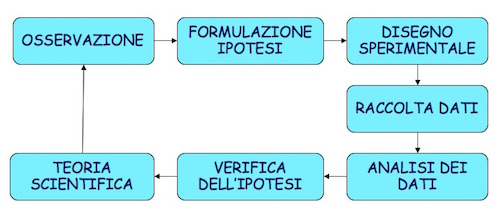
\includegraphics[width=0.75\linewidth]{_images/MSAMap} 

}

\caption{Il metodo scientifico Galileiano}\label{fig:figName11}
\end{figure}

Senza andare troppo in profondità, è importante notare due aspetti:

\begin{enumerate}
\def\labelenumi{\arabic{enumi}.}
\tightlist
\item
  il ruolo fondamentale dell'esperimento scientifico, che produce dati a supporto di ipotesi pre-esistenti;
\item
  lo sviluppo di teorie basate sui dati, che rimangono valide fino a che non si raccolgono altri dati che le confutano, facendo nascere nuove ipotesi che possono portare allo sviluppo di nuove teorie, più affidabili o più semplici.
\end{enumerate}

Insomma, l'ingrediente fondamentale di una prova scientifica è quello di essere supportata dai dati sperimentali: di fatto, non esiste scienza senza dati! Resta famoso l'aforisma ``In God we trust, all the others bring data'', attribuito all'ingegnere e statistico americano W. Edwards Deming (1900-1993), anche se pare che egli, in realtà, non l'abbia mai pronunciato.

\hypertarget{dati-buoni-e-cattivi}{%
\section{Dati `buoni' e `cattivi'}\label{dati-buoni-e-cattivi}}

Detto che la scienza si basa sui dati, bisogna anche dire che non tutti i dati sono ugualmente `buoni'. Nelle scienze biologiche, così come nelle altre scienze, è importante che i dati siano in grado di cogliere gli effetti che vogliamo studiare, senza introdurre distorsioni.

In agricoltura e nelle altre scienze quantitative abbiamo a che fare con fenomeni `misurabili' e, di conseguenza, i nostri dati consistono di un set di misure di diverso tipo (ci torneremo nel secondo capitolo). L'aspetto più importante è che, per tutta una serie di motivi che dettaglieremo tra poco, le nostre misure non necessariamente riflettono il valore vero della caratteristica misurata nel nostro soggetto. Ciò è noto con il termine di \textbf{errore sperimentale}, che non significa che abbiamo necessariamente fatto qualcosa di sbagliato. Anzi, l'errore sperimentale è considerato una componente inevitabile di ogni esperimento, in grado di proiettare un alea d'incertezza su ogni risultato scientifico.

Ci sono tre fondamentali fonti di errore sperimentale:

\begin{enumerate}
\def\labelenumi{\arabic{enumi}.}
\tightlist
\item
  Errore di misura
\item
  Variabilità dei soggetti sperimentali
\item
  Campionamento
\end{enumerate}

Gli errori di misura sono legati allo strumento e dipendono dall'errata taratura, dall'impiego di un protocollo sbagliato, da inesattezze strumentali, da errori nella trascrizione dei risultati oppure dall'irregolarità dell'oggetto da misurare. Ad esempio, pensate alla misurazione dell'altezza di una pianta di mais: è facile riscontrare difficoltà legate, ad esempio, all'individuazione del punto esatto in cui inizia il culmo e del punto esatto dove termina l'infiorescenza apicale.

A parte gli errori di misura, ci sono anche altre sorgenti di errore meno evidenti e legate al fatto che, nel lavoro sperimentale, siamo di solito interessati non ad un singolo soggetto, ma ad un gruppo più o meno numeroso. Ad esempio, se dobbiamo misurare l'effetto di un erbicida, non possiamo farlo trattando una sola pianta, ma dobbiamo ripetere le misure su un gruppo di piante, il che ci porta ad avere un gruppo di misure, una diversa dall'altra. Quindi, qual è l'effetto dell'erbicida? Il fatto di avere tanti effetti diversi quante sono le piante studiate crea comunque un certo grado di variabilità che non dipende da alcun errore tecnico, ma è una caratteristica intrinseca del fenomeno biologico in studio.

Di per se', la variabilità naturale dei soggetti sperimentali non sarebbe un grosso problema, in quanto potremmo calcolarci l'effetto medio e ritenerci soddisfatti in relazione alle finalità dell'esperimento. Tuttavia sorge un nuovo problema legato al fatto che spesso i soggetti sono così numerosi che non possiamo misurarli tutti e siamo costretti a misurare un campione composto da un ridotto numero di individui. Abbiamo un nuovo elemento di incertezza: come facciamo ad essere sicuri che la media, o qualunque altra statistica, misurata nel nostro campione rifletta la media dell'intera popolazione? Anche se abbiamo fatto del tutto per scegliere un campione rappresentativo, è evidente che il campione perfetto non esiste: cosa potrebbe succedere se prendessimo un altro campione?

\hypertarget{dati-buoni-e-metodi-buoni}{%
\section{Dati `buoni' e metodi `buoni'}\label{dati-buoni-e-metodi-buoni}}

Quindi la ricerca scientifica non è esente da `errori' in senso lato (componenti di incertezza). Tuttavia, gli errori non sono tutti uguali e si dividono in \textbf{sistematici} ed \textbf{accidentali (casuali)}. L'errore sistematico è provocato da difetti intrinseci dello strumento o incapacità peculiari dell'operatore e tende a ripetersi costantemente e con lo stesso segno in misure successive. Un esempio tipico è quello di una bilancia non tarata, che tende ad aggiungere 20 grammi ad ogni misura che effettuiamo. D'altra parte, l'errore accidentale, essendo di natura casuale, tende a ripresentarsi con valori e segni diversi. Di conseguenza, è ragionevole pensare che le repliche, nel lungo periodo, producano sovrastime e sottostime con uguale probabilità, in modo che la media tende a coincidere con il valore vero.

È facile capire che le conseguenze degli errori sistematici e accidentali sono ben diverse. A questi proposito, dobbiamo considerare due aspetti molto importanti, cioè:

\begin{enumerate}
\def\labelenumi{\arabic{enumi}.}
\tightlist
\item
  precisione
\item
  accuratezza
\end{enumerate}

Con il termine \textbf{precisione} intendiamo due cose: la prima è relativa al numero di decimali che ci fornisce il nostro strumento di misura. E'evidente, ad esempio, come un calibro sia più preciso di un metro da sarto. Oltre a questo significato, abbastanza intuitivo, ce n'è un altro, più specificatamente legato agli esperimenti scientifici: la precisione di un dato ottenuto attraverso un processo di misurazione non è altro che la variabilità riscontrata quando la misurazione viene ripetuta più volte. L'errore casuale produce sempre un calo di precisione.

Il termine accuratezza ha invece un significato completamente diverso, riconducibile alla differenza tra la misura effettuata e il valore vero della caratteristica da misurare. Può sembrare una banalità, ma proviamo a pensare ad uno strumento non tarato, come, ad esempio, un gascromatografo, che restituisce sempre una concentrazione maggiorata del 20\%. Se noi ripetessimo le analisi 100 volte, in assenza di altri errori, otterremmo sempre lo stesso risultato, molto preciso, ma totalmente inaffidabile, nel senso che non riflette la concentrazione reale della soluzione in studio. L'errore sistematico, oltre a produrre un calo di precisione, produce anche inaccuratezza.

Comprendiamo bene che l'accuratezza è più importante della precisione: infatti una misura accurata, ma imprecisa, riflette bene la realtà, anche se in modo vago. Al contrario, una misura precisa, ma inaccurata, ci porta completamente fuori strada, perché non riflette la realtà. Con linguaggio tecnico, un dato non accurato si dice `distorto' (\emph{biased}) e, siccome la distosione dipende dagli errori sistematici, questi ultimi vanno assolutamente evitati, ad esempio con la perfetta taratura degli strumenti e l'adozione di metodi di misura rigidamente standardizzati e accettati dalla comunità scientifica mondiale.

L'inaccuratezza preoccupa molto i laboratori di analisi, che spesso utilizzano standard di confronto, la cui misura è perfettamente nota e viene periodicamente confrontata con quella rilevabile dallo strumento stesso, per verificarne la taratura. Altro metodo utilizzato nelle procedure di accreditamento dei laboratori è il \emph{ring test}, dove campioni reali della matrice da misurare sono inviati a più laboratori a livello nazionale, in modo da poter confrontare le misure ottenute e valutarne la variabilità. Con un \emph{ring test}, un laboratorio può valutare la sua stessa affidabilità in confronto con laboratori simili, basandosi sull'eventuale differenza tra il risultato ottenuto e quelli ottenuti in tutti gli altri laboratori valutati.

Sfortunatamente la possibilità di raccogliere dati inaccurati è tutt'altro che remota. Gli scienziati americani Pons e Fleischmann, il 23 Marzo del 1989, diffusero pubblicamente la notizia di essere riusciti a riprodurre la fusione nucleare fredda, causando elevatissimo interesse nella comunità scientifica (Fig. \ref{fig:figName2}). Purtroppo le loro misure erano viziate da una serie di problemi e il loro risultato fu smentito da esperimenti successivi.

\begin{figure}

{\centering 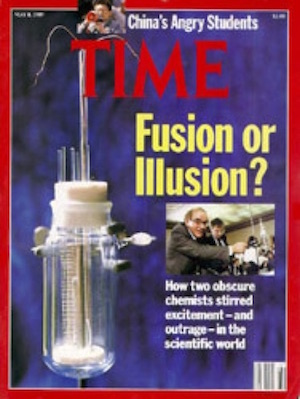
\includegraphics[width=0.5\linewidth]{_images/FalseResults} 

}

\caption{Conseguenze di un esperimento sbagliato}\label{fig:figName2}
\end{figure}

A parte questo clamoroso esempio, torniamo alla nostra domanda iniziale: come facciamo ad essere sicuri che i dati siano validi ed affidabili? La risposta è semplice: non possiamo mai essere sicuri, ma \textbf{dobbiamo fare del nostro meglio per applicare metodi rigorosi, così da minimizzare la possibilità di ottenere errori sistematici}. In altre parole, dati `buoni' sono conseguenza di metodi `buoni' e, pertanto \textbf{una prova scientifica è tale non perché siamo certi che corrisponda alla realtà, ma perché siamo ragionevolmente certi che sia stata ottenuta con metodi validi!}.

\hypertarget{il-principio-di-falsificazione}{%
\section{Il principio di falsificazione}\label{il-principio-di-falsificazione}}

L'approccio che abbiamo indicato poco sopra ha un'importante conseguenza: anche se abbiamo utilizzato un metodo perfettamente valido non potremo mai avere la certezza di aver ottenuto un risultato corrispondente alla realtà e, quindi, ci dovremo sempre aspettare che ulteriori dati smentiscano la nostra conclusione. Questa è la base del principio di falsificazione, definito da Karl Popper (1902-1994): non potremo mai dimostrare che una nostra ipotesi è vera, ma potremo solo dimostrare che è falsa.

In pratica, tornando al metodo scientifico, partiamo da un'ipotesi e organizziamo un esperimento perfettamente valido che produce, di conseguenza, dati validi. Se i nostri dati sconfermano l'ipotesi, abbiamo dimostrato che questa è falsa e dovremo quindi produrre una nuova ipotesi da sottoporre a verifica. Se invece i dati confermano la nostra ipotesi (o meglio, non la smentiscono) allora, non potremo concludere che l'ipotesi è vera, in quanto rimarrà sempre il dubbio che non abbiamo raccolto abbastanza dati. Tuttavia, in mancanza di altre informazioni, prenderemo per buona la nostra ipotesi, fino a che non sarà smentita. Una sorta di `assoluzione' per insufficienza di prove, quindi\ldots{}

Il principio di falsificazione è piuttosto importante nel mondo scientifico ed ha alcune importanti implicazioni:

\begin{enumerate}
\def\labelenumi{\arabic{enumi}.}
\tightlist
\item
  Scienza non necessariamente significa `certezza' o `verità'. Tutto quello che possiamo fare con certezza è rigettare ipotesi (provare che sono false), ma non dimostrarne la validità.
\item
  Il nostro compito è quello di cercare di eliminare tutte le fonti di errore sistematico, per rendere il risultato il più accurato possibile.
\item
  Eliminato l'errore sistematico, l'evantuale errore casuale residuo deve essere sempre quantificato e visualizzato insieme ai risultati.
\item
  In considerazione dell'errore residuo, dobbiamo decidere se i dati raccolti consentono di rigettare la nostra ipotesi di partenza. Altrimenti, l'esperimento è inconclusivo e, pur non avendone la certezza, terremo per vera la nostra ipotesi di partenza fino a che non sarà smentita da future osservazioni.
\end{enumerate}

Oltre al principio di falsificazione, la scienza fa largo uso del principio del `rasoio di Occam'. Guglielmo di Occam (XIV secolo) era un frate francescano che, in un periodo in cui le dimostrazioni scientifiche iniziavano a divenire troppo complesse, voleva ribadire l'importanza della semplicità. Il suo principio è solitamente formulato come `\emph{Entia non sunt multiplicanda praeter necessitatem}' ed è noto come il `rasoio' in quanto porta a respingere con nettezza (tagliare con il rasoio) le spiegazioni troppo complesse. Nella comunità scientifica, applichiamo questo principio preferendo sempre, tra due ipotesi alternative ugualmente buone, quella più semplice.

\hypertarget{falsificare-un-risultato}{%
\section{Falsificare un risultato}\label{falsificare-un-risultato}}

Se un esperimento è inconclusivo e porta ad eccettare un'ipotesi, è sempre possibile eseguire un ulteriore esperimento per rigettarla. Se anche questo secondo esperimento non riesce a rigettare l'ipotesi di partenza, allora la bontà di quest'ultima è certamente rafforzata. Parliamo quindi di esperimenti confermativi che costituiscono un elemento molto importante del metodo scientifico.

A questo proposito, distinguiamo:

\begin{enumerate}
\def\labelenumi{\arabic{enumi}.}
\tightlist
\item
  replicabilità
\item
  riproducibilità
\end{enumerate}

Un esperimento è replicabile se, quando ripetuto in condizioni assolutamente analoghe (stessi soggetti, ambiente, strumenti\ldots), restituisce risultati equivalenti. Per questo motivo, quando si pubblicano i risultati di un esperimento, è sempre necessario descrivere accuratamente i metodi impiegati, in modo da consentire a chiunque la verifica dei risultati.

In alcuni casi, tuttavia, questa verifica indipendente è pressoché impossibile; ad esempio, nelle scienze agronomiche, le caratteristiche genetiche e pedo-climatiche giocano un ruolo molto importante e non è facile replicare un esperimento di pieno campo esattamente nelle stesse condizioni. Per questo motivo, alcuni biostatistici distinguono la replicabilità dalla riproducibilità, definita come il grado di concordanza tra esperimenti ripetuti in condizioni diverse (diversi soggetti, diverso ambiente\ldots). Se la replicabilità di un esperimento non può essere dimostrata, bisogna avere almeno un'idea della sua riproducibilità, ripetendo l'esperimento in condizioni diverse e discutendo attentamente le eventuali differenze riscontrate nei risultati.

\begin{center}\rule{0.5\linewidth}{0.5pt}\end{center}

\hypertarget{elementi-fondamentali-del-disegno-sperimentale}{%
\section{Elementi fondamentali del disegno sperimentale}\label{elementi-fondamentali-del-disegno-sperimentale}}

La metodica di organizzazione di un esperimento valido prende il nome di \emph{disegno sperimentale} e le sue basi si fanno in genere risalire a Sir Ronald A. Fisher, vissuto in Inghilterra dal 7 Febbraio 1890 al 29 luglio 1962. Laureatosi nel 1912, lavora come statistico per il comune di Londra, fino a quando diviene socio della prestigiosa Eugenics Education Society di Cambridge, fondata nel 1909 da Francis Galton, cugino di Charles Darwin. Dopo la fine della guerra, Karl Pearson gli propone un lavoro presso il rinomato Galton Laboratory, ma egli non accetta a causa della profonda rivalità esistente tra lui e Pearson stesso. Nel 1919 viene assunto presso la Rothamsted Experimental Station, dove si occupa dell'elaborazione dei dati sperimentali e, nel corso dei successivi 7 anni, definisce le basi del disegno sperimentale ed elabora la sua teoria della ``analysis of variance''. Il suo libro più importante è ``The design of experiment'', del 1935. E' sua la definizione delle tre componenti fondamentali del disegno sperimentale:

\begin{enumerate}
\def\labelenumi{\arabic{enumi}.}
\tightlist
\item
  controllo degli errori;
\item
  replicazione;
\item
  randomizzazione.
\end{enumerate}

\hypertarget{controllo-degli-errori}{%
\subsection{Controllo degli errori}\label{controllo-degli-errori}}

Controllare gli errori, o, analogamente, eseguire un esperimento controllato significa fondamentalmente due cose:

\begin{enumerate}
\def\labelenumi{\arabic{enumi}.}
\tightlist
\item
  adottare provvedimenti idonei ad evitare le fonti di errore, mantenendole al livello più basso possibile (alta precisione);
\item
  agire in modo da isolare l'effetto in studio (accuratezza), evitando che si confonda con effetti casuali e di altra natura. Ad esempio, se dobbiamo confrontare due fitofarmaci, dobbiamo fare in modo che i soggetti inclusi nell'esperimento differiscano tra di loro solo per il fitofarmaco impiegato e non per altro.
\end{enumerate}

Mettere in pratica questi principi fondamentali richiede una vita di esperienza! Tuttavia, vogliamo solo sottolineare alcuni aspetti, come il rigore metodologico. È evidente che, ad esempio, se vogliamo sapere la cinetica di degradazione di un erbicida a 20 °C dovremo realizzare una prova esattamente a quella temperatura, con un erbicida uniformemente distribuito nel terreno, dentro una camera climatica capace di un controllo perfetto della temperatura. Gli strumenti dovranno essere ben tarati e sarà necessario attenersi scrupolosamente a metodi validati e largamente condivisi. Tuttavia, a proposito di rigore, non bisogna scordare il famoso aforisma, attribuito a C.F. Gauss e riferito alla della precisione nei calcoli, che può essere anche riferito al rigore nella ricerca : ``\emph{Manca di mentalità matematica tanto chi non sa riconoscere rapidamente ciò che è evidente, quanto chi si attarda nei calcoli con una precisione superiore alla necessità}''. In altre parole, il rigore metodologico è fondamentale, ma deve essere sempre compatibile con gli scopi della ricerca ed i livelli di precisione richiesti, per evitare un'eccessivo consumo di tempo e risorse finanziare.

Oltre al rigore metodologico, è bene anche ricordare come un esperimento ben fatto passi sempre attraverso la giusta selezione dei soggetti sperimentali, che debbono essere omogenei, ma rappresentativi della popolazione alla quale intendiamo riferire i risultati ottenuti. Ad esempio, se si vuole ottenere un risultato riferito alla collina umbra, bisognerà scegliere parcelle di terreno omogenee, ma che rappresentano bene la variabilità pedo-climatica di quell'ambiente, né di più, né di meno.

Per concludere, vogliamo anche ricordare le cosiddette `intrusioni' cioè quegli eventi che accadono in modo inaspettato e condizionano negativamente la riuscita di un esperimento in corso. E' evidente che, ad esempio, un'alluvione, l'attacco di insetti o patogeni, la carenza idrica hanno una pesante ricaduta sulla precisione di un esperimento e sulla sua riuscita. Per quanto possibile, controllare gli errori significa anche essere capaci di prevedere le eventuali intrusioni. In un suo famoso lavoro scientifico del 1984, lo scienziato americano Stuart Hurlbert usa il termine `intrusione demoniaca' per indicare quelle intrusioni che, pur casuali, avrebbero potuto essere previste con un disegno più accurato, sottolineando in questo caso la responsabilità dello sperimentatore.

Un esempio è questo: uno sperimentatore vuole studiare l'entità della predazione dovuta alle volpi e quindi usa campi senza staccionate (dove le volpi possono entrare) e campi protetti da staccionate (e quindi liberi da volpi). Se le staccionate, essendo utilizzate dai falchi come punto d'appoggio, finiscono per incrementare l'attività predatoria di questi ultimi, si viene a creare un'intrusione demoniaca, che rende l'esperimento distorto. Il demonio, in questo caso, non è il falco, che danneggia l'esperimento, ma il ricercatore stesso, che non ha saputo prevedere una possibile intrusione.

\hypertarget{replicazione}{%
\subsection{Replicazione}\label{replicazione}}

In ogni esperimento, i trattamenti dovrebbe essere replicati su due o più unità sperimentali. Ciò permette di:

\begin{enumerate}
\def\labelenumi{\arabic{enumi}.}
\tightlist
\item
  dimostrare che i risultati sono replicabili (ma non è detto che siano riproducibili!);
\item
  rassicurare che eventuali circostanze aberranti casuali non abbiano provocato risultati distorti;
\item
  misurare la precisione dell'esperimento, come variabilità di risposta tra repliche trattate nello stesso modo;
\item
  incrementare la precisione dell'esperimento (più sono le repliche più l'esperimento è preciso, perché si migliora la stima della caratteristica misurata, diminuendo l'incertezza).
\end{enumerate}

Per poter essere utili, le repliche debbono essere indipendenti, cioè debbono \textbf{aver subito tutte le manipolazioni necessarie per l'allocazione del trattamento in modo totalmente indipendente l'una dall'altra}. Le manipolazioni comprendono tutte le pratiche necessarie, come ad esempio la preparazione delle soluzioni, la diluizione dei prodotti, ecc..

La manipolazione indipendente è fondamentale, perché in ogni parte del processo di trattamento possono nascondersi errori più o meno grandi, che possono essere riconosciuti solo se colpiscono in modo casuale le unità sperimentali. Se la manipolazione è, anche solo in parte, comune, questi errori colpiscono tutte le repliche allo stesso modo, diventano sistematici e quindi non più riconoscibili. Di conseguenza, si inficia l'accuratezza dell'esperimento. Quando le repliche non sono indipendenti, si parla di \textbf{pseudorepliche}, contrapposte alle \textbf{repliche vere}.

Il numero di repliche dipende dal tipo di esperimento: più sono e meglio è, anche se è necessario trovare un equilibrio accettabile tra precisione e costo dell'esperimento. Nella sperimentazione di campo, due repliche sono poche, tre appena sufficienti, quattro costituiscono la situazione più comune, mentre un numero maggiore di repliche è abbastanza raro, non solo per la difficoltà di seguire l'esperimento, ma anche perché aumentano la dimensione della prova e, di conseguenza, la variabilità del terreno.

\hypertarget{randomizzazione}{%
\subsection{Randomizzazione}\label{randomizzazione}}

L'indipendenza di manipolazione non garantisce da sola un esperimento corretto. Infatti potrebbe accadere che le caratteristiche innate dei soggetti, o una qualche `intrusione' influenzino in modo sistematico tutte le unità sperimentali trattate nello stesso modo, così da confondersi con l'effetto del trattamento. Un esempio banale è che potremmo somministrare un farmaco a quattro soggetti in modo totalmente indipendente, ma se i quattro soggetti fossero sistematicamente più alti di quelli non trattati finiremmo per confondere una caratteristica innata con l'effetto del farmaco. Oppure, se le piante di una certa varietà di sorgo si trovassero tutte più vicine alla scolina rispetto a quelle di un'altra varietà, potrebbero essere più danneggiate dal ristagno idrico, il cui effetto si confonderebbe con quello del trattamento stesso.

Questi problemi sono particolarmente insidiosi e si nascondono anche dietro ai particolari apparentemente più insignificanti. La randomizzazione è l'unico sistema per evitare, o almeno rendere molto improbabile, la confusione dell'effetto del trattamento con fattori casuali e/o comunque diversi dal trattamento stesso. La randomizzazione si declina in vari modi:

\begin{enumerate}
\def\labelenumi{\arabic{enumi}.}
\tightlist
\item
  allocazione casuale del trattamento alle unità sperimentali. Gli esperimenti che prevedono l'allocazione del trattamento sono detti `manipolativi' o `disegnati'.
\item
  A volte l'allocazione del trattamento non è possibile o non è etica. Se volessimo studiare l'effetto delle cinture di sicurezza nell'evitare infortuni gravi, non potremmo certamente provocare incidenti deliberati. In questo caso la randomizzazione è legata alla scelta casuale di soggetti che sono `naturalmente' trattati. Esperimenti di questi tipo, si dicono \textbf{osservazionali}. Un esempio è la valutazione dell'effetto dell'inquinamento con metalli pesanti nella salute degli animali: ovviamente non è possibile, se non su piccola scala, realizzare il livello di inquinamento desiderato e, pertanto, dovremo scegliere soggetti che sono naturalmente sottoposti a questo genere di inquinamento, magari perché vivono vicino a zone industriali.
\item
  Se i soggetti sono immobili, la randomizzazione ha anche una connotazione legata alla disposizione spaziale e/o temporale casuale.
\end{enumerate}

L'assegnazione casuale del trattamento, o la selezione casuale dei soggetti trattati, fanno si che tutti i soggetti abbiano la stessa probabilità di ricevere qualunque trattamento oppure qualunque intrusione casuale. In questo modo, la probabilità che tutte le repliche di un trattamento abbiano qualche caratteristica innata o qualche intrusione comune che li penalizzi/avvantaggi viene minimizzata. Di conseguenza, confondere l'effetto del trattamento con variabilità casuale (`confounding'), anche se teoricamente possibile, diviene altamente improbabile.

\hypertarget{esperimenti-invalidi}{%
\subsection{Esperimenti invalidi}\label{esperimenti-invalidi}}

A questo punto, dovrebbe essere chiaro che un esperimento valido deve essere controllato, replicato e randomizzato: la mancanza anche di uno solo di questi elementi pone dubbi ragionevoli sull'affidabilità dei risultati. In particolare, gli esperimenti `invalidi' sono caratterizzati da:

\begin{enumerate}
\def\labelenumi{\arabic{enumi}.}
\tightlist
\item
  Cattivo controllo degli errori
\item
  Fondati sospetti di confounding
\item
  Mancanza di repliche vere
\item
  Confusione tra repliche vere e pseudo-repliche
\item
  Mancanza di randomizzazione
\item
  Presenza di vincoli alla randomizzazione, trascurati in fase di analisi.
\end{enumerate}

Le conseguenze di queste problematiche sono abbastanza diverse.

\hypertarget{cattivo-controllo-degli-errori}{%
\subsubsection{Cattivo controllo degli errori}\label{cattivo-controllo-degli-errori}}

Bisogna verificare se il problema è relativo a questioni come la mancanza di scrupolosità, l'uso di soggetti poco omogenei o di un ambiente poco omogeneo, o altri aspetti che inficiano solo la precisione, ma non l'accuratezza dell'esperimento. In questo caso, l'esperimento è ancora valido (accurato), ma la bassa precisione probabilmente impedirà di trarre conclusioni forti. Quindi, un esperimento impreciso si `elimina' da solo, perché sarà inconclusivo. Di questi esperimenti bisogna comunque diffidare, soprattutto quando siano pianificati per mostrare l'assenza di differenze tra due trattamenti alternativi. Mostrare l'assenza di differenze è facile: basta fare male un esperimento, in modo che vi sia un alto livello di incertezza e quindi l'evidenza scientifica sia molto debole.

Diversa è la situazione in cui un cattivo controllo degli errori, ad esempio l'adozione di metodi sbagliati, porta a mancanza di accuratezza, cioè a risultati che non riflettono la realtà (campionamento sbagliato, ad esempio; oppure strumenti non tarati; impiego di metodi non validati e/o non accettabili). In questo caso venendo a mancare l'accuratezza, l'esperimento deve essere rigettato, in quanto non fornisce informazioni realistiche.

\hypertarget{confounding-e-correlazione-spuria}{%
\subsubsection{`Confounding' e correlazione spuria}\label{confounding-e-correlazione-spuria}}

Abbiamo appena menzionato il problema fondamentale della ricerca, cioè il \textbf{confounding}, vale a dire la confusione tra l'effetto del trattamento e un qualche altro effetto casuale, legato alle caratteristiche innate del soggetto o a qualche intrusione più o meno `demoniaca'. Abbiamo detto che non possiamo mai avere la certezza dell'assenza di confounding, ma abbiamo anche detto che l'adozione di una pratica sperimentale corretta ne minimizza la probabilità.

Chiaramente, rimangono dei rischi che sono tipici di situazioni nelle quali il controllo adottato non è perfetto, come capita, ad esempio, negli esperimenti osservazionali. In questo ambito è piuttosto temuta la cosiddetta `correlazione spuria', una forma di confounding casuale per cui due variabili variano congiuntamente (sono direttamente o inversamente proporzionali), ma in modo del tutto casuale. Esistono, ad esempio, dati che mostrano una chiara correlazione tra le vendite di panna acida e le morti per incidenti in motocicletta (Fig. \ref{fig:figName22}). Chiaramente, non esistono spiegazioni scientifiche per questo effetto, che è, ovviamente, del tutto casuale. Il problema è che questa correlazione spuria non è sempre così semplice da rintracciare.

\begin{figure}

{\centering 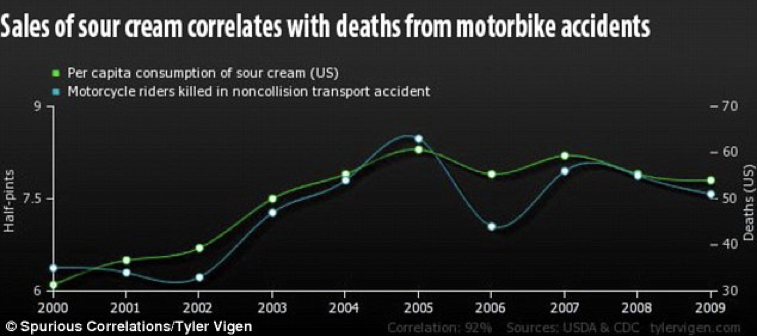
\includegraphics[width=0.9\linewidth]{_images/PannaAcida} 

}

\caption{Esempio di correlazione spuria}\label{fig:figName22}
\end{figure}

A volte il confounding non è casuale, ma è legato ad una variabile esterna che si agisce all'insaputa dello sperimentatore. Ad esempio, è stato osservato che il tasso di crimini è più alto nelle città che hanno più chiese. La spiegazione di questo paradosso sta nel fatto che esiste un `confounder', cioè l'ampiezza della popolazione. Nelle grandi città si riscontrano sia una maggiore incidenza criminale, sia un grande numero di chiese. In sostanza, la popolazione determina sia l'elevato numero di chiese che l'elevato numero di crimini, ma queste ultime due variabili non sono legate tra loro da una relazione causa-effetto (A implica B e A implica C, ma B non implica C).

Il confounding non casuale è spesso difficile da evidenziare, soprattutto se le correlazioni misurate sono spiegabili. Inoltre, non è eliminabile con un'accurata randomizzazione, ma solo con l'esecuzione di un esperimento totalmente controllato, nel quale ci si preoccupa di rilevare tutte le variabili necessarie per spiegare gli effetti riscontrati. Di questo è importante tener conto soprattutto negli esperimenti osservazionali, dove il controllo è sempre più difficile e meno completo.

\hypertarget{pseudo-repliche-e-randomizzazione-poco-attenta}{%
\subsubsection{Pseudo-repliche e randomizzazione poco attenta}\label{pseudo-repliche-e-randomizzazione-poco-attenta}}

Per evidenziare questi problemi e comprendere meglio la differenza tra un esperimento corretto e uno non corretto, è utilissima la classificazione fatta da Hurlbert (1984), che riportiamo in Figura \ref{fig:figName23}.

\begin{figure}

{\centering 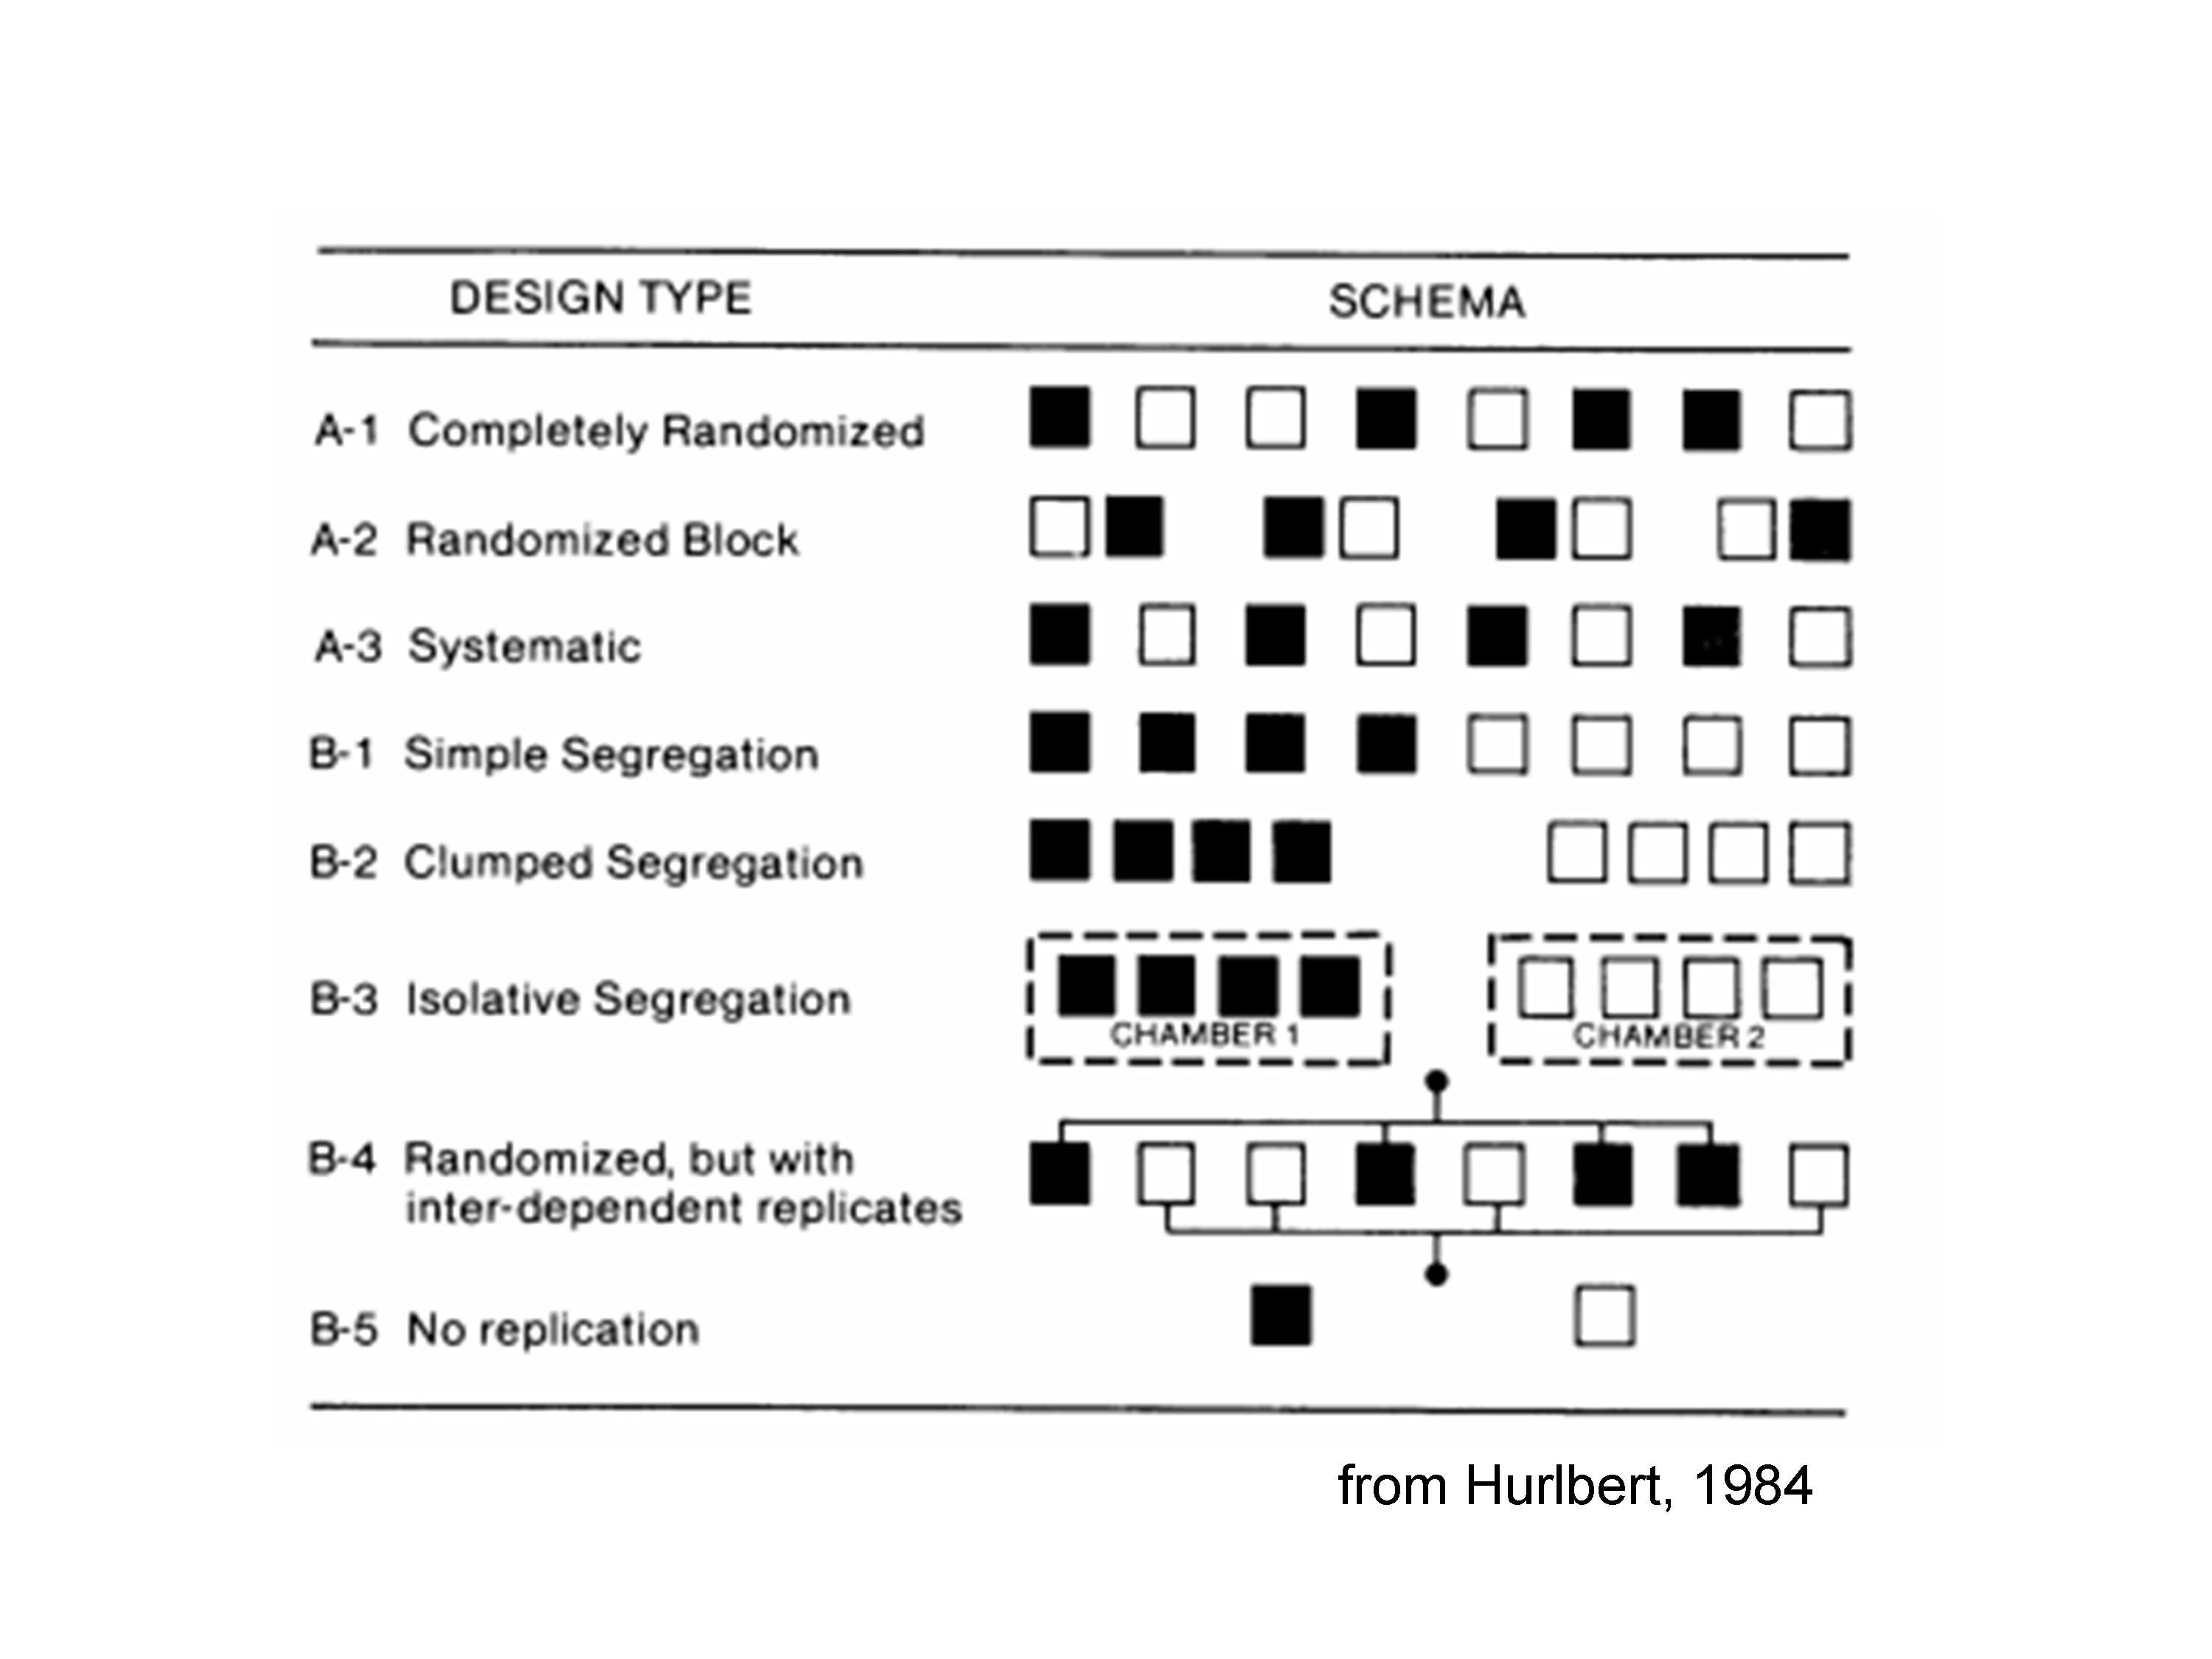
\includegraphics[width=0.9\linewidth]{_images/Randomisation} 

}

\caption{Indicazioni per una corretta randomizzazione (Hurlbert, 1984)}\label{fig:figName23}
\end{figure}

Vengono mostrati 8 soggetti, sottoposti a due trattamenti (bianco e nero), con 8 disegni sperimentali diversi.

Il disegno A1 è corretto, in quanto si tratta di un esperimento completamente randomizzato. Ugualmente, è valido il disegno A2, nel quale le unità sperimentali sono state divise in quattro gruppi omogenei e sono state trattate in modo randomizzato all'interno di ogni gruppo.

Il disegno A3 è quantomeno `sospetto': vi sono repliche vere, ma l'allocazione dei trattamenti non è randomizzata ed avviene con un processo sistematico per il quale `nero' e `bianco' si alternano. Cosa succederebbe se vi fosse un gradiente di fertilità decrescente da destra verso sinistra? Le unità nere sarebbero avvantaggiate rispetto alle bianche! Insomma, rimangono sospetti di confounding, a meno che non si sia assolutamente certi dell'assenza di gradienti, come capita ad esempio se all'interno dei blocchi, dobbiamo creare una sequenza spazio-temporale. Vediamo tre esempi:

\begin{enumerate}
\def\labelenumi{\arabic{enumi}.}
\tightlist
\item
  ho quattro piante e, per ogni pianta, voglio confrontare un ramo basso con uno alto: è evidente che i due trattamenti sono sempre ordinati in modo sistematico (basso prima di alto).
\item
  Dobbiamo valutare l'effetto di fitofarmaci somministrati in due epoche diverse (accestimento e inizio-levata); anche qui non possiamo randomizzare, giacché un'epoca precede sempre l'altra.
\item
  Dobbiamo confrontare la presenza di residui di un fitofarmaco a due profondità e non possiamo randomizzare, perché una profondità precede sempre l'altra nello spazio.
\end{enumerate}

In queste situazioni l'esperimento rimane valido, anche se la randomizzazione segue un processo sistematico e non casuale.

Il disegno B1 è usualmente invalido: non vi è randomizzazione e ciò massimizza i problemi del disegno A3: la separazione delle unità sperimentali `bianche' e `nere' non consente una valutazione adeguata dell'effetto del trattamento, che è confuso con ogni potenziale differenza tra la parte destra e la sinistra dell'ambiente in cui la sperimentazione viene eseguita. Ovviamente, la separazione può essere non solo spaziale, ma anche temporale. Anche in questo caso diamo alcuni esempi in cui una situazione come quella descritta in B1 è valida:

\begin{enumerate}
\def\labelenumi{\arabic{enumi}.}
\tightlist
\item
  Vogliamo confrontare la produzione in pianura e in collina. Ovviamente dobbiamo scegliere campioni in due situazioni fisicamente separate
\item
  Vogliamo confrontare la pescosità di due laghetti
\item
  Vogliamo confrontare la produttività di due campi contigui.
\end{enumerate}

Queste situazioni sono valide, anche se con una restrizione: non siamo in grado di stabilire a chi debba essere attribuito l'effetto. Ad esempio, per la prima situazione, pianura e collina possono dare produzioni diverse per il suolo diverso, il clima diverso, la precessione colturale diversa o un qualunque altro elemento che differenzi le due località.

Il disegno B2 è analogo al disegno B1, ma il problema è più grave, perché la separazione fisica è più evidente. Questo disegno è totalmente sbagliato, a meno che non siamo specificatamente interessati all'effetto località (vedi sopra).

Il disegno B3 è analogo al disegno B2, ma costituisce una situazione molto frequente nella pratica scientifica. Immaginiamo infatti di voler confrontare la germinazione dei semi a due temperature diverse, utilizzando due camere climatiche e mettendo, in ognuna di esse, quattro capsule Petri identiche. In questa situazione, l'effetto temperatura è totalmente confuso con l'effetto `camera climatica (località)' e risente di ogni malfunzionamento relativo ad una sola delle due camere. Inoltre, le unità sperimentali con lo stesso trattamento di temperature non sono manipolate in modo indipendente, dato che condividono la stessa camera climatica. Di conseguenza, non si può parlare di repliche vere, bensì di \textbf{pseudorepliche}.

Altri esempi di \textbf{pseudorepliche} sono schematizzati con il codice B4. Ad esempio:

\begin{enumerate}
\def\labelenumi{\arabic{enumi}.}
\tightlist
\item
  trattare piante in vaso ed analizzare in modo indipendente i singoli individui invece che tutto il vaso;
\item
  trattare una parcella di terreno e prelevare da essa più campioni, analizzandoli separatamente;
\item
  trattare una capsula Petri ed analizzare separatamente i semi germinati al suo interno.
\end{enumerate}

Questi disegni, in assenza di repliche vere aggiuntive non sono da considerarsi validi. Ad esempio, se io ho due vasetti trattati in modo totalmente indipendente e da ciascuno di essi prelevo due piante e le analizzo separatamente, il disegno è caratterizzato da due repliche vere e due pseudorepliche per ogni replica ed è, pertanto, valido.

Il disegno B5 è invece evidentemente invalido, per totale mancanza di repliche.

\hypertarget{chi-valuta-se-un-esperimento-uxe8-attendibile}{%
\section{Chi valuta se un esperimento è attendibile?}\label{chi-valuta-se-un-esperimento-uxe8-attendibile}}

Quanto detto finora vorrebbe chiarire come il punto centrale della scienza non è la certezza delle teorie, bensì il metodo che viene utilizzato per definirle. Ognuno di noi è quindi responsabile di verificare che le informazioni in suo possesso siano `scientificamente' attendibili, cioè ottenute con un metodo sperimentale adeguato. Il fatto è che non sempre siamo in grado di compiere questa verifica, perché non abbiamo strumenti `culturali' adeguati, se non nel ristretto ambito delle nostre competenze professionali. Come fare allora?

L'unica risposta accettabile è quella di controllare l'attendibilità delle fonti di informazione. In ambito biologico, le riviste autorevoli sono caratterizzate dal procedimento di `\emph{peer review}', nel quale i manoscritti scientifici, prima della pubblicazione, sono sottoposti ad un comitato editoriale ed assegnati ad un `editor', il quale legge il lavoro e contemporaneamente lo invia a due o tre scienziati anonimi e particolarmente competenti in quello specifico settore scientifico (\emph{reviewers} o revisori).

I revisori, insieme all'\emph{editor}, compiono un attento lavoro di esame e stabiliscono se l'evidenza scientifica presentata è sufficientemente `forte'. Le eventuali critiche vengono presentate all'autore, che è tenuto a rispondere in modo convincente, anche ripetendo gli esperimenti se necessario. Il processo richiede spesso interi mesi ed è abbastanza impegnativo per uno scenziato. E' piuttosto significativa l'immagine presentata in \href{http://scienceblogs.com/startswithabang/2013/06/07/the-4-jobs-of-a-referee-in-peer-review/}{scienceBlog.com}, che allego qui.

\begin{figure}

{\centering 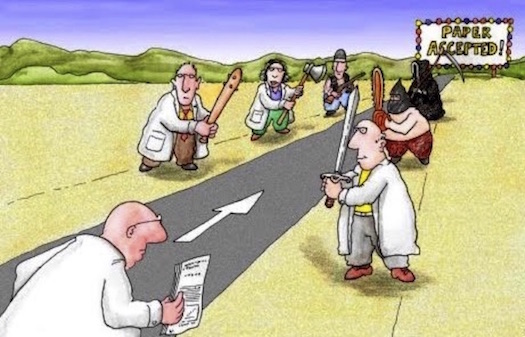
\includegraphics[width=0.75\linewidth]{_images/PeerReview} 

}

\caption{Il processo di peer review}\label{fig:figName3}
\end{figure}

In sostanza il meccanismo di \emph{peer review} porta a rigettare un lavoro scientifico in presenza di qualunque ragionevole dubbio metodologico. Desideriamo sottolineare che abbiamo parlato di dubbio metodologico, dato che il dubbio sul risultato non può essere allontanato completamente e i reviewer controlleranno solo che il rischio di errore sia al disotto della soglia massima arbitrariamente stabilita (di solito pari al 5\%). Questo procedimento, se effettuato con competenza, dovrebbe aiutare a separare la scienza dalla pseudo-scienza e, comunque, ad eliminare la gran parte degli errori metodologici dai lavori scientifici.

\hypertarget{conclusioni}{%
\section{Conclusioni}\label{conclusioni}}

In conclusione, possiamo ripartire dalla domanda iniziale: ``Che cosa è la scienza?'', per rispondere che è scienza tutto ciò che è supportato da dati che abbiano passato il vaglio della \emph{peer review}, dimostrando di essere stati ottenuti con un procedimento sperimentale privo di vizi metodologici e di essere sufficientemente affidabili in confronto alle fonti di incertezza cui sono associati.

Qual è il \emph{take-home message} di questo capitolo? Fidatevi solo delle riviste scientifiche attendibili, cioè quelle che adottano un serio processo di \emph{peer review} prima della pubblicazione.

\hypertarget{esercizi-e-domande}{%
\section{Esercizi e domande}\label{esercizi-e-domande}}

\begin{center}\rule{0.5\linewidth}{0.5pt}\end{center}

\hypertarget{altre-letture}{%
\section{Altre letture}\label{altre-letture}}

\begin{enumerate}
\def\labelenumi{\arabic{enumi}.}
\tightlist
\item
  Fisher, Ronald A. (1971) {[}1935{]}. The Design of Experiments (9th ed.). Macmillan. ISBN 0-02-844690-9.
\item
  Hurlbert, S., 1984. Pseudoreplication and the design of ecological experiments. Ecological Monographs, 54, 187-211
\item
  Kuehl, R. O., 2000. Design of experiments: statistical principles of research design and analysis. Duxbury Press (CHAPTER 1)
\end{enumerate}

\hypertarget{progettare-un-esperimento}{%
\chapter{Progettare un esperimento}\label{progettare-un-esperimento}}

\hypertarget{gli-elementi-della-ricerca}{%
\section{Gli elementi della ricerca}\label{gli-elementi-della-ricerca}}

Nel capitolo precedente abbiamo visto che ogni esperimento, per essere valido, deve conformarsi a tre principi di base, cioè la replicazione, la randomizzazione e il controllo. Non è facile spiegare come si mettano in atto questi principi e, certamente, non esiste una risposta generalmente valida; l'esperienza gioca un ruolo fondamentalmente e, quando si muovono i primi passi, è sempre bene cercare l'aiuto di un collega più anziano.

In questo capitolo prenderemo in esame una serie di elementi che riguardano tutti gli esperimenti scientifici, indipendentemente dalla disciplina e dalle finalità. Per la loro importanza, ognuno di questi elementi richiederà decisioni opportune in fase di pianificazione e dovrà essere accuratamente dettagliato in ogni progetto o rapporto di ricerca, per permettere la valutazione della bontà della ricerca stessa. Questi elementi sono:

\begin{enumerate}
\def\labelenumi{\arabic{enumi}.}
\tightlist
\item
  ipotesi ed obiettivi
\item
  fattore/i sperimentale/i;
\item
  soggetti sperimentali (unità sperimentali);
\item
  allocazione dei trattamenti;
\item
  le variabili sperimentali.
\end{enumerate}

\hypertarget{ipotesi-scientifica-rightarrow-obiettivo-dellesperimento}{%
\section{\texorpdfstring{Ipotesi scientifica \(\rightarrow\) obiettivo dell'esperimento}{Ipotesi scientifica \textbackslash rightarrow obiettivo dell'esperimento}}\label{ipotesi-scientifica-rightarrow-obiettivo-dellesperimento}}

Trascurando la ricerca bibliografica, che è pur fondamentale, nel metodo scientifico galileiano, il punto di partenza di un esperimento è l'\textbf{ipotesi scientifica}, dalla quale discende tutto il lavoro successivo. Questa ipotesi deve essere rilevante, chiaramente definita e specifica; insomma, dobbiamo aver individuato con chiarezza una connessione tra eventi che potrebbe essere spiegata da una relazione causa-effetto. Un ipotesi, solitamente si pone in forma dubitativa: ``\emph{la germinazione di un lotto di semi potrebbe dipendere dall'adozione di un certo metodo di priming}''; oppure: ``\emph{la produttività di una coltura potrebbe migliorare con l'adozione di una maggiore fittezza d'impianto}''.

Dall'ipotesi, in modo consequenziale scaturiscono gli obiettivi della ricerca, cioè le domande alle quali la ricerca intende dare risposta. Questi obiettivi dovranno essere raggiungibili/realistici e temporalmente organizzati; inoltre, dovrà essere possibile capire se e quando siano stati raggiunti attraverso un qualche indicatore misurabile.

Il rischio che si corre con obiettivi mal posti è quello di eseguire una ricerca dispersiva, con raccolta di dati non necessari e/o mancanza di dati fondamentali, con costi più elevati del necessario e un uso poco efficiente delle risorse. In genere, prima si definisce un obiettivo generale, poi si definiscono uno o più obiettivi specifici, proiettati su un più breve spazio temporale, anche per marcare le fasi necessarie per raggiungere l'obiettivo generale.

Non è un caso se, in un lavoro scientifico, gli obiettivi della ricerca sono posti in fondo all'introduzione, appena prima dell'esposizione dei materiali e metodi.

\hypertarget{identificazione-dei-fattori-sperimentali}{%
\section{Identificazione dei fattori sperimentali}\label{identificazione-dei-fattori-sperimentali}}

A differenza degli esperimenti \textbf{osservazionali}, più tipici delle scienze mediche e sociali, dove ci si limita ad osservare quanto accade in natura, gli esperimenti \textbf{manipolativi} sono basati appunto sulla `manipolazione' dei soggetti sperimentali, che vengono sottoposti a stimoli differenti, a seconda della risposta che si vuole valutare.

Dopo aver definito l'obiettivo di un esperimento, pertanto, è necessario chiarire esattamente quali saranno gli stimoli ai quali sottoporremo le unità sperimentali. Uno `stimolo' sperimentale prende il nome di \textbf{fattore sperimentale}, che può avere più \textbf{livelli}, detti \textbf{trattamenti (o tesi) sperimentali}. Ad esempio, se l'obiettivo è quello di valutare l'effetto della temperatura sulla germinazione dei semi di quinoa, il fattore sperimentale sarà la temperatura, con tre livelli, 10, 15 e 25°C, ai quali verranno sottoposte le capsule Petri incluse in prova.

\hypertarget{esperimenti-multi-fattoriali}{%
\subsection{Esperimenti (multi-)fattoriali}\label{esperimenti-multi-fattoriali}}

Talvolta gli obiettivi dell'esperimento comportano lo studio di più di un fattore sperimentale; ad esempio, oltre che alla temperatura, potremmo anche essere interessati a studiare l'effetto dell'umidità sulla germinazione dei semi. In questo caso potremmo pianificare due esperimenti separati oppure un unico esperimento, in cui prendiamo in considerazione entrambi i fattori sperimentali. Un esperimenti di questo tipo si dice \textbf{fattoriale}, o meglio, \textbf{multi-fattoriale} ed i fattori possono essere \textbf{incrociati (crossed)} oppure \textbf{innestati}. Nel primo caso includeremo in prova tutte le possibili combinazioni tra i livelli di ogni fattore. Ad esempio, se volessimo studiare il comportamento di tre varietà di girasole (A, B e C) con due tipi di concimi (pollino e urea), potremmo disegnare un esperimento con 6 trattamenti, rappresentati da tutte le possibili combinazioni di varietà e concimi, cioè A-pollina, A-urea, B-pollina, B-urea, C-pollina e C-urea.

In un disegno a fattori innestati, invece, i livelli di un fattore cambiano al cambiare dei livelli dell'altro. Ad esempio, se volessimo confrontare tre varietà di frumento in due sistemi colturali (convenzionale e biologico), potremmo decidere di utilizzare varietà diverse in sistemi diversi, alla ricerca del miglior adattamento possibile per una certa specie. In questo caso avremmo comunque sei trattamenti, ma le combinazioni sarebbero: biologico-A, biologico-B, biologico-C, convenzionale-D, convenzionale-E e convenzionale-F.

Il vantaggio degli esperimenti fattoriali è che permettono di valutare la presenza di `interazione', un fenomeno che si produce quando le combinazioni tra alcuni dei livelli inclusi in prova per ogni fattore producono risposte inattese, particolarmente buone o cattive rispetto a quello che avremmo potuto attenderci, considerando i due fattori sperimentali uno separatamente dall'altro. Ad esempio, se considerassimo le due varietà di mais A e B, con A mediamente più produttiva di B, coltivate in due annate, ad esempio 2025 e 2026, con la seconda molto più sfavorevole, perché siccitosa, dovremmo aspettarci che la combinazione A-2025 fornisca i migliori risultati, mentre la combinazione B-2026 fornisca i peggiori. Se questo non avviene, ad esempio perché B è particolarmente adatta a resistere alla siccità, allora abbiamo un fenomeno d'interazione, che è molto importante studiare nel dettaglio, con un esperimento fattoriale.

\hypertarget{controllo-o-testimone}{%
\subsection{Controllo o testimone}\label{controllo-o-testimone}}

In alcuni casi è necessario inserire in prova un trattamento che funga da riferimento per tutti gli altri; questo trattamento è comunemente detto \textbf{controllo} o \textbf{testimone}. Possiamo avere:

\begin{enumerate}
\def\labelenumi{\arabic{enumi}.}
\tightlist
\item
  controllo non trattato
\item
  controllo trattato con placebo
\item
  controllo trattato secondo le modalità usuali
\end{enumerate}

Il controllo cosiddetto `non trattato' è tipico degli esperimenti in ambito fitopatologico, ad esempio quando si vogliono confrontare sostanze chimiche caratterizzate da attività biologica contro un certo organismo. In questi esperimenti, si include sempre un controllo non trattato, che ci permette di capire quale sarebbe stato lo sviluppo dell'organismo sensibile in assenza del trattamento. Nelle prove di confronto erbicida, in assenza del controllo non trattato, non saremmo in grado di stabilire l'efficacia degli erbicidi di pre-emergenza, perché non sapremmo mai se l'assenza delle piante infestanti sia dovuta all'effetto del diserbo o ad altri effetti ambientali.

In alcuni casi, il soggetto è influenzabile e può reagire alla semplice idea di essere stato trattato. Ciò capita soprattutto con soggetti umani in ambito medico e, pertanto, invece che il controllo non trattato, si preferisce utilizzare un controllo trattato con placebo, cioè una preparazione che contiene tutti gli ingredienti della formulazione, meno che il principio attivo. In ambito agrario non si parla di placebo, ma talvolta si impiegano formulazioni senza principio attivo con funzioni di controllo, quando si sospetti che i co-formulanti o la soluzione impiegata per veicolare il principio attivo possano mostrare un qualche effetto biologico sul soggetto. Ad esempio, se volessimo provare un erbicida miscelato con un olio minerale, che ha di per se' un certo effetto sulla flora infestante, dovremmo includere sia un controllo non trattato, che un controllo trattato solo con olio minerale.

In altri casi, i trattamenti sperimentali non sono costituiti da trattamenti chimici e, pertanto, non possiamo parlare di controllo non trattato. Anche in questi casi, tuttavia, può sussistere la necessità di avere un riferimento, contro il quale valutare l'efficacia, per esempio, di una tecnica agronomica innovativa. In questi casi siamo soliti includere in prova una tecnica di riferimento, che di solito è quella più consolidata negli usi locali; ad esempio, in un confronto varietale, viene sempre inclusa una varietà di riferimento locale, che ci consente di capire se le prestazioni delle varietà innovative siano effettivamente interessanti oppure no. Diversamente, non saremmo in grado di capire se le produzioni osservate siano dovute al genotipo, oppure ad effetti ambientali favorevoli/sfavorevoli.

Un altro esempio importante è relativo alle prove di diserbo, nelle quali, oltre al controllo non trattato, viene spesso inserito un controllo scerbato manualmente, che diviene il riferimento per valutare potenziali effetti fitotossici verso la coltura.

\hypertarget{le-unituxe0-sperimentali}{%
\section{Le unità sperimentali}\label{le-unituxe0-sperimentali}}

L'unità sperimentale è l'entità fisica che riceve il trattamento sperimentale; può essere una pianta, un animale, un vaso, una capsula Petri o ogni altra entità di rilievo per lo studio in atto. Le unità sperimentali non vanno confuse con le unità osservazionali, perché le due entità non sempre coincidono. Ad esempio, noi potremmo allocare il trattamento erbicida ad un vaso e poi misurare l'altezza delle singole piante trattate; in questo caso il vaso è l'unità sperimentale (perché ha subito il trattamento), mentre la pianta è l'unità osservazionale. Avere chiara questa differenza è fondamentale per evitare problemi di pseudo-replicazione, come abbiamo dettagliato nel capitolo precedente.

Le unità sperimentali sono sempre selezionate da una popolazione più grande, detta \textbf{cornice di campionamento}; ad esempio, noi selezioniamo le parcelle da un campo, gli animali da una mandria e le piante da una coltura. Comunque sia, il campione selezionato deve essere omogeneo e rappresentativo, anche se i due concetti sono spesso discordanti. Infatti, se selezioniamo soggetti molto omogenei, potremmo ottenere un campione che non rappresenta più tutte le caratteristiche della cornice di campionamento. Ad esempio, se selezioniamo solo individui maschi in buona salute, il campione non necessariamente rappresenta l'intera popolazione, se composta anche da femmine e da soggetti con patologie in atto.

Campionare una popolazione d'interesse non è un procedimento banale, specie nelle scienze sociali, laddove è stato necessario definire diversi protocolli di campionamento (casuale, sistematico, stratificato, a quota \ldots), per i quali si rimanda ai testi specializzati (ad esempio, Daniel 2011). In questo libro noi facciamo riferimento soprattutto alle prove di pieno campo e di laboratorio. Per le prime, la selezione delle unità sperimentali corrisponde fondamentalmente con la selezione dell'appezzamento di prova e l'identificazione delle parcelle, di cui parleremo tra poco.

Per le prove di laboratorio, invece, la situazione può essere abbastanza diversa, in quanto le unità sperimentali sono specificatamente create per un certo esperimento (vasetti, capsule Petri ad altri preparati). Di conseguenza, non vi è un vero e proprio processo di selezione, il che, tuttavia, non significa che non ci sia campionamento. Infatti, anche le unità sperimentali preparate in laboratorio debbono comunque essere considerate come campionate da un universo più grande, costituito da tutte le altre unità sperimentali che avremmo potuto preparare.

\hypertarget{allocazione-dei-trattamenti}{%
\section{Allocazione dei trattamenti}\label{allocazione-dei-trattamenti}}

Il problema dell'allocazione dei trattamenti non si pone con gli esperimenti osservazionali, in quanto con questi si scelgono unità sperimentali già `naturalmente' trattate.

Per tutti gli esperimenti manipolativi si pone invece il problema di scegliere quali soggetti trattare e come. In generale, seguendo il principio Fisheriano di randomizzazione, l'allocazione dei trattamenti dovrebbe essere effettuata scegliendo le unità sperimentali completamente a caso (\textbf{esperimenti completamente randomizzati}). Tuttavia vedremo che in molte circostanze è conveniente porre dei vincoli al processo di randomizzazione, il che non è sbagliato se questi vincoli sono tenuti in debita considerazione durante il processo di analisi dei dati (\emph{Analyse them as you have randomised them! R. Fisher}). Questi vincoli costituiscono la base del \textbf{disegno sperimentale} di cui parleremo tra breve.

In alcuni casi è opportuno nascondere i dettagli dell'allocazione dei trattamenti. Parliamo quindi di esperimento \textbf{cieco}, quando i soggetti non sono coscienti del trattamento che ricevono o \textbf{doppio cieco}, quando neanche i ricercatori lo sono. Un esperimento cieco o doppio cieco è necessario quando sapere quale trattamento è stato allocato può provocare effetti inconsci o indurre errori di valutazione nel ricercatore. Quest'ultimo caso è importante anche nelle scienze agrarie, dove sapere con che principio attivo è stata diserbata una parcella può indurre preconcetti in chi deve realizzare un rilievo visivo.

\hypertarget{le-variabili-sperimentali}{%
\section{Le variabili sperimentali}\label{le-variabili-sperimentali}}

Per ogni singolo carattere, l'insieme delle modalità/valori che ognuno dei soggetti presenta prende il nome di \textbf{variabile} (proprio perché varia, cioè assume diversi valori, a seconda del soggetto). In questo senso è necessario precisare che non è corretto utilizzare il termine parametri, in quanto in statistica i parametri sono entità che rimangono costanti all'interno di una popolazione di soggetti. Ne parleremo meglio nei prossimi capitoli.

Fondamentalmente, esistono due grandi gruppi di variabili: quelle che definiscono lo `stimolo' sperimentale e quelle che misurano la risposta dei soggetti trattati. Le variabili che definiscono uno `stimolo' sperimentale sono anche dette variabili `indipendenti' in quanto non dipendono da nessun altro elemento interno all'esperimento, a parte la volontà dello sperimentatore. Di queste variabili abbiamo già parlato, in quanto esse sono definite all'inizio dell'esperimento e rappresentano i livelli del/dei trattamento/i sperimentali, ad esempio, le modalità di lavorazione del suolo (aratura, minima lavorazione, semina su sodo) o il valore di azoto apportato (0, 50, 100, 150 kg N ha\textsuperscript{-1}).

Durante e al termine dell'esperimento vengono invece rilevate le variabili `risposta' che esprimono l'effetto dei trattamenti sperimentali, come, ad esempio, la produzione della coltura, il peso delle piante trattate con un diserbante, la quantità di azoto lisciviato dopo la fertilizzazione. Queste variabili vengono normalmente definite `dipendenti', in quanto i valori assunti da ogni unità sperimentale dipendono, normalmente' dallo stimolo che hanno ricevuto.

Sia le variabili indipendenti che quelle dipendenti possono essere di diversi tipi, che dobbiamo saper riconoscere per scegliere che tipo di analisi statistica da eseguire. In particolare, distinguiamo:

\begin{enumerate}
\def\labelenumi{\arabic{enumi}.}
\tightlist
\item
  variabili nominali (categoriche);
\item
  variabili ordinali;
\item
  variabili quantitative discrete;
\item
  variabili quantitative continue.
\end{enumerate}

\hypertarget{variabili-nominali-categoriche}{%
\subsection{Variabili nominali (categoriche)}\label{variabili-nominali-categoriche}}

Le variabili nominali esprimono, per ciascun soggetto, l'appartenenza ad una determinata categoria o raggruppamento ed il valore che assumono lo definiamo modalità. L'unica caratteristica delle modalità è l'esclusività, cioè un soggetto che ha una certa modalità non può averne nessun altra. Le variabili nominali sono, ad esempio, il sesso, la varietà, il tipo di diserbante impiegato, la lavorazione e così via. Le variabili categoriche permettono di raggruppare i soggetti, ma non possono essere utilizzate per fare calcoli, se non per definire le frequenze dei soggetti in ciascun gruppo.

\hypertarget{variabili-ordinali}{%
\subsection{Variabili ordinali}\label{variabili-ordinali}}

Anche le variabili ordinali esprimono, per ciascun soggetto, l'appartenenza ad una determinata categoria o raggruppamento. Tuttavia, le diverse categorie sono caratterizzate, oltre che dall'esclusività, anche da una relazione di ordine, nel senso che è possibile stabilire una naturale graduatoria tra esse. Ad esempio, la risposta degli agricoltori a domande relative alla loro percezione sull'utilità di una pratica agronomica può essere espressa utilizzando una scala con sei categorie (0, 1, 2, 3, 4 e 5), in ordine crescente da 0 a 5 (scala Likert). Di conseguenza possiamo confrontare categorie diverse ed esprimere un giudizio di ordine (2 è maggiore di 1, 3 è minore di 5), ma non possiamo eseguire operazioni matematiche, tipo sottrarre dalla categoria 3 la categoria 2 e così via, dato che la distanza tra le categorie non è specificata e, soprattutto, non è necessariamente la stessa.

\hypertarget{variabili-quantitative-discrete}{%
\subsection{Variabili quantitative discrete}\label{variabili-quantitative-discrete}}

Le variabili discrete sono caratterizzate dal fatto che possiedono, oltre alle proprietà dell'esclusività e dell'ordine, anche quella dell'equidistanza tra gli attributi (es., in una scala a 5 punti, la distanza -- o la differenza -- fra 1 e 3 è uguale a quella fra 2 e 4 e doppia di quella tra 1 e 2). Una tipica variabile discreta è il conteggio di piante infestanti all'interno di una parcella di terreno. Anche le proporzioni sono da considerare variabili discrete, in quanto non possono assumere valori nell'ambito dei numeri reali.

Le variabili discrete consentono la gran parte delle operazioni matematiche e permettono di calcolare molte importanti statistiche come la media, la mediana, la varianza e la deviazione standard.

\hypertarget{variabili-quantitative-continue}{%
\subsection{Variabili quantitative continue}\label{variabili-quantitative-continue}}

Le variabili quantitative continue possiedono tutte le proprietà precedentemente esposte (esclusività delle categorie, ordine, distanza) oltre alla continuità, almeno in un certo intervallo. Tipiche variabili continue sono l'altezza, la produzione, il tempo e la fittezza.

Dato che gli strumenti di misura, nella realtà, sono caratterizzati da una risoluzione non infinita, si potrebbe arguire che le variabili continue, in pratica, non esistano. Tuttavia questo argomento è più teorico che pratico e, nella ricerca biologica, consideriamo continue tutte le variabili misurate con strumenti caratterizzati da un risoluzione sufficientemente buona rispetto alla grandezza da misurare. Insomma, se dobbiamo misurare l'altezza del mais ed utilizziamo un metro da sarto, possiamo ottenere una variabile che può essere considerata continua.

Talvolta, per esigenze di rappresentazione, le variabili continue possono essere espresse su una scale qualitativa, adottando un'opportuna operazione di classamento. Il contrario, cioè trasformare in quantitativa una variabile qualitativa, non è invece possibile.

\hypertarget{rilievi-visivi-e-sensoriali}{%
\subsection{Rilievi visivi e sensoriali}\label{rilievi-visivi-e-sensoriali}}

Nella pratica sperimentale è molto frequente l'adozione di metodi di rilievo basati sull'osservazione di un fenomeno attraverso uno dei sensi (più spesso, la vista, ma anche gusto e olfatto) e l'assegnazione di una valutazione su scala categorica, ordinale o, con un po' di prudenza, quantitativa discreta o continua. Ad esempio, il ricoprimento delle piante infestanti, la percentuale di controllo di un erbicida e la sua fitotossicità vengono spesso rilevati visivamente, su scale da 0 a 100 o simili.

I vantaggi di questa tecnica sono molteplici:

\begin{enumerate}
\def\labelenumi{\arabic{enumi}.}
\tightlist
\item
  Basso costo ed elevata velocità
\item
  Possibilità di tener conto di alcuni fattori perturbativi esterni, che sono esclusi dalla valutazione, contrariamente a quello che succede con metodi oggettivi di misura
\item
  non richiede strumentazione costosa
\end{enumerate}

A questi vantaggi fanno da contraltare alcuni svantaggi, cioè:

\begin{enumerate}
\def\labelenumi{\arabic{enumi}.}
\tightlist
\item
  Minor precisione (in generale)
\item
  Soggettività
\item
  L'osservatore può essere influenzabile
\item
  Difficoltà di mantenere uniformità di giudizio
\item
  Richiede esperienza specifica e allenamento
\end{enumerate}

I rilievi sensoriali sono ben accettati nella pratica scientifica in alcuni ambiti ben definiti, anche se richiedono attenzione nell'analisi dei dati non potendo essere assimilati \emph{tout court} con le misure oggettive su scala continua.

\hypertarget{variabili-di-confondimento}{%
\subsection{Variabili di confondimento}\label{variabili-di-confondimento}}

Quando si pianificano i rilievi da eseguire, oppure anche nel corso dell'esecuzione di un esperimento, bisogna tener presente non soltanto la variabile che esprime l'effetto del trattamento, ma anche tutte le variabili che misurano possibili fattori di confondimento.

Ad esempio, immaginiamo di voler valutare la produttività di una specie arborea in funzione della varietà. Immaginiamo anche di sapere che, per questa specie, la produttività dipende anche dall'età. Se facciamo un esperimento possiamo utilizzare alberi della stessa età per minimizzare la variabilità dei soggetti. Tuttavia, se questo non fosse possibile, per ogni albero dobbiamo rilevare non solo la produttività, ma anche l'età, in modo da poter valutare anche l'effetto di questo fattore aggiuntivo e separarlo dall'effetto della varietà. In questo modo l'esperimento diviene molto più preciso.

\hypertarget{esperimenti-di-campo}{%
\section{Esperimenti di campo}\label{esperimenti-di-campo}}

Una volta che tutti gli elementi della ricerca sono stati attentamente pianificati possiamo realizzare l'esperimento. Le tecniche che utilizzeremo saranno fortemente dipendenti dalla discipline, dagli obiettivi, dalla scala (esperimento di laboratorio, serra, campo\ldots) e non è possibile dare indicazioni generali, a parte che ogni esperimento valido deve essere controllato, replicato e randomizzato.
In questo capitolo parleremo solo di esperimenti di pieno campo, che costituiscono un elemento fondamentale della ricerca in agricoltura. Tuttavia, si può ragionevolmente ritenere che la gran parte delle informazioni che troverete sono valide anche per altri tipi di esperimenti.

\hypertarget{scegliere-il-campo}{%
\subsection{Scegliere il campo}\label{scegliere-il-campo}}

Per quanto riguarda la sperimentazione di pieno campo, l'omogeneità dell'ambiente è fondamentale per aumentare la precisione dell'esperimento, cosa che si consegue, innanzitutto, con la scelta dell'appezzamento giusto. Questa scelta è particolarmente delicata ed è guidata soprattutto dall'esperienza, tenendo conto anche di aspetti come la facilità di accesso e la vicinanza di strutture (laboratori, capannoni\ldots), che consentano un'accurata esecuzione degli eventuali prelievi. In genere, si cerca di non avvicinarsi troppo alle scoline, dove possono manifestarsi ristagni idrici, oppure a zone del campo che presentino evidenti segni di difformità.

Oltre a scegliere correttamente l'appezzamento, è importante anche porre in atto alcune operazioni preliminari che consentano di migliorare l'omogeneità del campo o della coltura. Ad esempio, talvolta si usa far precedere la prova da una coltura come l'avena, che è molto avida di azoto e lascia nel terreno poca fertilità residua. Oppure, si può impiantare un prato di erba medica, che, grazie agli sfalci periodici, lascia il terreno libero da piante infestanti. Un'altra tecnica molto usata è quella di seminare a densità più alte del normale e poi diradare, per assicurare una migliore uniformità d'impianto.

\hypertarget{le-unituxe0-sperimentali-in-campo}{%
\subsection{Le unità sperimentali in campo}\label{le-unituxe0-sperimentali-in-campo}}

Dopo aver scelto il campo dobbiamo scegliere le unità sperimentali, distinguendo:

\begin{enumerate}
\def\labelenumi{\arabic{enumi}.}
\tightlist
\item
  prove dimostrative
\item
  prove parcellari
\end{enumerate}

Le prove dimostrative, di solito, costituiscono la fase finale dello sviluppo di una nuova tecnica agronomica e, pertanto, vengono condotte su scala aziendale, utilizzando i normali macchinari di un'azienda agraria e considerando tutta la variabilità tipica delle normali condizioni di coltivazione in pieno campo. Questi esperimenti, usualmente, vengono condotti su \textbf{striscie di terreno} (strip), usualmente di forma rettangolare e di dimensione adatta alle normali seminatrici e trebbiatrici aziendali.

Di solito il numero dei trattamenti è basso, spesso pari a due: la tecnica innovativa e quella usuale, con funzioni di controllo. Questi due trattamenti sono allocati a due strisce contigue che costituiscono un `blocco', ripetuto tre o quattro volte, in modo da catturare la variabilità del campo. Per semplicità, considerando l'ampia dimensione delle strisce, la randomizzazione può essere omessa, cosi che il disegno assomiglia al tipo A3 nella Figura 1.4 (capitolo precedente). Un esempio di questo lay-out è riportato in Figura \ref{fig:figName30a}, dove si vedono quattro campi con due strisce ciascuno. In un campo, i trattamenti sono allocati a ciascuna delle due strisce.

\begin{figure}

{\centering 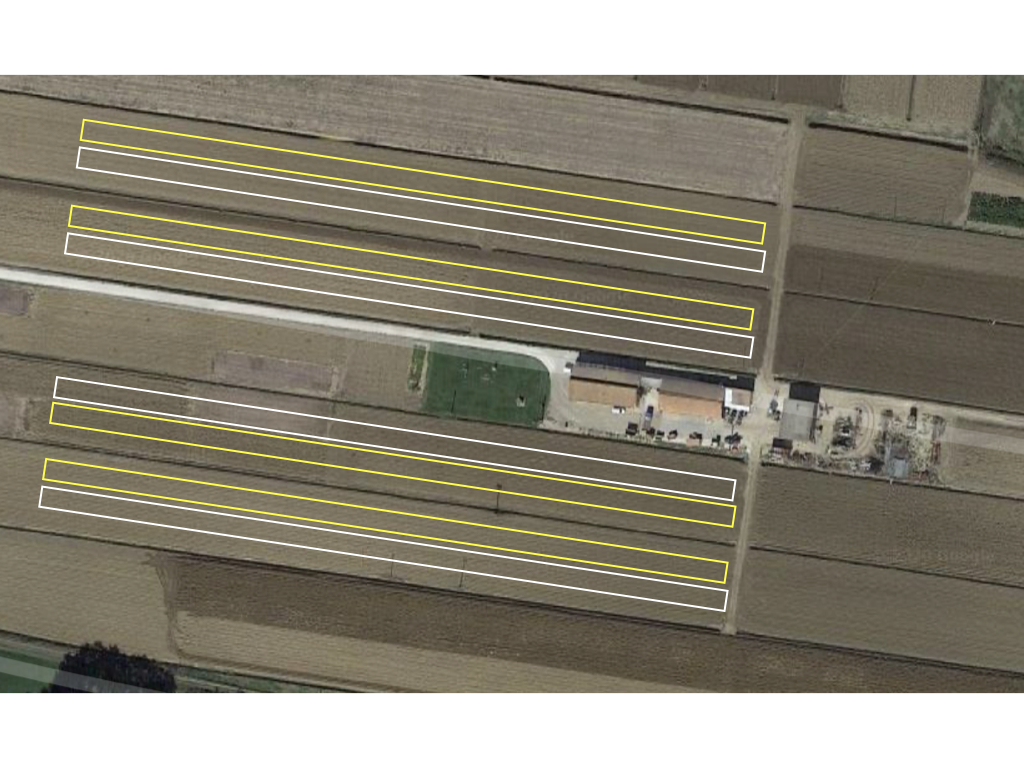
\includegraphics[width=0.9\linewidth]{_images/OnFarmTrial} 

}

\caption{Esempio di disegno sperimentale per una prova dimostrativa, con quattro campi, due strisce per campo e un diverso trattamento per striscia (giallo e bianco)}\label{fig:figName30a}
\end{figure}

Gli esperimenti dimostrativi sono spesso ripetuti nello spazio e nel tempo, per ottenere informazioni più attendibili sulla validità della tecnica innovativa.

Le prove parcellari sono, invece, una via di mezzo tra le prove dimostrative e gli esperimenti di laboratorio: pur essendo in pieno campo, le parcelle di terreno sono sufficientemente piccole per consentire un elevato grado di precisione e di controllo (Figura \ref{fig:figName21} ). Ovviamente, questo elevato grado di controllo consente di ottenere produzioni che sono, mediamente, un 10-30\% maggiori di quelle ottenibili su scala aziendale.

\begin{figure}

{\centering 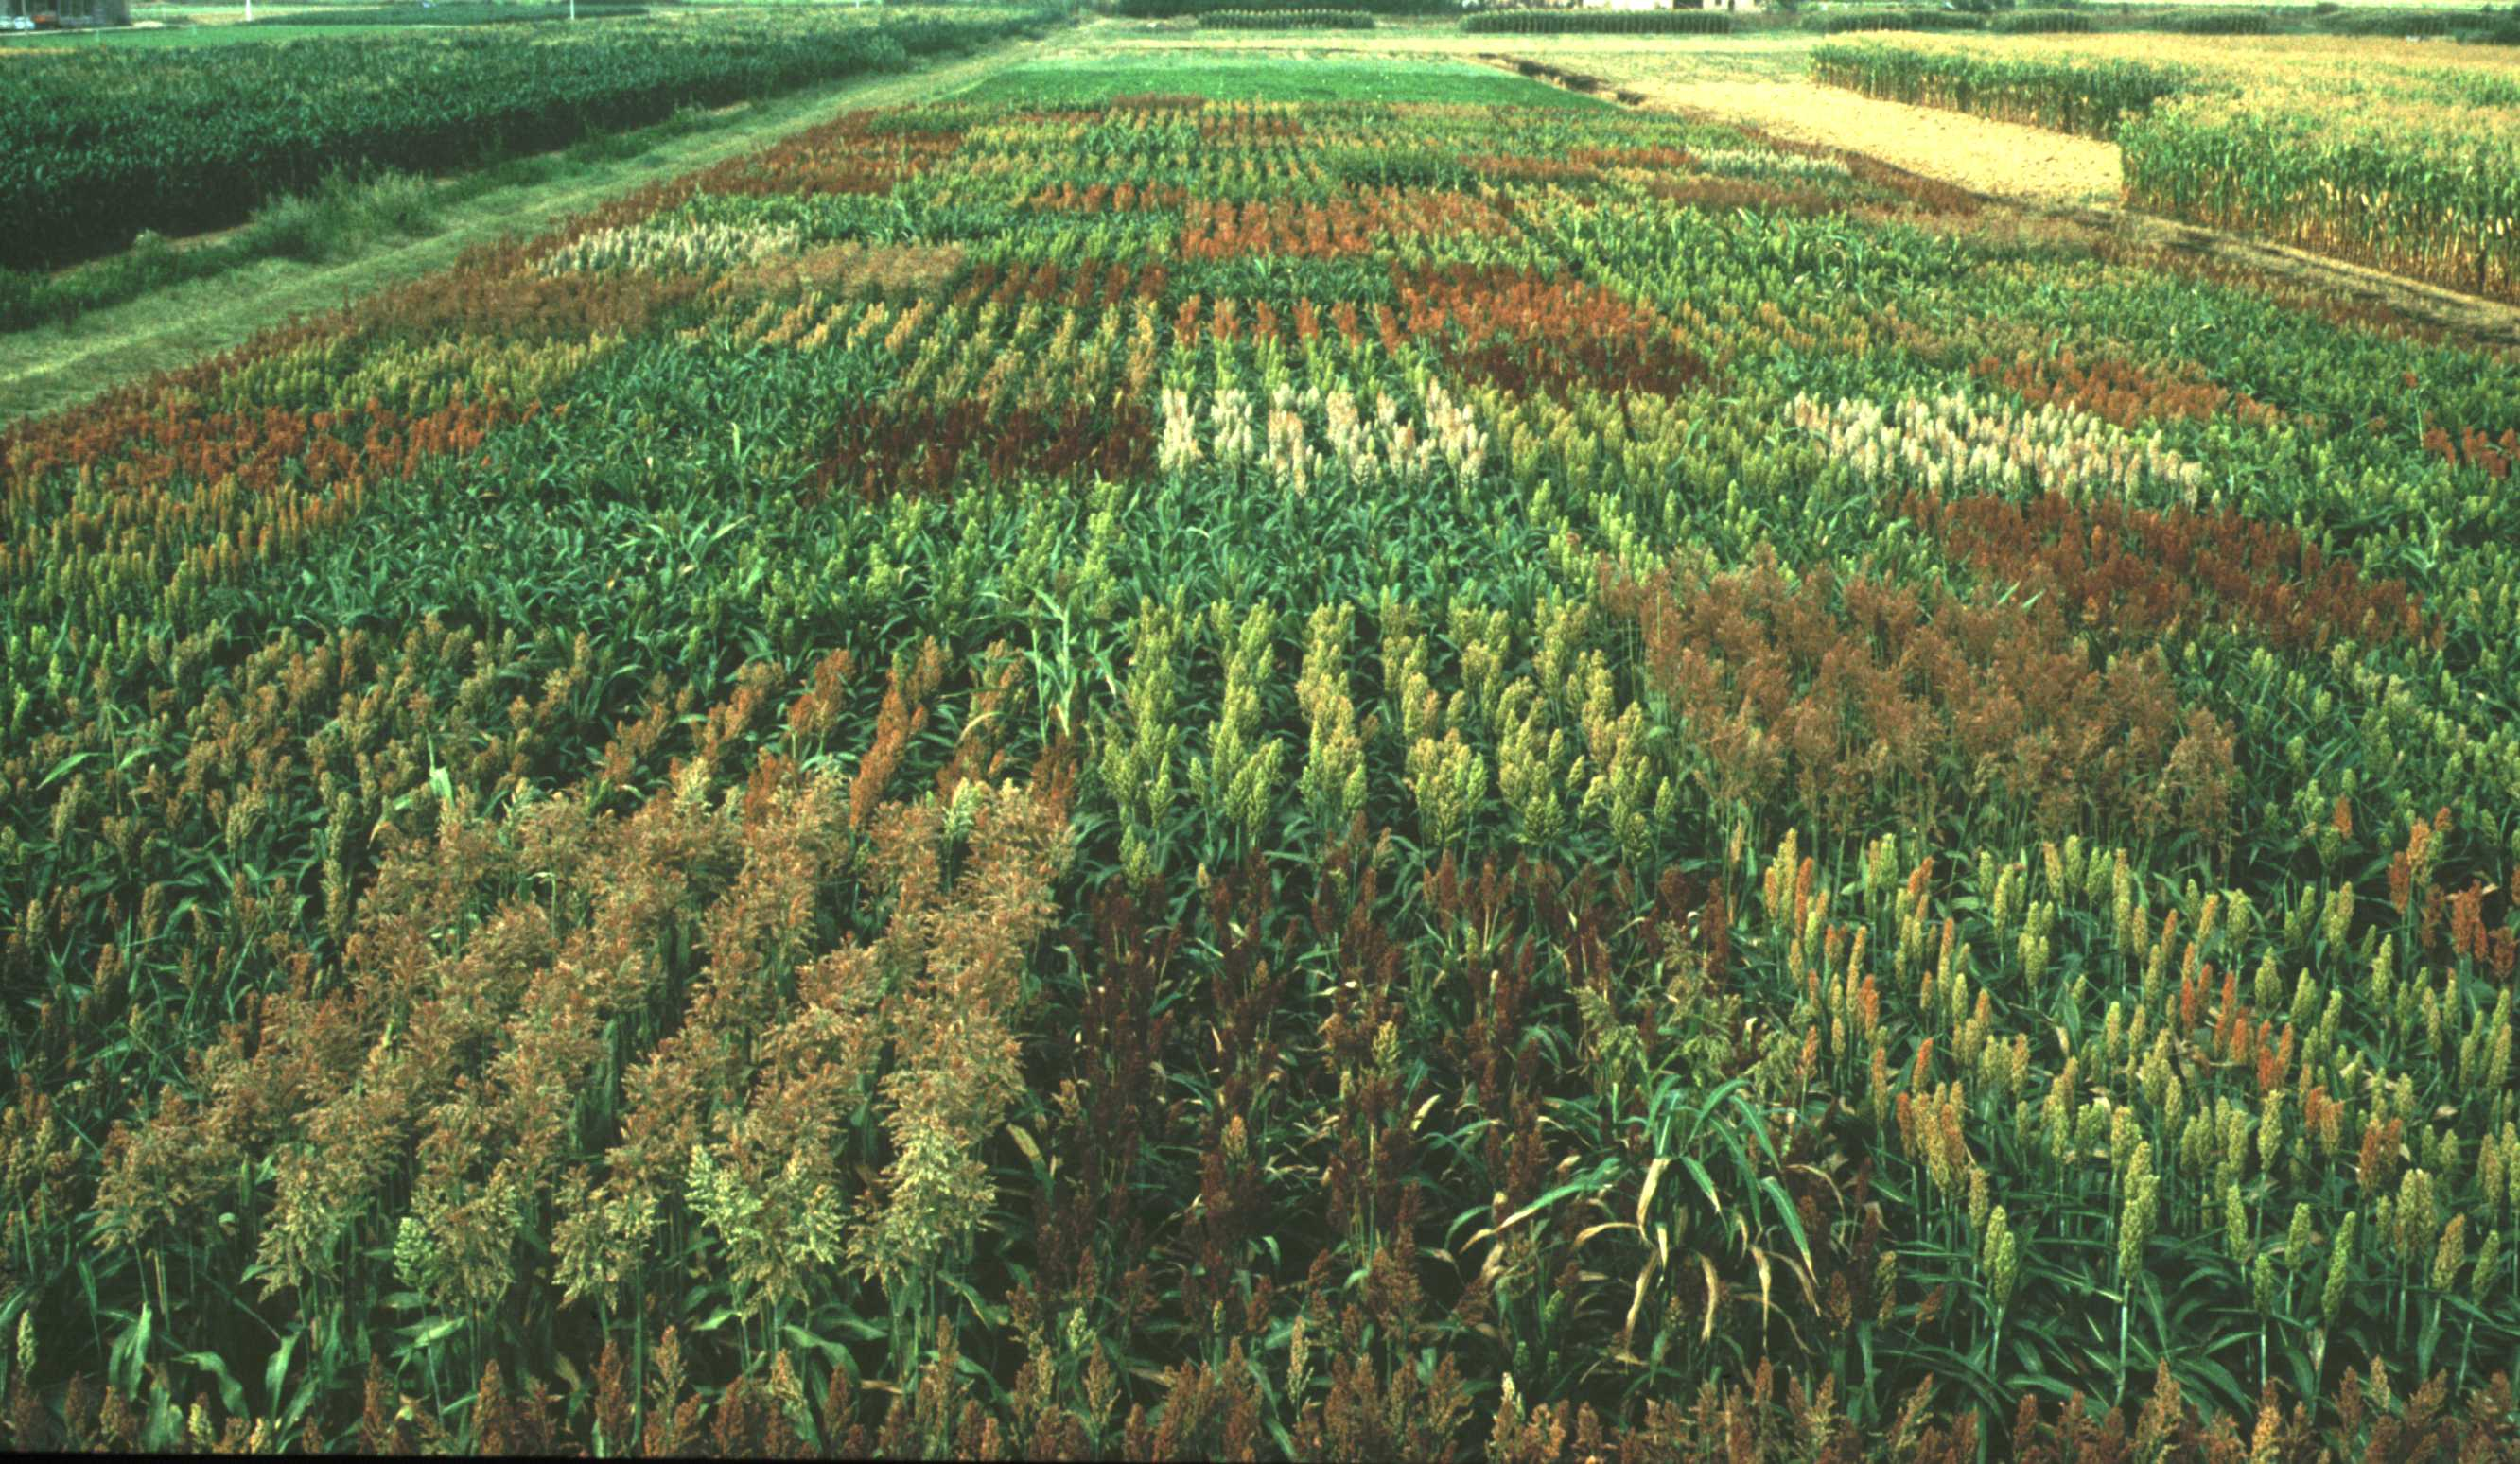
\includegraphics[width=0.9\linewidth]{_images/SorgoProveVarietali} 

}

\caption{Una prova sperimentale in campo (Foto D. Alberati)}\label{fig:figName21}
\end{figure}

La \textbf{dimensione delle parcelle} viene scelta in modo da avere un numero di piante sufficientemente alto da essere rappresentativo. Per questo motivo le colture a bassa fittezza (es. mais) hanno sempre bisogno di parcelle più grandi che non quelle ad alta fittezza (es. frumento). La dimensione non deve tuttavia essere troppo elevata, in quanto si viene a determinare un incremento della variabilità del terreno e, di conseguenza, una diminuzione della precisione dell'esperimento. Per questo motivo, talvolta si preferisce diminuire la dimensione delle parcelle ed, avendo lo spazio sufficiente, aumentare il numero delle repliche. E' poi importante tenere conto delle dimensioni delle macchine operatrici che verranno utilizzate per le pratiche colturali; in genere, la larghezza della parcella dovrebbe essere pari a un multiplo della larghezza di lavoro delle seminatrici e/o raccoglitrici e/o delle macchine per la distribuzione dei fitofarmaci.

Nello stabilire la dimensione delle parcelle, dovremo tener conto del fatto che la parte più delicata è il bordo, in quanto le piante che si trovano lungo di esso risentono di condizioni diverse dalle altre piante situate al centro della parcella (\textbf{effetto bordo}). Questo determina variabilità all'interno della parcella, che possiamo minimizzare raccogliendo solo la parte centrale. Si viene così a distinguere la superficie totale della parcella dalla superficie di raccolta (\textbf{superficie utile}), che può essere anche molto minore di quella totale.

Tenendo conto degli aspetti detti in precedenza, riteniamo che le colture ad elevata fittezza (frumento, cereali, erba medica\ldots) dovrebbero avere parcelle di almeno 10-20 m\textsuperscript{2}, mentre le colture a bassa fittezza (mais, girasole\ldots) dovrebbero avere parcelle di almeno 20-40 m\textsuperscript{2}, con riferimento alla superficie utile di raccolta.

Per quanto riguarda la \textbf{forma delle parcelle}, anche se il quadrato minimizzerebbe l'effetto bordo, perché, a parità di superficie, ha un perimetro più basso, nella pratica le parcelle sono sempre rettangolari, per facilitare l'esecuzione delle operazioni meccaniche.Come già detto, la larghezza dovrebbe essere pari ad un multiplo del fronte di lavoro delle macchine operatrici da impiegare.

\hypertarget{numero-di-repliche}{%
\subsection{Numero di repliche}\label{numero-di-repliche}}

Per gli esperimenti di pieno campo il numero di repliche oscilla tra tre e cinque; con meno repliche l'esperimento è inefficiente, mentre un numero più elevato di repliche può essere dannoso, in quanto aumenta la dimensione dell'esperimento e, con essa, la variabilità del campo. Inoltre, un numero alto di repliche aumenta i costi e i tempi di esecuzione dei rilievi. Il numero totale di parcella, alla fine, risulta dal prodotto tra il numero delle tesi sperimentali e il numero delle repliche.

\hypertarget{la-mappa-di-campo}{%
\subsection{La mappa di campo}\label{la-mappa-di-campo}}

Il disegno di un esperimento, di solito, è pianificato su una mappa. Un esempio è riportato in Figura \ref{fig:figName31}, relativamente ad un esperimento sistemato su un appezzamento largo 30 metri e lungo 400 metri. In questo caso abbiamo disegnato otto file di parcelle in senso trasversale (8 x 2.25 m = 18 m di larghezza), e quattro parcelle in senso longitudinale. Intorno all'esperimento abbiamo sistemato una serie di parcelle addizionali, con lo scopo di ridurre l'effetto `bordo'. Vediamo in figura che la mappa riporta tutte le informazioni che consentono di collocare correttamente l'esperimento nello spazio ed, inoltre, che le parcelle sono tutte chiaramente identificate con un codice numerico.

\begin{figure}

{\centering 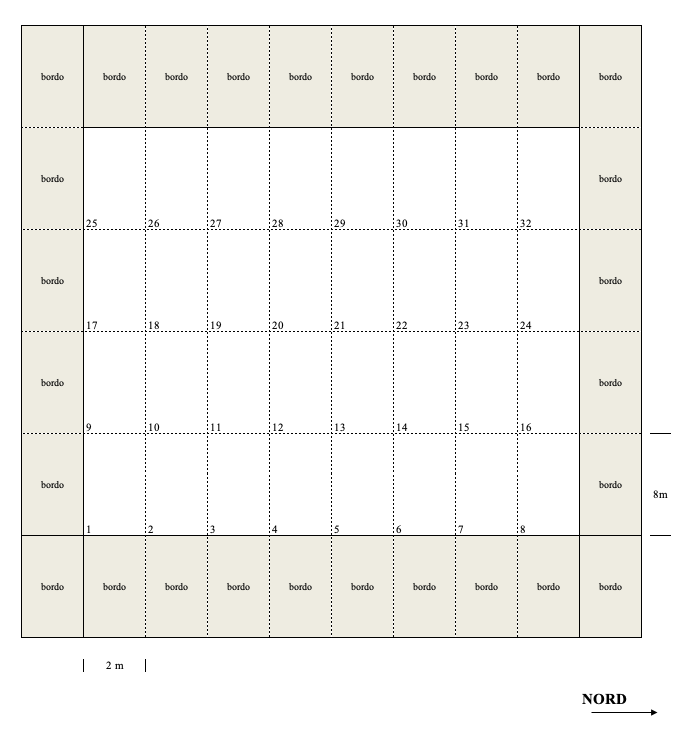
\includegraphics[width=0.9\linewidth]{_images/Mappa1} 

}

\caption{Mappa di campo di un esperimento con 32 parcelle}\label{fig:figName31}
\end{figure}

\hypertarget{lay-out-sperimentale}{%
\subsection{Lay-out sperimentale}\label{lay-out-sperimentale}}

Abbiamo già parlato di come possa essere conveniente, nella pratica sperimentale, porre dei vincoli alla randomizzazione. A seconda di come poniamo questi vincoli, distinguiamo diversi disegni sperimentali, che descriveremo nei prossimi paragrafi.

\hypertarget{disegni-completamente-randomizzati}{%
\subsubsection{Disegni completamente randomizzati}\label{disegni-completamente-randomizzati}}

Per queste prove, le più semplici, la scelta dei soggetti da trattare è totalmente casuale, senza vincoli di sorta. Il vantaggio principale è la semplicità; lo svantaggio sta nel fatto che tutte le eventuali differenze e disomogeneità tra unità sperimentali restano non riconosciute ed entrano nella definizione della variabilità residua. Per questo, i disegno completamente randomizzati sono utilizzato soprattutto per le situazioni di buona uniformità ambientale e tra i soggetti.

Come esempio, mostriamo un disegno completamente randomizzato utilizzando le parcelle della figura \ref{fig:figName31}, alle quali abbiamo allocato 8 trattamenti (da A ad H) con quattro repliche. Come si può notare, l'allocazione è completamente casuale (figura \ref{fig:figName33})

\begin{figure}

{\centering 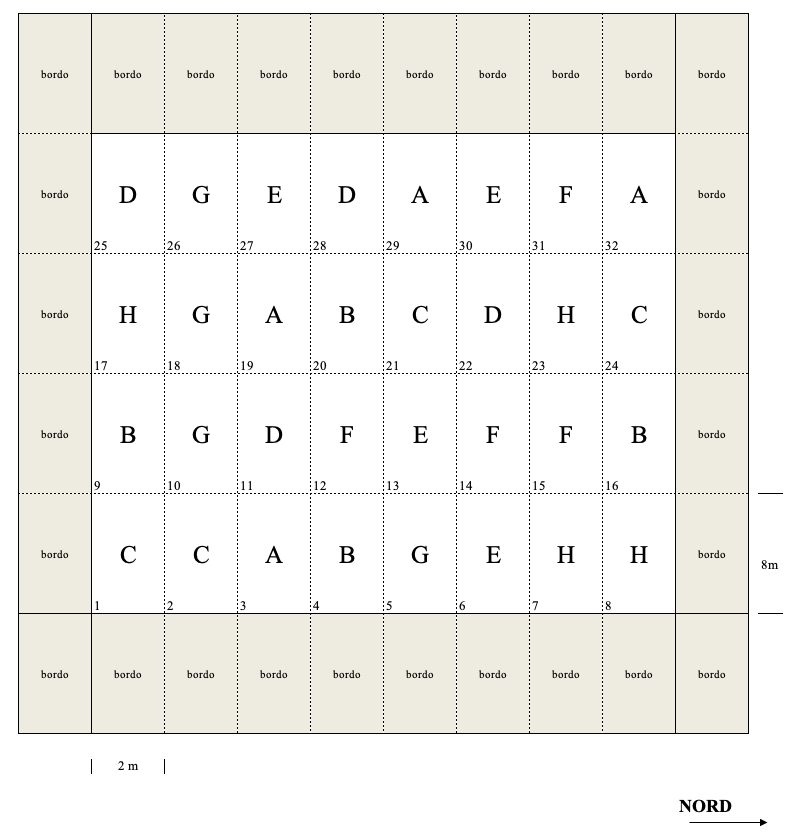
\includegraphics[width=0.9\linewidth]{_images/Mappa1CRD} 

}

\caption{Esempio di uno schema sperimentale a randomizzazione completa}\label{fig:figName33}
\end{figure}

\hypertarget{disegni-a-blocchi-randomizzati}{%
\subsubsection{Disegni a blocchi randomizzati}\label{disegni-a-blocchi-randomizzati}}

Quando le unità sperimentali non sono totalmente omogenee, ma vi è una certa variabilità per una qualche caratteristiche rilevante, potremo dividere i soggetti in base a questa caratteristica, in tanti gruppi quante sono le repliche.

Ad esempio, nel caso dello schema in figura \ref{fig:figName33}, se ammettiamo l'esistenza di un gradiente di fertilità crescente das sinistra verso destra, allora il trattamento H è stato avvantaggiato, perché tre delle quattro repliche si trovano nella parte destra, mentre il trattamento G è stato svantaggiato, per il motivo opposto.

Si può ottenere un disegno più efficiente se dividendo l'esperimento in quattro blocchi perpendicolari al gradiente di fertilità. Ad esempio il blocco 1 conterrà le parcelle 1, 9, 17, 25, 2, 10, 18 e 26, cioè le prime due colonne della mappa, con un numero di parcelle esattamente uguali al numero dei trattamenti. Il blocco 2 conterrà le colonne 3 e 4 e così via. Dato che il gradiente è trasversale, le parcelle di un stesso blocco saranno più omogenee che non parcelle su blocchi diversi. Dopo aver diviso la mappa in quattro blocchi di otto parcelle, potremo allocare gli otto trattamenti a random all'interno di ogni blocco (\ref{fig:figName34})

\begin{figure}

{\centering 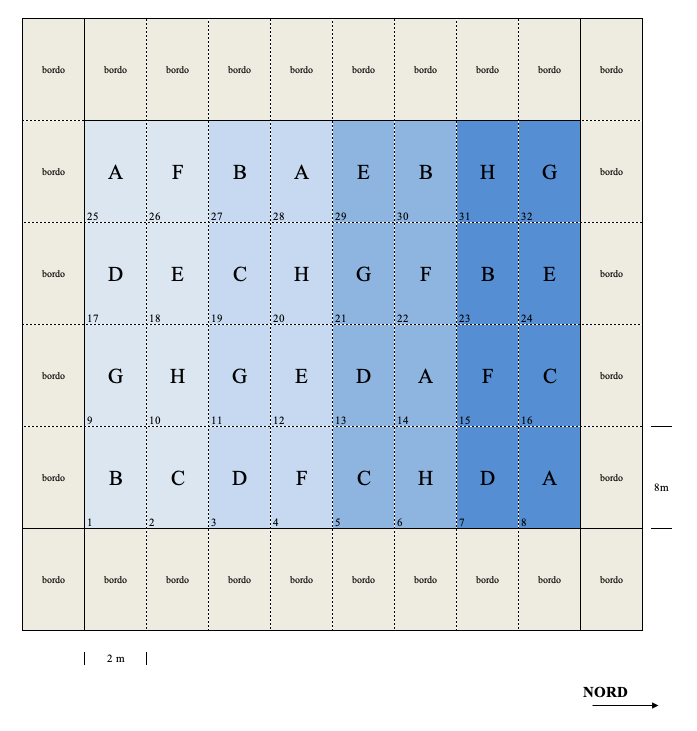
\includegraphics[width=0.9\linewidth]{_images/Mappa1CRBD} 

}

\caption{Esempio di uno schema sperimentale a blocchi randomizzati}\label{fig:figName34}
\end{figure}

Un disegno a blocchi randomizzati non è solo tipico della sperimentazione di campo. Ad esempio, volendo determinare la contaminazione da micotossine nelle confezioni di datteri, a seconda della modalità di confezionamento (es. carta, busta di plastica, scatola di plastica perforata), si può sospettare che il supermercato nel quale le confezioni vengono vendute potrebbe avere un certo effetto, legato alle modalità di conservazione. Per cui, invece che prelevare trenta confezioni (dieci per metodo) a caso nei supermercati di una città, scegliamo dieci supermercati e, in ognuno, prendiamo una confezione per tipo. In questo caso, il supermercato fa da blocco.

Il vantaggio del disegno a blocchi randomizzati sta nel fatto che ci permetto di utilizzare soggetti sperimentali con una più bassa omogeneità iniziale, aspetto importante quando il numero di unità sperimentali richieste comincia ad essere elevato. Infatti, le differenze tra soggetti sperimentali, almeno in parte, possono essere spiegate attraverso l'appartenenza ad un determinato gruppo (blocco) e possono quindi essere scorporate dal calcolo della variabilità residua.

\hypertarget{disegni-a-quadrato-latino}{%
\subsubsection{Disegni a quadrato latino}\label{disegni-a-quadrato-latino}}

In questo caso, le unità sperimentali presentano due `gradienti', cioè vi sono differenze legate a due elementi importanti, oltre al trattamento sperimentale. La Figura \ref{fig:figName35} mostra un esperimento con quattro trattamenti e altrettante repliche, nel quale ogni trattamento si trova in tutte le righe e tutte le colonne, in modo da poter considerare eventuali gradienti di fertilità da destra verso sinistra e dall'alto verso il basso. La figura mostra anche perché si parli di quadrato latino: in effetti il numero di righe è uguale al numero di colonne, secondo una griglia quadrata. Qualcuno di voi riconoscerà in questo schema i principi di fondo del Sudoku.

\begin{figure}

{\centering 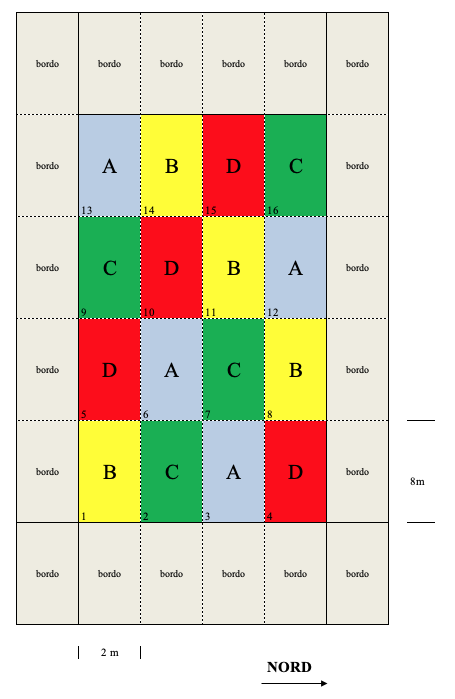
\includegraphics[width=0.7\linewidth]{_images/Mappa2LS} 

}

\caption{Esempio di un disegno sperimentale a quadrato latino, con quattro trattamenti (A, B, C e D) ed altrettante repliche. I colri aiutano ad identificare i quattro trattamenti e la posizione delle rispettive parcelle}\label{fig:figName35}
\end{figure}

I disegni a quadrato latino non sono solo utili per gli esperimenti di pieno campo; ad esempio, se un certo oggetto richiede un solo operatore per essere costruito e vogliamo confrontare quattro metodi costruttivi, possiamo pianificare un esperimento dove l'unità sperimentale è il lavoratore. Volendo lavorare con quattro repliche, avremmo bisogno di sedici operatori per disegnare un esperimento completamente randomizzato. Possiamo tuttavia considerare che un operatore, in quattro turni successivi, può operare con tutti e quattro i metodi. Quindi possiamo disegnare un esperimento in cui il turno fa da unità sperimentale e l'operatore fa da blocco (esperimento a blocchi randomizzati).

Tuttavia, in ogni blocco (operatore) vi è un gradiente, nel senso che i turni successivi al primo sono via via meno efficienti, perché l'operatore accumula stanchezza. Per tener conto di questo, potremmo lasciare all'operatore un congruo periodo di tempo tra un turno e l'altro. Oppure, potremmo introdurre un vincolo ulteriore, per ogni operatore, randomizzando i quattro metodi tra i turni, in modo che ogni metodo, in operatori diversi, capiti in tutti i turni. In sostanza, l'operatore fa da blocco, perché in esso sono contenuti tutti i metodi. Ma anche il turno (per tutti gli operatori) fa da blocco, in quanto in esso sono ancora contenuti tutti i metodi. Proviamo a schematizzare, nella figura seguente (\ref{fig:figName391} ).

\begin{figure}

{\centering 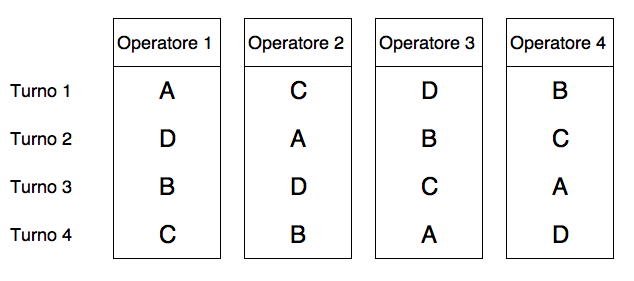
\includegraphics[width=0.9\linewidth]{_images/TurniOperatori} 

}

\caption{Allocazione di quattro metodi di lavoro (A, B, C e D), tra quattro operatori, in quattro turni, seguendo uno schema a quadrato latino}\label{fig:figName391}
\end{figure}

Il disegno a quadrato latino è utile, perché possiamo dar conto sia delle differenza tra righe (es. turni), che delle differenze tra colonne (es. operatori), in modo da ridurre al minimo possibile la variabilità inspiegabile. Lo svantaggio sta nel fatto che, dovendo avere tante repliche quanti sono i trattamenti, è utilizzabile solo per esperimenti abbastanza piccoli.

\hypertarget{disegni-a-split-plot}{%
\subsubsection{Disegni a split-plot}\label{disegni-a-split-plot}}

Gli esperimenti fattoriali possono essere disegnati con uno schema a randomizzazione completa o a blocchi randomizzati, allocando alle unità sperimentali tutte le combinazioni dei fattori in studio. Per esempio, consideriamo un esperimento per confrontare tre tipi di lavorazioni del terreno (minimum tillage = MIN; aratura superficiale = SP; aratura profonda = DP) e due tipi di controllo chimico delle piante infestanti (a pieno campo = TOT; lungo la fila = PARZ). Se vogliamo fare quattro repliche, i sei trattamenti sperimentali (MIN-TOT, SP-TOT, DP-TOT, MIN-PARZ, SP-PARZ and DP-PARZ) possono essere allocati alle 24 parcelle secondo uno schema a blocchi randomizzati, come indicato in Figura \ref{fig:figName37}. In questo caso è necessario lasciare un ampio spazio tra le parcelle, in modo da permettere la circolazione delle macchine operatrici per la lavorazione ed, inoltre, le parcelle debbono essere grandi, per consentire una buona esecuzione dell'aratura.

\begin{figure}

{\centering 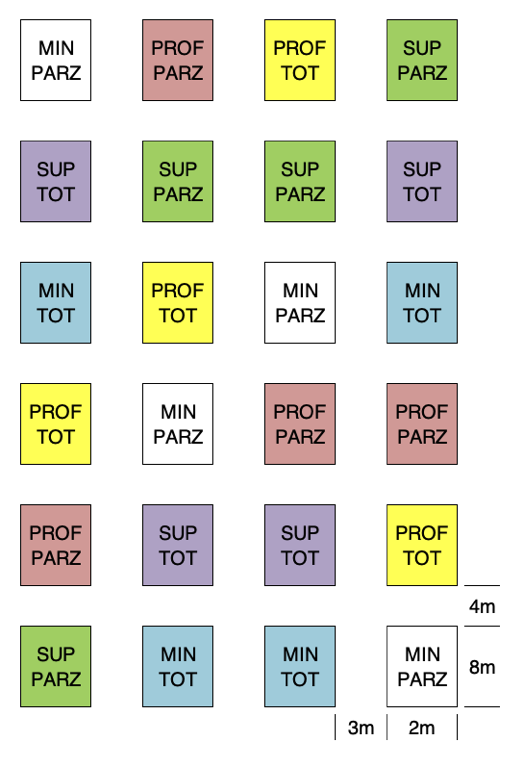
\includegraphics[width=0.75\linewidth]{_images/Mappa3FATT} 

}

\caption{Mappa di campo per un esperimento fattoriale con due fattori, disegnato a blocchi randomizzati}\label{fig:figName37}
\end{figure}

Dato che il trattamento di diserbo non richiede parcelle altrettanto grosse, potremmo pensare di suddividere ogni parcella in due sub-parcelle, sulle quali allocare il trattamento di diserbo (disegno a \textbf{parcella suddivisa} o \textbf{split-plot}). Un esempio è riportato in Figura \ref{fig:figName38}, dove possiamo osservare che le lavorazioni sono allocate su 12 parcelle principali (mainplots), secondo uno schema a blocchi randomizzati, mentre i trattamenti di diserbo sono allocati in modo randomizzato sulle due subplot in ogni mainplot. Tecnicamente, diciamo che la lavorazione è il fattore di primo ordine, mentre il diserbo chimico è il fattore di secondo ordine. Notiamo che l'esperimento diviene più piccolo e quindi più preciso.

\begin{figure}

{\centering 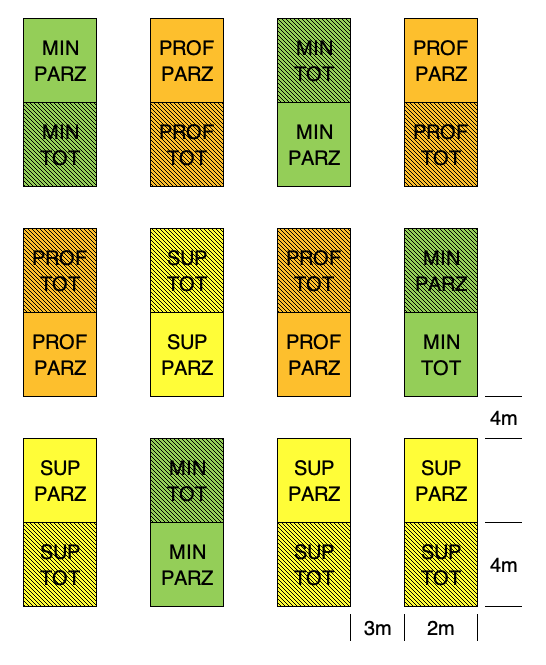
\includegraphics[width=0.75\linewidth]{_images/Mappa3split} 

}

\caption{Stesso esperimento descritto nella figura precedente, ma disegnato con uno schema a split-plot.}\label{fig:figName38}
\end{figure}

In generale, un disegno a split-plot può rendersi necessario per i seguenti motivi:

\begin{enumerate}
\def\labelenumi{\arabic{enumi}.}
\tightlist
\item
  un fattore sperimentale richiede parcelle più grandi dell'altro. Di conseguenza si disegna l'esperimento per il fattore che richiede parcelle più grandi, che vengono poi suddivise per accomodare l'altro fattore sperimentale.
\item
  Uno dei due fattori sperimentali è più `difficile' da assegnare rispetto all'altro e quindi è preferibile manipolare congiuntamente tutto il gruppo di unità sperimentali che deve riceverlo. Ad esempio, se vogliamo misurare la resistenza alla corrosione di barre d'acciaio con diversi rivestimenti e forgiate a diverse temperature, è evidente che la gestione della temperatura nella fornace è piuttosto complessa, perché richiede tempi lunghi per essere cambiata e raggiungere un nuovo equilibrio. Invece che preparare una fornace per ogni rivestimento (manipolazione indipendente delle unità sperimentali), si mettono nella stessa fornace tutte le unità sperimentali con i diversi rivestimenti. Una situazione analoga si può avere se vogliamo provare diverse miscele per torte (con vari ingredienti), e diversi tempi di cottura; dato che non è agevole preparare una miscela diversa per ogni tempo di cottura, potremmo preparare una miscela tutta insieme, per poi suddividerla tra i diversi tempi di cottura.
\item
  La disponibilità di unità sperimentali è limitata, come accade con gli armadi climatici, che vengono impostati a diversa temperatura e all'interno delle quali vengono randomizzate le tesi sperimentali di secondo ordine.
\end{enumerate}

Un'importante conseguenza dei disegni a split-plot è che ogni mainplot funge da replica per il fattore sperimentale di secondo ordine. In effetti, se guardiamo alla Figura \ref{fig:figName38}, possiamo osservare che ci sono quattro repliche per ogni lavorazione, ma 12 repliche per ogni tipo di diserbo chimico. Di conseguenza, l'effetto del fattore sperimentale di secondo ordine è stimato con maggior precisione.

\hypertarget{disegni-a-strip-plot}{%
\subsubsection{Disegni a strip-plot}\label{disegni-a-strip-plot}}

In alcune circostanze, soprattutto nelle prove di diserbo chimico, potrebbe trovare applicazione un altro tipo di schema sperimentale, nel quale ogni blocco viene diviso in tante righe quanti sono i livelli di un fattore sperimentale e tante colonne quanti sono i livelli dell'altro. In questo modo, il primo trattamento sperimentale viene applicato a tutte le parcelle di una riga e l'altro trattamento a tutte le parcelle di una colonna. Ovviamente, l'allocazione alle righe e alle colonne è casuale e cambia in ogni blocco.

Questo disegno è detto \textbf{strip-plot} ed è molto comodo perché consente di lavorare velocemente. Se consideriamo il caso studio precedente, un disegno a strip-plot potrebbe essere immaginato come in Figura \ref{fig:figName253}.

\begin{figure}

{\centering 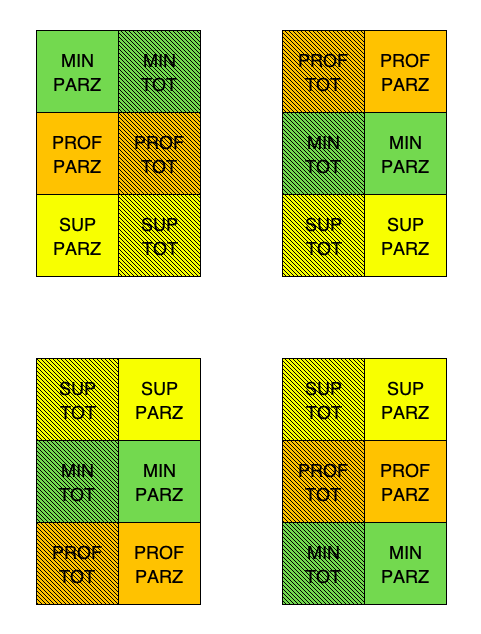
\includegraphics[width=0.7\linewidth]{_images/Mappa3Strip} 

}

\caption{Esempio di un disegno a strip-plot per il dataset 'beet.csv', che prevede tre livelli di lavorazione e due livelli di diserbo chimico}\label{fig:figName253}
\end{figure}

\begin{center}\rule{0.5\linewidth}{0.5pt}\end{center}

\hypertarget{altre-letture-1}{%
\section{Altre letture}\label{altre-letture-1}}

\begin{enumerate}
\def\labelenumi{\arabic{enumi}.}
\tightlist
\item
  Cochran, W.G., Cox, G.M., 1950. Experimental design. John Wiley \& Sons, Inc., Books.
\item
  LeClerg, E.L., Leonard, W.H., Clark, A.G., 1962. Field Plot Technique. Burgess Publishing Company, Books.
\end{enumerate}

\hypertarget{domande-ed-esercizi}{%
\section{Domande ed esercizi}\label{domande-ed-esercizi}}

\hypertarget{domanda-1}{%
\subsection{Domanda 1}\label{domanda-1}}

Quali sono le caratteristiche fondamentali di un esperimento scientifico, perché possa essere ritenuto valido?

\hypertarget{domanda-2}{%
\subsection{Domanda 2}\label{domanda-2}}

Illustrare brevemente il metodo scientifico `galileiano'.

\hypertarget{domanda-3}{%
\subsection{Domanda 3}\label{domanda-3}}

Illustrare brevemente la differenza tra errori casuali e sistematici. In presenza di quale dei due è possibile ottenere risultati scientifici validi?

\hypertarget{domanda-4}{%
\subsection{Domanda 4}\label{domanda-4}}

Qual è la differenza tra repliche vere e pseudo-repliche?

\hypertarget{domanda-5}{%
\subsection{Domanda 5}\label{domanda-5}}

Cosa è il confounding e come può rendere distorti i risultati di un esperimento scientifico?

\hypertarget{domanda-6}{%
\subsection{Domanda 6}\label{domanda-6}}

Quali sono gli elementi comuni a tutti gli esperimenti scientifici?

\hypertarget{domanda-7}{%
\subsection{Domanda 7}\label{domanda-7}}

Quali tipi di variabili conoscete e quali sono le loro caratteristiche?

\hypertarget{domanda-8}{%
\subsection{Domanda 8}\label{domanda-8}}

Qual è la differenza tra un esperimento fattoriale innestato ed uno incrociato

\hypertarget{domanda-9}{%
\subsection{Domanda 9}\label{domanda-9}}

Quali sono le caratteristiche principali degli esperimenti a randomizzazione completa, blocchi randomizzati e quadrato latino?

\hypertarget{domanda-10}{%
\subsection{Domanda 10}\label{domanda-10}}

Come è fatto e quando si utilizza uno schema sperimentale a split-plot?

\hypertarget{domanda-12}{%
\subsection{Domanda 12}\label{domanda-12}}

Cosa è l'effetto di bordo e come si può controllare?

\hypertarget{domanda-13}{%
\subsection{Domanda 13}\label{domanda-13}}

Illustrare e discutere le caratteristiche fondamentali delle `parcelle' (forma, dimensioni, numero \ldots)

\hypertarget{esercizio-1}{%
\subsection{Esercizio 1}\label{esercizio-1}}

Vi è stata affidata una prova sperimentale per la taratura agronomica di un nuovo diserbante appartenente al gruppo chimico delle solfoniluree (AGRISULFURON), utilizzabile alla dose presumibile di 20 g/ha, per il diserbo di post-emergenza del mais. Gli obiettivi della prova sono:

\begin{enumerate}
\def\labelenumi{\arabic{enumi}.}
\tightlist
\item
  Valutare se è opportuno un certo aggiustamento della dose (incremento/diminuzione)
\item
  Valutare se è opportuna l'aggiunta di un bagnante non-ionico
\item
  Valutare se è opportuno splittare la dose di 20 g/ha in due distribuzioni
\item
  Valutare l'efficacia del nuovo diserbante con gli opportuni controlli (testimoni)
\end{enumerate}

Coerentemente con questi obiettivi, scrivere un protocollo sperimentale sufficientemente dettagliato (una pagina) ed aggiungere la mappa di campo della prova. Considerare che abbiamo a disposizione un campo lungo 80 metri e largo 26 metri, in direzione Nord-Sud, lavorato nel senso della lunghezza e con un gradiente di `fertilità' trasversale, nel senso della larghezza.

\hypertarget{esercizio-2}{%
\subsection{Esercizio 2}\label{esercizio-2}}

Dovete progettare una prova sperimentale per valutare i possibili effetti dell'epoca di semina (autunnale oppure primaverile) su sette varietà di favino (che etichetteremo con le lettere da A a G). Progettare un esperimento di pieno campo, decidendo il numero di repliche ed il lay-out sperimentale. Redigere la mappa di campo ed allocare i trattamenti, in base al lay-out prescelto. Aggiungere alla mappa di campo tutti i dettagli necessari (dimensioni delle parcelle, localizzazione ed orientamento dell'esperimento). Considerate che abbiamo a disposizione un campo lungo 60 metri e largo 40 metri, in direzione Est-Ovest, lavorato nel senso della lunghezza e con un gradiente di `fertilità' longitudinale.

\hypertarget{esercizio-3}{%
\subsection{Esercizio 3}\label{esercizio-3}}

Illustrate il disegno sperimentale che adottereste per organizzare una prova che metta a confronto quattro concimi azotati (urea, solfato ammonico, nitrato di calcio e nitrato di sodio) e un testimone non concimato su barbabietola da zucchero. Motivate opportunamente le vostre scelte. Considerate che abbiamo a disposizione un campo lungo 50 metri e largo 30 metri, in direzione Est-Ovest, lavorato nel senso della lunghezza e con due gradienti di `fertilità', longitudinale e trasversale.

\hypertarget{esercizio-4}{%
\subsection{Esercizio 4}\label{esercizio-4}}

Descrivete lo schema sperimentale che adottereste per organizzare un esperimento di confronto tra quattro dosi di un diserbate per il frumento, utilizzato con e senza un coadiuvante. Motivate opportunamente le vostre scelte. Considerate che abbiamo a disposizione un campo lungo 50 metri e largo 20 metri, in direzione Est-Ovest, lavorato nel senso della lunghezza e con due gradienti di `fertilità', longitudinale e trasversale.

\hypertarget{esercizio-5}{%
\subsection{Esercizio 5}\label{esercizio-5}}

Descrivete lo schema sperimentale che utilizzereste per organizzare una prova su pomodoro da industria, per la valutazione dell'effetto di tre livelli di concimazione azotata (0, 80 e 160 kg/ha) e tre tipologie di interventi irrigui (asciutto, basso volume irriguo, alto volume irriguo). Motivate opportunamente le vostre scelte. Considerate che abbiamo a disposizione un campo lungo 100 metri e largo 25 metri, in direzione Est-Ovest, lavorato nel senso della lunghezza e con un gradiente di fertilità longitudinale.

\hypertarget{richiami-di-statistica-descrittiva}{%
\chapter{Richiami di statistica descrittiva}\label{richiami-di-statistica-descrittiva}}

Qualunque esperimento include un processo di raccolta dati, tramite osservazioni e/o misurazioni, al termine del quale abbiamo a disposizione un collettivo di valori, di solito organizzati sotto forma di tabella (`dataset'), dove ogni riga corrisponde ad un'unità sperimentale (soggetto) con tutti i suoi attributi, mentre ogni colonna (detta anche variabile) corrisponde ad un attributo e contiene i valori rilevati per tutte le unità sperimentali. Un esempio delle prime righe di un dataset è riportato nella Tabella \ref{tab:tabName1}.

\begin{table}

\caption{\label{tab:tabName1}Prime 6 righe di un dataset relativo alla qualità di alcuni genotipi di frumento. Ogni riga rappresenta un'unità sperimentale ed ogni colonna rappresenta un attributo di quella unità sperimentale (TKW: peso dei mille semi in grammi; Whectol: peso ettolitrico in kg; Yield: produzione di granella in quintali per ettaro; height: altezza in cm.)}
\centering
\begin{tabular}[t]{l|r|r|r|r|r}
\hline
Genotype & Block & Height & TKW & Whectol & Yield\\
\hline
arcobaleno & 1 & 90 & 44.5 & 83.2 & 64.40\\
\hline
arcobaleno & 2 & 90 & 42.8 & 82.2 & 60.58\\
\hline
arcobaleno & 3 & 88 & 42.7 & 83.1 & 59.42\\
\hline
baio & 1 & 80 & 40.6 & 81.8 & 51.93\\
\hline
baio & 2 & 75 & 42.7 & 81.3 & 51.34\\
\hline
baio & 3 & 76 & 41.1 & 81.1 & 47.78\\
\hline
\end{tabular}
\end{table}

Il nostro primo compito è quello di comprendere e descrivere le caratteristiche fondamentali di ogni variabile, utilizzando statistiche descrittive opportunamente scelte, in base al tipo di dato e alle caratteristiche che si vogliono descrivere.

\hypertarget{descrizione-di-dati-quantitativi}{%
\section{Descrizione di dati quantitativi}\label{descrizione-di-dati-quantitativi}}

Se i dati sono stati ottenuti con un processo di misurazione e rappresentano una quantità, come, ad esempio, il peso, l'altezza, la concentrazione e così via, abbiamo una variabile quantitativa, della quale dobbiamo descrivere almeno due caratteristiche fondamentali:

\begin{enumerate}
\def\labelenumi{\arabic{enumi}.}
\tightlist
\item
  tendenza centrale
\item
  dispersione
\end{enumerate}

La tendenza centrale è un valore che rappresenta il `centro', attorno al quale si collocano tutte le osservazioni; al contrario, la dispersione misura la distanza delle osservazioni tra di loro, cioè, in altre parole, la loro variabilità. Ovviamente, esistono anche altre importanti proprietà di una variabile quantitativa, come la simmetria e la curtosi, che, tuttavia, non verranno prese in considerazione in questo libro, rimandando alla lettura di testi più approfonditi (Sokal e Rohlf, 1981; Leti e Cerbara, 2009).

Un altro aspetto che è necessario precisare è che, almeno nella sperimentazione agraria, non è infrequente rilevare, in ogni parcella, alcune variabili nominali, come la presenza di individui infetti la presenza/assenza di piante infestanti oppure alcune variabili discrete, frutto di conteggio, ad esempio il numero di piante infestanti o la fittezza della coltura e così via. Nonostante esistano metodi specifici per variabili nominali e discrete, è comune trasformare le variabili nominali in forma di frequenze relative (ad esempio, il numero di piante infette sul totale campionato) per ogni parcella, che sono poi trattate alla stregua delle variabili quantitative, così come i conteggi per parcella.

\hypertarget{indicatori-di-tendenza-centrale}{%
\subsection{Indicatori di tendenza centrale}\label{indicatori-di-tendenza-centrale}}

L'indicatore di tendenza centrale più diffuso è la \emph{media} aritmetica, che non necessita di particolari spiegazioni: si tratta della somma dei dati (\(x\)) divisa per il loro numero (\(n\)):

\[\mu = \frac{\sum\limits_{i = 1}^n x}{n}\]

Per esempio, consideriamo il seguente dataset, che elenca le altezze di quattro piante di mais \(d = [178, 175, 158, 153]\)

Il calcolo della media è banale:

\[\mu = \frac{178 + 175 + 158 + 153}{4} = 166\]

La media è `centrale' nel senso che la somma delle sue distanze da ogni altra osservazione è nulla. Di conseguenza, è molto sensibile ai valori estremi; se, ad esempio, supponiamo di avere i cinque valori: 1, 4, 7, 9 e 10 con media pari a 6,2 e supponiamo di sostituire il valore più alto con 100, la media aumenta di conseguenza, diventando pari a 24,2. Per questa sua sensibilità ai valori estremi, si dice che la media non è un indicatore di tendenza centrale `robusto' nei confronti degli \emph{outliers}, cioè delle osservazioni in qualche modo `aberranti'. In presenza di queste osservazioni, che potrebbero essere frutto di un errore sperimentale rilevante, la media tende a non rappresentare più la tendenza centrale del collettivo in modo affidabile.

Un altro indicatore di tendenza centrale è la \emph{mediana}, cioè il valore che bipartisce i dati in modo che la metà di essi siano più alti e la metà più bassi. Per calcolare la mediana, basta ordinare i soggetti in ordine crescente: se il numero di individui è dispari, la mediana è data dal valore dall'individuo che occupa il posto centrale o, se gli individui sono in numero pari, dalla media delle due osservazioni centrali. Nell'esempio precedente, i dati sono in numero pari, quindi la mediana è: \((158 + 175)/2 = 166.5\).

La mediana è un indicatore più robusto della media: infatti, se consideriamo gli stessi cinque valori elencati in precedenza (1, 4, 7, 9 e 10), la mediana è pari a 7 e non cambia quando sostituiamo il valore più alto con 100.

\hypertarget{indicatori-di-dispersione}{%
\subsection{Indicatori di dispersione}\label{indicatori-di-dispersione}}

Conoscere la tendenza centrale di un collettivo è importante, ma non è sufficiente. Infatti, una media pari a 100 può essere ottenuta con tre individui che misurano 99, 100 e 101, rispettivamente, o con tre individui che misurano 1, 100 e 199. E' evidente che i due gruppi hanno la stessa tendenza centrale, ma sono molto diversi in termini di dispersione (o variabilità) rispetto alla media. Per descrivere la dispersione dei dati possiamo utilizzare il \emph{campo di variazione}, che è la differenza tra la misura più bassa e la misura più alta. In realtà, questo indicatore è poco diffuso, perché considera solo i valori estremi del collettivo e non necessariamente cresce al crescere della variabilità. Altri indicatori sono più diffusi ed affidabili, come la devianza, la varianza, la deviazione standard ed il coefficiente di variabilità, tutti legati da relazioni algebriche ben definite.

La \emph{devianza}, generalmente nota come somma dei quadrati (abbreviata SS, da \emph{sum of squares}) è data da:

\[SS = \sum\limits_{i = 1}^n {(x_i  - \mu)^2 }\]

Ad esempio, per le quattro altezze menzionate in precedenza, la devianza è pari a:

\[SS = \left(178 - 166 \right)^2 + \left(175 - 166 \right)^2 + \left(158 - 166 \right)^2  + \left(153 - 166 \right)^2 = 458\]

La devianza è un indicatore di dispersione molto utilizzato, soprattutto perché ha un suo preciso significato geometrico, in quanto somma delle distanze euclidee al quadrato, rispetto alla media. Tuttavia, ha due aspetti che vanno tenuti in considerazione: in primo luogo, proprio perché è una somma, il valore finale dipende dal numero di addendi e quindi non la si può utilizzare per confrontare la variabilità di collettivi con diversa numerosità. Inoltre, l'unità di misura della devianza è pari al quadrato dell'unità di misura originale dei dati; ad esempio se le osservazioni sono espresse in centimetri (come nel nostro esempio), la devianza è espressa in centimetri quadrati, il che rende più difficoltosa l'interpretazione dei risultati.

Oltre dalla devianza, un indicatore molto utilizzato è la \emph{varianza campionaria} (o semplicemente \emph{varianza}), che è data dalla devianza divisa per il numero di dati meno uno:

\[\sigma^2  = \frac{SS}{n - 1}\]

Nel caso delle nostre altezze:

\[\sigma^2  = \frac{458}{3} = 152.67\]

La varianza è anche detta scarto quadratico medio è permette di confrontare la variabilità di collettivi diversamente numerosi, anche se permane il problema dell'unità di misura, che è sempre il quadrato di quella delle singole osservazioni. Per eliminare questo problema si ricorre alla radice quadrata della varianza, cioè la \emph{deviazione standard}, che si indica con \(\sigma\). La deviazione standard è espressa nella stessa unità di misura dei dati originali ed è quindi molto utilizzata per descrivere l'\emph{incertezza assoluta} di misure ripetute più volte. Nel nostro caso, risulta che:

\[\sigma  = \sqrt{152.67} = 12.36\]

e questo valore ci fa capire che, `mediamente', la distanza euclidea tra ogni valore e \(\mu\) è pari \(12.36\) centimetri. Media e deviazione standard sono spesso riportate contemporaneamente, utilizzando un intervallo \(l\) definito come:

\[l = \mu \pm \sigma\]

Un problema della deviazione standard è che essa, in assenza della media, non riesce a dare informazioni facilmente comprensibili; infatti, se dicessimo semplicemente che un gruppo di individui ha una deviazione standard pari a \(12.36\), cosa potremmo concludere in relazione alla variabilità di questo collettivo? È alta o bassa? È evidente che, senza sapere la media, non riusciamo a rispondere a questa domanda: la variabilità potrebbe essere considerata molto alta se la media fosse bassa (ad esempio 16), oppure molto bassa, se la media fosse alta (esempio 1600). Per questo, se dovessimo descrivere la variabilità dei dati indipendentemente dalla media, dovremmo utilizzare il \emph{coefficiente di variabilità} (CV):

\[CV = \frac{\sigma }{\mu } \times 100\]

Il CV è un numero puro e non dipende dall'unità di misura e dall'ampiezza del collettivo, sicché è molto adatto ad esprimere, ad esempio, l'errore degli strumenti di misura e delle apparecchiature di analisi (\textbf{incertezza relativa}). Nel nostro caso, abbiamo:

\[CV = \frac{12.36}{166} \times 100 = 7.45 \%\]

Come la media, anche la devianza, la varianza e la deviazione standard sono sensibili agli \emph{outliers}. Pertanto, in presenza di osservazioni aberranti, preferiamo descrivere la variabilità del collettivo utilizzando i cosiddetti \emph{percentili}, che, estendendo il concetto di mediana, bipartiscono il collettivo in modo da lasciare una certa percentuale di individui alla loro sinistra. Ad esempio, il primo percentile bipartisce il collettivo in modo che l'1\% dei soggetti sono più bassi e il 99\% sono più alti. Allo stesso modo, l'ottantesimo percentile bipartisce il collettivo in modo che l'80\% dei soggetti sono più bassi e il 20\% sono più alti. Ovviamente, la mediana rappresenta il 50-esimo percentile.

I percentili più utilizzati per descrivere la dispersione di un collettivo sono il 25-esimo e il 75-esimo, che individuano un intervallo all'interno del quale è compreso il 50\% dei soggetti: se questo intervallo è piccolo, significa che la variabilità è bassa. Calcolare i percentili a mano non è banale e, di conseguenza, lo faremo nei paragrafi successivi, utilizzando R.

\hypertarget{incertezza-delle-misure-derivate}{%
\subsection{Incertezza delle misure derivate}\label{incertezza-delle-misure-derivate}}

A volte noi misuriamo due quantità e poi le combiniamo, per ottenere una misura derivata, ad esempio la somma o la differenza. Se le due misure hanno un certo grado di incertezza, quantificabile, ad esempio, con la deviazione standard, qual è l'incertezza della loro somma o della loro differenza? La legge di propagazione degli errori dice che, in caso di misure indipendenti, \textbf{la deviazione standard di una somma o di una differenza è uguale alla radice quadrata della somma dei quadrati delle deviazioni standard degli addendi}. Ad esempio, se abbiamo fatto due misure indipendenti in triplicato, ottenendo le due medie \(22\) e \(14\), con deviazioni standard rispettivamente pari a \(2\) e \(3\), la somma sarà pari a \(36\), con deviazione standard pari \(\sqrt{2^2 + 3^2} = 3.6\), mentre la differenza sarà pari ad \(8\) con deviazione standard comunque pari a \(3.6\). Ovviamente è anche possibile calcolare la deviazione standard di misure derivate con funzioni diverse dalla somma o dalla differenza, ma si tratta di una situazione meno comune, che non tratteremo in questo libro.

\hypertarget{relazioni-tra-variabili-quantitative-correlazione}{%
\subsection{Relazioni tra variabili quantitative: correlazione}\label{relazioni-tra-variabili-quantitative-correlazione}}

Se su ogni soggetto abbiamo rilevato due caratteri quantitativi (ad esempio il peso e l'altezza, oppure la produzione e il contenuto di proteina della granella), è possibile verificare se esista una relazione tra la coppia di variabili ottenute, cioè se al variare di una cambi anche il valore dell'altra, in modo congiunto (variazione congiunta).

Per questo fine, si utilizza il \emph{coefficiente di correlazione di Pearson} costituito dal rapporto tra la codevianza (o somma dei prodotti) delle due variabili e la radice quadrata del prodotto delle loro devianze. Vedremo tra poco il metodo di calcolo, ma vogliamo anticipare che il coefficiente di correlazione varia tra \(-1\) e \(+1\); se è pari ad 1, abbiamo una situazione ideale di concordanza perfetta (quando aumenta una variabile, aumenta anche l'altra in modo esattamente proporzionale), mentre quando è pari a \(-1\), abbiamo una situazione ideale di discordanza perfetta (quando aumenta una variabile, diminuisce l'altra in modo inversamente proporzionale). Un valore pari a \(0\) è altrettanto ideal ed indica assenza di qualunque grado di variazione congiunta (assenza di correlazione). Nell'intervallo tra \(-1\) ed \(1\), il coefficiente indica una correlazione imperfetta, ma tanto migliore quanto più ci allontaniamo dallo zero e ci avviciniamo a \(-1\) o \(1\). Due esempi di ottima correlazione sono mostrati in Figura \ref{fig:figName311}; si evidenzia un elevato grado di correlazione, che, tuttavia, non è perfetta, in quanto i punti non sono esattamente allineati.

\begin{figure}

{\centering 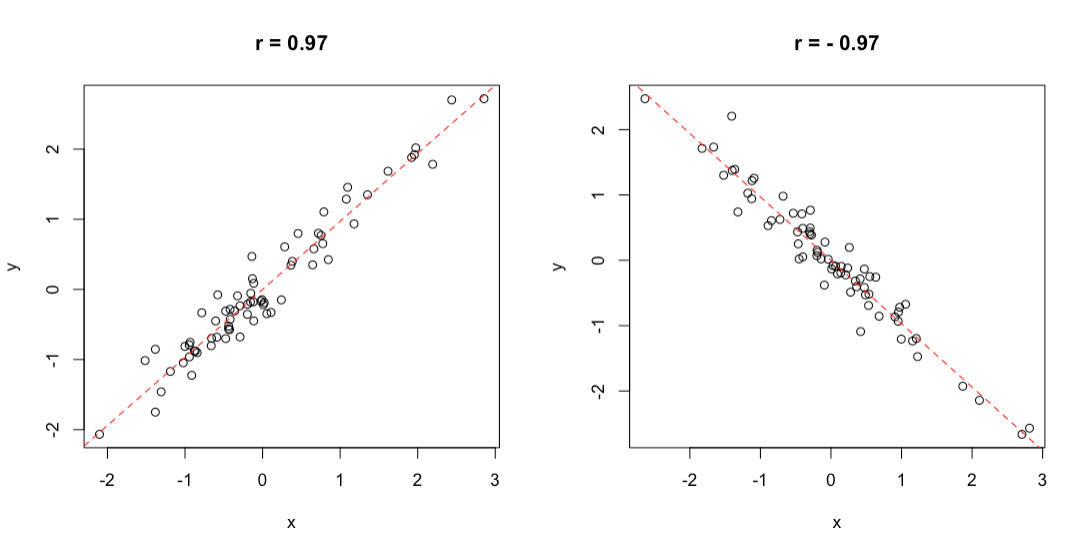
\includegraphics[width=0.85\linewidth]{_images/CorrelationExample} 

}

\caption{Esempio di correlazione positiva (destra) e negativa (sinistra)}\label{fig:figName311}
\end{figure}

Proviamo a considerare questo esempio: il contenuto di olio di 9 lotti di acheni di girasole è stato misurato con due metodi diversi ed è riportato più sotto.

\begin{Shaded}
\begin{Highlighting}[]
\NormalTok{A }\OtherTok{\textless{}{-}} \FunctionTok{c}\NormalTok{(}\DecValTok{45}\NormalTok{, }\DecValTok{47}\NormalTok{, }\DecValTok{49}\NormalTok{, }\DecValTok{51}\NormalTok{, }\DecValTok{44}\NormalTok{, }\DecValTok{37}\NormalTok{, }\DecValTok{48}\NormalTok{, }\DecValTok{44}\NormalTok{, }\DecValTok{53}\NormalTok{)}
\NormalTok{B }\OtherTok{\textless{}{-}} \FunctionTok{c}\NormalTok{(}\DecValTok{44}\NormalTok{, }\DecValTok{44}\NormalTok{, }\DecValTok{49}\NormalTok{, }\DecValTok{53}\NormalTok{, }\DecValTok{48}\NormalTok{, }\DecValTok{34}\NormalTok{, }\DecValTok{47}\NormalTok{, }\DecValTok{46}\NormalTok{, }\DecValTok{51}\NormalTok{)}
\end{Highlighting}
\end{Shaded}

Per valutare la entità della correlazione tra i risultati dei due metodi di analisi, dobbiamo eseguire alcune operazioni preliminari, cioè:

\begin{enumerate}
\def\labelenumi{\arabic{enumi}.}
\tightlist
\item
  calcolare i residui per A (\(z_A\))
\item
  calcolare i residui per B (\(z_B\))
\item
  calcolare devianze e codevianze
\end{enumerate}

In primo luogo, calcoliamo le due medie, che sono, rispettivamente, 46.44 e 46.22. Successivamente, possiamo calcolare i residui, come differenze tra ogni dato e la sua media, i loro quadrati ed i loro prodotti, come indicato in Tabella \ref{tab:tabName3}.

\begin{table}

\caption{\label{tab:tabName3}Calcolo manuale del coefficiente di correlazione}
\centering
\begin{tabular}[t]{rrrrrrr}
\toprule
A & B & \$z\_A\$ & \$z\_B\$ & \$z\_A \textbackslash{}times z\_B\$ & \$z\_A\textasciicircum{}2\$ & \$z\_B\textasciicircum{}2\$\\
\midrule
45 & 44 & -1.444 & -2.222 & 3.210 & 2.086 & 4.938\\
47 & 44 & 0.556 & -2.222 & -1.235 & 0.309 & 4.938\\
49 & 49 & 2.556 & 2.778 & 7.099 & 6.531 & 7.716\\
51 & 53 & 4.556 & 6.778 & 30.877 & 20.753 & 45.938\\
44 & 48 & -2.444 & 1.778 & -4.346 & 5.975 & 3.160\\
\addlinespace
37 & 34 & -9.444 & -12.222 & 115.432 & 89.198 & 149.383\\
48 & 47 & 1.556 & 0.778 & 1.210 & 2.420 & 0.605\\
44 & 46 & -2.444 & -0.222 & 0.543 & 5.975 & 0.049\\
53 & 51 & 6.556 & 4.778 & 31.321 & 42.975 & 22.827\\
\bottomrule
\end{tabular}
\end{table}

La somma dei quadrati dei residui ci permette di calcolare le devianze di \(A\) e \(B\) (rispettivamente 176.22 e 239.56), mentre la somme dei prodotti degli residui ci permette di calcolare la codevianza (pari a 184.11).

Il coefficiente di correlazione è quindi:

\[r = \frac{184.11}{\sqrt{176.22 \times 239.56}} = 0.896\]

Vediamo che il coefficiente di correlazione è abbastanza vicino ad 1 e quindi possiamo concludere che i due metodi di analisi danno risultati ben concordanti.

\hypertarget{statistiche-descrittive-con-r}{%
\section{Statistiche descrittive con R}\label{statistiche-descrittive-con-r}}

Le statistiche descrittive si calcolano facilmente con R. Per esercizio, utilizziamo il dataset `heights.csv', che è disponibile in una repository online. Il box sottostante mostra come caricare il dataset, del quale utilizzeremo la colonna `height' che riporta le altezze di venti piante di mais.

\begin{Shaded}
\begin{Highlighting}[]
\NormalTok{filePath }\OtherTok{\textless{}{-}} \StringTok{"https://www.casaonofri.it/\_datasets/heights.csv"}
\NormalTok{dataset }\OtherTok{\textless{}{-}} \FunctionTok{read.csv}\NormalTok{(filePath, }\AttributeTok{header =}\NormalTok{ T)}
\NormalTok{dataset}\SpecialCharTok{$}\NormalTok{height}
\DocumentationTok{\#\#  [1] 172 154 150 188 162 145 157 178 175 158 153 191 174 141 165 163}
\DocumentationTok{\#\# [17] 148 152 169 185}
\end{Highlighting}
\end{Shaded}

La media si calcola con la funzione \texttt{mean()}, mentre la mediana si calcola con la funzione \texttt{median()}.

\begin{Shaded}
\begin{Highlighting}[]
\FunctionTok{mean}\NormalTok{(dataset}\SpecialCharTok{$}\NormalTok{height)}
\DocumentationTok{\#\# [1] 164}
\FunctionTok{median}\NormalTok{(dataset}\SpecialCharTok{$}\NormalTok{height)}
\DocumentationTok{\#\# [1] 162.5}
\end{Highlighting}
\end{Shaded}

Per la devianza, non esiste una funzione dedicata e dobbiamo utilizzare l'equazione fornita in precedenza:

\begin{Shaded}
\begin{Highlighting}[]
\FunctionTok{sum}\NormalTok{( (dataset}\SpecialCharTok{$}\NormalTok{height }\SpecialCharTok{{-}} \FunctionTok{mean}\NormalTok{(dataset}\SpecialCharTok{$}\NormalTok{height))}\SpecialCharTok{\^{}}\DecValTok{2}\NormalTok{ )}
\DocumentationTok{\#\# [1] 4050}
\end{Highlighting}
\end{Shaded}

Varianza e deviazione standard sono molto facili da calcolare, grazie alle funzioni apposite, mentre il coefficiente di variabilità si può calcolare con la formula fornita in precedenza:

\begin{Shaded}
\begin{Highlighting}[]
\FunctionTok{var}\NormalTok{(dataset}\SpecialCharTok{$}\NormalTok{height)}
\DocumentationTok{\#\# [1] 213.1579}
\FunctionTok{sd}\NormalTok{(dataset}\SpecialCharTok{$}\NormalTok{height)}
\DocumentationTok{\#\# [1] 14.59993}
\FunctionTok{sd}\NormalTok{(dataset}\SpecialCharTok{$}\NormalTok{height)}\SpecialCharTok{/}\FunctionTok{mean}\NormalTok{(dataset}\SpecialCharTok{$}\NormalTok{height) }\SpecialCharTok{*} \DecValTok{100}
\DocumentationTok{\#\# [1] 8.902395}
\end{Highlighting}
\end{Shaded}

Per calcolare i percentili si usa la funzione \texttt{quantile()}, fornendo le proporzioni di soggetti da lasciare sulla sinistra con l'argomento `probs'. Ad esempio, per il 25-esimo percentile utilizzeremo 0.25, mentre per il 75-esimo utilizzeremo 0.75:

\begin{Shaded}
\begin{Highlighting}[]
\FunctionTok{quantile}\NormalTok{(dataset}\SpecialCharTok{$}\NormalTok{height, }\AttributeTok{probs =} \FunctionTok{c}\NormalTok{(}\FloatTok{0.25}\NormalTok{, }\FloatTok{0.75}\NormalTok{))}
\DocumentationTok{\#\#    25\%    75\% }
\DocumentationTok{\#\# 152.75 174.25}
\end{Highlighting}
\end{Shaded}

La correlazione si calcola invece con la funzione \texttt{cor()}, come indicato più sotto.

\begin{Shaded}
\begin{Highlighting}[]
\FunctionTok{cor}\NormalTok{(A, B)}
\DocumentationTok{\#\# [1] 0.8960795}
\end{Highlighting}
\end{Shaded}

\hypertarget{descrizione-dei-sottogruppi}{%
\subsection{Descrizione dei sottogruppi}\label{descrizione-dei-sottogruppi}}

In biometria è molto comune che il gruppo di soggetti sia divisibile in più sottogruppi, corrispondenti, ad esempio, ai diversi trattamenti sperimentali. In questa comune situazione siamo soliti calcolare, per ogni gruppo, le statistiche descrittive già viste in precedenza, utilizzando la funzione \texttt{tapply()} in R, come mostrata più sotto.

\begin{Shaded}
\begin{Highlighting}[]
\NormalTok{m }\OtherTok{\textless{}{-}} \FunctionTok{tapply}\NormalTok{(dataset}\SpecialCharTok{$}\NormalTok{height, dataset}\SpecialCharTok{$}\NormalTok{var, mean)}
\NormalTok{s }\OtherTok{\textless{}{-}} \FunctionTok{tapply}\NormalTok{(dataset}\SpecialCharTok{$}\NormalTok{height, dataset}\SpecialCharTok{$}\NormalTok{var, sd)}
\NormalTok{descript }\OtherTok{\textless{}{-}} \FunctionTok{data.frame}\NormalTok{(}\AttributeTok{Media =}\NormalTok{ m, }\AttributeTok{SD =}\NormalTok{ s)}
\NormalTok{descript}
\DocumentationTok{\#\#    Media       SD}
\DocumentationTok{\#\# C 165.00 14.36431}
\DocumentationTok{\#\# N 164.00 16.19877}
\DocumentationTok{\#\# S 160.00 12.16553}
\DocumentationTok{\#\# V 165.25 19.51709}
\end{Highlighting}
\end{Shaded}

Nel codice immediatamente precedente, \texttt{height} è la variabile che contiene i valori da mediare, \texttt{var} è la variabile che contiene la codifica di gruppo, \texttt{mean} è la funzione che dobbiamo calcolare. Ovviamente \texttt{mean} può essere sostituito da qualunque altra funzione ammissibile in R, come ad esempio la deviazione standard. Nel codice precedente abbiamo utilizzato la funzione \texttt{data.frame()} per creare una tabella riassuntiva con le medie e le deviazioni standard dei quattro gruppi.

Oltre che in una tabella, i risultati possono anche essere riportati in un grafico a barre, con l'indicazione della variabilità dei dati. Possiamo utilizzare la funzione \texttt{barplot()} alla quale passeremo come argomenti l'altezza delle barre, data dalle medie dei diversi gruppi, i nomi dei gruppi medesimi e, opzionalmente, la scala dell'asse delle ordinate. La funzione \texttt{barplot()}, oltre che creare il grafico, restituisce le ascisse del centro di ogni barra, che possiamo utilizzare per creare dei segmenti verticali corrispondenti alle deviazioni standard di ogni gruppo, attraverso la funzione \texttt{arrows()}.

L'uso di quest'ultima funzione non è immediato; poniamo che le ascisse del centro di ogni barra siano contenute nel vettore `coord'; allora i segmenti di variabilità dovranno avere punti di partenza con ascisse contenute in `coord' ed ordinate uguali all'altezza di ogni barra meno la deviazione standard. I punti di arrivo, invece, dovranno avere le stesse ascisse dei punti di partenza ed ordinate uguali all'altezza di ogni barra più la deviazione standard. Gli altri argomenti della funzione \texttt{arrows()} servono per meglio specificare l'aspetto dei segmenti di variabilità; ad esempio, il codice sottostante produce il risultato mostrato in Figura \ref{fig:figName242}; il grafico non è bellissimo, ma, con un po' di esercizio, è possibile ottenere grafici altamente professionali.

\begin{Shaded}
\begin{Highlighting}[]
\NormalTok{coord }\OtherTok{\textless{}{-}} \FunctionTok{barplot}\NormalTok{(descript}\SpecialCharTok{$}\NormalTok{Media, }\AttributeTok{names.arg =} \FunctionTok{row.names}\NormalTok{(descript), }
                 \AttributeTok{ylim =} \FunctionTok{c}\NormalTok{(}\DecValTok{0}\NormalTok{, }\DecValTok{200}\NormalTok{))}
\FunctionTok{arrows}\NormalTok{(coord, descript}\SpecialCharTok{$}\NormalTok{Media }\SpecialCharTok{{-}}\NormalTok{ descript}\SpecialCharTok{$}\NormalTok{SD, }
\NormalTok{       coord, descript}\SpecialCharTok{$}\NormalTok{Media }\SpecialCharTok{+}\NormalTok{ descript}\SpecialCharTok{$}\NormalTok{SD, }
       \AttributeTok{length =} \FloatTok{0.05}\NormalTok{, }\AttributeTok{angle =} \DecValTok{90}\NormalTok{, }\AttributeTok{code =} \DecValTok{3}\NormalTok{)}
\end{Highlighting}
\end{Shaded}

\begin{figure}

{\centering 
\includegraphics[width=0.9\linewidth]{_main_files/figure-latex/figName242-1} 

}

\caption{Esempio di boxplot in R}\label{fig:figName242}
\end{figure}

Quando abbiamo a che fare con gruppi molto numerosi, con un certo numero di outliers, è bene sostituire la mediana alla media, in associazione con il 25-esimo e 75-esimo percentile, come indicazioni di variabilità. Da un punto di vista grafico, possiamo utilizzare un \emph{boxplot} (grafico Box-Whisker). Si tratta di una scatola (box) che ha per estremi il 25-esimo e il 75-esimo percentile ed è tagliata da una linea centrale in corrispondenza della mediana. Dalla scatola partono due linee verticali (baffi = whiskers) che identificano il valore massimo e il minimo. Se il massimo (o il minimo) distano dalla mediana più di 1.5 volte la differenza tra la mediana stessa e il 75-esimo (o 25-esimo) percentile, allora le linee verticali si fermano ad un valore pari ad 1.5 volte il 75-esimo (o il 25-esimo) percentile ed i dati più estremi vengono considerati outliers e rappresentati con un piccolo cerchio. In Figura \ref{fig:figName241} abbiamo raprresentato tre gruppi di valori estratti casualmente nell'intervallo da 0 ad 1.

\begin{Shaded}
\begin{Highlighting}[]
\FunctionTok{set.seed}\NormalTok{(}\DecValTok{1234}\NormalTok{)}
\NormalTok{A }\OtherTok{\textless{}{-}} \FunctionTok{runif}\NormalTok{(}\DecValTok{20}\NormalTok{)}
\NormalTok{B }\OtherTok{\textless{}{-}} \FunctionTok{runif}\NormalTok{(}\DecValTok{20}\NormalTok{)}
\NormalTok{C }\OtherTok{\textless{}{-}} \FunctionTok{runif}\NormalTok{(}\DecValTok{20}\NormalTok{)}
\NormalTok{series }\OtherTok{\textless{}{-}} \FunctionTok{rep}\NormalTok{(}\FunctionTok{c}\NormalTok{(}\StringTok{"A"}\NormalTok{, }\StringTok{"B"}\NormalTok{, }\StringTok{"C"}\NormalTok{), }\AttributeTok{each =} \DecValTok{20}\NormalTok{)}
\NormalTok{values }\OtherTok{\textless{}{-}} \FunctionTok{c}\NormalTok{(A, B, C)}
\FunctionTok{boxplot}\NormalTok{(values }\SpecialCharTok{\textasciitilde{}}\NormalTok{ series)}
\end{Highlighting}
\end{Shaded}

\begin{figure}

{\centering 
\includegraphics[width=0.9\linewidth]{_main_files/figure-latex/figName241-1} 

}

\caption{Esempio di boxplot in R}\label{fig:figName241}
\end{figure}

\begin{center}\rule{0.5\linewidth}{0.5pt}\end{center}

\hypertarget{altre-letture-2}{%
\section{Altre letture}\label{altre-letture-2}}

\begin{enumerate}
\def\labelenumi{\arabic{enumi}.}
\tightlist
\item
  F. Crivellari (2006). Analisi statistica dei dati con R. Apogeo, Milano.
\item
  G. Leti and L. Cerbara (2009). Elementi di statistica descrittiva. Il Mulino Editore, Bologna.
\item
  R.R Sokal and Rohlf, F.J. (1981). Biometry. W.H. Freeman and Company, Books.
\end{enumerate}

\hypertarget{domande-ed-esercizi-1}{%
\section{Domande ed esercizi}\label{domande-ed-esercizi-1}}

\begin{enumerate}
\def\labelenumi{\arabic{enumi}.}
\tightlist
\item
  Illustrare e discutere i principali indici di tendenza centrale per le variabili quantitative
\item
  Illustrare e discutere i principali indici di variabilità per le variabili quantitative
\item
  Illustrare e discutere il coefficiente di correlazione di Pearson
\item
  Un'analisi chimica è stata eseguita in triplicato e i risultati sono stati i seguenti: 125, 169 and 142 ng/g. Calcolate la media e tutti gli indicatori di variabilità che conoscete. In che modo può essere espressa l'incertezza assoluta della misura?
\item
  Un ricercatore ha misurato l'altezza di quattro alberi ed il loro diametro (entrambi in metri). I risultati ottenuti sono i seguenti: \texttt{Altezza\ \textless{}-\ c(2.3,\ 2.7,\ 3.1,\ 3.5)} e \texttt{Diametro\ \textless{}-\ c(0.46,\ 0.51,\ 0.59,\ 0.64)}. Calcolare il coefficiente di correlazione di Pearson e valutare l'entità della correlazione in base ai valori massimi e minimi ammissibili per questa statistica.
\item
  Considerate il file EXCEL `rimsulfuron.csv', che potete trovare in questo percorso: \url{https://www.casaonofri.it/_datasets/rimsulfuron.csv}. In questo file sono riportati i risultati di un esperimento con 16 trattamenti e 4 repliche, nel quale sono stati posti a confronti diversi erbicidi e/o dosi per il diserbo nel mais. Calcolare le medie produttive ottenute con le diverse tesi sperimentali e riportarle su un grafico, includendo anche un'indicazione di variabilità. Verificare se la produzione è correlata con il ricoprimento (WeedCover) delle piante infestanti.
\end{enumerate}

\hypertarget{le-relazioni-causa-effetto}{%
\chapter{Le relazioni causa-effetto}\label{le-relazioni-causa-effetto}}

Nel capitolo precedente abbiamo visto come possiamo utilizzare semplici statistiche per descrivere alcuni tratti dei nostri dati sperimentali, come la tendenza centrale e la dispersione e, se abbiamo due o più variabili, abbiamo visto come possiamo descrivere la loro variabilità congiunta, utilizzando il coefficiente di correlazione.

Nel lavoro di ricerca, la relazione tra variabili più importante è la cosiddetta \textbf{causalità}, che si verifica ogni volta che una variabile (solitamente denominata ``predittore'') provoca un cambiamento in un'altra variabile (solitamente denominata ``risposta''); ad esempio, una variazione del genotipo può causare un cambiamento nella resa del frumento, oppure una variazione nella tecnica di lavorazione può causare un cambiamento nel tempo di emergenza del mais. Questo effetto diretto del predittore sulla risposta (e non viceversa) è ciò che rende la causalità diversa, ad esempio, dalla correlazione, che implica solo variazione congiunta, senza una chiara distinzione tra predittore e risposta, cioè tra la causa e l'effetto.

Gli esperimenti controllati, replicati e randomizzati sono particolarmente adatti a stabilire relazioni causa-effetto; infatti, la probabilità di effetti confondenti è ridotta al minimo, così che le discrepanze tra le unità osservate sottoposte a trattamenti diversi possono essere ragionevolmente attribuite all'effetto di tali trattamenti sperimentali e non ad altre cause sistematiche, ma ignote.

\hypertarget{modelli-matematici-e-statistici}{%
\section{Modelli matematici e statistici}\label{modelli-matematici-e-statistici}}

Per descrivere le relazioni causali, possiamo utilizzare i \textbf{modelli statistici}, cioè delle equazioni in cui le osservazioni sperimentali sono prodotte come risultato dell'effetto di uno o più predittori.

Si può ritenere che l'impiego di modelli matematici per la descrizione dei fenomeni scientifici sia iniziato con Galilei e si poi sviluppato negli anni seguenti, fino a portare all'ambizione più grande degli scienziati all'inizio dell'ottocento, che era quella di poter prevedere l'evoluzione di un sistema scientifico, semplicemente conoscendone lo stato iniziale e l'insieme di tutte le forze che agivano su di esso. Ad esempio, Laplace diceva: \emph{``Possiamo considerare lo stato attuale dell'universo come l'effetto del suo passato e la causa del suo futuro. Un intelletto che ad un determinato istante dovesse conoscere tutte le forze che mettono in moto la natura, e tutte le posizioni di tutti gli oggetti di cui la natura è composta, se questo intelletto fosse inoltre sufficientemente ampio da sottoporre questi dati ad analisi, esso racchiuderebbe in un'unica formula i movimenti dei corpi più grandi dell'universo e quelli degli atomi più piccoli; per un tale intelletto nulla sarebbe incerto ed il futuro proprio come il passato sarebbe evidente davanti ai suoi occhi''}. In realtà si è ben presto scoperto che si trattava di un'ambizione irrealistica, non tanto e non solo per la comparsa della meccanica quantistica un secolo dopo, ma anche per l'aumento di importanza degli studi in ambito psichiatrico e medico/biologico. Questi studi, infatti, venivano (e vengono) eseguiti su organismi viventi molto complessi, che, se sottoposti allo stesso stimolo, davano (e danno) risposte altamente variabili e, spesso, anche difficilmente misurabili e controllabili.

Queste difficoltà fecero prevalere, tra i biologi, la convinzione che la natura funzionasse in base a meccanismi deterministici ben definiti, anche se difficilmente osservabili nella pratica sperimentale, a causa dei numerosi elementi d'incertezza che si manifestavano nel corso delle osservazioni sperimentali. Insomma, la natura è perfetta, ma l'osservazione è fallace, perché influenzata dalla presenza di una forte componente stocastica ed imprevedibile, che va sotto il nome generico di errore sperimentale. Di questo abbiamo già parlato nei capitoli precedenti. Abbiamo anche visto che Ronald Fisher, nel suo famoso testo ``Il disegno degli esperimenti'' ha posto le basi per una corretta metodica sperimentale, finalizzata a minimizzare l'impatto della componente stocastica e, soprattutto, ad impedire che essa si confondesse con gli effetti degli stimoli sperimentali in studio.

Minimizzare, tuttavia, non significa eliminare ed è evidente che, pur con tutti gli sforzi possibili, è impossibile evitare che i risultati sperimentali siano influenzati, sempre e comunque, da una certa quota di variabilità stocastica. Si vengono quindi a creare due contrapposte situazioni:

\begin{enumerate}
\def\labelenumi{\arabic{enumi}.}
\tightlist
\item
  la verità `vera', immanente, che `agisce' in base a meccanismi deterministici causa-effetto ben definiti.
\item
  La `verità' sperimentale, che si produce a partire dalla verità `vera', per effetto dell'azione di elementi perturbativi casuali, che non ci permettono di osservare la verità `vera'.
\end{enumerate}

Di conseguenza, la descrizione di qualunque risultato sperimentale non può essere realistica se non utilizzando un modello in grado di considerare contemporaneamente sia i nessi causa-effetto, che le altre forze ignote e, almeno apparentemente, di natura stocastica. Come abbiamo anticipato più sopra, i modelli matematici che incorporano anche effetti di natura casuale sono detti modelli statistici.

\hypertarget{componenti-di-un-modello}{%
\section{Componenti di un modello}\label{componenti-di-un-modello}}

In semplice linguaggio algebrico, possiamo scrivere un modello causa-effetto utilizzando un'a funzione'equazione generale come la seguente:

\[ Y_E = f(X, \theta)\]

dove \(Y_E\) è l'effetto atteso dello stimolo \(X\), secondo la funzione \(f\), basata su una collezioni di parametri \(\theta\)

Le componenti di questo modello sono la risposta attesa (\(Y_E\)) che è l'oggetto del nostro studio e può assumere le forme più disparate: spesso è numerica, ma a volte rappresenta una qualità. In questo libro consideremo solo la situazione in cui \(Y_E\) è rappresentato da una sola variabile (analisi univariata), ma esistono casi in cui viene osservata ed analizzata la risposta di soggetti in relazione a molte variabili (analisi multivariata).

Lo stimolo sperimentale (\(X\)) è costituito da una o più variabili continue, discrete o categoriche (predittori), che rappresentano i trattamenti sperimentali. Insieme ad \(Y_E\), \(X\) è l'elemento noto di un esperimento, in quanto viene definito \emph{a priori} in fase di progettazione.

La `funzione' di risposta (\(f\)) è un'equazione, lineare o non-lineare, scelta in base a considerazioni di carattere biologico, o con un approccio puramente empirico, osservando l'andamento della curva di risposta.

I parametri di una funzione (\(\theta\)) sono un insieme di valori numerici che permettono di definire l'equazione di risposta.

Il predittore può essere rappresentato da una dose; ad esempio un aumento della dose di una sostanza erbicida provoca una diminuzione della crescita delle erbe infestanti. In questo caso usiamo il termine \emph{modello dose-risposta}, che è forse uno dei modelli più famosi e viene fatto risalire a Paracelso (1493-1541), con il famoso aforisma: ``\emph{Cosa c'è che non sia veleno? Tutte le cose sono veleno e nulla è senza veleno. Soltanto la dose determina cosa sia un veleno}''.

Il modello sovrastante, in accordo con la logica galileiana, postula che un fenomeno naturale segua una legge ben definita. Tuttavia, la realtà è più complessa delle nostre aspettative e, a causa di errori sperimentali e altri effetti di natura puramente casuale, non osserviamo mai il risultato atteso \(Y_E\), ma osserviamo un valore diverso \(Y_O \neq Y_E\). Dobbiamo quindi ampliare il modello aggiungendo la componente stocastica \(\varepsilon\):

\[ Y_O = f(X, \theta) + \varepsilon\]

cioè il cosiddetto `residuo', la discrepanza tra ciò che prevede il modello e ciò che effettivamente osserviamo:

\[\varepsilon = Y_O - Y_E \]

In un esperimento con \(n\) unità sperimentali, abbiamo \(n\) residui, con media pari a 0 e deviazione standard pari a \(\sigma\) (in inglese si utilizza anche l'acronimo RMSE, ossia `Root Mean Squared Error'). \textbf{I residui misurano quanto ``cattivo'' è il modello: tanto più sono alti, quanto più le previsioni si discostano dalle osservazioni, inficiando la capacità del modello di descrivere una certa relazione causa-effetto}.

\hypertarget{fitting-di-un-modello}{%
\section{\texorpdfstring{\emph{Fitting} di un modello}{Fitting di un modello}}\label{fitting-di-un-modello}}

Nella ricerca, possiamo utilizzare i modelli per capire se due o più variabili sperimentali sono in una relazione causa-effetto tra di loro. Il nostro lavoro consisterà nel:

\begin{enumerate}
\def\labelenumi{\arabic{enumi}.}
\tightlist
\item
  definire un modello statistico potenzialmente capace di descrivere adeguatamente le relazioni causa-effetto in studio, traducendo in termini matematici l'ipotesi scientifica di partenza. Questo modello sarà posto nella sua forma generale e sarà basato su una serie di parametri dal valore ignoto (\(\theta\) e \(\sigma\)).
\item
  Eseguire l'esperimento e raccogliere i dati.
\item
  Utilizzare il set di dati per assegnare valori precisi a tutti i parametri ignoti (\textbf{fitting del modello} o, in alcune applicazioni, \textbf{calibrazione del modello}).
\item
  Valutare se il modello parametrizzato fornisca una descrizione accurata dei dati sperimentali (\textbf{valutazione del modello}).
\item
  Se necessario, in presenza di ipotesi scientifiche alternative tradotte in altrettanti modelli matematici, selezionare il modello migliore quelli proposti (\textbf{confronto dei modelli}).
\end{enumerate}

Il fitting del modello viene solitamente eseguito dall'algoritmo dei ``minimi quadrati'', che consiste nel selezionare i valori dei parametri che minimizzano la somma dei residui al quadrato (RSS: Residual Sum of Squares):

\[RSS = \sum_{i = 1}^n{\left( Y_{O_i} - Y_{E_i} \right)^2}\]

In generale, la minimizzazione dei quadrati dei residui non viene eseguita mediante calcoli manuali, in quanto è molto più semplice avvalersi delle funzioni di adattamento più adatte in R. In particolare, per i modelli lineari utilizzeremo la funzione \texttt{lm()}, con la seguente sintassi:

\begin{verbatim}
mod <- lm(Y ~ X dati = set di dati)
\end{verbatim}

Il primo argomento è l'equazione che vogliamo adattare: sul lato sinistro dobbiamo specificare il nome della variabile di risposta, la `tilde' (\textasciitilde) significa `è una funzione di' e sostituisce il segno `=', mentre, sul lato destro, dobbiamo specificare il nome del/i predittore/i. Come secondo argomento, se necessario, forniamo il nome del dataset in cui sono archiviate le variabili. Non dobbiamo specificare l'intercetta e il termine stocastico \(\varepsilon\), che sono inclusi per impostazione predefinita.

Per evitare errori, è necessario ricordare che un predittore \(X\) può essere costituito da una variabile quantitativa oppure da una variabile categorica e i due tipi di variabili identificano tipologie di modelli molto diversi tra di loro. Può capitare di avere a che fare con un predittore qualitativo per cui le classi sono espresse in formato numerico, come ad esempio i blocchi, che potrebbero essere indicati con i valori 1, 2, 3, e 4, senza che questi valori rappresentino veramente una quantità. In tutte queste situazione e, suggerirei in ogni caso, quando intendiamo procedere al fitting di un modello in cui qualcuno dei predittori è una variabile categorica, \textbf{dovremmo esplicitamente trasformarla in un vettore di tipo `factor'}, per evitare che R la interpreti erroneamente come una quantità, adattando il modello sbagliato. La trasformazione si effettua, nel modo più semplice, con il codice seguente:

\begin{verbatim}
X <- factor(X)
\end{verbatim}

Un modello completamente specificato può fornire una buona descrizione dei dati sperimentali, \textbf{postulando l'esistenza di un meccanismo causa-effetto ben definito}. Con la dovuta prudenza, questo modello può essere utilizzato per fare previsioni; ad esempio, se i dati sperimentali hanno suggerito che l'effetto della concimazione azotata sul frumento può essere rappresentata con una retta con equazione \(Y_E = b_0 + b_1 \, X\), dove \(b_0 = 65\) e \(b_1 = 0.1\), allora si potrebbe concludere che una concimazione con 150 kg/ha di azoto dovrebbe, prevedibilmente, dare come risultato un livello di resa \(Y_E = 80\) quintali per ettaro.

\hypertarget{esempio-1-il-modello-della-media}{%
\section{Esempio 1: il `modello della media'}\label{esempio-1-il-modello-della-media}}

Abbiamo condotto un esperimento misurativo, in cui abbiamo raccolto tre campioni di acqua da un pozzo, per misurare la concentrazione di una sostanza xenobiotica. I risultati sono 116, 119, 125 mg/L e vogliamo calcolare la media e la deviazione standard dei tre campioni.

Questo problema è piuttosto semplice e potrebbe essere meglio risolto utilizzando semplici statistiche descrittive (vedi Capitolo 3); tuttavia, è interessante vedere come lo stesso problema può essere posto in una logica di `model fitting': non abbiamo alcun predittore e, pertanto, possiamo supporre che le osservazioni siano generate in base al modello della media: \(Y_i = \mu + \varepsilon_i\), dove l'elemento stocastico ha media 0 e una deviazione standard \(\sigma\).

Assegnare un valore a tutti i parametri sconosciuti è banale, utilizzando i semplici calcoli mostrati nel Capitolo 3 (vale a dire, \(\mu = 120\) e \(\sigma = 4.58\)). Tuttavia, possiamo ottenere gli stessi risultati utilizzando l'approccio di minimizzazione dei minimi quadrati, come mostrato nel riquadro seguente. Si noti che utilizziamo `1' come lato destro dell'equazione del modello, poiché non abbiamo alcun predittore.

\vspace{12pt}

\begin{Shaded}
\begin{Highlighting}[]
\NormalTok{Y }\OtherTok{\textless{}{-}} \FunctionTok{c}\NormalTok{(}\DecValTok{116}\NormalTok{, }\DecValTok{119}\NormalTok{, }\DecValTok{125}\NormalTok{)}
\NormalTok{mod }\OtherTok{\textless{}{-}} \FunctionTok{lm}\NormalTok{(Y }\SpecialCharTok{\textasciitilde{}} \DecValTok{1}\NormalTok{)}
\end{Highlighting}
\end{Shaded}

La stima di \(\mu\) può essere ottenuta con la seguente funzione R:

\vspace{12pt}

\begin{Shaded}
\begin{Highlighting}[]
\FunctionTok{coef}\NormalTok{(mod)}
\DocumentationTok{\#\# (Intercept) }
\DocumentationTok{\#\#         120}
\end{Highlighting}
\end{Shaded}

Per quanto riguarda la componente stocastica, possiamo ottenere i residui, la loro devianza e la loro deviazione standard con le seguenti funzioni R:

\vspace{12pt}

\begin{Shaded}
\begin{Highlighting}[]
\CommentTok{\# Residui}
\FunctionTok{residuals}\NormalTok{(mod)}
\DocumentationTok{\#\#  1  2  3 }
\DocumentationTok{\#\# {-}4 {-}1  5}
\CommentTok{\#}
\CommentTok{\# Devianza dei residui}
\FunctionTok{deviance}\NormalTok{(mod)}
\DocumentationTok{\#\# [1] 42}
\CommentTok{\#}
\CommentTok{\# Deviazione standard dei residui}
\FunctionTok{summary}\NormalTok{(mod)}\SpecialCharTok{$}\NormalTok{sigma}
\DocumentationTok{\#\# [1] 4.582576}
\end{Highlighting}
\end{Shaded}

Il modello della media descrive una situazione in cui non abbiamo predittori e, pertanto, non vi sono nessi causa-effetto; di conseguenza, è il peggior modello possibile, il punto di riferimento rispetto al quale valutare ogni altro modello alternativo. Per queste sue caratteristiche, il modello della media è spesso definito come \textbf{modello nullo}.

\hypertarget{esempio-2-un-predittore-quantitativo}{%
\section{Esempio 2: un predittore quantitativo}\label{esempio-2-un-predittore-quantitativo}}

L'algoritmo dei minimi quadrati è facile da comprendere se consideriamo un esperimento in cui la resa del mais (la risposta, in t/ha) sia stata determinata in funzione del ricoprimento delle piante infestanti (il predittore, in \%), determinato all'inizio del ciclo colturale. In una situazione del genere, potremmo ipotizzare un modello lineare (linea retta) del tipo: \(Y_i = b_0 + b_1 \, X_i + \varepsilon_i\), che è solitamente noto come \textbf{modello di regressione lineare semplice}.

I due parametri \(b_0\) e \(b_1\) rappresentano, rispettivamente, l'intercetta (livello di resa senza infestanti) e la pendenza (variazione della resa per ogni aumento unitario del ricoprimento). Per stimare questi due valori, possiamo usare la funzione `lm()', che produce i risultati mostrati nella Figura \ref{fig:figName41a}.

\begin{Shaded}
\begin{Highlighting}[]
\CommentTok{\# Fitting a simple linear regression model}

\CommentTok{\# Entering the data}
\FunctionTok{library}\NormalTok{(statforbiology)}
\NormalTok{dataset }\OtherTok{\textless{}{-}} \FunctionTok{getAgroData}\NormalTok{(}\StringTok{"WeedCover"}\NormalTok{)}

\CommentTok{\# Fitting the model}
\NormalTok{mod }\OtherTok{\textless{}{-}} \FunctionTok{lm}\NormalTok{(Yield }\SpecialCharTok{\textasciitilde{}}\NormalTok{ WeedCover, }\AttributeTok{data =}\NormalTok{ dataset)}

\CommentTok{\# Inspecting the estimates}
\FunctionTok{coef}\NormalTok{(mod)}
\DocumentationTok{\#\# (Intercept)   WeedCover }
\DocumentationTok{\#\# 10.65979798 {-}0.06033652}
\end{Highlighting}
\end{Shaded}

\begin{figure}

\includegraphics[width=0.85\linewidth]{_main_files/figure-latex/figName41a-1} \caption{Example 2: the least square estimate is represented by the straight line that passes as close as possible to the observed points.}\label{fig:figName41a}
\end{figure}

\hypertarget{esempio-3-un-predittore-nominale}{%
\section{Esempio 3: un predittore nominale}\label{esempio-3-un-predittore-nominale}}

Immaginiamo un esperimento sul campo per confrontare la resa di quattro genotipi di avena (denominati A, B, C e D), con un disegno completamente randomizzato con tre repliche. I risultati (in tonnellate per ettaro) sono mostrati nella Tabella \ref{tab:tabName4b1}.

\begin{longtable}[]{@{}lrrr@{}}
\caption{\label{tab:tabName4b1}Esempio di una dataset proveniente da una prova varietale a randomizzazione completa con quattro genotipi di avena (A, B, C and D) e tre repliche.}\tabularnewline
\toprule()
Genotype & 1 & 2 & 3 \\
\midrule()
\endfirsthead
\toprule()
Genotype & 1 & 2 & 3 \\
\midrule()
\endhead
A & 4.50 & 4.65 & 4.59 \\
B & 3.70 & 3.38 & 3.58 \\
C & 4.17 & 3.94 & 4.14 \\
D & 4.76 & 4.48 & 4.55 \\
\bottomrule()
\end{longtable}

In questo esperimento, abbiamo una risposta quantitativa (la resa) e un fattore nominale (il genotipo) e la relazione causa-effetto tra queste due variabili può essere descritta con il modello seguente:

\[Y_i = \mu + \alpha_j + \varepsilon_i\]

Questo modello postula che ogni osservazione \(Y_i\) derivi dal valore \(\mu\) (la cosiddetta intercetta) più le quantità \(\alpha_j\), che dipendono dal genotipo \(j\), più gli effetti stocastici \(\varepsilon_i\), che sono specifici per ogni osservazione ed hanno media 0 e una deviazione standard pari a \(\sigma\).

Per comprendere il significato biologico di \(\mu\) ed \(\alpha\) dobbiamo entrare un po' di più nei dettagli matematici. Consideriamo la prima osservazione \(Y_1 = 4.5\); dobbiamo stimare tre valori (\(\mu\), \(\alpha_1\) e \(\varepsilon_1\)) che, sommati, restituiscano questa osservazione. Chiaramente il problema è indeterminato, in quanto esistono infinite triplette di valori, che, sommate, restituiscono 4.5; pertanto è necessario imporre dei vincoli su alcuni parametri del modello (\textbf{parametrizzazioni del modello}). Un vincolo molto comune è \(\alpha_1 = 0\) (\textbf{vincolo sul trattamento}):

\[\left\{ {\begin{array}{l}
\mu_1 = \mu + \alpha_1 = \mu + 0\\
\mu_2 = \mu + \alpha_2 \\
\mu_3 = \mu + \alpha_3 \\
\mu_4 = \mu + \alpha_4
\end{array}} \right.\]

Con tale vincolo, \(\mu\) è la media del primo genotipo (in R: \textbf{primo in ordine alfabetico}), mentre \(\alpha_2\), \(\alpha_3\) e \(\alpha_4\) sono, rispettivamente, le differenze tra le medie del secondo, terzo e quarto genotipo,
rispetto al primo. In generale, con questa parametrizzazione, i parametri del modello sono medie o differenze tra medie.

Un altro possibile vincolo è \(\sum{\alpha_j} = 0\) (vincolo sulla somma). Se prendiamo l'equazione precedente e sommiamo tutti i membri otteniamo:

\[\mu_1 + \mu_2 + \mu_3 + \mu_4 = 4 \mu + \sum{\alpha_j}\]

Imponendo il vincolo di somma a zero otteniamo:

\[\mu_1 + \mu_2 + \mu_3 + \mu_4 = 4 \mu\]

e quindi a:

\[\mu = \frac{\mu_1 + \mu_2 + \mu_3 + \mu_4}{4}\]

Con questa parametrizzazione \(\mu\) è la media generale dei dati, mentre i valori \(\alpha_j\) rappresentano le differenze tra le medie dei trattamenti e la media generale (\textbf{effetti dei trattamenti}): valori \(\alpha\) positivi ed elevati identificano i genotipi superiori alla media, mentre valori \(\alpha\) elevati, ma negativi identificano i genotipi inferiori alla media. In generale, con questa parametrizzazione, i parametri del modello rappresentano medie ed effetti.

Un terzo possibile vincolo si ottiene rimuovendo l'intercetta (ovvero, imponendo che \(\mu = 0\)). In questo caso, i valori di \(\alpha_j\) saranno le medie dei genotipi ed il modello riduce a:

\[Y_i = \mu_j + \varepsilon_i\]

La selezione dei vincoli spetta all'utente, a seconda degli obiettivi dell'esperimento. \textbf{In R, il vincolo del trattamento è utilizzato di default}, sebbene gli altri vincoli possano essere facilmente ottenuti, utilizzando la codifica appropriata.

La stima dei parametri del modello potrebbe essere facilmente eseguita a mano, ma noi utilizziamo la funzione `lm()' in R.

\vspace{12pt}

\begin{Shaded}
\begin{Highlighting}[]
\NormalTok{mod }\OtherTok{\textless{}{-}} \FunctionTok{lm}\NormalTok{(Yield }\SpecialCharTok{\textasciitilde{}}\NormalTok{ Genotype, }\AttributeTok{data =}\NormalTok{ dataset)}
\end{Highlighting}
\end{Shaded}

I parametri stimati, i residui, la deviazione residua e la deviazione standard possono essere ottenuti con la solita codifica:

\vspace{12pt}

\begin{Shaded}
\begin{Highlighting}[]
\CommentTok{\# Stima dei parametri}
\FunctionTok{coef}\NormalTok{(mod)}
\DocumentationTok{\#\# (Intercept)   GenotypeB   GenotypeC   GenotypeD }
\DocumentationTok{\#\#  4.58000000 {-}1.02666667 {-}0.49666667  0.01666667}
\CommentTok{\#}
\CommentTok{\# Residui}
\FunctionTok{residuals}\NormalTok{(mod)}
\DocumentationTok{\#\#           1           2           3           4           5 }
\DocumentationTok{\#\# {-}0.08000000  0.07000000  0.01000000  0.14666667 {-}0.17333333 }
\DocumentationTok{\#\#           6           7           8           9          10 }
\DocumentationTok{\#\#  0.02666667  0.08666667 {-}0.14333333  0.05666667  0.16333333 }
\DocumentationTok{\#\#          11          12 }
\DocumentationTok{\#\# {-}0.11666667 {-}0.04666667}
\CommentTok{\#}
\CommentTok{\# Devianza dei residui}
\FunctionTok{deviance}\NormalTok{(mod)}
\DocumentationTok{\#\# [1] 0.1374}
\CommentTok{\#}
\CommentTok{\# Deviazione standard del residui (RMSE)}
\FunctionTok{summary}\NormalTok{(mod)}\SpecialCharTok{$}\NormalTok{sigma}
\DocumentationTok{\#\# [1] 0.1310534}
\end{Highlighting}
\end{Shaded}

Ora che il modello è completamente specificato, abbiamo tutti gli ingredienti per descrivere le 12 osservazioni, sommando \(\mu + \alpha_j + \varepsilon_i\); ad esempio, per la prima osservazione, appartenente al primo genotipo, abbiamo:

\[y_1 = 4.5 = 4.533 + 0 - 0.033\]
mentre, per la quarta osservazione, appartenente al 2° genotipo, abbiamo:

\[y_4 = 3.9 = 4.533 - 0.7 + 0.067\]

Per completezza, potrebbe essere utile mostrare che, in R, possiamo modificare la parametrizzazione, impostando l'argomento `contrasts' e passando un elenco di fattori associati alla parametrizzazione richiesta. Ad esempio, se utilizziamo \texttt{Treat\ =\ "contr.sum"}, otteniamo il vincolo sulla somma; di conseguenza, l'effetto dell'ultimo genotipo non è mostrato, perché è vincolato ad eseere l'opposto della somma degli altri tre effetti.

\vspace{12pt}

\begin{Shaded}
\begin{Highlighting}[]
\NormalTok{mod2 }\OtherTok{\textless{}{-}} \FunctionTok{lm}\NormalTok{(Yield }\SpecialCharTok{\textasciitilde{}}\NormalTok{ Genotype,}
           \AttributeTok{contrasts =} \FunctionTok{list}\NormalTok{(}\AttributeTok{Genotype =} \StringTok{"contr.sum"}\NormalTok{),}
           \AttributeTok{data =}\NormalTok{ dataset)}
\FunctionTok{coef}\NormalTok{(mod2)}
\DocumentationTok{\#\# (Intercept)   Genotype1   Genotype2   Genotype3 }
\DocumentationTok{\#\#   4.2033333   0.3766667  {-}0.6500000  {-}0.1200000}
\end{Highlighting}
\end{Shaded}

Un'altra possibile parametrizzazione consiste nel rimuovere l'intercetta, che è possibile utilizzando \texttt{-1} sul lato destro dell'espressione, come mostrato di seguito.

\vspace{12pt}

\begin{Shaded}
\begin{Highlighting}[]
\NormalTok{mod3 }\OtherTok{\textless{}{-}} \FunctionTok{lm}\NormalTok{(Yield }\SpecialCharTok{\textasciitilde{}}\NormalTok{ Genotype }\SpecialCharTok{{-}} \DecValTok{1}\NormalTok{, }\AttributeTok{data =}\NormalTok{ dataset)}
\FunctionTok{coef}\NormalTok{(mod3)}
\DocumentationTok{\#\# GenotypeA GenotypeB GenotypeC GenotypeD }
\DocumentationTok{\#\#  4.580000  3.553333  4.083333  4.596667}
\end{Highlighting}
\end{Shaded}

Esistono diversi altri metodi per modificare la parametrizzazione, sia globalmente (per l'intera sessione R) sia a livello di fattore; ulteriori informazioni sono disponibili in letteratura.

\hypertarget{lanalisi-della-varianza-anova}{%
\section{L'analisi della varianza (ANOVA)}\label{lanalisi-della-varianza-anova}}

In questo secondo esempio abbiamo descritto una relazione causa-effetto, tramite un modello contenente un predittore. L'RMSE (\(\sigma\)) è uguale a 0.131, ma questa non è una buona metrica per capire se la relazione causa-effetto è rilevante o meno. Una possibilità è quella di dividere l'RMSE per la media dei valori osservati, per ottenere il coefficiente di variabilità (RRMSE: Relative Root Mean Squared Error), che è 0.031 (o 3.1\%), il che indica che l'errore residuo è piuttosto piccolo, rispetto al valore medio atteso.

Un altro indicatore per descrivere la bontà della relazione causa-effetto definita dal modello è il cosiddetto \textbf{coefficiente di determinazione (R\textsuperscript{2})}, ottenuto sottraendo da 1 il rapporto tra la devianza dei residui e la devianza totale delle osservazioni (che poi sarebbe la devianza dei residui del modello nullo). Nel nostro caso, il modello nullo è ottenuto trascurando l'effetto del genotipo e la devianza dei residui è quella indicata nel box sottostante:

\begin{Shaded}
\begin{Highlighting}[]
\NormalTok{modnull }\OtherTok{\textless{}{-}} \FunctionTok{lm}\NormalTok{(Yield }\SpecialCharTok{\textasciitilde{}} \DecValTok{1}\NormalTok{, }\AttributeTok{data =}\NormalTok{ dataset)}
\FunctionTok{deviance}\NormalTok{(modnull)}
\DocumentationTok{\#\# [1] 2.337867}
\end{Highlighting}
\end{Shaded}

Il coefficiente di determinazione è quindi:

\[R^2 = 1 - \frac{SS_{res}}{SS_{tot}} = 1 - \frac{0.1374}{2.337867} = 0.94123\]

cosa che può essere verificata utilizzando il codice R:

\begin{Shaded}
\begin{Highlighting}[]
\FunctionTok{summary}\NormalTok{(mod)}\SpecialCharTok{$}\NormalTok{r.squared}
\DocumentationTok{\#\# [1] 0.9412285}
\end{Highlighting}
\end{Shaded}

Il coefficiente di determinazione varia da 0 ad 1, più è alto il valore tanto migliore è la bontà del modello.

Oltre a queste statistiche (RMSE, RRMSE e R\textsuperscript{2}), vi è una tecnica famosissima per valutare l'entità dell'evidenza in favore dell'esistenza di una relazione causa effetto ben definita; questa tecnica si chiama \textbf{Analisi della Varianza (ANOVA)} ed è stata originariamente ideata da Ronald Fisher durante gli anni '30 del XX secolo; oggi è ancora molto utilizzata, seppure in una forma leggermente diversa da quella originale.

Il principio di fondo è che, considerando un modello che contenga almeno un predittore, è sempre possibile associare allo stesso dataset un secondo modello `nullo' (modello della media), ottenuto dal precedente per rimozione del predittore. Ad esempio, con riferimento all'esempio 2, abbiamo già visto che il modello ANOVA è:

\begin{verbatim}
Yield ~ Genotype
\end{verbatim}

mentre il modello nullo è:

\begin{verbatim}
Yield ~ 1
\end{verbatim}

Rimuovere l'effetto del genotipo dal modello non può che indurre un incremento dei residui, dato che non si tiene più in considerazione il fatto che parte della differenza tra le osservazioni è dovuto al fatto che esse appartengono a genotipi diversi. Infatti, il codice sovrastante e sottostante mostrano che la devianza dei residui (RSS: Residual Sum of Squares) è pari a:

\begin{Shaded}
\begin{Highlighting}[]
\NormalTok{epsilon }\OtherTok{\textless{}{-}} \FunctionTok{residuals}\NormalTok{(mod)}
\NormalTok{RSS }\OtherTok{\textless{}{-}} \FunctionTok{sum}\NormalTok{(epsilon}\SpecialCharTok{\^{}}\DecValTok{2}\NormalTok{)}
\NormalTok{RSS}
\DocumentationTok{\#\# [1] 0.1374}
\end{Highlighting}
\end{Shaded}

mentre la devianza dei residui del modello nullo (pari alla devianza totale delle osservazioni), è pari a:

\begin{Shaded}
\begin{Highlighting}[]
\CommentTok{\# Residual deviance null model}
\NormalTok{RSS.null }\OtherTok{\textless{}{-}} \FunctionTok{sum}\NormalTok{(}\FunctionTok{residuals}\NormalTok{(modnull)}\SpecialCharTok{\^{}}\DecValTok{2}\NormalTok{)}
\NormalTok{RSS.null}
\DocumentationTok{\#\# [1] 2.337867}
\end{Highlighting}
\end{Shaded}

Insomma, rimuovendo l'effetto del genotipo, il modello è `peggiorato', con un incremento dei residui quantificabile come differenza:

\begin{Shaded}
\begin{Highlighting}[]
\CommentTok{\# Contribution of genotype effect}
\NormalTok{SS\_g }\OtherTok{\textless{}{-}}\NormalTok{ RSS.null }\SpecialCharTok{{-}}\NormalTok{ RSS}
\NormalTok{SS\_g}
\DocumentationTok{\#\# [1] 2.200467}
\end{Highlighting}
\end{Shaded}

È evidente che più è grande questa differenza, più è grande l'effetto del genotipo. In altre parole, abbiamo appena scomposto la devianza totale delle osservazioni (\(SS_{tot} = 2.337867\)) in due quote, una dovuta all'effetto causale del trattamento sperimentale (\(SS_g = 2.200\)) e l'altra dovuta a tutti gli altri effetti ignoti di natura casuale (errore sperimentale: \(RSS = 2.337867\)). Questa seconda quota costituisce una specie di `rumore di fondo', contro il quale si può valutare il `segnale', cioè l'intensità dell'effetto del trattamento sperimentale.

Come abbiamo visto nel Capitolo 3, non possiamo confrontare direttamente \(SS_g\) e \(RSS\), poiché queste due devianze hanno un diverso numero di gradi di libertà (DF); il numero di DF per il trattamento è uguale al numero dei suoi livelli meno uno (\(DF_g\) = 3), mentre il numero di gradi di libertà per la devianza residua \(RSS\) è \(p \times (k -1)\), dove \(p\) è il numero di trattamenti e \(k\) è il numero di repliche, supponendo che questo sia costante tra i trattamenti. Di conseguenza, \(DF_{RSS} = 4 \times (3 - 1) = 8\). Possiamo quindi calcolare le relative varianze (Qudrati Medi: MS) come segue:

\vspace{12pt}

\begin{Shaded}
\begin{Highlighting}[]
\CommentTok{\# Varianza del genotipo}
\NormalTok{MS\_g }\OtherTok{\textless{}{-}}\NormalTok{ SS\_g}\SpecialCharTok{/}\DecValTok{3}
\NormalTok{MS\_g}
\DocumentationTok{\#\# [1] 0.7334889}
\CommentTok{\#}
\CommentTok{\# Varianza del residuo}
\NormalTok{RMS }\OtherTok{\textless{}{-}}\NormalTok{ RSS}\SpecialCharTok{/}\DecValTok{8}
\NormalTok{RMS}
\DocumentationTok{\#\# [1] 0.017175}
\end{Highlighting}
\end{Shaded}

Queste due varianze (trattamento e residuo) possono essere confrontate direttamente, utilizzando il cosiddetto rapporto F:

\[F = \frac{MS_g}{RMS} = \frac{0.733}{0.017} = 43.12\]

Il nome `rapporto F' deriva da Fisher, che lo inventò. Mostra che la variabilità imposta dal trattamento sperimentale è più di 10 volte superiore alla variabilità dovuta al rumore di fondo (errore sperimentale), il che supporta l'idea che l'effetto causale del genotipo sulla resa sia molto rilevante. In termini generali, più alto è il rapporto F, più forte è il nesso causa-effetto. Possiamo riassumere questi risultati nella cosiddetta tabella ANOVA, che si ottiene facilmente utilizzando il metodo `anova()' con R (il rapporto F differisce per il diverso grado di approssimazione).

\vspace{12pt}

\begin{Shaded}
\begin{Highlighting}[]
\FunctionTok{anova}\NormalTok{(mod)}
\DocumentationTok{\#\# Analysis of Variance Table}
\DocumentationTok{\#\# }
\DocumentationTok{\#\# Response: Yield}
\DocumentationTok{\#\#           Df Sum Sq Mean Sq F value    Pr(\textgreater{}F)    }
\DocumentationTok{\#\# Genotype   3 2.2005 0.73349  42.707 2.866e{-}05 ***}
\DocumentationTok{\#\# Residuals  8 0.1374 0.01717                      }
\DocumentationTok{\#\# {-}{-}{-}}
\DocumentationTok{\#\# Signif. codes:  0 \textquotesingle{}***\textquotesingle{} 0.001 \textquotesingle{}**\textquotesingle{} 0.01 \textquotesingle{}*\textquotesingle{} 0.05 \textquotesingle{}.\textquotesingle{} 0.1 \textquotesingle{} \textquotesingle{} 1}
\end{Highlighting}
\end{Shaded}

Rispetto a quanto esposto in precedenza, la tabella ottenuta con R contiene solo un valore che non abbiamo ancora spiegato, il cosidetto P-level, che si trova all'estrema destra (P = 2.866e-05, cioè \(2.866 \times 10^{-5}\)). Si tratta di un indicatore inferenziale che sarà illustrato nei Capitoli seguenti anche se possiamo anticipare che più il P-level è basso, più è forte l'evidenza scientifica contro l'ipotesi `nulla' che il trattamento sperimentale (in questo caso il genotipo) non abbia avuto alcun effetto sulla variabile risposta (produzione della coltura). Ancora più in dettaglio, anticipiamo che, se il P-level è inferiore a 0.05 ed è accompagnato da uno o più asterischi, si può concludere che l'effetto del trattamento è \emph{statisticamente significativo}.

\hypertarget{example-4-due-predittori-nominali}{%
\section{Example 4: due predittori nominali}\label{example-4-due-predittori-nominali}}

Consideriamo lo stesso esperimento dell'esempio precedente ed immaginiamo che sia stato disegnato a blocchi randomizzati (la prima osservazione di ogni genotipo è stata presa nel primo blocco, la seconda nel secondo blocco e così via). In questo caso, il nesso causa-effetto e, di conseguenza, il modello interpretativo sono diversi, perché la resa dipende da due fattori sperimentali, ovvero il genotipo e il blocco. L'equazione è:

\[ Y_{ij} = \mu + \gamma_i + \alpha_j + \varepsilon_{ij}\]

dove \(Y_{ij}\) è la resa parcellare nell' \(i\)\textsuperscript{esimo} blocco e per il \(j\)\textsuperscript{esimo} genotipo, \(\mu\) è l'intercetta, \(\gamma_i\) è l'effetto del \(i\)\textsuperscript{esimo} blocco, \(\alpha_j\) è l'effetto del \(j\)\textsuperscript{esimo} genotipo e \(\varepsilon\) è l'errore residuo di ogni parcella, con deviazione standard pari a \(\sigma\). Come abbiamo fatto per il modello ANOVA ad una via, dobbiamo porre dei vincoli sui valori \(\alpha\) e \(\gamma\), in modo che i parametri del modello siano stimabili; in particolare, imporremo che \(\alpha_1 = \gamma_1 = 0\), in modo che \(\mu\) è la produzione nel primo blocco e col primo genotipo (in R, convenzionalmente il primo in ordine alfabetico). Abbiamo quindi 3 parametri da stimare per l'effetto del genotipo e 2 parametri da stimare per l'effetto del blocco, oltre a \(\sigma\).

La stima dei parametri del modello può essere eseguita con R, aggiungendo l'effetto blocco all'equazione del modello:

\begin{Shaded}
\begin{Highlighting}[]
\NormalTok{dataset }\OtherTok{\textless{}{-}} \FunctionTok{getAgroData}\NormalTok{(}\StringTok{"oat1LRCBD"}\NormalTok{)}
\NormalTok{dataset}\SpecialCharTok{$}\NormalTok{Block }\OtherTok{\textless{}{-}} \FunctionTok{factor}\NormalTok{(dataset}\SpecialCharTok{$}\NormalTok{Block)}
\FunctionTok{head}\NormalTok{(dataset)}
\DocumentationTok{\#\#   Genotype Block Yield}
\DocumentationTok{\#\# 1        A     1  4.50}
\DocumentationTok{\#\# 2        A     2  4.65}
\DocumentationTok{\#\# 3        A     3  4.59}
\DocumentationTok{\#\# 4        B     1  3.70}
\DocumentationTok{\#\# 5        B     2  3.38}
\DocumentationTok{\#\# 6        B     3  3.58}
\NormalTok{mod }\OtherTok{\textless{}{-}} \FunctionTok{lm}\NormalTok{(Yield }\SpecialCharTok{\textasciitilde{}}\NormalTok{ Genotype }\SpecialCharTok{+}\NormalTok{ Block, }\AttributeTok{data =}\NormalTok{ dataset)}
\end{Highlighting}
\end{Shaded}

Le stime dei parametri sono:

\begin{Shaded}
\begin{Highlighting}[]
\CommentTok{\# Alpha e beta}
\FunctionTok{coef}\NormalTok{(mod)}
\DocumentationTok{\#\# (Intercept)   GenotypeB   GenotypeC   GenotypeD      Block2 }
\DocumentationTok{\#\#  4.65916667 {-}1.02666667 {-}0.49666667  0.01666667 {-}0.17000000 }
\DocumentationTok{\#\#      Block3 }
\DocumentationTok{\#\# {-}0.06750000}
\CommentTok{\#}
\CommentTok{\# Sigma}
\FunctionTok{summary}\NormalTok{(mod)}\SpecialCharTok{$}\NormalTok{sigma}
\DocumentationTok{\#\# [1] 0.1145886}
\end{Highlighting}
\end{Shaded}

I residui e la loro devianza sono:

\begin{Shaded}
\begin{Highlighting}[]
\NormalTok{epsilon }\OtherTok{\textless{}{-}} \FunctionTok{residuals}\NormalTok{(mod)}
\NormalTok{RSS }\OtherTok{\textless{}{-}} \FunctionTok{sum}\NormalTok{(epsilon}\SpecialCharTok{\^{}}\DecValTok{2}\NormalTok{)}
\NormalTok{RSS}
\DocumentationTok{\#\# [1] 0.07878333}
\end{Highlighting}
\end{Shaded}

Come previsto, i residui di questo modello sono più piccoli e quindi hanno una devianza minore di quelli del modello precedente, senza l'effetto del blocco. La rimozione dell'effetto del blocco fa si che la devianza del residuo aumenti di una quota pari a 0.059, che misura appunto l'effetto del blocco (devianza del blocco: SS\textsubscript{b}). Se consideriamo invece un modello ridotto, contenente solo il blocco, ma non il genotipo (quindi rimuoviamo dal modello l'effetto del genotipo), possiamo misurare la devianza del fattore sperimentale rimosso, che, coerentemente con quanto visto in precedenza, ammonta a 2.200.

\begin{Shaded}
\begin{Highlighting}[]
\CommentTok{\# Rimozione dei blocchi}
\NormalTok{mod2 }\OtherTok{\textless{}{-}} \FunctionTok{lm}\NormalTok{(Yield }\SpecialCharTok{\textasciitilde{}}\NormalTok{ Genotype, }\AttributeTok{data =}\NormalTok{ dataset) }\CommentTok{\# Stesso modello di prima}
\FunctionTok{deviance}\NormalTok{(mod2)}
\DocumentationTok{\#\# [1] 0.1374}
\NormalTok{SS\_b }\OtherTok{\textless{}{-}} \FunctionTok{deviance}\NormalTok{(mod2) }\SpecialCharTok{{-}}\NormalTok{ RSS}
\NormalTok{SS\_b}
\DocumentationTok{\#\# [1] 0.05861667}
\CommentTok{\# Rimozione dei genotipi}
\NormalTok{mod3 }\OtherTok{\textless{}{-}} \FunctionTok{lm}\NormalTok{(Yield }\SpecialCharTok{\textasciitilde{}}\NormalTok{ Block, }\AttributeTok{data =}\NormalTok{ dataset)}
\FunctionTok{deviance}\NormalTok{(mod3)}
\DocumentationTok{\#\# [1] 2.27925}
\NormalTok{SS\_g }\OtherTok{\textless{}{-}} \FunctionTok{deviance}\NormalTok{(mod3) }\SpecialCharTok{{-}}\NormalTok{ RSS}
\NormalTok{SS\_g}
\DocumentationTok{\#\# [1] 2.200467}
\end{Highlighting}
\end{Shaded}

Il numero di gradi di libertà è, rispettivamente, 11 per la devianza totale (\(SS_{tot} = n - 1 = 12 - 1 = 11\)), 3 per i genotipi (numero dei genotipi meno 1) e 2 per i blocchi (numero dei blocchi meno 1); per sottrazione, arriviamo a 6 DF per la devianza del residuo. A questo punto possiamo calcolare le varianze dei blocchi, dei genotipi e del residuo, che è attribuibile a tutte le sorgenti di variabilità casuali non controllate (errore sperimentale o rumore di fondo). Pssiamo quindi calcolare due rapporti F, uno per l'effetto del blocco e uno per l'effetto del genotipo; per comodità, possiamo saltare tutti i calcoli manuali e arrivare direttamente alla tabella ANOVA finale usando il metodo `anova()' in R.

\begin{Shaded}
\begin{Highlighting}[]
\FunctionTok{anova}\NormalTok{(mod)}
\DocumentationTok{\#\# Analysis of Variance Table}
\DocumentationTok{\#\# }
\DocumentationTok{\#\# Response: Yield}
\DocumentationTok{\#\#           Df  Sum Sq Mean Sq F value    Pr(\textgreater{}F)    }
\DocumentationTok{\#\# Genotype   3 2.20047 0.73349 55.8612 8.916e{-}05 ***}
\DocumentationTok{\#\# Block      2 0.05862 0.02931  2.2321    0.1885    }
\DocumentationTok{\#\# Residuals  6 0.07878 0.01313                      }
\DocumentationTok{\#\# {-}{-}{-}}
\DocumentationTok{\#\# Signif. codes:  0 \textquotesingle{}***\textquotesingle{} 0.001 \textquotesingle{}**\textquotesingle{} 0.01 \textquotesingle{}*\textquotesingle{} 0.05 \textquotesingle{}.\textquotesingle{} 0.1 \textquotesingle{} \textquotesingle{} 1}
\end{Highlighting}
\end{Shaded}

I rapporti F suggeriscono che l'effetto causale del genotipo è elevato e significativo (presenza di asterischi), mentre l'effetto blocco non è significativo, perché il P-level è maggiore di 0.05.

\hypertarget{example-5-due-predittori-nominali-con-interazione}{%
\section{Example 5: due predittori nominali con interazione}\label{example-5-due-predittori-nominali-con-interazione}}

Immaginiamo che l'esperimento presentato nell'Esempio 1 sia stato ripetuto in un'altra località, utilizzando sempre un disegno completamente randomizzato. I dati osservati sono riportati nella Tabella \ref{tab:tabName4b4}.

\begin{longtable}[]{@{}llr@{}}
\caption{\label{tab:tabName4b4}Risultati di un esperimento di campo a randomizzazione completa per il confronto di quattro genotipi di avena (A, B, C and D), ripetuto in due località.}\tabularnewline
\toprule()
Location & Genotype & Yield \\
\midrule()
\endfirsthead
\toprule()
Location & Genotype & Yield \\
\midrule()
\endhead
LOC1 & A & 4.50 \\
LOC1 & A & 4.65 \\
LOC1 & A & 4.59 \\
LOC1 & B & 3.70 \\
LOC1 & B & 3.38 \\
LOC1 & B & 3.58 \\
LOC1 & C & 4.17 \\
LOC1 & C & 3.94 \\
LOC1 & C & 4.14 \\
LOC1 & D & 4.76 \\
LOC1 & D & 4.48 \\
LOC1 & D & 4.55 \\
LOC2 & A & 5.40 \\
LOC2 & A & 5.50 \\
LOC2 & A & 4.10 \\
LOC2 & B & 5.80 \\
LOC2 & B & 7.10 \\
LOC2 & B & 5.80 \\
LOC2 & C & 4.20 \\
LOC2 & C & 4.50 \\
LOC2 & C & 4.80 \\
LOC2 & D & 5.00 \\
LOC2 & D & 6.20 \\
LOC2 & D & 5.60 \\
\bottomrule()
\end{longtable}

In questo esperimento abbiamo due fattori incrociati, ma, a differenza dell'esempio precedente, abbiamo tre repliche per ciascuna delle otto combinazioni tra i livelli di genotipo e località. In questo modo, oltre agli effetti di genotipo e località, possiamo anche valutare la cosiddetta \textbf{interazione} tra i due fattori sperimentali, che è un'informazione molto importante.

\hypertarget{interazione-tra-fattori-sperimentali}{%
\section{Interazione tra fattori sperimentali}\label{interazione-tra-fattori-sperimentali}}

Per comprendere meglio il concetto di interazione, osserviamo la Figura \ref{fig:figName4b5}, dove sono mostrate le medie di quattro trattamenti, ottenuti dalla combinazione fattoriale di un trattamento A con due livelli (A1 e A2) e di un trattamento B con altrettanti livelli (B1 e B2). Nel grafico, ogni combinazione è rappresentata da un simbolo.

Concentriamoci un attimo sul grafico di sinistra e consideriamo la prima combinazione in ordine alfabetico (A1B1): per questa, la media è pari a 10. Se passiamo da A1 ad A2, fermo restando B1, l'incremento è + 4. Se invece passiamo da B1 a B2, fermo restando A1, l'incremento è + 5. Si deduce che, se gli effetti fossero puramente additivi, la media di A2B2 dovrebbe essere pari a 10 + 4 + 5 = 19, in quanto vengono modificati entrambi i livelli, da A1 ad A2 e da B1 a B2. Vediamo che l'osservazione conferma questa aspettativa di additività degli effetti e di mancanza di interazione.

Al contrario, nel grafico centrale vediamo che il risultato osservato di A2B2 non può essere ottenuto per semplice somma di effetti, perché, a fronte di un risultato atteso pari a 19 otteniamo invece 16. Evidentemente, vi è qualcosa in questa combinazione che altera l'effetto congiunto di A e B. Questo qualcosa può essere quantificato con il valore -3, così che la media A2B2 è pari a 10 + 4 + 5 - 3 = 16. Il valore -3 rappresenta la mancanza di additività o interazione; in questo caso si tratta di \textbf{interazione semplice}, in quanto la graduatoria dei trattamenti non cambia: A2 è sempre meglio di A1 e B2 è sempre meglio di B1, anche se gli effetti non sono quelli previsti.

Nel grafico di sinistra la situazione è analoga, ma più estrema: l'effetto dell'interazione è -10 e comporta un'inversione della graduatoria, per cui parliamo di \textbf{interazione cross-over}.

\begin{figure}

{\centering 
\includegraphics[width=0.9\linewidth]{_main_files/figure-latex/figName4b5-1} 

}

\caption{Esempi di interazione tra fattori sperimentali}\label{fig:figName4b5}
\end{figure}

Perchè siamo così interessati all'interazione e, in particolare, all'interazione cross-over? Esaminiamo più da vicino i valori nel grafico a destra in Figura \ref{fig:figName4b5}, riportandoli nella tabella \ref{tab:tabName4b6}, insieme alle medie dei quattro livelli A1, A2, B1 e B2. Le medie delle combinazioni sono dette \textbf{medie di cella}, mentre le medie dei livelli principali sono dette \textbf{medie marginali}, perché si trovano al margine della tabella.

\begin{table}

\caption{\label{tab:tabName4b6}Interazione cross-over tra fattori sperimentali}
\centering
\begin{tabular}[t]{lrrr}
\toprule
  & B1 & B2 & Media\\
\midrule
A1 & 10.0 & 15.0 & 12.0\\
A2 & 14.0 & 9.0 & 12.0\\
Media & 12.5 & 11.5 & 12.0\\
\bottomrule
\end{tabular}
\end{table}

Se guardassimo solo le medie marginali, avremmo l'impressione sbagliata che il fattore A, da solo, non ha alcun effetto (le medie A1 e A2 sono uguali) e che il fattore B ha solo un piccolissimo effetto. La realtà è invece che entrambi i fattori hanno un grande effetto, ma la presenza dell'interazione lo nasconde completamente, impedendoci di raggiungere conclusioni attendibili guardando ai due fattori, uno separatamente dall'altro.

\hypertarget{example-5-segue}{%
\section{Example 5 (segue)}\label{example-5-segue}}

Tornando al nostro esempio, è chiaro che le produzioni osservate sono determinate dall'effetto di:

\begin{enumerate}
\def\labelenumi{\arabic{enumi}.}
\tightlist
\item
  genotipo
\item
  località
\item
  interazione `genotipo \(\times\) località'
\end{enumerate}

Il modello lineare può essere così definito:

\[Y_{ij} = \mu + \alpha_i + \beta_j + \alpha\beta_{ij} + \varepsilon_{ij}\]

dove \(\mu\) è l'intercetta (produzione del primo genotipo nella prima località, sotto il vincolo che \(\alpha_1 = \beta_1 = 0\)), \(\alpha_i\) è la differenza tra il genotipo \(i\)\textsuperscript{esimo} ed il primo in ordine alfabetico, \(\beta_j\) è la differenza tra la località \(j\)\textsuperscript{esima} e la prima in ordine alfabetico e \(\alpha\beta_{ij}\) è l'interazione tra il genotipo \(i\)\textsuperscript{esimo} e la località \(j\)\textsuperscript{esima} (sotto i vincoli che \(\alpha\beta_{1.} = \alpha\beta_{.1} = 0\)). I residui sono quantificati dai valori \(\varepsilon_{ij}\), con media uguale a 0 e deviazione standard uguale a \(\sigma\).

Per stimare i parametri del modello, possiamo utilizzare R, considerando che il termine di interazione viene codificato con l'operatore `:', ad esempio:

\begin{verbatim}
Y ~ A + B + A:B
\end{verbatim}

che può essere abbreviato come:

\begin{verbatim}
Y ~ A * B
\end{verbatim}

\begin{Shaded}
\begin{Highlighting}[]
\NormalTok{mod }\OtherTok{\textless{}{-}} \FunctionTok{lm}\NormalTok{(Yield }\SpecialCharTok{\textasciitilde{}}\NormalTok{ Genotype }\SpecialCharTok{*}\NormalTok{ Location, }\AttributeTok{data =}\NormalTok{ dataset)}

\CommentTok{\# Stima dei parametri}
\FunctionTok{coef}\NormalTok{(mod)}
\DocumentationTok{\#\#            (Intercept)              GenotypeB              GenotypeC }
\DocumentationTok{\#\#            4.580000000           {-}1.026666667           {-}0.496666667 }
\DocumentationTok{\#\#              GenotypeD           LocationLOC2 GenotypeB:LocationLOC2 }
\DocumentationTok{\#\#            0.016666667            0.420000000            2.260000000 }
\DocumentationTok{\#\# GenotypeC:LocationLOC2 GenotypeD:LocationLOC2 }
\DocumentationTok{\#\#           {-}0.003333333            0.583333333}
\CommentTok{\#}
\CommentTok{\# Sigma}
\FunctionTok{summary}\NormalTok{(mod)}\SpecialCharTok{$}\NormalTok{sigma}
\DocumentationTok{\#\# [1] 0.4598958}
\end{Highlighting}
\end{Shaded}

L'analisi della varianza viene eseguita rimuovendo dal modello i tre termini uno alla volta, ma rispettando un criterio di marginalità, che tenga conto del fatto che l'interazione viene dopo che sono stati inseriti gli effetti principali che la costituiscono e, quindi, dovrebbe essere omessa per prima e non dovrebbe essere lasciata nel modello, quando uno degli effetti principali coinvolti viene rimosso. Lo schema è illustrato nel box seguente.

\begin{Shaded}
\begin{Highlighting}[]
\NormalTok{RSS }\OtherTok{\textless{}{-}} \FunctionTok{deviance}\NormalTok{(mod)}
\CommentTok{\#}
\CommentTok{\# rimozione dell\textquotesingle{}interazione}
\NormalTok{modred }\OtherTok{\textless{}{-}} \FunctionTok{lm}\NormalTok{(Yield }\SpecialCharTok{\textasciitilde{}}\NormalTok{ Genotype }\SpecialCharTok{+}\NormalTok{ Location, }\AttributeTok{data =}\NormalTok{ dataset)}
\NormalTok{SSint }\OtherTok{\textless{}{-}} \FunctionTok{deviance}\NormalTok{(modred) }\SpecialCharTok{{-}}\NormalTok{ RSS}
\NormalTok{SSint}
\DocumentationTok{\#\# [1] 5.147233}
\CommentTok{\#}
\CommentTok{\# rimozione del genotipo E dell\textquotesingle{}interazione}
\NormalTok{modred }\OtherTok{\textless{}{-}} \FunctionTok{lm}\NormalTok{(Yield }\SpecialCharTok{\textasciitilde{}}\NormalTok{ Location, }\AttributeTok{data =}\NormalTok{ dataset)}
\NormalTok{SSloc }\OtherTok{\textless{}{-}} \FunctionTok{deviance}\NormalTok{(modred) }\SpecialCharTok{{-}}\NormalTok{ RSS }\SpecialCharTok{{-}}\NormalTok{ SSint}
\NormalTok{SSloc}
\DocumentationTok{\#\# [1] 2.113233}
\CommentTok{\#}
\CommentTok{\# rimozione della località E dell\textquotesingle{}interazione}
\NormalTok{modred }\OtherTok{\textless{}{-}} \FunctionTok{lm}\NormalTok{(Yield }\SpecialCharTok{\textasciitilde{}}\NormalTok{ Genotype, }\AttributeTok{data =}\NormalTok{ dataset)}
\NormalTok{SSgen }\OtherTok{\textless{}{-}} \FunctionTok{deviance}\NormalTok{(modred) }\SpecialCharTok{{-}}\NormalTok{ RSS }\SpecialCharTok{{-}}\NormalTok{ SSint}
\NormalTok{SSgen}
\DocumentationTok{\#\# [1] 7.6614}
\end{Highlighting}
\end{Shaded}

Anche in questo esempio, abbiamo suddiviso la variabilità totale dei dati in quattro termini, tre dei quali sono correlati all'effetto causale, mentre il quarto è correlato a tutti gli altri effetti casuali. In pratica, i calcoli manuali non sono necessari, perchè possiamo utilizzare la funzione `anova()' in R. Nella tabella sottostante, l'unico elemento di cui non abbiamo parlato finora è il numero di gradi di libertà per l'interazione, che è \textbf{uguale al prodotto del numero di DF per gli effetti principali}.

\begin{Shaded}
\begin{Highlighting}[]
\FunctionTok{anova}\NormalTok{(mod)}
\DocumentationTok{\#\# Analysis of Variance Table}
\DocumentationTok{\#\# }
\DocumentationTok{\#\# Response: Yield}
\DocumentationTok{\#\#                   Df Sum Sq Mean Sq F value    Pr(\textgreater{}F)    }
\DocumentationTok{\#\# Genotype           3 2.1132  0.7044  3.3305  0.046228 *  }
\DocumentationTok{\#\# Location           1 7.6614  7.6614 36.2234 1.788e{-}05 ***}
\DocumentationTok{\#\# Genotype:Location  3 5.1472  1.7157  8.1121  0.001646 ** }
\DocumentationTok{\#\# Residuals         16 3.3841  0.2115                      }
\DocumentationTok{\#\# {-}{-}{-}}
\DocumentationTok{\#\# Signif. codes:  0 \textquotesingle{}***\textquotesingle{} 0.001 \textquotesingle{}**\textquotesingle{} 0.01 \textquotesingle{}*\textquotesingle{} 0.05 \textquotesingle{}.\textquotesingle{} 0.1 \textquotesingle{} \textquotesingle{} 1}
\end{Highlighting}
\end{Shaded}

Vediamo che tutti gli effetti in gioco (genotipo, località ed interazione) sono significativi ed hanno quindi un nesso causa-effetto rilevante sulla produzione della coltura. La presnza di un'interaione significativa mostra che, probabilmente, la valutazione dei genotipi performanti non è comune alle due località anche se questa affermazione richiede analisi successive che vedremo in seguito.

\hypertarget{dati-non-bilanciati}{%
\section{Dati non bilanciati}\label{dati-non-bilanciati}}

Prima di concludere questo capitolo, è necessario sottolineare che esistono diversi metodi per calcolare la somma dei quadrati per gli effetti del modello e che non portano necessariamente agli stessi risultati, in particolare quando i dati sono non bilanciati, ovvero quando c'è un numero diverso di repliche per ogni gruppo di trattamento. Il metodo da noi proposto si basa su:

\begin{enumerate}
\def\labelenumi{\arabic{enumi}.}
\tightlist
\item
  adattamento del modello completo ai dati osservati
\item
  rimozione dell'effetto in studio e adattamento del modello ridotto
\item
  sottrazione della somma residua dei quadrati del modello completo dalla somma residua dei quadrati del modello ridotto.
\end{enumerate}

Questo approccio produce le cosiddette \emph{somma dei quadrati marginali} e non è lo stesso dell'approccio utilizzato nella funzione `anova()' in base R, che produce la cosiddetta \emph{somma dei quadrati sequenziali}. Non ci siamo accorti della differenza perché i due metodi danno gli stessi risultati con dati bilanciati, cioè quando il numero delle repliche è costante per tutti i trattamenti. Quaqndo invece i dati sono sbilanciati, i due metodi forniscono risultati diversi e le \emph{somma dei quafrati marginali}, sono molto più precise e possono essere ottenute con la funzione `Anova()' (si noti la lettera maiuscola all'inizio) nel pacchetto `car', come mostrato nel seguente esempio.

\hypertarget{esempio-6-un-crbd-con-un-valore-mancante}{%
\section{Esempio 6: un CRBD con un valore mancante}\label{esempio-6-un-crbd-con-un-valore-mancante}}

Consideriamo un esperimento per valutare la selettività di un erbicida post-emergenza per il controllo delle infestanti nel mais, in funzione del momento dell'intervento (stadio di 2, 4, 6 e 8 foglie, più un controllo non trattato e diserbato manualmente). Il disegno sperimentale era a blocchi randomizzati, con un dato mancante rappresentato come `NA'; i dati sono riportati nel dataset `Timings\_77490' nel package `statforbiology'.

\begin{Shaded}
\begin{Highlighting}[]
\NormalTok{dataset }\OtherTok{\textless{}{-}} \FunctionTok{getAgroData}\NormalTok{(}\StringTok{"Timings\_77490"}\NormalTok{)}
\NormalTok{dataset}\SpecialCharTok{$}\NormalTok{Block }\OtherTok{\textless{}{-}} \FunctionTok{factor}\NormalTok{(dataset}\SpecialCharTok{$}\NormalTok{Block)}
\FunctionTok{head}\NormalTok{(dataset)}
\DocumentationTok{\#\#   Plot   Timing Block Height\_30 Weight\_30 FinalYield}
\DocumentationTok{\#\# 1    3 2{-}Leaves     1    192.50     81.70   96.38328}
\DocumentationTok{\#\# 2    7 2{-}Leaves     2    200.00        NA  135.29526}
\DocumentationTok{\#\# 3   15 2{-}Leaves     3    202.50     89.94  141.77501}
\DocumentationTok{\#\# 4   18 2{-}Leaves     4    213.75     81.81  132.06582}
\DocumentationTok{\#\# 5    2 4{-}Leaves     1    183.75     65.78  129.86594}
\DocumentationTok{\#\# 6   10 4{-}Leaves     2    197.25     72.36  140.52353}
\end{Highlighting}
\end{Shaded}

Se si parametrizza un modello ANOVA e si produce una tabella riassuntiva utilizzando la funzione `anova()', i risultati cambiano a seconda dell'ordine in cui i due effetti (`Timing' e `Block') sono stati inseriti nel modello. Poiché non abbiamo una logica per decidere quale effetto debba essere inserito per primo, le conclusioni ottenute con la funzione `anova()' sono puramente arbitrarie, il che è inaccettabile.

\begin{Shaded}
\begin{Highlighting}[]
\CommentTok{\# Adattamento di un modello}
\NormalTok{mod1 }\OtherTok{\textless{}{-}} \FunctionTok{lm}\NormalTok{(Weight\_30 }\SpecialCharTok{\textasciitilde{}}\NormalTok{ Timing }\SpecialCharTok{+}\NormalTok{ Block, }\AttributeTok{data =}\NormalTok{ dataset)}
\NormalTok{mod2 }\OtherTok{\textless{}{-}} \FunctionTok{lm}\NormalTok{(Weight\_30 }\SpecialCharTok{\textasciitilde{}}\NormalTok{ Block }\SpecialCharTok{+}\NormalTok{ Timing, }\AttributeTok{data =}\NormalTok{ dataset)}

\CommentTok{\# Partizionamento della varianza}
\FunctionTok{anova}\NormalTok{(mod1)}
\DocumentationTok{\#\# Analysis of Variance Table}
\DocumentationTok{\#\# }
\DocumentationTok{\#\# Response: Weight\_30}
\DocumentationTok{\#\#           Df Sum Sq Mean Sq F value   Pr(\textgreater{}F)   }
\DocumentationTok{\#\# Timing     4 1790.7  447.67  9.3601 0.001511 **}
\DocumentationTok{\#\# Block      3  230.5   76.83  1.6065 0.244040   }
\DocumentationTok{\#\# Residuals 11  526.1   47.83                    }
\DocumentationTok{\#\# {-}{-}{-}}
\DocumentationTok{\#\# Signif. codes:  0 \textquotesingle{}***\textquotesingle{} 0.001 \textquotesingle{}**\textquotesingle{} 0.01 \textquotesingle{}*\textquotesingle{} 0.05 \textquotesingle{}.\textquotesingle{} 0.1 \textquotesingle{} \textquotesingle{} 1}
\FunctionTok{anova}\NormalTok{(mod2)}
\DocumentationTok{\#\# Analysis of Variance Table}
\DocumentationTok{\#\# }
\DocumentationTok{\#\# Response: Weight\_30}
\DocumentationTok{\#\#           Df  Sum Sq Mean Sq F value   Pr(\textgreater{}F)   }
\DocumentationTok{\#\# Block      3  169.46   56.49  1.1811 0.361390   }
\DocumentationTok{\#\# Timing     4 1851.72  462.93  9.6792 0.001318 **}
\DocumentationTok{\#\# Residuals 11  526.10   47.83                    }
\DocumentationTok{\#\# {-}{-}{-}}
\DocumentationTok{\#\# Signif. codes:  0 \textquotesingle{}***\textquotesingle{} 0.001 \textquotesingle{}**\textquotesingle{} 0.01 \textquotesingle{}*\textquotesingle{} 0.05 \textquotesingle{}.\textquotesingle{} 0.1 \textquotesingle{} \textquotesingle{} 1}
\end{Highlighting}
\end{Shaded}

Se invece utilizziamo il metodo indicato nei precedenti esempi e basato sulla rimozione dei due predittori, uno alla volta, notiamo che le somme dei quadrati degli effetti sono le stesse, indipendentemente dall'ordine con cui i due effetti sono stati inclusi nel modello completo. Queste somme marginali di quadrati possono essere riprodotte utilizzando la funzione `Anova()' nel pacchetto `car' e impostando l'argomento `type = 2'. Ulteriori informazioni sui tipi di somma di quadrati possono essere trovate in Lansrud (2003).

\begin{Shaded}
\begin{Highlighting}[]
\CommentTok{\# Rimozione dei predittori uno alla volta (modello 1)}
\NormalTok{RSS }\OtherTok{\textless{}{-}} \FunctionTok{deviance}\NormalTok{(mod1)}
\NormalTok{mod1.red }\OtherTok{\textless{}{-}} \FunctionTok{lm}\NormalTok{(Weight\_30 }\SpecialCharTok{\textasciitilde{}}\NormalTok{ Block,}
               \AttributeTok{data =}\NormalTok{ dataset) }\CommentTok{\# Rimozione del genotipo}
\NormalTok{SS\_g }\OtherTok{\textless{}{-}} \FunctionTok{deviance}\NormalTok{(mod1.red) }\SpecialCharTok{{-}}\NormalTok{ RSS}
\NormalTok{SS\_g}
\DocumentationTok{\#\# [1] 1851.715}
\NormalTok{mod1.red2 }\OtherTok{\textless{}{-}} \FunctionTok{lm}\NormalTok{(Weight\_30 }\SpecialCharTok{\textasciitilde{}}\NormalTok{ Timing,}
                \AttributeTok{data =}\NormalTok{ dataset) }\CommentTok{\# Rimozione del blocco}
\NormalTok{SS\_b }\OtherTok{\textless{}{-}} \FunctionTok{deviance}\NormalTok{(mod1.red2) }\SpecialCharTok{{-}}\NormalTok{ RSS}
\NormalTok{SS\_b}
\DocumentationTok{\#\# [1] 230.5048}
\CommentTok{\# Rimozione dei predittori uno alla volta (modello 2)}
\NormalTok{RSS }\OtherTok{\textless{}{-}} \FunctionTok{deviance}\NormalTok{(mod2)}
\NormalTok{mod2.red }\OtherTok{\textless{}{-}} \FunctionTok{lm}\NormalTok{(Weight\_30 }\SpecialCharTok{\textasciitilde{}}\NormalTok{ Block,}
               \AttributeTok{data =}\NormalTok{ dataset) }\CommentTok{\# Rimozione del genotipo}
\NormalTok{SS\_g }\OtherTok{\textless{}{-}} \FunctionTok{deviance}\NormalTok{(mod2.red) }\SpecialCharTok{{-}}\NormalTok{ RSS}
\NormalTok{SS\_g}
\DocumentationTok{\#\# [1] 1851.715}
\NormalTok{mod2.red2 }\OtherTok{\textless{}{-}} \FunctionTok{lm}\NormalTok{(Weight\_30 }\SpecialCharTok{\textasciitilde{}}\NormalTok{ Timing,}
                \AttributeTok{data =}\NormalTok{ dataset) }\CommentTok{\# Rimozione del blocco}
\NormalTok{SS\_b }\OtherTok{\textless{}{-}} \FunctionTok{deviance}\NormalTok{(mod2.red2) }\SpecialCharTok{{-}}\NormalTok{ RSS}
\NormalTok{SS\_b}
\DocumentationTok{\#\# [1] 230.5048}
\CommentTok{\# Utilizzo del metodo Anova() nel pacchetto \textquotesingle{}car\textquotesingle{}}
\FunctionTok{library}\NormalTok{(car)}
\FunctionTok{Anova}\NormalTok{(mod1, }\AttributeTok{type =} \DecValTok{2}\NormalTok{)}
\DocumentationTok{\#\# Anova Table (Type II tests)}
\DocumentationTok{\#\# }
\DocumentationTok{\#\# Response: Weight\_30}
\DocumentationTok{\#\#           Sum Sq Df F value   Pr(\textgreater{}F)   }
\DocumentationTok{\#\# Timing    1851.7  4  9.6792 0.001318 **}
\DocumentationTok{\#\# Block      230.5  3  1.6065 0.244040   }
\DocumentationTok{\#\# Residuals  526.1 11                    }
\DocumentationTok{\#\# {-}{-}{-}}
\DocumentationTok{\#\# Signif. codes:  0 \textquotesingle{}***\textquotesingle{} 0.001 \textquotesingle{}**\textquotesingle{} 0.01 \textquotesingle{}*\textquotesingle{} 0.05 \textquotesingle{}.\textquotesingle{} 0.1 \textquotesingle{} \textquotesingle{} 1}
\FunctionTok{Anova}\NormalTok{(mod2, }\AttributeTok{type =} \DecValTok{2}\NormalTok{)}
\DocumentationTok{\#\# Anova Table (Type II tests)}
\DocumentationTok{\#\# }
\DocumentationTok{\#\# Response: Weight\_30}
\DocumentationTok{\#\#           Sum Sq Df F value   Pr(\textgreater{}F)   }
\DocumentationTok{\#\# Block      230.5  3  1.6065 0.244040   }
\DocumentationTok{\#\# Timing    1851.7  4  9.6792 0.001318 **}
\DocumentationTok{\#\# Residuals  526.1 11                    }
\DocumentationTok{\#\# {-}{-}{-}}
\DocumentationTok{\#\# Signif. codes:  0 \textquotesingle{}***\textquotesingle{} 0.001 \textquotesingle{}**\textquotesingle{} 0.01 \textquotesingle{}*\textquotesingle{} 0.05 \textquotesingle{}.\textquotesingle{} 0.1 \textquotesingle{} \textquotesingle{} 1}
\end{Highlighting}
\end{Shaded}

\hypertarget{conclusioni-1}{%
\section{Conclusioni}\label{conclusioni-1}}

In questo capitolo abbiamo presentato un metodo per valutare se un certo set di dati ottenuto da un esperimento controllato può ragionevolmente supportare l'esistenza di relazioni causa-effetto tra le variabili in esame.

Questo metodo consiste in:

\begin{enumerate}
\def\labelenumi{\arabic{enumi}.}
\tightlist
\item
  adattamento di un modello causa-effetto ragionevole nei dati osservati;
\item
  utilizzo del metodo di partizionamento della varianza (ANOVA) per ottenere i quadrati medi (varianze) per tutti gli effetti causali in esame e il quadrato medio per tutti gli altri effetti di natura casuale (quadrato medio residuo);
\item
  confronto dei quadrati medi per gli effetti causali con il quadrato medio per gli effetti casuali, utilizzando i rapporti F. Più alto è il rapporto F, più forte è la relazione causa-effetto.
\end{enumerate}

Per il metodo di partizionamento della varianza con R, sono disponibili due funzioni, `anova()' in base R e `Anova()' nel pacchetto `car'. Queste due funzioni forniscono gli stessi risultati con dati bilanciati, ma la seconda è altamente consigliata quando i dati non sono bilanciati.

\begin{center}\rule{0.5\linewidth}{0.5pt}\end{center}

\hypertarget{altre-letture-3}{%
\section{Altre letture}\label{altre-letture-3}}

\begin{enumerate}
\def\labelenumi{\arabic{enumi}.}
\tightlist
\item
  Faraway, J.J., 2002. Practical regression and Anova using R. In: \url{http://cran.r-project.org/doc/contrib/Faraway-PRA.pdf}.
\item
  Kuehl, R. O., 2000. Design of experiments: statistical principles of research design and analysis. Duxbury Press
\end{enumerate}

\hypertarget{domande-ed-esercizi-2}{%
\section{Domande ed esercizi}\label{domande-ed-esercizi-2}}

\begin{enumerate}
\def\labelenumi{\arabic{enumi}.}
\tightlist
\item
  Qual è la differenza tra variazione congiunta e causalità?
\item
  In valore, cosa intendiamo quando diciamo ``effetto del trattamento''?
\item
  Descrivi in poche frasi cos'è l'ANOVA e perché viene utilizzata.
\item
  Qual è la definizione di ``interazione tra due fattori sperimentali''? Spiega brevemente.
\item
  Considera il file Excel ``rimsulfuron.csv'' da \url{https://www.casaonofri.it/_datasets/rimsulfuron.csv} (puoi scaricarlo o leggerlo direttamente dal repository web). Questo è un set di dati relativo a un esperimento sul campo per confrontare 14 erbicidi e due controlli non trattati, con 4 repliche per trattamento. L'esperimento è stato progettato in blocchi randomizzati. Esegui l'ANOVA con R e valuta la rilevanza dell'effetto erbicida.
\item
  Hai eseguito un esperimento con un layout completamente randomizzato con due repliche, per confrontare due genotipi di mais (G1 e G2) con due diverse strategie di fertilizzazione (F1 e F2). Calcola i quadrati medi e i rapporti F per il genotipo, gli effetti della fertilizzazione e per la loro interazione. Gli effetti causali sono rilevanti? Il set di dati è mostrato di seguito.
\end{enumerate}

\begin{longtable}[]{@{}llr@{}}
\toprule()
Genotype & Fertiliser & Yield \\
\midrule()
\endhead
G1 & F1 & 11.292934 \\
G1 & F1 & 12.777429 \\
G1 & F2 & 12.584441 \\
G1 & F2 & 9.154302 \\
G2 & F1 & 14.929125 \\
G2 & F1 & 15.006056 \\
G2 & F2 & 12.925260 \\
G2 & F2 & 12.953368 \\
\bottomrule()
\end{longtable}

\hypertarget{modelli-stocastici}{%
\chapter{Modelli stocastici}\label{modelli-stocastici}}

Nel Capitolo precedente abbiamo visto che i fenomeni biologici possono essere descritti ricorrendo a modelli statistici, che contengono una componente deterministica che produce la risposta attesa (\(Y_E = f(X, \theta)\)) ed una componente stocastica (\(\varepsilon = Y_O - Y_E\)), che `confonde' le nostre osservazioni (\(Y_O\)), rendendole diverse da quanto previsto dal modello deterministico. Abbiamo anche visto che i dati sperimentali possono essere utilizzati per specificare un modello generale (teorico), assegnando valori ben definiti ai parametri del modello.

A questo punto è lecito chiedersi: possiamo utilizzare questo modello così specificato per prevedere i risultati di un esperimento futuro dello stesso tipo? La risposta non è così ovvia; infatti, possiamo utilizzare la parte deterministica del modello per fare previsioni sul risultato atteso (\(Y_E\)), che si ottiene tramite una relazione causa-effetto. Sfortunatamente, il risultato effettivo (\(Y_O\)) è totalmente imprevedibile, a causa degli effetti degli elementi stocastici \(\varepsilon\), che cambiano casualmente a ogni tentativo di campionamento e confondono le nostre osservazioni.

Sebbene non abbiamo alcun modo di prevedere un risultato casuale (che altrimenti non potrebbe essere tale), possiamo fare alcune ipotesi ragionevoli. Immaginiamo di studiare l'altezza delle piante in un campo di avena ed immaginiamo che il valore atteso, come previsto dal modello, sia \(Y_E = 120\); dovremmo aspettarci che, se il modello è corretto, sia molto probabile osservare un valore di 119 o 121 cm (\(\varepsilon = \pm 1\)), meno probabile osservare 100 o 140 cm (\(\varepsilon = \pm 20\)), molto improbabile osservare 80 o 160 cm (\(\varepsilon = \pm 40\)). Di conseguenza, dovremmo poter assegnare una probabilità a ciascun possibile valore di \(\varepsilon\) (e quindi a ciascun possibile risultato osservato \(Y_O\)), utilizzando una qualche \textbf{funzione di probabilità}.

\hypertarget{funzioni-di-probabilituxe0densituxe0}{%
\section{Funzioni di probabilità/densità}\label{funzioni-di-probabilituxe0densituxe0}}

Se avessimo rilevato una qualità del soggetto, come il sesso (M/F), la mortalità (vivo/morto), la germinabilità (germinato/non germinato), avremmo una variabile categorica nominale e potremmo calcolare le probabilità definita come rapporto tra il numero degli eventi favorevoli e il numero totale di eventi possibili (probabilità `frequentista'). Ad esempio, se il nostro esperimento consistesse nell'estrarre una carta da un mazzo di carte francesi, potremmo calcolare la probabilità di estrarre un asso \(4/52 = 0.077\), oppure, se il nostro esperimento consistesse nell'effettuare due lanci della monetina, potremmo calcolare la probabilità di ottenere due teste considerando che ci sono quattro eventi possibili (testa/testa, croce/testa, testa/croce e croce/croce) e quindi la probabilità di uno di questi è \(1/4 = 0.25\).

Nel caso di una variabile quantitativa, come l'altezza, non ha molto senso chiedersi, ad esempio, qual è la probabilità di trovare un individuo esattamente alto 100 cm (e non 100.0000001, o 99.99999). Capiamo da soli che questa probabilità è infinitesima. Al contrario, potremmo pensare di calcolare la probabilità di ottenere un valore compreso in un intervallo, per esempio da 99 a 101 cm: se la popolazione è ampia, ma finita, basta usare la regola che conosciamo e contare il numero di soggetti nell'intervallo, dividendoli per il numero totale di soggetti nella popolazione. Il problema però sta nel fatto che si viene ad introdurre un elemento arbitrario, cioè l'ampiezza dell'intervallo prescelto per calcolare la probabilità. Possiamo tuttavia pensare di calcolare la \textbf{densità di probabilità}, vale a dire il rapporto tra la probabilità di un intervallo e la sua ampiezza (cioè la probabilità per unità di ampiezza dell'intervallo; per questo si parla di densità). Ora, se immaginiamo di restringere l'intervallo fino a farlo diventare infinitamente piccolo, anche la probabilità tende a diventare infinitesima con la stessa `velocità', in modo che la densità di probabilità di un singolo valore di concentrazione tende ad un numero finito (ricordate il limite del rapporto di polinomi?), come mostrato in Figura \ref{fig:figName50b}.

\begin{figure}

{\centering 
\includegraphics[width=0.9\linewidth]{_main_files/figure-latex/figName50b-1} 

}

\caption{Densità di probabilità per una variabile continua discretizzata, su intervalli di ampiezza decrescente. Quando l'intervallo diviene piccolissimo, la funzione di densità tende a diventare un curva continua}\label{fig:figName50b}
\end{figure}

La funzione di densità (PDF) rappresentata nella Figura \ref{fig:figName50b} è la gaussiana ed è così comune in agricoltura e biologia che è solitamente nota come \textbf{curva normale}. L'equazione è:

\[P(Y) = \frac{1}{{\sigma \sqrt {2\pi } }}\exp \left[{\frac{\left( {Y - \mu } \right)^2 }{2\sigma ^2 }} \right]\]

ove \(P(Y)\) è la densità di probabilità di una certa misura \(Y\), mentre \(\mu\) e \(\sigma\) sono rispettivamente la media e la deviazione standard della popolazione (per la dimostrazione si rimanda a testi specializzati). Le variabili casuali la cui densità può essere descritta con la curva di Gauss, prendono il nome di \emph{variabili normali} o \emph{normalmente distribuite}.

Guardando la curva di Gauss possiamo notare che ha una forma `a campana' che dipende da solo da \(\mu\) e \(\sigma\) (figura \ref{fig:figName51}).

\begin{figure}

{\centering 
\includegraphics[width=0.9\linewidth]{_main_files/figure-latex/figName51-1} 

}

\caption{Distribuzioni normali con diversa media e deviazione standard (rispettivamente 5 e 1 a sinistra, 6 e 3 a destra)}\label{fig:figName51}
\end{figure}

Per calcolare la densità gaussiana con R, possiamo usare la funzione \texttt{dnorm()}; ad esempio, se vogliamo conoscere la densità di probabilità di ottenere un produzione di 12 t/ha, campionando una parcella da una popolazione di parcelle con media pari a 11 e deviazione standard pari a 1,5, possiamo usare il codice fornito nel riquadro 5.1.

\small
\vspace{12pt}

\begin{Shaded}
\begin{Highlighting}[]
\CommentTok{\# Code box 5.1}
\CommentTok{\#}
\CommentTok{\# Gaussian density calculation}
\FunctionTok{dnorm}\NormalTok{(}\DecValTok{12}\NormalTok{, }\AttributeTok{mean =} \DecValTok{11}\NormalTok{, }\AttributeTok{sd =} \FloatTok{1.5}\NormalTok{)}
\DocumentationTok{\#\# [1] 0.2129653}
\end{Highlighting}
\end{Shaded}

\normalsize

La densità non è una probabilità reale e non è interessante di per sé (almeno, non in termini assoluti), ma la PDF ha il vantaggio di restituire la probabilità di un intervallo di eventi come Area Sotto la Curva (Area Under the Curve: AUC). Ad esempio, la Figura \ref{fig:figName52} evidenzia l'AUC tra 11 e 12, che rappresenta la probabilità di campionare una percella con una produzione in quell'intervallo, partendo da una popolazione di parcelle con media pari a 11 e deviazione standard pari a 1,5.

\begin{figure}

{\centering 
\includegraphics[width=0.75\linewidth]{_main_files/figure-latex/figName52-1} 

}

\caption{Area-Under-the-Curve per una PDF gaussiana, che descrive la probabilità di campionare una parcella che ha una produzione nell'intervallo tra 11 e 12, quando la media è 11 e la deviazione standard è 1.5}\label{fig:figName52}
\end{figure}

Di conseguenza, l'AUC e, quindi, la probabilità, possono essere calcolate integrando la curva gaussiana su un intervallo; in relazione alla Figura \ref{fig:figName52}, la probabilità tra 11 e 12 è 0,248 (vedere il riquadro 5.2). Più semplicemente, la funzione \texttt{pnorm()} restituisce l'AUC tra \(-\infty\) e qualsiasi valore \(y\) (\textbf{Funzione di distribuzione cumulativa}; vedere la Figura \ref{fig:figName52c}) e può essere utilizzata per evitare il calcolo di un integrale.

\small
\vspace{12pt}

\begin{Shaded}
\begin{Highlighting}[]
\CommentTok{\#Code box 5.2}

\CommentTok{\# Integration of the gaussian density function}
\NormalTok{AUC }\OtherTok{\textless{}{-}} \FunctionTok{integrate}\NormalTok{(}\ControlFlowTok{function}\NormalTok{(x) }\FunctionTok{dnorm}\NormalTok{(x, }\DecValTok{11}\NormalTok{, }\FloatTok{1.5}\NormalTok{), }\DecValTok{11}\NormalTok{, }\DecValTok{12}\NormalTok{)}
\NormalTok{AUC}\SpecialCharTok{$}\NormalTok{value}
\DocumentationTok{\#\# [1] 0.2475075}
\CommentTok{\#}
\CommentTok{\# Use of the cumulative probability function}
\CommentTok{\# (same result as above)}
\FunctionTok{pnorm}\NormalTok{(}\DecValTok{12}\NormalTok{, }\AttributeTok{mean =} \DecValTok{11}\NormalTok{, }\AttributeTok{sd =} \FloatTok{1.5}\NormalTok{) }\SpecialCharTok{{-}} \FunctionTok{pnorm}\NormalTok{(}\DecValTok{11}\NormalTok{, }\AttributeTok{mean =} \DecValTok{11}\NormalTok{, }\AttributeTok{sd =} \FloatTok{1.5}\NormalTok{)}
\DocumentationTok{\#\# [1] 0.2475075}
\end{Highlighting}
\end{Shaded}

\normalsize

\begin{figure}

{\centering 
\includegraphics[width=0.75\linewidth]{_main_files/figure-latex/figName52c-1} 

}

\caption{Probabilità cumulativa gaussiana, considerando una distribuzione con media pari ad 11 e deviazione standard pari a 1.5}\label{fig:figName52c}
\end{figure}

Le più importanti proprietà di una curva Gaussiano sono le seguenti:

\begin{enumerate}
\def\labelenumi{\arabic{enumi}.}
\tightlist
\item
  la curva ha due asintoti e tende a 0 quando x tende a infinito. Questo ci dice che se assumiamo che un fenomeno è descrivibile con una curva di Gauss, allora assumiamo che tutte le misure sono possibili, anche se la loro frequenza decresce man mano che ci si allontana dalla media;
\item
  L'integrale della curva di densità gaussiana da \(-\infty\) a \(+\infty\) è uguale ad 1. Infatti la somma delle frequenze relative di tutte le varianti possibili non può che essere uguale ad 1;
\item
  la curva è simmetrica. Questo indica che la frequenza dei valori superiori alla media è esattamente uguale alla frequenza dei valori inferiori alla media;
\item
  dato \(\sigma\), possiamo dire che la frequenza dei valori superiori a \(\mu + \sigma\) è pari al 15.87\% ed è uguale alla frequenza dei valori inferiori a \(\mu - \sigma\).
\end{enumerate}

Ora arriviamo alla domanda più interessante: come utilizzare la curva gaussiana? Se la variabile che stiamo studiando è continua (ma, con un po' di prudenza, potremmo includere anche conteggi e rapporti), potremmo supporre che l'elemento stocastico \(\varepsilon\) sia distribuito in modo gaussiano, con media uguale a 0 e deviazione standard uguale a \(\sigma\):

\[\varepsilon \sim \textrm{Norm}(0, \sigma)\]

Analogamente, potremmo supporre che il risultato di un esperimento sia distribuito in modo gaussiano con media uguale a \(Y_E\) (come previsto dal modello deterministico) e deviazione standard uguale a \(\sigma\):

\[Y_O \sim \textrm{Norm}(Y_E, \sigma)\]

Se questa ipotesi è ragionevole, si aprono delle possibilità molto interessanti. In particolare, data una popolazione ed il modello che la descrive, possiamo:

\begin{enumerate}
\def\labelenumi{\arabic{enumi}.}
\tightlist
\item
  calcolare le probabilità di ottenere un certo risultato osservato;
\item
  simulare i risultati di esperimenti futuri.
\end{enumerate}

Vediamo come possiamo operare in alcune situazioni piuttosto comuni.

\hypertarget{calcolare-le-probabilituxe0}{%
\section{Calcolare le probabilità}\label{calcolare-le-probabilituxe0}}

In pratica, se assumiamo che un modello completamente specificato possa descrivere adeguatamente un particolare fenomeno, possiamo utilizzare tale modello per prevedere il risultato atteso. Successivamente, se conosciamo anche la deviazione standard del termine di errore residuo, possiamo utilizzare l'equazione della curva gaussiana per calcolare la probabilità di qualsiasi possibile risultato osservato.

\hypertarget{esempio-5.1-calcolare-la-probabilituxe0-in-un-esperimento-misurativo}{%
\subsection{Esempio 5.1: Calcolare la probabilità in un esperimento misurativo}\label{esempio-5.1-calcolare-la-probabilituxe0-in-un-esperimento-misurativo}}

Ipotizziamo di avere un pozzo inquinato dai residui di una certa sostanza xeniobiotica ad una concentrazione pari a 120 \(mg/L\) ed ipotizziamo di effettuare l'analisi chimica per la determinazione della concentrazione dei residui, utilizzando uno strumento caratterizzato da un coefficiente di variabilità del 10\%, che equivale ad una deviazione standard pari a 12 \(mg/L\) (\(\sigma = 12\)). Con queste informazioni possiamo rispondere a tutte le seguenti domande:

\begin{enumerate}
\def\labelenumi{\arabic{enumi}.}
\tightlist
\item
  Che modello possiamo utilizzare per descrivere i risultati di questo esperimento?
\item
  Qual è la misura di concentrazione più probabile?
\item
  Qual è la densità di probabilità di ottenere una concentrazione pari a 120 \(mg/L\)?
\item
  Qual è la probabilità di ottenere una concentrazione inferiore a 110 \(mg/L\)?
\item
  Qual è la probabilità di ottenere una concentrazione superiore a 130 \(mg/L\)?
\item
  Qual è la probabilità di ottenere una concentrazione compresa tra 110 e 130 \(mg/L\)
\item
  Quale concentrazione è superiore al 90\% di tutte i valori ottenibili (90° percentile)?
\item
  Quali sono quei due valori, simmetrici rispetto alla media e tali da formare un intervallo all'interno del quale cadono il 95\% delle misure possibili?
\end{enumerate}

Per questo esperimento misurativo, il modello della media è del tutto appropriato (\(Y_E = 120\) mg/L). Tuttavia, si tratta di un modello semplicistico, a causa del fatto che il nostro strumento chimico non è esente da errori di misura; di conseguenza, dovremmo aggiungere la componente stocastica, come \(Y_O = 120 + \varepsilon\), dove \(\varepsilon \sim \textrm{Norm}(0, \sigma = 12)\), ovvero \(Y_O \sim \textrm{Norm}(120, 12)\).

La risposta alla seconda domanda è banale (\(Y_E = 120\)), mentre per rispondere alle altre domande possiamo utilizzare le apposite funzioni di R. Per ogni distribuzione abbiamo a disposizione una funzione di densità (con prefisso `d'), una funzione di probabilità cumulata (con prefisso `p') e una funzione inversa (prefisso `q') che consente di calcolare i percentili. Nel caso della funzione gaussiana, abbiamo le funzioni \texttt{dnorm()}, \texttt{pnorm()} e \texttt{qnorm()}, che possiamo utilizzare per calcolare densità, probabilità e percentili, come indicato di seguito.

\begin{Shaded}
\begin{Highlighting}[]
\CommentTok{\# Domanda 2}
\FunctionTok{dnorm}\NormalTok{(}\DecValTok{120}\NormalTok{, }\AttributeTok{mean =} \DecValTok{120}\NormalTok{, }\AttributeTok{sd =} \DecValTok{12}\NormalTok{)}
\DocumentationTok{\#\# [1] 0.03324519}
\CommentTok{\# Domanda 3}
\FunctionTok{pnorm}\NormalTok{(}\DecValTok{110}\NormalTok{, }\AttributeTok{mean =} \DecValTok{120}\NormalTok{, }\AttributeTok{sd =} \DecValTok{12}\NormalTok{)}
\DocumentationTok{\#\# [1] 0.2023284}
\end{Highlighting}
\end{Shaded}

Per la quarta domanda dobbiamo considerare che la funzione \texttt{pnorm()} fornisce la coda bassa della funzione, mentre dobbiamo individuare la coda alta (altezze maggiori della soglia data). Pertanto, abbiamo due possibili soluzioni, come indicato più sotto.

\begin{Shaded}
\begin{Highlighting}[]
\CommentTok{\# Domanda 4}
\FunctionTok{pnorm}\NormalTok{(}\DecValTok{130}\NormalTok{, }\AttributeTok{mean =} \DecValTok{120}\NormalTok{, }\AttributeTok{sd =} \DecValTok{12}\NormalTok{, }\AttributeTok{lower.tail =}\NormalTok{ F)}
\DocumentationTok{\#\# [1] 0.2023284}
\DecValTok{1} \SpecialCharTok{{-}} \FunctionTok{pnorm}\NormalTok{(}\DecValTok{130}\NormalTok{, }\AttributeTok{mean =} \DecValTok{120}\NormalTok{, }\AttributeTok{sd =} \DecValTok{12}\NormalTok{)}
\DocumentationTok{\#\# [1] 0.2023284}
\CommentTok{\# Domanda 5}
\FunctionTok{pnorm}\NormalTok{(}\DecValTok{130}\NormalTok{, }\AttributeTok{mean =} \DecValTok{120}\NormalTok{, }\AttributeTok{sd =} \DecValTok{12}\NormalTok{) }\SpecialCharTok{{-}} \FunctionTok{pnorm}\NormalTok{(}\DecValTok{110}\NormalTok{, }\AttributeTok{mean =} \DecValTok{120}\NormalTok{, }\AttributeTok{sd =} \DecValTok{12}\NormalTok{)}
\DocumentationTok{\#\# [1] 0.5953432}
\CommentTok{\# Domanda 6}
\FunctionTok{qnorm}\NormalTok{(}\FloatTok{0.9}\NormalTok{, }\AttributeTok{mean =} \DecValTok{120}\NormalTok{, }\AttributeTok{sd =} \DecValTok{12}\NormalTok{)}
\DocumentationTok{\#\# [1] 135.3786}
\CommentTok{\# Domanda 7}
\FunctionTok{qnorm}\NormalTok{(}\FloatTok{0.025}\NormalTok{, }\AttributeTok{mean =} \DecValTok{120}\NormalTok{, }\AttributeTok{sd =} \DecValTok{12}\NormalTok{)}
\DocumentationTok{\#\# [1] 96.48043}
\FunctionTok{qnorm}\NormalTok{(}\FloatTok{0.975}\NormalTok{, }\AttributeTok{mean =} \DecValTok{120}\NormalTok{, }\AttributeTok{sd =} \DecValTok{12}\NormalTok{)}
\DocumentationTok{\#\# [1] 143.5196}
\end{Highlighting}
\end{Shaded}

\hypertarget{esempio-5.2-calcolo-della-probabilituxe0-per-un-esperimento-di-degradazione}{%
\subsection{Esempio 5.2: Calcolo della probabilità per un esperimento di degradazione}\label{esempio-5.2-calcolo-della-probabilituxe0-per-un-esperimento-di-degradazione}}

Sappiamo che la concentrazione \(C\) di una sostanza erbicida nel suolo diminuisce con il tempo \(t\) secondo secondo una cinetica del primo ordine, che può essere descritta con il modello: \(C = C_0 \times 10{^{-0.01 \, t}}\), dove \(C_0\) è la concentrazione iniziale dell'erbicida. Supponiamo di arricchire un campione di suolo con questa sostanza fino a una concentrazione \(C_0 = 75\) ng g\textsuperscript{-1}, qual è la probabilità di osservare una concentrazione inferiore a 3 ng g\textsuperscript{-1} a 20 giorni dal trattamento? Si consideri che tutte le fonti sconosciute di errore sperimentale possono essere considerate gaussiane, con un coefficiente di variabilità pari al 10\%.

Supponendo che la relazione causa-effetto sia affidabile, la concentrazione prevista a 20 giorni dal trattamento dovrebbe essere 4,22 ng g\textsuperscript{-1} (riquadro 5.5). Tuttavia, il risultato osservato dipende dall'errore sperimentale, che è un evento casuale imprevedibile; se assumiamo che la funzione di probabilità per la concentrazione osservata sia gaussiana, con media di 4,22 e deviazione standard di 0,422 (ovvero 7,5 volte il 10\%), la probabilità di ottenere una misura minore o uguale a 3 ng g\textsuperscript{-1} è inferiore allo 0,2\%, il che dimostra che si tratta di un evento alquanto improbabile.

\begin{Shaded}
\begin{Highlighting}[]
\CommentTok{\# Codice casella 5.5}
\CommentTok{\# Concentrazione attesa}
\NormalTok{Ct }\OtherTok{\textless{}{-}} \DecValTok{75} \SpecialCharTok{*} \DecValTok{10}\SpecialCharTok{\^{}}\NormalTok{(}\SpecialCharTok{{-}}\FloatTok{0.05} \SpecialCharTok{*} \DecValTok{25}\NormalTok{)}
\NormalTok{Ct}
\DocumentationTok{\#\# [1] 4.21756}
\CommentTok{\# Probabilità di osservare una concentrazione \textless{}= 3}
\FunctionTok{pnorm}\NormalTok{(}\DecValTok{3}\NormalTok{, Ct, Ct }\SpecialCharTok{*} \FloatTok{0.1}\NormalTok{)}
\DocumentationTok{\#\# [1] 0.001945398}
\end{Highlighting}
\end{Shaded}

\hypertarget{simulazione-stocastica}{%
\section{Simulazione stocastica}\label{simulazione-stocastica}}

Guardandolo dal punto di vista che abbiamo appena illustrato, ogni esperimento scientifico non è altro che un'operazione di campionamento da una certa distribuzione di probabilità, che può essere simulato impiegando un generatore di numeri casuali, con un procedimento che prende il nome di `metodo Monte Carlo'.

In pratica, possiamo:
1. Simulare i risultati attesi utilizzando il modello causa-effetto selezionato per ciascuna unità sperimentale.
2. Associare la variabilità casuale ai risultati attesi campionando da una PDF gaussiana.

In R, il generatore di numeri casuali gaussiani è implementato nella funzione rnorm(), che richiede tre argomenti: il numero di valori casuali che intendiamo estrarre, la media della distribuzione e la sua deviazione standard.

\hypertarget{esempio-5.3.-simulazione-di-un-esperimento-misurativo}{%
\subsection{Esempio 5.3. Simulazione di un esperimento misurativo}\label{esempio-5.3.-simulazione-di-un-esperimento-misurativo}}

Prendiamo ancora il nostro pozzo inquinato e contenente 120 \(mg/L\) di un erbicida e immaginiamo di misurare la concentrazione di tre campioni d'acqua, utilizzando uno strumento caratterizzato da \(\sigma = 12\). I risultati di questo esperimento possono essere simulati:

\begin{enumerate}
\def\labelenumi{\arabic{enumi}.}
\tightlist
\item
  usando il modello deterministico per definire il valore atteso della produzione per ogni dose di azoto, che sarà la stessa per tutte le repliche (in questo caso \(Y_E = 120\));
\item
  utilizzando un generatore gaussiano di numeri casuali, per simulare gli effetti stocastici, campionandoli da una distribuzione normale, con le caratteristiche desiderate.
\end{enumerate}

\begin{Shaded}
\begin{Highlighting}[]
\FunctionTok{set.seed}\NormalTok{(}\DecValTok{1234}\NormalTok{)}
\NormalTok{Y\_E }\OtherTok{\textless{}{-}} \DecValTok{120}
\NormalTok{epsilon }\OtherTok{\textless{}{-}} \FunctionTok{rnorm}\NormalTok{(}\DecValTok{3}\NormalTok{, }\DecValTok{0}\NormalTok{, }\DecValTok{12}\NormalTok{)}
\NormalTok{Y\_O }\OtherTok{\textless{}{-}}\NormalTok{ Y\_E }\SpecialCharTok{+}\NormalTok{ epsilon}
\NormalTok{Y\_O}
\DocumentationTok{\#\# [1] 105.5152 123.3292 133.0133}
\end{Highlighting}
\end{Shaded}

La generazione di numeri casuali con il computer viene fatta attraverso algoritmi che, a partire da un \emph{seed} iniziale, forniscono sequenze che obbediscono a certe proprietà fondamentali (numeri pseudo-casuali). Il comando \texttt{set.seed(1234)} ci permette di partire da un \emph{seed} predefinito, in modo che, chiunque ripeta la simulazione con lo stesso \emph{seed}, ottiene lo stesso risultato. Un'altra cosa da notare è che il nome della funzione che genera numeri casuali è formato dal nome della distribuzione (`norm') più il prefisso `r'. Questo è vero per tutte le altre distribuzioni in R (`rbinom', `rt' e così via). Inoltre, il primo argomento definisce il numero di valori che vogliamo ottenere (tre, tanti quante sono le repliche).

La stessa strategia può essere utilizzata per simulare risultati sotto modelli deterministici più complessi: definisco i risultati attesi con il modello deterministico prescelto e ci aggiungo una componente casuale, campionandola da un distribuzione di probabilità/densità adeguata (usualmente gaussiana).

\hypertarget{esempio-5.4-simulazione-di-un-esperimento-di-fertilizzazione}{%
\subsection{Esempio 5.4: simulazione di un esperimento di fertilizzazione}\label{esempio-5.4-simulazione-di-un-esperimento-di-fertilizzazione}}

Con la stessa tecnica, possiamo provare a simulare i risultati di un esperimento per determinare la resa del grano trattato con quattro diversi dosaggi di azoto (0, 60, 120 e 180 kg/ha); immaginamo che il disegno sperimentale sia completamente randomizzato con quattro repliche (sedici dati in totale) e il modello causa-effetto sia:

\[Y_O = 25 + 0.15 \, X + \varepsilon\]

ove: \(Y_O\) è la produzione osservata, \(X\) è la dose di azoto, e l'elemento stocastico è \(\varepsilon \sim N(0, \sigma = 2.5)\). Il
codice per la simulazione è riportato nel box sottostante.

\small
\vspace{12pt}

\begin{Shaded}
\begin{Highlighting}[]
\CommentTok{\# Code box 5.6}
\CommentTok{\# Stochastic simulation, Example 5.3}

\FunctionTok{set.seed}\NormalTok{(}\DecValTok{1234}\NormalTok{)}

\CommentTok{\# Creating the vector to host the experimental design}
\NormalTok{Dose }\OtherTok{\textless{}{-}} \FunctionTok{rep}\NormalTok{(}\FunctionTok{c}\NormalTok{(}\DecValTok{0}\NormalTok{, }\DecValTok{60}\NormalTok{, }\DecValTok{120}\NormalTok{, }\DecValTok{180}\NormalTok{), }\AttributeTok{each=}\DecValTok{4}\NormalTok{)}

\CommentTok{\# Predicting the expected yield}
\NormalTok{Yield\_E }\OtherTok{\textless{}{-}} \DecValTok{25} \SpecialCharTok{+} \FloatTok{0.15} \SpecialCharTok{*}\NormalTok{ Dose}

\CommentTok{\# Predicting the residuals}
\NormalTok{epsilon }\OtherTok{\textless{}{-}} \FunctionTok{rnorm}\NormalTok{(}\DecValTok{16}\NormalTok{, }\DecValTok{0}\NormalTok{, }\FloatTok{2.5}\NormalTok{)}

\CommentTok{\# Predicting the observations}
\NormalTok{Yield }\OtherTok{\textless{}{-}}\NormalTok{ Yield\_E }\SpecialCharTok{+}\NormalTok{ epsilon}
\NormalTok{dataset }\OtherTok{\textless{}{-}} \FunctionTok{data.frame}\NormalTok{(Dose, Yield)}
\NormalTok{dataset}
\DocumentationTok{\#\#    Dose    Yield}
\DocumentationTok{\#\# 1     0 21.98234}
\DocumentationTok{\#\# 2     0 25.69357}
\DocumentationTok{\#\# 3     0 27.71110}
\DocumentationTok{\#\# 4     0 19.13576}
\DocumentationTok{\#\# 5    60 35.07281}
\DocumentationTok{\#\# 6    60 35.26514}
\DocumentationTok{\#\# 7    60 32.56315}
\DocumentationTok{\#\# 8    60 32.63342}
\DocumentationTok{\#\# 9   120 41.58887}
\DocumentationTok{\#\# 10  120 40.77491}
\DocumentationTok{\#\# 11  120 41.80702}
\DocumentationTok{\#\# 12  120 40.50403}
\DocumentationTok{\#\# 13  180 50.05937}
\DocumentationTok{\#\# 14  180 52.16115}
\DocumentationTok{\#\# 15  180 54.39874}
\DocumentationTok{\#\# 16  180 51.72429}
\end{Highlighting}
\end{Shaded}

\normalsize

\hypertarget{esempio-5.4-simulazione-di-una-prova-di-confronto-varietale}{%
\subsection{Esempio 5.4: Simulazione di una prova di confronto varietale}\label{esempio-5.4-simulazione-di-una-prova-di-confronto-varietale}}

Proviamo ora a simulare i risultati di un esperimento di confronto varietale, con cinque genotipi in quattro blocchi (20 osservazioni in totale). La relazione causa-effetto è la seguente:

\[Y_{O(ij)} = \mu + \alpha_i + \gamma_j + \varepsilon_{ij}\]

dove \(Y_O\) è la resa osservata, \(\mu\) è la resa media del primo genotipo nel primo blocco, \(\alpha\) è l'effetto del genotipo e \(\gamma\) è l'effetto del blocco a cui appartiene ogni parcella. Poniamo che \(\mu\) sia 48 q/ha, i valori di \(\alpha\) siano rispettivamente 0, 1, 3, -2, -3 per i cinque genotipi, mentre i valori di \(\gamma\) siano rispettivamente 0, -2, 3, 1 per i quattro blocchi. Poniamo inoltre che l'errore sperimentale \(\varepsilon\) sia gaussiano con media uguale a 0 e \(\sigma = 5\).

Con questi dati, il processo di simulazione è mostrata nel riquadro sottostante.

\small
\vspace{12pt}

\begin{Shaded}
\begin{Highlighting}[]
\CommentTok{\# Code box 5.7}
\CommentTok{\# Stochastic simulation, Example 5.4}

\FunctionTok{set.seed}\NormalTok{(}\DecValTok{1234}\NormalTok{)}

\CommentTok{\# Prepare the vectors for the experimental design}
\NormalTok{Genotype }\OtherTok{\textless{}{-}} \FunctionTok{rep}\NormalTok{(LETTERS[}\DecValTok{1}\SpecialCharTok{:}\DecValTok{5}\NormalTok{], }\AttributeTok{each=}\DecValTok{4}\NormalTok{) }
\NormalTok{Block }\OtherTok{\textless{}{-}} \FunctionTok{rep}\NormalTok{(}\DecValTok{1}\SpecialCharTok{:}\DecValTok{4}\NormalTok{, }\AttributeTok{times =} \DecValTok{5}\NormalTok{)}

\CommentTok{\# Input the value of parameters}
\NormalTok{mu }\OtherTok{\textless{}{-}} \DecValTok{48}
\NormalTok{alpha }\OtherTok{\textless{}{-}} \FunctionTok{rep}\NormalTok{(}\FunctionTok{c}\NormalTok{(}\DecValTok{0}\NormalTok{, }\DecValTok{1}\NormalTok{, }\DecValTok{3}\NormalTok{, }\SpecialCharTok{{-}}\DecValTok{2}\NormalTok{, }\SpecialCharTok{{-}}\DecValTok{3}\NormalTok{), }\AttributeTok{each =} \DecValTok{4}\NormalTok{) }
\NormalTok{gamma }\OtherTok{\textless{}{-}} \FunctionTok{rep}\NormalTok{(}\FunctionTok{c}\NormalTok{(}\DecValTok{0}\NormalTok{, }\SpecialCharTok{{-}}\DecValTok{2}\NormalTok{, }\DecValTok{3}\NormalTok{, }\DecValTok{1}\NormalTok{), }\AttributeTok{times =} \DecValTok{5}\NormalTok{)}
\NormalTok{sigma }\OtherTok{\textless{}{-}} \DecValTok{5}

\CommentTok{\# Predict the expected yields}
\NormalTok{Yield\_E }\OtherTok{\textless{}{-}}\NormalTok{ mu }\SpecialCharTok{+}\NormalTok{ alpha }\SpecialCharTok{+}\NormalTok{ gamma}

\CommentTok{\# Simulate the residuals and the observed values}
\NormalTok{epsilon }\OtherTok{\textless{}{-}} \FunctionTok{rnorm}\NormalTok{(}\DecValTok{20}\NormalTok{, }\DecValTok{0}\NormalTok{, sigma)}
\NormalTok{Yield }\OtherTok{\textless{}{-}}\NormalTok{ Yield\_E }\SpecialCharTok{+}\NormalTok{ epsilon}
\NormalTok{dataset }\OtherTok{\textless{}{-}} \FunctionTok{data.frame}\NormalTok{(Genotype, Block, Yield)}
\NormalTok{dataset}
\DocumentationTok{\#\#    Genotype Block    Yield}
\DocumentationTok{\#\# 1         A     1 41.96467}
\DocumentationTok{\#\# 2         A     2 47.38715}
\DocumentationTok{\#\# 3         A     3 56.42221}
\DocumentationTok{\#\# 4         A     4 37.27151}
\DocumentationTok{\#\# 5         B     1 51.14562}
\DocumentationTok{\#\# 6         B     2 49.53028}
\DocumentationTok{\#\# 7         B     3 49.12630}
\DocumentationTok{\#\# 8         B     4 47.26684}
\DocumentationTok{\#\# 9         C     1 48.17774}
\DocumentationTok{\#\# 10        C     2 44.54981}
\DocumentationTok{\#\# 11        C     3 51.61404}
\DocumentationTok{\#\# 12        C     4 47.00807}
\DocumentationTok{\#\# 13        D     1 42.11873}
\DocumentationTok{\#\# 14        D     2 44.32229}
\DocumentationTok{\#\# 15        D     3 53.79747}
\DocumentationTok{\#\# 16        D     4 46.44857}
\DocumentationTok{\#\# 17        E     1 42.44495}
\DocumentationTok{\#\# 18        E     2 38.44402}
\DocumentationTok{\#\# 19        E     3 43.81414}
\DocumentationTok{\#\# 20        E     4 58.07918}
\end{Highlighting}
\end{Shaded}

\normalsize

\hypertarget{conclusioni-2}{%
\section{Conclusioni}\label{conclusioni-2}}

Come conclusione di questa parte, possiamo fare le seguenti affermazioni:

\begin{enumerate}
\def\labelenumi{\arabic{enumi}.}
\tightlist
\item
  i modelli possono fornire una descrizione molto utile delle relazioni causa-effetto e possono essere utilizzati per descrivere i risultati sperimentali in una data situazione, sebbene possano solo prevedere il valore atteso;
\item
  a causa della presenza di effetti casuali, il risultato esatto di ogni singolo individuo è imprevedibile; tuttavia possiamo calcolare la probabilità di ottenere uno dei diversi risultati possibili utilizzando modelli stocastici, sotto forma di funzioni di densità di probabilità (PDF);
\item
  la PDF gaussiana è quella più utilizzata per le variabili continue, ma, con le dovute precauzioni (vedi più avanti) può essere utilizzata anche con conteggi e rapporti.
\end{enumerate}

Sebbene in questo capitolo abbiamo considerato solo un modello stocastico (PDF gaussiana), esistono diverse altre funzioni di densità di probabilità, che potrebbero essere utilizzate per raggiungere lo stesso obiettivo, ovvero descrivere la variabilità casuale. Ad esempio, nel resto di questo libro incontreremo la distribuzione t di Student e la distribuzione di Fisher-Snedecor. Chi fosse interessato a questo argomento, potrà trovare numerose informazioni nel grande libro di Ben Bolker, citato di seguito.

\begin{center}\rule{0.5\linewidth}{0.5pt}\end{center}

\hypertarget{altre-letture-4}{%
\section{Altre letture}\label{altre-letture-4}}

\begin{enumerate}
\def\labelenumi{\arabic{enumi}.}
\tightlist
\item
  Bolker, B.M., 2008. Ecological models and data in R. Princeton University Press, Books.
\item
  Schabenberger, O., Pierce, F.J., 2002. Contemporary statistical models for the plant and soil sciences. Taylor \& Francis, CRC Press, Books.
\end{enumerate}

\hypertarget{domande-ed-esercizi-3}{%
\section{Domande ed esercizi}\label{domande-ed-esercizi-3}}

\begin{enumerate}
\def\labelenumi{\arabic{enumi}.}
\tightlist
\item
  Un ricercatore sta studiando una popolazione di insetti ed ha valutato che la loro lunghezza è distribuita normalmente, con \(\mu = 23 \, \textrm{mm}\) e \(\sigma = 1.6\). Calcolare la probabilità di estrarre individui con lunghezza: (1) maggiore di 25, (2) minore di 21 e (3) compresa tra 21 e 25.
\item
  Una macchina confezionatrice riempe automaticamente delle confezioni di seme. Il peso dichiarato sulla confezione è 12.5 kg, ma la precisione della macchina è \(\pm\) 1 kg. Calcolare la probabilità che una confezione contenga: (1) meno del peso dichiarato, (2) meno di 12 kg e (3) più di 13 Kg. Si vuole regolare la macchina in modo che non più del 5\% dei sacchi contenga un peso inferiore a quello dichiarato. Su quale peso dovrebbe essere regolata la macchina di riempimento? (SUGGERIMENTO: se io regolo la macchina a 12.5 kg, la quantità effettivamente erogata è normalmente distribuita, con media 12.5 e deviazione standard 1. In questo caso, c'è un 5\% di probabilità di erogare meno di \_\_\_\_\_ kg; di conseguenza, devo alzare la media di \_\_\_\_ kg per far si che la quantità erogata non sia inferiore a 12.5 kg, se non nel 5\% dei casi)
\item
  Uno strumento di analisi ha un coefficiente di variabilità pari al 10\%. Ammettendo di utilizzare quello strumento su una matrice la cui concentrazione è 10 ng/g, calcolare la probabilità di ottenere una misura: (1) inferiore a 9 ng/g, (2) superiore a 11 ng/g e (3) compresa tra 9 e 11 ng/g.
\item
  Un erbicida si degrada nel terreno seguendo una cinetica del primo ordine (\(Y = 100 \, e^{-0.07 \, t}\)), dove Y è la concentrazione al tempo t. Dopo aver spruzzato questo erbicida, che probabilità abbiamo di osservare, dopo 50 giorni, una concentrazione che risulti al disotto della soglia di tossicità per i mammiferi (2 ng/g)? Tenere conto che lo strumento di misura produce un coefficiente di variabilità del 20\%
\item
  Una sostanza xenobiotica si degrada nell'acqua a 20°C seguendo una cinetica del primo ordine (\(Y = C_0 \, e^{-0.06 \, t}\), dove Y è la concentrazione al tempo t. Simulare i risultati di un esperimento in cui, dopo la somministrazione di questa sostanza alla dose \(C_0 = 63\) ng/mL, facciamo dodici prelievi settimanali e misuriamo la concentrazione del residuo. Considerare che (1) l'errore sperimentale è gaussiano e omoscedastico sul logaritmo della concentrazione, con media 0 e deviazione standard pari a 0.25; (2) l'esperimento è a randomizzazione completa con tre repliche.
\item
  Una coltura produce in funzione della sua fittezza, secondo la seguente relazione: \(Y = 0.8 + 0.8 \, X - 0.07 \, X^2\). Stabilire la fittezza necessaria per ottenere il massimo produttivo (graficamente o analiticamente). Valutare la probabilità di ottenere una produzione compresa tra 2.5 e 3 t/ha, seminando alla fittezza ottimale. Considerare che la variabilità stocastica è del 12\%.
\item
  La tossicità di un insetticida varia con la dose, secondo la legge log-logistica: \(Y = \frac{1}{1 + exp\left\{ -2 \, \left[log(X) - log(15)\right] \right\}}\), dove Y è la proporzione di animali morti e X è la dose. Se trattiamo 150 insetti con una dose pari a 35 g, qual è la probabilità di trovare più di 120 morti? Considerare che la risposta è variabile da individuo ad individuo nella popolazione e questa variabilità può essere approssimata utilizzando una distribuzione gaussiana con una deviazione standard pari a 0.10.
\item
  Simulare i risultati di un esperimento varietale, con sette varietà di frumento e quattro repliche. Considerare che il modello deterministico è un modello ANOVA, nel quale vengono definite le medie delle sette varietà (valori attesi). Decidere autonomamente sui parametri da impiegare per la simulazione (da \(\mu_1\) a \(\mu_7\) e \(\sigma\))
\item
  Considerando il testo dell'esercizio 6, simulare un esperimento in cui la coltura viene seminata a fittezze di 2, 4, 6, 8 piante per metro quadrato, con quattro repliche.
\item
  Considerando il testo dell'esercizio 7, simulare un esperimento in cui l'insetticida viene utilizzato a cinque dosi crescenti (a vostra scelta), con quattro repliche.
\end{enumerate}

\hypertarget{soluzioni}{%
\section{Soluzioni}\label{soluzioni}}

\begin{Shaded}
\begin{Highlighting}[]
\CommentTok{\# Esercizio 2}
\NormalTok{delta }\OtherTok{\textless{}{-}} \DecValTok{125} \SpecialCharTok{{-}} \FunctionTok{qnorm}\NormalTok{(}\FloatTok{0.05}\NormalTok{, }\DecValTok{125}\NormalTok{, }\DecValTok{1}\NormalTok{)}
\FunctionTok{pnorm}\NormalTok{(}\DecValTok{125}\NormalTok{, }\DecValTok{125} \SpecialCharTok{+}\NormalTok{ delta, }\DecValTok{1}\NormalTok{)}
\DocumentationTok{\#\# [1] 0.05}
\end{Highlighting}
\end{Shaded}

\begin{center}\rule{0.5\linewidth}{0.5pt}\end{center}

\begin{Shaded}
\begin{Highlighting}[]
\CommentTok{\# Esercizio 4}
\NormalTok{res }\OtherTok{\textless{}{-}} \DecValTok{100} \SpecialCharTok{*} \FunctionTok{exp}\NormalTok{(}\SpecialCharTok{{-}}\FloatTok{0.07} \SpecialCharTok{*} \DecValTok{50}\NormalTok{)}
\NormalTok{res}
\DocumentationTok{\#\# [1] 3.019738}
\FunctionTok{pnorm}\NormalTok{(}\DecValTok{2}\NormalTok{, res, res }\SpecialCharTok{*} \DecValTok{20}\SpecialCharTok{/}\DecValTok{100}\NormalTok{)}
\DocumentationTok{\#\# [1] 0.04566198}
\end{Highlighting}
\end{Shaded}

\begin{center}\rule{0.5\linewidth}{0.5pt}\end{center}

\begin{Shaded}
\begin{Highlighting}[]
\CommentTok{\# Esercizio 5}
\NormalTok{time }\OtherTok{\textless{}{-}} \FunctionTok{rep}\NormalTok{(}\FunctionTok{seq}\NormalTok{(}\DecValTok{0}\NormalTok{, }\DecValTok{84}\NormalTok{, }\DecValTok{7}\NormalTok{), }\AttributeTok{each =} \DecValTok{3}\NormalTok{)}
\NormalTok{logConc }\OtherTok{\textless{}{-}} \FunctionTok{log}\NormalTok{(}\DecValTok{63}\NormalTok{) }\SpecialCharTok{{-}} \FloatTok{0.06} \SpecialCharTok{*}\NormalTok{ time }\SpecialCharTok{+} \FunctionTok{rnorm}\NormalTok{(}\DecValTok{39}\NormalTok{, }\DecValTok{0}\NormalTok{, }\FloatTok{0.25}\NormalTok{)}
\NormalTok{Conc }\OtherTok{\textless{}{-}} \FunctionTok{exp}\NormalTok{(logConc)}
\NormalTok{Conc}
\DocumentationTok{\#\#  [1] 65.1476858 55.7269155 56.4298209 46.4340064 34.8030374 28.8204008}
\DocumentationTok{\#\#  [7] 31.4004950 21.0567420 27.0950255 14.1419785 23.5401886 15.8669203}
\DocumentationTok{\#\# [13]  9.8333013 10.3586323  7.8135653  5.7616847  4.4732929  5.5172880}
\DocumentationTok{\#\# [19]  4.7094035  4.5116383  7.2827519  2.5496958  2.6893340  3.1048921}
\DocumentationTok{\#\# [25]  1.7066796  1.7177343  1.6591496  1.0514164  1.2613438  1.2698798}
\DocumentationTok{\#\# [31]  0.6014733  0.8167810  0.7159910  0.4816171  0.5960429  0.7145507}
\DocumentationTok{\#\# [37]  0.6157521  0.3361480  0.6093345}
\NormalTok{mod }\OtherTok{\textless{}{-}} \FunctionTok{lm}\NormalTok{(}\FunctionTok{log}\NormalTok{(Conc) }\SpecialCharTok{\textasciitilde{}}\NormalTok{ time)}
\FunctionTok{summary}\NormalTok{(mod)}
\DocumentationTok{\#\# }
\DocumentationTok{\#\# Call:}
\DocumentationTok{\#\# lm(formula = log(Conc) \textasciitilde{} time)}
\DocumentationTok{\#\# }
\DocumentationTok{\#\# Residuals:}
\DocumentationTok{\#\#      Min       1Q   Median       3Q      Max }
\DocumentationTok{\#\# {-}0.41736 {-}0.14930 {-}0.02928  0.05614  0.51074 }
\DocumentationTok{\#\# }
\DocumentationTok{\#\# Coefficients:}
\DocumentationTok{\#\#              Estimate Std. Error t value Pr(\textgreater{}|t|)    }
\DocumentationTok{\#\# (Intercept)  3.994864   0.068446   58.37   \textless{}2e{-}16 ***}
\DocumentationTok{\#\# time        {-}0.059411   0.001383  {-}42.96   \textless{}2e{-}16 ***}
\DocumentationTok{\#\# {-}{-}{-}}
\DocumentationTok{\#\# Signif. codes:  0 \textquotesingle{}***\textquotesingle{} 0.001 \textquotesingle{}**\textquotesingle{} 0.01 \textquotesingle{}*\textquotesingle{} 0.05 \textquotesingle{}.\textquotesingle{} 0.1 \textquotesingle{} \textquotesingle{} 1}
\DocumentationTok{\#\# }
\DocumentationTok{\#\# Residual standard error: 0.2262 on 37 degrees of freedom}
\DocumentationTok{\#\# Multiple R{-}squared:  0.9803, Adjusted R{-}squared:  0.9798 }
\DocumentationTok{\#\# F{-}statistic:  1846 on 1 and 37 DF,  p{-}value: \textless{} 2.2e{-}16}
\end{Highlighting}
\end{Shaded}

\begin{center}\rule{0.5\linewidth}{0.5pt}\end{center}

\begin{Shaded}
\begin{Highlighting}[]
\CommentTok{\# Esercizio 6}

\CommentTok{\# curve(0.8 + 0.8*x {-} 0.07*x\^{}2, xlim = c(0,10))}
\CommentTok{\# D(expression(0.8 + 0.8*x {-} 0.07*x\^{}2), "x")}
\CommentTok{\# x \textless{}{-} 0.8/(2*0.07)}
\NormalTok{prod }\OtherTok{\textless{}{-}} \FloatTok{0.8} \SpecialCharTok{+} \FloatTok{0.8}\SpecialCharTok{*}\NormalTok{x }\SpecialCharTok{{-}} \FloatTok{0.07}\SpecialCharTok{*}\NormalTok{x}\SpecialCharTok{\^{}}\DecValTok{2}
\NormalTok{prod}
\DocumentationTok{\#\# [1] 3.05 1.80}
\FunctionTok{pnorm}\NormalTok{(}\DecValTok{3}\NormalTok{, prod, prod }\SpecialCharTok{*} \FloatTok{0.12}\NormalTok{) }\SpecialCharTok{{-}} \FunctionTok{pnorm}\NormalTok{(}\FloatTok{2.5}\NormalTok{, prod, prod }\SpecialCharTok{*} \FloatTok{0.12}\NormalTok{)}
\DocumentationTok{\#\# [1] 0.379214684 0.000596084}
\end{Highlighting}
\end{Shaded}

\begin{center}\rule{0.5\linewidth}{0.5pt}\end{center}

\begin{Shaded}
\begin{Highlighting}[]
\CommentTok{\# Esercizio 7}
\NormalTok{prob }\OtherTok{\textless{}{-}} \DecValTok{1}\SpecialCharTok{/}\NormalTok{(}\DecValTok{1} \SpecialCharTok{+} \FunctionTok{exp}\NormalTok{ ( }\SpecialCharTok{{-}}\DecValTok{2} \SpecialCharTok{*}\NormalTok{ (}\FunctionTok{log}\NormalTok{(}\DecValTok{35}\NormalTok{) }\SpecialCharTok{{-}} \FunctionTok{log}\NormalTok{(}\DecValTok{15}\NormalTok{))))}
\NormalTok{prob}
\DocumentationTok{\#\# [1] 0.8448276}
\FunctionTok{pnorm}\NormalTok{(}\DecValTok{120}\NormalTok{, }\DecValTok{150}\SpecialCharTok{*}\NormalTok{prob, }\DecValTok{10}\NormalTok{, }\AttributeTok{lower.tail =}\NormalTok{ F)}
\DocumentationTok{\#\# [1] 0.7493398}
\end{Highlighting}
\end{Shaded}

\hypertarget{stime-ed-incertezza}{%
\chapter{Stime ed incertezza}\label{stime-ed-incertezza}}

Abbiamo visto che:

\begin{enumerate}
\def\labelenumi{\arabic{enumi}.}
\tightlist
\item
  i fenomeni biologici seguono una legge di natura (verità `vera'), che ne costituisce il meccanismo deterministico fondamentale. A livello di popolazione, questa legge di natura produce un risultato atteso (media) \(Y_E\).
\item
  Quando si organizza un esperimento, i soggetti sperimentali obbediscono a questo meccanismo di fondo, al quale tuttavia si sovrappongono molto altri elementi di `confusione', altamente incontrollabili, che vanno sotto il nome di errore sperimentale. Il più importante ed inevitabile elemento di confusione è il fatto che il campione prescelto, anche se rappresentativo non riflette mai esattamente le caratteristiche della popolazione da cui proviene (\emph{sampling error}).
\item
  L'osservazione sperimentale è quindi un'immagine confusa della verità vera (\(Y_O \neq Y_E\)) e, soprattutto, essa tende ad essere sempre diversa, anche quando ripetiamo lo stesso esperimento nelle stesse condizioni.
\end{enumerate}

Come facciamo, quindi, a gestire questa fondamentale `irriproducibilità' dei risultati? E, soprattutto, come facciamo a dare informazioni sulla `verità vera' quando ne conosciamo soltanto una `copia sbiadita' (Fig. \ref{fig:figName61})? Usualmente ci serviamo di un processo che prende il nome di \textbf{inferenza statistica} ed è basato sulle teorie di Karl Pearson (1857-1936), di suo figlio Egon Pearson (1895-1980), di Jarzy Neyman (1894-1981), in aggiunta al contributo di Ronald Fisher, del quale abbiamo già detto in precedenza.

\begin{figure}

{\centering 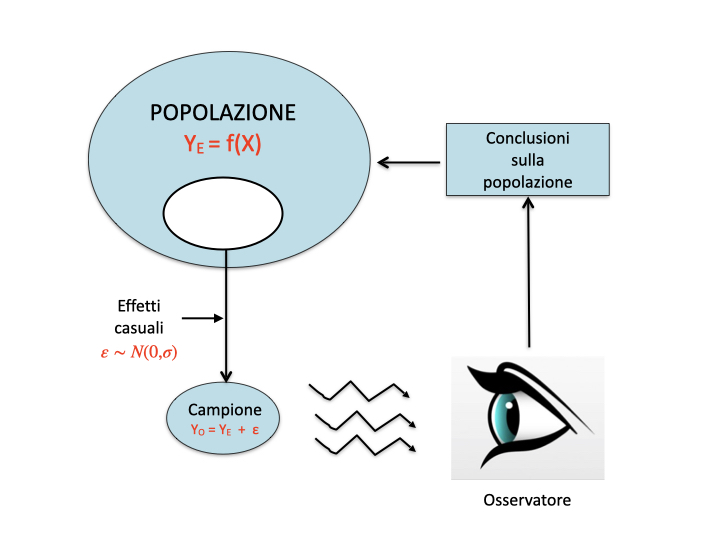
\includegraphics[width=0.75\linewidth]{_images/InferenceProcess} 

}

\caption{Osservazioni sperimentali e meccanismi perturbativi}\label{fig:figName61}
\end{figure}

Riprendiamo l'esempio relativo ad un pozzo inquinato da un erbicida a concentrazione pari a 120 \(mg/L\) (Capitolo 5), misurata tramite uno strumento che, unitamente a tutte le altre fonti ignote di errore, produce un coefficiente di variabilità del 10\% (corrispondente ad una deviazione standard di 12 \(mg/L\)). Abbiamo visto che, immaginando di fare le analisi in triplicato, i risultati di questo esperimento possono essere simulati con il modello della media, come lo abbiamo descritto nel capitolo precedente, cioè \(Y_O = Y_E + \varepsilon\), con \(\varepsilon \sim N(0, \sigma)\), \(Y_E = 120\) e \(\sigma = 12\).

Nell'esempio 5.3, la simulazione di Monte Carlo ha portato ai seguenti risultati: 105,5, 123,3 e 133,01 mg/L. Se adattiamo il ``modello della media'' a questo set di dati otteniamo un valore \(m = 120.62\), che differisce, anche se di poco, dal valore vero \(\mu = 120\). C'è quindi una discrasia tra la statistica campionaria e quella della popolazione (\(m \neq \mu\)).

\begin{Shaded}
\begin{Highlighting}[]
\FunctionTok{set.seed}\NormalTok{(}\DecValTok{1234}\NormalTok{)}
\NormalTok{Y\_E }\OtherTok{\textless{}{-}} \DecValTok{120}
\NormalTok{epsilon }\OtherTok{\textless{}{-}} \FunctionTok{rnorm}\NormalTok{(}\DecValTok{3}\NormalTok{, }\DecValTok{0}\NormalTok{, }\DecValTok{12}\NormalTok{)}
\NormalTok{Y\_O }\OtherTok{\textless{}{-}}\NormalTok{ Y\_E }\SpecialCharTok{+}\NormalTok{ epsilon}

\CommentTok{\# Fitting the ’model of the mean’ to the observed results}
\NormalTok{mod }\OtherTok{\textless{}{-}} \FunctionTok{lm}\NormalTok{(Y\_O }\SpecialCharTok{\textasciitilde{}} \DecValTok{1}\NormalTok{)}
\FunctionTok{coef}\NormalTok{(mod)}
\DocumentationTok{\#\# (Intercept) }
\DocumentationTok{\#\#    120.6192}
\end{Highlighting}
\end{Shaded}

A questo punto rimettiamoci in una situazione reale: non sappiamo quale sia la concentrazione nel pozzo e cerchiamo di determinarla utilizzando i risultati dell'esperimento appena citato. In assenza di altre informazioni, è logico concludere che \(\mu = m\), cioè che la statistica della popolazione coincida con quella campionaria. Questo processo con il quale assegniamo alla popolazione il valore della statistica campionaria prende il nome di \textbf{stima puntuale}. È un processo legittimo, ma insufficiente, in quanto \(m \neq \mu\), il che non ci sorprende: non è ragionevole infatti pensare che un qualunque campione possa riflettere con esattezza le caratteristiche della popolazione che lo ha generato. La nostra stima dovrà quindi essere ben più prudenziale.

L'approccio tradizionale consiste nel determinare un un intervallo di valori, che sia in grado di ``catturare'' la statistica della popolazione con elevata confidenza e una bassa probabilità di errore (\textbf{stima per intervallo}). Tale intervallo è chiamato \textbf{Intervallo di confidenza} (Confidence Interval: CI) ed è basato sulle teorie di Karl Pearson (1857-1936), di suo figlio Egon Pearson (1895-1980) e di Jerzy Neyman (1894-1981), nonché sul lavoro di Ronald Fisher. Il CI è uno dei fondamenti della cosiddetta inferenza frequentista, che non è l'unico tipo di inferenza disponibile e non è esente da alcune incongruenze concettuali (vedi Morey et al., 2016). Tuttavia, è molto comune e ampiamente utilizzata nella maggior parte degli articoli scientifici. Il termine ``frequentista'' deriva dal fatto che l'IC è costruito considerando la variabilità delle stime campionarie quando gli esperimenti vengono ripetuti e la frequenza con cui vengono ottenute i valori `sbagliati'.

\hypertarget{ripetere-gli-esperimenti}{%
\section{Ripetere gli esperimenti}\label{ripetere-gli-esperimenti}}

Il nostro esperimento è solo simulato e possiamo quindi ripeterlo `gratuitamente' un numero anche molto elevato di volte, seguendo questa procedura:

\begin{enumerate}
\def\labelenumi{\arabic{enumi}.}
\tightlist
\item
  Ripetiamo l'estrazione precedente per 100'000 volte (in altre parole: immaginiamo di ripetere l'analisi chimica per 100'000 volte, sempre con tre repliche)
\item
  Otteniamo 100'000 medie
\item
  Calcoliamo la media delle medie e la deviazione standard delle medie
\end{enumerate}

\begin{Shaded}
\begin{Highlighting}[]
\CommentTok{\# Code box 6.2}

\CommentTok{\# Monte Carlo simulation \#1}
\NormalTok{nrep }\OtherTok{\textless{}{-}} \DecValTok{3}
\NormalTok{mean }\OtherTok{\textless{}{-}} \DecValTok{120}
\NormalTok{sigma }\OtherTok{\textless{}{-}} \DecValTok{12}
\FunctionTok{set.seed}\NormalTok{(}\DecValTok{1234}\NormalTok{)}
\NormalTok{result }\OtherTok{\textless{}{-}} \FunctionTok{rep}\NormalTok{(}\DecValTok{0}\NormalTok{, }\DecValTok{100000}\NormalTok{)}
\ControlFlowTok{for}\NormalTok{ (i }\ControlFlowTok{in} \DecValTok{1}\SpecialCharTok{:}\DecValTok{100000}\NormalTok{)\{}
\NormalTok{  sample }\OtherTok{\textless{}{-}} \FunctionTok{rnorm}\NormalTok{(nrep, mean, sigma)}
\NormalTok{  mod }\OtherTok{\textless{}{-}} \FunctionTok{lm}\NormalTok{(sample }\SpecialCharTok{\textasciitilde{}} \DecValTok{1}\NormalTok{)}
\NormalTok{  result[i] }\OtherTok{\textless{}{-}} \FunctionTok{coef}\NormalTok{(mod)}
\NormalTok{\}}

\CommentTok{\# Characterising the population of estimates}
\FunctionTok{min}\NormalTok{(result)}

\DocumentationTok{\#\# [1] 90.14123}

\FunctionTok{max}\NormalTok{(result)}

\DocumentationTok{\#\# [1] 149.0346}

\NormalTok{result[result }\SpecialCharTok{==} \DecValTok{120}\NormalTok{]}

\DocumentationTok{\#\# numeric(0)}

\FunctionTok{mean}\NormalTok{(result)}

\DocumentationTok{\#\# [1] 120.0341}

\FunctionTok{sd}\NormalTok{(result)}

\DocumentationTok{\#\# [1] 6.939063}
\end{Highlighting}
\end{Shaded}

\normalsize

Alla fine del processo ci troviamo con una popolazione di medie, che viene detta distribuzione campionaria (\textbf{sampling distribution}); si tratta di un `oggetto' abbastanza `teorico', ma fondamentale per la statistica frequentista, perché caratterizza la variabilità dei risultati di un esperimento, e quindi la sua riproducibilità.

Notiamo che:

\begin{enumerate}
\def\labelenumi{\arabic{enumi}.}
\tightlist
\item
  La media delle medie è praticamente coincidente con \(\mu\), la verità `vera'. Ciò conferma che la stima puntuale \(m\) è uno stimatore non distorto di \(\mu\), perché tende a convergere su \(\mu\) quando il numero di repliche tende a diventare molto elevato;
\item
  La deviazione standard delle medie è pari a 6.939063 e prende il nome di \textbf{errore standard} (SE).
\end{enumerate}

Quest'ultima statistica è di importanza fondamentale, in quanto caratterizza la replicabilità di un esperimento, ovvero la sua precisione. Più è alto l'errore standard, più è incerta la stima e più è alta la sua variabilità in caso di esperimenti ripetuti.

Inoltre, possiamo osservare che il 2.5° e il 97.5° percentile sono, rispettivamente:

\begin{Shaded}
\begin{Highlighting}[]
\FunctionTok{quantile}\NormalTok{(result, }\AttributeTok{probs =}\FunctionTok{c}\NormalTok{(}\FloatTok{0.025}\NormalTok{, }\FloatTok{0.975}\NormalTok{))}
\DocumentationTok{\#\#     2.5\%    97.5\% }
\DocumentationTok{\#\# 106.4884 133.6434}
\end{Highlighting}
\end{Shaded}

Possiamo quindi dire che, ripetendo un esperimento un numero elevatissimo di volte, il 95\% dei risultati sono contenuti in un intervallo ben definito, che comprende al suo interno il valore `vero' della statistica da stimare.

\hypertarget{la-sampling-distribution-teorica}{%
\section{La `sampling distribution' teorica}\label{la-sampling-distribution-teorica}}

La \emph{sampling distribution} definita più sopra è puramente empirica e sarebbe molto utile poterla descrivere con una funzione di densità formale. Se discretizziamo il vettore `result' e riportiamo le frequenze su un grafico a barre (Fig. \ref{fig:figName62} ), vediamo con chiarezza che la \emph{sampling distribution} empirica somiglia molto ad una distribuzione normale, con media pari a 120 e deviazione standard pari a 6.94.

\begin{figure}

{\centering 
\includegraphics[width=0.75\linewidth]{_main_files/figure-latex/figName62-1} 

}

\caption{Empirical distribution of 100,000 sample estimates (n = 3), drawn from a Gaussian population with mean = 120 and SD = 12. The solid line shows the theoretical Gaussian PDF, with mean = 120 and SD = 6.94}\label{fig:figName62}
\end{figure}

Questa somiglianza può essere spiegato in base al teorema centrale del limite (o teorema del limite centrale), che teorizza che, qualunque sia la popolazione di partenza, molte statistiche campionarie, tra cui la media, calcolate su campioni casuali ed indipendenti, tendono a distribuirsi in modo approssimativamente normale, con una media pari alla corrispondente statistica della popolazione\footnote{Il teorema centrale del limite vale per campioni di dimensione elevata, composti da almeno 20-25 unità}.

Ammettendo che la \emph{sampling distribution} fosse Gaussiana, l'intervallo di cui abbiamo parlato poco sopra potrebbe essere individuato facilmente considerando un multiplo dell'errore standard, come \(\mu - k \times SE\) e \(\mu + k \times SE\) (Fig. \ref{fig:figName62b}). Inoltre, \(k\) sarebbe pari al 97.5° percentile di una distribuzione gaussiana standardizzata (ovvero una distribuzione gaussiana con media uguale a 0 e deviazione standard pari a 1), che è prossimo a 2 (con R: \texttt{qnorm(0,975)\ =\ 1.960}). Sfortunatamente, nella maggior parte dei casi, la distribuzione campionaria è solo approssimativamente gaussiana, quindi \(k\) deve essere determinato in modo diverso, come vedremo in seguito.

\begin{figure}

{\centering 
\includegraphics[width=0.75\linewidth]{_main_files/figure-latex/figName62b-1} 

}

\caption{A gaussian sampling distribution with a mean of 120 and standard deviation equal to 6.94 (n = 3); the red interval contains 95\% of our sample means and it is obtained by adding/subtracting to/from 120 a value equal to, approximately, twice the standard error}\label{fig:figName62b}
\end{figure}

\hypertarget{lintervallo-di-confidenza-frequentista}{%
\section{L'intervallo di confidenza frequentista}\label{lintervallo-di-confidenza-frequentista}}

Come abbiamo detto, l'intervallo menzionato in precedenza contiene il 95\% delle stime campionarie e, di conseguenza, soddisfa la seguente espressione:

\[P \left[ \mu - k \times SE  \leq m \leq \mu + k \times SE \right] = 0.95\]

Con semplici passaggi algebrici (sottraiamo \(\mu\) ed \(m\) da tutti i termini, moltiplichiamo per \(-1\) e riorganizziamo l'espressione), possiamo ricavare la seguente:

\[P \left[ m - k \times SE \leq \mu \leq m + k \times SE \right] = 0.95\]

che è di estrema importanza, in quanto esprime il concetto che, \textbf{se facciamo un esperimento ed otteniamo una media pari ad \(m\) e scegliamo accuratamente \(k\), possiamo costruire un intervallo di confidenza intorno alla nostra stima, pari a \(k\) volte l'errore standard e tale da contenere la media vera \(\mu\) con una probabilità del 95\%}. Questa espressione costituisce l'euristica più utilizzata per costruire l'\textbf{intervallo di confidenza}, anche se dobbiamo capire come ottenere SE e k.

\hypertarget{come-otteniamo-lerrore-standard}{%
\section{Come otteniamo l'errore standard?}\label{come-otteniamo-lerrore-standard}}

In alcuni casi, l'errore standard può essere ottenuto tramite semplici regole (Cochran, 1950), a partire dalla deviazione standard della popolazione di partenza. Ad esempio, nel caso della media campionaria, l'errore standard (SEM: Standard Error of a Mean) può essere ottenuto con la legge di propagazione degli errori (vedi capitolo 3.3):

\[\textrm{SEM}  = \frac{\sigma}{\sqrt n}\]

Nell'esempio precedente, l'errore standard è \(12/\sqrt{3} = 6,928\), molto vicino alla deviazione standard della distribuzione campionaria empirica.

Allo stesso modo, è possibile dimostrare che l'errore standard della differenza tra le medie di due campioni (SED: Standard Error of a Difference) indipendenti con numerosità, rispettivamente, pari a \(n_1\) ed \(n_2\), estratti da due popolazioni con la stessa varianza e la stessa media è:

\[\textrm{SED}  =  \sqrt{ \frac{\sigma^2}{n_1} + \frac{\sigma^2}{n_2}}\]

A parte questi due semplici casi, calcolare manualmente l'errore standard è difficile, ma, fortunatamente, possiamo utilizzare quelli prodotti dal software statistico in nostra vece. In particolare, per i modelli ottenuti con la funzione \texttt{lm()} o con altre funzioni di \emph{fitting} in R, gli errori standard per le stime dei parametri possono essere ricavati con la funzione \texttt{summary()}, passando l'oggetto che risulta dal \emph{fitting} come argomento. Ad esempio, riconsideriamo i dati dell'esperimento varietale a randomizzazione completa con tre repliche e quattro genotipi di avena, denominati A, B, C e D (Esempio 4.3). Se adattiamo ai risultati un semplice modello ANOVA ad una via (\(Y_i = \mu + \alpha_j + \varepsilon_i\)), le stime dei parametri con i relativi errori standard possono essere ottenute come mostrato nel riquadro sottostante.

\begin{Shaded}
\begin{Highlighting}[]
\CommentTok{\# Standard errors for parameter estimates}
\CommentTok{\# Input the data and fit the model (as in Chapter 4)}
\FunctionTok{library}\NormalTok{(statforbiology)}
\NormalTok{dataset }\OtherTok{\textless{}{-}} \FunctionTok{getAgroData}\NormalTok{(}\StringTok{"Oat1L"}\NormalTok{)}
\NormalTok{mod6}\FloatTok{.1} \OtherTok{\textless{}{-}} \FunctionTok{lm}\NormalTok{(Yield }\SpecialCharTok{\textasciitilde{}}\NormalTok{ Genotype, }\AttributeTok{data =}\NormalTok{ dataset)}
\CommentTok{\# Derive estimates and standard errors}
\FunctionTok{summary}\NormalTok{(mod6}\FloatTok{.1}\NormalTok{)}
\DocumentationTok{\#\# }
\DocumentationTok{\#\# Call:}
\DocumentationTok{\#\# lm(formula = Yield \textasciitilde{} Genotype, data = dataset)}
\DocumentationTok{\#\# }
\DocumentationTok{\#\# Residuals:}
\DocumentationTok{\#\#      Min       1Q   Median       3Q      Max }
\DocumentationTok{\#\# {-}0.17333 {-}0.08917  0.01833  0.07417  0.16333 }
\DocumentationTok{\#\# }
\DocumentationTok{\#\# Coefficients:}
\DocumentationTok{\#\#             Estimate Std. Error t value Pr(\textgreater{}|t|)    }
\DocumentationTok{\#\# (Intercept)  4.58000    0.07566  60.531 6.17e{-}12 ***}
\DocumentationTok{\#\# GenotypeB   {-}1.02667    0.10700  {-}9.595 1.16e{-}05 ***}
\DocumentationTok{\#\# GenotypeC   {-}0.49667    0.10700  {-}4.642  0.00166 ** }
\DocumentationTok{\#\# GenotypeD    0.01667    0.10700   0.156  0.88008    }
\DocumentationTok{\#\# {-}{-}{-}}
\DocumentationTok{\#\# Signif. codes:  0 \textquotesingle{}***\textquotesingle{} 0.001 \textquotesingle{}**\textquotesingle{} 0.01 \textquotesingle{}*\textquotesingle{} 0.05 \textquotesingle{}.\textquotesingle{} 0.1 \textquotesingle{} \textquotesingle{} 1}
\DocumentationTok{\#\# }
\DocumentationTok{\#\# Residual standard error: 0.1311 on 8 degrees of freedom}
\DocumentationTok{\#\# Multiple R{-}squared:  0.9412, Adjusted R{-}squared:  0.9192 }
\DocumentationTok{\#\# F{-}statistic: 42.71 on 3 and 8 DF,  p{-}value: 2.866e{-}05}
\end{Highlighting}
\end{Shaded}

\hypertarget{come-otteniamo-il-moltiplicatore-k}{%
\section{\texorpdfstring{Come otteniamo il moltiplicatore \(k\)?}{Come otteniamo il moltiplicatore k?}}\label{come-otteniamo-il-moltiplicatore-k}}

Per selezionare il moltiplicatore \(k\), dobbiamo considerare il \emph{coverage} dell'intervallo di confidenza, ovvero la frequenza con cui esso ``cattura'' il valore reale della statistica della popolazione. Generalmente, maggiore è il valore di \(k\), maggiore è l'ampiezza dell'intervallo e maggiore è il \emph{coverage}. Le informazioni di letteratura suggeriscono un \emph{coverage} del 95\%, corrispondente a una probabilità di errore del 5\%; di conseguenza, dovremmo chiederci: quale valore di \(k\) consenta di raggiungere tale confidenza?

Abbiamo già visto che, se la \emph{sampling distribution} fosse veramente gaussiana, \(k\) sarebbe all'incirca uguale a 2. Per determinare il \emph{coverage} con questo valore di \(k\) possiamo utilizzare il metodo Monte Carlo; in relazione all'esempio iniziale, riguardante il pozzo inquinato con una sostanza erbicida, possiamo eseguire, ripetutamente, queste operazioni:

\begin{enumerate}
\def\labelenumi{\arabic{enumi}.}
\tightlist
\item
  campioniamo tre individui da una popolazione gaussiana, con media pari a 120 e deviazione standard pari a 12;
\item
  adattiamo a questi tre individui il modello della media per ottenere una stima della media dell'intero pozzo, insieme al suo errore standard;
\item
  costruiamo un CI, utilizzando come moltiplicatore \(k = 2\). Se tale CI contiene il valore reale di 120 mg/L, l'esito è positivo e quindi assegniamo al risultato il valore 1 e lo immagazziniamo nel vettore `result'. Altrimenti assegniamo il valore 0 (funzione \texttt{ifelse()});;
\item
  ripetiamo i passaggi da 1 a 3 almeno per 100.000 volte e contiamo il numero di successi.
\end{enumerate}

\begin{Shaded}
\begin{Highlighting}[]
\CommentTok{\# Code box 6.4}

\CommentTok{\# Monte Carlo simulation {-} 2}
\CommentTok{\# Coverage of a confidence interval }
\CommentTok{\# depending on the multiplier k}
\CommentTok{\# Sampling 3 reps from a gaussian with mean=120 and sd=12}
\NormalTok{mean }\OtherTok{\textless{}{-}} \DecValTok{120}
\NormalTok{sigma }\OtherTok{\textless{}{-}} \DecValTok{12}
\NormalTok{nrep }\OtherTok{\textless{}{-}} \DecValTok{3}
\CommentTok{\# nrep \textless{}{-} 20}
\NormalTok{k }\OtherTok{\textless{}{-}} \DecValTok{2}
\CommentTok{\# k \textless{}{-} qt(0.975, nrep {-} 1)}
\FunctionTok{set.seed}\NormalTok{(}\DecValTok{1234}\NormalTok{)}
\NormalTok{result }\OtherTok{\textless{}{-}} \FunctionTok{rep}\NormalTok{(}\DecValTok{0}\NormalTok{, }\DecValTok{100000}\NormalTok{)}
\ControlFlowTok{for}\NormalTok{ (i }\ControlFlowTok{in} \DecValTok{1}\SpecialCharTok{:}\DecValTok{100000}\NormalTok{)\{}
\NormalTok{  sample.i }\OtherTok{\textless{}{-}} \FunctionTok{rnorm}\NormalTok{(nrep, mean, sigma)}
\NormalTok{  mod }\OtherTok{\textless{}{-}} \FunctionTok{lm}\NormalTok{(sample.i }\SpecialCharTok{\textasciitilde{}} \DecValTok{1}\NormalTok{)}
\NormalTok{  m }\OtherTok{\textless{}{-}} \FunctionTok{coef}\NormalTok{(mod)}
\NormalTok{  se }\OtherTok{\textless{}{-}} \FunctionTok{summary}\NormalTok{(mod)}\SpecialCharTok{$}\NormalTok{coef[}\DecValTok{1}\NormalTok{,}\DecValTok{2}\NormalTok{]}
\NormalTok{  limInf }\OtherTok{\textless{}{-}}\NormalTok{ m }\SpecialCharTok{{-}}\NormalTok{ k }\SpecialCharTok{*}\NormalTok{ se}
\NormalTok{  limSup }\OtherTok{\textless{}{-}}\NormalTok{ m }\SpecialCharTok{+}\NormalTok{ k }\SpecialCharTok{*}\NormalTok{ se}
  \CommentTok{\# did we capture the mean?}
\NormalTok{  result[i] }\OtherTok{\textless{}{-}} \FunctionTok{ifelse}\NormalTok{(limInf }\SpecialCharTok{\textless{}} \DecValTok{120} \SpecialCharTok{\&}\NormalTok{ limSup }\SpecialCharTok{\textgreater{}} \DecValTok{120}\NormalTok{, }\DecValTok{1}\NormalTok{, }\DecValTok{0}\NormalTok{)}
\NormalTok{\}}
\FunctionTok{sum}\NormalTok{(result)}\SpecialCharTok{/}\DecValTok{100000}
\DocumentationTok{\#\# [1] 0.81708}
\end{Highlighting}
\end{Shaded}

Il box sovrastante mostra che, impostando \(k = 2\) si ottiene un \emph{coverage} molto basso (inferiore all'82\%), corrispondente a una probabilità di errore di quasi il 19\%, che è inaccettabile. Il problema è che la dimensione del campione è molto piccola e, pertanto, la distribuzione campionaria di \(m\) non è ben approssimata con una PDF gaussiana. Se la stessa simulazione viene eseguita con 20 repliche anziché 3, il \emph{coverage} aumenta al 94\% (provare per credere; basta cambiare la linea di codice \texttt{nrep\ \textless{}-\ 3} con \texttt{nrep\ \textless{}-\ 20}). In pratica, utilizzare \(k = 2\) è ritenuto accettabile solo quando la dimensione del campione è superiore a 20-25 unità.

Per piccoli campioni (e in generale), è possibile ottenere un \emph{coverage} esatto del 95\% utilizzando il 97,5° percentile della distribuzione t di Student. Per ottenere questo valore, si può utilizzare la funzione \texttt{qt()} in R, che richiede, come minimo, due argomenti: il primo è il percentile desiderato, mentre il secondo rappresenta il numero di gradi di libertà per l'errore standard. Nel nostro esempio abbiamo tre repliche, quindi il numero di DF è 3 - 1 = 2 e il 97.5-esimo percentile della distribuzione t di Student è pari a \texttt{qt(0,975,\ 2)} = 4,303, molto più alto di 2. In genere, il 97,5-esimo percentile della distribuzione t di Student diminuisce all'aumentare del numero di gradi di libertà, tendendo ad 1,96, quando il numero di DF tende a \(\infty\). Se utilizziamo il codice sovrastante e sostituiamo alla linea \texttt{k\ \textless{}-\ 2}, il comando \texttt{k\ \textless{}-\ qt(0.975,\ nrep\ -\ 1)} possiamo confermare che il \emph{coverage} diviene quasi esattamente del 95\% (quasi, poiché il numero di simulazioni è molto alto, ma non infinito).

Se necessario, possiamo anche costruire un intervallo di confidenza del 99\%, che riduce il rischio di errore all'1\%. Basta utilizzare il 99,5° percentile di una distribuzione t di Student. In generale, se \(\alpha\) è il livello di confidenza desiderato, il percentile corrispondente è \(q_{\alpha} = 1 - (1 - \alpha/2)\) (quindi \(q_{0.05} = 1-(1-0.95)/2=0.975\) e \(q_{0.99} =1-(1-0,99)/2=0.995)\).

\hypertarget{gli-intervalli-di-confidenza-in-pratica}{%
\section{Gli intervalli di confidenza in pratica}\label{gli-intervalli-di-confidenza-in-pratica}}

\hypertarget{esempio-6.1-ic-per-una-media-campionaria}{%
\subsection{Esempio 6.1: IC per una media campionaria}\label{esempio-6.1-ic-per-una-media-campionaria}}

Immaginiamo di aver condotto un esperimento misurativo per determinare la resa media dei girasoli in un macro-ambiente dell'Italia centrale. Abbiamo quindi selezionato venti campi casuali in questo macro-ambiente ed abbiamo determinato i valori di resa riportati nel riquadro sottostante; sulla base di questi risultati, qual è la resa media nell'intero macro-ambiente?
In questo esempio, la media campionaria è \(m = 58,68\) ed è una stima puntuale affidabile della resa media nell'intero macro-ambiente. Per calcolare il CI, dobbiamo determinare:
1. l'errore standard, che può essere facilmente calcolato utilizzando la semplice equazione riportata più sopra (\(\textrm{SEM} = {\sigma}/{\sqrt n}\)). La deviazione standard della popolazione \(\sigma\) è ignota, ma possiamo sostituirla con la deviazione standard del campione, che è 3,47 (principio del `plug-in');
2. Il moltiplicatore \(k\), pari al 97,5° percentile della distribuzione t di Student (ovvero, 2,09).
Di conseguenza, i due limiti dell'intervallo di confidenza sono rispettivamente 58,68 - 2,09 \(\times\) 0,775 = 57,1 e 58,68 + 2,09 \(\times\) 0,775 = 60,3. La conclusione è che, con un livello di confidenza del 95\%, la resa media nel macro-ambiente rientra nell'intervallo tra 57,1 e 60,3.

\begin{Shaded}
\begin{Highlighting}[]
\CommentTok{\# Example 6.1}
\CommentTok{\# Confidence interval for a sample mean}
\CommentTok{\# Input the sample and calculate the mean}
\NormalTok{Y }\OtherTok{\textless{}{-}} \FunctionTok{c}\NormalTok{(}\FloatTok{54.08}\NormalTok{, }\FloatTok{66.31}\NormalTok{, }\FloatTok{56.17}\NormalTok{, }\FloatTok{56.32}\NormalTok{, }\FloatTok{52.01}\NormalTok{, }\FloatTok{58.91}\NormalTok{, }\FloatTok{58.74}\NormalTok{, }\FloatTok{57.49}\NormalTok{,}
\FloatTok{59.57}\NormalTok{, }\FloatTok{61.71}\NormalTok{, }\FloatTok{56.89}\NormalTok{, }\FloatTok{54.82}\NormalTok{, }\FloatTok{56.88}\NormalTok{, }\FloatTok{60.05}\NormalTok{, }\FloatTok{59.39}\NormalTok{, }\FloatTok{57.19}\NormalTok{,}
\FloatTok{64.76}\NormalTok{, }\FloatTok{61.36}\NormalTok{, }\FloatTok{62.03}\NormalTok{, }\FloatTok{58.83}\NormalTok{)}
\NormalTok{m }\OtherTok{\textless{}{-}} \FunctionTok{mean}\NormalTok{(Y)}
\NormalTok{m}
\DocumentationTok{\#\# [1] 58.6755}
\DocumentationTok{\#\# [1] 58.6755}
\CommentTok{\# Calculate the standard error}
\NormalTok{s }\OtherTok{\textless{}{-}} \FunctionTok{sd}\NormalTok{(Y)}
\NormalTok{SEM }\OtherTok{\textless{}{-}}\NormalTok{ s}\SpecialCharTok{/}\FunctionTok{sqrt}\NormalTok{(}\FunctionTok{length}\NormalTok{(Y))}
\NormalTok{SEM}
\DocumentationTok{\#\# [1] 0.7754783}
\DocumentationTok{\#\# [1] 0.7754783}
\CommentTok{\# Determine the multiplier}
\NormalTok{k }\OtherTok{\textless{}{-}} \FunctionTok{qt}\NormalTok{(}\FloatTok{0.975}\NormalTok{, }\FunctionTok{length}\NormalTok{(Y) }\SpecialCharTok{{-}} \DecValTok{1}\NormalTok{)}
\NormalTok{k}
\DocumentationTok{\#\# [1] 2.093024}
\DocumentationTok{\#\# [1] 2.093024}
\CommentTok{\# Calculate the limits of the CI \# Lower limit}
\FunctionTok{mean}\NormalTok{(Y) }\SpecialCharTok{{-}}\NormalTok{ k }\SpecialCharTok{*}\NormalTok{ SEM}
\DocumentationTok{\#\# [1] 57.05241}
\DocumentationTok{\#\# [1] 57.05241}
\CommentTok{\# Higher limit mean(Y) + k * SEM \#\# [1] 60.29859}
\end{Highlighting}
\end{Shaded}

Più facilmente, possiamo pervenire allo stesso risultato stimando un modello della media, ed utilizzando la funzione \texttt{confint()}, come indicato nel riquadro sottostante.

\begin{Shaded}
\begin{Highlighting}[]
\CommentTok{\# Example 6.1 [continuation]}
\CommentTok{\# Retrieving confidence intervals from model fit}
\NormalTok{mod }\OtherTok{\textless{}{-}} \FunctionTok{lm}\NormalTok{(Y }\SpecialCharTok{\textasciitilde{}} \DecValTok{1}\NormalTok{)}
\FunctionTok{confint}\NormalTok{(mod)}
\DocumentationTok{\#\#                2.5 \%   97.5 \%}
\DocumentationTok{\#\# (Intercept) 57.05241 60.29859}
\end{Highlighting}
\end{Shaded}

\hypertarget{example-6.2-cis-for-model-parameters}{%
\subsection{Example 6.2: CIs for model parameters}\label{example-6.2-cis-for-model-parameters}}

Lo stesso approccio del riquadro sovrastante può essere utilizzato praticamente con ogni altro modello in R. Ad esempio, riconsiderando i dati `Oat1L' dell' Esempio 4.3 e stimando un modello ANOVA ad una via come nel riquadro 4.3, gli intervalli di confidenza per le stime dei parametri possono essere ottenuti come nel riquadro 6.7.

\begin{Shaded}
\begin{Highlighting}[]
\CommentTok{\# Code box 6.7}
\CommentTok{\# Example 6.2}
\CommentTok{\# CIs for model parameters for the ’Oat1l’ data}
\CommentTok{\# Load libraries and data library(statforbiology)}
\NormalTok{dataset }\OtherTok{\textless{}{-}} \FunctionTok{getAgroData}\NormalTok{(}\StringTok{"Oat1L"}\NormalTok{)}
\CommentTok{\# Fit the model}
\NormalTok{mod6}\FloatTok{.1} \OtherTok{\textless{}{-}} \FunctionTok{lm}\NormalTok{(Yield }\SpecialCharTok{\textasciitilde{}}\NormalTok{ Genotype, }\AttributeTok{data =}\NormalTok{ dataset)}
\CommentTok{\# CIs for model parameters }
\FunctionTok{confint}\NormalTok{(mod6}\FloatTok{.1}\NormalTok{)}
\DocumentationTok{\#\#                  2.5 \%     97.5 \%}
\DocumentationTok{\#\# (Intercept)  4.4055191  4.7544809}
\DocumentationTok{\#\# GenotypeB   {-}1.2734199 {-}0.7799134}
\DocumentationTok{\#\# GenotypeC   {-}0.7434199 {-}0.2499134}
\DocumentationTok{\#\# GenotypeD   {-}0.2300866  0.2634199}
\end{Highlighting}
\end{Shaded}

\hypertarget{altri-approcci-per-il-calcolo-dei-ci}{%
\section{Altri approcci per il calcolo dei CI}\label{altri-approcci-per-il-calcolo-dei-ci}}

L'approccio proposto in questo capitolo si basa su due pre-requisiti fondamentali:

\begin{enumerate}
\def\labelenumi{\arabic{enumi}.}
\tightlist
\item
  la distribuzione campionaria sia gaussiana (almeno approssimativamente), e
\item
  sia possibile, in qualche modo, calcolare un errore standard affidabile.
\end{enumerate}

Nei casi in cui questi due pre-requisiti non siano soddisfatti, gli intervalli di confidenza possono essere determinati con altri approcci, come il metodo Monte Carlo (simile a quello utilizzato nel riquadro 6.2) o il metodo \emph{bootstrap} (Chernick, 2011). Inoltre, vale la pena menzionare l'``Intervallo Credibile'' (\emph{Credible Interval}), che è la controparte bayesiana dell'intervallo di confidenza frequentista (Kruschke, 2011).

Questi metodi fanno parte della cosiddetta \emph{computer intensive statistic} e possono essere molto utili in alcune circostanze, ma non saranno illustrati in dettaglio perché sono molto avanzati ed esulano dallo scopo di questo libro introduttivo.

\hypertarget{limitazioni-del-ci-frequentista}{%
\section{Limitazioni del CI frequentista}\label{limitazioni-del-ci-frequentista}}

L'intervallo di confidenza frequentista è ampiamente utilizzato nella letteratura scientifica, mentre la stima puntuale è spesso considerata inaccettabile. Ad esempio, le linee guida per gli autori di Weed Research, una rivista internazionale di alto livello nel campo delle scienze vegetali, affermano: ``Tutti i valori stimati (ad esempio, parametri del modello, medie, differenze, ecc.) devono essere presentati insieme a un'adeguata misura di variabilità sia nel testo, che nelle tabelle e nei grafici''. Gli intervalli di confidenza, molto spesso, sono presentati nella forma più semplice ``stima ± SE'', sebbene la copertura di tale intervallo sia piuttosto bassa. Basta comunque che il lettore sia avvisato sulla modalità utilizzata per la costruzione dell'intervallo presentato.

Per evitare gravi abusi interpretativi o di linguaggio, è necessario essere ben consapevoli dei limiti dell'intervallo di confidenza frequentista (Hastie et al., 2009), che deve essere sempre interpretato con riferimento ad una distribuzione campionaria, ovvero alle ipotetiche ripetizioni dello stesso esperimento con campioni diversi. Al contrario, è sbagliato interpretare il CI con riferimento ad ogni singolo esperimento; in altre parole, se il nostro intervallo di confidenza, determinato per uno specifico esperimento, va da 10 a 13, non è corretto affermare che il parametro incognito della popolazione è compreso tra 10 e 13 con una probabilità del 95\% perché ciò non è vero (ricordate che l'IC cambia a ogni tentativo di campionamento; vedere il riquadro 6.4 e vedere anche Morey et al., 2016). Possiamo invece affermare che, nel lungo periodo, ripetendo lo stesso esperimento e continuando a calcolare gli intervalli di confidenza nello stesso modo, la nostra probabilità di errore si mantiene entro il 5\%. Si tratta di una differenza piuttosto sottile, ma di fondamentale importanza!

\hypertarget{altre-letture-5}{%
\section{Altre letture}\label{altre-letture-5}}

\begin{enumerate}
\def\labelenumi{\arabic{enumi}.}
\tightlist
\item
  Chernick MR (2011) An Introduction to Bootstrap Methods with Applications to R. Wiley, USA
\item
  Cochran WG, Cox GM (1950) Experimental design. John Wiley \& Sons, Inc., USA
\item
  Hastie, T., Tibshirani, R., Friedman, J., 2009. The elements of statistical learning, Springer Series in Statistics. Springer Science + Business Media, California, USA.
\item
  Kruschke JK (2011) Doing bayesian data analyses. A tutorial with R and BUGS. Academic Press, Burlington, MA (USA)
\item
  Morey, RD, R Hoekstra, JN Rouder, MD Lee, E-J Wagenmakers, 2016. The fallacy of placing confidence in confidence intervals. Psychonomic Bulletin \& Review 23, 103--123
\end{enumerate}

\hypertarget{domande-ed-esercizi-4}{%
\section{Domande ed esercizi}\label{domande-ed-esercizi-4}}

\begin{enumerate}
\def\labelenumi{\arabic{enumi}.}
\tightlist
\item
  In un campo di frumento sono state campionate trenta aree di saggio di un metro quadrato ciascuna, sulle quali è stata determinata la produzione. La media delle trenta aree è stata di 6.2 t/ha, con una varianza pari a 0.9. Stimare la produzione dell'intero appezzamento.
\item
  Siamo interessati a conoscere il contenuto medio di nitrati dei pozzi della media valle del Tevere. Per questo organizziamo un esperimento, durante il quale campioniamo 20 pozzi rappresentativi, riscontrando le concentrazioni riportate di seguito. Stimare la concentrazione media per l'intera valle del Tevere
\end{enumerate}

\begin{verbatim}
38.3 38.6 38.1 39.9 36.3 41.6 37.0 39.8 39.1     
35.0 38.1 37.4 38.3 34.8 40.4 39.3 37.0 38.7    
38.2 38.4    
\end{verbatim}

\begin{enumerate}
\def\labelenumi{\arabic{enumi}.}
\setcounter{enumi}{2}
\tightlist
\item
  E'stata impostata una prova sperimentale per confrontare due varietà di mais, con uno schema sperimentale a blocchi randomizzati con tre repliche. La prima varietà ha mostrato produzioni di 14, 12, 15 e 13 t/ha, mentre la seconda varietà ha mostrato produzioni pari a 12, 11, 10.5 e 13 t/ha. Stimare le produzioni medie delle due varietà, nell'ambiente di studio.
\item
  Un campione di 400 insetti a cui è stato somministrato un certo insetticida mostra che 136 di essi sono sopravvissuti. Determinare un intervallo di confidenza con grado di fiducia del 95\% per la proporzione della popolazione insensibile al trattamento.
\item
  È stata studiata la risposta produttiva del sorgo alla concimazione azotata, con un esperimento i cui risultati sono riportati di seguito .Assumendo che la relazione sia lineare (retta), stimare la pendenza e l'intercetta della popolazione di riferimento, dalla quale è stato estratto il campione in studio. Utilizzare la funzione \texttt{lm(Yield\ \textasciitilde{}\ Dose)} ed estrarre gli errori standard con il metodo \texttt{summary()}.
\end{enumerate}

\begin{longtable}[]{@{}cc@{}}
\toprule()
Dose & Yield \\
\midrule()
\endhead
0 & 1.26 \\
30 & 2.50 \\
60 & 3.25 \\
90 & 4.31 \\
120 & 5.50 \\
\bottomrule()
\end{longtable}

\begin{enumerate}
\def\labelenumi{\arabic{enumi}.}
\setcounter{enumi}{5}
\tightlist
\item
  Utilizzando una simulazione Monte Carlo opportunamente pianificata, mostrare che la varianza del campione (uguale alla devianza divisa per il numero di individui meno uno) fornisce una stima più accurata della varianza della popolazione, rispetto allo scarto quadratico medio (devianza divisa per il numero di soggetti) che è invece uno stimatore distorto. Suggerimento: ricordare che uno stimatore accurato ha una distribuzione campionaria (\emph{sampling distribution}) il cui valore atteso coincide con il valore da stimare.
\end{enumerate}

\hypertarget{decisioni-ed-incertezza}{%
\chapter{Decisioni ed incertezza}\label{decisioni-ed-incertezza}}

Dovrebbero ormai essere chiari i motivi per cui i risultati di un esperimento non corrispondono alla verità vera e si presentano in modo diverso ogni volta che lo ripetiamo. Nel capitolo precedente abbiamo visto come è possibile (e necessario) esplicitare la nostra incertezza in relazione alla verità vera, aggiungendo alle nostre stime campionarie il cosiddetto \textbf{intervallo di confidenza}, basato sulla \emph{sampling distribution} della stima, che mostra come quest'ultima vari quando ripetiamo l'esperimento. Un approccio affine può essere utilizzato per prendere decisioni in presenza di incertezza, con un procedimento che si chiama \textbf{test d'ipotesi} ed è basato sul cosiddetto \textbf{P-level}. Anche per questo argomento, vediamo alcuni semplici, ma realistici, esempi.

\hypertarget{esempio-7.1-confronto-tra-due-genotipi}{%
\section{Esempio 7.1: Confronto tra due genotipi}\label{esempio-7.1-confronto-tra-due-genotipi}}

Immaginiamo che un ricercatore abbia testato la produzione di due genotipi (A e P) in un disegno sperimentale a randomizzazione completa, con cinque repliche (dieci parcelle in totale). I risultati ottenuti (q/ha) sono i seguenti:

Come al solito, l'analisi dei dati inizia con il calcolo delle più importanti statistiche descrittive per ogni campione, come abbiamo visto nel Capitolo 3. Trattandosi di una serie di misure quantitative, calcoliamo quindi media e deviazione standard, come indicato nel box sottostante.

\begin{Shaded}
\begin{Highlighting}[]
\CommentTok{\# Example 7.1}
\CommentTok{\# A comparison between two genotypes}

\CommentTok{\# Load the data}
\NormalTok{A }\OtherTok{\textless{}{-}} \FunctionTok{c}\NormalTok{(}\DecValTok{65}\NormalTok{, }\DecValTok{68}\NormalTok{, }\DecValTok{69}\NormalTok{, }\DecValTok{71}\NormalTok{, }\DecValTok{78}\NormalTok{)}
\NormalTok{P }\OtherTok{\textless{}{-}} \FunctionTok{c}\NormalTok{(}\DecValTok{80}\NormalTok{, }\DecValTok{81}\NormalTok{, }\DecValTok{84}\NormalTok{, }\DecValTok{88}\NormalTok{, }\DecValTok{94}\NormalTok{)}

\CommentTok{\# Descriptive statistics for A}
\NormalTok{m1 }\OtherTok{\textless{}{-}} \FunctionTok{mean}\NormalTok{(A)}
\NormalTok{s1 }\OtherTok{\textless{}{-}} \FunctionTok{sd}\NormalTok{(A)}
\NormalTok{n1 }\OtherTok{\textless{}{-}} \FunctionTok{length}\NormalTok{(A)}
\NormalTok{m1; s1; n1}
\DocumentationTok{\#\# [1] 70.2}
\DocumentationTok{\#\# [1] 4.868265}
\DocumentationTok{\#\# [1] 5}
\CommentTok{\# Descriptive statistics for P}
\NormalTok{m2 }\OtherTok{\textless{}{-}} \FunctionTok{mean}\NormalTok{(P)}
\NormalTok{s2 }\OtherTok{\textless{}{-}} \FunctionTok{sd}\NormalTok{(P)}
\NormalTok{n2 }\OtherTok{\textless{}{-}} \FunctionTok{length}\NormalTok{(P)}
\NormalTok{m2; s2; n2}
\DocumentationTok{\#\# [1] 85.4}
\DocumentationTok{\#\# [1] 5.727128}
\DocumentationTok{\#\# [1] 5}
\end{Highlighting}
\end{Shaded}

Vediamo che la media per il genotipo P è più alta della media per il genotipo A, ma tali medie campionarie non sono sufficienti per i nostri obiettivi. Il passo successivo è postulare un modello descrittivo per rappresentare il meccanismo tramite cui le nostre osservazioni (e altre osservazioni future) potrebbero essere originate. Tale modello dovrebbe tenere conto dell'effetto di una variabile predittiva, ovvero il genotipo. Un modello ragionevole è:

\[
Y_i = \mu + \delta_j + \varepsilon_{i}
\]

dove \(Y_i\) è la resa dell'i\textsuperscript{-esimo} grafico (\(i\) va da 1 a 10), \(\mu\) è la resa prevista per il genotipo A, mentre \(\delta_j\) è l'effetto del genotipo (con \(j\) che va da 1 a 2) che è vincolato a essere 0 per il primo genotipo (\(\delta_1 = 0\)) e, per il secondo genotipo, è uguale alla differenza di resa tra i due genotipi (\(\delta_2 = \mu_2 - \mu_1\)). Di conseguenza, la resa prevista per P è \(\mu_2 = \mu_1 + \delta_2\) e i residui \(\varepsilon_i\) rappresentano tutte le altre fonti sconosciute di variabilità, che sono indipendenti e specifiche per ogni grafico. I residui sono assunti come gaussiani, con media uguale a 0 e deviazione standard uguale a \(\sigma\). La scelta di usare \(\delta_2\) (differenze tra la seconda varietà è la prima) come parametro esplicito nel modello è puramente arbitraria: avremmo potuto anche includere \(\delta_1\) (differenze tra la prima varietà e la seconda) che sarebbe stata uguale a \(\delta_2\) in valore assoluto, ma con segno invertito e avrebbe reso \(\mu\) uguale alla media del secondo genotipo, invece che del primo.

La stima dei parametri del modello può essere eseguita utilizzando la funzione \texttt{lm()} in R, come mostrato nel Capitolo 4.

\begin{Shaded}
\begin{Highlighting}[]
\CommentTok{\# Example 7.1 [continuation]}

\CommentTok{\# Fitting a model with one nominal predictor}
\CommentTok{\# to the data at Code box 7.1}

\NormalTok{yield }\OtherTok{\textless{}{-}} \FunctionTok{c}\NormalTok{(A, P)}
\NormalTok{genotype }\OtherTok{\textless{}{-}} \FunctionTok{rep}\NormalTok{(}\FunctionTok{c}\NormalTok{(}\StringTok{"A"}\NormalTok{, }\StringTok{"P"}\NormalTok{), }\AttributeTok{each =} \DecValTok{5}\NormalTok{)}
\NormalTok{mod }\OtherTok{\textless{}{-}} \FunctionTok{lm}\NormalTok{(yield }\SpecialCharTok{\textasciitilde{}}\NormalTok{ genotype)}
\FunctionTok{summary}\NormalTok{(mod)}
\DocumentationTok{\#\# }
\DocumentationTok{\#\# Call:}
\DocumentationTok{\#\# lm(formula = yield \textasciitilde{} genotype)}
\DocumentationTok{\#\# }
\DocumentationTok{\#\# Residuals:}
\DocumentationTok{\#\#    Min     1Q Median     3Q    Max }
\DocumentationTok{\#\#  {-}5.40  {-}3.85  {-}1.30   2.15   8.60 }
\DocumentationTok{\#\# }
\DocumentationTok{\#\# Coefficients:}
\DocumentationTok{\#\#             Estimate Std. Error t value Pr(\textgreater{}|t|)    }
\DocumentationTok{\#\# (Intercept)   70.200      2.377  29.533 1.87e{-}09 ***}
\DocumentationTok{\#\# genotypeP     15.200      3.362   4.522  0.00195 ** }
\DocumentationTok{\#\# {-}{-}{-}}
\DocumentationTok{\#\# Signif. codes:  0 \textquotesingle{}***\textquotesingle{} 0.001 \textquotesingle{}**\textquotesingle{} 0.01 \textquotesingle{}*\textquotesingle{} 0.05 \textquotesingle{}.\textquotesingle{} 0.1 \textquotesingle{} \textquotesingle{} 1}
\DocumentationTok{\#\# }
\DocumentationTok{\#\# Residual standard error: 5.315 on 8 degrees of freedom}
\DocumentationTok{\#\# Multiple R{-}squared:  0.7188, Adjusted R{-}squared:  0.6836 }
\DocumentationTok{\#\# F{-}statistic: 20.45 on 1 and 8 DF,  p{-}value: 0.001945}
\FunctionTok{confint}\NormalTok{(mod)}
\DocumentationTok{\#\#                 2.5 \%   97.5 \%}
\DocumentationTok{\#\# (Intercept) 64.718691 75.68131}
\DocumentationTok{\#\# genotypeP    7.448258 22.95174}
\end{Highlighting}
\end{Shaded}

È importante notare che la deviazione standard residua (\(\sigma\)), con una terminologia confusa, è indicata come `errore standard residuo' (\(\sigma = 5,315\)) nell'output R. È anche importante notare che, in base al nostro modello, la deviazione standard dei residui è unica e comune a tutte le osservazioni e, pertanto, stiamo assumendo che l'effetto genotipo influenzi il livello di resa e non la sua variabilità tra le repliche. Tale ipotesi è chiamata \textbf{omoschedasticità} (od \textbf{omoscedasticità}) e dovrebbe essere attentamente verificata, come mostreremo più avanti in questo libro.

Gli errori standard per tutte le stime puntuali sono già disponibili nell'output di R: confermano che c'è una certa incertezza sulla reale differenza basata sulla popolazione \(\delta_2\), che dovrebbe essere compresa tra 7,45 e 22,95. Il fatto che l'intervallo di confidenza per \(\delta_2\) non contenga 0 è una prova indiretta che l'effetto genotipo è significativo.

\hypertarget{lipotesi-nulla}{%
\subsection{L'ipotesi `nulla'}\label{lipotesi-nulla}}

Dopo aver completato l'inferenza statistica, ci chiediamo se, a livello di popolazione, sia possibile concludere che il genotipo P è più produttivo del genotipo A, coerentemente con i risultati osservati nei due campioni. Non dimentichiamoci che i due campioni sono totalmente irrilevanti, perché vogliamo trarre conclusioni generali e non specifiche per il nostro esperimento. Dobbiamo quindi \textbf{trovare un metodo per decidere se il genotipo P, in generale, è più produttivo del genotipo A}, pur in presenza dell'incertezza legata all'errore sperimentale.

Innanzitutto, ricordiamo la logica Popperiana illustrata nel primo capitolo, secondo la quale nessun esperimento può dimostrare che un'ipotesi scientifica è vera, mentre è possibile dimostrare che essa è falsa. E'quindi conveniente porre l'ipotesi scientifica di nostro interesse (\(H_0\)) in modo che essa possa essere falsificata, cioè, ad esempio:

\[H_0: \delta_2 = 0\]

In altre parole, stiamo cercando di dimostrare che uno dei parametri stimati nel modello sia, in realtà, uguale a 0; questa ipotesi si chiama \textbf{ipotesi nulla} e, se riuscissimo a falsificarla, avremmo conseguito il nostro obiettivo, in totale coerenza con la logica Popperiana.

\hypertarget{il-test-di-t-wald-test}{%
\subsection{Il test di t (Wald test)}\label{il-test-di-t-wald-test}}

In practica, stiamo cercando di dimostrare che un parametro del modello è uguale a 0, quando, in realtà, la nostra stima puntuale è diversa da 0. È intuitivamente chiaro che un certo grado di discrepanza tra la realtà e l'osservazione è accettabile come caratteristica intrinseca del processo di campionamento, ma è anche chiaro che maggiore è la discrepanza, minore è la probabilità che l'ipotesi ``nulla'' sia vera. In particolare, la nostra intuizione è che un parametro è significativamente diverso da zero quando il suo valore è molto più grande dell'incertezza con cui lo abbiamo stimato.

Un statistica che risponde alla nostra esigenza è quella indicata di seguito:

\[T = \frac{d_2}{SE_{d_2}} = \frac{15.2}{3.362} = 4.521727\]

Se l'ipotesi nulla fosse vera, dovremmo osservare \(T = 0\), mentre abbiamo osservato \(T = 4,522\). Possiamo rifiutare il nullo? Non lo sappiamo, dipende da quanto è probabile ottenere un valore così discrepante quando il nullo è vero. Pertanto, dobbiamo chiederci: \textbf{qual è la distribuzione campionaria per \(T\) sotto l'ipotesi nulla?}

\hypertarget{simulazione-monte-carlo}{%
\subsection{Simulazione Monte Carlo}\label{simulazione-monte-carlo}}

Per rispondere a questa domanda, supponiamo che l'ipotesi nulla sia vera. In questo caso, immaginiamo che le nostre dieci parcelle siano tutte estratte da una sola popolazione di parcelle con media e deviazione standard stimate (stima puntuale) come segue:

\begin{Shaded}
\begin{Highlighting}[]
\CommentTok{\# Example 7.1 [ continuation]}
\CommentTok{\# We assume a single group, with no genotype distinction}
\CommentTok{\# and calculate the descriptive statistics}
\NormalTok{mu }\OtherTok{\textless{}{-}} \FunctionTok{mean}\NormalTok{(yield)}
\NormalTok{devStAP }\OtherTok{\textless{}{-}} \FunctionTok{sd}\NormalTok{(}\FunctionTok{c}\NormalTok{(A, P))}
\NormalTok{mu; devStAP}
\DocumentationTok{\#\# [1] 77.8}
\DocumentationTok{\#\# [1] 9.44928}
\end{Highlighting}
\end{Shaded}

Prendiamo quindi questa popolazione normale, con \(\mu = 77.8\) e \(\sigma = 9.45\), ed utilizziamo un generatore di numeri casuali gaussiani per estrarre numerose (100'000) coppie di campioni, calcolando, per ogni coppia, il valore T, come abbiamo fatto con la nostra coppia iniziale. Il codice da utilizzare in R per le simulazioni è il seguente:

\begin{Shaded}
\begin{Highlighting}[]
\CommentTok{\# Example 7.1 [ continuation]}

\CommentTok{\# Building a sampling distribution for T}
\CommentTok{\# assuming that the null hypothesis is true}

\FunctionTok{set.seed}\NormalTok{(}\DecValTok{34}\NormalTok{)}
\NormalTok{result }\OtherTok{\textless{}{-}} \FunctionTok{rep}\NormalTok{(}\ConstantTok{NA}\NormalTok{, }\DecValTok{100000}\NormalTok{)}
\ControlFlowTok{for}\NormalTok{ (i }\ControlFlowTok{in} \DecValTok{1}\SpecialCharTok{:}\DecValTok{100000}\NormalTok{)\{}
\NormalTok{  epsilon }\OtherTok{\textless{}{-}} \FunctionTok{rnorm}\NormalTok{(}\DecValTok{10}\NormalTok{, }\DecValTok{0}\NormalTok{, devStAP)}
\NormalTok{  Yo }\OtherTok{\textless{}{-}}\NormalTok{ mu }\SpecialCharTok{+}\NormalTok{ epsilon}
\NormalTok{  mod }\OtherTok{\textless{}{-}} \FunctionTok{lm}\NormalTok{(Yo }\SpecialCharTok{\textasciitilde{}}\NormalTok{ genotype)}
\NormalTok{  d2 }\OtherTok{\textless{}{-}} \FunctionTok{coef}\NormalTok{(mod)[}\DecValTok{2}\NormalTok{]}
\NormalTok{  SE }\OtherTok{\textless{}{-}} \FunctionTok{summary}\NormalTok{(mod)}\SpecialCharTok{$}\NormalTok{coefficients[[}\DecValTok{2}\NormalTok{,}\DecValTok{2}\NormalTok{]]}
\NormalTok{  Ti }\OtherTok{\textless{}{-}}\NormalTok{ d2 }\SpecialCharTok{/}\NormalTok{ SE}
\NormalTok{  result[i] }\OtherTok{\textless{}{-}}\NormalTok{ Ti}
\NormalTok{\}}
\FunctionTok{mean}\NormalTok{(result) }
\DocumentationTok{\#\# 0.001230418}

\FunctionTok{min}\NormalTok{(result)}
\DocumentationTok{\#\# {-}9.988315}

\FunctionTok{max}\NormalTok{(result)}
\DocumentationTok{\#\# 9.993187}
\end{Highlighting}
\end{Shaded}

\begin{Shaded}
\begin{Highlighting}[]
\FunctionTok{mean}\NormalTok{(result) }
\DocumentationTok{\#\# [1] 0.001230418}
\FunctionTok{min}\NormalTok{(result)}
\DocumentationTok{\#\# [1] {-}9.988315}
\FunctionTok{max}\NormalTok{(result)}
\DocumentationTok{\#\# [1] 9.993187}
\end{Highlighting}
\end{Shaded}

Quali valori abbiamo ottenuto per \(T\)? In media, i valori sono prossimi a 0, come previsto, considerando che abbiamo simulato i risultati di esperimenti in cui \(\delta_2\) era assunto pari a 0. Tuttavia, notiamo anche valori piuttosto alti e bassi (vicini a 10 e -10), il che dimostra che le fluttuazioni del campionamento casuale possono anche portare a risultati molto ``strani''. Per il nostro esperimento reale abbiamo ottenuto \(T = 4,522\), sebbene il segno positivo sia solo un artefatto, legato al modo in cui abbiamo formulato il nostro modello: avremmo potuto ottenere anche \(T = -4,522\) se avessimo utilizzato \(\mu_2\) come parametro esplicito, invece di \(\mu_1\).

\textbf{Ronald Fisher ha proposto di rifiutare l'ipotesi nulla, in base alla probabilità di ottenere valori tanto `estremi' o più `estremi' di quello osservato, quando l'ipotesi nulla è vera}. Osservando il vettore ``result'', vediamo che la proporzione di valori inferiori a -4,521727 e superiori a 4,521727 è \(0,00095 + 0,00082 = 0,00177\). Questo è il cosiddetto \textbf{P-Level} o \textbf{P-value} (vedere il codice sottostante).

\vspace{12pt}

\begin{Shaded}
\begin{Highlighting}[]
\CommentTok{\# Example 7.1 [ continuation]}
\CommentTok{\# P{-}value with Monte Carlo simulation}
\NormalTok{T\_obs }\OtherTok{\textless{}{-}} \FloatTok{4.521727}
\NormalTok{upperTail }\OtherTok{\textless{}{-}} \FunctionTok{length}\NormalTok{(result[result }\SpecialCharTok{\textgreater{}}\NormalTok{ T\_obs]) }\SpecialCharTok{/} \DecValTok{100000}
\NormalTok{lowerTail }\OtherTok{\textless{}{-}} \FunctionTok{length}\NormalTok{(result[result }\SpecialCharTok{\textless{}} \SpecialCharTok{{-}}\NormalTok{ T\_obs]) }\SpecialCharTok{/}\DecValTok{100000} 
\NormalTok{upperTail }\SpecialCharTok{+}\NormalTok{ lowerTail}
\DocumentationTok{\#\# [1] 0.00177}
\end{Highlighting}
\end{Shaded}

Ora proviamo a riassumere. Abbiamo visto che, quando l'ipotesi nulla è vero, la distribuzione campionaria di \(T\) contiene una percentuale molto bassa di valori al di fuori dell'intervallo da -4,522 a 4,522. Pertanto, la nostra osservazione rientra in un intervallo molto improbabile, che ha scarsissima probabilità di verificarsi (P-value = 0.0017); \textbf{il P-value di riferimento per il rigetto della nulla è 0,05}, quindi, coerentemente, la rigettiamo. Lo facciamo perché, se l'ipotesi nulla fosse vera, avremmo ottenuto un risultato molto improbabile; in altre parole, l'e nostre prove scientifiche contro il valore nullo 'evidenza scientifica contro l'ipotesi nulla è sufficientemente forte da permetterci di rigettarla.

\hypertarget{una-soluzione-formale}{%
\subsection{Una soluzione formale}\label{una-soluzione-formale}}

Calcolare il P-value poco sopra ha richiesto di costruire una \emph{sampling distribution} empirica con una serie di simulazioni Monte Carlo, piuttosto `costose' in termini di tempo di calcolo. Allora è opportuno chiedersi: esiste una Funzione di Densità di Probabilità (PDF) formale che possiamo utilizzare al posto \emph{sampling distribution} empirica? Se prendiamo il vettore `result' e lo `discretizziamo', riportandolo in un istogramma (Fig. \ref{fig:figName71}) possiamo vedere che la distribuzione empirica non assomiglia del tutto ad una gaussiana standardizzata, ma può essere descritta con un altro tipo di distribuzione, ovvero la `t di Student', con otto gradi di libertà (ovvero la somma dei gradi di libertà dei due campioni)\footnote{La distribuzione t di Student fu ideata dallo `studente' William Sealy Gosset (1876 - 1937), che utilizzava questo pseudonimo nei suoi articoli scientifici mentre lavorava alla Guinness Brewery di Dublino. E' simile a una distribuzione gaussiana standardizzata, ma con code più alte, cioè con una maggiore probabilità di ottenere outliers, sia positivi, che negativi. L'altezza delle code è inversamente proporzionale al parametro \(\nu\) (il numero di DF), in modo che questa distribuzione tende ad una gaussiana quando \(\nu\) tende ad infinito}.

\begin{verbatim}
## Warning: Removed 25 rows containing non-finite outside the scale range
## (`stat_bin()`).
## Warning: Removed 32 rows containing missing values or values outside the scale
## range (`geom_bar()`).
\end{verbatim}

\begin{figure}

{\centering 
\includegraphics[width=0.85\linewidth]{_main_files/figure-latex/figName71-1} 

}

\caption{Empirical sampling distribution for the T statistic, compared to a standardised gaussian (blue line) and a Student's t distribution with 8 degrees of freedom (red line). The observed T-values have been highlighted and the total probability (area-under-the-curve) of sampling outside the interval from -4.522 to 4.522 represents the P-value}\label{fig:figName71}
\end{figure}

Di conseguenza, possiamo utilizzare la distribuzione t di Student per calcolare il \emph{P-value}, come mostrato nel riquadro sottostante. Invece che sommare le probabilità di ottenere valori superiori a 4.522 e di ottenere valori inferiori a -4.522, possiamo anche moltiplicare per due la probabilità di ottenere valori superiori al valore assoluto del T osservata. Infatti, la distribuzione di t di Student è simmetrica, e quindi le due code sono uguali.

\vspace{12pt}

\begin{Shaded}
\begin{Highlighting}[]
\CommentTok{\# Example 7.1 [continuation\}}

\CommentTok{\# P{-}value from the Student\textquotesingle{}s t distribution}

\FunctionTok{pt}\NormalTok{(T\_obs, }\AttributeTok{df=}\DecValTok{8}\NormalTok{, }\AttributeTok{lower.tail =} \ConstantTok{FALSE}\NormalTok{) }\CommentTok{\# probability that T \textgreater{} 4.522}
\DocumentationTok{\#\# [1] 0.0009727353}
\FunctionTok{pt}\NormalTok{(}\SpecialCharTok{{-}}\NormalTok{T\_obs, }\AttributeTok{df=}\DecValTok{8}\NormalTok{) }\CommentTok{\# probability that T \textless{} {-}4.522}
\DocumentationTok{\#\# [1] 0.0009727353}
\DecValTok{2} \SpecialCharTok{*} \FunctionTok{pt}\NormalTok{(}\FunctionTok{abs}\NormalTok{(T\_obs), }\AttributeTok{df=}\DecValTok{8}\NormalTok{, }\AttributeTok{lower.tail =}\NormalTok{ F) }\CommentTok{\# P{-}value}
\DocumentationTok{\#\# [1] 0.001945471}
\end{Highlighting}
\end{Shaded}

Vediamo che il P-level ottenuto formalmente è simile a quello ottenuto empiricamente, ma, rispetto a quest'ultimo, è più preciso, in quanto con la simulazione di Monte Carlo non abbiamo potuto considerare, come avremmo dovuto, un numero infinito di repliche dell'esperimento.

Per concludere questa sezione, dobbiamo precisare che \textbf{l'impiego di una \emph{sampling distribution} formale richiede che siano verificate due condizioni di base}:

\begin{enumerate}
\def\labelenumi{\arabic{enumi}.}
\tightlist
\item
  i residui sono campionati da una distribuzione normale (normalità);
\item
  la deviazione standard è unica e non è influenzata dal trattamento sperimentale (omoschedasticità).
\end{enumerate}

Avrete infatti notato che queste due condizioni erano `incapsulate' nella simulazione Monte Carlo che abbiamo eseguito in precedenza per ottenere la \emph{sampling distribution} empirica di T. Se le due ipotesi non fossero rispettate, la distribuzione t di Student non rappresenterebbe esattamente la \emph{sampling distribution} della statistica T e, di conseguenza, il P-level non sarebbe valido. Più avanti in questo libro vedremo come è possibile verificare che le due assunzioni di base siano effettivamente rispettate.

\hypertarget{altri-test-di-t}{%
\section{Altri test di t}\label{altri-test-di-t}}

\hypertarget{il-test-t-di-student}{%
\subsection{Il test t di Student}\label{il-test-t-di-student}}

Il test t che abbiamo appena mostrato è utilizzato come supporto alle procedure di \emph{model fitting} (Wald test) e permette di verificare l'ipotesi che uno dei parametri stimati sia significativamente diverso da 0. Il test t di Student è invece una tecnica tradizionale di analisi dei dati (risale al 1908) per il confronto tra due medie campionarie, senza alcun legame col \emph{model fitting}. Sebbene, al giorno d'oggi il test t di Student debba essere considerato un po' obsoleto, è comunque opportuno conoscere come questa procedura possa essere eseguita in R, con la funzione \texttt{t.test()}. Il box sottostante mostra che i risultati che si ottengono sono identici a quelli ottenuti nella sezione precedente.

\vspace{12pt}

\begin{Shaded}
\begin{Highlighting}[]
\CommentTok{\# Example 7.1 [continuation]}

\CommentTok{\# Traditional Student\textquotesingle{}s t{-}test with R}

\FunctionTok{t.test}\NormalTok{(A, P, }\AttributeTok{var.equal =} \ConstantTok{TRUE}\NormalTok{)}
\DocumentationTok{\#\# }
\DocumentationTok{\#\#  Two Sample t{-}test}
\DocumentationTok{\#\# }
\DocumentationTok{\#\# data:  A and P}
\DocumentationTok{\#\# t = {-}4.5217, df = 8, p{-}value = 0.001945}
\DocumentationTok{\#\# alternative hypothesis: true difference in means is not equal to 0}
\DocumentationTok{\#\# 95 percent confidence interval:}
\DocumentationTok{\#\#  {-}22.951742  {-}7.448258}
\DocumentationTok{\#\# sample estimates:}
\DocumentationTok{\#\# mean of x mean of y }
\DocumentationTok{\#\#      70.2      85.4}
\end{Highlighting}
\end{Shaded}

\hypertarget{il-test-di-welch}{%
\subsection{Il test di Welch}\label{il-test-di-welch}}

Anche il test di t di Student richiede l'omoschedasticità dei dati e necessita dell'argomento \texttt{var.equal\ =\ TRUE}. Tuttavia, la funzione \texttt{t.test()} può essere facilmente estesa alle situazioni in cui i due campioni hanno varianze diverse, modificando il codice con l'argomento \texttt{var.equal\ =\ FALSE}. In questo modo viene eseguito il test di t eteroschedastico, noto anche come test di Welch. Grazie al suo maggiore livello di robustezza, il test di Welch è solitamente preferito al test t di Student ed è, quindi, l'opzione predefinita in R.

\vspace{12pt}

\begin{Shaded}
\begin{Highlighting}[]
\CommentTok{\# Code box 7.8}
\CommentTok{\# Example 7.1 [continuation]}

\CommentTok{\# Heteroscedastic t{-}test (Welch test) with R}

\FunctionTok{t.test}\NormalTok{(A, P, }\AttributeTok{var.equal =}\NormalTok{ F)}
\DocumentationTok{\#\# }
\DocumentationTok{\#\#  Welch Two Sample t{-}test}
\DocumentationTok{\#\# }
\DocumentationTok{\#\# data:  A and P}
\DocumentationTok{\#\# t = {-}4.5217, df = 7.7977, p{-}value = 0.002076}
\DocumentationTok{\#\# alternative hypothesis: true difference in means is not equal to 0}
\DocumentationTok{\#\# 95 percent confidence interval:}
\DocumentationTok{\#\#  {-}22.986884  {-}7.413116}
\DocumentationTok{\#\# sample estimates:}
\DocumentationTok{\#\# mean of x mean of y }
\DocumentationTok{\#\#      70.2      85.4}
\end{Highlighting}
\end{Shaded}

\hypertarget{il-test-di-t-appaiato}{%
\subsection{Il test di t appaiato}\label{il-test-di-t-appaiato}}

In alcuni casi, l'esperimento prevede due misure sullo stesso soggetto ed è finalizzato a verificare se esiste una differenza significativa tra la prima e la seconda misura. Ad esempio, immaginiamo di aver esaminato un campione di venti topi pesandoli all'inizio e alla fine di un certo programma alimentare; in questo modo,si viene ad avere, per ogni individuo, due misurazioni appaiate, per un totale di quaranta valori. In tali condizioni, le due misure non sono indipendenti tra di loro e dobbiamo necessariamente eseguire un test di t appaiato, impostando l'argomento \texttt{paired\ =\ TRUE}, come mostrato nel riquadro sottostante. Si noti che, anche se abbiamo 40 valori, il numero di gradi di libertà è 19, perché abbiamo solo 20 soggetti indipendenti e due misure per soggetto.

\hypertarget{differenze-generalizzate-tra-parametri}{%
\section{Differenze generalizzate tra parametri}\label{differenze-generalizzate-tra-parametri}}

Il test di Welch può essere generalizzato a qualunque situazione in cui abbiamo due stime indipendenti e vogliamo valutare se la loro differenza è significativa. Ad esempio, immaginiamo di aver stimato il tasso di crescita della barbabietola da zucchero con due diverse pratiche agronomiche e di aver ottenuto le stime \(\rho_1 = 0.22\) con un errore standard di 0.013 e \(\rho_2 = 0.31\) con un errore standard di 0.029. Il valore di T può essere ottenuto come:

\[T = \frac{0.31 - 0.22}{\sqrt{0.031^2 + 0.029^2}} = -2.12\]

Se la dimensione del campione è sufficientemente ampia e le due stime provengono da un ugual numero di soggetti, potremmo utilizzare un'approssimazione gaussiana per ottenere il P-value, come mostrato nel box sottostante.

\begin{Shaded}
\begin{Highlighting}[]
\CommentTok{\# Code box 7.10}

\CommentTok{\# Example 7.3}
\CommentTok{\# testing differences between model parameters}

\NormalTok{T\_obs }\OtherTok{\textless{}{-}}\NormalTok{ (}\FloatTok{0.22} \SpecialCharTok{{-}} \FloatTok{0.31}\NormalTok{)}\SpecialCharTok{/}\FunctionTok{sqrt}\NormalTok{(}\FloatTok{0.031}\SpecialCharTok{\^{}}\DecValTok{2} \SpecialCharTok{+} \FloatTok{0.029}\SpecialCharTok{\^{}}\DecValTok{2}\NormalTok{)}
\DecValTok{2} \SpecialCharTok{*} \FunctionTok{pnorm}\NormalTok{(}\FunctionTok{abs}\NormalTok{(T\_obs), }\AttributeTok{lower.tail =}\NormalTok{ F)}
\DocumentationTok{\#\# [1] 0.033994}
\end{Highlighting}
\end{Shaded}

Anche in questo caso il P-level è abbondantemente inferiore allo 0.05, per cui rigettiamo l'ipotesi nulla.

\hypertarget{il-test-f-nellanova}{%
\section{Il test F nell'ANOVA}\label{il-test-f-nellanova}}

Il rapporto F è una misura della forza di una relazione causale tra un insieme di predittori nominali/quantitativi e una risposta quantitativa (vedi Capitoli 3 e 4). Ogni volta che i dati osservati rappresentano un campione di una popolazione più ampia, il valore F osservato è solo una stima di un numero infinito di possibili valori F, che definiscono una distribuzione campionaria. Che forma ha questa distribuzione campionaria?

Ad esempio, se riconsideriamo l'esperimento di confronto varietale nell'Esempio 4.3 (dati `oat1L'), il rapporto F nell'ANOVA (box 4.7) per il genotipo è pari a 42.71, con 3 gradi di libertà al numeratore e 8 gradi di libertà al denominatore.

Per questo esperimento, l'ipotesi nulla corrisponderebbe a una situazione in cui, a livello di popolazione, è:

\[H_0: \mu_1 = \mu_2 = \mu_3 = \mu_4\]

Ciò equivale a dire che tutti gli effetti dei trattamenti sono uguali a 0:

\[H_0: \alpha_1 = \alpha_2 = \alpha_3 = \alpha_4 = 0\]

Il rapporto F osservato sembra contraddire l'ipotesi nulla, ma potrebbe trattarsi di un valore inaspettatamente alto capitato per caso, senza che vi sia una reale differenza tra i genotipi. Dobbiamo chiederci: qual è la distribuzione campionaria del rapporto F quando l'ipotesi nulla è vera?

Una tale distribuzione campionaria potrebbe essere costruita tramite simulazione Monte Carlo; tuttavia, l'impiego di una CDF teorica è un approccio più semplice. Il matematico americano George Snedecor ha dimostrato che quando il valore nullo è vero e i residui sono indipendenti, distribuiti gaussianamente e omoschedastici,

Sebbene potremmo costruire una tale distribuzione campionaria tramite simulazione Monte Carlo, il più delle volte è molto meglio utilizzare una CDF teorica. Il matematico americano George Snedecor ha dimostrato che, quando l'ipotesi nulla è vera e i residui sono gaussiani e omoschedastici, la distribuzione campionaria per il rapporto F può essere descritta con la cosiddetta distribuzione F di Fisher (o meglio, Fisher-Snedecor), che è definita solo per valori positivi e ha una forma asimmetrica (right-skewed), che dipende del numero di gradi di libertà al numeratore e al denominatore. Un esempio è mostrato in Figura \ref{fig:figNameF}.

\begin{figure}

{\centering 
\includegraphics[width=0.9\linewidth]{_main_files/figure-latex/figNameF-1} 

}

\caption{Fisher-Snedecor density function with 3 and 8 degrees of freedom. Considering a hypothetical F-ratio of 3, the total probability (Area-Under-the-Curve) above this value represents the P-value, that is 0.095}\label{fig:figNameF}
\end{figure}

In R, il P-value si può calcolare con la funzione \texttt{pf()}, come indicato nel box sottostante.

\vspace{12pt}

\begin{Shaded}
\begin{Highlighting}[]
\FunctionTok{pf}\NormalTok{(}\FloatTok{42.707}\NormalTok{, }\DecValTok{3}\NormalTok{, }\DecValTok{8}\NormalTok{, }\AttributeTok{lower.tail =}\NormalTok{ F)}
\DocumentationTok{\#\# [1] 2.866138e{-}05}
\end{Highlighting}
\end{Shaded}

Possiamo vedere che il valore P è inferiore a 0,05 e, di conseguenza, possiamo rifiutare l'ipotesi nulla e accettare l'alternativa, ovvero che l'effetto del genotipo è significativo e che c'è almeno un genotipo con una media diversa rispetto agli altri.

\hypertarget{conclusioni-3}{%
\section{Conclusioni}\label{conclusioni-3}}

Concludiamo ribadendo che l'incertezza intrinseca nei dati sperimentali non consente di trarre conclusioni senza rischio di errore. Poiché il nostro obiettivo è quello di rifiutare l'ipotesi nulla, dobbiamo proteggerci dal rischio di un rifiuto erroneo, che ci porterebbe a concludere che il trattamento è `efficace' quando in realtà ciò non è vero (falso positivo). La protezione dall'errore di falso positivo si mette in atto con la seguente procedura:

\begin{enumerate}
\def\labelenumi{\arabic{enumi}.}
\tightlist
\item
  calcolare una statistica utile (statistica pivotale) per riassumere i risultati di un esperimento (come il valore T o il rapporto F);
\item
  identificare una distribuzione campionaria per esprimere la variabilità della statistica oggetto di studio, quando l'ipotesi nulla è vera e si ripete l'esperimento con lo stesso disegno sperimentale, ma un diverso campione di soggetti. La distribuzione campionaria può essere una funzione di probabilità teorica od empirica, ad esempio ottenuta con una simulazione di Monte Carlo;
\item
  utilizzare la distribuzione campionaria selezionata per derivare la probabilità di eventi altrettanto estremi o più estremi di quello osservato nello specifico esperimento in studio;
\item
  rigettare l'ipotesi nulla se la probabilità calcolata al punto 3 è inferiore a 0.05.
\end{enumerate}

Prima di concludere, vorremmo sottolineare tre questioni fondamentali, che dovremmo sempre tenere a mente:

\begin{enumerate}
\def\labelenumi{\arabic{enumi}.}
\tightlist
\item
  Il P-value è considerato come la probabilità di rifiutare erroneamente l'ipotesi nulla (errore di I specie o di falso positivo). Tuttavia, tale probabilità va interpretata con riferimento alla distribuzione campionaria, non mai in relazione al singolo esperimento oggetto di studio. Insomma, quando riusciamo a rigettare l'ipotesi nulla, siamo in grado di concludere che: \emph{se l'ipotesi nulla fosse vera e ripetessimo l'esperimento un numero infinito di volte, avremmo meno del 5\% di probabilità di ottenere un valore T o F altrettanto elevato o più elevato (in valore assoluto) di quello da noi osservato}. Quindi avere una probabilità d'errore del 5\% significa che, adottando una procedura formale di test d'ipotesi, su 100 esperimenti in cui l'ipotesi nulla è vera, solo in cinque di essi l'ipotesi nulla verrebbe rigettata errorneamente. Al contrario, non possiamo concludere che la nostra specifica conclusione di rigettare l'ipotesi nulla abbia \emph{meno del 5\% di probabilità di essere errata}, perchè non abbiamo nessun elemento per stabilire se l'ipotesi nulla è vera o falsa nel nostro caso.
\item
  Il P-value è calcolato a partire da una certa sampling distribution teorica, individuata assumendo che i residui siano normali ed omoschedastici. Se queste assunzioni di base non sono soddisfatte, il P-value è invalido. In uno dei prossimi capitoli mostreremo come verificare che gli assunti di base siano rispettati.
\item
  Oltre all'ipotesi nulla, Neyman e Pearson hanno proposto di adottare un'ipotesi alternativa che si considera vera quando l'ipotesi nulla viene rifiutata. Ad esempio (vedi Sezione 7.1), se l'ipotesi nulla è \(H_0: \delta_2 = 0\), l'alternativa è \(H_1: \delta_2 \neq 0\). Sono possibili anche ipotesi alternative più complesse, come \(H_1: \delta_2 > 0\) o \(H1: \delta_2 < 0\), sebbene queste ipotesi alternative complesse possano essere adottate solo quando vi è una conoscenza a priori che le giustifica. Ciò si rende necessario in quanto un test d'ipotesi con un'ipotesi alternativa complessa (test ad una coda) è più potente di un test a due code.In ogni caso, dovremmo evitare il comune equivoco secondo cui rifiutare l'ipotesi nulla implichi che l'alternativa sia dimostrata o che l'alternativa sia vera con una probabilità \(P_{alt} = 1 - \textrm{P-value}\) (Gigerenzer, 2018).
\item
  Quando prendiamo una decisione ``statistica'', non corriamo solo il rischio di commettere un errore di falso positivo (errore di tipo I), ma corriamo anche il rischio di commettere un errore di falso negativo (errore di tipo II), se non rifiutiamo un'ipotesi falsa nulla. Questi due tipi di errore sono ben rappresentati nella Figura \ref{fig:figName72}, comunemente disponibile sul web. Si noti inoltre che i due tipi di errore sono correlati e maggiore è la protezione contro l'errore falso positivo, maggiore è il rischio di commettere un errore falso negativo. In generale, dovremmo sempre essere attenti a decidere quale dei due errori potrebbe essere più pericoloso per il nostro obiettivo specifico.
\end{enumerate}

\begin{figure}

{\centering 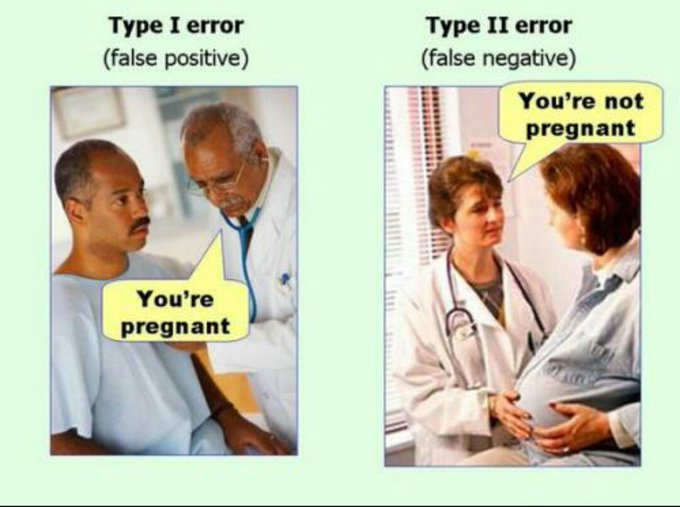
\includegraphics[width=0.85\linewidth]{_images/statisticalErrors} 

}

\caption{The two types of statistical errors}\label{fig:figName72}
\end{figure}

\hypertarget{altre-letture-6}{%
\section{Altre letture}\label{altre-letture-6}}

\begin{enumerate}
\def\labelenumi{\arabic{enumi}.}
\tightlist
\item
  Gigerenzer G (2018) Statistical Rituals: The Replication Delusion and How We Got There. Advances in Methods and Practices in Psychological Science 1(2):198--218, DOI 10.1177/2515245918771329, URL \url{https://journals.sagepub.com/doi/10.1177/2515245918771329}
\end{enumerate}

\hypertarget{esercizi}{%
\section{Esercizi}\label{esercizi}}

\begin{enumerate}
\def\labelenumi{\arabic{enumi}.}
\tightlist
\item
  La nostra miglior stima puntuale del parametro \(\gamma\) di un modello statistico è \(g = -7.2\), con un errore standard pari a 2.8, con 16 gradi di libertà. E'possibile che, in realtà, sia \(\gamma = 0\)? Qual è il P-level per l'ipotesi nulla? Devo accettarla o posso rifiutarla?
\item
  La nostra miglior stima puntuale del parametro \(\delta\) di un modello statistico è \(d = 13.5\), con un errore standard pari a 8.4, ma non è disponibile, per questo errore standard, una stima accurata dei gradi di libertà. E'possibile che, in realtà, sia \(\delta = 0\)? Qual è il P-level per l'ipotesi nulla? Devo accettarla o posso rifiutarla?
\item
  Uno sperimentatore ha impostato un esperimento per confrontare due tesi sperimentali (A, B). I risultati sono i seguenti (in t/ha) \texttt{A\ \textless{}-\ c(9.3,\ 10.2,\ 9.7)} e \texttt{B\ \textless{}-\ c(12.6,\ 12.3,\ 12.5)}. Stabilire se i risultati per le due tesi sperimentali possono essere considerati significativamente diversi, per un livello di probabilità di errore di I specie del 5\%.
\item
  Uno sperimentatore ha impostato un esperimento per confrontare se l'effetto di un fungicida è significativo, in un disegno sperimentale con tre ripetizioni. Con ognuna delle due opzioni di trattamento i livelli di infestazione (in percentuale) sono: \texttt{A\ \textless{}-\ c(6.5,\ 7.1,\ 6.8)} e \texttt{NT\ \textless{}-\ c(54.1,\ 48.2,\ 63.1)}. E'significativo l'effetto del trattamento fungicida, per un livello di probabilità del 5\%? SUGGERIMENTO: prestare attenzione all'omogeneità delle varianze.
\item
  Con un esperimento in laboratorio, abbiamo stimato che il tasso di degradazione di una sostanza xenobiotica in acqua è \(k_1 = -0.071 \pm 0.012\) (7 gradi di libertà). Per una sostanza affine il tasso di degradazione è pari a \(k_2 = -0.153 \pm 0.024\) (7 gradi di lbertà); possiamo concludere che il tasso di degradazione delle due sostanze, in realtà, non è significativamente diverso?
\item
  In un ospedale, è stata misurata la concentrazione di colesterolo nel sangue di otto pazienti, prima e dopo un trattamento medico. Per ogni paziente, sono stati analizzati due campioni, ottenendo le seguenti concentrazioni (in ordine di paziente): \texttt{Prima\ \textless{}-\ c(167.3,\ 186.7,\ 107.0,\ 214.5,\ 149.5,\ 171.5,\ 161.5,\ 243.6)} e \texttt{Dopo\ \textless{}-\ c(166.7,\ 184.2,\ 104.9,\ 205.3,\ 148.5,\ 157.3,\ 149.4,\ 241.5)}. Si può concludere che il trattamento medico è stato efficace?
\item
  Un veterinario ha organizzato un esperimento per valutare l'effetto di una dieta innovativa, sulla pressione arteriosa sistolica di cavalli da corsa. Le informazioni preliminari mostrano con chiarezza che questa dieta innovativa non può avere effetti negativi, ma, eventualmente, solo positivi. Il ricercatore ha selezionato a caso 16 animali, ne ha misurato la pressione arteriosa a riposo ed ha ripetuto la stessa misurazione dopo sei mesi di questa dieta. I risultati ottenuti sono i seguenti: I risultati ottenuti sono: \texttt{prima\ \textless{}-\ c(113.5,\ 116.5,\ 118.1,\ 111.3,\ 116.8,\ 117.0,\ 114.8,\ 114.9,\ 114.8,\ 114.2,\ 115.0,\ 114.0,\ 114.4,\ 116.1,\ 117.9,\ 115.7)} e \texttt{dopo\ \textless{}-\ c(110.9,\ 110.1,\ 110.3,\ 116.8,\ 112.2,\ 111.0,\ 111.1,\ 112.9,\ 110.6,\ 109.1,\ 113.1,\ 109.9,\ 111.9,\ 110.1,\ 114.2,\ 111.0)}. Stabilire se la dieta è efficace, con una probabilità di errore P \textless{} 0.05. SUGGERIMENTO: ricordare che la l'effetto atteso della dieta, per le informazioni preliminari disponibili, può, eventualmente, essere solo quello di abbassare la pressione, mai quello di alzarla.
\item
  I Q.I. di 16 studenti provenienti da un quartiere di una certa città sono risultati pari a: \texttt{QI1\ \textless{}-\ c(90.31,\ 112.63,\ 101.93,\ 121.47,\ 111.37,\ 100.37,\ 106.80,\ 101.57,\ 113.25,\ 120.76,\ \ 88.58,\ 107.53,\ 102.62,\ 104.26,\ 95.06,\ 104.88)}. Gli studenti provenienti da un altro quartiere della stessa città hanno invece mostrato i seguenti Q.I.: \texttt{QI2\ \textless{}-\ c(90.66,\ 101.41,\ 104.61,\ \ 91.77,\ 107.06,\ \ 89.51,\ \ 87.91,\ 92.31,\ 112.96,\ \ 90.33,\ \ 99.86,\ \ 88.99,\ \ 98.97,\ \ 97.92)}. Esiste una differenza significativa tra i Q.I. nei due quartieri della città?
\item
  Viene estratto un campione di rondelle da una macchina in perfette condizioni di funzionamento. Lo spessore delle rondelle misurate è: \texttt{S1\ \textless{}-\ c(0.0451,\ 0.0511,\ 0.0478,\ 0.0477,\ 0.0458,\ 0.0509,\ 0.0446,\ 0.0516,\ 0.0458,\ 0.0490)}. Dopo alcuni giorni, per determinare se la macchina sia ancora a punto, viene estratto un altro campione di 10 rondelle, il cui spessore medio risulta: \texttt{S2\ \textless{}-\ c(0.0502,\ 0.0528,\ 0.0492,\ 0.0556,\ 0.0501,\ 0.0500,\ 0.0498,\ 0.0526,\ 0.0517,\ 0.0550)}. Verificare se la macchina sia ancora ben tarata, oppure necessiti di revisione.
\item
  Le varianze di due campioni composti da 30 unità sono risultate pari, rispettivamente a 115.3 e 356.4; stabilire se il secondo campione ha una varianza significativamente più alta del primo. SUGGERIMENTO: considerare che il rapporto tra due varianze di campioni estratti dalla stessa popolazione gaussiana segue la distribuzione F di Fisher. Considerare anche che, in R, la funzione \texttt{pf(x,\ n1,\ n2,\ lower.tail\ =\ F)} restituisce la probabilità di ottenere valori pari o superiori ad \(x\), da una distribuzione \(F\) di Fisher con \(n1\) ed \(n2\) gradi di libertà. Considerare anche che il rapporto di due varianze può solo essere positivo.
\item
  Un agronomo ha organizzato un esperimento varietale, per confrontare tre varietà di frumento, cioè GUERCINO, ARNOVA e BOLOGNA. Per far questo ha individuato, in un campo uniforme dell'areale umbro, trenta parcelle da 18 m\textsuperscript{2} e ne ha selezionate dieci a caso, da coltivare con GUERCINO, altre dieci a caso sono state coltivate con ARNOVA e le ultime dieci sono state coltivate con BOLOGNA. Al termine dell'esperimento, le produttività osservate erano le seguenti: \texttt{guercino\ \textless{}-\ c(53.2,\ 59.1,\ 62.3,\ 48.6,\ 59.7,\ 60,\ 55.7,\ 55.8,\ 55.7,\ 54.4)}, \texttt{arnova\ \textless{}-\ c(53.1,\ 51,\ 51.9,\ 55.3,\ 58.8,\ 54.6,\ 53,\ 51.4,\ 51.7,\ 64.7)} e \texttt{bologna\ \textless{}-\ c(43.5,\ 41,\ 41.2,\ 44.8,\ 40.2,\ 37.2,\ 45.3,\ 38.9,\ 42.9,\ 39.3)}. Descrivere i tre campioni, utilizzando opportunamente un indicatore di tendenza centrale ed un indicatore di variabilità. Inferire le medie delle tre popolazioni (cioè quelle che hanno generato i tre campioni), utilizzando opportunamente un intervallo di incertezza. Per ognuna delle tre coppie (guercino vs arnova, guercino vs bologna, arnova vs bologna), valutare la differenza tra le medie e il suo errore standard. Valutare la significatività della differenza tra le medie delle tre popolazioni, esplicitando l'ipotesi nulla e calcolando il livello di probabilità di errore nel rifiuto dell'ipotesi nulla.
\end{enumerate}

\hypertarget{verifica-dei-modelli}{%
\chapter{Verifica dei modelli}\label{verifica-dei-modelli}}

Nei capitoli precedenti, abbiamo studiato i modelli come ``strumenti'' per descrivere le relazioni causa-effetto tra le variabili sperimentali e per trarre conclusioni testando ed eventualmente rigettando ipotesi scientifiche rilevanti. Tuttavia, abbiamo anche visto che i modelli statistici e le inferenze su di essi basate, assumono che siano verificate alcune condizioni fondamentali:

\begin{enumerate}
\def\labelenumi{\arabic{enumi}.}
\tightlist
\item
  il modello fornisce una buona descrizione dei dati sperimentali (bontà di adattamento);
\item
  i residui sono indipendenti l'uno dall'altro (indipendenza);
\item
  i residui hanno una distribuzione gaussiana di probabilità (normalità);
\item
  tutti i residui hanno la stessa varianza (omoschedasticità).
\end{enumerate}

Oltre alle ipotesi di cui sopra, i dati osservati devono rispettare anche un altro requisito essenziale: l'assenza di valori anomali (\emph{outliers}), ovvero osservazioni che differiscono notevolmente da tutte le altre osservazioni nello stesso gruppo di trattamento. Questi valori anomali producono residui negativi o positivi enormi, che possono essere molto influenti, sia per il test d'ipotesi che per l'affidabilità delle stime.

Purtroppo, bisogna riconoscere che i problemi relativi alle assunzioni di base sono tutt'altro che infrequenti, come vedremo in seguito.

\hypertarget{deviazioni-rispetto-alle-assunzioni-di-base}{%
\section{Deviazioni rispetto alle assunzioni di base}\label{deviazioni-rispetto-alle-assunzioni-di-base}}

La mancanza di `bontà d'adattamento' (più semplicemente: `mancanza d'adattamento') può verificarsi quando le previsioni del modello sembrano deviare sistematicamente rispetto ai dati osservati, ad esempio quando una modello di regressione lineare viene adattato ad una risposta curvilinea. In caso di mancanza di adattamento, dovremo concludere che i dati e il modello non si supportano a vicenda e, quindi, che il modello ``non consente al ricercatore di rispondere alle sue domande scientifiche'' (Kass et al., 2016).

La mancanza d'indipendenza dei residui del modello può verificarsi a causa di:

\begin{enumerate}
\def\labelenumi{\arabic{enumi}.}
\tightlist
\item
  intrusioni sistematiche,
\item
  presenza di fattori di raggruppamento non considerati nel modello,
\item
  mancanza di adattamento sistematica dovuta alla selezione errata del modello, o
\item
  mancanza di randomizzazione adeguata (vedere anche Sezione 4.6 e Capitolo 12).
\end{enumerate}

La mancanza di indipendenza è considerata una delle assunzioni di base più pericolose da violare, poiché comporta un rischio elevato di errore di I specie (Frey et al., 2024), ovvero un rischio maggiore di rifiutare erroneamente un'ipotesi nulla vera (falso positivo).

La normalità viene violata quando i residui del modello non ``riflettono'' la forma tipica di una distribuzione gaussiana, ovvero quando sono asimmetrici (distribuzione asimmetrica: la media non è uguale alla mediana) o quando le code sono troppo `alte' (distribuzione platicurtica: troppi valori estremi) o troppo `basse' (distribuzione leptocurtica: i valori sono troppo ``concentrati'' attorno alla media)(Fig. \ref{fig:figName100prima}). In assenza di \emph{outliers} (vedi più avanti), la non normalità è considerata meno dannosa di altre deviazioni (Knief e Forstmeier, 2021), in quanto non provoca forti distorsioni nella stima dei parametri od un incremento del rischio di errore di I specie. Tuttavia, si raccomanda sempre un atteggiamento cauto, poiché le deviazioni dalla normalità possono essere associate ad altri tipi di deviazioni più pericolose, come l'eteroschedasticità. Deviazioni dalla normalità possono verificarsi anche a causa della presenza di \emph{outliers}, collegati ad errori casuali di entità eccezionale (ad esempio, procedure difettose, scarso controllo o intrusioni di qualsiasi tipo). Questi \emph{outliers} modificano profondamente medie e deviazioni standard, portando ad un'errata interpretazione dei risultati sperimentali (Cochran, 1947).

\begin{figure}

{\centering 
\includegraphics[width=0.85\linewidth]{_main_files/figure-latex/figName100prima-1} 

}

\caption{Alcune distribuzioni non-normali dei residui.}\label{fig:figName100prima}
\end{figure}

L'eteroschedasticità può verificarsi, ad esempio, quando i trattamenti sperimentali producono effetti sia sulla media che sulle deviazioni standard (ad esempio, effetti moltiplicativi) in modo tale che queste due statistiche diventino proporzionali tra loro (quando la media aumenta, aumenta proporzionalmente anche la deviazione standard). Altre cause comuni di eteroschedasticità includono attacchi di parassiti e altre intrusioni, nonché un grado inferiore di controllo in alcune parti dell'esperimento di campo. È stato dimostrato che l'eteroschedasticità si traduce in una stima distorta della deviazione standard dei residui e porta a P-value non validi, così che il reale rischio d'errore di I specie può essere anche molto diverso da quello nominale (Glass et al., 1972).

\hypertarget{scoprire-le-violazioni}{%
\section{Scoprire le violazioni}\label{scoprire-le-violazioni}}

Il rispetto di alcune assunzioni di base, come l'indipendenza dei residui e l'assenza di errori sistematici, è garantito dall'adozione di un disegno sperimentale a `regola d'arte', cioè basato su repliche indipendenti e correttamente randomizzate. Bisogna tenere presente che gli eventuali vincoli alla randomizzazione introdotti in fase di disegno sperimentale (blocchi randomizzati, quadrato latino, split-plot\ldots) possono inficiare l'indipendenza dei residui; ad esempio, con i blocchi randomizzati, le osservazioni all'interno dello stesso blocco si assomigliano di più che non quelle in blocchi diversi, proprio perché condividono le condizioni ambientali caratteristiche di ciascun blocco. Insomma, si realizza un certo grado di `parentela' tra le osservazioni, che non è compatibile con l'ipotesi di totale indipendenza. Vedremo nei capitoli successivi che queste situazioni vengono gestite includendo nel modello ANOVA anche il fattore di blocco o gli altri vincoli eventualmente imposti alla randomizzazione completa.

Per quanto riguarda le altre assunzioni di base, come la bontà di adattamento, l'omogeneità delle varianze e la normalità dei residui, la verifica può essere fatta solo \emph{a posteriori}, cioè dopo aver effettuato la stima dei parametri ed aver individuato i residui stessi.

Oltre a quanto abbiamo finora dotto, dobbiamo anche tener presente che il dataset non dovrebbe contenere le cosiddette osservazioni aberranti od \emph{outliers}. Si tratta di osservazioni molto diverse dalle altre, che spesso fanno sospettare che sia avvenuto qualche errore grossolano; la loro assenza non è postulata da alcun modello statistico, anche se esse, proprio perché molto diverse dalle altre, finiscono per inficiare la normalità dei residui e l'omogeneità delle varianze, oltre a stravolgere pericolosamente le nostre conclusioni. Pertanto, alla loro individuazione deve essere sempre dedicata la debita attenzione.

Per diagnosticare eventuali problemi con le assunzioni di base e/o con la presenza di outliers, possiamo utilizzare sia metodi grafici che metodi formali, basati sul test d'ipotesi. Vediamo ora alcune possibilità.

\hypertarget{analisi-grafica-dei-residui}{%
\section{Analisi grafica dei residui}\label{analisi-grafica-dei-residui}}

Dato che la gran parte delle assunzioni riguarda la struttura dei residui, l'ispezione grafica di questi ultimi è in grado di evidenziare chiaramente la gran parte dei problemi e dovrebbe, pertanto, essere considerata come una metodica da applicare in modo routinario. Esistono diversi tipi di grafici, ma ne elenchiamo fondamentalmente due: il grafico dei residui contro i valori attesi e il QQ-plot.

\hypertarget{grafico-dei-valori-osservati-aumentato-con-le-previsioni-del-modello}{%
\subsection{Grafico dei valori osservati, aumentato con le previsioni del modello}\label{grafico-dei-valori-osservati-aumentato-con-le-previsioni-del-modello}}

Per tutti i tipi di modelli di regressione, lo strumento più importante per verificare la bontà di adattamento è un grafico a dispersione della risposta osservata rispetto al predittore, integQuest'ultima dovrebbe seguire fedelmente i dati osservati (Fig. \ref{fig:figName100}A) senza mostrare alcun segno di deviazioni sistematiche, come illustrato nelle Figure \ref{fig:figName100}B, C e D.

\begin{figure}

{\centering 
\includegraphics{_main_files/figure-latex/figName100-1} 

}

\caption{Grafico a dispersione delle risposte osservate (simboli), integrati con le previsioni del modello (linee e curve). Il panel in alto a sinistra mostra un modello con un buon adattamento, mentre gli altri grafici mostrano diversi tipi di violazioni.}\label{fig:figName100}
\end{figure}

\hypertarget{grafico-dei-residui-contro-i-valori-attesi}{%
\subsection{Grafico dei residui contro i valori attesi}\label{grafico-dei-residui-contro-i-valori-attesi}}

Il metodo grafico più utilizzato per l'analisi dei residui consiste nel plottare i residui stessi contro i valori attesi. Se non vi sono problemi, i punti nel grafico dovrebbero essere distribuiti in modo assolutamente casuale, come in Figura \ref{fig:figName101}, in alto a sinistra. Le osservazioni aberranti (\emph{outliers}) appaiono invece come punti isolati rispetto agli altri (Fig. \ref{fig:figName101}; in alto a destra). L'eterogeneità delle varianze è invece indicata da residui che si allargano o si stringono procedendo verso i margini del grafico (Figura \ref{fig:figName101}, in basso a sinistra), facendo emergere una sorta di proporzionalità tra media e varianza. In ultimo, la mancanza di adattamento nei modelli di regressione è evidenziata da un qualche evidente \emph{pattern}, come quando i residui sono tendenzialmente negativi per bassi valori attesi e positivi per alti valori, chiaro segnale di un modello deterministico che sovrastima le osservazioni quando sono basse e le sottostima quando sono alte (Fig. \ref{fig:figName101}; in basso a destra).

\begin{figure}

{\centering 
\includegraphics{_main_files/figure-latex/figName101-1} 

}

\caption{Plot dei residui contro i valori attesi: una disposizione dei punti totalmente casuale supportata l'ipotesi che le assunzioni di base siano rispettate (in alto a sinistra). Gli *outliers* sono evidenziati come punti 'isolati' (in alto a destra), mentre una disposizione ad 'imbuto' rivela che le varianze sono direttamente o inversamente proporzionali alle medie (in basso a sinistra). La mancanza d'adattamento è invece rivelata da un qualkunque evidente pattern nella disposizione dei punti, come, ad esempio, dei residui associati di ugual segno in una certa zona del grafico (in basso a destra).}\label{fig:figName101}
\end{figure}

\hypertarget{qq-plot}{%
\subsection{QQ-plot}\label{qq-plot}}

Per evidenziare problemi di non-normalità, risulta molto utile un QQ-plot (quantile-quantile plot), nel quale i residui \emph{standardizzati} vengono `plottati' contro i rispettivi percentili di una distribuzione normale standardizzata. Con residui normali, queste due entità (i residui standardizzati e i percentili corrispondenti di una distribuzione normale standardizzata) sono largamente coincidenti, in modo che i punti nel QQ-plot giacciono lungo la bisettrice del primo e del terzo quadrante (\ref{fig:figName105} in alto a sinistra).

Le deviazioni più diffuse dalla normalità sono relative alla simmetria (skewness) e alla curtosi della popolazione da cui i residui sono campionati. In particolare, può capitare che i residui provengano da una popolazione con asimmetria positiva (right-skewed), come, ad esempio, una popolazione log-normale. In questo caso, la media è maggiore della mediana e i residui negativi sono più numerosi, ma più piccoli in valore assoluto di quelli positivi. Il QQ-plot si presenta come in figura \ref{fig:figName105} in alto al centro. Al contrario, se i residui provengono da una popolazione con asimmetria negativa (`left-skewed'), caratterizzata, ad esempio, da una funzione di densità `beta', la media è minore della mediana e, di conseguenza, i valori positivi sono più numerosi, ma più vicini allo zero di quelli negativi. In questa situazione, il QQ-plot presenta un andamento abbastanza tipico, come indicato in Figura \ref{fig:figName105} in alto a destra.

Per quanto riguarda la curtosi, è necessario osservare le code della distribuzione: se queste sono più alte di una distribuzione normale parliamo di distribuzione platicurtica, mentre se sono più basse parliamo di distribuzione leptocurtica. Ad esempio, se i residui provengono da una distribuzione t di Student con pochi gradi di libertà sono platicurtici ed il QQ-plot mostra l'andamento indicato in figura \ref{fig:figName105} in basso a sinistra. Al contrario, se i residui provengono da una distribuzione uniforme sono tipicamente leptocurtici e presentano un QQ-plot come quello riportato in Figura \ref{fig:figName105} in basso al centro.

\begin{figure}

{\centering 
\includegraphics{_main_files/figure-latex/figName105-1} 

}

\caption{QQ-plot per residui gaussiani (in alto a sinistra) e per residui che mostrano diversi tipi di violazioni dalla normalità (vedi anche Fig. 8.1).}\label{fig:figName105}
\end{figure}

\hypertarget{test-dipotesi}{%
\section{Test d'ipotesi}\label{test-dipotesi}}

La valutazioni illustrate in precedenza sono basate sulla semplice osservazione di uno o più grafici, ma sono considerate sufficientemente attendibili per la maggior parte delle situazioni. Tuttavia, esistono anche test statistici formali che consentono di saggiare l'ipotesi nulla di `assenza di deviazioni', che può essere rifiutata qualora il P-level fosse inferiore a 0.05.

Rispetto alle procedure grafiche, il test d'ipotesi formale può dare una miglior sensazione di obiettività, anche se non è tutto oro quel che luccica. Infatti, questi test possono creare più problemi di quanti ne risolvano dato che, ad esempio, richiedono campioni di grandi dimensioni e fanno affidamento su assunzioni di base molto stringenti, tanto che, alla fine, l'affidabilità dei risultati è spesso discutibile (Kozak e Piepho 2018). Per questi motivi, il loro utilizzo è sconsigliato e dovrebbe essere riservato a supportare situazioni complesse in cui i metodi grafici non forniscono risposte sufficientemente chiare.

Le procedure presentate in questo capitolo sono state selezionate perché ampiamente utilizzate e facilmente disponibili in R.

\hypertarget{test-di-levene-per-lomogeneituxe0-delle-varianze}{%
\subsection{Test di Levene per l'omogeneità delle varianze}\label{test-di-levene-per-lomogeneituxe0-delle-varianze}}

Secondo gli studi di Conover et al.~(1981), il test di Levene è una delle procedure più affidabili per saggiare l'ipotesi di omoschedasticità nei modelli con predittori nominali; consiste nel'eseguire l'analisi della varianza di una `pseudo-risposta', ottenuta sostituendo ciascun dato osservato con il valore assoluto della sua differenza con il centro del gruppo a cui appartiene (dati `group-centered').

Inizialmente, Levene propose di utilizzare come centro di gruppo la media; l'idea di fondo era che, sebbene le medie di gruppo di dati `group-centered' siano pari a zero, prendendo i valori assoluto (cioè rimuovendo i segno negativi), queste medie diventano diverse da zero e sono tanto più alte quanto più la varianza di gruppo è alta. Questo concetto sarà più semplice da comprendere utilizzando un esempio pratico. Consideriamo due gruppi sperimentali \texttt{A\ \textless{}-\ c(19,\ 20,\ 21)} e \texttt{B\ \textless{}-\ c(26,\ 30,\ 34)}, che hanno, rispettivamente, medie pari a 20 e 30, e varianze pari a 1 e 16. Sottraendo dalle osservazioni di ogni gruppo la media del gruppo stesso, otteniamo le pseudo-osservazioni \texttt{Ac\ \textless{}-\ c(-1,\ 0,\ 1)} e \texttt{Bc\ \textless{}-\ c(-4,\ 0,\ 4)}, la cui media è zero, mentre le varianze restano inalterate. Se escludiamo i segno negativi, le medie dei due gruppi divengono pari, rispettivamente, a 2/3 e 8/3, mostrando come il gruppo con più alta varianza abbia prodotto pseudo-osservazioni con media più alta. Se la differenza tra le due medie delle pseudo-osservazioni è significativa, l'ipotesi nulla di omogeneità delle varianze può essere rigettata.

Lavori successivi (Brown e Forsythe, 1974) hanno mostrato che è preferibile sostituire la media del gruppo con la sua mediana, per ottenere un test più robusto per dati non normali.

Sia il test di Levene che il test di Brown-Forsythe sono disponibili nella funzione \texttt{leveneTest()} del package \texttt{car}, ma il secondo è largamente preferito e considerato come la procedura di `default'. Un esempio di questo test è fornito nel Riquadro 8.3, che confronta due genotipi di mais in un disegno completamente randomizzato con 11 repliche. Il secondo genotipo (B) presenta una varianza maggiore e il test di Levene risulta significativo (il valore P è inferiore a 0,05 e l'ipotesi nulla di omoschedasticità viene rifiutata). I due test (centrato sulle medie o centrato sulle mediane) producono risultati simili, il che potrebbe suggerire che i dati originali non si discostino significativamente dalla normalità.

\begin{Shaded}
\begin{Highlighting}[]
\CommentTok{\# Code Box 8.1}
\CommentTok{\# Testing hypotheses about model residuals}
\CommentTok{\# Levene’s test for homoscedasticity}
\FunctionTok{library}\NormalTok{(car)}

\CommentTok{\# Entering the data}
\NormalTok{dataset }\OtherTok{\textless{}{-}} \FunctionTok{data.frame}\NormalTok{(}\AttributeTok{Genotype =} \FunctionTok{c}\NormalTok{(}\StringTok{"A"}\NormalTok{, }\StringTok{"A"}\NormalTok{, }\StringTok{"A"}\NormalTok{, }\StringTok{"A"}\NormalTok{, }\StringTok{"A"}\NormalTok{,}
                                   \StringTok{"A"}\NormalTok{, }\StringTok{"A"}\NormalTok{, }\StringTok{"A"}\NormalTok{, }\StringTok{"A"}\NormalTok{, }\StringTok{"A"}\NormalTok{,}
                                   \StringTok{"A"}\NormalTok{, }\StringTok{"B"}\NormalTok{, }\StringTok{"B"}\NormalTok{, }\StringTok{"B"}\NormalTok{, }\StringTok{"B"}\NormalTok{,}
                                   \StringTok{"B"}\NormalTok{, }\StringTok{"B"}\NormalTok{, }\StringTok{"B"}\NormalTok{, }\StringTok{"B"}\NormalTok{, }\StringTok{"B"}\NormalTok{,}
                                   \StringTok{"B"}\NormalTok{, }\StringTok{"B"}\NormalTok{),}
                      \AttributeTok{Yield =} \FunctionTok{c}\NormalTok{(}\FloatTok{10.0}\NormalTok{, }\FloatTok{10.7}\NormalTok{, }\FloatTok{11.9}\NormalTok{, }\FloatTok{10.3}\NormalTok{, }\FloatTok{10.0}\NormalTok{,}
                                \FloatTok{7.8}\NormalTok{, }\FloatTok{10.4}\NormalTok{, }\FloatTok{9.7}\NormalTok{, }\FloatTok{10.0}\NormalTok{, }\FloatTok{9.2}\NormalTok{, }\FloatTok{9.7}\NormalTok{,}
                                \FloatTok{15.0}\NormalTok{, }\FloatTok{11.2}\NormalTok{, }\FloatTok{13.7}\NormalTok{, }\FloatTok{11.9}\NormalTok{, }\FloatTok{9.4}\NormalTok{,}
                                \FloatTok{10.6}\NormalTok{, }\FloatTok{12.6}\NormalTok{, }\FloatTok{10.1}\NormalTok{, }\FloatTok{9.9}\NormalTok{, }\FloatTok{15.3}\NormalTok{, }\FloatTok{12.2}\NormalTok{))}
\FunctionTok{head}\NormalTok{(dataset)}
\DocumentationTok{\#\#   Genotype Yield}
\DocumentationTok{\#\# 1        A  10.0}
\DocumentationTok{\#\# 2        A  10.7}
\DocumentationTok{\#\# 3        A  11.9}
\DocumentationTok{\#\# 4        A  10.3}
\DocumentationTok{\#\# 5        A  10.0}
\DocumentationTok{\#\# 6        A   7.8}
\NormalTok{dataset}\SpecialCharTok{$}\NormalTok{Genotype }\OtherTok{\textless{}{-}} \FunctionTok{factor}\NormalTok{(dataset}\SpecialCharTok{$}\NormalTok{Genotype)}

\CommentTok{\# Fitting the model}
\NormalTok{mod }\OtherTok{\textless{}{-}} \FunctionTok{lm}\NormalTok{(Yield }\SpecialCharTok{\textasciitilde{}}\NormalTok{ Genotype, }\AttributeTok{data =}\NormalTok{ dataset)}

\CommentTok{\# Centering the data by subtracting, for each genotype }
\CommentTok{\# the group mean (Levene’s test)}
\NormalTok{GroupMeans }\OtherTok{\textless{}{-}} \FunctionTok{tapply}\NormalTok{(dataset}\SpecialCharTok{$}\NormalTok{Yield, dataset}\SpecialCharTok{$}\NormalTok{Genotype, mean)}
\NormalTok{YieldC }\OtherTok{\textless{}{-}}\NormalTok{ dataset}\SpecialCharTok{$}\NormalTok{Yield }\SpecialCharTok{{-}} \FunctionTok{rep}\NormalTok{(GroupMeans, }\AttributeTok{each =} \DecValTok{11}\NormalTok{)}

\CommentTok{\# Re{-}fitting the same model to the absolute values of }
\CommentTok{\# centered data and run an ANOVA}
\NormalTok{modlevene }\OtherTok{\textless{}{-}} \FunctionTok{lm}\NormalTok{(}\FunctionTok{abs}\NormalTok{(YieldC) }\SpecialCharTok{\textasciitilde{}}\NormalTok{ dataset}\SpecialCharTok{$}\NormalTok{Genotype)}
\FunctionTok{anova}\NormalTok{(modlevene)}
\DocumentationTok{\#\# Analysis of Variance Table}
\DocumentationTok{\#\# }
\DocumentationTok{\#\# Response: abs(YieldC)}
\DocumentationTok{\#\#                  Df  Sum Sq Mean Sq F value  Pr(\textgreater{}F)  }
\DocumentationTok{\#\# dataset$Genotype  1  5.2129  5.2129  5.8944 0.02475 *}
\DocumentationTok{\#\# Residuals        20 17.6878  0.8844                  }
\DocumentationTok{\#\# {-}{-}{-}}
\DocumentationTok{\#\# Signif. codes:  0 \textquotesingle{}***\textquotesingle{} 0.001 \textquotesingle{}**\textquotesingle{} 0.01 \textquotesingle{}*\textquotesingle{} 0.05 \textquotesingle{}.\textquotesingle{} 0.1 \textquotesingle{} \textquotesingle{} 1}
\CommentTok{\# Centering the data by subtracting, for each genotype}
\CommentTok{\# the group median (Brown{-}Forsythe’s test)}
\NormalTok{GroupMedians }\OtherTok{\textless{}{-}} \FunctionTok{tapply}\NormalTok{(dataset}\SpecialCharTok{$}\NormalTok{Yield, dataset}\SpecialCharTok{$}\NormalTok{Genotype, median)}
\NormalTok{YieldC }\OtherTok{\textless{}{-}}\NormalTok{ dataset}\SpecialCharTok{$}\NormalTok{Yield }\SpecialCharTok{{-}} \FunctionTok{rep}\NormalTok{(GroupMedians, }\AttributeTok{each =} \DecValTok{11}\NormalTok{)}

\CommentTok{\# Re{-}fitting the same model to the absolute values of \# centered data and run an ANOVA}
\NormalTok{modlevene }\OtherTok{\textless{}{-}} \FunctionTok{lm}\NormalTok{(}\FunctionTok{abs}\NormalTok{(YieldC) }\SpecialCharTok{\textasciitilde{}}\NormalTok{ dataset}\SpecialCharTok{$}\NormalTok{Genotype)}
\FunctionTok{anova}\NormalTok{(modlevene)}
\DocumentationTok{\#\# Analysis of Variance Table}
\DocumentationTok{\#\# }
\DocumentationTok{\#\# Response: abs(YieldC)}
\DocumentationTok{\#\#                  Df  Sum Sq Mean Sq F value  Pr(\textgreater{}F)  }
\DocumentationTok{\#\# dataset$Genotype  1  5.2041  5.2041  5.7245 0.02666 *}
\DocumentationTok{\#\# Residuals        20 18.1818  0.9091                  }
\DocumentationTok{\#\# {-}{-}{-}}
\DocumentationTok{\#\# Signif. codes:  0 \textquotesingle{}***\textquotesingle{} 0.001 \textquotesingle{}**\textquotesingle{} 0.01 \textquotesingle{}*\textquotesingle{} 0.05 \textquotesingle{}.\textquotesingle{} 0.1 \textquotesingle{} \textquotesingle{} 1}
\CommentTok{\# Non{-}robust Levene’s test with R (centering with means)}
\FunctionTok{leveneTest}\NormalTok{(mod, }\AttributeTok{center =} \StringTok{"mean"}\NormalTok{)}
\DocumentationTok{\#\# Levene\textquotesingle{}s Test for Homogeneity of Variance (center = "mean")}
\DocumentationTok{\#\#       Df F value  Pr(\textgreater{}F)  }
\DocumentationTok{\#\# group  1  5.8944 0.02475 *}
\DocumentationTok{\#\#       20                  }
\DocumentationTok{\#\# {-}{-}{-}}
\DocumentationTok{\#\# Signif. codes:  0 \textquotesingle{}***\textquotesingle{} 0.001 \textquotesingle{}**\textquotesingle{} 0.01 \textquotesingle{}*\textquotesingle{} 0.05 \textquotesingle{}.\textquotesingle{} 0.1 \textquotesingle{} \textquotesingle{} 1}
\CommentTok{\# Levene’s test with R (centering with medians; default)}
\FunctionTok{leveneTest}\NormalTok{(mod)}
\DocumentationTok{\#\# Levene\textquotesingle{}s Test for Homogeneity of Variance (center = median)}
\DocumentationTok{\#\#       Df F value  Pr(\textgreater{}F)  }
\DocumentationTok{\#\# group  1  5.7245 0.02666 *}
\DocumentationTok{\#\#       20                  }
\DocumentationTok{\#\# {-}{-}{-}}
\DocumentationTok{\#\# Signif. codes:  0 \textquotesingle{}***\textquotesingle{} 0.001 \textquotesingle{}**\textquotesingle{} 0.01 \textquotesingle{}*\textquotesingle{} 0.05 \textquotesingle{}.\textquotesingle{} 0.1 \textquotesingle{} \textquotesingle{} 1}
\end{Highlighting}
\end{Shaded}

\hypertarget{test-di-shapiro-wilk-per-la-normalituxe0}{%
\subsection{Test di Shapiro-Wilk per la normalità}\label{test-di-shapiro-wilk-per-la-normalituxe0}}

Il test di Shapiro-Wilk per la normalità fornisce la statistica W e un valore P per l'ipotesi nulla che i residui siano distribuiti normalmente. La procedura di test non è così semplice come quella del test di Levene e i calcoli manuali non sono altrettanto facili da eseguire. Tuttavia, possiamo utilizzare la funzione \texttt{shapiro.test()} in R, passando i residui del modello come argomento (vedi l'esempio seguente).

\hypertarget{altri-test}{%
\subsection{Altri test}\label{altri-test}}

Vale la pena menzionare alcune tecniche numeriche per l'individuazione di valori anomali, come i metodi proposti da Anscombe e Tukey (1963) e Grubbs (1969).

\hypertarget{esempio-8.1-analisi-dei-residui-per-il-dataset-mixture}{%
\section{Esempio 8.1: Analisi dei residui per il dataset ``mixture''}\label{esempio-8.1-analisi-dei-residui-per-il-dataset-mixture}}

Abbiamo eseguito un esperimento in vaso, nel quale abbiamo utilizzato quattro trattamenti erbicidi:

\begin{enumerate}
\def\labelenumi{\arabic{enumi}.}
\tightlist
\item
  Metribuzin
\item
  Rimsulfuron
\item
  Metribuzin + rimsulfuron
\item
  Testimone non trattato
\end{enumerate}

Lo scopo dell'esperimento era quello di verificare se la miscela metribuzin e rimsulfuron è più efficace dei due componenti utilizzati separatamente.

A questo fine, sono stati preparati sedici vasi uniformi e sono stati seminati con \emph{Solanum nigrum}, un importante infestante di alcune colture primaverili estive, come mais e pomodoro. Quando le piante hanno raggiunto lo stadio di 4 foglie vere, sono state trattate con una delle tesi sopra elencate, secondo un disegno sperimentale completamente randomizzato con quattro repliche. Tre settimane dopo i trattamenti, le piante in ciascun vaso sono state raccolte e pesate; minore era il peso, maggiore era l'efficacia degli erbicidi (Onofri et al.~1995).

Per questo esperimento, è possibile adattare un modello lineare con un predittore nominale (il trattamento erbicida) (vedere Eq. 4.6 nel Cap. 4), come mostrato nel riquadro sottostante.

\begin{Shaded}
\begin{Highlighting}[]
\CommentTok{\# Code box 8.2}
\CommentTok{\# Example 8.1}
\CommentTok{\# Checking the residuals for the \textasciigrave{}mixture\textquotesingle{} data}

\CommentTok{\# Loading the packages}
\FunctionTok{library}\NormalTok{(statforbiology)}
\FunctionTok{library}\NormalTok{(car)}

\CommentTok{\# Loading and transforming the data}
\NormalTok{mixture }\OtherTok{\textless{}{-}} \FunctionTok{getAgroData}\NormalTok{(}\StringTok{"mixture"}\NormalTok{)}
\NormalTok{mixture}\SpecialCharTok{$}\NormalTok{Treat }\OtherTok{\textless{}{-}} \FunctionTok{factor}\NormalTok{(mixture}\SpecialCharTok{$}\NormalTok{Treat)}
\FunctionTok{head}\NormalTok{(mixture)}
\DocumentationTok{\#\#             Treat Weight}
\DocumentationTok{\#\# 1 Metribuzin\_\_348  15.20}
\DocumentationTok{\#\# 2 Metribuzin\_\_348   4.38}
\DocumentationTok{\#\# 3 Metribuzin\_\_348  10.32}
\DocumentationTok{\#\# 4 Metribuzin\_\_348   6.80}
\DocumentationTok{\#\# 5     Mixture\_378   6.14}
\DocumentationTok{\#\# 6     Mixture\_378   1.95}
\CommentTok{\# Model fitting}
\NormalTok{mod1 }\OtherTok{\textless{}{-}} \FunctionTok{lm}\NormalTok{(Weight }\SpecialCharTok{\textasciitilde{}}\NormalTok{ Treat, }\AttributeTok{data =}\NormalTok{ mixture)}
\end{Highlighting}
\end{Shaded}

Dopo aver effettuato la stima dei parametri, i grafici dei residui possono essere ottenuti utilizzando la funzione \texttt{plot()} applicata al risultato del fitting lineare. L'argomento `which' specifica il tipo di grafico: se utilizziamo: `which = 1' otteniamo il grafico dei residui verso gli attesi, se invece utilizziamo `which = 2' otteniamo il QQ-plot. I due comandi sono:

\begin{verbatim}
plot(mod, which = 1)
plot(mod, which = 2)
\end{verbatim}

e il risultato è mostrato nella figura \ref{fig:figName110a}.

\begin{figure}

{\centering 
\includegraphics[width=0.85\linewidth]{_main_files/figure-latex/figName110a-1} 

}

\caption{Analisi grafica dei residui per un modello ANOVA ad una via adattato al dataset 'mixture.csv'}\label{fig:figName110a}
\end{figure}

Nessuno dei grafici suggerisce l'esistenza di particolari problematiche e, considerando anche che che non si tratta di un conteggio o una proporzione e che le differenze tra le medie sono piuttosto piccole (meno di un ordine di grandezza), possiamo concludere che non vi sono motivi per dubitare del rispetto delle assunzioni di base.

Sebbene ciò non sia necessario, possiamo confermare la nostra conclusione eseguendo i test di Levene e Shapiro-Wilk. Nel codice sottostante possiamo notare come la funzione \texttt{leveneTest()} richieda come argomento l'oggetto risultante dal fitting lineare, mentre la funzione \texttt{shapiro.test()} richiede i residui del modello.

\begin{Shaded}
\begin{Highlighting}[]
\CommentTok{\# Example 8.1 [continuation]}

\CommentTok{\# Levene\textquotesingle{}s test and Shapiro{-}Wilk\textquotesingle{}s test}
\FunctionTok{leveneTest}\NormalTok{(mod1)}
\DocumentationTok{\#\# Levene\textquotesingle{}s Test for Homogeneity of Variance (center = median)}
\DocumentationTok{\#\#       Df F value Pr(\textgreater{}F)}
\DocumentationTok{\#\# group  3  1.0698 0.3984}
\DocumentationTok{\#\#       12}
\FunctionTok{shapiro.test}\NormalTok{(}\FunctionTok{residuals}\NormalTok{(mod1))}
\DocumentationTok{\#\# }
\DocumentationTok{\#\#  Shapiro{-}Wilk normality test}
\DocumentationTok{\#\# }
\DocumentationTok{\#\# data:  residuals(mod1)}
\DocumentationTok{\#\# W = 0.97615, p{-}value = 0.9257}
\end{Highlighting}
\end{Shaded}

\hypertarget{esempio-8.2-analisi-dei-residui-per-il-dataset-insects}{%
\section{Esempio 8.2: Analisi dei residui per il dataset `insects'}\label{esempio-8.2-analisi-dei-residui-per-il-dataset-insects}}

Proviamo ad analizzare il dataset `insects', che si riferisce ad un esperimento nel quale quindici piante sono state trattate con tre insetticidi diversi in modo completamente randomizzato, scegliendo cinque piante a caso per insetticida. Tre settimane dopo il trattamento è stato rilevato il numero di insetti presenti su ciascuna pianta.

Per testare l'effetto degli insetticidi, è stato adattato ai dati osservati un modello ANOVA ad una via, utilizzando la variabile ``Insecticide'' come predittore nominale. In questo caso, il controllo delle deviazioni dagli assunti di base richiede grande attenzione, poiché la variabile di risposta è un conteggio e le statistiche descrittive, che si lasciano per eercizio al lettore, indicano che le deviazioni standard sono in qualche modo proporzionali alle medie. Le analisi grafiche dei residui in Figura \ref{fig:figName110} mostrano chiari segni di eteroschedasticità (grafico a sinistra) e residui asimmetrici a destra (grafico a destra). Queste deviazioni sono confermate dal test di Levene (valore P = 0,043) e dal test di Shapiro-Wilks (valore P = 0,048).

\begin{Shaded}
\begin{Highlighting}[]
\CommentTok{\# Example 8.2}
\CommentTok{\# checking the residuals for the \textasciigrave{}insects\textquotesingle{} data}

\CommentTok{\# Loading the packages}
\FunctionTok{library}\NormalTok{(statforbiology)}
\FunctionTok{library}\NormalTok{(car)}

\CommentTok{\# Loading and transforming the data}
\NormalTok{insects }\OtherTok{\textless{}{-}} \FunctionTok{getAgroData}\NormalTok{(}\StringTok{"insects"}\NormalTok{)}
\NormalTok{insects}\SpecialCharTok{$}\NormalTok{Insecticide }\OtherTok{\textless{}{-}} \FunctionTok{factor}\NormalTok{(insects}\SpecialCharTok{$}\NormalTok{Insecticide)}
\FunctionTok{head}\NormalTok{(insects)}
\DocumentationTok{\#\#   Insecticide Rep Count}
\DocumentationTok{\#\# 1          T1   1   448}
\DocumentationTok{\#\# 2          T1   2   906}
\DocumentationTok{\#\# 3          T1   3   484}
\DocumentationTok{\#\# 4          T1   4   477}
\DocumentationTok{\#\# 5          T1   5   634}
\DocumentationTok{\#\# 6          T2   1   211}
\CommentTok{\# Fitting a model}
\NormalTok{mod2 }\OtherTok{\textless{}{-}} \FunctionTok{lm}\NormalTok{(Count }\SpecialCharTok{\textasciitilde{}}\NormalTok{ Insecticide, }\AttributeTok{data =}\NormalTok{ insects)}

\CommentTok{\# Graphical analyses of residuals (not run, see Figure)}
\CommentTok{\# plot(mod2, which = 1)}
\CommentTok{\# plot(mod2, which = 2)}

\CommentTok{\# Levene\textquotesingle{}s test}
\FunctionTok{leveneTest}\NormalTok{(mod2)}
\DocumentationTok{\#\# Levene\textquotesingle{}s Test for Homogeneity of Variance (center = median)}
\DocumentationTok{\#\#       Df F value Pr(\textgreater{}F)}
\DocumentationTok{\#\# group  2  1.0263 0.3878}
\DocumentationTok{\#\#       12}
\CommentTok{\# Shapiro{-}Wilks\textquotesingle{} test}
\FunctionTok{shapiro.test}\NormalTok{(}\FunctionTok{residuals}\NormalTok{(mod2))}
\DocumentationTok{\#\# }
\DocumentationTok{\#\#  Shapiro{-}Wilk normality test}
\DocumentationTok{\#\# }
\DocumentationTok{\#\# data:  residuals(mod2)}
\DocumentationTok{\#\# W = 0.87689, p{-}value = 0.04265}
\end{Highlighting}
\end{Shaded}

\begin{figure}

{\centering 
\includegraphics[width=0.85\linewidth]{_main_files/figure-latex/figName110-1} 

}

\caption{Analisi grafica dei residui per il dataset 'insects.csv'}\label{fig:figName110}
\end{figure}

\hypertarget{misure-correttive}{%
\section{Misure correttive}\label{misure-correttive}}

Se le procedure diagnostiche hanno evidenziato deviazioni rispetto agli assunti di base, è necessario valutare se e come intraprendere azioni correttive. Ovviamente, la `terapia' cambia al cambiare della `patologia'.

\hypertarget{correzionerimozione-degli-outliers}{%
\subsection{Correzione/Rimozione degli outliers}\label{correzionerimozione-degli-outliers}}

In presenza di outliers, la `terapia' più opportuna è, banalmente, quella di rimuoverli, ottenendo così un dataset `sbilanciato' (diverso numero di repliche per trattamento). Oggigiorno, trattare un dataset sbilanciato non costituisce un problema, ovviamente se si utilizzano le metodiche di analisi opportune. Qualche anno fa, al contrario, si cercava di evitare lo sbilanciamento a tutti i costi, utilizzando tecniche di \emph{imputing} per l'immissione di valori `ragionevoli' in sostituzione di quelli mancanti/aberranti. Con le dovute eccezioni, le tecniche di \emph{imputing} sembrano oggi abbastanza obsolete, almeno in questo contesto.

Vorremmo porre l'attenzione sul fatto che i dati aberranti possono influenzare in modo molto marcato il risultato dell'analisi (sono dati `influenziali'); pertanto, se è sbagliato correggerli arbitrariamente, senza aver prima accertato che siano effettivamente frutto di errore, può essere altrettanto sbagliato lasciarli nel dataset. Ovviamente, la rimozione non può che riguardare una larga minoranza dei dati sperimentali raccolti, altrimenti si dovrà necessariamente pensare di ripetere l'esperimento.

\hypertarget{correzione-del-modello}{%
\subsection{Correzione del modello}\label{correzione-del-modello}}

Abbiamo visto che il modello impiegato potrebbe non essere adatto a descrivere il dataset (mancanza di adattamento). Gli effetti potrebbero non essere additivi, ma moltiplicativi, oppure potrebbero essere non-lineari. Potrebbero essere presenti asintoti che il nostro modello non è in grado di descrivere, oppure la crescita/decrescita osservata potrebbero essere più lente/veloci di quanto la nostra funzione sia in grado di descrivere. Per tutti questi casi, ovviamente, la strategia più consigliabile è quella di utilizzare un diverso modello, capace di descrivere meglio le osservazioni sperimentali.

\hypertarget{trasformazione-del-predittore}{%
\subsection{Trasformazione del predittore}\label{trasformazione-del-predittore}}

Quando il predittore è quantitativo e la risposta sembra non essere lineare è possibile trasformare il predittore stesso in modo da linearizzare la risposta. Ad esempio, se la risposta mostra un andamento esponenziale, la trasformazione del predittore in logaritmo può portare al sensibile miglioramento del fitting con un'equazione lineare. Vedremo un esempio di questa tecnica in un capitolo successivo.

\hypertarget{trasformazione-della-risposta}{%
\subsection{Trasformazione della risposta}\label{trasformazione-della-risposta}}

Una strategia empirica, ma molto semplice, diffusa ed efficace, è quella di ricorrere alle trasformazioni correttive. Con questa tecnica, si trasformano i dati in modo da portarli su una metrica che soddisfi le assunzioni di base dei modelli lineari; successivamente si ripete l'elaborazione sui dati trasformati.

Le trasformazioni possibili sono molte: ad esempio, i libri di testo più tradizionali (esempio: Snedecor e Cochran, 1991) consigliano la trasformazione in radice quadrata per i conteggi, la trasformazione angolare (arcoseno della radice quadrata) per le percentuali e la trasformazione in logaritmo per i dati log-normali, dove le variance sono proporzionali alle medie.

Per evitare di scegliere la trasformazione `al buio', si può impiegare la procedura suggerita da Box e Cox (1964), basata su una `famiglia di trasformazioni', così definita:

\[ W = \left\{ \begin{array}{ll}
\frac{Y^\lambda - 1}{\lambda} & \quad \textrm{if} \,\,\, \lambda \neq 0 \\
\log(Y) & \quad \textrm{if} \,\,\, \lambda = 0
\end{array} \right.\]

dove \(W\) è la variabile trasformata, \(Y\) è la variabile originale e \(\lambda\) è il parametro che definisce la trasformazione \footnote{Nota: Considerate che il limite dell'espressione \((Y^\lambda -1)/\lambda\) per \(\lambda \rightarrow 0\) è proprio \(\log(Y)\)}

Questa famiglia è molto flessibile, nel senso che cambiando il valore di \(\lambda\) possiamo rimediare alla gran parte delle deviazioni rispetto alle assunzioni di base. Il valore ottimale (di massima verosimiglianza) per questo parametro può essere scelto con la funzione \texttt{boxcox()}, nel package \texttt{MASS}, come sarà mostrato negli esempi seguenti. Bisogna tener presente che, qualora il valore ottimale risultasse \(\lambda = 1\), la trasformazione sarebbe completamente fittizia, in quanto, da ogni dato, verrebbe semplicemente sottratta un'unità, senza quindi alterare minimamente i risultati dell'analisi. \textbf{Di conseguenza, trovare che} \(\lambda\) ottimale è uguale ad 1 viene considerato come evidenza del fatto che la trasformazione non è necessaria.

\hypertarget{esempio-8.1-segue}{%
\subsection{Esempio 8.1 (segue)}\label{esempio-8.1-segue}}

Sebbene le analisi precedenti abbiano mostrato che il dataset ``mixture'' non viola significativamente le assunzioni di base per i modelli lineari, possiamo comunque valutare la necessità di una trasformazione, utilizzando la funzione \texttt{boxcox()} contenuta nel package \texttt{MASS} e passando l'oggetto risultante dal fitting come argomento (Codice sottostante). Questa funzione restituisce un grafico delle verosimiglianze associate a diversi valori di \(\lambda\) (Fig. \ref{fig:figName111a}); il valore ottimale sarebbe \(\lambda = 0.83\), ma vediamo che anche \(\lambda = 1\) rientra nell'intervallo di confidenza di \(\lambda\) ottimale e, di conseguenza, si conferma che non è necessaria alcuna trasformazione stabilizzante.

\begin{figure}

{\centering 
\includegraphics[width=0.85\linewidth]{_main_files/figure-latex/figName111a-1} 

}

\caption{Scelta del valore ottimale di 'lambda' per la trasformazione di Box e Cox: caso in cui la trasformazione non è necessaria}\label{fig:figName111a}
\end{figure}

\hypertarget{esempio-8.2-segue}{%
\subsection{Esempio 8.2 (segue)}\label{esempio-8.2-segue}}

Il metodo Box-Cox per il dataset ``insects'' restituisce il grafico in Figura \ref{fig:figName111b}; il valore di massima verosimiglianza è \(\lambda = 0.14\), e l'intervallo di confidenza del 95\% va da poco meno di zero a circa 0.5. Pertanto, per semplicità, selezioniamo \(\lambda = 0\), che corrisponde a una trasformazione logaritmica. Questa scelta è motivata dal fatto che si tratta di una trasformazione molto nota e, quindi, facilmente comprensibile.

\begin{figure}

{\centering 
\includegraphics[width=0.85\linewidth]{_main_files/figure-latex/figName111b-1} 

}

\caption{Scelta del valore ottimale di 'lambda' per la trasformazione di Box e Cox: caso in cui è consigliabile una trasformazione logaritmica}\label{fig:figName111b}
\end{figure}

Il processo di analisi dei dati continua quindi trasformando i dati osservati nel loro logaritmo,e ripetendo il processo di stima del modello e sottoponendo a nuova verifica i residui risultanti. E' importante notare nel codice sottostante come la trasformazione dei dati venga eseguita all'interno del comando di adattamento del modello, il che è utile per motivi che saranno discussi nel prossimo capitolo.

L'analisi grafica dei residui (che si lascia per esercizio) relativi ai dati trasformati non mostra più alcun sintomo di eteroschedasticità e, di conseguenza, il P-level calcolato sulla metrica logaritmica è totalmente affidabile. Procediamo quindi con l'analisi e richiediamo la tabella ANOVA, da cui si deduce che le differenze tra insetticidi sono significative (\(P = 1.49 \times 10^{-6}\). Se confrontiamo le tabelle ANOVA ottenute con e senza trasformazione, osserviamo che vi sono lievi differenze nel P-value e che, in questo caso specifico, l'analisi sui dati trasformati è leggermente più potente. Comunque, l'analisi sui dati non trasformati è sbagliata ed invalida, perché non rispetta le assunzioni di base dei modelli lineari.

\begin{Shaded}
\begin{Highlighting}[]
\CommentTok{\# Adopting a stabilizing transformation}

\NormalTok{mod2t }\OtherTok{\textless{}{-}} \FunctionTok{lm}\NormalTok{(}\FunctionTok{log}\NormalTok{(Count) }\SpecialCharTok{\textasciitilde{}}\NormalTok{ Insecticide, }\AttributeTok{data =}\NormalTok{ insects)}
\FunctionTok{anova}\NormalTok{(mod2t)}
\DocumentationTok{\#\# Analysis of Variance Table}
\DocumentationTok{\#\# }
\DocumentationTok{\#\# Response: log(Count)}
\DocumentationTok{\#\#             Df  Sum Sq Mean Sq F value    Pr(\textgreater{}F)    }
\DocumentationTok{\#\# Insecticide  2 15.8200  7.9100  50.122 1.493e{-}06 ***}
\DocumentationTok{\#\# Residuals   12  1.8938  0.1578                      }
\DocumentationTok{\#\# {-}{-}{-}}
\DocumentationTok{\#\# Signif. codes:  0 \textquotesingle{}***\textquotesingle{} 0.001 \textquotesingle{}**\textquotesingle{} 0.01 \textquotesingle{}*\textquotesingle{} 0.05 \textquotesingle{}.\textquotesingle{} 0.1 \textquotesingle{} \textquotesingle{} 1}
\CommentTok{\# Comparing with ANOVA on the untransformed data}
\FunctionTok{anova}\NormalTok{(mod2)}
\DocumentationTok{\#\# Analysis of Variance Table}
\DocumentationTok{\#\# }
\DocumentationTok{\#\# Response: Count}
\DocumentationTok{\#\#             Df Sum Sq Mean Sq F value    Pr(\textgreater{}F)    }
\DocumentationTok{\#\# Insecticide  2 714654  357327  18.161 0.0002345 ***}
\DocumentationTok{\#\# Residuals   12 236105   19675                      }
\DocumentationTok{\#\# {-}{-}{-}}
\DocumentationTok{\#\# Signif. codes:  0 \textquotesingle{}***\textquotesingle{} 0.001 \textquotesingle{}**\textquotesingle{} 0.01 \textquotesingle{}*\textquotesingle{} 0.05 \textquotesingle{}.\textquotesingle{} 0.1 \textquotesingle{} \textquotesingle{} 1}
\end{Highlighting}
\end{Shaded}

Concludiamo con un'osservazione pratica: nel caso in cui risultasse che il valore di \(\lambda\) ottimale è diverso sia da 1 che da 0, la trasformazione \(W = (Y^\lambda - 1)/\lambda\) potrebbe essere semplificata in \(W = Y^\lambda\), in modo da ottenere una metrica più facile da interpretare. Infatti, con \(\lambda = 0.5\) avremmo una semplice trasformazione nella radice quadrata, mentre con \(\lambda = -1\) avremmo l'altrettanto semplice trasformazione nel reciproco. Il box seguente mostra un esempio dell'equivalenza della trasformazione di Box e Cox nella forma originale e in quella semplificata: possiamo infatti notare che il rapporto F e il P-level sono esattamente uguali.

\begin{Shaded}
\begin{Highlighting}[]
\NormalTok{mod}\FloatTok{.1} \OtherTok{\textless{}{-}} \FunctionTok{lm}\NormalTok{(}\FunctionTok{sqrt}\NormalTok{(Count) }\SpecialCharTok{\textasciitilde{}}\NormalTok{ Insecticide, }\AttributeTok{data =}\NormalTok{ insects)}
\NormalTok{mod}\FloatTok{.2} \OtherTok{\textless{}{-}} \FunctionTok{lm}\NormalTok{((Count}\SpecialCharTok{\^{}}\FloatTok{0.5} \SpecialCharTok{{-}} \DecValTok{1}\NormalTok{)}\SpecialCharTok{/}\FloatTok{0.5} \SpecialCharTok{\textasciitilde{}}\NormalTok{ Insecticide, }\AttributeTok{data =}\NormalTok{ insects)}
\FunctionTok{anova}\NormalTok{(mod}\FloatTok{.1}\NormalTok{)}
\DocumentationTok{\#\# Analysis of Variance Table}
\DocumentationTok{\#\# }
\DocumentationTok{\#\# Response: sqrt(Count)}
\DocumentationTok{\#\#             Df Sum Sq Mean Sq F value    Pr(\textgreater{}F)    }
\DocumentationTok{\#\# Insecticide  2 724.22  362.11  35.022 9.791e{-}06 ***}
\DocumentationTok{\#\# Residuals   12 124.08   10.34                      }
\DocumentationTok{\#\# {-}{-}{-}}
\DocumentationTok{\#\# Signif. codes:  0 \textquotesingle{}***\textquotesingle{} 0.001 \textquotesingle{}**\textquotesingle{} 0.01 \textquotesingle{}*\textquotesingle{} 0.05 \textquotesingle{}.\textquotesingle{} 0.1 \textquotesingle{} \textquotesingle{} 1}
\FunctionTok{anova}\NormalTok{(mod}\FloatTok{.2}\NormalTok{)}
\DocumentationTok{\#\# Analysis of Variance Table}
\DocumentationTok{\#\# }
\DocumentationTok{\#\# Response: (Count\^{}0.5 {-} 1)/0.5}
\DocumentationTok{\#\#             Df Sum Sq Mean Sq F value    Pr(\textgreater{}F)    }
\DocumentationTok{\#\# Insecticide  2 2896.9 1448.44  35.022 9.791e{-}06 ***}
\DocumentationTok{\#\# Residuals   12  496.3   41.36                      }
\DocumentationTok{\#\# {-}{-}{-}}
\DocumentationTok{\#\# Signif. codes:  0 \textquotesingle{}***\textquotesingle{} 0.001 \textquotesingle{}**\textquotesingle{} 0.01 \textquotesingle{}*\textquotesingle{} 0.05 \textquotesingle{}.\textquotesingle{} 0.1 \textquotesingle{} \textquotesingle{} 1}
\end{Highlighting}
\end{Shaded}

Un'altra osservazione di cui tener conto è che la famiglia di trasformazioni di Box-Cox non funziona quando i dati sono negativi o uguali a zero. In questi casi, è possibile selezionare un valore costante, \(k\), da aggiungere alle osservazioni originali in modo che diventino strettamente positive. Ad esempio, se l'osservazione negativa più bassa è \(-0.9\), possiamo usare la trasformazione \(W = log(y + 1)\), che non produce errore in quanto non implica il calcolo del logaritmo di un numero negativo.

\hypertarget{risultati-contraddittori}{%
\section{Risultati contraddittori}\label{risultati-contraddittori}}

La valutazione degli assunti di base è un passo fondamentale nell'analisi dei dati sperimentali è non deve mai essere dimenticata. Tuttavia, l'esperienza insegna che, nella pratica, è molto facile incontrare situazioni dubbie, nelle quali i risultati ottenuti con le diverse tecniche diagnostiche appaiono contraddittori e difficili da interpretare. Come comportarsi in questi casi? A mio parere bisogna sempre ricordare che la `verità vera' ci sfugge e, di conseguenza, tutte le valutazioni debbono essere sempre condotte con il massimo `buon senso'.

Un aspetto importante da considerare è la tipologia del dato: conteggi e proporzioni difficilmente sono normalmente distribuiti ed omoscedastici e, con questi dati, la prudenza non è mai troppa, quando si tratta di impiegare modelli lineari. Allo stesso modo, è necessaria una grande prudenza quando si analizzano variabili quantitative dove la differenza tra le diverse tesi è molto grande, orientativamente più di un ordine di grandezza. Con conteggi proporzioni e variabili quantitative con medie molto diverse tra loro, l'assunzione di omogeneità delle varianze è quasi sempre violata ed è quindi necessario essere molto prudenti prima di confermare il rispetto delle assunzioni di base.

\hypertarget{altri-approcci-avanzati}{%
\section{Altri approcci `avanzati'}\label{altri-approcci-avanzati}}

L'uso di trasformazioni stabilizzanti è stato molto di moda fino agli anni '80 del '900, quando la potenza di calcolo era estremamente bassa e rendeva possibile solo l'impiego di procedure semplici, come quelle indicate in questo libro. Oggigiorno, la diffusione di computer potenti a costo relativamente basso ha permesso la diffusione di modelli in grado di gestire anche errori non-normali e dati eteroscedastici. Questi modelli appartengono alle classi dei cosiddetti Modelli Lineari Generalizzati (GLM) o dei modelli con fitting basato sui Minimi Quadrati Generalizzati (GLS); sono molto flessibili, ma sono anche abbastanza complessi e non possono essere trattati su un testo introduttivo (potete studiare, ad esempio, Venables e Ripley, 2002).

Inoltre, per completezza di informazione, mensioneremo il fatto che esistono anche metodi di analisi dei dati che non fanno assunzioni parametriche o che ne fanno molto poche e sono, pertanto, noti come metodi non-parametrici. Non parleremo neanche di questi, rinviando chi fosse interessato alla lettura di testi specifici (esempio: Siegel e Castellan 1988).

\begin{center}\rule{0.5\linewidth}{0.5pt}\end{center}

\hypertarget{altre-letture-7}{%
\section{Altre letture}\label{altre-letture-7}}

\begin{enumerate}
\def\labelenumi{\arabic{enumi}.}
\tightlist
\item
  Ahrens, W. H., D. J. Cox, and G. Budwar. 1990, Use of the arcsin and square root trasformation for subjectively determined percentage data. Weed science 452-458.
\item
  Anscombe, F. J. and J. W. Tukey. 1963, The examination and analysis of residuals. Technometrics 5: 141-160.
\item
  Box, G. E. P. and D. R. Cox. 1964, An analysis of transformations. Journal of the Royal Statistical Society, B-26, 211-243, discussion 244-252.
\item
  Brown MB, Forsythe AB (1974) Robust tests for the equality of variances. J Am Stat Assoc 69(346):364--367
\item
  Cochran WG (1947) Some consequences when the assumptions for the analysis of variance are not satisfied. Biometrics 3(1):22. \url{https://doi.org/10.2307/3001535}. \url{https://www.jstor.org/stable/3001535?origin=crossref}
\item
  Conover WJ, Johnson ME, Johnson MM (1981) A comparative study of tests for homogeneity of variances, with applications to the outer continental shelf bidding data. Technometrics 23(4):351--361
\item
  Frey J, Hartung J, Ogutu J, Piepho H (2024) Analyze as randomized---why dropping block effects in designed experiments is a bad idea. Agron J 116(3):1371--1381. \url{https://doi.org/10.1002/agj2}. 21570. \url{https://acsess.onlinelibrary.wiley.com/doi/10.1002/agj2.21570}
\item
  Glass G, Peckham P, Sanders J (1972) Consequences of failure to meet assumptions underlying the fixed effects analyses of variance and covariance. Rev Educ Res 42(3):237--288
\item
  Grubbs FE (1969) Procedures for detecting outlying observations in samples. Technometrics 11(1):1--21
\item
  Kass RE, Caffo BS, Davidian M, Meng XL, Yu B, Reid N (2016) Ten simple rules for effective statistical practice. PLOS Comput Biol 12(6):e1004961. \url{https://doi.org/10.1371/journal.pcbi}. 1004961. \url{https://dx.plos.org/10.1371/journal.pcbi.1004961}
\item
  Knief U, Forstmeier W (2021) Violating the normality assumption may be the lesser of two evils. Behav Res Methods 53(6):2576--2590. \url{https://doi.org/10.3758/s13428-021-01587-5}. \url{https://} link.springer.com/10.3758/s13428- 021- 01587- 5
\item
  Kozak M, Piepho H (2018) What's normal anyway? Residual plots are more telling than significance tests when checking ANOVA assumptions. J Agron Crop Sci 204(1):86--98. \url{https://} doi.org/10.1111/jac.12220. \url{https://onlinelibrary.wiley.com/doi/10.1111/jac.12220}
\item
  Onofri A, Covarelli L, Tei F (1995) Efficacy of rimsulfuron and metribuzin against Solanum nigrum L. at different growth stages in tomato. In: International Meeting on Weed Control. Proceedings 16th COLUMA Conference, Reims, ANPP, Reprints, pp 993--1000
\item
  Siegel S, Castellan NJ (1988) Nonparametric Statistics for the Behavioral Sciences. McGraw-Hill, Columbus
\item
  Snedecor GW, Cochran WG (1991) Statistical Methods, 8th edn. IOWA State University Press, Ames
\item
  Venables WN, Ripley BD (2002) Modern Applied Statistics with S. Statistics and Computing, 4th edn. Springer, New York
\end{enumerate}

\hypertarget{esercizi-1}{%
\section{Esercizi}\label{esercizi-1}}

\begin{enumerate}
\def\labelenumi{\arabic{enumi}.}
\tightlist
\item
  Considerare gli esercizi dal 5 al 7 nel capitolo 4. Per tutti questi esercizi, verificare che le ipotesi di base per i modelli lineari siano soddisfatte, utilizzando metodi grafici e test di ipotesi formali.
\end{enumerate}

\hypertarget{combinazioni-linearinonlineari-dei-parametri}{%
\chapter{Combinazioni lineari/nonlineari dei parametri}\label{combinazioni-linearinonlineari-dei-parametri}}

Dopo aver dimostrato che un modello fornisca una buona descrizione dei dati sperimentali e che non vi siano violazioni degli assunti di base, è possibile testare diverse ipotesi rilevanti che siano `traducibili' in combinazioni lineari o non lineari dei parametri del modello, cioè delle funzioni che coinvolgono i parametri ed un insieme di coefficienti; per comprendere questo concetto e la sua importanza, iniziamo con un esempio.

\hypertarget{esempio-9.1-determinare-leffetto-medio-degli-erbicidi}{%
\section{Esempio 9.1: Determinare l'effetto medio degli erbicidi}\label{esempio-9.1-determinare-leffetto-medio-degli-erbicidi}}

Torniamo al nostro esperimento in cui abbiamo confrontato due erbicidi e la loro miscela con il testimone non trattato, in un disegno sperimentale completamente randomizzato con quattro repliche. Nel capitolo precedente, abbiamo visto che non vi sono problemi con nessuna delle assunzioni di base per il fitting dei modelli lineari, mentre l'analisi della varianza ed il relativo test di F hanno mostrato come esistano differenze significative tra alcuni dei trattamenti. Nel riquadro sottostante riportimo nuovamente il codice R per l'adattamento del modello.

\begin{Shaded}
\begin{Highlighting}[]
\CommentTok{\# Example 9.1}
\CommentTok{\# Determining the average effect of herbicides in the \textquotesingle{}mixture\textquotesingle{} data}

\CommentTok{\# Loading the packages}
\FunctionTok{library}\NormalTok{(statforbiology)}
\FunctionTok{library}\NormalTok{(multcomp)}

\CommentTok{\# Loading the data}
\NormalTok{dataset }\OtherTok{\textless{}{-}} \FunctionTok{getAgroData}\NormalTok{(}\StringTok{"mixture"}\NormalTok{)}

\CommentTok{\# Fitting a one{-}way ANOVA model}
\NormalTok{model }\OtherTok{\textless{}{-}} \FunctionTok{lm}\NormalTok{(Weight }\SpecialCharTok{\textasciitilde{}}\NormalTok{ Treat, }\AttributeTok{data=}\NormalTok{dataset)}
\FunctionTok{summary}\NormalTok{(model)}
\DocumentationTok{\#\# }
\DocumentationTok{\#\# Call:}
\DocumentationTok{\#\# lm(formula = Weight \textasciitilde{} Treat, data = dataset)}
\DocumentationTok{\#\# }
\DocumentationTok{\#\# Residuals:}
\DocumentationTok{\#\#    Min     1Q Median     3Q    Max }
\DocumentationTok{\#\# {-}6.360 {-}2.469  0.380  2.567  6.025 }
\DocumentationTok{\#\# }
\DocumentationTok{\#\# Coefficients:}
\DocumentationTok{\#\#                     Estimate Std. Error t value Pr(\textgreater{}|t|)    }
\DocumentationTok{\#\# (Intercept)            9.175      1.959   4.684 0.000529 ***}
\DocumentationTok{\#\# TreatMixture\_378      {-}4.047      2.770  {-}1.461 0.169679    }
\DocumentationTok{\#\# TreatRimsulfuron\_30    7.685      2.770   2.774 0.016832 *  }
\DocumentationTok{\#\# TreatUnweeded         17.598      2.770   6.352 3.65e{-}05 ***}
\DocumentationTok{\#\# {-}{-}{-}}
\DocumentationTok{\#\# Signif. codes:  0 \textquotesingle{}***\textquotesingle{} 0.001 \textquotesingle{}**\textquotesingle{} 0.01 \textquotesingle{}*\textquotesingle{} 0.05 \textquotesingle{}.\textquotesingle{} 0.1 \textquotesingle{} \textquotesingle{} 1}
\DocumentationTok{\#\# }
\DocumentationTok{\#\# Residual standard error: 3.918 on 12 degrees of freedom}
\DocumentationTok{\#\# Multiple R{-}squared:  0.8554, Adjusted R{-}squared:  0.8193 }
\DocumentationTok{\#\# F{-}statistic: 23.66 on 3 and 12 DF,  p{-}value: 2.509e{-}05}
\CommentTok{\# Variance partitioning}
\FunctionTok{anova}\NormalTok{(model)}
\DocumentationTok{\#\# Analysis of Variance Table}
\DocumentationTok{\#\# }
\DocumentationTok{\#\# Response: Weight}
\DocumentationTok{\#\#           Df  Sum Sq Mean Sq F value    Pr(\textgreater{}F)    }
\DocumentationTok{\#\# Treat      3 1089.53  363.18  23.663 2.509e{-}05 ***}
\DocumentationTok{\#\# Residuals 12  184.18   15.35                      }
\DocumentationTok{\#\# {-}{-}{-}}
\DocumentationTok{\#\# Signif. codes:  0 \textquotesingle{}***\textquotesingle{} 0.001 \textquotesingle{}**\textquotesingle{} 0.01 \textquotesingle{}*\textquotesingle{} 0.05 \textquotesingle{}.\textquotesingle{} 0.1 \textquotesingle{} \textquotesingle{} 1}
\end{Highlighting}
\end{Shaded}

A questo punto, è rilevante chiedersi: ``Il controllo delle piante infestanti è stato (in media) una pratica efficace?''. Questa domanda `biologica' può essere tradotta in una combinazione lineare dei parametri stimati, cioè: \(\mu\) = 9.175, \(\alpha_2\) = -4,0475, \(\alpha_3\) = 7.685 e \(\alpha_4\) = 17.5975, dove \(\mu\) è la media del primo erbicida (in ordine alfabetico), \(\alpha_2\), \(\alpha_3\) e \(\alpha_4\) sono, rispettivamente, le differenze tra le medie del secondo, terzo e quarto trattamento e la media del primo (vedi Capitolo 4). Con queste stime, possiamo calcolare la media dei vasi non trattati come \(\mu_u = \mu + \alpha_4\), e la media dei vasi trattati come \(\mu_t = [\mu + (\mu + \alpha_2) + (\mu + \alpha_3)]/3\), ovvero \(\mu_t = \mu + 1/3 \, \alpha_2 + 1/3 \, \alpha_3\). Di conseguenza, la differenza tra vasi trattati e non trattati è uguale alla seguente combinazione lineare: \(\delta_{tu} = \mu_t - \mu_{ut} = 1/3 \, \alpha_2 + 1/3 \, \alpha_3 - \alpha_4\). Il risultato di questa combinazione (\(\delta_{tu}\)) risponde alla domanda precedente: se \(\delta_{tu} < 0\) possiamo concludere che il trattamento erbicida è, in media, efficace nel ridurre la biomassa di \emph{Solanum nigrum}.

La combinazione lineare sopra definita può essere espressa come somma dei prodotti di un insieme di parametri per un insieme di coefficienti:

\[C = 0 \cdot \mu + \frac{1}{3} \cdot \alpha_2 + \frac{1}{3} \cdot \alpha_3 - 1 \cdot \alpha_4\]

In questa espressione, la matrice dei coefficienti è:

\[K = \left[0 \,\,\, 1/3 \,\,\, 1/3 \,\, -1 \right]\]

Vedremo che in R esistono alcune funzioni che ricevono in input l'elenco dei parametri stimati e la matrice dei coefficienti e restituiscono il valore della combinazione (in questo caso: \(C = \delta_{tu} = -16,385\)), insieme al suo errore standard ottenuto tramite la legge di propagazione degli errori, considerando le varianze e le covarianze dei parametri del modello. Maggiori dettagli sulla propagazione degli errori sono reperibili nel blog associato a questo libro\footnote{vedi: \url{https://www.statforbiology.com/2024/stat_general_errorpropagation/}}.

Una delle funzioni più importanti è flessibili è \texttt{glht()}, contenuta nel package \texttt{multcomp}, il cui impiego è mostrato nel riquadro sottostante, insieme a quello della funzione \texttt{confint()} che può essere utilizzata per ottenere l'intervallo di confidenza.

\begin{Shaded}
\begin{Highlighting}[]
\CommentTok{\# Example 9.1 [continuation]}

\CommentTok{\# Fitting linear combinations with the \textquotesingle{}glht()\textquotesingle{} function in R}
\FunctionTok{library}\NormalTok{(multcomp)}

\CommentTok{\# Setting the matrix of coefficients}
\NormalTok{K }\OtherTok{\textless{}{-}} \FunctionTok{matrix}\NormalTok{(}\FunctionTok{c}\NormalTok{(}\DecValTok{0}\NormalTok{, }\DecValTok{1}\SpecialCharTok{/}\DecValTok{3}\NormalTok{, }\DecValTok{1}\SpecialCharTok{/}\DecValTok{3}\NormalTok{, }\SpecialCharTok{{-}}\DecValTok{1}\NormalTok{),}
            \AttributeTok{nrow =} \DecValTok{1}\NormalTok{, }\AttributeTok{ncol =} \DecValTok{4}\NormalTok{, }\AttributeTok{byrow =}\NormalTok{ T)}
\FunctionTok{row.names}\NormalTok{(K) }\OtherTok{\textless{}{-}} \FunctionTok{c}\NormalTok{(}\StringTok{"delta\_tu"}\NormalTok{)}
\NormalTok{K}
\DocumentationTok{\#\#          [,1]      [,2]      [,3] [,4]}
\DocumentationTok{\#\# delta\_tu    0 0.3333333 0.3333333   {-}1}
\CommentTok{\# Fitting the contrast}
\NormalTok{con }\OtherTok{\textless{}{-}} \FunctionTok{glht}\NormalTok{(model, }\AttributeTok{linfct =}\NormalTok{ K)}
\FunctionTok{summary}\NormalTok{(con)}
\DocumentationTok{\#\# }
\DocumentationTok{\#\#   Simultaneous Tests for General Linear Hypotheses}
\DocumentationTok{\#\# }
\DocumentationTok{\#\# Fit: lm(formula = Weight \textasciitilde{} Treat, data = dataset)}
\DocumentationTok{\#\# }
\DocumentationTok{\#\# Linear Hypotheses:}
\DocumentationTok{\#\#               Estimate Std. Error t value Pr(\textgreater{}|t|)    }
\DocumentationTok{\#\# delta\_tu == 0  {-}16.385      2.262  {-}7.244 1.02e{-}05 ***}
\DocumentationTok{\#\# {-}{-}{-}}
\DocumentationTok{\#\# Signif. codes:  0 \textquotesingle{}***\textquotesingle{} 0.001 \textquotesingle{}**\textquotesingle{} 0.01 \textquotesingle{}*\textquotesingle{} 0.05 \textquotesingle{}.\textquotesingle{} 0.1 \textquotesingle{} \textquotesingle{} 1}
\DocumentationTok{\#\# (Adjusted p values reported {-}{-} single{-}step method)}
\CommentTok{\# Confidence intervals }
\FunctionTok{confint}\NormalTok{(con)}
\DocumentationTok{\#\# }
\DocumentationTok{\#\#   Simultaneous Confidence Intervals}
\DocumentationTok{\#\# }
\DocumentationTok{\#\# Fit: lm(formula = Weight \textasciitilde{} Treat, data = dataset)}
\DocumentationTok{\#\# }
\DocumentationTok{\#\# Quantile = 2.1788}
\DocumentationTok{\#\# 95\% family{-}wise confidence level}
\DocumentationTok{\#\#  }
\DocumentationTok{\#\# }
\DocumentationTok{\#\# Linear Hypotheses:}
\DocumentationTok{\#\#               Estimate lwr      upr     }
\DocumentationTok{\#\# delta\_tu == 0 {-}16.3850 {-}21.3132 {-}11.4568}
\end{Highlighting}
\end{Shaded}

È importante notare che la stima \(\delta_{tu}\) può essere divisa per il suo errore standard per ottenere un test t per l'ipotesi nulla che la stima osservata non sia significativamente diversa da zero (vedere Sezione 7.1). Il valore P corrispondente è molto basso, consentendo il rifiuto dell'ipotesi nulla. Pertanto, concludiamo che l'effetto medio dell'erbicida è statisticamente significativo.

\hypertarget{esempio-9.2-determinare-lefficiacia-erbicida-media}{%
\section{Esempio 9.2: Determinare l'efficiacia erbicida media}\label{esempio-9.2-determinare-lefficiacia-erbicida-media}}

I concetti precedenti possono essere estesi a qualsiasi altra funzione dei parametri del modello, anche se non può essere ricondotta alla somma dei prodotti dei coefficienti per i parametri (come nell'Equazione riportata nel precedente paragrafo) oppure se è intrinsecamente non lineare (cioè contiene logaritmi o altre funzioni che non siano semplici somme di parametri). L'unica differenza è che, con le combinazioni non lineari, gli errori standard non possono essere calcolati con il metodo di propagazione degli errori, ma debbono essere approssimati utilizzando il cosiddetto \textbf{metodo delta} (Weisberg, 2005)\footnote{Chi fosse interessato può trovare informazioni sul nel blog associato, all'indirizzo \textbackslash url\{\url{https://www.statforbiology.com/2024/stat_general_thedeltamethod_edit/}}.

In R, possiamo utilizzare la funzione \texttt{gnlht()} nel package \texttt{statforbiology}, che generalizza l'approccio della \texttt{glht()}. Come esempio, riconsideriamo il dataset ``mixture'' ed utilizziamo i parametri del modello per calcolare la riduzione percentuale della crescita delle infestanti rispetto al controllo non trattato (efficacia erbicida; HE). Per il primo erbicida, è:

\[\textrm{HE} = \frac{\mu_4 - \mu_1}{\mu_4} \times 100 = \frac{\mu_1 + \alpha_4 - \mu_1}{\mu_1 + \alpha_4} \times 100 = \frac{\alpha_4}{\mu_1 + \alpha_4} \times 100\]

In questa espressione, i parametri \(\mu_1\) e \(\alpha_4\) sono al denominatore e, pertanto, questa combinazione è non lineare. Le espressioni per ottenere gli HE per tutti gli altri erbicidi possono essere ottenute con semplici calcoli algebrici, come riportato nel succesivo riquadro.

Per utilizzare la funzione \texttt{gnlht()} bisogna codificare la lista delle funzioni da calcolare e passarla come argomento. Inoltre, il legame tra il nome dei parametri utilizzati in tali combinazioni e la posizione delle relative stime come risulta nell'output della funzione \texttt{coef()} viene creato con l'argomento \texttt{parameterNames}. Le efficacie dei tre erbicidi sono rispettivamente del 65\%, 80\% e 37\% e sono tutte significativamente diverse da 0 (riquadro sottostante)

\begin{Shaded}
\begin{Highlighting}[]
\CommentTok{\# Esempio 9.2}
\CommentTok{\# Determinazione dell\textquotesingle{}efficacia media degli erbicidi nei dati della miscela}

\CommentTok{\# Caricamento dei pacchetti e dei dati}
\FunctionTok{library}\NormalTok{(statforbiology)}
\NormalTok{dataset }\OtherTok{\textless{}{-}} \FunctionTok{getAgroData}\NormalTok{(}\StringTok{"mixture"}\NormalTok{)}

\CommentTok{\# Adattamento di un modello ANOVA ad una via}
\NormalTok{model }\OtherTok{\textless{}{-}} \FunctionTok{lm}\NormalTok{(Weight }\SpecialCharTok{\textasciitilde{}}\NormalTok{ Treat, }\AttributeTok{data=}\NormalTok{dataset)}

\CommentTok{\# Adattamento di combinazioni non lineari con \textquotesingle{}gnlht()\textquotesingle{}}
\FunctionTok{library}\NormalTok{(statforbiology)}
\NormalTok{funList }\OtherTok{\textless{}{-}} \FunctionTok{list}\NormalTok{(}\SpecialCharTok{\textasciitilde{}}\NormalTok{ a4}\SpecialCharTok{/}\NormalTok{(mu1 }\SpecialCharTok{+}\NormalTok{ a4) }\SpecialCharTok{*} \DecValTok{100}\NormalTok{,}
                \SpecialCharTok{\textasciitilde{}}\NormalTok{ (a4 }\SpecialCharTok{{-}}\NormalTok{ a2)}\SpecialCharTok{/}\NormalTok{(mu1 }\SpecialCharTok{+}\NormalTok{ a4) }\SpecialCharTok{*} \DecValTok{100}\NormalTok{, }
                \SpecialCharTok{\textasciitilde{}}\NormalTok{ (a4 }\SpecialCharTok{{-}}\NormalTok{ a3)}\SpecialCharTok{/}\NormalTok{(mu1 }\SpecialCharTok{+}\NormalTok{ a4) }\SpecialCharTok{*} \DecValTok{100}\NormalTok{)}
\FunctionTok{gnlht}\NormalTok{(model, funList, }\AttributeTok{parameterNames =} \FunctionTok{c}\NormalTok{(}\StringTok{"mu1"}\NormalTok{, }\StringTok{"a2"}\NormalTok{, }\StringTok{"a3"}\NormalTok{, }\StringTok{"a4"}\NormalTok{))}
\DocumentationTok{\#\#                         Form Estimate       SE   t{-}value      p{-}value}
\DocumentationTok{\#\# 1        a4/(mu1 + a4) * 100 65.72976 7.734313  8.498461 2.014359e{-}06}
\DocumentationTok{\#\# 2 (a4 {-} a2)/(mu1 + a4) * 100 80.84788 7.449568 10.852694 1.469226e{-}07}
\DocumentationTok{\#\# 3 (a4 {-} a3)/(mu1 + a4) * 100 37.02493 8.646543  4.282050 1.065143e{-}03}
\end{Highlighting}
\end{Shaded}

\hypertarget{combinazioni-di-interesse-generale}{%
\section{Combinazioni di interesse generale}\label{combinazioni-di-interesse-generale}}

Le funzioni lineari e non lineari dei parametri del modello sono molto utili per rispondere a specifiche domande di ricerca, anche se, soprattutto quando sono molte, la codifica `manuale' della matrice dei coefficienti può rivelarsi un compito molto noioso. Fortunatamente, R ci ci mette a disposizione diverse matrici pre-definite per le combinazioni lineari o non lineari di maggior interesse generale, cioè:

\begin{enumerate}
\def\labelenumi{\arabic{enumi}.}
\tightlist
\item
  Medie Marginali attese (EMMs)
\item
  Contrasti ortogonali (e non)
\item
  Confronti a coppie
\item
  Retrotrasformazioni
\item
  Previsioni e previsioni inverse
\end{enumerate}

\section{Esempio 9.3: Medie marginali attese}

Nelle situazioni in cui abbiamo uno o più predittori nominali, il nostro interesse principale, di solito, è quello di stimare le medie della popolazione per ogni livello di trattamento (ad esempio, \(\mu_1\), \(\mu_2\), \(\mu_3\), \(\ldots{}\) e \(\mu_n\), dove \(n\) è il numero di livelli di trattamento). Sebbene le medie aritmetiche dei gruppi di trattamento possano essere utilizzate come stimatori delle medie delle relative popolazioni (vedere la funzione \texttt{tapply()} nel Capitolo 3), è necessario tener conto che si tratta di stimatori che, in alcune circostanze, possono essere distorti, ad esempio quando i dati sono sbilanciati (numero diverso di repliche per ciascun gruppo di trattamento). Le medie marginali attese (Expected Marginal Means; EMMs) rappresentano un'importante alternativa: sono uguali alle medie aritmetiche quando i dati sono bilanciati, mentre forniscono stimatori migliori delle medie della popolazione quando i dati sono sbilanciati. Le EMMs possono essere facilmente ottenute come combinazioni lineari dei parametri del modello; ad esempio, tornando al dataset ``mixture'', nell'esempio 9.1, dove i parametri stimati sono \(\mu = 9.175\), \(\alpha_2 = -4.0475\), \(\alpha_3 = 7.685\) e \(\alpha_4 = 17.5975\) ed hanno il significato biologico illustrato in precedenza (media del primo gruppo e differenze tra le medie degli altri gruppi rispetto al primo), le quattro EMMs possono essere ottenuti dalle seguenti combinazioni lineari:

\[\left\{ {\begin{array}{l}
C_1 = \mu_1 = 1 \cdot \mu + 0 \cdot \alpha_2 + 0 \cdot\alpha_3 + 0 \cdot\alpha_4 = 9,18\\
C_2 = \mu_2 = 1 \cdot \mu + 1 \cdot \alpha_2 + 0 \cdot\alpha_3 + 0 \cdot\alpha_4 = 5,13\\
C_3 = \mu_3 = 1 \cdot \mu + 0 \cdot \alpha_2 + 1 \cdot\alpha_3 + 0 \cdot\alpha_4 = 16:86\\
C_4 = \mu_4 = 1 \cdot \mu + 0 \cdot \alpha_2 + 0 \cdot\alpha_3 + 1 \cdot\alpha_4 = 26,77\\
\end{array}} \right.\]

La matrice dei coefficienti è:

\[ K = \left[ {\begin{array}{llll}
1 & 0 & 0 & 0\\
1 & 1 & 0 & 0\\
1 & 0 & 1 & 0\\
1 & 0 & 0 & 1
\end{array}} \right]\]

In linea di principio, per calcolare queste combinazioni si può utilizzare la funzione \texttt{glht()} nel package \texttt{multcomp}, come mostrato nel riquadro sottostante.

\begin{Shaded}
\begin{Highlighting}[]
\CommentTok{\# Esempio 9.3}
\CommentTok{\# Medie dei minimi quadrati per i dati \textquotesingle{}mixture\textquotesingle{}}

\CommentTok{\# Caricamento dei pacchetti}
\FunctionTok{library}\NormalTok{(statforbiology)}
\FunctionTok{library}\NormalTok{(multcomp)}

\CommentTok{\# Caricamento dei dati}
\NormalTok{dataset }\OtherTok{\textless{}{-}} \FunctionTok{getAgroData}\NormalTok{(}\StringTok{"mixture"}\NormalTok{)}

\CommentTok{\# Adattamento di un modello ANOVA ad una via}
\NormalTok{model }\OtherTok{\textless{}{-}} \FunctionTok{lm}\NormalTok{(Weight }\SpecialCharTok{\textasciitilde{}}\NormalTok{ Treat, }\AttributeTok{data=}\NormalTok{dataset)}

\CommentTok{\# Stima degli EMM con la funzione \textquotesingle{}glht()\textquotesingle{}}

\CommentTok{\# Impostazione della matrice dei coefficienti}
\NormalTok{K }\OtherTok{\textless{}{-}} \FunctionTok{matrix}\NormalTok{(}\FunctionTok{c}\NormalTok{(}\DecValTok{1}\NormalTok{,}\DecValTok{0}\NormalTok{,}\DecValTok{0}\NormalTok{,}\DecValTok{0}\NormalTok{,}\DecValTok{1}\NormalTok{,}\DecValTok{1}\NormalTok{,}\DecValTok{0}\NormalTok{,}\DecValTok{0}\NormalTok{,}\DecValTok{1}\NormalTok{,}\DecValTok{0}\NormalTok{,}\DecValTok{1}\NormalTok{,}\DecValTok{0}\NormalTok{,}\DecValTok{1}\NormalTok{,}\DecValTok{0}\NormalTok{,}\DecValTok{0}\NormalTok{,}\DecValTok{1}\NormalTok{),}
\AttributeTok{nrow =} \DecValTok{4}\NormalTok{, }\AttributeTok{ncol =} \DecValTok{4}\NormalTok{, }\AttributeTok{byrow =}\NormalTok{ T)}
\FunctionTok{row.names}\NormalTok{(K) }\OtherTok{\textless{}{-}} \FunctionTok{c}\NormalTok{(}\StringTok{"mu1"}\NormalTok{, }\StringTok{"mu2"}\NormalTok{, }\StringTok{"mu3"}\NormalTok{, }\StringTok{"mu4"}\NormalTok{)}
\NormalTok{K}
\DocumentationTok{\#\#     [,1] [,2] [,3] [,4]}
\DocumentationTok{\#\# mu1    1    0    0    0}
\DocumentationTok{\#\# mu2    1    1    0    0}
\DocumentationTok{\#\# mu3    1    0    1    0}
\DocumentationTok{\#\# mu4    1    0    0    1}
\CommentTok{\# Calcolo della combinazione lineare}
\NormalTok{con }\OtherTok{\textless{}{-}} \FunctionTok{glht}\NormalTok{(model, }\AttributeTok{linfct =}\NormalTok{ K)}
\FunctionTok{summary}\NormalTok{(con)}
\DocumentationTok{\#\# }
\DocumentationTok{\#\#   Simultaneous Tests for General Linear Hypotheses}
\DocumentationTok{\#\# }
\DocumentationTok{\#\# Fit: lm(formula = Weight \textasciitilde{} Treat, data = dataset)}
\DocumentationTok{\#\# }
\DocumentationTok{\#\# Linear Hypotheses:}
\DocumentationTok{\#\#          Estimate Std. Error t value Pr(\textgreater{}|t|)    }
\DocumentationTok{\#\# mu1 == 0    9.175      1.959   4.684  0.00199 ** }
\DocumentationTok{\#\# mu2 == 0    5.127      1.959   2.618  0.08143 .  }
\DocumentationTok{\#\# mu3 == 0   16.860      1.959   8.607  \textless{} 0.001 ***}
\DocumentationTok{\#\# mu4 == 0   26.773      1.959  13.668  \textless{} 0.001 ***}
\DocumentationTok{\#\# {-}{-}{-}}
\DocumentationTok{\#\# Signif. codes:  0 \textquotesingle{}***\textquotesingle{} 0.001 \textquotesingle{}**\textquotesingle{} 0.01 \textquotesingle{}*\textquotesingle{} 0.05 \textquotesingle{}.\textquotesingle{} 0.1 \textquotesingle{} \textquotesingle{} 1}
\DocumentationTok{\#\# (Adjusted p values reported {-}{-} single{-}step method)}
\CommentTok{\# Intervalli di confidenza}
\FunctionTok{confint}\NormalTok{(con)}
\DocumentationTok{\#\# }
\DocumentationTok{\#\#   Simultaneous Confidence Intervals}
\DocumentationTok{\#\# }
\DocumentationTok{\#\# Fit: lm(formula = Weight \textasciitilde{} Treat, data = dataset)}
\DocumentationTok{\#\# }
\DocumentationTok{\#\# Quantile = 2.8936}
\DocumentationTok{\#\# 95\% family{-}wise confidence level}
\DocumentationTok{\#\#  }
\DocumentationTok{\#\# }
\DocumentationTok{\#\# Linear Hypotheses:}
\DocumentationTok{\#\#          Estimate lwr     upr    }
\DocumentationTok{\#\# mu1 == 0  9.1750   3.5069 14.8431}
\DocumentationTok{\#\# mu2 == 0  5.1275  {-}0.5406 10.7956}
\DocumentationTok{\#\# mu3 == 0 16.8600  11.1919 22.5281}
\DocumentationTok{\#\# mu4 == 0 26.7725  21.1044 32.4406}
\end{Highlighting}
\end{Shaded}

Tuttavia, soprattutto quando il numero di medie è molto elevato, codificare la matrice dei coefficienti da zero può essere un compito arduo; pertanto, per il calcolo degli EMMs, si preferisce la funzione \texttt{emmeans()} nel pacchetto \texttt{emmeans} (Lenth, 2016), perché è molto più semplice da usare. Richiede due argomenti di base: l'oggetto modello e il predittore per il quale si desidera calcolare le EMMs (riquadro sottostante).

\begin{Shaded}
\begin{Highlighting}[]
\CommentTok{\# Esempio 9.3 [continuazione]}

\CommentTok{\# EMMs con la funzione \textquotesingle{}emmeans()\textquotesingle{}}

\FunctionTok{library}\NormalTok{(emmeans) }\CommentTok{\# Carica il pacchetto}
\NormalTok{muj }\OtherTok{\textless{}{-}} \FunctionTok{emmeans}\NormalTok{(model, }\SpecialCharTok{\textasciitilde{}}\NormalTok{Treat)}
\NormalTok{muj}
\DocumentationTok{\#\#  Treat           emmean   SE df lower.CL upper.CL}
\DocumentationTok{\#\#  Metribuzin\_\_348   9.18 1.96 12     4.91     13.4}
\DocumentationTok{\#\#  Mixture\_378       5.13 1.96 12     0.86      9.4}
\DocumentationTok{\#\#  Rimsulfuron\_30   16.86 1.96 12    12.59     21.1}
\DocumentationTok{\#\#  Unweeded         26.77 1.96 12    22.50     31.0}
\DocumentationTok{\#\# }
\DocumentationTok{\#\# Confidence level used: 0.95}
\end{Highlighting}
\end{Shaded}

Oltre a essere stime affidabili delle medie della popolazione, le EMMs possono anche servire come punto di partenza per costruire ulteriori combinazioni lineari o non lineari, che saranno esaminate in seguito.

\hypertarget{example-9.4-contrasti-ortogonali-e-non}{%
\section{Example 9.4: Contrasti ortogonali (e non)}\label{example-9.4-contrasti-ortogonali-e-non}}

Nell'Esempio 9.1, abbiamo visto che una combinazione lineare dei parametri del modello può aiutare a rispondere ad una domanda `biologica' rilevante, basata sulla differenza tra la media dei vasi non trattati e la media dei vasi trattati. Considerando sempre il dataset ``mixture'', è possibile pianificare tre combinazioni che reppresentano differenze tra medie, cioè:

\begin{enumerate}
\def\labelenumi{\arabic{enumi}.}
\tightlist
\item
  trattato vs.~non trattato (in media)
\item
  miscela vs.~erbicidi singoli (in media)
\item
  metribuzin vs.~rimsulfuron
\end{enumerate}

Invece che combinare i parametri del modello come nell'Esempio 9.1, le tre combinazioni di cui sopra possono anche essere codificate come combinazioni tra le medie. Se consideriamo l'ordine con cui compaiono le quattro medie nel dataset \texttt{muj} in un riquadro precedente, in Code box 9.5, le tre combinazioni lineari possono essere scritte come:

\[\left\{ {\begin{array}{l}
C_1 = \frac{1}{3} \, \mu_1 + \frac{1}{3} \, \mu_2 + \frac{1}{3} \,\mu_3 - \mu_4\\
C_2 = \frac{1}{2} \, \mu_1 - \mu_2 + \frac{1}{2} \,\mu_3 - 0 \cdot \mu_4\\
C_3 = \mu_1 - 0 \cdot \mu_2  - \mu_3 - 0 \cdot \mu_4
\end{array}} \right.\]

Le tre combinazioni lineari C1, C2 e C3 hanno la tipica proprietà che, per ognuna, la somma dei coefficienti è zero e, per questo, sono chiamate \textbf{contrasti}. Ne consegue che il risultato di un contrasto deve essere uguale a 0, quando la differenza tra medie o gruppi di medie che esso sottende è uguale a zero, di modo che sia possibile utilizzare un test di t per saggiare questa ipotesi nulla.

Inoltre, i tre contrasti sopra riportati hanno l'ulteriore caratteristica che i loro coefficienti sono reciprocamente non correlati e, pertanto, sono chiamati \textbf{contrasti ortogonali}. Normalmente, in un dataset esistono tanti contrasti ortogonali quante sono le medie meno una.

L'ortogonalità era considerata una proprietà desiderabile perché la somma delle devianze associate ad ogni contrasto corrisponde alla devianza del trattamento (vedere il riquadro sottostante). Pertanto, l'applicazione dei contrasti ortogonali era considerata un metodo elegante ed efficiente per sfruttare l'intera informazione contenuta (Chew, 1976). Oggigiorno, l'enfasi sull'ortogonalità è minore, ma può essere utile fornire un esempio di come i contrasti ortogonali possano essere calcolati con R, utilizzando la funzione \texttt{contrast()} nel package \texttt{emmeans}.

I tre passaggi tipici sono:

\begin{enumerate}
\def\labelenumi{\arabic{enumi}.}
\tightlist
\item
  preparare una lista con i coefficienti, assegnando un nome a ciascun contrasto (si noti che questa è una differenza rispetto alla funzione \texttt{glht()}, che richiede una matrice di coefficienti, non una lista);
\item
  utilizzare la funzione \texttt{contrast()} nel package \texttt{emmeans}, passando i seguenti argomenti: (i) l'oggetto risultante dalla chiamata alla funzione \texttt{emmeans()}; (ii) la lista dei contrasti \(K\), come argomento \texttt{method}; (iii) il tipo di aggiustamento (ne parleremo più avanti, per ora utilizzate il comando così come mostrato nel riquadro sottostante)
\end{enumerate}

\begin{Shaded}
\begin{Highlighting}[]
\CommentTok{\# Example 9.4}
\CommentTok{\# Orthogonal contrasts with the \textquotesingle{}emmeans()\textquotesingle{} function}

\CommentTok{\# Loading the packages}
\FunctionTok{library}\NormalTok{(statforbiology)}
\FunctionTok{library}\NormalTok{(emmeans)}
\FunctionTok{library}\NormalTok{(multcomp)}

\CommentTok{\# Loading the data}
\NormalTok{dataset }\OtherTok{\textless{}{-}} \FunctionTok{getAgroData}\NormalTok{(}\StringTok{"mixture"}\NormalTok{)}

\CommentTok{\# Fitting a one{-}way ANOVA model}
\NormalTok{model }\OtherTok{\textless{}{-}} \FunctionTok{lm}\NormalTok{(Weight }\SpecialCharTok{\textasciitilde{}}\NormalTok{ Treat, }\AttributeTok{data=}\NormalTok{dataset)}

\CommentTok{\# Creating a vector of coefficients for each contrast}
\NormalTok{C1 }\OtherTok{\textless{}{-}} \FunctionTok{c}\NormalTok{(}\DecValTok{1}\SpecialCharTok{/}\DecValTok{3}\NormalTok{, }\DecValTok{1}\SpecialCharTok{/}\DecValTok{3}\NormalTok{, }\DecValTok{1}\SpecialCharTok{/}\DecValTok{3}\NormalTok{, }\SpecialCharTok{{-}}\DecValTok{1}\NormalTok{)}
\NormalTok{C2 }\OtherTok{\textless{}{-}} \FunctionTok{c}\NormalTok{(}\DecValTok{1}\SpecialCharTok{/}\DecValTok{2}\NormalTok{, }\SpecialCharTok{{-}}\DecValTok{1}\NormalTok{, }\DecValTok{1}\SpecialCharTok{/}\DecValTok{2}\NormalTok{, }\DecValTok{0}\NormalTok{)}
\NormalTok{C3 }\OtherTok{\textless{}{-}} \FunctionTok{c}\NormalTok{(}\DecValTok{1}\NormalTok{, }\DecValTok{0}\NormalTok{, }\SpecialCharTok{{-}}\DecValTok{1}\NormalTok{, }\DecValTok{0}\NormalTok{)}

\CommentTok{\# Creating a list of contrasts (NOT a matrix)}
\NormalTok{K }\OtherTok{\textless{}{-}} \FunctionTok{list}\NormalTok{(}\StringTok{"U vs T"} \OtherTok{=}\NormalTok{ C1, }
          \StringTok{"mix vs single"} \OtherTok{=}\NormalTok{ C2,}
          \StringTok{"met vs rim"} \OtherTok{=}\NormalTok{ C3)}

\CommentTok{\# Fitting the contrasts, using the \textquotesingle{}muj\textquotesingle{} object}
\NormalTok{muj }\OtherTok{\textless{}{-}} \FunctionTok{emmeans}\NormalTok{(model, }\SpecialCharTok{\textasciitilde{}}\NormalTok{Treat)}
\NormalTok{con }\OtherTok{\textless{}{-}} \FunctionTok{contrast}\NormalTok{(muj, }\AttributeTok{method =}\NormalTok{ K, }\AttributeTok{adjust=}\StringTok{"none"}\NormalTok{)}
\NormalTok{con}
\DocumentationTok{\#\#  contrast      estimate   SE df t.ratio p.value}
\DocumentationTok{\#\#  U vs T          {-}16.39 2.26 12  {-}7.244  \textless{}.0001}
\DocumentationTok{\#\#  mix vs single     7.89 2.40 12   3.289  0.0065}
\DocumentationTok{\#\#  met vs rim       {-}7.68 2.77 12  {-}2.774  0.0168}
\CommentTok{\# Confidence intervals}
\FunctionTok{confint}\NormalTok{(con)}
\DocumentationTok{\#\#  contrast      estimate   SE df lower.CL upper.CL}
\DocumentationTok{\#\#  U vs T          {-}16.39 2.26 12   {-}21.31   {-}11.46}
\DocumentationTok{\#\#  mix vs single     7.89 2.40 12     2.66    13.12}
\DocumentationTok{\#\#  met vs rim       {-}7.68 2.77 12   {-}13.72    {-}1.65}
\DocumentationTok{\#\# }
\DocumentationTok{\#\# Confidence level used: 0.95}
\end{Highlighting}
\end{Shaded}

I contrasti ortogonali possono essere calcolati anche utilizzando la funzione \texttt{aov()}. In questo caso, l'elenco dei contrasti deve essere trasformato in una matrice e associato al fattore sperimentale tramite la funzione \texttt{C()} (notare la lettera maiuscola; vedere il riquadro sottostante). Utilizzando questa codifica, è possibile vedere che la somma dei quadrati per l'effetto del trattamento è completamente suddivisa in tre parti, una per ciascun contrasto, producendo valori P identici a quelli mostrati nel riquadro precedente.

\begin{Shaded}
\begin{Highlighting}[]
\CommentTok{\# Example 9.4 [continuation]}

\CommentTok{\# Fitting orthogonal contrasts and partitioning}
\CommentTok{\# the sum of squares for the treatment effect}

\CommentTok{\# Creating a vector of coefficients for each contrast (as in Code box 9.6)}
\NormalTok{C1 }\OtherTok{\textless{}{-}} \FunctionTok{c}\NormalTok{(}\DecValTok{1}\SpecialCharTok{/}\DecValTok{3}\NormalTok{, }\DecValTok{1}\SpecialCharTok{/}\DecValTok{3}\NormalTok{, }\DecValTok{1}\SpecialCharTok{/}\DecValTok{3}\NormalTok{, }\SpecialCharTok{{-}}\DecValTok{1}\NormalTok{)}
\NormalTok{C2 }\OtherTok{\textless{}{-}} \FunctionTok{c}\NormalTok{(}\DecValTok{1}\SpecialCharTok{/}\DecValTok{2}\NormalTok{, }\SpecialCharTok{{-}}\DecValTok{1}\NormalTok{, }\DecValTok{1}\SpecialCharTok{/}\DecValTok{2}\NormalTok{, }\DecValTok{0}\NormalTok{)}
\NormalTok{C3 }\OtherTok{\textless{}{-}} \FunctionTok{c}\NormalTok{(}\DecValTok{1}\NormalTok{, }\DecValTok{0}\NormalTok{, }\SpecialCharTok{{-}}\DecValTok{1}\NormalTok{, }\DecValTok{0}\NormalTok{)}

\CommentTok{\# Creating a list of contrasts (as in Code box 9.6)}
\NormalTok{K }\OtherTok{\textless{}{-}} \FunctionTok{list}\NormalTok{(}\StringTok{"U vs T"} \OtherTok{=}\NormalTok{ C1, }
          \StringTok{"mix vs single"} \OtherTok{=}\NormalTok{ C2,}
          \StringTok{"met vs rim"} \OtherTok{=}\NormalTok{ C3)}

\CommentTok{\# Transform the list of contrasts into a matrix}
\NormalTok{Kmat }\OtherTok{\textless{}{-}} \FunctionTok{do.call}\NormalTok{(rbind, K)}

\CommentTok{\# Associate the matrix of coefficients to the treatment factor}
\NormalTok{dataset}\SpecialCharTok{$}\NormalTok{Treat2 }\OtherTok{\textless{}{-}} \FunctionTok{C}\NormalTok{(}\FunctionTok{factor}\NormalTok{(dataset}\SpecialCharTok{$}\NormalTok{Treat), }\FunctionTok{t}\NormalTok{(Kmat))}

\CommentTok{\# Fit the model with the \textquotesingle{}aov()\textquotesingle{} function}
\NormalTok{mod }\OtherTok{\textless{}{-}} \FunctionTok{aov}\NormalTok{(Weight }\SpecialCharTok{\textasciitilde{}}\NormalTok{ Treat2, dataset)}
\FunctionTok{summary}\NormalTok{(mod, }\AttributeTok{split =} \FunctionTok{list}\NormalTok{(}\AttributeTok{Treat2 =} \FunctionTok{list}\NormalTok{(}\DecValTok{1}\NormalTok{,}\DecValTok{2}\NormalTok{,}\DecValTok{3}\NormalTok{)))}
\DocumentationTok{\#\#              Df Sum Sq Mean Sq F value   Pr(\textgreater{}F)    }
\DocumentationTok{\#\# Treat2        3 1089.5   363.2  23.663 2.51e{-}05 ***}
\DocumentationTok{\#\#   Treat2: C1  1  805.4   805.4  52.476 1.02e{-}05 ***}
\DocumentationTok{\#\#   Treat2: C2  1  166.0   166.0  10.816  0.00647 ** }
\DocumentationTok{\#\#   Treat2: C3  1  118.1   118.1   7.696  0.01683 *  }
\DocumentationTok{\#\# Residuals    12  184.2    15.3                     }
\DocumentationTok{\#\# {-}{-}{-}}
\DocumentationTok{\#\# Signif. codes:  0 \textquotesingle{}***\textquotesingle{} 0.001 \textquotesingle{}**\textquotesingle{} 0.01 \textquotesingle{}*\textquotesingle{} 0.05 \textquotesingle{}.\textquotesingle{} 0.1 \textquotesingle{} \textquotesingle{} 1}
\end{Highlighting}
\end{Shaded}

\hypertarget{esempio-9.5-i-confronti-multipli-a-coppie}{%
\section{Esempio 9.5: I confronti multipli a coppie}\label{esempio-9.5-i-confronti-multipli-a-coppie}}

Non sempre le prove sperimentali consentono di saggiare pochi contrasti pre-stabiliti, ma spesso è necessario confrontare tutte le possibili coppie di trattamenti (\emph{pairwise comparisons}). In questo caso dovremmo definire un contrasto per ogni coppia di medie, anche se l'impiego del package `emmeans' agevola, non di poco, il lavoro.

In particolare, possiamo immaginare due situazioni di riferimento: tutti contro tutti (confronti tipo ``Tukey'') e tutti verso uno (confronti tipo ``Dunnett'')(Hsu, 1996). Questo secondo tipo di contrasto può essere interessante, quando sia importante confrantare tutti i trattamenti verso un riferimento prescelto, ad esempio la miscela tra i due erbicidi. Con il metodo di Tukey, il numero di contrasti è molto elevato, ed è pari a \(n \times (n - 1) / 2\), dove \(n\) è il numero di medie da confrontare. Con il metodo di Dunnett, il numero di contrasti si riduce a \(n - 1\), e tale riduzione potrebbe essere importante per ragioni che verranno descritte più avanti.

Bisogna tener presente che l'adozione di confronti a coppie non è particolarmente elegante perché implica molti test non pianificati e privi di un obiettivo chiaro (una sorta di ``spray and pray''; Cousens, 1988). Inoltre, secondo lo scienziato inglese John Tukey: ``tutto ciò che sappiamo del mondo ci insegna che gli effetti di A e B sono sempre diversi, purchè noi consideriamo un numero di decimali sufficientemente elevato. Pertanto, chiedersi se gli effetti siano diversi è sciocco''. Ciononostante, i confronti a coppie possono essere molto utili; sono di moda da quasi un secolo e quindi vale la pena conoscerli.

Per il dataset ``mixture'', ci sono quattro medie da confrontare e, quindi, un totale di sei confronti a coppie che possono essere definiti come segue:

\[\left\{ {\begin{array}{*{20}{c}}
C_1 = \mu_1 - \mu_2 = 1 \cdot \mu_1 - 1 \cdot \mu_2 + 0 \cdot \mu_3 + 0 \cdot \mu_4 \\
C_2 = \mu_1 - \mu_3 = 1 \cdot \mu_1 - 0 \cdot \mu_2 - 1 \cdot \mu_3 + 0 \cdot \mu_4 \\
C_3 = \mu_1 - \mu_4 = 1 \cdot \mu_1 - 0 \cdot \mu_2 + 0 \cdot \mu_3 - 1 \cdot \mu_4 \\
C_4 = \mu_2 - \mu_3 = 0 \cdot \mu_1 + 1 \cdot \mu_2 - 1 \cdot \mu_3 + 0 \cdot \mu_4 \\
C_5 = \mu_2 - \mu_4 = 0 \cdot \mu_1 + 1 \cdot \mu_2 + 0 \cdot \mu_3 - 1 \cdot \mu_4 \\
C_6 = \mu_3 - \mu_4 = 0 \cdot \mu_1 + 0 \cdot \mu_2 + 1 \cdot \mu_3 - 1 \cdot \mu_4
\end{array}} \right.\]

La matrice dei coefficienti è:

\[K = \left[ {\begin{array}{rrrr}
1 & - 1 & 0 & 0\\
1 & 0 & - 1 & 0\\
1 & 0 & 0 & - 1\\
0 & 1 & - 1 & 0\\
0 & 1 & 0 & - 1\\
0 & 0 & 1 & - 1
\end{array}} \right]\]

Fortunatamente, non è necessario codificare la matrice \(K\) da zero; nel quadro sottostante mostriamo come si possa ottenere il confronto multiplo con la funzione \texttt{contrast()} (come sopra) e passando il valore `tukey' o `dunnett' all'argomento `method'. In questo secondo caso, R confronta tutte le tesi con metribuzin, che è il primo livello in ordine alfabetico, mentre noi avremmo preferito confrontare tutte le tesi con la miscela. Per ottenere questo risultato basta aggiungere l'argomento `ref' ed assegnare il valore `2', considerando che la miscela è la seconda tesi in ordine alfabetico:

\small

\begin{Shaded}
\begin{Highlighting}[]
\CommentTok{\# Example 9.5}
\CommentTok{\# Pairwise comparisons for the \textquotesingle{}mixture\textquotesingle{} data}

\CommentTok{\# Loading the packages}
\FunctionTok{library}\NormalTok{(statforbiology)}
\FunctionTok{library}\NormalTok{(multcomp)}

\CommentTok{\# Loading the data}
\NormalTok{dataset }\OtherTok{\textless{}{-}} \FunctionTok{getAgroData}\NormalTok{(}\StringTok{"mixture"}\NormalTok{)}

\CommentTok{\# Fitting a one{-}way ANOVA model}
\NormalTok{model }\OtherTok{\textless{}{-}} \FunctionTok{lm}\NormalTok{(Weight }\SpecialCharTok{\textasciitilde{}}\NormalTok{ Treat, }\AttributeTok{data=}\NormalTok{dataset)}

\CommentTok{\# Determining the least square means}
\NormalTok{muj }\OtherTok{\textless{}{-}} \FunctionTok{emmeans}\NormalTok{(model, }\SpecialCharTok{\textasciitilde{}}\NormalTok{Treat)}

\CommentTok{\# All{-}pairwise comparisons (Tukey\textquotesingle{}s method)}
\FunctionTok{contrast}\NormalTok{(muj, }\AttributeTok{adjust=}\StringTok{"none"}\NormalTok{, }\AttributeTok{method=}\StringTok{"tukey"}\NormalTok{)}
\DocumentationTok{\#\#  contrast                         estimate   SE df t.ratio p.value}
\DocumentationTok{\#\#  Metribuzin\_\_348 {-} Mixture\_378        4.05 2.77 12   1.461  0.1697}
\DocumentationTok{\#\#  Metribuzin\_\_348 {-} Rimsulfuron\_30    {-}7.68 2.77 12  {-}2.774  0.0168}
\DocumentationTok{\#\#  Metribuzin\_\_348 {-} Unweeded         {-}17.60 2.77 12  {-}6.352  \textless{}.0001}
\DocumentationTok{\#\#  Mixture\_378 {-} Rimsulfuron\_30       {-}11.73 2.77 12  {-}4.235  0.0012}
\DocumentationTok{\#\#  Mixture\_378 {-} Unweeded             {-}21.64 2.77 12  {-}7.813  \textless{}.0001}
\DocumentationTok{\#\#  Rimsulfuron\_30 {-} Unweeded           {-}9.91 2.77 12  {-}3.578  0.0038}
\DocumentationTok{\#\# Comparisons all{-}against{-}one (Dunnett\textquotesingle{}s method)}
\NormalTok{con }\OtherTok{\textless{}{-}} \FunctionTok{contrast}\NormalTok{(muj, }\AttributeTok{adjust=}\StringTok{"none"}\NormalTok{, }\AttributeTok{method=}\StringTok{"dunnett"}\NormalTok{, }\AttributeTok{ref =} \DecValTok{2}\NormalTok{)}
\NormalTok{con}
\DocumentationTok{\#\#  contrast                      estimate   SE df t.ratio p.value}
\DocumentationTok{\#\#  Metribuzin\_\_348 {-} Mixture\_378     4.05 2.77 12   1.461  0.1697}
\DocumentationTok{\#\#  Rimsulfuron\_30 {-} Mixture\_378     11.73 2.77 12   4.235  0.0012}
\DocumentationTok{\#\#  Unweeded {-} Mixture\_378           21.64 2.77 12   7.813  \textless{}.0001}
\DocumentationTok{\#\# Confidence intervals}
\FunctionTok{confint}\NormalTok{(con)}
\DocumentationTok{\#\#  contrast                      estimate   SE df lower.CL upper.CL}
\DocumentationTok{\#\#  Metribuzin\_\_348 {-} Mixture\_378     4.05 2.77 12    {-}1.99     10.1}
\DocumentationTok{\#\#  Rimsulfuron\_30 {-} Mixture\_378     11.73 2.77 12     5.70     17.8}
\DocumentationTok{\#\#  Unweeded {-} Mixture\_378           21.64 2.77 12    15.61     27.7}
\DocumentationTok{\#\# }
\DocumentationTok{\#\# Confidence level used: 0.95}
\end{Highlighting}
\end{Shaded}

\normalsize

Il risultato delle elaborazioni sovrastanti mostra i contrasti con il loro errore standard e potrebbe essere interessante calcolare anche l'intervallo di confidenza per le differenze stimate. Ciò può esser fatto facilmente assegnando il risultato della funzione \texttt{contrast()} ad una variabile ed esplorando quest'ultima con il metodo \texttt{confint()}.

\hypertarget{display-a-lettere}{%
\subsection{Display a lettere}\label{display-a-lettere}}

I risultati di un confronto multiplo a coppie possono essere presentati anche con un display a lettere, nel quale le medie seguite da lettere diverse sono significativamente diverse per un livello di probabilità di errore minore di quello dato.

Realizzare un display a lettere manualmente è piuttosto facile, utilizzando la seguente procedura:

\begin{enumerate}
\def\labelenumi{\arabic{enumi}.}
\tightlist
\item
  ordinare le medie in senso crescente/decrescente
\item
  partire dalla prima media e aggiungere la lettera A a tutte quelle che non sono significativamente diverse
\item
  passare alla seconda media e aggiungere la lettera B a tutte quelle che non sono significativamente diverse
\item
  procedere analogamente con tutte le medie successive, finche non vengono più individuate differenze significative.
\end{enumerate}

Con R si può sfruttare il package `emmeans', utilizzando i comandi sottostanti.

\begin{Shaded}
\begin{Highlighting}[]
\NormalTok{multcomp}\SpecialCharTok{::}\FunctionTok{cld}\NormalTok{(muj, }\AttributeTok{adjust=}\StringTok{"none"}\NormalTok{, }\AttributeTok{Letters=}\NormalTok{LETTERS)}
\DocumentationTok{\#\#  Treat           emmean   SE df lower.CL upper.CL .group}
\DocumentationTok{\#\#  Mixture\_378       5.13 1.96 12     0.86      9.4  A    }
\DocumentationTok{\#\#  Metribuzin\_\_348   9.18 1.96 12     4.91     13.4  A    }
\DocumentationTok{\#\#  Rimsulfuron\_30   16.86 1.96 12    12.59     21.1   B   }
\DocumentationTok{\#\#  Unweeded         26.77 1.96 12    22.50     31.0    C  }
\DocumentationTok{\#\# }
\DocumentationTok{\#\# Confidence level used: 0.95 }
\DocumentationTok{\#\# significance level used: alpha = 0.05 }
\DocumentationTok{\#\# }\AlertTok{NOTE}\DocumentationTok{: If two or more means share the same grouping symbol,}
\DocumentationTok{\#\#       then we cannot show them to be different.}
\DocumentationTok{\#\#       But we also did not show them to be the same.}
\end{Highlighting}
\end{Shaded}

\hypertarget{correzione-per-la-molteplicituxe0}{%
\subsection{Correzione per la molteplicità}\label{correzione-per-la-molteplicituxe0}}

Operando nel modo anzidetto, ogni contrasto/confronto ha una probabilità di errore del 5\% (\(\alpha_C = 0.05\)). Se i contrasti/confronti sono più di uno (`famiglia' di \emph{n} contrasti), la probabilità di sbagliarne almeno uno (\emph{maximum experimentwise error rate}: \(\alpha_E\)) è data da:

\[\alpha_E = 1 - (1 - \alpha_C)^n\]

Bisogna premettere che l'anzidetta formula vale quando i contrasti sono totalmente indipendenti tra loro, cosa che quasi mai avviene, dato che, anche in un semplice modello ANOVA, i contrasti condividono la stessa varianza d'errore e sono quindi più o meno correlati tra di loro. Con contrasti non indipendenti la formula anzidetta fornisce una sovrastima di \(\alpha_E\) (per questo si parla di \emph{maximum experimentwise error rate}).

Il numero di confronti a coppie per esperimento può essere anche molto elevato: se ho \emph{k} medie il numero dei confronti possibili è pari a \(k \cdot (k-1)/2\). Di conseguenza, la probabilità di errore per esperimento (\(\alpha_E\)) può essere molto più alta del valore \(\alpha_C\) prefissato per confronto.

Ad esempio, se ho 15 medie, ho \((15 \cdot 14)/2 = 105\) confronti possibili. Se uso \(\alpha_C = 0.05\) per ogni confronto, la probabilità di sbagliarne almeno uno è pari (in caso di confronti indipendenti) a \(1 - (1 - 0.05)^105 = 0.995\). Sostanzialmente, vi è pressoché la certezza che in questo esperimento qualcosa sia sbagliato!

Per questo motivo, quando si elaborano i dati di un esperimento nel quale è necessario fare molti contrasti, o confronti, o, più in generale, molti test d'ipotesi simultanei, si potrebbe voler esprimere un giudizio globale (simultaneo) sull'intera famiglia di contrasti/confronti, minimizzando la possibilità che anche solo uno o pochi di essi siano sbagliati. In particolare, ciò potrebbe capitare quando:

\begin{enumerate}
\def\labelenumi{\arabic{enumi}.}
\tightlist
\item
  vogliamo trovare i migliori di \emph{k} trattamenti, senza correre rischi di escluderne erroneamente qualcuno. In questa situazione, facendo ogni confronto con il 5\% di probabilità di errore, la probabilità di escludere erroneamente anche solo un trattamento dal lotto dei migliori è molto più alta di quella prefissata, perché basta sbagliare anche uno solo dei \emph{k - 1} confronti con il migliore.
\item
  Abbiamo utilizzato un display a lettere e intendiamo affermare che `i trattamenti seguiti da lettere diverse sono significativamente diversi'. In questo caso, stiamo tirando una conclusione basata sull'intera famiglia di confronti e non possiamo lecitamente riportare la probabilità di errore di un singolo confronto.
\end{enumerate}

In tutte le condizioni analoghe a quelle più sopra accennate si pone il problema di applicare un aggiustamento per la molteplicità, in modo da rispettare un certo livello prestabilito di protezione per esperimento (e non per confronto). La prima possibilità che abbiamo è quella di aggiustare il P-level per ogni confronto, in modo da diminuire la probabilità di errore per l'intera famiglia di sei confronti. Utilizzando la formula che lega la probabilità d'errore per esperimento (\(\alpha_E\)) alla probabilità d'errore per confronto (\(\alpha_C\); vedi sopra), possiamo prendere la sesta colonna del dataframe `con', quella che contiene i P-levels non corretti, e trasformarla come segue:

\scriptsize

\begin{Shaded}
\begin{Highlighting}[]
\NormalTok{alphaC }\OtherTok{\textless{}{-}} \FunctionTok{as.data.frame}\NormalTok{(con)[,}\DecValTok{6}\NormalTok{]}
\DecValTok{1} \SpecialCharTok{{-}}\NormalTok{ (}\DecValTok{1} \SpecialCharTok{{-}}\NormalTok{ alphaC)}\SpecialCharTok{\^{}}\DecValTok{6}
\DocumentationTok{\#\# [1] 6.722991e{-}01 6.923077e{-}03 2.869757e{-}05}
\end{Highlighting}
\end{Shaded}

\normalsize

Più facilmente, possiamo arrivare allo stesso risultato con il package `emmeans':

\scriptsize

\begin{Shaded}
\begin{Highlighting}[]
\FunctionTok{contrast}\NormalTok{(muj, }\AttributeTok{method =} \StringTok{"tukey"}\NormalTok{, }\AttributeTok{adjust =} \StringTok{"sidak"}\NormalTok{)}
\DocumentationTok{\#\#  contrast                         estimate   SE df t.ratio p.value}
\DocumentationTok{\#\#  Metribuzin\_\_348 {-} Mixture\_378        4.05 2.77 12   1.461  0.6723}
\DocumentationTok{\#\#  Metribuzin\_\_348 {-} Rimsulfuron\_30    {-}7.68 2.77 12  {-}2.774  0.0968}
\DocumentationTok{\#\#  Metribuzin\_\_348 {-} Unweeded         {-}17.60 2.77 12  {-}6.352  0.0002}
\DocumentationTok{\#\#  Mixture\_378 {-} Rimsulfuron\_30       {-}11.73 2.77 12  {-}4.235  0.0069}
\DocumentationTok{\#\#  Mixture\_378 {-} Unweeded             {-}21.64 2.77 12  {-}7.813  \textless{}.0001}
\DocumentationTok{\#\#  Rimsulfuron\_30 {-} Unweeded           {-}9.91 2.77 12  {-}3.578  0.0226}
\DocumentationTok{\#\# }
\DocumentationTok{\#\# P value adjustment: sidak method for 6 tests}
\end{Highlighting}
\end{Shaded}

\normalsize

Vediamo che il secondo confronto, che era significativo, non è più tale adottando la correzione di Sidak.

Un'alternativa più nota (e semplice) è quella di utilizzare la diseguaglianza di Bonferroni:

\[\alpha_E = \alpha_C \cdot k\]

Quest'ultima è un po' più conservativa della precedente, nel senso che fornisce un P-level aggiustato leggermente più alto dell'altra.

\begin{Shaded}
\begin{Highlighting}[]
\NormalTok{alphaC }\SpecialCharTok{*} \DecValTok{6}
\DocumentationTok{\#\# [1] 1.018071e+00 6.943132e{-}03 2.869792e{-}05}
\end{Highlighting}
\end{Shaded}

Oppure possiamo utilizzare la funzione \texttt{contrast()}:

\begin{Shaded}
\begin{Highlighting}[]
\FunctionTok{contrast}\NormalTok{(muj, }\AttributeTok{method =} \StringTok{"pairwise"}\NormalTok{, }\AttributeTok{adjust =} \StringTok{"bonferroni"}\NormalTok{)}
\DocumentationTok{\#\#  contrast                         estimate   SE df t.ratio p.value}
\DocumentationTok{\#\#  Metribuzin\_\_348 {-} Mixture\_378        4.05 2.77 12   1.461  1.0000}
\DocumentationTok{\#\#  Metribuzin\_\_348 {-} Rimsulfuron\_30    {-}7.68 2.77 12  {-}2.774  0.1010}
\DocumentationTok{\#\#  Metribuzin\_\_348 {-} Unweeded         {-}17.60 2.77 12  {-}6.352  0.0002}
\DocumentationTok{\#\#  Mixture\_378 {-} Rimsulfuron\_30       {-}11.73 2.77 12  {-}4.235  0.0069}
\DocumentationTok{\#\#  Mixture\_378 {-} Unweeded             {-}21.64 2.77 12  {-}7.813  \textless{}.0001}
\DocumentationTok{\#\#  Rimsulfuron\_30 {-} Unweeded           {-}9.91 2.77 12  {-}3.578  0.0228}
\DocumentationTok{\#\# }
\DocumentationTok{\#\# P value adjustment: bonferroni method for 6 tests}
\end{Highlighting}
\end{Shaded}

Esistono altre procedure di aggiustamento del P-level (metodi di Holm, Hochberg, Hommel), ma nessuna di queste tiene conto della correlazione eventualmente esistente tra i contrasti e tutte quindi sono da definirsi più o meno `conservative'.

Oltre che aggiustare il P-level, possiamo anche utilizzare altre procedure di aggiustamento, basate sulla distribuzione multivariata di t e in grado di tener conto dell'eventuale correlazione esistente tra i contrasti stessi. Una di queste procedure viene impiegata di default nella funzione \texttt{contrast()} nel package `emmeans':

\small

\begin{Shaded}
\begin{Highlighting}[]
\CommentTok{\#Confronti multipli a coppie, basati sul t multivariato}
\FunctionTok{contrast}\NormalTok{(muj, }\AttributeTok{method=}\StringTok{"tukey"}\NormalTok{)}
\DocumentationTok{\#\#  contrast                         estimate   SE df t.ratio p.value}
\DocumentationTok{\#\#  Metribuzin\_\_348 {-} Mixture\_378        4.05 2.77 12   1.461  0.4885}
\DocumentationTok{\#\#  Metribuzin\_\_348 {-} Rimsulfuron\_30    {-}7.68 2.77 12  {-}2.774  0.0698}
\DocumentationTok{\#\#  Metribuzin\_\_348 {-} Unweeded         {-}17.60 2.77 12  {-}6.352  0.0002}
\DocumentationTok{\#\#  Mixture\_378 {-} Rimsulfuron\_30       {-}11.73 2.77 12  {-}4.235  0.0055}
\DocumentationTok{\#\#  Mixture\_378 {-} Unweeded             {-}21.64 2.77 12  {-}7.813  \textless{}.0001}
\DocumentationTok{\#\#  Rimsulfuron\_30 {-} Unweeded           {-}9.91 2.77 12  {-}3.578  0.0173}
\DocumentationTok{\#\# }
\DocumentationTok{\#\# P value adjustment: tukey method for comparing a family of 4 estimates}
\end{Highlighting}
\end{Shaded}

\normalsize

Possiamo notare che i P-levels sono leggermente più bassi di quelli ottenuti con Bonferroni, che conferma quindi di essere una procedura molto conservativa, mentre l'impiego del t multivariato consente di rispettare esattamente il tasso di errore `per esperimento'.

Ovviamente la correzione per la molteplicità ed il conseguente innalzamento del P-level sono fortemente dipendenti dal numero di contrasti effettuati; se utilizziamo un set di confronti tipo `dunnett' invece che tipo `pairwise', avremo meno confronti e quindi una correzione più `leggera'.

\begin{Shaded}
\begin{Highlighting}[]
\CommentTok{\#Confronti multipli a coppie, basati sul t multivariato}
\FunctionTok{contrast}\NormalTok{(muj, }\AttributeTok{method=}\StringTok{"dunnett"}\NormalTok{)}
\DocumentationTok{\#\#  contrast                         estimate   SE df t.ratio p.value}
\DocumentationTok{\#\#  Mixture\_378 {-} Metribuzin\_\_348       {-}4.05 2.77 12  {-}1.461  0.3711}
\DocumentationTok{\#\#  Rimsulfuron\_30 {-} Metribuzin\_\_348     7.68 2.77 12   2.774  0.0442}
\DocumentationTok{\#\#  Unweeded {-} Metribuzin\_\_348          17.60 2.77 12   6.352  0.0001}
\DocumentationTok{\#\# }
\DocumentationTok{\#\# P value adjustment: dunnettx method for 3 tests}
\end{Highlighting}
\end{Shaded}

\hypertarget{procedure-classiche-di-confronto-multiplo}{%
\subsection{Procedure `classiche' di confronto multiplo}\label{procedure-classiche-di-confronto-multiplo}}

In questo libro, i confronti a coppie sono inseriti nel contesto dei contrasti lineari, come, ad esempio, in Hsu (1996). In passato, i confronti multipli si basavano sulla determinazione di una differenza critica, in base alla quale due medie venivano considerate significativamente diverse quando la loro differenza superava la differenza critica. Nella letteratura scientifica si trovano molte procedure di questo tipo, tra le quali segnaliamo:

\begin{enumerate}
\def\labelenumi{\arabic{enumi}.}
\tightlist
\item
  Minima Differenza Significativa (MDS o LSD)
\item
  \emph{Honest Significant Difference} di Tukey
\item
  Test di Dunnett
\item
  Test di Duncan
\item
  Test di Newman-Keuls
\item
  Test di confronto multiplo di Tukey
\end{enumerate}

Il primo metodo corrisponde esattamente a quello che abbiamo utilizzato all'inizio, per fare confronti multipli `tutti contro tutti', senza correzione per la molteplicità. Il secondo e il terzo metodo corrispondono rispettivamente al test di confronto `tutti verso tutti' e `uno verso tutti' indicati in precedenza, con correzione per la molteplicità.

Non è necessario dettagliare gli altri test, in quanto, seppur siano ancora molto utilizzati, vengono ormai ritenuti obsoleti e sconsigliabili, da parecchi ricercatori. Chi vuole, trova altre informazioni nella letteratura indicata in fondo al capitolo; mostriamo solo come la HSD di Tukey HSD possa essere calcolata ed utilizzata per in confronto multiplo, utilizzando la funzione \texttt{aov()} per la stima del modello e la funzione \texttt{TukeyHSD()} per il confronto multiplo con correzione per la molteplicità (Code Box 9.13).

\begin{Shaded}
\begin{Highlighting}[]
\CommentTok{\# Esempio 9.5 [continuazione]}
\CommentTok{\# Tukey HSD per un modello lineare adattato con la funzione \textquotesingle{}aov()\textquotesingle{} }
\NormalTok{mod2 }\OtherTok{\textless{}{-}} \FunctionTok{aov}\NormalTok{(Weight }\SpecialCharTok{\textasciitilde{}}\NormalTok{ Treat, }\AttributeTok{data =}\NormalTok{ dataset)}
\FunctionTok{TukeyHSD}\NormalTok{(mod2)}
\DocumentationTok{\#\#   Tukey multiple comparisons of means}
\DocumentationTok{\#\#     95\% family{-}wise confidence level}
\DocumentationTok{\#\# }
\DocumentationTok{\#\# Fit: aov(formula = Weight \textasciitilde{} Treat, data = dataset)}
\DocumentationTok{\#\# }
\DocumentationTok{\#\# $Treat}
\DocumentationTok{\#\#                                   diff        lwr       upr     p adj}
\DocumentationTok{\#\# Mixture\_378{-}Metribuzin\_\_348    {-}4.0475 {-}12.271978  4.176978 0.4884620}
\DocumentationTok{\#\# Rimsulfuron\_30{-}Metribuzin\_\_348  7.6850  {-}0.539478 15.909478 0.0698118}
\DocumentationTok{\#\# Unweeded{-}Metribuzin\_\_348       17.5975   9.373022 25.821978 0.0001854}
\DocumentationTok{\#\# Rimsulfuron\_30{-}Mixture\_378     11.7325   3.508022 19.956978 0.0055015}
\DocumentationTok{\#\# Unweeded{-}Mixture\_378           21.6450  13.420522 29.869478 0.0000247}
\DocumentationTok{\#\# Unweeded{-}Rimsulfuron\_30         9.9125   1.688022 18.136978 0.0172572}
\end{Highlighting}
\end{Shaded}

Per concludere la sezione sui confronti multipli vogliamo dare alcuni consigli pratici di buon senso.

\begin{enumerate}
\def\labelenumi{\arabic{enumi}.}
\tightlist
\item
  Quando è possibile, pianificare gli esperimenti in modo da ottenere le risposte cercate con pochi contrasti di interesse. In questo modo il problema della molteplicità è minimizzato.
\item
  Non usare mai contrasti con serie di dati quantitative. In questo caso la regressione è l'approccio corretto e ne parleremo in un prossimo capitolo. In generale, utilizzare i contrasti solo se sono coerenti con la logica dell'esperimento.
\item
  Evitare di utilizzare i confronti multipli nei disegno fattoriale per confrontare tutte le combinazioni dei fattori sperimentali e preferire invece il confronto dei lvelli di un fattore all'interno dei livelli dell'altri.
\item
  Pianificare esattamente il numero di contrasti necessari ed eseguirli, fornendo il valore del contrasto e il suo errore standard.
\item
  Decidere è necessario aggiustare il p-level (e gli intervalli di confidenza) per la molteplicità (tasso di errore \emph{comparisonwise} o \emph{experimentwise}).
\item
  Se si decide di aggiustare il p-level, considerare che le procedure di Bonferroni o Sidak possono essere eccessivamente protette. Preferire quindi le procedure di aggiustamento basate sulla distribuzione t multivariata, il che, a livello di confronto multiplo con dati bilanciati, è equivalente ad utilizzate la Tukey HSD o il test di Dunnett.
\item
  Evitare le procedure di Duncan e Newmann-Keuls: non danno il livello di protezione cercato e, inoltre, non sono basate su una differenza critica costante (quindi sono difficili da discutere).
\end{enumerate}

\hypertarget{esempio-9.6-confronti-multipli-con-dati-trasformati}{%
\section{Esempio 9.6: confronti multipli con dati trasformati}\label{esempio-9.6-confronti-multipli-con-dati-trasformati}}

Un altro aspetto di cui tener conto è relativo al fatto che, nel caso in cui si fosse reso necessario qualche tipo di trasformazione stabilizzante, il test di confronto multiplo deve opportunamente adeguato. Per capire questo aspetto, possiamo riprendere in mano il dataset `insects.csv' già esplorato nel capitolo precedente e relativo alle quindici piante trattate con tre insetticidi (cinque piante per insetticida), su ciascuna delle quali, alcune settimane dopo il trattamento, sono stati contati gli insetti presenti e vitali. Ricarichiamo il dataset e, tenendo conto dell'esigenza emerse nel capitolo precedente, analizziamo i dati previa trasformazione logaritmica. Quest'ultima viene eseguita direttamente nel corso del `model fitting' e non nel dataset, per un motivo che sarà chiaro in seguito.

\begin{Shaded}
\begin{Highlighting}[]
\NormalTok{fileName }\OtherTok{\textless{}{-}} \StringTok{"https://www.casaonofri.it/\_datasets/insects.csv"}
\NormalTok{dataset }\OtherTok{\textless{}{-}} \FunctionTok{read.csv}\NormalTok{(fileName, }\AttributeTok{header =}\NormalTok{ T)}
\NormalTok{dataset}\SpecialCharTok{$}\NormalTok{Insecticide }\OtherTok{\textless{}{-}} \FunctionTok{factor}\NormalTok{(dataset}\SpecialCharTok{$}\NormalTok{Insecticide)}
\NormalTok{mod }\OtherTok{\textless{}{-}} \FunctionTok{lm}\NormalTok{(}\FunctionTok{log}\NormalTok{(Count) }\SpecialCharTok{\textasciitilde{}}\NormalTok{ Insecticide, }\AttributeTok{data =}\NormalTok{ dataset)}
\end{Highlighting}
\end{Shaded}

A questo punto, possiamo calcolare le medie marginali attese, che, tuttavia, sono su scala logaritmica, come indicato nel codice sottostante.

\begin{Shaded}
\begin{Highlighting}[]
\NormalTok{medie }\OtherTok{\textless{}{-}} \FunctionTok{emmeans}\NormalTok{(mod, }\SpecialCharTok{\textasciitilde{}}\NormalTok{Insecticide)}
\NormalTok{medie}
\DocumentationTok{\#\#  Insecticide emmean    SE df lower.CL upper.CL}
\DocumentationTok{\#\#  T1            6.34 0.178 12     5.96     6.73}
\DocumentationTok{\#\#  T2            5.81 0.178 12     5.43     6.20}
\DocumentationTok{\#\#  T3            3.95 0.178 12     3.56     4.34}
\DocumentationTok{\#\# }
\DocumentationTok{\#\# Results are given on the log (not the response) scale. }
\DocumentationTok{\#\# Confidence level used: 0.95}
\end{Highlighting}
\end{Shaded}

Presentare le medie su scala logaritmica, in molti casi, potrebbe non essere di immediata o facile lettura. Per questo, potremmo pensare di retro-trasformare le medie, utilizzando la trasformazione inversa di quella logaritmica, cioè l'antilogaritmo. Ad esempio, per la prima media:

\[e^{6.34} = 566.7963\]

In questo modo la nostra unità di misura ridiventa quella originale, anche se il valore ottenuto non coincide con la media dei dati originali; in effetti la trasformazione è non lineare e la media dei logaritmi non può coincidere con il logaritmo della media. Possiamo osservare che la media del trattamento A, sulla scala originale, è:

\begin{Shaded}
\begin{Highlighting}[]
\FunctionTok{mean}\NormalTok{(dataset[dataset}\SpecialCharTok{$}\NormalTok{Insecticide }\SpecialCharTok{==} \StringTok{"T1"}\NormalTok{,}\StringTok{"Count"}\NormalTok{])}
\DocumentationTok{\#\# [1] 589.8}
\end{Highlighting}
\end{Shaded}

e risulta più alta della media retro-trasformata. In realtà, se è vero che i logaritmi sono normalmente distribuiti, la media dei logaritmi (6.34) dovrebbe essere uguale alla mediana (ricordiamo che in una distribuzione normale media e mediana coincidono). La mediana è il valore centrale; dato che la retro-trasformazione è monotona, il valore centrale resta centrale, anche se io retro-trasformo. Quindi la media retro-trasformata è uno stimatore della mediana della popolazione originale, non della sua media. Questo non è uno svantaggio: infatti il QQ-plot suggerisce un'asimmetria positiva (vedi capitolo precedente) cosa che è confermata dal fatto che la mediana è minore della media. Se la distribuzione dei dati è asimmetrica, la mediana è un indicatore di tendenza centrale migliore della media, perché meno sensibile ai valori estremi, che sono più frequenti in caso di asimmetria.

Il problema è che, se vogliamo utilizzare la media retro-trasformata, dobbiamo trovare un valore di errore standard per questo stima, con il quale esprimere la sua incertezza. In realtà, anche l'errore standard può essere retro-trasformato, con una tecnica detta metodo `delta', che costituisce un estensione della legge di propagazione degli errori per le trasformazioni non-lineari. È inutile andare nel dettaglio; diciamo solo che la funzione \texttt{emmeans()} rende semplicissima l'implementazione del metodo delta, con il comando seguente:

\begin{Shaded}
\begin{Highlighting}[]
\NormalTok{retroMedie }\OtherTok{\textless{}{-}} \FunctionTok{emmeans}\NormalTok{(mod, }\SpecialCharTok{\textasciitilde{}}\NormalTok{Insecticide, }\AttributeTok{type =} \StringTok{"response"}\NormalTok{)}
\NormalTok{retroMedie}
\DocumentationTok{\#\#  Insecticide response     SE df lower.CL upper.CL}
\DocumentationTok{\#\#  T1             568.6 101.01 12    386.1    837.3}
\DocumentationTok{\#\#  T2             335.1  59.54 12    227.6    493.5}
\DocumentationTok{\#\#  T3              51.9   9.22 12     35.2     76.4}
\DocumentationTok{\#\# }
\DocumentationTok{\#\# Confidence level used: 0.95 }
\DocumentationTok{\#\# Intervals are back{-}transformed from the log scale}
\end{Highlighting}
\end{Shaded}

Con questo abbiamo tutto quello che ci serve: stime ed errori standard, che, ovviamente, sono diversi per le diverse medie retro-trasformate, coerentemente con la mancanza di omoscedasticità. Il test di confronto multiplo è, pertanto:

\begin{Shaded}
\begin{Highlighting}[]
\FunctionTok{library}\NormalTok{(multcomp)}
\FunctionTok{cld}\NormalTok{(retroMedie, }\AttributeTok{Letters =}\NormalTok{ LETTERS)}
\DocumentationTok{\#\#  Insecticide response     SE df lower.CL upper.CL .group}
\DocumentationTok{\#\#  T3              51.9   9.22 12     35.2     76.4  A    }
\DocumentationTok{\#\#  T2             335.1  59.54 12    227.6    493.5   B   }
\DocumentationTok{\#\#  T1             568.6 101.01 12    386.1    837.3   B   }
\DocumentationTok{\#\# }
\DocumentationTok{\#\# Confidence level used: 0.95 }
\DocumentationTok{\#\# Intervals are back{-}transformed from the log scale }
\DocumentationTok{\#\# P value adjustment: tukey method for comparing a family of 3 estimates }
\DocumentationTok{\#\# Tests are performed on the log scale }
\DocumentationTok{\#\# significance level used: alpha = 0.05 }
\DocumentationTok{\#\# }\AlertTok{NOTE}\DocumentationTok{: If two or more means share the same grouping symbol,}
\DocumentationTok{\#\#       then we cannot show them to be different.}
\DocumentationTok{\#\#       But we also did not show them to be the same.}
\end{Highlighting}
\end{Shaded}

La retrotrasformazione è immediata in quanto la funzione \texttt{emmeans()} è stata in grado di riconoscere la trasformazione stabilizzante applicata all'interno del `model fitting'. La situazione diviene più complessa se la trasformazione è applicata prima del `model fitting' oppure se non viene automaticamente riconosciuta. Ad esempio, una trasformazione inversa non viene automaticamente riconosciuta e, di conseguenza, la retrotrasformazione non viene effettuata.

\begin{Shaded}
\begin{Highlighting}[]
\NormalTok{mod2 }\OtherTok{\textless{}{-}} \FunctionTok{lm}\NormalTok{(}\DecValTok{1}\SpecialCharTok{/}\NormalTok{Count }\SpecialCharTok{\textasciitilde{}}\NormalTok{ Insecticide, }\AttributeTok{data =}\NormalTok{ dataset)}
\FunctionTok{emmeans}\NormalTok{(mod2, }\SpecialCharTok{\textasciitilde{}}\NormalTok{Insecticide, }\AttributeTok{type =} \StringTok{"response"}\NormalTok{)}
\DocumentationTok{\#\#  Insecticide  emmean      SE df lower.CL upper.CL}
\DocumentationTok{\#\#  T1          0.00182 0.00279 12 {-}0.00426  0.00789}
\DocumentationTok{\#\#  T2          0.00317 0.00279 12 {-}0.00291  0.00924}
\DocumentationTok{\#\#  T3          0.02120 0.00279 12  0.01513  0.02727}
\DocumentationTok{\#\# }
\DocumentationTok{\#\# Confidence level used: 0.95}
\end{Highlighting}
\end{Shaded}

In questo caso, dobbiamo eseguire la trasformazione prima del `model fitting' e poi cambiare la griglia di riferimento per il modello (\texttt{update(ref\_grid(mod2),\ ....)}) specificando la trasformazione effettuata (\texttt{tran\ =\ "inverse"}). La griglia così modificata viene passata al posto del modello alla funzione \texttt{emmeans()}, come indicato di seguito.

\begin{Shaded}
\begin{Highlighting}[]
\NormalTok{dataset}\SpecialCharTok{$}\NormalTok{InvCount }\OtherTok{\textless{}{-}} \DecValTok{1}\SpecialCharTok{/}\NormalTok{dataset}\SpecialCharTok{$}\NormalTok{Count}
\NormalTok{mod3 }\OtherTok{\textless{}{-}} \FunctionTok{lm}\NormalTok{(InvCount }\SpecialCharTok{\textasciitilde{}}\NormalTok{ Insecticide, }\AttributeTok{data =}\NormalTok{ dataset)}
\NormalTok{updGrid }\OtherTok{\textless{}{-}} \FunctionTok{update}\NormalTok{(}\FunctionTok{ref\_grid}\NormalTok{(mod3), }\AttributeTok{tran =} \StringTok{"inverse"}\NormalTok{)}
\FunctionTok{emmeans}\NormalTok{(updGrid, }\SpecialCharTok{\textasciitilde{}}\NormalTok{Insecticide, }\AttributeTok{type =} \StringTok{"response"}\NormalTok{)}
\DocumentationTok{\#\#  Insecticide response    SE df lower.CL upper.CL}
\DocumentationTok{\#\#  T1             550.9 845.9 12    126.8      Inf}
\DocumentationTok{\#\#  T2             315.8 278.0 12    108.2      Inf}
\DocumentationTok{\#\#  T3              47.2   6.2 12     36.7       66}
\DocumentationTok{\#\# }
\DocumentationTok{\#\# Confidence level used: 0.95 }
\DocumentationTok{\#\# Intervals are back{-}transformed from the inverse scale}
\end{Highlighting}
\end{Shaded}

Questo metodo si può utilizzare con numerose funzioni, come, ad esempio ``identity'', ``1/mu\^{}2'', ``inverse'', ``reciprocal'', ``log10'', ``log2'', ``asin.sqrt'' e ``asinh.sqrt''.

Un approccio analogo può essere utilizzato se vogliamo effettuare la trasformazione di Box-Cox nella sua forma semplificata (\(W = Y^{\lambda}\)), utilizzando un valore \(\lambda\) diverso da quelli `semplici' (cioè diverso da 1, 0, 0.5 o -1). Ad esempio, se vogliamo utilizzare \(\lambda = 0.25\), dobbiamo operare in modo simile a quello descritto in precedenza, utilizzando la funzione \texttt{make.tran()}, come evidenziato nel box seguente.

\begin{Shaded}
\begin{Highlighting}[]
\NormalTok{dataset}\SpecialCharTok{$}\NormalTok{lCount }\OtherTok{\textless{}{-}}\NormalTok{ dataset}\SpecialCharTok{$}\NormalTok{Count}\SpecialCharTok{\^{}}\FloatTok{0.25}
\NormalTok{mod4 }\OtherTok{\textless{}{-}} \FunctionTok{lm}\NormalTok{(lCount }\SpecialCharTok{\textasciitilde{}}\NormalTok{ Insecticide, }\AttributeTok{data =}\NormalTok{ dataset)}
\NormalTok{updGrid }\OtherTok{\textless{}{-}} \FunctionTok{update}\NormalTok{(}\FunctionTok{ref\_grid}\NormalTok{(mod4), }\AttributeTok{tran =} \FunctionTok{make.tran}\NormalTok{(}\StringTok{"power"}\NormalTok{, }\FloatTok{0.25}\NormalTok{))}
\FunctionTok{emmeans}\NormalTok{(updGrid, }\SpecialCharTok{\textasciitilde{}}\NormalTok{Insecticide, }\AttributeTok{type =} \StringTok{"response"}\NormalTok{)}
\DocumentationTok{\#\#  Insecticide response   SE df lower.CL upper.CL}
\DocumentationTok{\#\#  T1             573.5 78.7 12    420.3    765.3}
\DocumentationTok{\#\#  T2             340.5 53.2 12    238.5    472.1}
\DocumentationTok{\#\#  T3              53.1 13.2 12     29.6     88.3}
\DocumentationTok{\#\# }
\DocumentationTok{\#\# Confidence level used: 0.95 }
\DocumentationTok{\#\# Intervals are back{-}transformed from the mu\^{}0.25 scale}
\end{Highlighting}
\end{Shaded}

\hypertarget{esempio-9.7-previsioni-e-previsioni-inverse}{%
\section{Esempio 9.7: Previsioni e previsioni inverse}\label{esempio-9.7-previsioni-e-previsioni-inverse}}

Per i modelli di regressione lineare o non lineare, lavorare con le medie è solitamente irrilevante, mentre può essere necessario utilizzare il modello per fare previsioni, ovvero per calcolare la risposta attesa con un certo valore della variabile indipendente oppure per calcolare quale valore di una variabile indipendente consente di ottenere la risposta voluta (previsione inversa). Anche le previsioni possono essere considerate combinazioni lineari o non lineari dei parametri del modello e possono essere calcolate con R, utilizzando una delle numerose funzioni disponibili, come \texttt{predict()}, \texttt{emmeans()}, \texttt{glht()} e \texttt{gnlht()}.

A titolo di esempio, possiamo considerare i dati `Ammi94', relativi a un esperimento per definire la relazione tra la densità di \emph{Ammi majus} (un'importante infestante di diverse colture primaverili nell'Italia centrale) espressa come numero di piante per metro quadrato e la resa del girasole in tonnellate per ettaro. Le diverse densità delle infestanti sono state ottenute con semina mauale, mentre i dati di resa rappresentano la media di quattro repliche (Onofri et al., 1994). Il dataset è disponibile nel pacchetto \texttt{statforbiology} e nel riquadro successivo, si vede come venga adattato un semplice modello di regressione lineare e le due stime (intercetta e pendenza, ovvero \(\beta_0\) e \(\beta_1\)) vengono recuperate e visualizzate.

\begin{Shaded}
\begin{Highlighting}[]
\CommentTok{\# Example 9.7}
\CommentTok{\# Predictions and inverse predictions for linear regression}
\CommentTok{\# Weed density/Yield relationship for Ammi majus}

\CommentTok{\# Loading the packages}
\FunctionTok{library}\NormalTok{(statforbiology)}
\FunctionTok{library}\NormalTok{(multcomp)}
\FunctionTok{library}\NormalTok{(emmeans)}

\CommentTok{\# Loading the data}
\NormalTok{dataset }\OtherTok{\textless{}{-}} \FunctionTok{getAgroData}\NormalTok{(}\StringTok{"Ammi94"}\NormalTok{)}
\NormalTok{dataset}
\DocumentationTok{\#\#   Density  Yield}
\DocumentationTok{\#\# 1       0 2.4866}
\DocumentationTok{\#\# 2      16 2.1806}
\DocumentationTok{\#\# 3      21 1.8456}
\DocumentationTok{\#\# 4      36 1.8412}
\DocumentationTok{\#\# 5      49 1.6486}
\CommentTok{\# Fitting a regression model}
\NormalTok{mod }\OtherTok{\textless{}{-}} \FunctionTok{lm}\NormalTok{(Yield }\SpecialCharTok{\textasciitilde{}}\NormalTok{ Density, }\AttributeTok{data =}\NormalTok{ dataset)}
\FunctionTok{summary}\NormalTok{(mod)}
\DocumentationTok{\#\# }
\DocumentationTok{\#\# Call:}
\DocumentationTok{\#\# lm(formula = Yield \textasciitilde{} Density, data = dataset)}
\DocumentationTok{\#\# }
\DocumentationTok{\#\# Residuals:}
\DocumentationTok{\#\#        1        2        3        4        5 }
\DocumentationTok{\#\#  0.08403  0.04167 {-}0.21094  0.03182  0.05342 }
\DocumentationTok{\#\# }
\DocumentationTok{\#\# Coefficients:}
\DocumentationTok{\#\#              Estimate Std. Error t value Pr(\textgreater{}|t|)    }
\DocumentationTok{\#\# (Intercept)  2.402566   0.108697  22.103 0.000203 ***}
\DocumentationTok{\#\# Density     {-}0.016477   0.003667  {-}4.494 0.020567 *  }
\DocumentationTok{\#\# {-}{-}{-}}
\DocumentationTok{\#\# Signif. codes:  0 \textquotesingle{}***\textquotesingle{} 0.001 \textquotesingle{}**\textquotesingle{} 0.01 \textquotesingle{}*\textquotesingle{} 0.05 \textquotesingle{}.\textquotesingle{} 0.1 \textquotesingle{} \textquotesingle{} 1}
\DocumentationTok{\#\# }
\DocumentationTok{\#\# Residual standard error: 0.138 on 3 degrees of freedom}
\DocumentationTok{\#\# Multiple R{-}squared:  0.8707, Adjusted R{-}squared:  0.8275 }
\DocumentationTok{\#\# F{-}statistic: 20.19 on 1 and 3 DF,  p{-}value: 0.02057}
\end{Highlighting}
\end{Shaded}

In un esperimento del genere, vi sono due interessi fondamentali:

\begin{enumerate}
\def\labelenumi{\arabic{enumi}.}
\tightlist
\item
  Prevedere la resa con misurazioni precoci della densità delle infestanti (previsione);
\item
  Determinare la densità delle infestanti che provoca un certo livello di perdita di resa (previsione inversa).
\end{enumerate}

Queste stime possono essere ottenute come combinazioni lineari o non lineari. Ad esempio, immaginiamo di voler determinare il livello di resa previsto con 10 piante di \emph{Ammi majus} per metro quadrato. Ci sono tre possibilità:

\begin{enumerate}
\def\labelenumi{\arabic{enumi}.}
\tightlist
\item
  Utilizzare la funzione \texttt{glht()} per adattare un contrasto \(C = 1 \times \beta_0 + 10 \times \beta_1\), dove i parametri \(\beta_0\) e \(\beta_1\) sono, rispettivamente, l'intercetta e la pendenza del modello lineare;
\item
  Utilizzare la funzione \texttt{predict()} e passare un dataframe (non un vettore!) contenente il livello di densità per la previsione (argomento `newdata');
\item
  Utilizzare la funzione \texttt{emmeans()}, passando il livello di densità come dataframe all'argomento `at'.
\end{enumerate}

Tutte e tre le possibilità sono illustrate nel riquadro sottostante; i risultati sono, ovviamente, del tutto equivalenti.

\begin{Shaded}
\begin{Highlighting}[]
\CommentTok{\# Example 9.7 [continuation]}

\CommentTok{\# Three methods for predictions}

\CommentTok{\# 1.Fitting with \textquotesingle{}glht()\textquotesingle{}\#\#\#\#\#\#\#\#\#\#\#\#\#\#\#\#\#\#}
\CommentTok{\# Setting a contrast matrix}
\NormalTok{K }\OtherTok{\textless{}{-}} \FunctionTok{matrix}\NormalTok{(}\FunctionTok{c}\NormalTok{(}\DecValTok{1}\NormalTok{, }\DecValTok{10}\NormalTok{), }\AttributeTok{nrow =} \DecValTok{1}\NormalTok{, }\AttributeTok{ncol =} \DecValTok{2}\NormalTok{)}
\FunctionTok{summary}\NormalTok{(}\FunctionTok{glht}\NormalTok{(mod, }\AttributeTok{linfct =}\NormalTok{ K))}
\DocumentationTok{\#\# }
\DocumentationTok{\#\#   Simultaneous Tests for General Linear Hypotheses}
\DocumentationTok{\#\# }
\DocumentationTok{\#\# Fit: lm(formula = Yield \textasciitilde{} Density, data = dataset)}
\DocumentationTok{\#\# }
\DocumentationTok{\#\# Linear Hypotheses:}
\DocumentationTok{\#\#        Estimate Std. Error t value Pr(\textgreater{}|t|)    }
\DocumentationTok{\#\# 1 == 0  2.23779    0.08123   27.55 0.000105 ***}
\DocumentationTok{\#\# {-}{-}{-}}
\DocumentationTok{\#\# Signif. codes:  0 \textquotesingle{}***\textquotesingle{} 0.001 \textquotesingle{}**\textquotesingle{} 0.01 \textquotesingle{}*\textquotesingle{} 0.05 \textquotesingle{}.\textquotesingle{} 0.1 \textquotesingle{} \textquotesingle{} 1}
\DocumentationTok{\#\# (Adjusted p values reported {-}{-} single{-}step method)}
\CommentTok{\# 2.Fitting with \textquotesingle{}predict()\textquotesingle{} \#\#\#\#\#\#\#\#\#\#\#\#\#\#\#\#}
\FunctionTok{predict}\NormalTok{(mod, }\AttributeTok{newdata =} \FunctionTok{data.frame}\NormalTok{(}\AttributeTok{Density=} \FunctionTok{c}\NormalTok{(}\DecValTok{10}\NormalTok{)), }\AttributeTok{se.fit =}\NormalTok{ T)}
\DocumentationTok{\#\# $fit}
\DocumentationTok{\#\#        1 }
\DocumentationTok{\#\# 2.237793 }
\DocumentationTok{\#\# }
\DocumentationTok{\#\# $se.fit}
\DocumentationTok{\#\# [1] 0.08123191}
\DocumentationTok{\#\# }
\DocumentationTok{\#\# $df}
\DocumentationTok{\#\# [1] 3}
\DocumentationTok{\#\# }
\DocumentationTok{\#\# $residual.scale}
\DocumentationTok{\#\# [1] 0.1380352}
\CommentTok{\# 3.Fitting with \textquotesingle{}emmeans()\textquotesingle{} \#\#\#\#\#\#\#\#\#\#\#\#\#\#\#\#\#\#\#\#}
\FunctionTok{emmeans}\NormalTok{(mod, }\SpecialCharTok{\textasciitilde{}}\NormalTok{Density, }\AttributeTok{at =} \FunctionTok{data.frame}\NormalTok{(}\AttributeTok{Density=} \FunctionTok{c}\NormalTok{(}\DecValTok{10}\NormalTok{)))}
\DocumentationTok{\#\#  Density emmean     SE df lower.CL upper.CL}
\DocumentationTok{\#\#       10   2.24 0.0812  3     1.98      2.5}
\DocumentationTok{\#\# }
\DocumentationTok{\#\# Confidence level used: 0.95}
\end{Highlighting}
\end{Shaded}

Immaginiamo ora di voler stimare il livello di densità delle malerbe che provoca una riduzione della resa del 10\%. Considerando che la resa senza malerbe è di 2.403 tonnellate per ettaro (l'intercetta stimata più sopra), una riduzione della resa del 10\% corrisponde all'ottenimento di un livello di resa pari a \(2.403 - 0.1 \times 2.403 = 2.163\), che è pari a \((2,163 - \beta_0)/\beta_1\). Quest'ultima equazione è intrinsecamente non lineare; pertanto, si deve utilizzare la funzione \texttt{gnlht()}, come mostrato qui sotto.

\begin{Shaded}
\begin{Highlighting}[]
\CommentTok{\# Example 9.7 [continuation]}

\CommentTok{\# Inverse prediction with gnlht()}

\FunctionTok{gnlht}\NormalTok{(mod, }\AttributeTok{func =} \FunctionTok{list}\NormalTok{(}\SpecialCharTok{\textasciitilde{}}\NormalTok{(}\FloatTok{21.53} \SpecialCharTok{{-}}\NormalTok{ b0)}\SpecialCharTok{/}\NormalTok{b1), }
      \AttributeTok{parameterNames =} \FunctionTok{c}\NormalTok{(}\StringTok{"b0"}\NormalTok{, }\StringTok{"b1"}\NormalTok{))}
\DocumentationTok{\#\#              Form  Estimate       SE  t{-}value   p{-}value}
\DocumentationTok{\#\# 1 (21.53 {-} b0)/b1 {-}1160.835 263.7767 4.400825 0.0217523}
\end{Highlighting}
\end{Shaded}

\begin{center}\rule{0.5\linewidth}{0.5pt}\end{center}

\hypertarget{altre-letture-8}{%
\section{Altre letture}\label{altre-letture-8}}

\begin{enumerate}
\def\labelenumi{\arabic{enumi}.}
\tightlist
\item
  Bretz F, Hothorn T, Westfall P (2011) Multiple Comparisons Using R. CRC Press, Boca Raton, FL
\item
  Chew V (1976) Comparing treatment means: a compendium. Hortscience 11(4):348--357
\item
  Cousens R (1988) Misinterpretetion of results in weed research through inappropriate use of statistics. Weed Res 28:281--289
\item
  Hsu JC (1996) Multiple Comparisons: Theory and Methods. Chapman \& Hall, London
\item
  Lenth RV (2016) Least-squares means: the R package lsmeans. J Stat Softw 69(1). \url{https://doi.org/10.18637/jss.v069.i01}.
\item
  Onofri A, Tei F (1994) Competitive ability and threshold levels for three broadleaf weed species in sunflower. Weed Res 34:471--479
\item
  Onofri A, Carbonell EA, Piepho HP, Mortimer AM, Cousens RD (2010) Current statistical issues in Weed Research. Weed Res 50(1):5--24
\item
  Piepho HP (2004) An algorithm for a letter-based representation of all-pairwise comparisons. J Comput Graph Stat 13(2):456--466
\item
  Weisberg S (2005) Applied Linear Regression, 3rd edn. Wiley, Hoboken
\end{enumerate}

\hypertarget{esercizi-2}{%
\section{Esercizi}\label{esercizi-2}}

\begin{enumerate}
\def\labelenumi{\arabic{enumi}.}
\tightlist
\item
  Considerare gli esercizi da 5 a 7 nel Capitolo 4. Per tutti questi esercizi, dopo essersi accertati se è necessaria una trasformazione per soddisfare le ipotesi di base per i modelli lineari, eseguire il test di confronto multiplo, adottando una correzione appropriata per la molteplicità.
\end{enumerate}

\hypertarget{ricomponiamo-il-puzzle}{%
\chapter{Ricomponiamo il `puzzle'}\label{ricomponiamo-il-puzzle}}

È giunto ormai il momento di riunire tutti gli strumenti presentati nei capitoli precedenti e sviluppare un piano di lavoro per eseguire analisi dei dati corrette, produrre risultati affidabili e giungere a conclusioni pienamente supportate dai dati a nostra disposizione. Il piano di lavoro proposto non deve essere preso troppo alla lettera: è solo uno dei possibili approcci all'analisi dei dati e deve essere inteso solo come punto di partenza per `principianti'. Il piano di lavoro è il seguente:

\begin{enumerate}
\def\labelenumi{\arabic{enumi}.}
\tightlist
\item
  Caricare i dati ed eseguire le eventuali trasformazioni che si rendano necessarie (ad es. le trasformazioni delle variabili numeriche in `factors' oppure le trasformazioni stabilizzanti).
\item
  Descrivere i dati, calcolando almeno un indicatore di tendenza centrale (media) e un indicatore di variabilità (deviazione standard) come indicato nel Capitolo 3. Se necessario, utilizzare grafici per scoprire le caratteristiche principali del dataset in studio, scoprire pattern e individuare valori anomali: lasciare che i dati parlino da soli e ``ascoltare'' ciò che hanno da dire. Questa fase preliminare è definita Analisi Esplorativa dei Dati (EDA) ed è una parte fondamentale dell'analisi dei dati, prima dell'adattamento del modello, dell'inferenza e del test d'ipotesi.
\item
  Specificare il modello descrittivo più opportuno a stimarne i parametri con R.
\item
  Controllare il fitting per il rispetto delle assunzioni di base. Se necessario, trasformare i dati e ripetere il fitting
\item
  Calcolare gli errori standard e/o gli intervalli di confidenza e aggiungerli a tutte le stime puntuali. Verificare la significatività di tutti gli effetti tramite il test di F nell'ANOVA.
\item
  Utilizzare combinazioni lineari o non lineari dei parametri o delle medie per testare ulteriori ipotesi di interesse e rispondere a tutti i quesiti di ricerca.
\item
  Presentare i risultati sotto forma di grafici e tabelle, in modo conciso e assicurandosi di evidenziare tutte le caratteristiche chiave di interesse per il set di dati in questione.
\end{enumerate}

In questo capitolo mostreremo come questo piano di lavoro possa essere messo in pratica, lavorando su alcuni dataset reali, relativi ad esperimenti agronomici di pieno campo.

\hypertarget{esempio-10.1-confronto-tra-erbicidi-in-un-esperimento-a-blocchi-randomizzati}{%
\section{Esempio 10.1: Confronto tra erbicidi in un esperimento a blocchi randomizzati}\label{esempio-10.1-confronto-tra-erbicidi-in-un-esperimento-a-blocchi-randomizzati}}

Consideriamo un esperimento di campo per confrontare otto genotipi di frumento, disegnato a blocchi randomizzati con tre repliche, nella collina Umbra durante la stagione di semina 2002 (Ciriciofolo, 2004; pubblicato in Belocchi et al.~2003). La variabile di risposta è la resa (in tonnellate per ettaro) e il set di dati è disponibile come ``WinterWheat2002'' nel package \texttt{statforbiology}. La variabile ``blocco'' deve essere trasformata in un fattore prima dell'analisi, altrimenti, R stimerebbe erroneamente un modello di regressione lineare (mentre i blocchi sono classi nominali e non ordinate). Anche la variabile ``genotipo'' può essere trasformata in un fattore, sebbene ciò sia facoltativo, poiché i genotipi non sono rappresentati con numeri.
L'EDA rivela che i genotipi, ad eccezione di Simeto, sono relativamente simili in termini di resa media. Allo stesso tempo, esistono alcune differenze in termini di deviazione standard, che potrebbero giustificare un attento controllo di eteroschedasticità.

\begin{Shaded}
\begin{Highlighting}[]
\CommentTok{\# Example 10.1}
\CommentTok{\# A genotype experiment in blocks}

\CommentTok{\# Loading the packages}
\FunctionTok{library}\NormalTok{(statforbiology)}
\FunctionTok{library}\NormalTok{(MASS)}
\FunctionTok{library}\NormalTok{(car)}
\FunctionTok{library}\NormalTok{(emmeans)}
\FunctionTok{library}\NormalTok{(multcomp)}

\CommentTok{\# Loading the \textquotesingle{}WinterWheat2002\textquotesingle{} dataset and performing an EDA}
\NormalTok{dataset }\OtherTok{\textless{}{-}} \FunctionTok{getAgroData}\NormalTok{(}\StringTok{"WinterWheat2002"}\NormalTok{)}
\FunctionTok{head}\NormalTok{(dataset)}
\DocumentationTok{\#\#   Plot Block Genotype Yield}
\DocumentationTok{\#\# 1   57     A COLOSSEO  4.31}
\DocumentationTok{\#\# 2   61     B COLOSSEO  4.73}
\DocumentationTok{\#\# 3   11     C COLOSSEO  5.64}
\DocumentationTok{\#\# 4   60     A    CRESO  3.99}
\DocumentationTok{\#\# 5   10     B    CRESO  4.82}
\DocumentationTok{\#\# 6   42     C    CRESO  4.17}
\NormalTok{dataset}\SpecialCharTok{$}\NormalTok{Block }\OtherTok{\textless{}{-}} \FunctionTok{factor}\NormalTok{(dataset}\SpecialCharTok{$}\NormalTok{Block)}
\NormalTok{dataset}\SpecialCharTok{$}\NormalTok{Genotype }\OtherTok{\textless{}{-}} \FunctionTok{factor}\NormalTok{(dataset}\SpecialCharTok{$}\NormalTok{Genotype)}

\FunctionTok{with}\NormalTok{(dataset, }\FunctionTok{data.frame}\NormalTok{(}\AttributeTok{Mean =} \FunctionTok{tapply}\NormalTok{(Yield, Genotype, mean),}
                         \AttributeTok{SD =} \FunctionTok{tapply}\NormalTok{(Yield, Genotype, sd)))}
\DocumentationTok{\#\#              Mean        SD}
\DocumentationTok{\#\# COLOSSEO 4.893333 0.6798774}
\DocumentationTok{\#\# CRESO    4.326667 0.4366158}
\DocumentationTok{\#\# DUILIO   4.240000 0.1400000}
\DocumentationTok{\#\# GRAZIA   4.340000 0.3764306}
\DocumentationTok{\#\# IRIDE    4.963333 0.1892969}
\DocumentationTok{\#\# SANCARLO 4.503333 0.2250185}
\DocumentationTok{\#\# SIMETO   3.340000 0.3915354}
\DocumentationTok{\#\# SOLEX    4.790000 0.2645751}
\end{Highlighting}
\end{Shaded}

La produzione di ogni unità sperimentale (parcella) è determinata da:

\begin{enumerate}
\def\labelenumi{\arabic{enumi}.}
\tightlist
\item
  il genotipo in essa coltivato;
\item
  il blocco di cui fa parte;
\item
  altri effetti non conoscibile e puramente casuale (residuo).
\end{enumerate}

Quindi, possiamo stimare un modello con due predittori nominali, come mostrato nell'Esempio 4.3 del Capitolo 4. Le analisi grafiche dei residui mostrano alcuni lievi segni di eteroschedasticità (Figura \ref{fig:figName121}, sinistra), ma nessuna chiara evidenza di mancanza di normalità. La funzione \texttt{leveneTest()} non può essere utilizzata con dati provenienti da esperimenti a blocchi randomizzati, ma possiamo adattarla eseguendola sui residui in valore assoluto (Bhandary e Dai 2013; vedi riquadro sottostante); questo test non è significativo e il grafico di Box-Cox (non mostrato) conferma che non è necessaria alcuna trasformazione dei dati. Di conseguenza, concludiamo che non ci sono deviazioni significative dalle assunzioni di base e procediamo esaminando la tabella ANOVA. Il controllo preliminare dei gradi di libertà conferma che il modello è stato specificato correttamente (vale a dire, i DF sono uguali, rispettivamente, al numero di blocchi meno uno e al numero di genotipi meno uno) e, in base al P-value, rigettiamo l'ipotesi nulla concludendo che esistono differenze significative tra i genotipi.

\begin{Shaded}
\begin{Highlighting}[]
\CommentTok{\# Example 10.1 [continuation]}

\CommentTok{\# Model fitting with two nominal predictors}
\NormalTok{mod }\OtherTok{\textless{}{-}} \FunctionTok{lm}\NormalTok{(Yield }\SpecialCharTok{\textasciitilde{}}\NormalTok{ Block }\SpecialCharTok{+}\NormalTok{ Genotype, }\AttributeTok{data =}\NormalTok{ dataset)}

\CommentTok{\# Inspection of plots (not run)}
\CommentTok{\# par(mfrow=c(2,2))}
\CommentTok{\# plot(mod, which = 1)}
\CommentTok{\# plot(mod, which = 2)}
\CommentTok{\# boxcox(mod)}

\CommentTok{\# Levene test (modified version for RCBDs)}
\FunctionTok{leveneTest}\NormalTok{(}\FunctionTok{abs}\NormalTok{(}\FunctionTok{residuals}\NormalTok{(mod)) }\SpecialCharTok{\textasciitilde{}}\NormalTok{ Genotype, }\AttributeTok{data =}\NormalTok{ dataset)}
\DocumentationTok{\#\# Levene\textquotesingle{}s Test for Homogeneity of Variance (center = median)}
\DocumentationTok{\#\#       Df F value Pr(\textgreater{}F)}
\DocumentationTok{\#\# group  7  0.7932 0.6037}
\DocumentationTok{\#\#       16}
\CommentTok{\# Variance partitioning}
\FunctionTok{anova}\NormalTok{(mod)}
\DocumentationTok{\#\# Analysis of Variance Table}
\DocumentationTok{\#\# }
\DocumentationTok{\#\# Response: Yield}
\DocumentationTok{\#\#           Df Sum Sq Mean Sq F value    Pr(\textgreater{}F)    }
\DocumentationTok{\#\# Block      2 0.7977 0.39883  3.8502 0.0465178 *  }
\DocumentationTok{\#\# Genotype   7 5.6305 0.80436  7.7651 0.0006252 ***}
\DocumentationTok{\#\# Residuals 14 1.4502 0.10359                      }
\DocumentationTok{\#\# {-}{-}{-}}
\DocumentationTok{\#\# Signif. codes:  0 \textquotesingle{}***\textquotesingle{} 0.001 \textquotesingle{}**\textquotesingle{} 0.01 \textquotesingle{}*\textquotesingle{} 0.05 \textquotesingle{}.\textquotesingle{} 0.1 \textquotesingle{} \textquotesingle{} 1}
\end{Highlighting}
\end{Shaded}

\begin{figure}

{\centering 
\includegraphics[width=0.9\linewidth]{_main_files/figure-latex/figName121-1} 

}

\caption{Analisi grafica dei residui per la prova di confronto varietale a blocchi randomizzati}\label{fig:figName121}
\end{figure}

Le stime dei parametri del modello sono relativamente poco interessanti in questo caso, mentre i confronti a coppie possono essere utili per la raccomandazione varietale. Con otto genotipi e, quindi, \((8 \times 7)/2 = 28\) contrasti, è necessaria una correzione per la molteplicità. Oltre ai confronti a coppie con i relativi intervalli di confidenza, riportiamo una tabella delle medie in ordine decrescente di resa, con le lettere di significanza. La conclusione è che Simeto è risultato significativamente peggiore di tutti gli altri genotipi, ad eccezione di Duilio.

\begin{Shaded}
\begin{Highlighting}[]
\CommentTok{\# Example 10.1 [continuation]}

\CommentTok{\# Multiple comparisons}
\NormalTok{meds }\OtherTok{\textless{}{-}} \FunctionTok{emmeans}\NormalTok{(mod, }\SpecialCharTok{\textasciitilde{}}\NormalTok{Genotype)}
\FunctionTok{confint}\NormalTok{(}\FunctionTok{contrast}\NormalTok{(meds, }\AttributeTok{method =} \StringTok{"pairwise"}\NormalTok{))}
\DocumentationTok{\#\#  contrast            estimate    SE df lower.CL upper.CL}
\DocumentationTok{\#\#  COLOSSEO {-} CRESO      0.5667 0.263 14  {-}0.3606    1.494}
\DocumentationTok{\#\#  COLOSSEO {-} DUILIO     0.6533 0.263 14  {-}0.2740    1.581}
\DocumentationTok{\#\#  COLOSSEO {-} GRAZIA     0.5533 0.263 14  {-}0.3740    1.481}
\DocumentationTok{\#\#  COLOSSEO {-} IRIDE     {-}0.0700 0.263 14  {-}0.9973    0.857}
\DocumentationTok{\#\#  COLOSSEO {-} SANCARLO   0.3900 0.263 14  {-}0.5373    1.317}
\DocumentationTok{\#\#  COLOSSEO {-} SIMETO     1.5533 0.263 14   0.6260    2.481}
\DocumentationTok{\#\#  COLOSSEO {-} SOLEX      0.1033 0.263 14  {-}0.8240    1.031}
\DocumentationTok{\#\#  CRESO {-} DUILIO        0.0867 0.263 14  {-}0.8406    1.014}
\DocumentationTok{\#\#  CRESO {-} GRAZIA       {-}0.0133 0.263 14  {-}0.9406    0.914}
\DocumentationTok{\#\#  CRESO {-} IRIDE        {-}0.6367 0.263 14  {-}1.5640    0.291}
\DocumentationTok{\#\#  CRESO {-} SANCARLO     {-}0.1767 0.263 14  {-}1.1040    0.751}
\DocumentationTok{\#\#  CRESO {-} SIMETO        0.9867 0.263 14   0.0594    1.914}
\DocumentationTok{\#\#  CRESO {-} SOLEX        {-}0.4633 0.263 14  {-}1.3906    0.464}
\DocumentationTok{\#\#  DUILIO {-} GRAZIA      {-}0.1000 0.263 14  {-}1.0273    0.827}
\DocumentationTok{\#\#  DUILIO {-} IRIDE       {-}0.7233 0.263 14  {-}1.6506    0.204}
\DocumentationTok{\#\#  DUILIO {-} SANCARLO    {-}0.2633 0.263 14  {-}1.1906    0.664}
\DocumentationTok{\#\#  DUILIO {-} SIMETO       0.9000 0.263 14  {-}0.0273    1.827}
\DocumentationTok{\#\#  DUILIO {-} SOLEX       {-}0.5500 0.263 14  {-}1.4773    0.377}
\DocumentationTok{\#\#  GRAZIA {-} IRIDE       {-}0.6233 0.263 14  {-}1.5506    0.304}
\DocumentationTok{\#\#  GRAZIA {-} SANCARLO    {-}0.1633 0.263 14  {-}1.0906    0.764}
\DocumentationTok{\#\#  GRAZIA {-} SIMETO       1.0000 0.263 14   0.0727    1.927}
\DocumentationTok{\#\#  GRAZIA {-} SOLEX       {-}0.4500 0.263 14  {-}1.3773    0.477}
\DocumentationTok{\#\#  IRIDE {-} SANCARLO      0.4600 0.263 14  {-}0.4673    1.387}
\DocumentationTok{\#\#  IRIDE {-} SIMETO        1.6233 0.263 14   0.6960    2.551}
\DocumentationTok{\#\#  IRIDE {-} SOLEX         0.1733 0.263 14  {-}0.7540    1.101}
\DocumentationTok{\#\#  SANCARLO {-} SIMETO     1.1633 0.263 14   0.2360    2.091}
\DocumentationTok{\#\#  SANCARLO {-} SOLEX     {-}0.2867 0.263 14  {-}1.2140    0.641}
\DocumentationTok{\#\#  SIMETO {-} SOLEX       {-}1.4500 0.263 14  {-}2.3773   {-}0.523}
\DocumentationTok{\#\# }
\DocumentationTok{\#\# Results are averaged over the levels of: Block }
\DocumentationTok{\#\# Confidence level used: 0.95 }
\DocumentationTok{\#\# Conf{-}level adjustment: tukey method for comparing a family of 8 estimates}
\CommentTok{\# Letter display}
\FunctionTok{cld}\NormalTok{(meds, }\AttributeTok{Letters =}\NormalTok{ LETTERS, }\AttributeTok{reverse =}\NormalTok{ T)}
\DocumentationTok{\#\#  Genotype emmean    SE df lower.CL upper.CL .group}
\DocumentationTok{\#\#  IRIDE      4.96 0.186 14     4.56     5.36  A    }
\DocumentationTok{\#\#  COLOSSEO   4.89 0.186 14     4.49     5.29  A    }
\DocumentationTok{\#\#  SOLEX      4.79 0.186 14     4.39     5.19  A    }
\DocumentationTok{\#\#  SANCARLO   4.50 0.186 14     4.10     4.90  A    }
\DocumentationTok{\#\#  GRAZIA     4.34 0.186 14     3.94     4.74  A    }
\DocumentationTok{\#\#  CRESO      4.33 0.186 14     3.93     4.73  A    }
\DocumentationTok{\#\#  DUILIO     4.24 0.186 14     3.84     4.64  AB   }
\DocumentationTok{\#\#  SIMETO     3.34 0.186 14     2.94     3.74   B   }
\DocumentationTok{\#\# }
\DocumentationTok{\#\# Results are averaged over the levels of: Block }
\DocumentationTok{\#\# Confidence level used: 0.95 }
\DocumentationTok{\#\# P value adjustment: tukey method for comparing a family of 8 estimates }
\DocumentationTok{\#\# significance level used: alpha = 0.05 }
\DocumentationTok{\#\# }\AlertTok{NOTE}\DocumentationTok{: If two or more means share the same grouping symbol,}
\DocumentationTok{\#\#       then we cannot show them to be different.}
\DocumentationTok{\#\#       But we also did not show them to be the same.}
\end{Highlighting}
\end{Shaded}

\hypertarget{esempio-10.2-confronto-tra-co-adiuvanti-in-un-esperimento-a-quadrato-latino}{%
\section{Esempio 10.2: confronto tra co-adiuvanti in un esperimento a quadrato latino}\label{esempio-10.2-confronto-tra-co-adiuvanti-in-un-esperimento-a-quadrato-latino}}

Consideriamo un esperimento a quadrato latino con quattro repliche, finalizzato a confrontare tre possibili co-adiuvanti per l'erbicida rimsulfuron (Onofri, 1990; dati non pubblicati). I risultati di questo esperimento sono disponibili nel dataset `adjuvantsLS', nel package \texttt{statforbiology}; la colonna `Yield' è la risposta, la colonna `Adjuvant' il predittore nominale, mentre le colonne `Row' and `Column' rappresentano le righe e le colonne della griglia a quadrato latino e costituiscono i due fattori di raggruppamento da inserire nel modello. Le tre variabili indipendenti dovranno essere trasformate in fattori prima dell'analisi, sebbene ciò sia strettamente necessario solo per le righe e le colonne, che sono caratterizzate da codifica numerica. Invece di trasformare le tre variabili una alla volta (come nell'esempio 10.1), possiamo utilizzare la funzione \texttt{transform()}, passandole il `dataframe' come primo argomento e l'elenco delle trasformazioni da eseguire all'interno di tale `dataframe' (vedere il codice più sotto).

L'EDA si basa sull'analisi delle medie aritmetiche e delle deviazioni standard (DS) dei diversi trattamenti: la media per il tensioattivo sembra essere più alta rispetto alle altre medie. Allo stesso tempo, non ci sono evidenti differenze tra i co-adiuvanti in termini di deviazioni standard.

\begin{Shaded}
\begin{Highlighting}[]
\CommentTok{\# Example 10.2}
\CommentTok{\# Comparing adjuvants on a latin square}

\CommentTok{\# Loading the packages}
\FunctionTok{library}\NormalTok{(statforbiology)}
\FunctionTok{library}\NormalTok{(MASS)}
\FunctionTok{library}\NormalTok{(emmeans)}
\FunctionTok{library}\NormalTok{(multcomp)}

\CommentTok{\# Loading and transforming the data}
\NormalTok{dataset }\OtherTok{\textless{}{-}} \FunctionTok{getAgroData}\NormalTok{(}\StringTok{"adjuvantsLS"}\NormalTok{)}
\NormalTok{dataset }\OtherTok{\textless{}{-}} \FunctionTok{transform}\NormalTok{(dataset, }
                     \AttributeTok{Adjuvant =} \FunctionTok{factor}\NormalTok{(Adjuvant),}
                     \AttributeTok{Row =} \FunctionTok{factor}\NormalTok{(Row),}
                     \AttributeTok{Column =} \FunctionTok{factor}\NormalTok{(Column))}
\FunctionTok{head}\NormalTok{(dataset[,}\FunctionTok{c}\NormalTok{(}\DecValTok{2}\NormalTok{, }\DecValTok{6}\NormalTok{, }\DecValTok{7}\NormalTok{, }\DecValTok{24}\NormalTok{)])}
\DocumentationTok{\#\#           Adjuvant Column Row Yield}
\DocumentationTok{\#\# 1 AmmoniumSulphate      1   3 58.23}
\DocumentationTok{\#\# 2 AmmoniumSulphate      2   1 47.98}
\DocumentationTok{\#\# 3 AmmoniumSulphate      3   4 92.39}
\DocumentationTok{\#\# 4 AmmoniumSulphate      4   2 85.97}
\DocumentationTok{\#\# 5       MineralOil      1   2 73.99}
\DocumentationTok{\#\# 6       MineralOil      2   4 92.97}
\CommentTok{\# EDA}
\FunctionTok{with}\NormalTok{(dataset, }\FunctionTok{data.frame}\NormalTok{(}\AttributeTok{Mean =} \FunctionTok{tapply}\NormalTok{(Yield, Adjuvant, mean),}
                         \AttributeTok{SD =} \FunctionTok{tapply}\NormalTok{(Yield, Adjuvant, sd)))}
\DocumentationTok{\#\#                      Mean       SD}
\DocumentationTok{\#\# AmmoniumSulphate  71.1425 21.40518}
\DocumentationTok{\#\# MineralOil       101.1475 23.00979}
\DocumentationTok{\#\# None              80.5525 30.51889}
\DocumentationTok{\#\# Surfactant       115.4250 20.69268}
\end{Highlighting}
\end{Shaded}

In questo esempio, abbiamo un trattamento sperimentale e due effetti `blocco' che debbono necessariamente essere inclusi nel modello (Jensen et al., 2018). Di conseguenza, il modello causa-effetto può essere così definito:

\[Y_{ijk} = \mu + \gamma_k + \beta_j + \alpha_i + \varepsilon_{ijk}\]

dove \(\mu\) è l'intercetta, \(\gamma\) è l'effetto della k-esima riga, \(\beta\) è l'effetto della j-esima colonna e \(\alpha\) è l'effetto dell'i-esimo coadiuvante. L'elemento \(\varepsilon_{ijk}\) rappresenta la componente random individuale, di ogni osservazione e si assume normalmente distribuita, con media 0 e deviazione standard \(\sigma\).

Dopo il `fitting', estraiamo i residui e li sottoponiamo ad analisi grafica, che non rivela problemi di alcun tipo (Figura \ref{fig:figName122}), mentre il grafico di Box-Cox conferma che non è necessaria alcuna trasformazione (non mostrato). Pertanto, possiamo procedere all'ANOVA per testare la significatività di tutti i fattori sperimentali.

\begin{Shaded}
\begin{Highlighting}[]
\CommentTok{\# Example 10.2 [continuation]}

\CommentTok{\# Fitting the model}
\NormalTok{mod }\OtherTok{\textless{}{-}} \FunctionTok{lm}\NormalTok{(Yield }\SpecialCharTok{\textasciitilde{}}\NormalTok{ Adjuvant }\SpecialCharTok{+}\NormalTok{ Row }\SpecialCharTok{+}\NormalTok{ Column, }\AttributeTok{data =}\NormalTok{ dataset)}

\CommentTok{\# checking the residuals (not run here)}
\CommentTok{\# plot(mod, which = 1)}
\CommentTok{\# plot(mod, which = 2)}
\CommentTok{\# boxcox(mod)}

\CommentTok{\# Variance partitioning}
\FunctionTok{anova}\NormalTok{(mod)}
\DocumentationTok{\#\# Analysis of Variance Table}
\DocumentationTok{\#\# }
\DocumentationTok{\#\# Response: Yield}
\DocumentationTok{\#\#           Df Sum Sq Mean Sq F value   Pr(\textgreater{}F)   }
\DocumentationTok{\#\# Adjuvant   3 4793.9 1597.96 14.9051 0.003458 **}
\DocumentationTok{\#\# Row        3  375.8  125.28  1.1685 0.396678   }
\DocumentationTok{\#\# Column     3 6022.6 2007.53 18.7253 0.001893 **}
\DocumentationTok{\#\# Residuals  6  643.3  107.21                    }
\DocumentationTok{\#\# {-}{-}{-}}
\DocumentationTok{\#\# Signif. codes:  0 \textquotesingle{}***\textquotesingle{} 0.001 \textquotesingle{}**\textquotesingle{} 0.01 \textquotesingle{}*\textquotesingle{} 0.05 \textquotesingle{}.\textquotesingle{} 0.1 \textquotesingle{} \textquotesingle{} 1}
\end{Highlighting}
\end{Shaded}

\begin{figure}

{\centering 
\includegraphics[width=0.9\linewidth]{_main_files/figure-latex/figName122-1} 

}

\caption{Analisi grafica dei residui per la prova di confronto tra metodi costruttivi}\label{fig:figName122}
\end{figure}

La differenza tra i co-adiuvanti è significativa (valore P = 0,0035) e la procedura di confronto multiplo rivela che il tensioattivo ha migliorato significativamente le prestazioni dell'erbicida, rispetto a quando è stato utilizzato da solo, mentre la resa con olio minerale non è stata significativamente inferiore a quella ottenuta col tensioattivo.

\begin{Shaded}
\begin{Highlighting}[]
\CommentTok{\# Example 10.2 [continuation]}

\CommentTok{\# Multiple comparisons}
\NormalTok{avgs }\OtherTok{\textless{}{-}} \FunctionTok{emmeans}\NormalTok{(mod, }\SpecialCharTok{\textasciitilde{}}\NormalTok{Adjuvant)}
\FunctionTok{confint}\NormalTok{(}\FunctionTok{contrast}\NormalTok{(avgs, }\AttributeTok{method =} \StringTok{"pairwise"}\NormalTok{))}
\DocumentationTok{\#\#  contrast                      estimate   SE df lower.CL upper.CL}
\DocumentationTok{\#\#  AmmoniumSulphate {-} MineralOil   {-}30.00 7.32  6   {-}55.35    {-}4.66}
\DocumentationTok{\#\#  AmmoniumSulphate {-} None          {-}9.41 7.32  6   {-}34.75    15.93}
\DocumentationTok{\#\#  AmmoniumSulphate {-} Surfactant   {-}44.28 7.32  6   {-}69.63   {-}18.94}
\DocumentationTok{\#\#  MineralOil {-} None                20.59 7.32  6    {-}4.75    45.94}
\DocumentationTok{\#\#  MineralOil {-} Surfactant         {-}14.28 7.32  6   {-}39.62    11.07}
\DocumentationTok{\#\#  None {-} Surfactant               {-}34.87 7.32  6   {-}60.22    {-}9.53}
\DocumentationTok{\#\# }
\DocumentationTok{\#\# Results are averaged over the levels of: Row, Column }
\DocumentationTok{\#\# Confidence level used: 0.95 }
\DocumentationTok{\#\# Conf{-}level adjustment: tukey method for comparing a family of 4 estimates}
\FunctionTok{cld}\NormalTok{(avgs, }\AttributeTok{Letters =}\NormalTok{ LETTERS, }\AttributeTok{reversed =} \ConstantTok{TRUE}\NormalTok{)}
\DocumentationTok{\#\#  Adjuvant         emmean   SE df lower.CL upper.CL .group}
\DocumentationTok{\#\#  Surfactant        115.4 5.18  6    102.8    128.1  A    }
\DocumentationTok{\#\#  MineralOil        101.1 5.18  6     88.5    113.8  AB   }
\DocumentationTok{\#\#  None               80.6 5.18  6     67.9     93.2   BC  }
\DocumentationTok{\#\#  AmmoniumSulphate   71.1 5.18  6     58.5     83.8    C  }
\DocumentationTok{\#\# }
\DocumentationTok{\#\# Results are averaged over the levels of: Row, Column }
\DocumentationTok{\#\# Confidence level used: 0.95 }
\DocumentationTok{\#\# P value adjustment: tukey method for comparing a family of 4 estimates }
\DocumentationTok{\#\# significance level used: alpha = 0.05 }
\DocumentationTok{\#\# }\AlertTok{NOTE}\DocumentationTok{: If two or more means share the same grouping symbol,}
\DocumentationTok{\#\#       then we cannot show them to be different.}
\DocumentationTok{\#\#       But we also did not show them to be the same.}
\end{Highlighting}
\end{Shaded}

\hypertarget{esempio-10.3-interazione-tra-genotipo-e-concimazione-azotata}{%
\section{Esempio 10.3: interazione tra genotipo e concimazione azotata}\label{esempio-10.3-interazione-tra-genotipo-e-concimazione-azotata}}

Quindici genotipi di frumento sono stati confrontati a due diversi livelli di fertilizzazione azotata, utilizzando un disegno a blocchi randomizzati con tre repliche. L'esperimento mirava a valutare se la raccomandazione varietale cambiasse al cambiare del livello di concimazione azotata. Il set di dati è stato generato tramite simulazione Monte Carlo, a partire dai risultati riportati in (Stagnari et al., 2003) ed è disponibile come `NGenotypeFull' nel package \texttt{statforbiology}.

In questo esperimento, la resa è determinata da quattro effetti:

\begin{enumerate}
\def\labelenumi{\arabic{enumi}.}
\tightlist
\item
  blocco
\item
  genotipo
\item
  livello di azoto
\item
  interazione tra genotipo e livello di azoto
\end{enumerate}

Di conseguenza, il modello mostrato può essere codificato come nell'Esempio 4.4 (Capitolo 4), aggiungendo l'effetto blocco. Per stimare questo modello, possiamo caricare i dati e trasformare i predittori numerici in fattori. Per questa trasformazione, nel riquadro sottostante abbiamo utilizzato la funzione \texttt{lapply()} invece della funzione \texttt{transform()}, che avevamo utilizzato in un esempio precedente. Con \texttt{lapply()}, le variabili da trasformare vengono recuperate utilizzando gli indici di colonna, vengono trasformate utilizzando la funzione \texttt{factor()} (passata come secondo argomento) e riassegnate alle stesse posizioni che avevano in precedenza nel `dataframe'.

Per brevità, saltiamo l'EDA e passiamo direttamente alla stima del modello; L'analisi grafica dei residui produce i risultati mostrati nella Figura \ref{fig:figName133}, dove non osserviamo deviazioni evidenti rispetto agli assunti di base per i modelli lineari; pertanto, procediamo con l'ANOVA.

\begin{Shaded}
\begin{Highlighting}[]
\CommentTok{\# Example 10.3}
\CommentTok{\# Genotype by Nitrogen Interactions}

\CommentTok{\# Loading the packages}
\FunctionTok{library}\NormalTok{(statforbiology)}
\FunctionTok{library}\NormalTok{(MASS)}
\FunctionTok{library}\NormalTok{(car)}
\FunctionTok{library}\NormalTok{(emmeans)}
\FunctionTok{library}\NormalTok{(multcomp)}

\CommentTok{\# Loading and transforming the data}
\NormalTok{dataset }\OtherTok{\textless{}{-}} \FunctionTok{getAgroData}\NormalTok{(}\StringTok{"NGenotypeFull"}\NormalTok{)}
\NormalTok{dataset[,}\DecValTok{1}\SpecialCharTok{:}\DecValTok{3}\NormalTok{] }\OtherTok{\textless{}{-}} \FunctionTok{lapply}\NormalTok{(dataset[,}\DecValTok{1}\SpecialCharTok{:}\DecValTok{3}\NormalTok{], factor)}
\FunctionTok{head}\NormalTok{(dataset)}
\DocumentationTok{\#\#   Block Genotype N Yield}
\DocumentationTok{\#\# 1     1        A 1 2.146}
\DocumentationTok{\#\# 2     2        A 1 2.433}
\DocumentationTok{\#\# 3     3        A 1 2.579}
\DocumentationTok{\#\# 4     1        A 2 2.362}
\DocumentationTok{\#\# 5     2        A 2 2.919}
\DocumentationTok{\#\# 6     3        A 2 2.912}
\CommentTok{\# Model fitting}
\NormalTok{mod }\OtherTok{\textless{}{-}} \FunctionTok{lm}\NormalTok{(Yield }\SpecialCharTok{\textasciitilde{}}\NormalTok{ Block }\SpecialCharTok{+}\NormalTok{ Genotype }\SpecialCharTok{*}\NormalTok{ N, }\AttributeTok{data=}\NormalTok{dataset)}

\CommentTok{\# Model checking (not run)}
\CommentTok{\# plot(mod, which = 1)}
\CommentTok{\# plot(mod, which = 2)}
\CommentTok{\# boxcox(mod)}

\CommentTok{\# Variance partitioning}
\FunctionTok{anova}\NormalTok{(mod)}
\DocumentationTok{\#\# Analysis of Variance Table}
\DocumentationTok{\#\# }
\DocumentationTok{\#\# Response: Yield}
\DocumentationTok{\#\#            Df  Sum Sq Mean Sq F value    Pr(\textgreater{}F)    }
\DocumentationTok{\#\# Block       2  0.0944 0.04721  1.3310 0.2721536    }
\DocumentationTok{\#\# Genotype   14 10.5408 0.75291 21.2297 \textless{} 2.2e{-}16 ***}
\DocumentationTok{\#\# N           1  1.6246 1.62463 45.8092 7.175e{-}09 ***}
\DocumentationTok{\#\# Genotype:N 14  1.6061 0.11472  3.2349 0.0008204 ***}
\DocumentationTok{\#\# Residuals  58  2.0570 0.03547                      }
\DocumentationTok{\#\# {-}{-}{-}}
\DocumentationTok{\#\# Signif. codes:  0 \textquotesingle{}***\textquotesingle{} 0.001 \textquotesingle{}**\textquotesingle{} 0.01 \textquotesingle{}*\textquotesingle{} 0.05 \textquotesingle{}.\textquotesingle{} 0.1 \textquotesingle{} \textquotesingle{} 1}
\end{Highlighting}
\end{Shaded}

\begin{figure}

{\centering 
\includegraphics[width=0.9\linewidth]{_main_files/figure-latex/figName133-1} 

}

\caption{Analisi grafiche dei residui per l'esperimento fattoriale di confronto tra genotipi a due dosi di azoto (Esempio 10.3).}\label{fig:figName133}
\end{figure}

La lettura della tabella ANOVA per un esperimento a due vie richiede una certa attenzione ed è \textbf{fondamentale procedere dal basso verso l'alto}, considerando che un'interazione cross-over significativa potrebbe nascondere gli effetti dei fattori principali (vedere Capitolo 4). In generale, ogniqualvolta l'interazione sia significativa, dovremmo sempre riportare e commentare le medie delle combinazioni tra i livelli dei fattori sperimentali. D'altra parte, se l'interazione non fosse significativa, potremmo invece riassumere i risultati riportando e commentando solo le medie degli effetti principali.

In questo esempio, l'interazione è significativa e la conclusione è che la raccomandazione varietale non può essere univoca, ma deve cambiare a seconda del livello di fertilizzazione azotata. Pertanto, è necessario riportare e separatamente le medie dei genotipi per ciascun livello di azoto; in questa situazione i confronti a coppie tra genotipi potrebbero essere effettuati in due modi:

\begin{enumerate}
\def\labelenumi{\arabic{enumi}.}
\tightlist
\item
  confrontando tutti i genotipi, anche se concimati in modo diverso;
\item
  confrontando tra loro solo i genotipi concimati nello stesso modo.
\end{enumerate}

Il primo approccio è molto flessibile, ma implica un numero elevato di contrasti \((10 x 9) / 2 = 45\) contrasti); di conseguenza, implica anche un forte aggiustamento per la molteplicità, quindi una potenza ridotta e maggiori rischi di errori di II specie. Tale approccio è da raccomandare solo se strettamente necessario e, in questo caso, la codifica R per la funzione \texttt{emmeans()} deve utilizzare l'operatore \texttt{:} (ad esempio: \texttt{emmeans(mod,\ \textasciitilde{}Genotype:N)}).

Il secondo approccio implica invece un numero inferiore di confronti (\(2 x [5 x 4)/2 = 20\) confronti{]} e, in questo caso, appare più logico e sensato, da un punto di vista agronomico. Nel riquadro sottostante questo approccio viene implementato utilizzando l'operatore di `condizionamento' (\texttt{\textbar{}}).

\begin{Shaded}
\begin{Highlighting}[]
\CommentTok{\# Example 10.3 [continuation]}

\CommentTok{\# Pairwise comparisons within Nitrogen levels}
\NormalTok{GNmeans2 }\OtherTok{\textless{}{-}} \FunctionTok{emmeans}\NormalTok{(mod, }\SpecialCharTok{\textasciitilde{}}\NormalTok{Genotype}\SpecialCharTok{|}\NormalTok{N)}
\FunctionTok{cld}\NormalTok{(GNmeans2, }\AttributeTok{Letters=}\NormalTok{LETTERS)}
\DocumentationTok{\#\# N = 1:}
\DocumentationTok{\#\#  Genotype emmean    SE df lower.CL upper.CL .group  }
\DocumentationTok{\#\#  A          2.39 0.109 58     2.17     2.60  A      }
\DocumentationTok{\#\#  M          2.43 0.109 58     2.21     2.65  AB     }
\DocumentationTok{\#\#  C          2.53 0.109 58     2.32     2.75  ABC    }
\DocumentationTok{\#\#  G          2.61 0.109 58     2.39     2.83  ABCD   }
\DocumentationTok{\#\#  H          2.69 0.109 58     2.47     2.91  ABCD   }
\DocumentationTok{\#\#  I          2.77 0.109 58     2.55     2.99  ABCDE  }
\DocumentationTok{\#\#  B          2.92 0.109 58     2.70     3.13  ABCDEF }
\DocumentationTok{\#\#  D          2.96 0.109 58     2.74     3.17   BCDEF }
\DocumentationTok{\#\#  N          2.99 0.109 58     2.77     3.21    CDEFG}
\DocumentationTok{\#\#  O          3.00 0.109 58     2.78     3.22    CDEFG}
\DocumentationTok{\#\#  F          3.06 0.109 58     2.85     3.28    CDEFG}
\DocumentationTok{\#\#  J          3.10 0.109 58     2.88     3.31     DEFG}
\DocumentationTok{\#\#  E          3.26 0.109 58     3.04     3.47      EFG}
\DocumentationTok{\#\#  K          3.40 0.109 58     3.18     3.61       FG}
\DocumentationTok{\#\#  L          3.52 0.109 58     3.31     3.74        G}
\DocumentationTok{\#\# }
\DocumentationTok{\#\# N = 2:}
\DocumentationTok{\#\#  Genotype emmean    SE df lower.CL upper.CL .group  }
\DocumentationTok{\#\#  C          2.19 0.109 58     1.97     2.41  A      }
\DocumentationTok{\#\#  I          2.63 0.109 58     2.41     2.85  AB     }
\DocumentationTok{\#\#  A          2.73 0.109 58     2.51     2.95  ABC    }
\DocumentationTok{\#\#  M          2.99 0.109 58     2.77     3.21   BCD   }
\DocumentationTok{\#\#  H          3.02 0.109 58     2.80     3.24   BCD   }
\DocumentationTok{\#\#  F          3.11 0.109 58     2.90     3.33   BCDE  }
\DocumentationTok{\#\#  G          3.13 0.109 58     2.91     3.34   BCDEF }
\DocumentationTok{\#\#  B          3.24 0.109 58     3.02     3.46    CDEF }
\DocumentationTok{\#\#  D          3.35 0.109 58     3.13     3.56     DEF }
\DocumentationTok{\#\#  O          3.35 0.109 58     3.13     3.57     DEF }
\DocumentationTok{\#\#  E          3.47 0.109 58     3.25     3.68     DEF }
\DocumentationTok{\#\#  L          3.53 0.109 58     3.32     3.75     DEF }
\DocumentationTok{\#\#  J          3.62 0.109 58     3.40     3.83      EF }
\DocumentationTok{\#\#  K          3.62 0.109 58     3.40     3.83      EF }
\DocumentationTok{\#\#  N          3.67 0.109 58     3.45     3.89       F }
\DocumentationTok{\#\# }
\DocumentationTok{\#\# Results are averaged over the levels of: Block }
\DocumentationTok{\#\# Confidence level used: 0.95 }
\DocumentationTok{\#\# P value adjustment: tukey method for comparing a family of 15 estimates }
\DocumentationTok{\#\# significance level used: alpha = 0.05 }
\DocumentationTok{\#\# }\AlertTok{NOTE}\DocumentationTok{: If two or more means share the same grouping symbol,}
\DocumentationTok{\#\#       then we cannot show them to be different.}
\DocumentationTok{\#\#       But we also did not show them to be the same.}
\end{Highlighting}
\end{Shaded}

\hypertarget{esempio-10.4-confronto-tra-incroci-in-un-disegno-fattoriale-gerarchico}{%
\section{Esempio 10.4: confronto tra incroci in un disegno fattoriale gerarchico}\label{esempio-10.4-confronto-tra-incroci-in-un-disegno-fattoriale-gerarchico}}

L'esempio precedente era relativo ad un disegno fattoriale completamente incrociato, dato che i livelli delle lavorazioni erano gli stessi per ogni livello di diserbo. In alcuni casi possiamo trovare disegni innestati, dove i livelli di un fattore cambiano al cambiare dei livelli dell'altro fattore. Nell'esempio seguente abbiamo considerato tre linee pure impollinanti di mais (A1, A2 ed A3), che abbiamo incrociato con tre linee pure portaseme, diverse per ogni impollinante (B1, B2, B3 per A1, B4, B5, B6 per A2 e B7, B8, B9 per A3). Alla fine abbiamo nove ibridi in tre gruppi, a seconda della linea impollinante. L'esperimento è stato disegnato in blocchi randomizzati completi con 4 repliche (36 osservazioni in totale) e i risultati sono disponibili come `crosses' nel package \texttt{statforbiology}.

In questo esperimento, la produzione del mais dipende dal blocco e dall'effetto paterno, mentre l'effetto materno può essere solo determinato entro ogni linea impollinante. Si dice che l'effetto materno è innestato entro l'effetto paterno, come mostrato in Figura \ref{fig:figNameA3113}. Pertanto, il modello lineare risulta così definito:

\[Y_{ijk} = \mu + \gamma_k + \alpha_i + \delta_{ij} + \varepsilon_{ijk}\]

dove \(\gamma_k\) è l'effetto del blocco \(k\), \(\alpha_i\) è l'effetto dell'impollinante \(i\) e \(\delta_{ij}\) è l'effetto del portaseme \(j\) entro ogni linea impollinante \(i\). La componente random \(\varepsilon\) viene assunta, come al solito, gaussiana e omoscedastica, con media 0 e deviazione standard uguale a \(\sigma\).

La differenza con un modello ANOVA completamente incrociato dovrebbe essere chiara: in quest'ultimo caso abbiamo due effetti, A, B e la loro interazione A:B, mentre in un modello innestato abbiamo solo l'effetto A e l'effetto B entro A, mentre l'effetto principale B manca, in quanto non esiste in pratica.

\begin{figure}

{\centering 
\includegraphics[width=0.7\linewidth]{_main_files/figure-latex/figNameA3113-1} 

}

\caption{Struttura di un disegno sperimentale gerarchico}\label{fig:figNameA3113}
\end{figure}

In R, questo modello gerarchico può essere codificato utilizzando l'operatore di nesting \texttt{/}, come mostrato nel riquadro sottostante. Le analisi grafiche dei residui consentono di escludere qualsiasi deviazione significativa rispetto agli assunti di base (non mostrate) e la tabella ANOVA mostra che tutti gli effetti sono significativi e, pertanto, possiamo esaminare e confrontare le medie dei diversi ibridi, anche considerando che l'effetto paterno è relativamente poco importante, dato che le linee impollinanti sono incrociate con linee portaseme diverse. Il confronto multiplo viene lasciato al lettore come esercizio.

\begin{Shaded}
\begin{Highlighting}[]
\CommentTok{\# Example 10.4}
\CommentTok{\# Comparing crosses in a nested factorial design}

\CommentTok{\# Loading the packages}
\FunctionTok{library}\NormalTok{(statforbiology)}
\FunctionTok{library}\NormalTok{(MASS)}

\CommentTok{\# Loading the data and fitting a model with a nested effect}
\NormalTok{dataset }\OtherTok{\textless{}{-}} \FunctionTok{getAgroData}\NormalTok{(}\StringTok{"crosses"}\NormalTok{)}
\NormalTok{dataset[,}\DecValTok{1}\SpecialCharTok{:}\DecValTok{3}\NormalTok{] }\OtherTok{\textless{}{-}} \FunctionTok{lapply}\NormalTok{(dataset[,}\DecValTok{1}\SpecialCharTok{:}\DecValTok{3}\NormalTok{], factor)}
\FunctionTok{head}\NormalTok{(dataset, }\DecValTok{5}\NormalTok{)}
\DocumentationTok{\#\#   Male Female Block     Yield}
\DocumentationTok{\#\# 1   A1     B1     1  9.984718}
\DocumentationTok{\#\# 2   A1     B1     2 13.932663}
\DocumentationTok{\#\# 3   A1     B1     3 12.201312}
\DocumentationTok{\#\# 4   A1     B1     4  1.916661}
\DocumentationTok{\#\# 5   A1     B2     1  8.928465}
\CommentTok{\# Model fitting and parameter estimation}
\NormalTok{mod }\OtherTok{\textless{}{-}} \FunctionTok{lm}\NormalTok{(Yield }\SpecialCharTok{\textasciitilde{}}\NormalTok{ Block }\SpecialCharTok{+}\NormalTok{ Male}\SpecialCharTok{/}\NormalTok{Female, }\AttributeTok{data =}\NormalTok{ dataset)}

\CommentTok{\# Analyses of residuals (not shown)}
\CommentTok{\# plot(mod, which = 1)}
\CommentTok{\# plot(mod, which = 2)}
\CommentTok{\# boxcox(mod)}

\CommentTok{\# Variance partitioning}
\FunctionTok{anova}\NormalTok{(mod)}
\DocumentationTok{\#\# Analysis of Variance Table}
\DocumentationTok{\#\# }
\DocumentationTok{\#\# Response: Yield}
\DocumentationTok{\#\#             Df Sum Sq Mean Sq F value    Pr(\textgreater{}F)    }
\DocumentationTok{\#\# Block        3 383.75 127.917  44.355 6.051e{-}10 ***}
\DocumentationTok{\#\# Male         2 134.76  67.378  23.363 2.331e{-}06 ***}
\DocumentationTok{\#\# Male:Female  6 575.16  95.860  33.239 1.742e{-}10 ***}
\DocumentationTok{\#\# Residuals   24  69.21   2.884                      }
\DocumentationTok{\#\# {-}{-}{-}}
\DocumentationTok{\#\# Signif. codes:  0 \textquotesingle{}***\textquotesingle{} 0.001 \textquotesingle{}**\textquotesingle{} 0.01 \textquotesingle{}*\textquotesingle{} 0.05 \textquotesingle{}.\textquotesingle{} 0.1 \textquotesingle{} \textquotesingle{} 1}
\end{Highlighting}
\end{Shaded}

In conclusione, vediamo che l'analisi dei disegni con due fattori innestati è piuttosto simile a quella per due fattori incrociati, con l'unica eccezione che l'effetto principale per il fattore innestato non è incluso nel modello.

\hypertarget{esempio-10.5-un-esperimento-di-germinazione-ripetuto-due-volte}{%
\section{Esempio 10.5: un esperimento di germinazione ripetuto due volte}\label{esempio-10.5-un-esperimento-di-germinazione-ripetuto-due-volte}}

Nonostante possano essere molto precisi e significativi, i risultati di un singolo esperimento in agricoltura sono solitamente considerati abbastanza deboli, se non sono confermati in altri esperimenti simili. Infatti, un singolo esperimento può essere influenzato da `disturbi' di ogni tipo, errori di misurazione, eventi imprevisti o intrusioni; inoltre, un risultato anche significativo può essere valido solo nelle condizioni in cui è stato osservato, senza essere necessariamente riproducibile in altre condizioni (vedi Capitolo 1).

Per queste ragioni, in agricoltura siamo soliti ripetere gli esperimenti in più anni e/o in più località, oppure, nel caso di esperimenti in condizioni controllate, con materiale vegetale diverso. Quando gli esperimenti vengono ripetuti, oltre ad analizzare i dati di ciascun esperimento separatamente, è molto utile tentare un'analisi finale aggregata, per saggiare l'ipotesi che le prove sperimentali non differiscano significativamente l'una dall'altra.

Consideriamo un esperimento per confrontare la germinazione di tre genotipi di colza (Pace et al., 2012), organizzato in cella climatica, secondo uno schema a blocchi randomizzati con sei repliche. Le unità sperimentali erano piastre Petri da 50 semi ciascuna e i blocchi erano i diversi scaffali (variabile `shelf') di una cella climatica, mantenuta a 20°C per l'intera durata dell'esperimento. Per confermare i risultati, l'esperimento è stato ripetuto indipendentemente in un altro forno alla stessa temperatura (variabile `run'); in entrambi gli esperimenti, dopo 15 giorni dall'inizio, è stato contato il numero di semi germinati ed i conteggi sono stati espressi come proporzione rispetto al numero di semi posti a germinare (Final Germinated Proportion; FGP).

I risultati di questi due esperimenti sono disponibili nel dataset `FGP\_rape', contenuto nel package \texttt{statforbiology}; dopo aver caricato i dati, è necessario trasformare i predittori numerici (`run' e `shelf') in fattori (vedi il codice più sotto). In questa situazione, l'EDA dovrebbe includere le analisi separate per ogni esperimento, al fine di garantire che non vi siano outliers o violazioni degli assunti di base in nessuno degli esperimenti. Inoltre, è necessario assicurarsi che le varianze dei residui dei diversi esperimenti siano simili (omoschedasticità tra esperimenti).

Per effettuare le analisi separate, è possibile semplificare il codice utilizzando la strategia \emph{split-apply-combine} (Wickham, 2011), basata sulle funzioni \texttt{by()} e \texttt{lapply()}. La prima opera sui sottoinsiemi del dataset selezionato, suddivisi in base a una variabile di classificazione (in questo caso la variabile \texttt{run}) e produce una lista con i risultati della funzione \texttt{lm()} applicata a ciascun sottoinsieme. Questa lista può essere analizzata con la funzione \texttt{lapply()}, che permette di applicare le funzioni \texttt{leveneTest()} e \texttt{shapiro.test()} a ciascun elemento della lista. Possiamo vedere che nessuno dei due test indica significative deviazioni rispetto agli assunti di base.

Per verificare l'omoschedasticità tra esperimenti, si può utilizzare il test F max di Hartely (Hartley, 1950), che consiste nel calcolare il rapporto tra la varianza residua massima e minima tra quelle osservate, che, in questo caso però, sono solo due. La significatività del test può essere ottenuta grazie alla distribuzione \texttt{pmaxFratio()}, che è contenuta nel package \texttt{SuppDists} (Wheeler, 2024). In questo caso, il P-value non è sufficientemente basso per il rifiuto dell'ipotesi nulla, il che conferma l'omoschedasticità tra esperimenti. Le analisi sono riportate nel riquadro sottostante

\begin{Shaded}
\begin{Highlighting}[]
\CommentTok{\# Example 10.5}
\CommentTok{\# A germination experiment in two runs}

\CommentTok{\# Loading packages}
\FunctionTok{library}\NormalTok{(statforbiology)}
\FunctionTok{library}\NormalTok{(car)}
\FunctionTok{library}\NormalTok{(SuppDists)}
\FunctionTok{library}\NormalTok{(MASS)}
\FunctionTok{library}\NormalTok{(emmeans)}
\FunctionTok{library}\NormalTok{(multcomp)}

\CommentTok{\# Loading and transforming the data}
\NormalTok{dataset }\OtherTok{\textless{}{-}} \FunctionTok{getAgroData}\NormalTok{(}\StringTok{"FGP\_rape"}\NormalTok{)}
\NormalTok{dataset[,}\DecValTok{1}\SpecialCharTok{:}\DecValTok{5}\NormalTok{] }\OtherTok{\textless{}{-}} \FunctionTok{lapply}\NormalTok{(dataset[,}\DecValTok{1}\SpecialCharTok{:}\DecValTok{5}\NormalTok{], factor)}
\FunctionTok{head}\NormalTok{(dataset)}
\DocumentationTok{\#\#   Dish Run Shelf     Species Genotype  FGP}
\DocumentationTok{\#\# 1    1   1     1 OilseedRape        A 0.81}
\DocumentationTok{\#\# 2   13   1     1 OilseedRape        B 0.81}
\DocumentationTok{\#\# 3   25   1     1 OilseedRape        C 0.74}
\DocumentationTok{\#\# 4    2   1     2 OilseedRape        A 0.91}
\DocumentationTok{\#\# 5   14   1     2 OilseedRape        B 0.92}
\DocumentationTok{\#\# 6   26   1     2 OilseedRape        C 0.76}
\CommentTok{\# Fitting linear models to the two runs, separately}
\NormalTok{lmFits }\OtherTok{\textless{}{-}} \FunctionTok{by}\NormalTok{(dataset, dataset}\SpecialCharTok{$}\NormalTok{Run,  }
      \ControlFlowTok{function}\NormalTok{(df) }\FunctionTok{lm}\NormalTok{(FGP }\SpecialCharTok{\textasciitilde{}}\NormalTok{ Genotype }\SpecialCharTok{+}\NormalTok{ Shelf, }\AttributeTok{data =}\NormalTok{ df) )}

\CommentTok{\# Check for within{-}experiments homoscedasticity}
\CommentTok{\# Modified Levene\textquotesingle{}s test for RCBDs (see Code box 10.2)}
\NormalTok{levTest }\OtherTok{\textless{}{-}} \FunctionTok{by}\NormalTok{(dataset, dataset}\SpecialCharTok{$}\NormalTok{Run,  }
      \ControlFlowTok{function}\NormalTok{(df) }
        \FunctionTok{leveneTest}\NormalTok{(}\FunctionTok{abs}\NormalTok{(}\FunctionTok{residuals}\NormalTok{(}\FunctionTok{lm}\NormalTok{(FGP }\SpecialCharTok{\textasciitilde{}}\NormalTok{ Genotype }\SpecialCharTok{+}\NormalTok{ Shelf, }\AttributeTok{data =}\NormalTok{ df))),}
\NormalTok{                        df}\SpecialCharTok{$}\NormalTok{Genotype))}
\NormalTok{levTest}
\DocumentationTok{\#\# dataset$Run: 1}
\DocumentationTok{\#\# Levene\textquotesingle{}s Test for Homogeneity of Variance (center = median)}
\DocumentationTok{\#\#       Df F value Pr(\textgreater{}F)}
\DocumentationTok{\#\# group  2  0.2779 0.7612}
\DocumentationTok{\#\#       15               }
\DocumentationTok{\#\# {-}{-}{-}{-}{-}{-}{-}{-}{-}{-}{-}{-}{-}{-}{-}{-}{-}{-}{-}{-}{-}{-}{-}{-}{-}{-}{-}{-}{-}{-}{-}{-}{-}{-}{-}{-}{-}{-}{-}{-}{-}{-}{-}{-}{-}{-}{-}{-}{-}{-}{-}{-} }
\DocumentationTok{\#\# dataset$Run: 2}
\DocumentationTok{\#\# Levene\textquotesingle{}s Test for Homogeneity of Variance (center = median)}
\DocumentationTok{\#\#       Df F value Pr(\textgreater{}F)}
\DocumentationTok{\#\# group  2  1.5841 0.2376}
\DocumentationTok{\#\#       15}
\FunctionTok{lapply}\NormalTok{(lmFits, }\ControlFlowTok{function}\NormalTok{(mods) }\FunctionTok{shapiro.test}\NormalTok{(}\FunctionTok{residuals}\NormalTok{(mods)))}
\DocumentationTok{\#\# $\textasciigrave{}1\textasciigrave{}}
\DocumentationTok{\#\# }
\DocumentationTok{\#\#  Shapiro{-}Wilk normality test}
\DocumentationTok{\#\# }
\DocumentationTok{\#\# data:  residuals(mods)}
\DocumentationTok{\#\# W = 0.90201, p{-}value = 0.06229}
\DocumentationTok{\#\# }
\DocumentationTok{\#\# }
\DocumentationTok{\#\# $\textasciigrave{}2\textasciigrave{}}
\DocumentationTok{\#\# }
\DocumentationTok{\#\#  Shapiro{-}Wilk normality test}
\DocumentationTok{\#\# }
\DocumentationTok{\#\# data:  residuals(mods)}
\DocumentationTok{\#\# W = 0.93221, p{-}value = 0.2124}
\CommentTok{\# Check for homoscedasticity of errors across runs}
\CommentTok{\# by the Hartley Fmax test}
\NormalTok{mses }\OtherTok{\textless{}{-}} \FunctionTok{unlist}\NormalTok{(}
  \FunctionTok{lapply}\NormalTok{(lmFits, }\ControlFlowTok{function}\NormalTok{(mods) }\FunctionTok{summary}\NormalTok{(mods)}\SpecialCharTok{$}\NormalTok{sigma}\SpecialCharTok{\^{}}\DecValTok{2}\NormalTok{))}
\NormalTok{Fmax }\OtherTok{\textless{}{-}} \FunctionTok{max}\NormalTok{(mses)}\SpecialCharTok{/}\FunctionTok{min}\NormalTok{(mses)}
\FunctionTok{pmaxFratio}\NormalTok{(Fmax, }\DecValTok{15}\NormalTok{, }\DecValTok{2}\NormalTok{, }\AttributeTok{lower.tail =} \ConstantTok{FALSE}\NormalTok{)}
\DocumentationTok{\#\# [1] 0.7404869}
\CommentTok{\# Variance partitioning}
\FunctionTok{lapply}\NormalTok{(lmFits, }\ControlFlowTok{function}\NormalTok{(mods) }\FunctionTok{anova}\NormalTok{(mods))}
\DocumentationTok{\#\# $\textasciigrave{}1\textasciigrave{}}
\DocumentationTok{\#\# Analysis of Variance Table}
\DocumentationTok{\#\# }
\DocumentationTok{\#\# Response: FGP}
\DocumentationTok{\#\#           Df   Sum Sq   Mean Sq F value   Pr(\textgreater{}F)    }
\DocumentationTok{\#\# Genotype   2 0.033011 0.0165056 15.6864 0.000825 ***}
\DocumentationTok{\#\# Shelf      5 0.019911 0.0039822  3.7846 0.034871 *  }
\DocumentationTok{\#\# Residuals 10 0.010522 0.0010522                     }
\DocumentationTok{\#\# {-}{-}{-}}
\DocumentationTok{\#\# Signif. codes:  0 \textquotesingle{}***\textquotesingle{} 0.001 \textquotesingle{}**\textquotesingle{} 0.01 \textquotesingle{}*\textquotesingle{} 0.05 \textquotesingle{}.\textquotesingle{} 0.1 \textquotesingle{} \textquotesingle{} 1}
\DocumentationTok{\#\# }
\DocumentationTok{\#\# $\textasciigrave{}2\textasciigrave{}}
\DocumentationTok{\#\# Analysis of Variance Table}
\DocumentationTok{\#\# }
\DocumentationTok{\#\# Response: FGP}
\DocumentationTok{\#\#           Df   Sum Sq   Mean Sq F value    Pr(\textgreater{}F)    }
\DocumentationTok{\#\# Genotype   2 0.042544 0.0212722 16.9876 0.0006081 ***}
\DocumentationTok{\#\# Shelf      5 0.001761 0.0003522  0.2813 0.9129498    }
\DocumentationTok{\#\# Residuals 10 0.012522 0.0012522                      }
\DocumentationTok{\#\# {-}{-}{-}}
\DocumentationTok{\#\# Signif. codes:  0 \textquotesingle{}***\textquotesingle{} 0.001 \textquotesingle{}**\textquotesingle{} 0.01 \textquotesingle{}*\textquotesingle{} 0.05 \textquotesingle{}.\textquotesingle{} 0.1 \textquotesingle{} \textquotesingle{} 1}
\end{Highlighting}
\end{Shaded}

L'EDA dimostra che non ci sono problemi con le assunzioni di base e che l'effetto del trattamento è stato significativo in entrambi gli esperimenti. Passando alle analisi del dataset aggregato, possiamo notare che esso è totalmente simile a quello derivante da un qualunque esperimento fattoriale a due vie, con l'unica differenza che l'effetto blocco non è incrociato, ma \textbf{`innestato' all'interno degli esperimento}, poiché i ripiani sono diversi nei diversi esperimenti, che sono stati eseguiti in celle climatiche diverse. Di conseguenza, il modello finale è:

\[y_{ijk} = \mu + \gamma_{ik} + \alpha_i + \beta_j + \alpha\beta_{ij} + \varepsilon_{ijk}\]

dove \(y\) è la risposta per l'i-esimo esperimento, il j-esimo genotipo e il k-esimo scaffale, \(\mu\) è l'intercetta, \(\gamma_{ik}\) è l'effetto del k-esimo scaffale nell'i-esimo esperimento, \(\alpha_i\) è l'effetto dell'i-esimo esperimento, \(\beta_j\) è l'effetto del j-esimo genotipo, \(\alpha\beta_{ij}\) è l'interazione `genotipo per esperimento', mentre \(\varepsilon_{ijk}\) è il residuo per ciascuna osservazione, che si presume distribuito normalmente e omoschedastico (\(\epsilon_{ijk} \sim N(0, \sigma_{\varepsilon})\)).

\begin{Shaded}
\begin{Highlighting}[]
\CommentTok{\# Example 10.5 [continuation]}

\CommentTok{\# Pooled analyses: model fitting}
\NormalTok{mod }\OtherTok{\textless{}{-}} \FunctionTok{lm}\NormalTok{(FGP }\SpecialCharTok{\textasciitilde{}}\NormalTok{ Genotype }\SpecialCharTok{*}\NormalTok{ Run }\SpecialCharTok{+}\NormalTok{ Run}\SpecialCharTok{:}\NormalTok{Shelf, }\AttributeTok{data =}\NormalTok{ dataset)}

\CommentTok{\# model checking (not shown)}
\CommentTok{\# plot(mod, which = 1)}
\CommentTok{\# plot(mod, which = 2)}
\CommentTok{\# boxcox(mod)}

\CommentTok{\# Variance partitioning}
\FunctionTok{anova}\NormalTok{(mod)}
\DocumentationTok{\#\# Analysis of Variance Table}
\DocumentationTok{\#\# }
\DocumentationTok{\#\# Response: FGP}
\DocumentationTok{\#\#              Df   Sum Sq  Mean Sq F value    Pr(\textgreater{}F)    }
\DocumentationTok{\#\# Genotype      2 0.074289 0.037144 32.2372 5.534e{-}07 ***}
\DocumentationTok{\#\# Run           1 0.003025 0.003025  2.6254    0.1208    }
\DocumentationTok{\#\# Genotype:Run  2 0.001267 0.000633  0.5497    0.5856    }
\DocumentationTok{\#\# Run:Shelf    10 0.021672 0.002167  1.8809    0.1100    }
\DocumentationTok{\#\# Residuals    20 0.023044 0.001152                      }
\DocumentationTok{\#\# {-}{-}{-}}
\DocumentationTok{\#\# Signif. codes:  0 \textquotesingle{}***\textquotesingle{} 0.001 \textquotesingle{}**\textquotesingle{} 0.01 \textquotesingle{}*\textquotesingle{} 0.05 \textquotesingle{}.\textquotesingle{} 0.1 \textquotesingle{} \textquotesingle{} 1}
\end{Highlighting}
\end{Shaded}

L'analisi della tabella ANOVA per un insieme di esperimenti ripetuti fornisce un'idea della riproducibilità dei risultati. È possibile riscontrare le seguenti situazioni:

\begin{enumerate}
\def\labelenumi{\arabic{enumi}.}
\tightlist
\item
  L'interazione ``esperimento per trattamento'' è significativa. In questo caso, dovremmo concludere che gli effetti dei trattamenti e, probabilmente, la loro graduatoria, sono cambiati nei diversi esperimenti. Di conseguenza, l'aggregazione dei risultati non è possibile e \textbf{dovremmo visualizzare e confrontare solo le medie dei trattamenti all'interno di ciascun esperimento}.
\item
  L'interazione non è significativa, ma l'effetto principale del trattamento lo è. Dovremmo quindi concludere che gli effetti dei trattamenti e degli esperimenti sono stati indipendenti e additivi; di conseguenza, le medie dei trattamenti sono cambiate nei diversi esperimenti, ma la loro graduatoria (e quindi il giudizio di merito) è risultato pienamente riproducibile. Spetta al ricercatore decidere se sia appropriato calcolare e visualizzare le medie generali dei trattamenti o mantenerle separate per i diversi esperimenti.
\item
  Né l'interazione né gli effetti principali sono significativi. La conclusione è che i risultati degli esperimenti ripetuti sono pienamente riproducibili e di solito è sufficiente riportare solo le medie generali dei trattamenti.
\end{enumerate}

Nel nostro esempio, osserviamo che è significativo solo l'effetto del genotipo, il che significa che i risultati sono stati pienamente riproducibili. Pertanto, calcoliamo le medie generali dei genotipi e le sottoponiamo a confronto multiplo.

\vspace{12pt}
\small

\begin{Shaded}
\begin{Highlighting}[]
\CommentTok{\# Example 10.5 [continuation]}

\CommentTok{\# Multiple comparisons for pooled data}

\FunctionTok{cld}\NormalTok{(}\FunctionTok{emmeans}\NormalTok{(mod, }\SpecialCharTok{\textasciitilde{}}\NormalTok{ Genotype), }\AttributeTok{Letters =}\NormalTok{ LETTERS)}
\DocumentationTok{\#\# Genotype  emmean     SE df  lower.CL upper.CL .group}
\DocumentationTok{\#\#  C         0.781 0.0098 20    0.760    0.801  A    }
\DocumentationTok{\#\#  A         0.871 0.0098 20    0.850    0.891   B   }
\DocumentationTok{\#\#  B         0.882 0.0098 20    0.862    0.903   B }
\end{Highlighting}
\end{Shaded}

\normalsize

Prima di concludere, è necessario sottolineare che il metodo di analisi dei dati proposto per questo esempio è sempre appropriato, sebbene in alcuni casi, soprattutto quando il numero di esperimenti è molto elevato, potrebbe essere opportuno impiegare un altro metodo, di cui verrà fornito un esempio nel Capitolo 12.

\begin{center}\rule{0.5\linewidth}{0.5pt}\end{center}

\hypertarget{altre-letture-9}{%
\section{Altre letture}\label{altre-letture-9}}

\begin{enumerate}
\def\labelenumi{\arabic{enumi}.}
\tightlist
\item
  Belocchi A, Fornara M, Ciriciofolo E, Biancolatte V, Gosparini E, Piccioni C, Desiderio E (2003) Grano duro: Risultati 2002--03 della Rete Nazionale. Lazio e Umbria. L'Informatore Agrario 19(Suppl.1):41--44
\item
  Bhandary M, Dai H (2013) An alternative test for the equality of variances for several populations in randomised complete block design. Stat Methodol 11:22--35. \url{https://doi.org/10.1016/j}. stamet.2012.08.002. \url{https://linkinghub.elsevier.com/retrieve/pii/S1572312712000482}
\item
  Hartley HO (1950) The Maximum F-ratio as a short-cut test for heterogeneity of vari- ance. Biometrika 37(3/4):308. \url{https://doi.org/10.2307/2332383}. \url{https://www.jstor.org/stable/} 2332383?origin=crossref
\item
  Jensen SM, Schaarschmidt F, Onofri A, Ritz C (2018) Experimental design matters for statistical analysis: how to handle blocking: experimental design matters for statistical analysis. Pest Manag Sci 74(3):523--534. \url{https://doi.org/10.1002/ps.4773}. \url{http://doi.wiley.com/10.1002/ps}. 4773
\item
  Kuehl RO (2000) Design of Experiments: Statistical Principles of Research Design and Analysis. Duxbury Press, Pacific Grove
\item
  Le Clerg EL, Leonard WH, Clark AG (1962) Field Plot Technique. Burgess Publishing Company, Minneapolis
\item
  Onofri A, Tei F (1994) Influence of application timing on the effectiveness of rimsulfuron against rhizome Sorghum halepense (L.) Pers. In: Tei F, Onofri A (eds) Weed Control in Sustainable Agriculture in the Mediterranean Area. Proceedings 5th EWRS Mediterranean Symposium, Università degli Studi di Perugia, Reprints, pp 105--111
\item
  Pace R, Benincasa P, Ghanem ME, Quinet M, Lutts S (2012) Germination of untreated and primed seeds in rapeseed (brassica napus var oleifera del.) under salinity and low matric potential. Exp Agricul 48(02):238--251. \url{https://doi.org/10.1017/S0014479711001189}. \url{http://} www.journals.cambridge.org/abstract\_S0014479711001189
\item
  Stagnari F, Onofri A, Codianni P, Pisante M (2013) Durum wheat varieties in N-deficient environments and organic farming: a comparison of yield, quality and stability performances. Plant Breed 132:266--275
\item
  Wheeler B (2024) SuppDists: Supplementary Distributions. \url{https://CRAN.R-project.org/package=} SuppDists, r package version 1.1-9.8
\item
  White JW, Boote KJ, Kimball BA, Porter C, Salmeron M, Shelia V, Thorp KR, Hoogenboom G (2025) From field to analysis: strengthening reproducibility and confirmation in research for sustainable agriculture. npj Sustain Agricul 3(1):27. \url{https://doi.org/10.1038/s44264-025-} 00067-z. \url{https://www.nature.com/articles/s44264-025-00067-z}
\item
  Wickham H (2011) The split-apply-combine strategy for data analysis. J Stat Softw 40(1):1--29. \url{https://doi.org/10.18637/jss.v040.i01}. \url{http://www.jstatsoft.org/v40/i01/}
\end{enumerate}

\hypertarget{esercizi-3}{%
\section{Esercizi}\label{esercizi-3}}

Per tutti gli esercizi che seguono, utilizzate il piano di lavoro proposto all'inizio di questo capitolo e cercate di giungere a conclusioni attendibili. Tutti i dataset sono disponibili nel package \texttt{statforbiology} e sono accessibili tramite la funzione \texttt{getAgroData()}. Il nome del dataset è specificato per ogni esercizio.

\begin{enumerate}
\def\labelenumi{\arabic{enumi}.}
\item
  È stato condotto un esperimento con un disegno completamente randomizzato per confrontare la resa di 5 genotipi di grano. I risultati (in bushel per acro) sono riportati nella tabella seguente: determinare il genotipo migliore e trarre conclusioni attendibili. L'esempio è tratto da Le Clerg (1962) e il dataset è disponibile come ``LeClerg''.

  \begin{longtable}[]{@{}lrrr@{}}
  \toprule()
  Variety & 1 & 2 & 3 \\
  \midrule()
  \endhead
  A & 32.4 & 34.3 & 37.3 \\
  B & 20.2 & 27.5 & 25.9 \\
  C & 29.2 & 27.8 & 30.2 \\
  D & 12.8 & 12.3 & 14.8 \\
  E & 21.7 & 24.5 & 23.4 \\
  \bottomrule()
  \end{longtable}
\item
  Colture cellulari di pomodoro sono state allevate su tre tipi di substrato, ottenuti aggiungendo al testimone una certa quantità di glucosio, fruttosio o saccarosio. L'esperimento è stato condotto con un disegno completamente randomizzato con 5 repliche, osservando la crescita delle cellule su ogni unità sperimentale. Determinare quale substrato ha prodotto la crescita cellulare più elevata e commentare i risultati. Il dataset è mostrato nella tabella sottostante ed è disponibile come ``sugarsMedia''.

  \begin{longtable}[]{@{}rrrr@{}}
  \toprule()
  Control & Glucose & Fructose & Sucrose \\
  \midrule()
  \endhead
  5.285 & 4.020 & 3.705 & 4.776 \\
  5.737 & 3.648 & 3.714 & 3.771 \\
  5.320 & 3.861 & 3.110 & 4.742 \\
  6.050 & 4.098 & 3.522 & 4.246 \\
  5.705 & 3.919 & 3.957 & 4.212 \\
  \bottomrule()
  \end{longtable}
\item
  È stata valutata la durata di un impianto di riscaldamento (in ore prima del guasto), a seconda della temperatura di esercizio. L'esperimento è stato organizzato includendo quattro diverse temperature ed è stato disegnato con randomizzazione completa e 6 repliche. Considerare la temperatura come un fattore e determinare la temperatura di esercizio ottimale per massimizzare la durata dell'impianto. I risultati sono mostrati di seguito e sono disponibili come `failureTimes'. \emph{SUGGERIMENTO: in questo esercizio è necessaria una trasformazione stabilizzante, che non viene riconosciuta automaticamente dalla funzione \texttt{emmeans()}. Pertanto, la retro-trasformazione richiederà il processo descritto alla fine della Sezione 9.6.}

  \begin{longtable}[]{@{}rrrrrrr@{}}
  \toprule()
  Temp & 1 & 2 & 3 & 4 & 5 & 6 \\
  \midrule()
  \endhead
  1520 & 1953 & 2135 & 2471 & 4727 & 6134 & 6314 \\
  1620 & 1190 & 1286 & 1550 & 2125 & 2557 & 2845 \\
  1660 & 651 & 837 & 848 & 1038 & 1361 & 1543 \\
  1708 & 511 & 651 & 651 & 652 & 688 & 729 \\
  \bottomrule()
  \end{longtable}
\item
  Un entomologo ha contato il numero di uova deposte da un lepidottero su tre substrati diversi, in un esperimento a randomizzazione completa 15 repliche. Identificare il substrato con la più bassa ovideposizione. I risultati sono riportati di seguito e sono disponibili come `lepidopteraEggs'.

  \begin{longtable}[]{@{}rrrr@{}}
  \toprule()
  Rep & A & B & C \\
  \midrule()
  \endhead
  1 & 456 & 118 & 72 \\
  2 & 411 & 213 & 99 \\
  3 & 594 & 74 & 24 \\
  4 & 280 & 26 & 20 \\
  5 & 664 & 163 & 89 \\
  6 & 379 & 76 & 47 \\
  7 & 444 & 240 & 32 \\
  8 & 436 & 75 & 29 \\
  9 & 294 & 108 & 1 \\
  10 & 431 & 68 & 33 \\
  11 & 476 & 108 & 20 \\
  12 & 382 & 153 & 22 \\
  13 & 413 & 98 & 27 \\
  14 & 485 & 120 & 39 \\
  15 & 440 & 126 & 12 \\
  \bottomrule()
  \end{longtable}
\item
  È stato condotto un esperimento in un aranceto nel Sud Italia, comprendente 5 sistemi di irrigazione in 5 blocchi completi. Le rese osservate (in tonnellate per ettaro) sono riportate nella tabella sottostante e sono disponibili come `orangeIrrigation'. Qual è il sistema di irrigazione che ha offerto le migliori prestazioni?

  \begin{longtable}[]{@{}lrrrrr@{}}
  \toprule()
  Method & 1 & 2 & 3 & 4 & 5 \\
  \midrule()
  \endhead
  Localised & 26.7 & 27.9 & 51.2 & 29.0 & 34.8 \\
  Surface & 46.4 & 47.7 & 33.9 & 32.7 & 21.7 \\
  Sprinkler & 38.5 & 29.1 & 33.6 & 11.8 & 27.6 \\
  Sprinker+localised & 41.3 & 33.9 & 31.3 & 5.8 & 12.1 \\
  Submersion & 35.2 & 46.9 & 19.8 & 27.9 & 26.7 \\
  \bottomrule()
  \end{longtable}
\item
  È stata condotta una prova di fertilizzazione, con cinque trattamenti e un disegno a blocchi randomizzati con cinque repliche. Per circostanze casuali impreviste, è venuto a mancare un dato per il trattamento ``50N'' nel secondo blocco. I dati osservati sono i contenuti percentuali di P\textsubscript{2}O\textsubscript{5} nei campioni di foglie raccolte in ogni parcella e sono disponibili come `missingVal'. Analizzando i dati rispondete alle seguenti domande. È conveniente fertilizzare? È conveniente arrivare a 100 kg/ha con fertilizzazione azotata? L'aggiunta di P\textsubscript{2}O\textsubscript{5} è una pratica conveniente? \emph{SUGGERIMENTO: considerare il valore mancante e assicurarsi che l'approccio utilizzato per l'ANOVA sia corretto}

  \begin{longtable}[]{@{}lrrrrr@{}}
  \toprule()
  Fert & 1 & 2 & 3 & 4 & 5 \\
  \midrule()
  \endhead
  100N & 6.9 & 9.6 & 5.6 & 7.4 & 8.2 \\
  100N+75P & 9.6 & 9.3 & 12.0 & 10.6 & 11.6 \\
  50N & 7.3 & NA & 7.7 & 7.7 & 7.0 \\
  50N+75P & 10.8 & 9.2 & 8.8 & 9.9 & 9.4 \\
  Unfertilised & 5.6 & 6.1 & 5.3 & 5.9 & 7.4 \\
  \bottomrule()
  \end{longtable}
\item
  È stato eseguito un esperimento a quadrato latino, per valutare l'effetto di quattro diversi fertilizzanti sulla resa della lattuga. I dati osservati sono disponibili come `lettuceLS' e sono riportati nella tabella seguente. Qual è il fertilizzante migliore?

  \begin{longtable}[]{@{}lrrr@{}}
  \toprule()
  Fertiliser & Row & Column & Yield \\
  \midrule()
  \endhead
  A & 1 & 1 & 155.5 \\
  B & 1 & 2 & 128.4 \\
  C & 1 & 3 & 105.5 \\
  D & 1 & 4 & 182.4 \\
  A & 2 & 4 & 185.4 \\
  B & 2 & 3 & 163.8 \\
  C & 2 & 1 & 178.4 \\
  D & 2 & 2 & 238.3 \\
  A & 3 & 3 & 173.1 \\
  B & 3 & 4 & 170.0 \\
  C & 3 & 2 & 198.6 \\
  D & 3 & 1 & 213.3 \\
  A & 4 & 2 & 185.7 \\
  B & 4 & 1 & 198.9 \\
  C & 4 & 4 & 191.7 \\
  D & 4 & 3 & 231.6 \\
  \bottomrule()
  \end{longtable}
\item
  È stato eseguito un esperimento in vaso per valutare il momento migliore per l'applicazione di un erbicida (rimsulfuron) contro \emph{Sorghum halepense} da rizoma. Sono state confrontate cinque epoche d'intervento (2-3, 4-5, 6-7 e 8-9 foglie, oltre ad un intervento doppio a 3-4 e 8-9 foglie) e il controllo non trattato. Per comprendere se l'applicazione sia efficace contro piante provenienti da rizomi di diverse dimensioni, è stato incluso nell'esperimento un secondo fattore sperimentale, ovvero la dimensione del rizoma (2, 4, 6 nodi). Il disegno sperimentale era un fattoriale a due vie, completamente incrociato, con trattamenti completamente randomizzati con quattro repliche. I risultati (peso delle piante tre settimane dopo l'applicazione dell'erbicida) sono tratti da (Onofri, 1994b\} e sono disponibili come `johnsongrass'. In quale momento l'erbicida è più efficace? Il doppio trattamento risulta più efficace dei trattamenti singoli? La raccomandazione per gli agricoltori può essere considerata univoca ed indipendente dalla dimensione del rizoma?
\end{enumerate}

\begin{longtable}[]{@{}lcccccc@{}}
\toprule()
Sizes / Timings & 2-3 & 4-5 & 6-7 & 8-9 & 3-4/8-9 & Untreated \\
\midrule()
\endhead
2-nodes & 34.03 & 0.10 & 30.91 & 33.21 & 2.89 & 41.63 \\
& 22.31 & 6.08 & 35.34 & 43.44 & 19.06 & 22.96 \\
& 21.70 & 3.73 & 24.23 & 44.06 & 0.10 & 52.14 \\
& 14.90 & 9.15 & 28.27 & 35.34 & 0.68 & 59.81 \\
4-nodes & 42.19 & 14.86 & 52.34 & 39.06 & 8.62 & 68.15 \\
& 51.06 & 36.03 & 43.17 & 61.59 & 0.05 & 42.75 \\
& 43.77 & 21.85 & 57.28 & 48.89 & 0.10 & 57.77 \\
& 31.74 & 8.71 & 29.71 & 49.14 & 9.65 & 44.85 \\
6-nodes & 20.84 & 11.37 & 55.00 & 41.77 & 9.80 & 43.20 \\
& 26.12 & 2.24 & 28.46 & 37.38 & 0.10 & 40.68 \\
& 35.24 & 14.17 & 21.81 & 39.55 & 1.42 & 34.11 \\
& 13.32 & 23.93 & 60.72 & 48.37 & 6.83 & 32.21 \\
\bottomrule()
\end{longtable}

\hypertarget{modelli-di-regressione-avanzati}{%
\chapter{Modelli di regressione `avanzati'}\label{modelli-di-regressione-avanzati}}

Nella sperimentazione agronomica e, in genere, biologica, la variabile indipendente (o le variabili indipendenti) può (possono) rappresentare una quantità, come, ad esempio, la dose di un fitofarmaco, il tempo trascorso da un certo evento, la fittezza di semina e così via. Abbiamo visto che, in questa condizione, l'analisi dei dati richiede i cosiddetti modelli di regressione, tra i quali abbiamo introdotto, nel Capitolo 4, un modello di regressione lineare semplice, che abbiamo utilizzato per analizzare i dati di un esperimento senza repliche. Purtroppo, un modello così semplice è spesso insufficiente per le esigenze poste dalla ricerca agraria e quindi, in questo Capitolo, introdurremo diverse estensioni, utilizzando set di dati provenienti da esperimenti reali.

\hypertarget{esempio-11.1-regressione-lineare-per-un-esperimento-a-blocchi-randomizzati}{%
\section{Esempio 11.1: regressione lineare per un esperimento a blocchi randomizzati}\label{esempio-11.1-regressione-lineare-per-un-esperimento-a-blocchi-randomizzati}}

Contrariamente ai dati mostrati nell'Esempio 4.2 (Capitolo 4), gli esperimenti in agricoltura, il più delle volte, contengono repliche vere e sono disegnati a blocchi randomizzati completi. Ad esempio, consideriamo i dati `NWheat', contenuti nel \emph{package} \texttt{statforbiology} e relativi ad un esperimento, appunto, a blocchi randomizzati con quattro repliche, finalizzato a valutare la relazione tra la dose di fertilizzazione azotata (quattro dosi, da 0 a 180 kg/ha) e la resa del frumento (in tonnellate di granella per ettaro).

Questo dataset può essere descritto utilizzando un semplice modello di regressione lineare, integrato con un termine aggiuntivo per l'effetto del blocco, che risulta necessario per garantire l'indipendenza dei residui:

\[Y_{ij} = \gamma_j + \beta_0 + \beta_1 \, X_i + \varepsilon_{ij}\]

In questo modello, \(Y_{ij}\) è la produzione per l'i-esima dose nel j-esimo blocco, \(\gamma_j\) è l'effetto del j-esimo blocco, con il consueto vincolo che \(\gamma_1 = 0\), \(\beta_0\) è l'intercetta per il primo blocco, \(\beta_1\) è la pendenza della retta di regressione, \(X_i\) è la dose di fertilizzazione e \(\varepsilon_{ij}\) sono i residui, con media pari a 0 e deviazione standard pari a \(\sigma\). In pratica, l'equazione precedente descrive una risposta produttiva che aumenta linearmente con la dose di azoto, con una pendenza unica, mentre l'intercetta dipende dal blocco (ovvero, quattro rette parallele, una per blocco).

Considerando che il dataset contiene repliche vere, possiamo anche pensare di `trasformare' la `dose' in un fattore nominale e stimare un modello ANOVA a due vie, come quello mostrato nell'Esempio 4.3 (Capitolo 4).

Il confronto tra questi due modelli è di grande interesse: il secondo modello fornisce sempre il miglior adattamento ai dati osservati, perché considera solo le risposte ai livelli di dose selezionati, senza imporre alcun vincolo su ciò che accade tra una ``dose'' e quella successiva. D'altra parte, il primo modello, seppure imponga il vincolo che le risposte siano allineate, è più realistico dal punto di vista biologico, perché non trascura l'esistenza di una curva ``dose-risposta'' continua, che è proprio il principale elemento di interesse di questo studio.

Per comprendere quali informazioni si ottengano dal confronto tra i due modelli, iniziamo le analisi trasformando sia la dose che il blocco in fattori nominali (si noti però che per il fattore nominale `DoseF' viene creata una nuova variabile, al fine di conservare la variabile numerica per un uso successivo, senza quindi sovrascriverla). Successivamente, stimiamo un modello ANOVA a due vie (riquadro sottostante); il controllo delle assunzioni di base non evidenzia problemi e non viene mostrato per brevità. Calcoliamo la somma dei quadrati dei residui (0.381) e la memorizziamo per utilizzarla in seguito.

\begin{Shaded}
\begin{Highlighting}[]
\CommentTok{\# Example 11.1}
\CommentTok{\# Linear regression for an RCBD}

\CommentTok{\# Loading the packages}
\FunctionTok{library}\NormalTok{(statforbiology)}
\FunctionTok{library}\NormalTok{(emmeans)}
\FunctionTok{library}\NormalTok{(multcomp)}

\CommentTok{\# Loading and transforming the data}
\CommentTok{\# The dose is recoded as a factor and a new variable is created }
\NormalTok{dataset }\OtherTok{\textless{}{-}} \FunctionTok{getAgroData}\NormalTok{(}\StringTok{"NWheat"}\NormalTok{)}
\NormalTok{dataset }\OtherTok{\textless{}{-}} \FunctionTok{transform}\NormalTok{(dataset, }\AttributeTok{DoseF =} \FunctionTok{factor}\NormalTok{(Dose),}
                     \AttributeTok{Block =} \FunctionTok{factor}\NormalTok{(Block))}
\FunctionTok{head}\NormalTok{(dataset)}
\DocumentationTok{\#\#   Dose Block Yield DoseF}
\DocumentationTok{\#\# 1    0     1 2.198     0}
\DocumentationTok{\#\# 2    0     2 2.569     0}
\DocumentationTok{\#\# 3    0     3 2.771     0}
\DocumentationTok{\#\# 4    0     4 1.914     0}
\DocumentationTok{\#\# 5   60     1 3.507    60}
\DocumentationTok{\#\# 6   60     2 3.527    60}
\CommentTok{\# Model 1: ANOVA model with two nominal predictors}
\NormalTok{mod.pure }\OtherTok{\textless{}{-}} \FunctionTok{lm}\NormalTok{(Yield }\SpecialCharTok{\textasciitilde{}}\NormalTok{ DoseF }\SpecialCharTok{+}\NormalTok{ Block, }\AttributeTok{data =}\NormalTok{ dataset)}

\CommentTok{\# Variance partitioning}
\FunctionTok{anova}\NormalTok{(mod.pure)}
\DocumentationTok{\#\# Analysis of Variance Table}
\DocumentationTok{\#\# }
\DocumentationTok{\#\# Response: Yield}
\DocumentationTok{\#\#           Df  Sum Sq Mean Sq F value    Pr(\textgreater{}F)    }
\DocumentationTok{\#\# DoseF      3 17.2596  5.7532 136.005 8.172e{-}08 ***}
\DocumentationTok{\#\# Block      3  0.2315  0.0772   1.824    0.2129    }
\DocumentationTok{\#\# Residuals  9  0.3807  0.0423                      }
\DocumentationTok{\#\# {-}{-}{-}}
\DocumentationTok{\#\# Signif. codes:  0 \textquotesingle{}***\textquotesingle{} 0.001 \textquotesingle{}**\textquotesingle{} 0.01 \textquotesingle{}*\textquotesingle{} 0.05 \textquotesingle{}.\textquotesingle{} 0.1 \textquotesingle{} \textquotesingle{} 1}
\CommentTok{\# Getting the RSS and storing it}
\NormalTok{RSSpure }\OtherTok{\textless{}{-}} \FunctionTok{deviance}\NormalTok{(mod.pure)}
\NormalTok{RSSpure}
\DocumentationTok{\#\# [1] 0.3807132}
\end{Highlighting}
\end{Shaded}

In secondo luogo, stimiamo il modello di regressione lineare semplice, la cui equazione è stata mostrata poco sopra. La somma dei quadrati dei residui per questo modello è, come previsto, più alta di quella del modello ANOVA precedente, confermando che il modello ANOVA presenta una miglior bontà di adattamento rispetto al modello di regressione.

\begin{Shaded}
\begin{Highlighting}[]
\CommentTok{\# Example 11.1 [continuation]}

\CommentTok{\# Model 2. Regression model}
\CommentTok{\# The dose is not transformed into a factor! }
\NormalTok{mod.reg }\OtherTok{\textless{}{-}} \FunctionTok{lm}\NormalTok{(Yield }\SpecialCharTok{\textasciitilde{}}\NormalTok{ Block }\SpecialCharTok{+}\NormalTok{ Dose, }\AttributeTok{data =}\NormalTok{ dataset) }
\FunctionTok{coef}\NormalTok{(}\FunctionTok{summary}\NormalTok{(mod.reg))}
\DocumentationTok{\#\#                Estimate   Std. Error    t value     Pr(\textgreater{}|t|)}
\DocumentationTok{\#\# (Intercept)  2.32775000 0.1247516146 18.6590771 1.123724e{-}09}
\DocumentationTok{\#\# Block2       0.12975000 0.1465133410  0.8855849 3.947884e{-}01}
\DocumentationTok{\#\# Block3       0.19450000 0.1465133410  1.3275242 2.112272e{-}01}
\DocumentationTok{\#\# Block4      {-}0.11775000 0.1465133410 {-}0.8036811 4.386038e{-}01}
\DocumentationTok{\#\# Dose         0.01544167 0.0007721931 19.9971568 5.352483e{-}10}
\CommentTok{\# Residual sum of squares}
\NormalTok{RSSreg }\OtherTok{\textless{}{-}} \FunctionTok{deviance}\NormalTok{(mod.reg)}
\NormalTok{RSSreg}
\DocumentationTok{\#\# [1] 0.4722555}
\end{Highlighting}
\end{Shaded}

A questo punto, è possibile confrontare i due modelli utilizzando il cosiddetto \textbf{test F per la mancanza di adattamento}; questa procedura si basa sull'idea che la somma dei quadrati dei residui del modello di regressione contenga sempre due possibili tipi di errore:

\begin{enumerate}
\def\labelenumi{\arabic{enumi}.}
\tightlist
\item
  \emph{errore puro}, ovvero la discrepanza tra ciascun valore osservato e la media del gruppo a cui esso appartiene;
\item
  \emph{mancanza d'adattamento}, ovvero la discrepanza tra la media del gruppo e la retta di regressione, che è appunto una misura di quanto sia ``scadente'' il modello di regressione.
\end{enumerate}

Al contrario, la somma dei quadrati dei residui del modello ANOVA corrispondente (con la `dose' trasformata in un fattore nominale) contiene solo l'``errore puro''; di conseguenza, la mancanza d'adattamento può essere ottenuto per sottrazione, come mostrato nel riquadro sottostante.

Anche il numero di gradi di libertà di queste devianze può essere ottenuto per sottrazione: il modello di regressione ha 11 gradi di libertà (16 individui meno 5 parametri stimati), mentre il modello ANOVA ne ha 9; di conseguenza, il numero di DF per la mancanza di adattamento è 2 (ovvero 11 - 9).

Le varianze per l'errore puro e per la mancanza d'adattamento si ottengono dividendo le rispettive devianze per i gradi di libertà, ovvero: \(MS_{LOF}/DF_{LOF} = 9,154/2 = 4,577\) e \(MS_{pure}/DF_{pure} = 38,071/9 = 4,230\). Il rapporto F per la mancanza di adattamento è quindi:

\begin{equation}
F_{LOF} = \frac{ MS_{LOF} } {MS_{pure}} = \frac{4.577}{4.230} = 1.082
\label{eq:eq102}
\end{equation}

Con R, possiamo usare la funzione \texttt{anova()}, passando entrambi i modelli come argomenti.

\small
\vspace{12pt}

\begin{Shaded}
\begin{Highlighting}[]
\CommentTok{\# Example 11.1 [continuation]}

\CommentTok{\# Test for lack{-}of{-}fit with R}
\FunctionTok{anova}\NormalTok{(mod.reg, mod.pure)}
\DocumentationTok{\#\# Analysis of Variance Table}
\DocumentationTok{\#\# }
\DocumentationTok{\#\# Model 1: Yield \textasciitilde{} Block + Dose}
\DocumentationTok{\#\# Model 2: Yield \textasciitilde{} DoseF + Block}
\DocumentationTok{\#\#   Res.Df     RSS Df Sum of Sq     F Pr(\textgreater{}F)}
\DocumentationTok{\#\# 1     11 0.47226                          }
\DocumentationTok{\#\# 2      9 0.38071  2  0.091542 1.082 0.3792}
\end{Highlighting}
\end{Shaded}

\normalsize

L'ipotesi nulla del test per la mancanza d'adattamento è che questa componente non sia esistente e distinguibile dall'errore puro; il rapporto F è molto piccolo e il valore P è superiore a 0.05, quindi concludiamo che il modello di regressione fornisce una buona descrizione dei dati osservati.

La tabella ANOVA che segue è invece quella usuale, ottenuta rimuovendo gli effetti dal modello e valutando l'entità di incremento della devianza residua. Viene confermato che l'effetto causale della dose sulla resa è altamente significativo.

\vspace{12pt}
\small

\begin{Shaded}
\begin{Highlighting}[]
\CommentTok{\# Example 11.1 [continuation]}

\CommentTok{\# Test for goodness of fit with R}
\FunctionTok{anova}\NormalTok{(mod.reg)}
\DocumentationTok{\#\# Analysis of Variance Table}
\DocumentationTok{\#\# }
\DocumentationTok{\#\# Response: Yield}
\DocumentationTok{\#\#           Df  Sum Sq Mean Sq  F value    Pr(\textgreater{}F)    }
\DocumentationTok{\#\# Block      3  0.2315  0.0772   1.7972    0.2058    }
\DocumentationTok{\#\# Dose       1 17.1680 17.1680 399.8863 5.352e{-}10 ***}
\DocumentationTok{\#\# Residuals 11  0.4723  0.0429                       }
\DocumentationTok{\#\# {-}{-}{-}}
\DocumentationTok{\#\# Signif. codes:  0 \textquotesingle{}***\textquotesingle{} 0.001 \textquotesingle{}**\textquotesingle{} 0.01 \textquotesingle{}*\textquotesingle{} 0.05 \textquotesingle{}.\textquotesingle{} 0.1 \textquotesingle{} \textquotesingle{} 1}
\end{Highlighting}
\end{Shaded}

\normalsize

A final remark is that, with this model, the estimated intercept is block-specific (see Code box 11.2) and it is usually necessary to calculate the average value, for plotting and prediction purposes. The average intercept is obtained as the following linear contrast:

\[{\begin{array}{rl}
\beta_{0\cdot} = & \frac{\beta_{01} + (\beta_{01} + \gamma_2) + (\beta_{01} + \gamma_3) + (\beta_{01} + \gamma_4)}{4} = \\ = &\beta_{01} + \frac{1}{4} \gamma_2 + \frac{1}{4}\gamma_3 + \frac{1}{4}\gamma_4
\end{array}}\]

dove \(\beta_{01}\), \(\gamma_2\), \(\gamma_3\) e \(\gamma_4\) sono i primi quattro parametri stimati, nell'ordine in cui sono stati presentati da R in uno dei riquadri sovrastanti. Con riferimento a queste stime e al loro ordinamento, la matrice dei coefficienti per l'equazione precedente è \(K = [1 \quad 1/4 \quad 1/4 \quad 1/4 \quad 0]\) e questo contrasto lineare può essere adattato con la funzione \texttt{glht()} o, più facilmente, con la funzione \texttt{emmeans()} (riquadro seguente).

\small
\vspace{12pt}

\begin{Shaded}
\begin{Highlighting}[]
\CommentTok{\# Example 11.1 [continuation]}

\CommentTok{\# Calculating the average intercept across blocks}

\CommentTok{\# Fitting the contrast with \textquotesingle{}glht()\textquotesingle{}}
\CommentTok{\# Creating a matrix of coefficients}
\CommentTok{\# with reference to the ordering of parameters }
\CommentTok{\# in the model output. Please note the final 0,}
\CommentTok{\# relating to the slope (see Code box 11.2)}
\NormalTok{K }\OtherTok{\textless{}{-}} \FunctionTok{matrix}\NormalTok{(}\FunctionTok{c}\NormalTok{(}\DecValTok{1}\NormalTok{, }\DecValTok{1}\SpecialCharTok{/}\DecValTok{4}\NormalTok{, }\DecValTok{1}\SpecialCharTok{/}\DecValTok{4}\NormalTok{, }\DecValTok{1}\SpecialCharTok{/}\DecValTok{4}\NormalTok{, }\DecValTok{0}\NormalTok{),}
            \AttributeTok{nrow =} \DecValTok{1}\NormalTok{, }\AttributeTok{ncol =} \DecValTok{5}\NormalTok{)}
\FunctionTok{row.names}\NormalTok{(K) }\OtherTok{\textless{}{-}} \FunctionTok{c}\NormalTok{(}\StringTok{"b0\_mean"}\NormalTok{)}
\NormalTok{con }\OtherTok{\textless{}{-}} \FunctionTok{glht}\NormalTok{(mod.reg, }\AttributeTok{linfct =}\NormalTok{ K)}
\FunctionTok{summary}\NormalTok{(con)}
\DocumentationTok{\#\# }
\DocumentationTok{\#\#   Simultaneous Tests for General Linear Hypotheses}
\DocumentationTok{\#\# }
\DocumentationTok{\#\# Fit: lm(formula = Yield \textasciitilde{} Block + Dose, data = dataset)}
\DocumentationTok{\#\# }
\DocumentationTok{\#\# Linear Hypotheses:}
\DocumentationTok{\#\#              Estimate Std. Error t value Pr(\textgreater{}|t|)    }
\DocumentationTok{\#\# b0\_mean == 0  2.37937    0.08668   27.45 1.75e{-}11 ***}
\DocumentationTok{\#\# {-}{-}{-}}
\DocumentationTok{\#\# Signif. codes:  0 \textquotesingle{}***\textquotesingle{} 0.001 \textquotesingle{}**\textquotesingle{} 0.01 \textquotesingle{}*\textquotesingle{} 0.05 \textquotesingle{}.\textquotesingle{} 0.1 \textquotesingle{} \textquotesingle{} 1}
\DocumentationTok{\#\# (Adjusted p values reported {-}{-} single{-}step method)}
\CommentTok{\# Fitting the contrast with emmeans}
\FunctionTok{emmeans}\NormalTok{(mod.reg, }\SpecialCharTok{\textasciitilde{}}\DecValTok{1}\NormalTok{, }\AttributeTok{at =} \FunctionTok{data.frame}\NormalTok{(}\AttributeTok{Dose =} \DecValTok{0}\NormalTok{))}
\DocumentationTok{\#\#  1       emmean     SE df lower.CL upper.CL}
\DocumentationTok{\#\#  overall   2.38 0.0867 11     2.19     2.57}
\DocumentationTok{\#\# }
\DocumentationTok{\#\# Results are averaged over the levels of: Block }
\DocumentationTok{\#\# Confidence level used: 0.95}
\end{Highlighting}
\end{Shaded}

\normalsize

La pendenza e l'intercetta media possono essere utilizzate per tracciare il grafico dei dati osservati, arricchito con le previsioni del modello, ad esempio utilizzando la funzione \texttt{geom\_abline()} in \texttt{ggplot} (codice sottostante; Fig. \ref{fig:figName52b}).

\small
\vspace{12pt}

\begin{Shaded}
\begin{Highlighting}[]
\CommentTok{\# Example 11.1 [continuation]}

\CommentTok{\# Swift plot of observed yields and predictions}
\FunctionTok{library}\NormalTok{(ggplot2)}
\FunctionTok{ggplot}\NormalTok{(dataset) }\SpecialCharTok{+}
  \FunctionTok{geom\_point}\NormalTok{(}\AttributeTok{mapping =} \FunctionTok{aes}\NormalTok{(}\AttributeTok{x =}\NormalTok{ Dose, }\AttributeTok{y =}\NormalTok{ Yield)) }\SpecialCharTok{+}
  \FunctionTok{geom\_abline}\NormalTok{(}\AttributeTok{mapping =} \FunctionTok{aes}\NormalTok{(}\AttributeTok{intercept =} \FloatTok{23.8}\NormalTok{, }\AttributeTok{slope =} \FloatTok{0.154}\NormalTok{),}
              \AttributeTok{col =} \StringTok{"red"}\NormalTok{) }\SpecialCharTok{+}
  \FunctionTok{labs}\NormalTok{(}\AttributeTok{x =} \StringTok{"N dose (kg/ha)"}\NormalTok{, }\AttributeTok{y =} \StringTok{"Yield (q/ha)"}\NormalTok{) }\SpecialCharTok{+}
  \FunctionTok{theme\_bw}\NormalTok{()}
\end{Highlighting}
\end{Shaded}

\normalsize

\begin{figure}

{\centering 
\includegraphics[width=0.9\linewidth]{_main_files/figure-latex/figName52b-1} 

}

\caption{Regression analysis for the 'NWheat' data: the symbols show the observed yield, while the red line shows the fitted model}\label{fig:figName52b}
\end{figure}

Anche le previsioni per modelli di regressione che contengono effetti di blocco sono leggermente più complesse rispetto ai modelli di regressione lineare semplici senza blocchi. Ad esempio, se fossimo interessati a stimare le rese con 50 e 100 kg di Na ha\textsuperscript{-1}, potremmo ricorrere ad uno dei seguenti metodi:

\begin{enumerate}
\def\labelenumi{\arabic{enumi}.}
\tightlist
\item
  utilizzare \texttt{glht()} per stimare due contrasti, in cui i coefficienti sono \(C1 = [1 \quad 1/4 \quad 1/4 \quad 1/4 \quad 50]\) e \(C2 = [1 \quad 1/4 \quad 1/4 \quad 1/4 \quad 100]\), oppure, più semplicemente,
\item
  utilizzare \texttt{emmeans()} e passare un dataframe con le dosi per la previsione (riquadro sottostante).
\end{enumerate}

Può anche essere utile riportare un esempio di come ottenere una previsione inversa, ad esempio per rispondere alla seguente domanda: qual è la dose di fertilizzazione azotata per ottenere, ad esempio, una produzione di 50 quintali per ettaro? In questo caso, il contrasto (non lineare) è:

\[\frac{50 - (\beta_{01} + \frac{1}{4} \gamma_2 + \frac{1}{4}\gamma_3 + \frac{1}{4}\gamma_4 )}{\beta_1}\]
e può essere stimato la funzione \texttt{gnlht()} (riquadro sottostante).

\begin{equation}
\frac{50 - (\beta_{01} + \frac{1}{4} \gamma_2 + \frac{1}{4}\gamma_3 + \frac{1}{4}\gamma_4 )}{\beta_1}
\label{eq:eq104}
\end{equation}

\footnotesize
\vspace{12pt}

\begin{Shaded}
\begin{Highlighting}[]
\CommentTok{\# Example 11.1 [continuation]}


\CommentTok{\# Making predictions for the NWheat data and determining}
\CommentTok{\# the expected yield with N doses equal to 50 and 100 kg/ha }

\CommentTok{\# Method 1. Fitting as linear contrast}
\NormalTok{C1 }\OtherTok{\textless{}{-}} \FunctionTok{c}\NormalTok{(}\DecValTok{1}\NormalTok{, }\DecValTok{1}\SpecialCharTok{/}\DecValTok{4}\NormalTok{, }\DecValTok{1}\SpecialCharTok{/}\DecValTok{4}\NormalTok{, }\DecValTok{1}\SpecialCharTok{/}\DecValTok{4}\NormalTok{, }\DecValTok{50}\NormalTok{)}
\NormalTok{C2 }\OtherTok{\textless{}{-}} \FunctionTok{c}\NormalTok{(}\DecValTok{1}\NormalTok{, }\DecValTok{1}\SpecialCharTok{/}\DecValTok{4}\NormalTok{, }\DecValTok{1}\SpecialCharTok{/}\DecValTok{4}\NormalTok{, }\DecValTok{1}\SpecialCharTok{/}\DecValTok{4}\NormalTok{, }\DecValTok{100}\NormalTok{)}
\NormalTok{K }\OtherTok{\textless{}{-}} \FunctionTok{rbind}\NormalTok{(C1, C2)}
\FunctionTok{summary}\NormalTok{(}\FunctionTok{glht}\NormalTok{(mod.reg, }\AttributeTok{linfct =}\NormalTok{ K))}
\DocumentationTok{\#\# }
\DocumentationTok{\#\#   Simultaneous Tests for General Linear Hypotheses}
\DocumentationTok{\#\# }
\DocumentationTok{\#\# Fit: lm(formula = Yield \textasciitilde{} Block + Dose, data = dataset)}
\DocumentationTok{\#\# }
\DocumentationTok{\#\# Linear Hypotheses:}
\DocumentationTok{\#\#         Estimate Std. Error t value Pr(\textgreater{}|t|)    }
\DocumentationTok{\#\# C1 == 0  3.15146    0.06031   52.25   \textless{}1e{-}10 ***}
\DocumentationTok{\#\# C2 == 0  3.92354    0.05237   74.92   \textless{}1e{-}10 ***}
\DocumentationTok{\#\# {-}{-}{-}}
\DocumentationTok{\#\# Signif. codes:  0 \textquotesingle{}***\textquotesingle{} 0.001 \textquotesingle{}**\textquotesingle{} 0.01 \textquotesingle{}*\textquotesingle{} 0.05 \textquotesingle{}.\textquotesingle{} 0.1 \textquotesingle{} \textquotesingle{} 1}
\DocumentationTok{\#\# (Adjusted p values reported {-}{-} single{-}step method)}
\CommentTok{\# Method 2. Fitting with emmeans()}
\FunctionTok{emmeans}\NormalTok{(mod.reg, }\SpecialCharTok{\textasciitilde{}}\NormalTok{Dose, }\AttributeTok{at =} \FunctionTok{data.frame}\NormalTok{(}\AttributeTok{Dose =} \FunctionTok{c}\NormalTok{(}\DecValTok{50}\NormalTok{, }\DecValTok{100}\NormalTok{)))}
\DocumentationTok{\#\#  Dose emmean     SE df lower.CL upper.CL}
\DocumentationTok{\#\#    50   3.15 0.0603 11     3.02     3.28}
\DocumentationTok{\#\#   100   3.92 0.0524 11     3.81     4.04}
\DocumentationTok{\#\# }
\DocumentationTok{\#\# Results are averaged over the levels of: Block }
\DocumentationTok{\#\# Confidence level used: 0.95}
\CommentTok{\# Making inverse predictions}
\CommentTok{\# Determining the N dose to obtain a yield of 5 tons per hectare}
\NormalTok{invPred }\OtherTok{\textless{}{-}} \FunctionTok{gnlht}\NormalTok{(mod.reg, }
  \AttributeTok{func =} \FunctionTok{list}\NormalTok{(}\SpecialCharTok{\textasciitilde{}}\NormalTok{(}\FloatTok{3.5} \SpecialCharTok{{-}}\NormalTok{ (b0 }\SpecialCharTok{+} \DecValTok{1}\SpecialCharTok{/}\DecValTok{4}\SpecialCharTok{*}\NormalTok{gamma2 }\SpecialCharTok{+} \DecValTok{1}\SpecialCharTok{/}\DecValTok{4}\SpecialCharTok{*}\NormalTok{gamma3 }\SpecialCharTok{+} \DecValTok{1}\SpecialCharTok{/}\DecValTok{4}\SpecialCharTok{*}\NormalTok{gamma4))}\SpecialCharTok{/}\NormalTok{b1), }
  \AttributeTok{parameterNames =} \FunctionTok{c}\NormalTok{(}\StringTok{"b0"}\NormalTok{, }\StringTok{"gamma2"}\NormalTok{, }\StringTok{"gamma3"}\NormalTok{, }\StringTok{"gamma4"}\NormalTok{, }\StringTok{"b1"}\NormalTok{))}
\NormalTok{invPred}\SpecialCharTok{$}\NormalTok{Form }\OtherTok{\textless{}{-}} \StringTok{"Yield\_3.5"}
\NormalTok{invPred}
\DocumentationTok{\#\#        Form Estimate       SE  t{-}value      p{-}value}
\DocumentationTok{\#\# 1 Yield\_3.5 72.57151 3.465948 20.93843 3.266002e{-}10}
\end{Highlighting}
\end{Shaded}

\normalsize

\hypertarget{esempio-11.2-degradazione-di-un-erbicida-in-diverse-condizioni}{%
\section{Esempio 11.2: degradazione di un erbicida in diverse condizioni}\label{esempio-11.2-degradazione-di-un-erbicida-in-diverse-condizioni}}

Nell'esempio precedente, l'unico elemento di interesse era valutare l'effetto del fertilizzante, a seconda della dose d'impiego, mentre il fattore di blocco è stato incluso nell'esperimento solo per ridurre la variabilità residua e, quindi, per ottenere un migliore controllo dell'errore sperimentale. In altri casi, lo scopo dell'esperimento è invece proprio quello di confrontare le rette di regressione per diversi gruppi sperimentali.

Ad esempio, consideriamo la degradazione del metamitron (M) (un erbicida per il diserbo della barbabietola da zucchero) nel suolo, da solo o in presenza di due erbicidi co-applicati, ovvero phenmedipham (P) e chloridazon (C). Novantasei campioni di terreno indipendenti sono stati trattati con metamitro in quattro combinazioni diverse, ovvero M, MP, MC e MPC, per un totale di 32 campioni per combinazione. Questi campioni sono stati conservati in una camera climatica a 20 °C e, per ciascuna combinazione, ne sono stati raccolti tre in otto tempi diversi (0, 7, 14, 21, 32, 42, 55 e 67 giorni dopo il trattamento), che sono stati conservati in frigorifero fino al momento delle analisi chimiche. Al termine dell'esperimento, tutti i campioni di terreno sono stati analizzati per determinare la concentrazione residua di metamitron. Questo dataset è stato ricavato dal lavoro di Vischetti et al (1996), introducendo alcune lievi modifiche per renderlo più adatto a finalità didattiche, ed è stato reso disponibile come `metamitron' nel package \texttt{statforbiology}.

L'analisi dei dati inizia creando la nuova variabile nominale `TimeF', ottenuta trasformando la variabile numerica `Time' (riquadro 11.8); successivamente, viene stimato un modello ANOVA a due vie con interazione, come mostrato nell'Esempio 4.4 (Capitolo 4); il controllo delle assunzioni di base mostra chiari segni di eteroschedasticità e la tecnica di Box-Cox suggerisce che una trasformazione logaritmica potrebbe rappresentare un utile rimedio (Fig. \ref{fig:figName11met}). Di conseguenza, il modello viene riformulato, utilizzando il logaritmo della concentrazione come risposta e viene stimato come riferimento per le analisi successive.

\small
\vspace{12pt}

\begin{Shaded}
\begin{Highlighting}[]
\CommentTok{\# Code box 11.8}

\CommentTok{\# Example 11.2}
\CommentTok{\# Herbicide degradation in different conditions}

\CommentTok{\# Loading the packages}
\FunctionTok{library}\NormalTok{(statforbiology)}
\FunctionTok{library}\NormalTok{(MASS)}
\FunctionTok{library}\NormalTok{(emmeans)}
\FunctionTok{library}\NormalTok{(multcomp)}

\CommentTok{\# Loading and transforming the data}
\NormalTok{dataset }\OtherTok{\textless{}{-}} \FunctionTok{getAgroData}\NormalTok{(}\StringTok{"metamitron"}\NormalTok{)}
\NormalTok{dataset }\OtherTok{\textless{}{-}} \FunctionTok{transform}\NormalTok{(dataset,}
                     \AttributeTok{Herbicide =} \FunctionTok{factor}\NormalTok{(Herbicide),}
                     \AttributeTok{TimeF =} \FunctionTok{factor}\NormalTok{(Time))}
\FunctionTok{head}\NormalTok{(dataset)}
\DocumentationTok{\#\#   Time Herbicide Rep   Conc TimeF}
\DocumentationTok{\#\# 1    0         M   1 101.52     0}
\DocumentationTok{\#\# 2    0         M   2  95.77     0}
\DocumentationTok{\#\# 3    0         M   3  92.43     0}
\DocumentationTok{\#\# 4    7         M   1  53.05     7}
\DocumentationTok{\#\# 5    7         M   2  80.31     7}
\DocumentationTok{\#\# 6    7         M   3  67.39     7}
\CommentTok{\# Fitting a model with two nominal predictors}
\NormalTok{model1 }\OtherTok{\textless{}{-}} \FunctionTok{lm}\NormalTok{(Conc }\SpecialCharTok{\textasciitilde{}}\NormalTok{ Herbicide }\SpecialCharTok{*}\NormalTok{ TimeF, }\AttributeTok{data =}\NormalTok{ dataset)}

\CommentTok{\# Graphical analyses of residuals (not run)}
\CommentTok{\# plot(model1, which = 1)}
\CommentTok{\# plot(model1, which = 2)}
\CommentTok{\# boxcox(model1)}

\CommentTok{\# Working with log{-}transformed concentrations}
\CommentTok{\# Re{-}fitting a model with two nominal predictors}
\NormalTok{model }\OtherTok{\textless{}{-}} \FunctionTok{lm}\NormalTok{(}\FunctionTok{log}\NormalTok{(Conc) }\SpecialCharTok{\textasciitilde{}}\NormalTok{ Herbicide }\SpecialCharTok{*}\NormalTok{ TimeF, }\AttributeTok{data =}\NormalTok{ dataset)}
\end{Highlighting}
\end{Shaded}

\normalsize

\begin{figure}

{\centering 
\includegraphics[width=0.98\linewidth]{_main_files/figure-latex/figName11met-1} 

}

\caption{Graphical analyses of residuals for a N-fertilisation experiment (top panels) and Box-Cox graph for the selection of the transformation parameter 'lambda' (bottom panel).}\label{fig:figName11met}
\end{figure}

Poiché l'obiettivo originale di questo esperimento era quello di studiare l'intera relazione ``dose-risposta'', abbiamo voluto stimare un secondo modello, nel quale abbiamo assunto che la risposta (concentrazioni trasformate nei loro logaritmi) diminuisca linearmente nel tempo, seguendo cinetiche diverse a seconda della presenza di eventuali erbicidi co-applicati. Questo secondo modello è stato stimato utilizzando lo stesso codice del riquadro 11.8, ma sostituendo la variabile nominale ``TimeF'' con la variabile quantitativa originale ``Time''; i parametri stimati sono riportati nel riquadro 11.9 e rappresentano, rispettivamente, l'intercetta per l'erbicida M, le differenze tra le intercette per MC, MP e MPC e l'intercetta per M, la pendenza di M e le differenze tra le pendenze per MC, MP e MPC e la pendenza per M.

Il test F per la mancanza di adattamento non è significativo (valore P = 0.802) e, pertanto, è possibile concludere che il modello di regressione fornisce una buona descrizione dell'andamento delle concentrazioni nel tempo. È possibile tracciare un grafico delle concentrazioni osservate e stimate in funzione del tempo utilizzando il pacchetto \texttt{ggplot2}, la funzione \texttt{geom\_smooth()} (per disegnare le rette di regressione) e la funzione \texttt{facet\_wrap()} (per creare pannelli separati per i diversi trattamenti erbicidi) (riquadro 11.9 e Fig. \ref{fig:figName52panels}).

\small
\vspace{12pt}

\begin{Shaded}
\begin{Highlighting}[]
\CommentTok{\# Code box 11.9}

\CommentTok{\# Example 11.2 [continuation]}

\CommentTok{\# Fitting a regression model, with four straight lines}
\NormalTok{model}\FloatTok{.1} \OtherTok{\textless{}{-}} \FunctionTok{lm}\NormalTok{(}\FunctionTok{log}\NormalTok{(Conc) }\SpecialCharTok{\textasciitilde{}}\NormalTok{ Herbicide }\SpecialCharTok{*}\NormalTok{ Time,}
              \AttributeTok{data =}\NormalTok{ dataset) }
\FunctionTok{summary}\NormalTok{(model}\FloatTok{.1}\NormalTok{)}

  
\CommentTok{\# F{-}test for lack{-}of{-}fit}
\FunctionTok{anova}\NormalTok{(model}\FloatTok{.1}\NormalTok{, model)}

\CommentTok{\# Graph of model fits (not run)}
\CommentTok{\# library(ggplot2)}
\CommentTok{\# ggplot(data = dataset) +}
\CommentTok{\#   geom\_point(mapping = aes(x = Time, y = log(Conc), col = Herbicide),}
\CommentTok{\#              show.legend = FALSE) +}
\CommentTok{\#   geom\_smooth(mapping = aes(x = Time, y = log(Conc), col = Herbicide),}
\CommentTok{\#               method = "lm", se = FALSE, lwd = 0.5, show.legend = FALSE) +}
\CommentTok{\#   facet\_wrap(\textasciitilde{} Herbicide) +}
\CommentTok{\#   labs(x = "Time (days after treatment)", y = "Concentration [log(ng/g)]") +}
\CommentTok{\#   theme\_bw()}
\end{Highlighting}
\end{Shaded}

\normalsize

\begin{verbatim}
## `geom_smooth()` using formula = 'y ~ x'
\end{verbatim}

\begin{figure}

{\centering 
\includegraphics[width=0.9\linewidth]{_main_files/figure-latex/figName52panels-1} 

}

\caption{Regression analysis for the 'metamitron' data: the symbols show the observed concentrations (as logarithms) for the different herbicide combinations (see text for further detail), while the solid lines shows the fitted models.}\label{fig:figName52panels}
\end{figure}

A questo punto, possiamo ricavare le quattro intercette e le quattro pendenze, utilizzando delle opportune combinazioni lineari dei parametri stimati; inoltre possiamo anche confrontare intercette e pendenza per vedere se la contemporanea presenza di un erbicida co-applicato le abbia significativamente modificate, rispetto a quando il metamitron è stato utilizzato da solo. Possiamo utilizzare le funzioni \texttt{emmeans()} e \texttt{emtrends()}, come mostrato nel riquadro 11.10, sebbene sia necessario ricordare che i dati sono stati trasformati in logaritmo prima dell'analisi e, pertanto, le intercette sono espresse su scala logaritmica (Fig. \ref{fig:figName52panels}) e debbone essere, quindi, retrotrasformate e riportate nella scala di concentrazione originale\footnote{Abbiamo utilizzato l'argomento \texttt{regrid\ =\ "response"} al posto di \texttt{type\ =\ "response"}, in modo che la retrotrasformazione venga eseguita prima del test di confronto multiplo e, pertanto, le differenze vengano calcolate e testate sulla scala di concentrazione e non sulla scala logaritmica. Per ulteriori spiegazioni, vedere le `vignette' del \emph{package} \texttt{emmeans}.}. È possibile osservare che la presenza di ognuno degli erbicidi co-applicati ha aumentato significativamente la pendenza della cinetica di degradazione del metamitron (in valore assoluto), mentre l'intercetta è stata influenzata significativamente solo per la combinazione MPC (Code Box 11.10).

\small
\vspace{12pt}

\begin{Shaded}
\begin{Highlighting}[]
\CommentTok{\# Code box 11.10}
\CommentTok{\# Linear and nonlinear contrasts}

\CommentTok{\# Deriving the back{-}transformed intercepts for the four }
\CommentTok{\# herbicide combinations}
\NormalTok{intcp }\OtherTok{\textless{}{-}} \FunctionTok{emmeans}\NormalTok{(model}\FloatTok{.1}\NormalTok{, }\SpecialCharTok{\textasciitilde{}}\NormalTok{Herbicide, }\AttributeTok{at =} \FunctionTok{c}\NormalTok{(}\AttributeTok{Time =} \DecValTok{0}\NormalTok{),}
                 \AttributeTok{regrid =} \StringTok{"response"}\NormalTok{)}
\DocumentationTok{\#\# }\AlertTok{NOTE}\DocumentationTok{: Results may be misleading due to involvement in interactions}
\NormalTok{intcp}
\DocumentationTok{\#\#  Herbicide response   SE df lower.CL upper.CL}
\DocumentationTok{\#\#  M             91.5 5.28 88     81.0      102}
\DocumentationTok{\#\#  MC            93.7 5.41 88     83.0      104}
\DocumentationTok{\#\#  MP           102.6 5.92 88     90.8      114}
\DocumentationTok{\#\#  MPC          116.1 6.71 88    102.8      129}
\DocumentationTok{\#\# }
\DocumentationTok{\#\# Confidence level used: 0.95}
\FunctionTok{contrast}\NormalTok{(intcp, }\AttributeTok{method =} \StringTok{"dunnett"}\NormalTok{)}
\DocumentationTok{\#\#  contrast estimate   SE df t.ratio p.value}
\DocumentationTok{\#\#  MC {-} M       2.25 7.56 88   0.297  0.9642}
\DocumentationTok{\#\#  MP {-} M      11.10 7.94 88   1.399  0.3702}
\DocumentationTok{\#\#  MPC {-} M     24.67 8.54 88   2.889  0.0137}
\DocumentationTok{\#\# }
\DocumentationTok{\#\# P value adjustment: dunnettx method for 3 tests}
\CommentTok{\# Deriving the slopes for the four herbicide combinations}
\NormalTok{slp }\OtherTok{\textless{}{-}} \FunctionTok{emtrends}\NormalTok{(model}\FloatTok{.1}\NormalTok{, }\SpecialCharTok{\textasciitilde{}}\NormalTok{Herbicide, }\AttributeTok{var=}\StringTok{"Time"}\NormalTok{)}
\NormalTok{slp}
\DocumentationTok{\#\#  Herbicide Time.trend      SE df lower.CL upper.CL}
\DocumentationTok{\#\#  M            {-}0.0386 0.00156 88  {-}0.0417  {-}0.0355}
\DocumentationTok{\#\#  MC           {-}0.0232 0.00156 88  {-}0.0263  {-}0.0201}
\DocumentationTok{\#\#  MP           {-}0.0319 0.00156 88  {-}0.0350  {-}0.0288}
\DocumentationTok{\#\#  MPC          {-}0.0234 0.00156 88  {-}0.0265  {-}0.0203}
\DocumentationTok{\#\# }
\DocumentationTok{\#\# Confidence level used: 0.95}
\NormalTok{emmeans}\SpecialCharTok{::}\FunctionTok{contrast}\NormalTok{(slp, }\AttributeTok{method =} \StringTok{"dunnett"}\NormalTok{)}
\DocumentationTok{\#\#  contrast estimate     SE df t.ratio p.value}
\DocumentationTok{\#\#  MC {-} M    0.01543 0.0022 88   7.000  \textless{}.0001}
\DocumentationTok{\#\#  MP {-} M    0.00673 0.0022 88   3.051  0.0086}
\DocumentationTok{\#\#  MPC {-} M   0.01522 0.0022 88   6.903  \textless{}.0001}
\DocumentationTok{\#\# }
\DocumentationTok{\#\# P value adjustment: dunnettx method for 3 tests}
\end{Highlighting}
\end{Shaded}

\normalsize

Per calcolare le semivite di metamitron in tutte le combinazioni, possiamo codificare quattro combinazioni non-lineari \(T_{1/2_j} = \log(0.5)/b_j\), dove \(b_j\) sono le pendenze per le diverse combinazioni di erbicidi (riquadro 11.12). Con semplici calcoli matematici, è anche possibile derivare espressioni per le differenze tra le emivite di `MP', `MC', `MPC' e l'emivita di `M' e testarne la significatività, utilizzando tre t-test, come mostrato nel Capitolo 7 (vedere riquadro 11.11).

\vspace{12pt}
\small

\begin{Shaded}
\begin{Highlighting}[]
\CommentTok{\# Code box 11.11}

\CommentTok{\# Example 11.2 [continuation]}

\CommentTok{\# Determining the half{-}lives of metamitron alone and}
\CommentTok{\# in the three combinations}

\NormalTok{coefs }\OtherTok{\textless{}{-}} \FunctionTok{coef}\NormalTok{(model}\FloatTok{.1}\NormalTok{)}
\NormalTok{nameParms }\OtherTok{=} \FunctionTok{c}\NormalTok{(}\StringTok{"k1"}\NormalTok{, }\StringTok{"k2"}\NormalTok{, }\StringTok{"k3"}\NormalTok{, }\StringTok{"k4"}\NormalTok{,}
              \StringTok{"k5"}\NormalTok{, }\StringTok{"k6"}\NormalTok{, }\StringTok{"k7"}\NormalTok{, }\StringTok{"k8"}\NormalTok{)}
\NormalTok{funList }\OtherTok{\textless{}{-}} \FunctionTok{list}\NormalTok{(}\SpecialCharTok{\textasciitilde{}}\FunctionTok{log}\NormalTok{(}\FloatTok{0.5}\NormalTok{)}\SpecialCharTok{/}\NormalTok{k5, }
                \SpecialCharTok{\textasciitilde{}}\FunctionTok{log}\NormalTok{(}\FloatTok{0.5}\NormalTok{)}\SpecialCharTok{/}\NormalTok{(k5 }\SpecialCharTok{+}\NormalTok{ k6),}
                \SpecialCharTok{\textasciitilde{}}\FunctionTok{log}\NormalTok{(}\FloatTok{0.5}\NormalTok{)}\SpecialCharTok{/}\NormalTok{(k5 }\SpecialCharTok{+}\NormalTok{ k7),}
                \SpecialCharTok{\textasciitilde{}}\FunctionTok{log}\NormalTok{(}\FloatTok{0.5}\NormalTok{)}\SpecialCharTok{/}\NormalTok{(k5 }\SpecialCharTok{+}\NormalTok{ k8))}
\NormalTok{halflf }\OtherTok{\textless{}{-}} \FunctionTok{gnlht}\NormalTok{(model}\FloatTok{.1}\NormalTok{, }\AttributeTok{func =}\NormalTok{ funList,}
                \AttributeTok{parameterNames =}\NormalTok{ nameParms)}
\FunctionTok{row.names}\NormalTok{(halflf) }\OtherTok{\textless{}{-}} \FunctionTok{c}\NormalTok{(}\StringTok{"M"}\NormalTok{, }\StringTok{"MC"}\NormalTok{, }\StringTok{"MP"}\NormalTok{, }\StringTok{"MPC"}\NormalTok{)}
\NormalTok{halflf[,}\SpecialCharTok{{-}}\DecValTok{1}\NormalTok{]}
\DocumentationTok{\#\#     Estimate        SE  t{-}value      p{-}value}
\DocumentationTok{\#\# M   17.94951 0.7244276 24.77750 1.893736e{-}41}
\DocumentationTok{\#\# MC  29.89266 2.0091805 14.87803 9.469304e{-}26}
\DocumentationTok{\#\# MP  21.73499 1.0622066 20.46212 3.289632e{-}35}
\DocumentationTok{\#\# MPC 29.61995 1.9726890 15.01501 5.296090e{-}26}
\CommentTok{\# Differences between half{-}lives}
\NormalTok{funList }\OtherTok{\textless{}{-}} \FunctionTok{list}\NormalTok{(}\SpecialCharTok{\textasciitilde{}} \SpecialCharTok{{-}}\NormalTok{k6}\SpecialCharTok{*}\FunctionTok{log}\NormalTok{(}\FloatTok{0.5}\NormalTok{)}\SpecialCharTok{/}\NormalTok{(k5}\SpecialCharTok{*}\NormalTok{(k5}\SpecialCharTok{+}\NormalTok{k6)), }
                \SpecialCharTok{\textasciitilde{}} \SpecialCharTok{{-}}\NormalTok{k7}\SpecialCharTok{*}\FunctionTok{log}\NormalTok{(}\FloatTok{0.5}\NormalTok{)}\SpecialCharTok{/}\NormalTok{(k5}\SpecialCharTok{*}\NormalTok{(k5}\SpecialCharTok{+}\NormalTok{k7)),}
                \SpecialCharTok{\textasciitilde{}} \SpecialCharTok{{-}}\NormalTok{k8}\SpecialCharTok{*}\FunctionTok{log}\NormalTok{(}\FloatTok{0.5}\NormalTok{)}\SpecialCharTok{/}\NormalTok{(k5}\SpecialCharTok{*}\NormalTok{(k5}\SpecialCharTok{+}\NormalTok{k8)))}
\NormalTok{halfdf }\OtherTok{\textless{}{-}}\NormalTok{ statforbiology}\SpecialCharTok{::}\FunctionTok{gnlht}\NormalTok{(model}\FloatTok{.1}\NormalTok{, }\AttributeTok{func =}\NormalTok{ funList,}
                                 \AttributeTok{parameterNames =}\NormalTok{ nameParms)}
\FunctionTok{row.names}\NormalTok{(halfdf) }\OtherTok{\textless{}{-}} \FunctionTok{c}\NormalTok{(}\StringTok{"MC {-} M"}\NormalTok{, }\StringTok{"MP {-} M"}\NormalTok{, }\StringTok{"MPC {-} M"}\NormalTok{)}
\NormalTok{halfdf[,}\SpecialCharTok{{-}}\DecValTok{1}\NormalTok{]}
\DocumentationTok{\#\#          Estimate       SE  t{-}value      p{-}value}
\DocumentationTok{\#\# MC {-} M  11.943149 2.135791 5.591910 2.491422e{-}07}
\DocumentationTok{\#\# MP {-} M   3.785487 1.285721 2.944253 4.140136e{-}03}
\DocumentationTok{\#\# MPC {-} M 11.670445 2.101499 5.553391 2.933644e{-}07}
\end{Highlighting}
\end{Shaded}

\normalsize

\hypertarget{esempio-11.3-curve-dose--risposta-per-un-erbicida}{%
\section{Esempio 11.3: curve dose- risposta per un erbicida}\label{esempio-11.3-curve-dose--risposta-per-un-erbicida}}

Con poche modifiche, lo stesso approccio può essere utilizzato con equazioni non lineari, in grado di rappresentare andementi curvilinei (Draper and Smith, 1998); innanzitutto, l'equazione risolutiva dei minimi quadrati non ha, di solito, una soluzione esplicita e, di conseguenza, è necessario ricorrere a metodi di ottimizzazione numerica (minimi quadrati non lineari; Bates e Watts, 1988). Due possibili opzioni in R sono la funzione \texttt{nls()} nel pacchetto \texttt{stats} (R Development Core Team 2024), o la funzione \texttt{drm()} nel pacchetto \texttt{drc} (Ritz et al., 2019). In questo libro, viene proposto l'uso di quest'ultima funzione, in quanto dotata di numerosi metodi accessori, specificamente studiati per la ricerca nelle scienze agrarie. Per i lettori interessati, informazioni approfondite su \texttt{nls()} sono disponibili in Ritz e Streibig (2008).

Oltre all'utilizzo di una diversa funzione di fitting, la regressione non lineare, rispetto a quella lineare, pone due ulteriori difficoltà: (i) la selezione del modello più appropriato per un certo dataset e (ii) l'individuazione di valori iniziali per l'ottimizzazione. La selezione del modello viene solitamente effettuata utilizzando informazioni bibliografiche o in modo puramente empirico, ovvero osservando la forma della risposta e selezionando un'equazione che corrisponda a tale forma. A quest'ultimo proposito, la Figura \ref{fig:figName12models} fornisce una semplice guida per la scelta empirica della funzione da stimare; altre informazioni utili sono disponibili in Landsberg (1977), Ratkowsky (1990), e Miguez et al.~(2018).

\begin{figure}

\includegraphics[width=0.95\linewidth]{_main_files/figure-latex/figName12models-1} \caption{Selezione empirica di un modello di regressione non lineare. Le curve di diversi colori possono essere ottenute modificando i valori di alcuni parametri del modello (vedi: Ratkowsky, 1990). Le equazioni per questi (e altri) modelli sono reperibili, ad esempio, nell'Appendice 2 e sul sito web di questo libro}\label{fig:figName12models}
\end{figure}

Il secondo problema può essere risolto utilizzando funzioni \emph{self-starting}, che non necessitano di valori iniziali poiché contengono, al loro interno, i giusti algoritmi per un'individuazione selezione automatica. Un elenco di funzioni \emph{self-starting} per i modelli in Figura \ref{fig:figName12models} è riportato in Appendice; queste funzioni sono disponibili nei pacchetti \texttt{statforbiology} e \texttt{drc}, mentre altre funzioni \emph{self-starting} sono disponibili in \texttt{MASS} (Venables and Ripley 2002). Ulteriori informazioni sono disponibili anche in diversi post del blog allegato a questo libro\footnote{vai a: \url{https://www.statforbiology.com/tags/nonlinear_regression/}}.

\vspace{12pt}
\tiny

\normalsize

Consideriamo un esperimento in cui piante di \emph{Tripleuspermum inodorum} sono state trattate con un erbicida sulfonilureico (tribenuron-methyle) a dosi crescenti e sono state pesate (peso fresco) 3 settimane dopo il trattamento. L'esperimento è stato condotto presso il Department of Integrated Pest Management, University of Aarhus, Danimarca (Pannacci et al., 2013), secondo un disegno completamente randomizzato con tre repliche. I risultati sono disponibili come \texttt{Tripleuspermum} nel package \texttt{statforbiology}.

Per i modelli di regressione non lineare stimati con la funzione \texttt{drm()} non è necessario iniziare le analisi trasformando la `dose' (meglio, la variabile indipendente) in un predittore nominale, poiché il test F per la mancanza di adattamento è già incorporato nella funzione \texttt{modelFit()} (vedi più avanti). Pertanto, saltiamo questo passaggio e procediamo con la stima dei parametri.

Secondo le informazioni in letteratura (Finney 1979; Streibig 1988), un modello adegato potrebbe essere quello descritto dall'equazione log-logistica:

\[Y_i = c + \frac{d - c}{1+exp\left\{ b \left[ log\left(X_i \right) + log \left(e \right) \right]\right\}}  + \varepsilon_i\]

Questa curva ha forma sigmoidale (Fig. \ref{fig:figName12models}) e, su una scala logaritmica, è simmetrica attorno al punto di flesso. Nel modello, \(Y_i\) è la risposta dell'i-esimo individuo, \(X_i\) è la dose di erbicida con cui quell'individuo è stato trattato, \(c\) è l'asintoto inferiore (la risposta a dosi di erbicida molto elevate), \(d\) è l'asintoto superiore (la risposta sul controllo non trattato), \(b\) è la pendenza della curva attorno al punto di flesso, mentre \(e\) è la dose che dà una risposta a metà strada tra \(c\) e \(d\). Come di consueto, i residui \(\varepsilon_i\) sono assunti come gaussiani e omoschedastici.

Le stime dei parametri mostrano che \(c\) ha un errore standard molto ampio e non è significativamente diverso da 0; quindi è possibile rimuovere questo parametro e ri-stimare il modello (si noti il cambiamento da \texttt{LL.4()} a \texttt{LL.3()} nel riquadro 11.12).

Le analisi grafiche dei residui possono essere eseguite in modo simile (ma non uguale) ai modelli lineari. La funzione \texttt{plotRes()} in \texttt{statforbiology} produce un grafico dei residui rispetto ai valori attesi e un QQ-plot dei residui standardizzati, mentre la funzione \texttt{boxcox()} produce il grafico di Box-Cox, per selezionare il valore ottimale di \(\lambda\) per la trasformazione di Box-Cox (vedere Capitolo 8). Per l'esempio in esame, questi grafici non mostrano deviazioni rilevanti dalle ipotesi di base (Fig. \ref{fig:figName11doseRes})\footnote{Nel caso in cui sia necessaria una trasformazione, questa deve essere gestita con l'approccio Transform-Both-Sides, menzionato più avanti in questa sezione}.

\vspace{12pt}
\small

\begin{Shaded}
\begin{Highlighting}[]
\CommentTok{\# Code box 11.13}

\CommentTok{\# Example 11.3 [continuation]}

\CommentTok{\# Graphical analyses of residuals and model fit}
\CommentTok{\# in nonlinear regression (not run)}

\CommentTok{\# par(mfrow = c(1,3))}
\CommentTok{\# plotRes(mod, which = 1)}
\CommentTok{\# plotRes(mod, which = 2)}
\CommentTok{\# boxcox(mod)}
\end{Highlighting}
\end{Shaded}

\normalsize

\begin{figure}

{\centering 
\includegraphics[width=0.9\linewidth]{_main_files/figure-latex/figName11doseRes-1} 

}

\caption{Analisi grafiche dei residui per i dati 'Tripleuspermum' (in alto), grafico Box-Cox per la selezione del parametro di trasformazione (pannello in basso a sinistra; vedere Capitolo 8) e grafico dei valori osservati contro gli attesi (pannello in basso a destra)}\label{fig:figName11doseRes}
\end{figure}

Il test F per la mancanza di adattamento non è significativo (riquadro 11.12) e la visualizzazione del dati osservati conferma che il modello log-logistico si adatta bene a questo dataset. Per creare questo grafico, è possibile utilizzare il metodo \texttt{plot()} contentuto nel package \texttt{drc}, sebbene l'uso di \texttt{ggplot2} è, in genere, preferibile la pubblicazione scientifica; in questo caso, è possibile utilizzare la funzione \texttt{getPlotData()} nel pacchetto \texttt{statforbiology}, che consente di recuperare i dati per la rappresentazione grafica (riquadro 11.14).

\vspace{12pt}
\small

\begin{Shaded}
\begin{Highlighting}[]
\CommentTok{\# Code box 11.14}

\CommentTok{\# Example 11.3 [continuation]}

\CommentTok{\# Plotting the fitted model with ggplot() {-} Not run}

\FunctionTok{library}\NormalTok{(ggplot2)}
\NormalTok{plotData }\OtherTok{\textless{}{-}} \FunctionTok{getPlotData}\NormalTok{(mod, }\AttributeTok{type =} \StringTok{"all"}\NormalTok{)}

\CommentTok{\# ggplot() +}
\CommentTok{\#   geom\_point(data = plotData$plotPoints,  aes(x = Dose, y = FreshWeight)) +}
\CommentTok{\#   geom\_line(data = plotData$plotFits,  aes(x = Dose, y = FreshWeight)) +}
\CommentTok{\#   labs(x = "Dose (g/ha)", y = "Fresh weight of plants (g/pot)") +}
\CommentTok{\#   theme\_bw()}
\end{Highlighting}
\end{Shaded}

\normalsize

\begin{figure}

{\centering 
\includegraphics[width=0.9\linewidth]{_main_files/figure-latex/figName11modFit-1} 

}

\caption{Analisi di regressione non lineare per il dataset 'Tripleuspermum'. I simboli mostrano i dati osservati, mentre la linea continua mostra il modello di regressione}\label{fig:figName11modFit}
\end{figure}

Dopo aver dimostrato che il modello fornisce una buona descrizione della relazione causa-effetto in studioa, possiamo utilizzare il modello stesso per recuperare alcune informazioni rilevanti, come i livelli di Dose Efficace (ED), ovvero le dosi che hanno causato un particolare livello di danno sulla pianta-test, come, ad esempio, il 50\% o 90\% di riduzione di sviluppo (vedere il riquadro 11.14). Questi livelli di ED possono essere definiti come combinazioni non lineari dei parametri del modello e possono essere facilmente stimati con la funzione \texttt{ED()} in \texttt{drc}.

\vspace{12pt}
\small

\begin{Shaded}
\begin{Highlighting}[]
\CommentTok{\# Code box 11.15}

\CommentTok{\# Example 11.3 [continuation]}

\CommentTok{\# Retrieving the effective doses from model fit}
\FunctionTok{ED}\NormalTok{(mod, }\AttributeTok{respLev =} \FunctionTok{c}\NormalTok{(}\DecValTok{50}\NormalTok{, }\DecValTok{90}\NormalTok{))}
\DocumentationTok{\#\# }
\DocumentationTok{\#\# Estimated effective doses}
\DocumentationTok{\#\# }
\DocumentationTok{\#\#        Estimate Std. Error}
\DocumentationTok{\#\# e:1:50  1.14902    0.14154}
\DocumentationTok{\#\# e:1:90  2.59840    0.66311}
\end{Highlighting}
\end{Shaded}

\normalsize

Prima di concludere questo capitolo dedicato alla regressione lineare e non-lineare, è necessario menzionare alcuni problemi che si possono presentare impiegando queste tecniche. Con un modello di regressione, qualora i residui non sembrino rispettare le assunzioni di base, trasformare la risposta (come indicato per i modelli ANOVA) potrebbe non rappresentare una soluzione adeguata, poiché ciò altererebbe anche la forma della risposta (ad esempio, una risposta lineare potrebbe diventare curvilinea se trasformata nel logaritmo, rendendo necessario il cambio del modello da stimare). Per questo motivo, le trasformazioni nella regressione lineare/non lineare devono essere gestite secondo l'approccio Transform-Both-Sides (TBS), che consiste nel trasformare sia la risposta che il modello (ovvero \(Y^{\lambda} = \left[f(X)\right]^{\lambda}\)), in modo che le stime dei parametri mantengano la loro unità di misura originale. Tale approccio è implementato nella funzione \texttt{boxcox()} per l'oggetto \texttt{drc}, che ri-stima il modello con l'approccio TBS, utilizzando il valore lambda ottimale. Inoltre, è anche possibile specificare un valore per il parametro lambda, utilizzando l'argomento \texttt{bcVal}, all'interno della `call' alla funzione \texttt{drm()} (per altri dettagli, vedere Ritz et al., 2019).

\begin{Shaded}
\begin{Highlighting}[]
\CommentTok{\# Code box 11.16}

\CommentTok{\# Example 11.3 [continuation]}

\CommentTok{\# Re{-}fitting the model after appliying a TBS approach, }
\CommentTok{\# with the optimal lambda value (selected by the function)}
\NormalTok{newMod }\OtherTok{\textless{}{-}} \FunctionTok{boxcox}\NormalTok{(mod, }\AttributeTok{plotit =}\NormalTok{ F)}
\FunctionTok{summary}\NormalTok{(newMod)}

\CommentTok{\# Employing a user{-}defined lambda value (e.g., 0.5) for the TBS approach}
\NormalTok{newMod2 }\OtherTok{\textless{}{-}} \FunctionTok{drm}\NormalTok{(FreshWeight }\SpecialCharTok{\textasciitilde{}}\NormalTok{ Dose, }\AttributeTok{fct =} \FunctionTok{LL.3}\NormalTok{(),}
           \AttributeTok{data =}\NormalTok{ dataset, }\AttributeTok{bcVal =} \FloatTok{0.5}\NormalTok{)}
\FunctionTok{summary}\NormalTok{(newMod2)}
\end{Highlighting}
\end{Shaded}

Un secondo problema, relativo alle regressioni non-lineari, riguarda la possibile presenza di fattori nominali aggiuntivi, oltre al predittore quantitativo, analogamente a quanto indicato negli Esempi 11.1 e 11.2, per le regressioni lineari. La presenza di gruppi di trattamento nelle regressioni non-lineari può essere gestita nella funzione \texttt{drm()} utilizzando l'argomento \texttt{curveid}, come mostrato in Ritz et al.~(2019). In pratica, i parametri del modello possono assumere valori diversi per ciascun livello del fattore sperimentale, anche se l'argomento \texttt{pmodels} permette di specificare in modo estremamente flessibile quali parametri devono variare tra i gruppi e quali devono rimanere costanti. Questa tecnica può anche essere impiegata per gestire gli effetti di raggruppamento, come, ad esempio, il blocco\footnote{Per un esempio si può consulatere il blog associato a questo libro, seguendo il link HTML:}(\url{https://www.statforbiology.com/2020/stat_nlmm_designconstraints/}){]}

I fattori di raggruppamento nella regressione non lineare possono essere gestiti anche nell'ambito dei modelli misti, che saranno discussi nel prossimo capitolo.

\begin{center}\rule{0.5\linewidth}{0.5pt}\end{center}

\hypertarget{altre-letture-10}{%
\section{Altre letture}\label{altre-letture-10}}

\begin{enumerate}
\def\labelenumi{\arabic{enumi}.}
\tightlist
\item
  Bates DM, Watts DG (1988) Nonlinear Regression Analysis \& Its Applications. Wiley, Hoboken Covarelli G, Onofri A (1998) Effects of timing of weed removal and emergence in sugarbeet. In: Proceedings 6th EWRS Mediterranean Symposium, Montpellier, 13--15 May 1998, EWRS, pp.~65--72
\item
  Cristaudo A, Restuccia A, Onofri A, Giudice VL, Gresta F (2015) Species-area relationships and minimum area in citrus grove weed communities. Plant Biosyst 149(2):337--345
\item
  Draper NR, Smith H (1998) Applied Regression Analysis. Some Chapters Are on Linear Models
  Shelf, 3rd edn. Wiley, Hoboken
\item
  Finney DJ (1979) Bioassay and the practice of statistical inference. Int Stat Rev 47:1--12 5. Landsberg JJ (1977) Some useful equations for biological studies. Exp Agricul 13:273--286
\item
  Miguez F, Archontoulis S, Dokoohaki H, Glaz B, Yeater KM (2018) Chapter 15: Nonlinear regression models and applications. In: ACSESS Publications, American Society of Agronomy, Crop Science Society of America, and Soil Science Society of America, Inc.. \url{https://doi.org/10}. 2134/appliedstatistics.2016.0003. \url{https://dl.sciencesocieties.org/publications/books/abstracts/} acsesspublicati/appliedstatistics/401
\item
  Muller-Dumbois D, Ellenberg H (1974) Community sampling: the relevè method. In: Aims and methods of vegetation ecology. Species/Area curves: John Wiley \& Sons, Inc, pp 45--66
\item
  Onofri A, Tei F (1994) Competitive ability and threshold levels for three broadleaf weed species in sunflower. Weed Res 34:471--479
\item
  Pannacci E, Mathiassen S, Kudsk P (2010) The effect of adjuvants on the rainfastness and performance of tribenuron-methyl on broadleaf weeds. Weed Biol Manag 10:126--131
\item
  R Development Core Team (2024) R: A Language and Environment for Statistical Computing. R Foundation for statistical Computing. \url{http://www.R-project.org} (ISBN 3-900051-00-3)
\item
  Ratkowsky DA (1990) Handbook of Nonlinear Regression Models. Dekker, New York City
\item
  Ritz C, Streibig JC (2008) Nonlinear Regression with R. Springer, New York
\item
  Ritz C, Jensen SM, Gerhard D, Streibig JC (2019) Dose-Response Analysis Using R. CRC Press, Boca Raton
\item
  Streibig JC (1988) Herbicide bioassay. Weed Res 28(28):479--484
\item
  Venables WN, Ripley BD (2002) Modern Applied Statistics with S. Statistics and Computing, 4th edn. Springer, New York
\item
  Vischetti C, Marini M, Businelli M, Onofri A (1996) The effect of temperature and co-applied her-bicides on the degradation rate of phenmedipham, chloridazon and metamitron in a clay loam soil in the laboratory. In: Re AD, Capri E, Evans SP, Trevisan M (eds) The Environmental Fate of Xenobiotics, Proceedings X Symposium on Pesticide Chemistry, Piacenza, La Goliardica Pavese, Piacenza, pp 287--294
\end{enumerate}

\hypertarget{esercizi-4}{%
\section{Esercizi}\label{esercizi-4}}

\begin{enumerate}
\def\labelenumi{\arabic{enumi}.}
\tightlist
\item
  È stato condotto uno studio per valutare l'effetto della densità di un'infestante (\emph{Sinapis arvensis}) sulla resa del girasole (tonnellate per ettaro). L'esperimento è stato condotto a blocchi randomizzati e i risultati osservati sono tratti da Onofri e Tei (1994), sono riportati nella tabella sottostante e sono disponibili come `Sinapis' nel package \texttt{statforbiology}. Ipotizzando che la risposta sia lineare, parametrizzate il modello, verificatene la bontà d'adattamento e calcolate la soglia economica d'intervento, ovvero la densità delle infestanti che ha causato un danno pari al costo del controllo, considerando che la produzione costa 50 euro per tonnellata e il trattamento erbicida costa 40 euro per ettaro.
\end{enumerate}

\begin{center}
\vspace{12pt}

\begin{tabular}{rrrrr}
\toprule
density & 1 & 2 & 3 & 4\\
\midrule
0 & 3.663 & 3.611 & 3.835 & 3.6740\\
14 & 2.973 & 3.472 & 3.216 & 3.2566\\
19 & 3.212 & 3.012 & 3.172 & 2.9570\\
28 & 3.061 & 3.080 & 2.869 & 3.3663\\
32 & 2.770 & 2.653 & 2.588 & 2.8751\\
\addlinespace
38 & 2.743 & 2.760 & 2.843 & 2.7114\\
54 & 2.479 & 2.331 & 3.026 & 2.4664\\
\bottomrule
\end{tabular}
\end{center}

\begin{enumerate}
\def\labelenumi{\arabic{enumi}.}
\setcounter{enumi}{1}
\tightlist
\item
  È stato condotto un esperimento in un agrumeto siciliano per determinare la relazione specie-area per la comunità locale di infestanti. In questo studio, è stato adottato un metodo di indagine a parcelle nidificate, ovvero: il numero di specie di infestanti è stato contato in una parcella di 1 m\textsuperscript{2} e, progressivamente, l'area di campionamento è stata raddoppiata e, a ogni passaggio, è stato contato il numero di nuove specie di infestanti (Muller-Dumbois e Ellenberg, 1974). I dati sono tratti da Cristaudo et al (2015), sono disponibili come `citrusGrove' nel package `statforbiology' e sono mostrati nella tabella seguente. Parametrizzare una curva di potenza \(Y = a \, X^b\) e verificare la bontà di adattamento.
\end{enumerate}

\begin{center}
\vspace{12pt}

\begin{tabular}{rr}
\toprule
Area & Species\\
\midrule
1 & 4\\
2 & 5\\
4 & 7\\
8 & 8\\
16 & 10\\
\addlinespace
32 & 14\\
64 & 19\\
128 & 22\\
256 & 22\\
\bottomrule
\end{tabular}
\end{center}

\begin{enumerate}
\def\labelenumi{\arabic{enumi}.}
\setcounter{enumi}{2}
\tightlist
\item
  La crescita delle colture può essere spesso descritta utilizzando un modello di crescita logistica, con la forma: \(Y = d /\left\{1 + \exp \left[ - b( X - e) \right] \right\}\). I dati riportati nella tabella seguente si riferiscono a un esperimento in cui la barbabietola da zucchero è stata coltivata con e senza infestanti (Covarelli e Onofri, 1998) e il peso della coltura per unità di superficie (in kg/ha) è stato misurato in sei tempi diversi (in giorni dopo l'emergenza; DAE). L'esperimento è stato condotto utilizzando un disegno completamente randomizzato con tre repliche e i risultati sono disponibili nel dataset `beetGrowth', all'interno del package \texttt{statforbiology}. Parametrizzare due modelli di crescita logistica (uno per la coltura indenne e uno per quella infestata) e, tramite test t, valutare quali parametri sono significativamente influenzati dalla competizione.
\end{enumerate}

\begin{center}
\vspace{12pt}

\begin{tabular}{rrr}
\toprule
DAE & Infested & WeedFree\\
\midrule
21 & 6 & 7\\
21 & 6 & 8\\
21 & 11 & 7\\
27 & 20 & 34\\
27 & 20 & 40\\
\addlinespace
27 & 21 & 25\\
38 & 213 & 232\\
38 & 303 & 172\\
38 & 127 & 122\\
49 & 613 & 1178\\
\addlinespace
49 & 576 & 1362\\
49 & 778 & 1215\\
65 & 1705 & 3311\\
65 & 2248 & 2496\\
65 & 1266 & 3466\\
\addlinespace
186 & 2151 & 3883\\
186 & 2626 & 2784\\
186 & 2768 & 3772\\
\bottomrule
\end{tabular}
\end{center}

\hypertarget{breve-introduzione-ai-modelli-misti}{%
\chapter{Breve introduzione ai modelli misti}\label{breve-introduzione-ai-modelli-misti}}

In questo libro abbiamo affrontato le questioni più rilevanti in relazione all'attività di ricerca e sperimentazione, almeno quelle che dovrebbero far parte del bagaglio culturale di ogni laureato in agraria o altre discipline biologiche. La trattazione non è affatto esaustiva e quindi, se si avesse l'intenzioni intraprendere una carriera professionale nel mondo dell'analisi dei dati, non si potrebbe prescindere dalla lettura di altri testi di approfondimento, che sono stati via via segnalati. Ci sembra comunque opportuno, in questo capitolo e quello successivo, dare almeno alcune informazioni di base su altri modelli un po' più complessi, il cui impiego è abbastanza comune nella sperimentazione di pieno campo.

In particolare, in questo libro abbiamo finora considerato i cosidetti \textbf{modelli fissi}, cioè contenenti solo \emph{fattori fissi} oltre al residuo stocastico. I fattori fissi, identificabili per le seguenti caratteristiche:

\begin{enumerate}
\def\labelenumi{\arabic{enumi}.}
\tightlist
\item
  i livelli sono selezionati appositamente (non campionati);
\item
  i livelli sono ripetibili (potremmo effettuare un nuovo esperimento con gli stessi livelli);
\item
  gli effetti attesi sono deterministici ed espressi come differenze (aumenti o diminuzioni) rispetto ad un valore di base.
\end{enumerate}

Esempi di fattore fisso sono il genotipo, le ferrtilizzazioni, le epoche di semina, ecc.

Oltre ai fattori fissi, i modelli in agricoltura e biologia possono richiedere l'inclusione di \textbf{fattori random} che presentano le seguenti caratteristiche:

\begin{enumerate}
\def\labelenumi{\arabic{enumi}.}
\tightlist
\item
  i livelli non sono interessanti di per sé, ma sono campionati da una popolazione più ampia di possibili livelli;
\item
  i livelli non sono ripetibili, nel senso che se l'esperimento venisse ripetuto, è molto probabile che sarebbero scelti altri livelli, senza che l'esperimento perda il suo significato biologico;
\item
  gli effetti attesi sono casuali e cambiano ad ogni campionamento;
\item
  i livelli rappresentano unità di randomizzazione a cui vengono assegnati i livelli del trattamento, attraverso un processo di randomizzazione (ad esempio, le parcelle).
\end{enumerate}

Come conseguenza di quanto detto sopra, l'interesse primario per i fattori casuali non è stimare gli effetti di ciascun livello incluso nell'esperimento, ma stimare la quantità complessiva di varianza (componente di varianza) che inducono nella risposta sperimentale.

Ad esempio, nel caso dell'elemento casuale \(\varepsilon\) che abbiamo trovato in tutti i modelli fin qui trattati, non vi è alcun interesse nel valore esatto di ciascun residuo, poiché questi valori si verificano casualmente e, ripetendo l'esperimento, si otterrebbero valori diversi. Invece, i residui sono stati determinati solo per poterne calcolare la relativa varianza, che è l'unico elemento di nostro interesse, da utilizzare per diversi scopi, come, ad esempio, al denominatore del test F. Oltre ai residui, per comprendere meglio cosa è un fattore random, possiamo considerare un esperimento di confronto tra genotipi, che viene ripetuto in diversi campi scelti a caso all'interno di un certo macroambiente. In questo caso, i `campi' non sono, di per se', interessanti, ma vengono campionati per quantificare la variabilità della resa all'interno dell'intero macroambiente.

Il fattore `campo' nell'esempio precedente costituisce un tipico esempio di \textbf{grouping factor} (fattore di raggruppamento; vedi Capitolo 2); altri esempi includono i blocchi nei disegni a blocchi completi randomizzati, le righe e le colonne nei disegni a quadrato latino e le main-plots nei disegni a split-plot. Tutti questi fattori di raggruppamento creano spesso problemi perché raramente sono interessanti di per sé e quindi vengono spesso trascurati in fase di analisi dei dati. Si tratta di un grave errore, poichè l'effetto di questi fattori di raggruppamento, se trascurato, finisce per essere incluso nei residui, che risulteranno quindi non indipendenti, ma saranno invece accomunati dalla eventuale cappartenenza allo stesso gruppo e dalla conseguente condisione dello stesso effetto di gruppo.

Ad esempio, in un disegno a split-plot, se una \emph{main-plot} è più fertile di un'altra, tutte le misurazioni effettuate su di essa condivideranno lo stesso effetto positivo e saranno quindi più simili tra di loro che non le misurazioni effettuate su \emph{main-plots} diverse. Insomma, con uno schema a split-plot, i dati ottenuti sulla stessa \emph{main-plot} non sono indipendenti, ma sono in qualche modo `apparentati'; più propriamente, si parla di \textbf{correlazione intra-classe}, un concetto simile, ma non totalmente coincidente con quello di correlazione di Pearson. Insomma, se l'effetto prodotto dalle \emph{main-plots} o dagli altri \emph{grouping factors} non viene incluso nel modello statistico descrittivo, esso rimane tra gli effetti non spiegati e, di conseguenza, viene incluso nei residui, che, pertanto, saranno correlati e quindi non indipendenti tra di loro.

Posto che i \emph{grouping factors} debbano essere inclusi nel modello, la domanda è: dobbiamo considerare questi fattori come fissi o random? Nella maggior parte dei casi, la decisione spetta al ricercatore, che dovrebbe fornire motivazioni convincenti a sostegno della sua scelta; in altri casi, come accennato in precedenza per il fattore `campo', un fattore di raggruppamento deve obbnligatoriamente essere random, ovvero quando i suoi livelli diventano unità di randomizzazione e ricevono l'allocazione dei livelli di un fattore o di una combinazione di fattori, tramite un processo di randomizzazione (Piepho et al., 2003). Si considerino i seguenti esempi:

\begin{enumerate}
\def\labelenumi{\arabic{enumi}.}
\tightlist
\item
  in un disegno a blocchi randomizzati, i blocchi raggruppano le unità in base al loro posizionamento rispetto al `gradiente' di fertilità; tuttavia, non sono unità di randomizzazione nel senso che i livelli di trattamento sono allocati alle parcelle all'interno di ciascun blocco, non ai blocchi stessi. Di conseguenza, il fattore blocco può essere considerato random o fisso, a seconda delle circostanze;
\item
  in un disegno a split-plot, le main-plots raggruppano le sub-plots e sono anche unità di randomizzazione perché ricevono l'llocazione dei livelli del fattore principale. Di conseguenza, il fattore main-plot deve essere necessariamente random.
\end{enumerate}

Il motivo per cui le main-plots e le altre unità di randomizzazione devono essere considerate fattori random è legato al loro ruolo nell'esperimento: secondo Ronald Fisher, la differenza tra le unità sperimentali trattate allo stesso modo è la misura più appropriata dell'errore sperimentale e, di conseguenza, la differenza tra, ad esempio, le main-plots trattate allo stesso modo diviene una misura dell'errore sperimentale, il che significa che l'effetto delle main-plots è, in effetti, random.

Considerando le premesse precedenti, ne consegue che diversi esperimenti comuni in agricoltura, come i disegni split-plot, strip-plot, misure ripetute e sottocampionamento, contengono fattori di raggruppamento e potrebbero richiedere l'inclusione di effetti random nel modello, oltre al residuo. I modelli che contengono più di un effetto random oltre agli eventuali effetti fissi sono chiamati \textbf{modelli misti} e, a partire dagli anni '80, sono diventati una classe di modelli molto diffusa.

Fornire dettagli sui modelli misti va ben oltre lo scopo di questo libro e i lettori interessati sono invitati a consultare il libro di (Galecki e Burzicoski, 2013). Per tutti gli altri lettori, i seguenti esempi concreti dimostrano come i modelli misti possano essere applicati per analizzare i dati provenienti da esperimenti split-plot, strip-plot e altri tipi comuni nella ricerca agricola.

\hypertarget{esempio-12.1-un-esperimento-di-lavorazione-a-split-plot}{%
\section{Esempio 12.1: un esperimento di lavorazione a split-plot}\label{esempio-12.1-un-esperimento-di-lavorazione-a-split-plot}}

Consideriamo nuovamente l'esempio presentato nel capitolo 2, nel quale avevamo due fattori sperimentali a confronto: il diserbo, con due livelli (totale o localizzato sulla fila) e la lavorazione, con tre livelli (aratura profonda, aratura superficiale e \emph{minimum tillage}). Questo esperimento è stato disegnato a split-plot, come indicato in Figura 2.9, ovvero con le lavorazioni allocate a random alle main-plots e il diserbo allocato a caso alle sub-plot, all'interno di ogni main-plot. I risultati di questo esperimento sono disponibili nel dataset `beet', all'interno del \emph{package} \texttt{statforbiology}.

Il modello ANOVA per un disegno a split-plot è simile a quello dell'ANOVA fattoriale, fatta salva la presenza di un effetto aggiuntivo, cioè quello delle parcelle principali, che costituiscono un elemento di raggruppamento delle osservazioni:

\[Y_{ijk} = \mu + \gamma_k + \alpha_i + \theta_{ik} + \beta_j + \alpha\beta_{ij} + \varepsilon_{ijk}\]

dove \(\gamma\) è l'effetto del blocco \(k\), \(\alpha\) è l'effetto della lavorazione \(i\), \(\beta\) è l'effetto del diserbo \(j\), \(\alpha\beta\) è l'effetto dell'interazione per la specifica combinazione della lavorazione \(i\) e del diserbo \(j\). Abbiamo incluso anche \(\theta\) che è l'effetto della main-plot; dato che ogni parcella principale è identificata univocamente dal blocco \(k\) a cui appartiene e dalla lavorazione \(i\) in essa eseguita, abbiamo utilizzato i pedici corrispondenti.

Nel precedente modello vi sono due fattori di raggruppamento, cioè il blocco e la main-plot. Mentre il blocco non costituisce un'unità di randomizzazione e quindi il suo effetto potrebbe essere considerato o fisso o casuale (ma lo considereremo fisso, come abbiamo sempre fatto finora), le main-plots costituiscono delle unità di randomizzazione e quindi gli effetti che producono debbono essere considerati random, con distribuzione normale, media pari a 0 e deviazione standard pari a \(\sigma_{\theta}\). Allo stesso modo, il residuo \(\varepsilon\) è casuale, con distribuzione normale, media 0 a deviazione standard pari a \(\sigma\).

Stimare un modello misto in R non è molto diverso dallo stimare un modello a effetti fissi. Innanzitutto, dobbiamo creare una nuova variabile per identificare in modo univoco le main-plots, il che può essere fatto creando un nuovo fattore che combini i livelli di blocco e lavorazione, come accennato in precedenza. Successivamente, è necessario abbandonare la funzione \texttt{lm()}, che non permette di inserire effetti random, ed utilizzare un'altra funzione che abbia questa capacità. Tra quelle disponibili, in questo libro proporremo la funzione \texttt{lmer()}, che si trova all'interno del \emph{package} \texttt{lme4} (Bates et al.~2015), da utilizzare assieme al package \texttt{lmerTest} (Kuznetsova et al.~2017), che fornisce alcune utili funzionalità aggiuntive ed, in particolare, consente di migliorare la leggibilità della tabella ANOVA.
\texttt{La\ sintassi\ della\ funzione}lmer()\texttt{è\ simile\ a\ quella\ della\ funzione}lm()\texttt{;\ l\textquotesingle{}effetto\ random\ deve\ essere\ inserito\ utilizzando\ l\textquotesingle{}operatore}1\textbar{}\texttt{e\ posto\ tra\ parentesi,\ per\ distinguerlo\ meglio\ dagli\ effetti\ fissi\ (riquadro\ sottostante).\ In\ questo\ capitolo,\ introduciamo\ anche\ \ l\textquotesingle{}uso\ dell\textquotesingle{}operatore\ "pipe"\ (}\textbar\textgreater`), che serve a scrivere codice più chiaro e riceve il valore restituito dalla funzione precedente, passandolo alla successiva come primo argomento (riquadro sottostante; vedi anche l'Appendice A).

\begin{Shaded}
\begin{Highlighting}[]
\CommentTok{\# Example 12.1}
\CommentTok{\# A split{-}plot tillage experiment}

\CommentTok{\# Loading the packages}
\FunctionTok{library}\NormalTok{(statforbiology)}
\FunctionTok{library}\NormalTok{(lme4)}
\FunctionTok{library}\NormalTok{(lmerTest)}

\CommentTok{\# Loading and transforming the data}
\NormalTok{dataset }\OtherTok{\textless{}{-}} \FunctionTok{getAgroData}\NormalTok{(}\StringTok{"beet"}\NormalTok{) }\SpecialCharTok{|\textgreater{}}
  \FunctionTok{transform}\NormalTok{(}\AttributeTok{Tillage =} \FunctionTok{factor}\NormalTok{(Tillage),}
            \AttributeTok{WeedControl =} \FunctionTok{factor}\NormalTok{(WeedControl),}
            \AttributeTok{Block =} \FunctionTok{factor}\NormalTok{(Block),}
            \AttributeTok{mainPlot =} \FunctionTok{factor}\NormalTok{(Block)}\SpecialCharTok{:}\FunctionTok{factor}\NormalTok{(Tillage))}

\CommentTok{\# Mixed{-}Model fitting}
\NormalTok{mod.split }\OtherTok{\textless{}{-}} \FunctionTok{lmer}\NormalTok{(Yield }\SpecialCharTok{\textasciitilde{}}\NormalTok{ Block }\SpecialCharTok{+}\NormalTok{ Tillage }\SpecialCharTok{*}\NormalTok{ WeedControl }\SpecialCharTok{+}
\NormalTok{                  (}\DecValTok{1}\SpecialCharTok{|}\NormalTok{mainPlot), }\AttributeTok{data=}\NormalTok{dataset)}
\DocumentationTok{\#\# boundary (singular) fit: see help(\textquotesingle{}isSingular\textquotesingle{})}
\end{Highlighting}
\end{Shaded}

Per quanto riguarda le assunzioni di base, i modelli misti sono sempre e comunque modelli linear e quindi fanno le stesse assunzioni di moscedasticità e normalità dei residui. L'ispezione grafica di questi ultimi può essere condotta nel modo usuale, se non che la funzione \texttt{plot()} restituisce solo il grafico dei residui verso i valori attesi (quello corrispondente all'argomento `which = 1' in \texttt{lm()}), mentre l'argomento `which' non funziona. Pertanto, il QQ-plot dovrebbe essere prodotto utilizzando le funzioni generiche \texttt{qqnorm()} e \texttt{qqline()}, come mostrato nel riquadro sottostante. Questi due grafici presentano alcune lievi deviazioni rispetto agli assunti di normalità ed omoschedasticità (Fig. \ref{fig:figName133one}), ma il test di Shapiro-Wilk non sembra sollevare particolari preoccupazioni, per cui possiamo procedere con le operazioni di inferenza statistica.

\begin{Shaded}
\begin{Highlighting}[]
\CommentTok{\# Example 12.1 [continuation]}

\CommentTok{\# Check for the basic assumptions for the \textquotesingle{}beet\textquotesingle{} data}

\CommentTok{\# Graphical analyses (not run)}
\CommentTok{\# plot(mod.split) \# Analogous to \textquotesingle{}which = 1\textquotesingle{} for linear models}
\CommentTok{\# qqnorm(resid(mod.split)) \# QQ{-}plot}
\CommentTok{\# qqline(resid(mod.split), lty = 2)}

\CommentTok{\# Shapiro{-}Wilk\textquotesingle{}s test}
\FunctionTok{shapiro.test}\NormalTok{(}\FunctionTok{residuals}\NormalTok{(mod.split))}
\DocumentationTok{\#\# }
\DocumentationTok{\#\#  Shapiro{-}Wilk normality test}
\DocumentationTok{\#\# }
\DocumentationTok{\#\# data:  residuals(mod.split)}
\DocumentationTok{\#\# W = 0.93838, p{-}value = 0.1501}
\end{Highlighting}
\end{Shaded}

\begin{figure}

{\centering 
\includegraphics[width=0.9\linewidth]{_main_files/figure-latex/figName133one-1} 

}

\caption{Analisi grafiche dei residui per l'esperimento a split-plot relativo all'esempio 12.1, ove il model fitting è stato eseguito con la funzione `lmer()`}\label{fig:figName133one}
\end{figure}

L'oggetto che risulta dalla stima del modello misto può essere esplorato con i metodi usuali, anche se è necessario ricordare che le stime dei parametri debbono essere ottenuto con la funzione \texttt{fixef()} al posto di \texttt{coef()}. L'ANOVA viene sempre prodotta con l'usuale funzione \texttt{anova()}, che fornisce però un output leggermente diverso dal solito. Come secondo argomento è necessario indicare il metodo prescelto per la stima dei gradi di libertà, che non è così semplice come nel caso dei modelli lineari generali. Consigliamo il metodo `Kenward-Roger' che, pur fornendo comunque un'approssimazione, ha dimostrato ottima affidabilità, superiore a quella del metodo `Sattertwhaite', che verrebbe utilizzato di default (Kuznetsova et al.~2017).

\begin{Shaded}
\begin{Highlighting}[]
\CommentTok{\# Example 12.1 [continuation]}

\CommentTok{\# Variance partitioning for the ’beet’ data}

\FunctionTok{anova}\NormalTok{(mod.split, }\AttributeTok{ddf=}\StringTok{"Kenward{-}Roger"}\NormalTok{)}
\DocumentationTok{\#\# Type III Analysis of Variance Table with Kenward{-}Roger\textquotesingle{}s method}
\DocumentationTok{\#\#                      Sum Sq Mean Sq NumDF DenDF F value  Pr(\textgreater{}F)  }
\DocumentationTok{\#\# Block                3.6596  1.2199     3     6  0.6521 0.61016  }
\DocumentationTok{\#\# Tillage             23.6565 11.8282     2     6  6.3228 0.03332 *}
\DocumentationTok{\#\# WeedControl          3.3205  3.3205     1     9  1.7750 0.21552  }
\DocumentationTok{\#\# Tillage:WeedControl 19.4641  9.7321     2     9  5.2023 0.03152 *}
\DocumentationTok{\#\# {-}{-}{-}}
\DocumentationTok{\#\# Signif. codes:  0 \textquotesingle{}***\textquotesingle{} 0.001 \textquotesingle{}**\textquotesingle{} 0.01 \textquotesingle{}*\textquotesingle{} 0.05 \textquotesingle{}.\textquotesingle{} 0.1 \textquotesingle{} \textquotesingle{} 1}
\end{Highlighting}
\end{Shaded}

L'interazione tra lavorazione del terreno e controllo delle erbe infestanti è significativa; pertanto, possiamo esplorare e confrontare le medie relative alle combinazioni `lavorazione \(\times\) diserbo', utilizzando l'usuale funzione \texttt{emmeans()}. Questa parte di lavoro viene lasciata al lettore come esercizio.

\hypertarget{esempio-12.2-un-esperimento-di-recropping-a-strip-plot}{%
\section{Esempio 12.2: un esperimento di `recropping' a strip-plot}\label{esempio-12.2-un-esperimento-di-recropping-a-strip-plot}}

In alcune circostanze, soprattutto nelle prove di diserbo chimico, potrebbe trovare applicazione un altro tipo di schema sperimentale, nel quale ogni blocco viene diviso in tante righe quanti sono i livelli di un fattore sperimentale e tante colonne quanti sono i livelli dell'altro. In questo modo, i livelli del primo fattore sperimentale vengono applicati ad ognuna delle righe, mentre i livelli dell'altro trattamento ad ognuna delle colonne, in ordine casuale, che cambia per ogni blocco (esperimento a \textbf{strip-plot}).

Consideriamo l'esperimento fattoriale a due vie descritto nel Capitolo 2 e finalizzato a determinare l'intervallo di risemina per un erbicida sulfonilureico. In questo esperimento, sono stati considerati due tesi di diserbo, cioè: rimsulfuron applicato alla dose raccomandata su terreno nudo e testimone non diserbato. Quaranta giorni dopo il trattamento, sono state seminate tre colture, cioè barbabietola da zucchero, colza e soia, sia sulle parcelle trattate che su quelle non trattate e, quattro settimane dopo la semina, è stato determinato il peso delle piante su un metro quadrato di ogni parcella. L'esperimento è stato disegnato a strip-plot, in quattro blocchi completi (Fig. 2.10); in ogni blocco, i trattamenti erbicidi (rimsulfuron e controllo non trattato) sono stati assegnati casualmente a ciascuna di due colonne, mentre le tre colture sono state assegnate casualmente a ciascuna di tre righe (Onofri, dati non pubblicati). Il dataset relativo ai risultati di questo esperimento è disponibile come ``recropS'' nel \emph{package} \texttt{statforbiology}.

In questo esperimento, ci sono tre fattori di raggruppamento

\begin{enumerate}
\def\labelenumi{\arabic{enumi}.}
\tightlist
\item
  I blocchi
\item
  Le righe all'interno di ciascun blocco (tre righe per blocco)
\item
  Le colonne all'interno di ciascun blocco (due colonne per blocco)
\end{enumerate}

Le righe e le colonne sono anche unità di randomizzazione, poiché hanno ricevuto i
trattamenti sperimentali attraverso un processo di randomizzazione, analogo alle main-plots nell'Esempio 12.1. Di conseguenza, entrambi gli effetti sono da considerare random.

Analogamente a quanto abbiamo visto per lo split-plot, le 12 righe sono univocamente definite da un livello di lavorazione e un blocco, mentre le 8 colonne sono definite da un livello di diserbo e un blocco, per cui l'effetto \(\zeta\) porta i pedici \(j\) e \(k\). per cui anche questo è un modello `misto', con tre effetti random.

Iniziamo le analisi caricando il dataset e operando le necessarie trasformazioni dei dati, come abbiamo visto negli esempi precedenti.

\begin{Shaded}
\begin{Highlighting}[]
\CommentTok{\# Example 12.2}
\CommentTok{\# A strip{-}plot recropping experiment}

\CommentTok{\# Loading packages}
\FunctionTok{library}\NormalTok{(statforbiology)}
\FunctionTok{library}\NormalTok{(lme4)}
\FunctionTok{library}\NormalTok{(lmerTest)}

\CommentTok{\# Loading and transforming the data}
\NormalTok{dataset }\OtherTok{\textless{}{-}} \FunctionTok{getAgroData}\NormalTok{(}\StringTok{"recropS"}\NormalTok{) }\SpecialCharTok{|\textgreater{}}
  \FunctionTok{transform}\NormalTok{(}\AttributeTok{Herbicide =} \FunctionTok{factor}\NormalTok{(Herbicide),}
            \AttributeTok{Crop =} \FunctionTok{factor}\NormalTok{(Crop),}
            \AttributeTok{Block =} \FunctionTok{factor}\NormalTok{(Block),}
            \AttributeTok{Rows =} \FunctionTok{factor}\NormalTok{(Crop)}\SpecialCharTok{:}\FunctionTok{factor}\NormalTok{(Block),}
            \AttributeTok{Columns =} \FunctionTok{factor}\NormalTok{(Herbicide)}\SpecialCharTok{:}\FunctionTok{factor}\NormalTok{(Block))}
\end{Highlighting}
\end{Shaded}

Un modello adatto a descrivere i risultati di questo esperimento è il seguente:

\[Y_{ijk} = \mu + \gamma_k + \alpha_i + \theta_{ik} + \beta_j + \zeta_{jk} + \alpha\beta_{ij} + \varepsilon_{ijk}\]

In questo modello, \(\mu\) è l'intercetta, \(\gamma_k\) sono gli effetti blocco, \(\alpha_i\) sono gli effetti delle colture, \(\theta_ik\) sono gli effetti `riga', \(\beta_j\) sono gli effetti degli erbicidi/testimone, \(\zeta_{jk}\) sono gli effetti `colonna', \(\alpha\beta_{ij}\) sono gli effetti di interazione `coltura-erbicida' e \(\varepsilon_ijk\) è residuo casuale. I tre effetti random (`riga', `colonna' e residuo) sono assunti come gaussiani, con media pari a zero e deviazioni standard rispettivamente pari a \(\sigma_{\theta}\), \(\sigma_{\zeta}\) e \(\sigma\).

Il codice da utilizzare è analogo a quello precedentemente esposto per il disegno a split-plot e prevede l'introduzione degli effetti random `riga' e `colonna', che vengono inseriti tra parentesi e con l'operatore `1\textbar{}', come indicato nel box sottostante. L'analisi grafica dei residui può essere eseguita con la stessa tecnica illustrata per l'Esempio 12.1 e viene lasciata al lettore per esercizio.

\begin{Shaded}
\begin{Highlighting}[]
\CommentTok{\# Example 12.2 [continuation]}

\CommentTok{\# Model fitting}

\NormalTok{mod.strip }\OtherTok{\textless{}{-}} \FunctionTok{lmer}\NormalTok{(CropBiomass }\SpecialCharTok{\textasciitilde{}}\NormalTok{ Block }\SpecialCharTok{+}\NormalTok{ Herbicide}\SpecialCharTok{*}\NormalTok{Crop }\SpecialCharTok{+} 
\NormalTok{    (}\DecValTok{1}\SpecialCharTok{|}\NormalTok{Rows) }\SpecialCharTok{+}\NormalTok{ (}\DecValTok{1}\SpecialCharTok{|}\NormalTok{Columns), }\AttributeTok{data =}\NormalTok{ dataset)}

\CommentTok{\# Variance partitioning}
\FunctionTok{anova}\NormalTok{(mod.strip, }\AttributeTok{ddf =} \StringTok{"Kenward{-}Roger"}\NormalTok{)}
\DocumentationTok{\#\# Type III Analysis of Variance Table with Kenward{-}Roger\textquotesingle{}s method}
\DocumentationTok{\#\#                Sum Sq Mean Sq NumDF  DenDF F value  Pr(\textgreater{}F)  }
\DocumentationTok{\#\# Block           21451  7150.3     3 4.1367  2.5076 0.19387  }
\DocumentationTok{\#\# Herbicide         148   147.9     1 3.0000  0.0519 0.83450  }
\DocumentationTok{\#\# Crop            43874 21936.9     2 6.0000  7.6932 0.02208 *}
\DocumentationTok{\#\# Herbicide:Crop  12549  6274.4     2 6.0000  2.2004 0.19198  }
\DocumentationTok{\#\# {-}{-}{-}}
\DocumentationTok{\#\# Signif. codes:  0 \textquotesingle{}***\textquotesingle{} 0.001 \textquotesingle{}**\textquotesingle{} 0.01 \textquotesingle{}*\textquotesingle{} 0.05 \textquotesingle{}.\textquotesingle{} 0.1 \textquotesingle{} \textquotesingle{} 1}
\end{Highlighting}
\end{Shaded}

La tabella ANOVA mostra che solo l'effetto della coltura è significativo, mentre non vi è alcuna differenza tra i trattamenti erbicidi (trattato vs.~non trattato) all'interno di ciascuna coltura. Pertanto, gli effetti fitotossici possono essere considerati negligibili. Il calcolo delle medie e i confronti multipli possono essere eseguiti con la tecnica usuale, indicata nei capitoli precedenti e sono lasciati al lettore per esercizio.

\hypertarget{esempio-12.3-confronto-varietale-con-blocchi-random}{%
\section{Esempio 12.3: confronto varietale con blocchi `random'}\label{esempio-12.3-confronto-varietale-con-blocchi-random}}

Riconsideriamo l'Esempio 10.1, che descrive un esperimento di campo con otto genotipi di frumento in tre blocchi completi, eseguito sulle colline dell'Italia centrale nel 2002 (Belocchi et al.~2003). Sebbene i blocchi non rappresentino unità di randomizzazione, a volte si suggerisce di considerare il loro effetto come random, cosa che è molto conveniente per recuperare le informazioni inter-blocco, nei disegni a blocchi incompleti (Dixon 2016). In questo caso, trattandosi di un disegno a blocchi completi, considerare l'effetto del blocco come random non è conveniente, perchè non vi sono informazioni inter-blocco da recuperare. Tuttavia, ci è sembrato utile mostrare qual è il codice R da utilizzare quando si vogliono considerare i blocchi come effetti casuali.

\begin{Shaded}
\begin{Highlighting}[]
\CommentTok{\# Example 12.3}
\CommentTok{\# A genotype experiment with random blocks}

\CommentTok{\# Loading the packages}
\FunctionTok{library}\NormalTok{(statforbiology)}
\FunctionTok{library}\NormalTok{(lme4)}
\FunctionTok{library}\NormalTok{(emmeans)}
\FunctionTok{library}\NormalTok{(multcomp)}

\CommentTok{\# Loading and transforming the data}
\NormalTok{dataset }\OtherTok{\textless{}{-}} \FunctionTok{getAgroData}\NormalTok{(}\StringTok{"WinterWheat2002"}\NormalTok{) }\SpecialCharTok{|\textgreater{}}
  \FunctionTok{transform}\NormalTok{(}\AttributeTok{Block =} \FunctionTok{factor}\NormalTok{(Block),}
            \AttributeTok{Genotype =} \FunctionTok{factor}\NormalTok{(Genotype))}

\CommentTok{\# Model fitting (with random blocks)}
\NormalTok{modmix }\OtherTok{\textless{}{-}} \FunctionTok{lmer}\NormalTok{(Yield }\SpecialCharTok{\textasciitilde{}}\NormalTok{ (}\DecValTok{1}\SpecialCharTok{|}\NormalTok{Block) }\SpecialCharTok{+}\NormalTok{ Genotype, }\AttributeTok{data =}\NormalTok{ dataset)}
\NormalTok{meds }\OtherTok{\textless{}{-}} \FunctionTok{emmeans}\NormalTok{(modmix, }\SpecialCharTok{\textasciitilde{}}\NormalTok{Genotype)}
\NormalTok{multcomp}\SpecialCharTok{::}\FunctionTok{cld}\NormalTok{(meds, }\AttributeTok{Letters =}\NormalTok{ LETTERS, }\AttributeTok{reverse =}\NormalTok{ T)}
\DocumentationTok{\#\#  Genotype emmean    SE   df lower.CL upper.CL .group}
\DocumentationTok{\#\#  IRIDE      4.96 0.216 10.8     4.49     5.44  A    }
\DocumentationTok{\#\#  COLOSSEO   4.89 0.216 10.8     4.42     5.37  A    }
\DocumentationTok{\#\#  SOLEX      4.79 0.216 10.8     4.31     5.27  A    }
\DocumentationTok{\#\#  SANCARLO   4.50 0.216 10.8     4.03     4.98  A    }
\DocumentationTok{\#\#  GRAZIA     4.34 0.216 10.8     3.86     4.82  A    }
\DocumentationTok{\#\#  CRESO      4.33 0.216 10.8     3.85     4.80  A    }
\DocumentationTok{\#\#  DUILIO     4.24 0.216 10.8     3.76     4.72  AB   }
\DocumentationTok{\#\#  SIMETO     3.34 0.216 10.8     2.86     3.82   B   }
\DocumentationTok{\#\# }
\DocumentationTok{\#\# Degrees{-}of{-}freedom method: kenward{-}roger }
\DocumentationTok{\#\# Confidence level used: 0.95 }
\DocumentationTok{\#\# P value adjustment: tukey method for comparing a family of 8 estimates }
\DocumentationTok{\#\# significance level used: alpha = 0.05 }
\DocumentationTok{\#\# }\AlertTok{NOTE}\DocumentationTok{: If two or more means share the same grouping symbol,}
\DocumentationTok{\#\#       then we cannot show them to be different.}
\DocumentationTok{\#\#       But we also did not show them to be the same.}
\end{Highlighting}
\end{Shaded}

\hypertarget{esempio-12.4-blocchi-randomizzati-con-sub-campionamento}{%
\section{Esempio 12.4: blocchi randomizzati con sub-campionamento}\label{esempio-12.4-blocchi-randomizzati-con-sub-campionamento}}

Il sub-campionamento può verificarsi ogni qual volta in cui vengano prese, in ogni parcella, due o più misure casuali, che non possono essere considerate repliche vere, poiché non hanno ricevuto il trattamento sperimentale in modo indipendente l'una dall'altra.

Consideriamo ad esempio i dati nel dataset `TKW', disponibile nel \emph{package} \texttt{statforbiology}. Questi dati derivano da un esperimento con 30 genotipi di frumento in tre blocchi, nel quale è stato determinato il peso di mille semi (Thousand Kernel Weight; TKW), in tre sub-campioni di granella per parcella (Ciriciofolo, dati non pubblicati).

Dopo aver caricato i dati, è necessario trasformare tutti i predittori in fattori nominali (`Genotype', `Block' e `Plot'); è importante notare che questo dataset include anche la variabile `Plot', che identifica in modo univoco tutte le parcelle e funge da variabile di raggruppamento per i tre sub-campioni di ciascuna parcella. A scopo di confronto, nel riquadro sottostante, mostriamo la stima di un modello errato, che non fa alcuna distinzione tra repliche vere e sub-repliche (pseudo-repliche) e, di conseguenza, considera l'esperimento come se avesse 9 repliche vere. La deviazione standard dei residui è 2.71, il test F per il genotipo è altamente significativo e ci sono 225 confronti a coppie significativi tra i 30 genotipi.

\begin{Shaded}
\begin{Highlighting}[]
\CommentTok{\# Example 12.4}
\CommentTok{\# A RCBD with sub{-}sampling}

\CommentTok{\# Loading the packages}
\FunctionTok{library}\NormalTok{(statforbiology)}
\FunctionTok{library}\NormalTok{(nlme)}
\FunctionTok{library}\NormalTok{(car)}
\FunctionTok{library}\NormalTok{(emmeans)}
\FunctionTok{library}\NormalTok{(lme4)}
\FunctionTok{library}\NormalTok{(lmerTest)}

\CommentTok{\# Loading and transforming the data}
\NormalTok{TKW }\OtherTok{\textless{}{-}} \FunctionTok{getAgroData}\NormalTok{(}\StringTok{"TKW"}\NormalTok{) }\SpecialCharTok{|\textgreater{}}
  \FunctionTok{transform}\NormalTok{(}\AttributeTok{Plot =} \FunctionTok{factor}\NormalTok{(Plot),}
            \AttributeTok{Block =} \FunctionTok{factor}\NormalTok{(Block),}
            \AttributeTok{Genotype =} \FunctionTok{factor}\NormalTok{(Genotype))}
\FunctionTok{head}\NormalTok{(TKW)}
\DocumentationTok{\#\#   Plot Block  Genotype Sample  TKW}
\DocumentationTok{\#\# 1    1     1 Meridiano      1 28.6}
\DocumentationTok{\#\# 2    2     1     Solex      1 33.3}
\DocumentationTok{\#\# 3    3     1  Liberdur      1 22.3}
\DocumentationTok{\#\# 4    4     1  Virgilio      1 28.1}
\DocumentationTok{\#\# 5    5     1   PR22D40      1 26.7}
\DocumentationTok{\#\# 6    6     1    Ciccio      1 34.2}
\CommentTok{\# WRONG ANALYSIS!!!!}
\CommentTok{\# no distinction is made between true replicates and sub{-}replicates}

\CommentTok{\# Fitting a \textquotesingle{}naive\textquotesingle{} model}
\NormalTok{mod }\OtherTok{\textless{}{-}} \FunctionTok{lm}\NormalTok{(TKW }\SpecialCharTok{\textasciitilde{}}\NormalTok{ Block }\SpecialCharTok{+}\NormalTok{ Genotype, }\AttributeTok{data=}\NormalTok{TKW)}
\FunctionTok{anova}\NormalTok{(mod)}
\DocumentationTok{\#\# Analysis of Variance Table}
\DocumentationTok{\#\# }
\DocumentationTok{\#\# Response: TKW}
\DocumentationTok{\#\#            Df Sum Sq Mean Sq F value    Pr(\textgreater{}F)    }
\DocumentationTok{\#\# Block       2  110.3  55.169   7.510 0.0006875 ***}
\DocumentationTok{\#\# Genotype   29 7224.7 249.129  33.913 \textless{} 2.2e{-}16 ***}
\DocumentationTok{\#\# Residuals 238 1748.4   7.346                      }
\DocumentationTok{\#\# {-}{-}{-}}
\DocumentationTok{\#\# Signif. codes:  0 \textquotesingle{}***\textquotesingle{} 0.001 \textquotesingle{}**\textquotesingle{} 0.01 \textquotesingle{}*\textquotesingle{} 0.05 \textquotesingle{}.\textquotesingle{} 0.1 \textquotesingle{} \textquotesingle{} 1}
\CommentTok{\# Residual standard deviation}
\FunctionTok{summary}\NormalTok{(mod)}\SpecialCharTok{$}\NormalTok{sigma}
\DocumentationTok{\#\# [1] 2.710373}
\DocumentationTok{\#\# [1] 2.710373}

\CommentTok{\# Number of significant pairwise comparisons between genotype means}
\NormalTok{pairwise }\OtherTok{\textless{}{-}} \FunctionTok{as.data.frame}\NormalTok{(}\FunctionTok{pairs}\NormalTok{(}\FunctionTok{emmeans}\NormalTok{(mod, }\SpecialCharTok{\textasciitilde{}}\NormalTok{Genotype)))}
\FunctionTok{sum}\NormalTok{(pairwise}\SpecialCharTok{$}\NormalTok{p.value }\SpecialCharTok{\textless{}} \FloatTok{0.05}\NormalTok{)}
\DocumentationTok{\#\# [1] 225}
\end{Highlighting}
\end{Shaded}

L'analisi illustrata qui sopra è semplice e allettante, ma è anche \textbf{totalmente sbagliata}: mettere sullo stesso piano repliche vere e pseudo-repliche trascura il fatto che le 270 osservazioni sono raggruppate per parcella e che le osservazioni nella stessa parcella sono più simili che quelle in pacelle diverse, poiché condividono la stessa `origine' (mancanza di indipendenza dei residui). Inoltre, il grado di precisione è troppo elevato: i tre sottocampioni sono correlati e non forniscono tre `pezzi' di informazione completi.

Un modello corretto per questa circostanza dovrebbe includere un termine aggiuntivo per le parcelle, che sono unità di ``raggruppamento'' e sono anche unità di randomizzazione:

\[Y_{ijs} = \mu + \alpha_i + \gamma_j + \delta_{ij} + \varepsilon_{ijs}\]

In questo modello, \(Y_{ijs}\) è il peso di mille semi per l'i-esimo genotipo, il j-esimo blocco, la k-esima pacella e il s-esimo sub-campione, \(\alpha_i\) è l'effetto dell'i-esimo genotipo, \(\gamma_j\) è l'effetto del j-esimo blocco, \(\delta_{ij}\) è l'effetto della parcella identificata dall'i-esimo genotipo e dal j-esimo blocco e \(\varepsilon_{ijs}\) è l'effetto del s-esimo sottocampione, nella parcella identificata come precedentemente menzionato. La presenza dell'elemento \(\delta\) spiega le differenze tra le parcelle, in modo da ripristinare l'indipendenza dei residui del modello.

Dato che la parcella anche un'unità di randomizzazione, perchè riceve i livelli del trattamento in modo randomizzato, deve essere considerata come effetto random. Di conseguenza, si tratta di un modello misto: le due componenti della varianza sono \(\sigma^2_{\delta}\) e \(\sigma^2_{\varepsilon}\), e la seconda dovrebbe essere molto più piccola, in quanto non contiene importanti fonti di errore sperimentale, come la variabilità dovuta al suolo o alle pratiche colturali. Ovviamente, alla prima componente deve essere assegnato il peso appropriato quando si costruisce il termine di errore corretto per testare l'effetto del genotipo.

Questo modello misto può essere stimato utilizzando la funzione \texttt{lmer()} nel pacchetto \texttt{lme4} (Codice 12.8). La verifica delle assunzioni di base, effettuata come spiegato per gli esempi precedenti, non fornisce alcun sospetto di possibili deviazioni e, pertanto, è possibile visualizzare le componenti della varianza e la tabella ANOVA. Si può confermare che l'effetto del genotipo è significativo, sebbene gli errori standard delle medie siano molto più alti rispetto all'analisi errata mostrata in precedenza (1.75 contro 0.903) e il numero di confronti significativi sia sceso a 91. Per brevità, non vengono mostrati i risultati completi dei confronti a coppie.

\begin{Shaded}
\begin{Highlighting}[]
\CommentTok{\# Example 12.4 [continuation]}

\CommentTok{\# CORRECT ANALYSES!!!}
\CommentTok{\# True replicates and sub{-}replicates are parted}


\CommentTok{\# Fitting a mixed model with the random \textquotesingle{}plot\textquotesingle{} term}
\NormalTok{mod.mix }\OtherTok{\textless{}{-}} \FunctionTok{lmer}\NormalTok{(TKW }\SpecialCharTok{\textasciitilde{}}\NormalTok{ Block }\SpecialCharTok{+}\NormalTok{ Genotype }\SpecialCharTok{+}\NormalTok{ (}\DecValTok{1}\SpecialCharTok{|}\NormalTok{Plot), }\AttributeTok{data=}\NormalTok{TKW)}

\CommentTok{\# Check for basic assumptions (not run)}
\CommentTok{\# plot(mod.mix)}
\CommentTok{\# qqnorm(resid(mod.mix)) \# QQ{-}plot}
\CommentTok{\# qqline(resid(mod.mix), lty = 2)}

\FunctionTok{leveneTest}\NormalTok{(}\FunctionTok{lm}\NormalTok{(}\FunctionTok{residuals}\NormalTok{(mod.mix) }\SpecialCharTok{\textasciitilde{}}\NormalTok{ Genotype, }\AttributeTok{data=}\NormalTok{TKW))}
\DocumentationTok{\#\# Levene\textquotesingle{}s Test for Homogeneity of Variance (center = median)}
\DocumentationTok{\#\#        Df F value Pr(\textgreater{}F)}
\DocumentationTok{\#\# group  29  1.0143 0.4507}
\DocumentationTok{\#\#       240}
\FunctionTok{shapiro.test}\NormalTok{(}\FunctionTok{residuals}\NormalTok{(mod.mix))}
\DocumentationTok{\#\# }
\DocumentationTok{\#\#  Shapiro{-}Wilk normality test}
\DocumentationTok{\#\# }
\DocumentationTok{\#\# data:  residuals(mod.mix)}
\DocumentationTok{\#\# W = 0.99277, p{-}value = 0.2141}
\CommentTok{\# Printing the variance components }
\FunctionTok{print}\NormalTok{(}\FunctionTok{VarCorr}\NormalTok{(mod.mix), }\AttributeTok{comp =} \StringTok{"Variance"}\NormalTok{)}
\DocumentationTok{\#\#  Groups   Name        Variance}
\DocumentationTok{\#\#  Plot     (Intercept) 8.89201 }
\DocumentationTok{\#\#  Residual             0.84526}
\CommentTok{\# Variance partitioning}
\FunctionTok{anova}\NormalTok{(mod.mix, }\AttributeTok{ddf =} \StringTok{"Kenward{-}Roger"}\NormalTok{)}
\DocumentationTok{\#\# Type III Analysis of Variance Table with Kenward{-}Roger\textquotesingle{}s method}
\DocumentationTok{\#\#           Sum Sq Mean Sq NumDF DenDF F value    Pr(\textgreater{}F)    }
\DocumentationTok{\#\# Block      3.389  1.6944     2    58  2.0046    0.1439    }
\DocumentationTok{\#\# Genotype 221.892  7.6515    29    58  9.0522 9.944e{-}13 ***}
\DocumentationTok{\#\# {-}{-}{-}}
\DocumentationTok{\#\# Signif. codes:  0 \textquotesingle{}***\textquotesingle{} 0.001 \textquotesingle{}**\textquotesingle{} 0.01 \textquotesingle{}*\textquotesingle{} 0.05 \textquotesingle{}.\textquotesingle{} 0.1 \textquotesingle{} \textquotesingle{} 1}
\CommentTok{\# Number of significant pairwise comparisons between genotype means}
\NormalTok{pairwise }\OtherTok{\textless{}{-}} \FunctionTok{as.data.frame}\NormalTok{(}\FunctionTok{pairs}\NormalTok{(}\FunctionTok{emmeans}\NormalTok{(mod.mix, }\SpecialCharTok{\textasciitilde{}}\NormalTok{Genotype)))}
\FunctionTok{sum}\NormalTok{(pairwise}\SpecialCharTok{$}\NormalTok{p.value }\SpecialCharTok{\textless{}} \FloatTok{0.05}\NormalTok{)}
\DocumentationTok{\#\# [1] 91}
\end{Highlighting}
\end{Shaded}

Il metodo di analisi dei dati illustrato nel riquadro sovrastante è fortemente raccomandato, sebbene, qualora il numero di sub-campioni sia lo stesso per tutte le parcelle, possiamo ottenere risultati corretti anche con un'analisi in due fasi: nella prima fase, calcoliamo le medie dei sub-campioni per ciascuna parcella e, nella seconda fase, utilizziamo queste medie per stimare un modello che include il genotipo e il blocco come fattori fissi. Il riquadro sottostante mostra che questa tecnica in due fasi produce gli stessi risultati, senza la necessità di disporre di un software avanzato per la stima di un modello misto.

\begin{Shaded}
\begin{Highlighting}[]
\CommentTok{\# Example 12.4 [continuation]}

\CommentTok{\# Fitting in two{-}steps without a mixed model}
\CommentTok{\# Only correct when the number of sub{-}samples is the}
\CommentTok{\# same for all plots!}

\CommentTok{\# First step}
\NormalTok{TKWm }\OtherTok{\textless{}{-}} \FunctionTok{aggregate}\NormalTok{(TKW }\SpecialCharTok{\textasciitilde{}}\NormalTok{ Block }\SpecialCharTok{+}\NormalTok{ Genotype, }\AttributeTok{data =}\NormalTok{ TKW, mean)}

\CommentTok{\# Second step}
\NormalTok{mod2step }\OtherTok{\textless{}{-}} \FunctionTok{lm}\NormalTok{(TKW }\SpecialCharTok{\textasciitilde{}}\NormalTok{ Genotype }\SpecialCharTok{+}\NormalTok{ Block, }\AttributeTok{data =}\NormalTok{ TKWm)}
\FunctionTok{anova}\NormalTok{(mod2step)}
\DocumentationTok{\#\# Analysis of Variance Table}
\DocumentationTok{\#\# }
\DocumentationTok{\#\# Response: TKW}
\DocumentationTok{\#\#           Df  Sum Sq Mean Sq F value    Pr(\textgreater{}F)    }
\DocumentationTok{\#\# Genotype  29 2408.24  83.043  9.0522 9.943e{-}13 ***}
\DocumentationTok{\#\# Block      2   36.78  18.390  2.0046    0.1439    }
\DocumentationTok{\#\# Residuals 58  532.08   9.174                      }
\DocumentationTok{\#\# {-}{-}{-}}
\DocumentationTok{\#\# Signif. codes:  0 \textquotesingle{}***\textquotesingle{} 0.001 \textquotesingle{}**\textquotesingle{} 0.01 \textquotesingle{}*\textquotesingle{} 0.05 \textquotesingle{}.\textquotesingle{} 0.1 \textquotesingle{} \textquotesingle{} 1}
\end{Highlighting}
\end{Shaded}

\hypertarget{esempio-12.5-confronto-varietale-ripetuto-in-piuxf9-anni}{%
\section{Esempio 12.5: confronto varietale ripetuto in più anni}\label{esempio-12.5-confronto-varietale-ripetuto-in-piuxf9-anni}}

In questo libro, abbiamo più volte menzionato l'importanza di ripetere più volte gli esperimenti, cosa che è del tutto assodata per le prove varietali, che coinvolgono spesso ampie reti di istituti di ricerca, in molte regioni e/o paesi. In genere, le reti varietali utilizzano un nucleo di genotipi comuni e lo stesso disegno sperimentale (ad esempio, blocchi completi randomizzati con 3-4 repliche), mentr, nel corso del tempo, vengono via via inseriti i genotipi più innovativi , mentre quelli obsoleti sono progressivamente abbandonati (Annichiarico 2002).

Consideriamo un esperimento varietale con otto genotipi di frumento, in tre blocchi completi, ripetuto per 7 anni e finalizzato a fornire raccomandazioni varietali agli agricoltori. I risultati sono tratti da Onofri e Ciriciofolo (2007) e sono disponibili nel dataset `WinterWheat', all'interno del package \texttt{statforbiology}.

Per questo dataset è possibile utilizzare il modello seguente:

\[y_{ijk} = \mu + \gamma_{ik} + \alpha_i + \beta_j + \alpha\beta_{ij} + \varepsilon_{ijk}\]

In questo modello, \(y\) è la produzione nell'iesimo anno, j-esimo genotipo e k-esimo blocco, \(\mu\) è l'intercetta, \(\gamma_{ik}\) è l'effetto del k-esimo blocco nell'i-esimo anno, \(\alpha_i\) è l'effetto dell'i-esimo anno, \(\beta_j\) è l'effetto del j-esimo genotipo, \(\alpha\beta_{ij}\) è l'effetto dell'interazione `genotipo x anno' e \(\varepsilon_{ijk}\) è il residuo, che assumiamo sia distribuito normalmente e omoschedastico (\(\epsilon_{ijk} \sim N(0, \sigma_{\varepsilon})\)).

Con gli esperimenti ripetuti, di qualunque genere essi siano, è necessario prendere una decisione sulla natura dell'effetto di ripetizione, cioè l'anno (in questo caso), la località oppure, in genere, la `serie'. In particolare, è necessario decidere se considerare questo effetto ``fisso'' o ``random''. Tale decisione è specifica per ogni esperimento e spetta al ricercatore, che dovrebbe fornire solide motivazioni a supporto. Come regola generale, si possono dare i seguenti suggerimenti:

\begin{enumerate}
\def\labelenumi{\arabic{enumi}.}
\tightlist
\item
  ogni volta che l'esperimento viene ripetuto un numero limitato di volte (ad esempio 2 o 3), l'effetto ``ripetizione'' potrebbe essere preferibilmente considerato fisso, come abbiamo mostrato nella Sezione 10.5; infatti, una stima affidabile delle componenti della varianza richiede che il numero di livelli per il fattore random sia sufficientemente elevato (almeno 4, approssimativamente).
\item
  Con esperimenti di campo ripetuti in un numero relativamente elevato di anni, quest'ultimo effetto potrebbe essere ragionevolmente considerato casuale, per almeno una buona ragione: sebbene gli anni non siano campionati (non possiamo campionare gli anni, possiamo solo prenderli nelll'ordine in cui si presentano), gli effetti che producono non sono ripetibili e sono chiaramente di natura casuale.
\item
  Con esperimenti sul campo ripetuti in un numero relativamente elevato di località, la natura di quest'ultimo effetto è più dubbia: in alcuni casi, le località sono scelte appositamente e sono interessanti di per sè, senza rappresentare nessun macro-ambiente. In questo caso, l'effetto `località' può essere ragionevolmente preso come fisso. In altri casi, le località sono campionate per rappresentare un macroambiente e, pertanto, il loro effetto è da considerare random.
\end{enumerate}

Quando gli `anni/località/ambienti' sono considerati random, essi costituiscono una sorta di ``super-repliche'', che inducono un'ulteriore fonte di variabilità (la variabilità tra prove), che si aggiunge alla consueta variabilità entro prova. Separare queste due fonti di variabilità è estremamente rilevante, ad esempio, per scopi di selezione varietale.

Nel dataset `WinterWheat', il numero di anni è relativamente elevato e, poiché l'effetto anno è intrinsecamente di natura casuale e irripetibile, non avrebbe senso condizionare la raccomandazione varietale ad uno specifico anno; pertanto, l'effetto anno può essere preferibilmente considerato come random, con distribuzione gaussiana, media pari a 0 e deviazione standard pari a \(\sigma_E\):

\[\alpha_i \sim N(0, \sigma_E)\]

L'elemento \(\sigma^2_E\) è la cosiddetta ``componente di varianza'' per l'effetto anno. Se l'anno è random, anche gli effetti ``genotipo x anno'' e ``blocco entro anno'' sono casuali e sono definiti come:

\[\alpha\beta_{ij} \sim N(0, \sigma_{GE})\]

\[\gamma_{ik} \sim N(0, \sigma_{EB})\]

Una volta caricato il dataset e aver eseguito le trasformazioni necessarie (ovvero, le variabili ``Block'', ``Year'' e ``Genotype'' devono essere trasformate in fattori), è necessaria un'attenta analisi EDA, che implica un esame approfondito di ogni singolo esperimento, per assicurarsi che i dati di tutti gli anni siano validi e che le varianze dei residui dei diversi anni siano simili (vedere anche Sezione 10.5). Il riquadro sottostante non evidenzia problemi rilevanti, sebbene i risultati non siano mostrati per brevità.

\begin{Shaded}
\begin{Highlighting}[]
\CommentTok{\# Example 12.5}
\CommentTok{\# A multi{-}year winter wheat experiment}

\CommentTok{\# Loading the packages}
\FunctionTok{library}\NormalTok{(statforbiology)}
\FunctionTok{library}\NormalTok{(nlme)}
\FunctionTok{library}\NormalTok{(car)}
\FunctionTok{library}\NormalTok{(emmeans)}
\FunctionTok{library}\NormalTok{(multcomp)}
\FunctionTok{library}\NormalTok{(lme4)}
\FunctionTok{library}\NormalTok{(lmerTest)}
\FunctionTok{library}\NormalTok{(SuppDists)}

\CommentTok{\# Loading and transforming the data}
\NormalTok{WinterWheat }\OtherTok{\textless{}{-}} \FunctionTok{getAgroData}\NormalTok{(}\StringTok{"WinterWheat"}\NormalTok{) }\SpecialCharTok{|\textgreater{}}
  \FunctionTok{transform}\NormalTok{(}\AttributeTok{Block =} \FunctionTok{factor}\NormalTok{(Block),}
            \AttributeTok{Year =} \FunctionTok{factor}\NormalTok{(Year),}
            \AttributeTok{Genotype =} \FunctionTok{factor}\NormalTok{(Genotype))}

\CommentTok{\# Model fitting for each year}
\NormalTok{fits }\OtherTok{\textless{}{-}} \FunctionTok{by}\NormalTok{(WinterWheat, WinterWheat}\SpecialCharTok{$}\NormalTok{Year,}
   \ControlFlowTok{function}\NormalTok{(group) }\FunctionTok{lm}\NormalTok{(Yield }\SpecialCharTok{\textasciitilde{}}\NormalTok{ Block }\SpecialCharTok{+}\NormalTok{ Genotype,}
                      \AttributeTok{data =}\NormalTok{ group))}

\CommentTok{\# Levene\textquotesingle{}s test for each year: fit a reduced model with }
\CommentTok{\# only the Genotype in each year and use the \textquotesingle{}leveneTest\textquotesingle{} function}
\NormalTok{fits2 }\OtherTok{\textless{}{-}} \FunctionTok{by}\NormalTok{(WinterWheat, WinterWheat}\SpecialCharTok{$}\NormalTok{Year,}
   \ControlFlowTok{function}\NormalTok{(group) }\FunctionTok{leveneTest}\NormalTok{(}\FunctionTok{residuals}\NormalTok{(}\FunctionTok{lm}\NormalTok{(Yield }\SpecialCharTok{\textasciitilde{}}\NormalTok{ Block }\SpecialCharTok{+}\NormalTok{ Genotype,}
                      \AttributeTok{data =}\NormalTok{ group)) }\SpecialCharTok{\textasciitilde{}}\NormalTok{ Genotype, }\AttributeTok{data =}\NormalTok{ group ))}
\NormalTok{lev.test }\OtherTok{\textless{}{-}} \FunctionTok{unlist}\NormalTok{( }\FunctionTok{lapply}\NormalTok{(fits2, }\ControlFlowTok{function}\NormalTok{(mod) mod}\SpecialCharTok{$}\StringTok{\textasciigrave{}}\AttributeTok{Pr(\textgreater{}F)}\StringTok{\textasciigrave{}}\NormalTok{[}\DecValTok{1}\NormalTok{] ))}
\NormalTok{lev.test}
\DocumentationTok{\#\#      1996      1997      1998      1999      2000      2001      2002 }
\DocumentationTok{\#\# 0.9606223 0.9227674 0.8272382 0.7615624 0.9400817 0.8875930 0.7361952}
\CommentTok{\# Shapiro{-}Wilks\textquotesingle{} test for each year}
\NormalTok{norm.tests }\OtherTok{\textless{}{-}} \FunctionTok{unlist}\NormalTok{( }\FunctionTok{lapply}\NormalTok{(fits, }\ControlFlowTok{function}\NormalTok{(mod)}
  \FunctionTok{shapiro.test}\NormalTok{(}\FunctionTok{residuals}\NormalTok{(mod))}\SpecialCharTok{$}\NormalTok{p.value ))}
\NormalTok{norm.tests}
\DocumentationTok{\#\#       1996       1997       1998       1999       2000       2001 }
\DocumentationTok{\#\# 0.43238842 0.24363110 0.70103762 0.98820729 0.85707740 0.46985800 }
\DocumentationTok{\#\#       2002 }
\DocumentationTok{\#\# 0.03322886}
\CommentTok{\# Retrieve the residual variance for each year}
\NormalTok{mses }\OtherTok{\textless{}{-}} \FunctionTok{unlist}\NormalTok{( }\FunctionTok{lapply}\NormalTok{(fits, }\ControlFlowTok{function}\NormalTok{(mod) }\FunctionTok{summary}\NormalTok{(mod)}\SpecialCharTok{$}\NormalTok{sigma}\SpecialCharTok{\^{}}\DecValTok{2}\NormalTok{) )}
\NormalTok{mses}
\DocumentationTok{\#\#       1996       1997       1998       1999       2000       2001 }
\DocumentationTok{\#\# 0.16178095 0.20184048 0.07198333 0.10116845 0.12620893 0.27505952 }
\DocumentationTok{\#\#       2002 }
\DocumentationTok{\#\# 0.10358631}
\CommentTok{\# Hartley\textquotesingle{}s Fmax test}
\NormalTok{Fmax }\OtherTok{\textless{}{-}} \FunctionTok{max}\NormalTok{(mses)}\SpecialCharTok{/}\FunctionTok{min}\NormalTok{(mses)}
\FunctionTok{pmaxFratio}\NormalTok{(Fmax, }\DecValTok{15}\NormalTok{, }\DecValTok{7}\NormalTok{, }\AttributeTok{lower.tail =}\NormalTok{ F)}
\DocumentationTok{\#\# [1] 0.1573404}
\end{Highlighting}
\end{Shaded}

Prima di stimare un modello misto, potrebbe essere una buona idea adattare un modello fisso, per una valutazione preliminare dei residui e per confrontare i risultati con quelli del un modello misto (riquadro sottostante).

\begin{Shaded}
\begin{Highlighting}[]
\CommentTok{\# Example 12.5 [continuation]}

\CommentTok{\# Pooled analyses: fitting a preliminary fixed model}
\NormalTok{modfix }\OtherTok{\textless{}{-}} \FunctionTok{lm}\NormalTok{(}\FunctionTok{sqrt}\NormalTok{(Yield) }\SpecialCharTok{\textasciitilde{}}\NormalTok{ Year}\SpecialCharTok{/}\NormalTok{Block }\SpecialCharTok{+}\NormalTok{ Genotype }\SpecialCharTok{*}\NormalTok{ Year,}
             \AttributeTok{data =}\NormalTok{ WinterWheat)}

\CommentTok{\# Checking the residuals (not run)}
\CommentTok{\# plot(modfix, which= 1)}
\CommentTok{\# plot(modfix, which = 2)}
\CommentTok{\# boxcox(modfix)}

\CommentTok{\# No problems with the assumptions, thus proceed to ANOVA}
\FunctionTok{anova}\NormalTok{(modfix)}
\DocumentationTok{\#\# Analysis of Variance Table}
\DocumentationTok{\#\# }
\DocumentationTok{\#\# Response: sqrt(Yield)}
\DocumentationTok{\#\#               Df Sum Sq Mean Sq  F value    Pr(\textgreater{}F)    }
\DocumentationTok{\#\# Year           6 6.8527 1.14212 192.5546 \textless{} 2.2e{-}16 ***}
\DocumentationTok{\#\# Genotype       7 0.4760 0.06799  11.4633 1.488e{-}10 ***}
\DocumentationTok{\#\# Year:Block    14 0.1657 0.01183   1.9949   0.02568 *  }
\DocumentationTok{\#\# Year:Genotype 42 1.1627 0.02768   4.6671 1.804e{-}10 ***}
\DocumentationTok{\#\# Residuals     98 0.5813 0.00593                       }
\DocumentationTok{\#\# {-}{-}{-}}
\DocumentationTok{\#\# Signif. codes:  0 \textquotesingle{}***\textquotesingle{} 0.001 \textquotesingle{}**\textquotesingle{} 0.01 \textquotesingle{}*\textquotesingle{} 0.05 \textquotesingle{}.\textquotesingle{} 0.1 \textquotesingle{} \textquotesingle{} 1}
\end{Highlighting}
\end{Shaded}

Il riquadro precedente conferma l'assenza di problemi con le assunzioni di base e la tabella ANOVA mostra che l'interazione ``genotipo per anno'' è significativa, il che consentirebbe solo raccomandazioni varietali specifiche per anno (e, quindi, piuttosto inutili). È chiaro che le raccomandazioni per un determinato sito dovrebbero essere formulate tenendo conto dell'intera gamma di condizioni meteorologiche che potrebbero verificarsi. In quest'ottica, possiamo stimare un modello misto con anni random tramite la funzione \texttt{lmer()}; le stime delle componenti della varianza vengono prodotte utilizzando il metodo REML (Restricted Maximum Likelyhood) (Pinheiro e Bates, 2000) e possono essere visualizzate utilizzando la funzione \texttt{VarCorr()} (riquadro sottostante).

Queste componenti della varianza mostrano che la variabilità complessiva della produzione è dovuta principalmente all'effetto anno (variabilità tra anni: \(\sigma^2_E = 1,07\)), seguito dall'interazione genotipo-anno (\(\sigma^2_{GE} = 0,170\)), dalla variabilità tra parcelle entro anno (termine di errore residuo \(\sigma^2 = 0,149\)) e, infine, dalla variabilità tra blocchi entro anno (\(\sigma^2_{EB} = 0,016\)). Queste componenti vengono utilizzate per costruire test F ed errori standard.

\begin{Shaded}
\begin{Highlighting}[]
\CommentTok{\# Example 12.5 [continuation]}

\CommentTok{\# Pooled analyses: fitting a mixed model with random years}
\NormalTok{modmix }\OtherTok{\textless{}{-}} \FunctionTok{lmer}\NormalTok{(Yield }\SpecialCharTok{\textasciitilde{}}\NormalTok{ (}\DecValTok{1}\SpecialCharTok{|}\NormalTok{Year) }\SpecialCharTok{+}\NormalTok{ (}\DecValTok{1}\SpecialCharTok{|}\NormalTok{Year}\SpecialCharTok{:}\NormalTok{Block) }\SpecialCharTok{+}\NormalTok{ Genotype }\SpecialCharTok{+}
\NormalTok{               (}\DecValTok{1}\SpecialCharTok{|}\NormalTok{Year}\SpecialCharTok{:}\NormalTok{Genotype),}
             \AttributeTok{data =}\NormalTok{ WinterWheat)}

\CommentTok{\# Variance components}
\FunctionTok{print}\NormalTok{( }\FunctionTok{VarCorr}\NormalTok{(modmix), }\AttributeTok{comp=}\FunctionTok{c}\NormalTok{(}\StringTok{"Variance"}\NormalTok{, }\StringTok{"Std.Dev."}\NormalTok{) )}
\DocumentationTok{\#\#  Groups        Name        Variance Std.Dev.}
\DocumentationTok{\#\#  Year:Genotype (Intercept) 0.170341 0.41272 }
\DocumentationTok{\#\#  Year:Block    (Intercept) 0.016418 0.12813 }
\DocumentationTok{\#\#  Year          (Intercept) 1.073146 1.03593 }
\DocumentationTok{\#\#  Residual                  0.148804 0.38575}
\CommentTok{\# ANOVA table}
\FunctionTok{anova}\NormalTok{(modmix, }\AttributeTok{ddf =} \StringTok{"Kenward{-}Roger"}\NormalTok{)}
\DocumentationTok{\#\# Type III Analysis of Variance Table with Kenward{-}Roger\textquotesingle{}s method}
\DocumentationTok{\#\#          Sum Sq Mean Sq NumDF DenDF F value  Pr(\textgreater{}F)  }
\DocumentationTok{\#\# Genotype 2.6033  0.3719     7    42  2.4993 0.03058 *}
\DocumentationTok{\#\# {-}{-}{-}}
\DocumentationTok{\#\# Signif. codes:  0 \textquotesingle{}***\textquotesingle{} 0.001 \textquotesingle{}**\textquotesingle{} 0.01 \textquotesingle{}*\textquotesingle{} 0.05 \textquotesingle{}.\textquotesingle{} 0.1 \textquotesingle{} \textquotesingle{} 1}
\end{Highlighting}
\end{Shaded}

The ANOVA table shows that the F-ratio is still significant, but it is smaller than that of the fixed model fit. Indeed, at the denominator, apart from the residual error term, it is necessary to also consider the specific variability of each genotype across years (i.e., the genotype-by-year interaction).

Infine, vengono derivate e confrontate le medie complessive dei genotipi, ma non vengono evidenziate differenze significative tra i genotipi. Infatti, i modelli misti consentono di considerare tutte le possibili fonti di variabilità della resa (all'interno degli anni e tra gli anni), consentendo inferenze sull'intera popolazione di possibili anni (inferenza `broad space').

\begin{Shaded}
\begin{Highlighting}[]
\CommentTok{\# Example 12.5 [continuation]}

\CommentTok{\# Multiple comparisons for a mixed model with random years}
\FunctionTok{cld}\NormalTok{(}\FunctionTok{emmeans}\NormalTok{(modmix, }\SpecialCharTok{\textasciitilde{}}\NormalTok{Genotype), }\AttributeTok{Letters =}\NormalTok{ letters)}
\DocumentationTok{\#\#  Genotype emmean    SE   df lower.CL upper.CL .group}
\DocumentationTok{\#\#  SIMETO     5.93 0.431 8.23     4.94     6.91  a    }
\DocumentationTok{\#\#  CRESO      5.97 0.431 8.23     4.99     6.96  a    }
\DocumentationTok{\#\#  GRAZIA     6.08 0.431 8.23     5.09     7.07  a    }
\DocumentationTok{\#\#  SANCARLO   6.22 0.431 8.23     5.23     7.21  a    }
\DocumentationTok{\#\#  SOLEX      6.23 0.431 8.23     5.24     7.22  a    }
\DocumentationTok{\#\#  COLOSSEO   6.41 0.431 8.23     5.43     7.40  a    }
\DocumentationTok{\#\#  DUILIO     6.59 0.431 8.23     5.60     7.58  a    }
\DocumentationTok{\#\#  IRIDE      6.70 0.431 8.23     5.71     7.68  a    }
\DocumentationTok{\#\# }
\DocumentationTok{\#\# Degrees{-}of{-}freedom method: kenward{-}roger }
\DocumentationTok{\#\# Confidence level used: 0.95 }
\DocumentationTok{\#\# P value adjustment: tukey method for comparing a family of 8 estimates }
\DocumentationTok{\#\# significance level used: alpha = 0.05 }
\DocumentationTok{\#\# }\AlertTok{NOTE}\DocumentationTok{: If two or more means share the same grouping symbol,}
\DocumentationTok{\#\#       then we cannot show them to be different.}
\DocumentationTok{\#\#       But we also did not show them to be the same.}
\end{Highlighting}
\end{Shaded}

\hypertarget{esempio-12.6-misure-ripetute-nelle-colture-poliennali}{%
\section{Esempio 12.6: misure ripetute nelle colture poliennali}\label{esempio-12.6-misure-ripetute-nelle-colture-poliennali}}

Con le colture poliennali, le misure vengono effettuate ripetutamente nelle stesse parcelle nel corso degli anni. Per questo motivo, sebbene il dataset assomigli molto a quello dell'esperimento precedente su frumento ripetuto in diversi anni, deve essere analizzato in modo completamente diverso.

In particolare, non dobbiamo trascurare che, a differenza dell'Esempio 12.5, le osservazioni non sono indipendenti, ma sono raggruppate all'interno delle stesse parcelle. La situazione appare simile a quella di un esperimento con sub-campionamento (vedi Sezione 12.4), con un'importante differenza: mentre i sub-campioni sono scelti casualmente all'interno di ciascuna parcella, con l'unico scopo di valutare la loro variabilità, le misure ripetute vengono eseguite specificamente per valutare l'andamento temporale della risposta.

Consideriamo un set di dati relativo alla resa di diversi genotipi di erba medica in tre anni consecutivi, prelevati dalle stesse parcelle in un singolo esperimento della durata di tre anni. Nel riquadro sottostante, il set di dati viene caricato e vengono eseguite alcune trasformazioni necessarie. Abbiamo anche creato una nuova variabile per identificare in modo univoco ogni parcella, il che è semplice, considerando che i valori di resa presi per lo stesso genotipo nello stesso blocco devono essere stati presi nella stessa parcella.

\begin{Shaded}
\begin{Highlighting}[]
\CommentTok{\# Example 12.6}
\CommentTok{\# Repeated measures in a perennial crop}

\CommentTok{\# Loading the packages}
\FunctionTok{library}\NormalTok{(statforbiology)}
\FunctionTok{library}\NormalTok{(lme4)}
\FunctionTok{library}\NormalTok{(lmerTest)}
\FunctionTok{library}\NormalTok{(emmeans)}
\FunctionTok{library}\NormalTok{(multcomp)}

\CommentTok{\# Loading and transforming the data}
\NormalTok{dataset }\OtherTok{\textless{}{-}} \FunctionTok{getAgroData}\NormalTok{(}\StringTok{"alfalfa3years"}\NormalTok{) }\SpecialCharTok{|\textgreater{}}
  \FunctionTok{transform}\NormalTok{(}\AttributeTok{Block =} \FunctionTok{factor}\NormalTok{(Block),}
            \AttributeTok{Genotype =} \FunctionTok{factor}\NormalTok{(Genotype),}
            \AttributeTok{Year =} \FunctionTok{factor}\NormalTok{(Year))}
\FunctionTok{head}\NormalTok{(dataset)}
\DocumentationTok{\#\#   Plot Block Genotype Year    Yield}
\DocumentationTok{\#\# 1    1     1 4cascine 2006 6.631775}
\DocumentationTok{\#\# 2   25     2 4cascine 2006 6.705397}
\DocumentationTok{\#\# 3   60     3 4cascine 2006 6.499588}
\DocumentationTok{\#\# 4   63     4 4cascine 2006 7.087686}
\DocumentationTok{\#\# 5    7     1 casalina 2006 8.033558}
\DocumentationTok{\#\# 6   33     2 casalina 2006 8.265165}
\CommentTok{\# Reference the plots (not necessary in this instance)}
\CommentTok{\# dataset$Plot \textless{}{-} dataset$Block:dataset$Genotype}
\end{Highlighting}
\end{Shaded}

Per i disegni a misure ripetute, i modelli possono essere costruiti utilizzando le regole di Piepho et al.~(2004):

\begin{enumerate}
\def\labelenumi{\arabic{enumi}.}
\tightlist
\item
  Considerare un singolo anno e costruire il modello per i trattamenti
\item
  Considerare un singolo anno e costruire il modello per i fattori di raggruppamento
\item
  Includere il fattore anno nel modello e combinare l'anno con tutti gli effetti nel modello dei trattamento, incrociando o annidando a seconda dei casi.
\item
  Considerare che il fattore ``plot'' nel modello dei fattori di raggruppamento fa riferimento alle unità di randomizzazione, ovvero quelle unità che hanno ricevuto i genotipi tramite un processo di randomizzazione. Assegnare quindi a questo fattore `plot' un effetto casuale.
\item
  Escludendo i termini per le unità di randomizzazione, annidare l'anno in tutti gli altri termini del modello dei fattori di raggruppamento.
\item
  Combinare gli effetti casuali per le unità di randomizzazione con il fattore ripetuto, utilizzando l'operatore due punti, al fine di derivare i termini di errore corretti per gestire le strutture di correlazione.
\end{enumerate}

I modelli nelle diverse fasi sono i seguenti (con notazione R):

\begin{enumerate}
\def\labelenumi{\arabic{enumi}.}
\tightlist
\item
  modello dei trattamenti: RESA \textasciitilde{} GENOTIPO
\item
  modello dei fattori di raggruppamento: RESA \textasciitilde{} BLOCCO + BLOCCO:PLOT
\item
  modello di trattamento: RESA \textasciitilde{} GENOTIPO * ANNO
\item
  modello a blocchi: RESA \textasciitilde{} BLOCCO + (1\textbar BLOCCO:GRAFICO)
\item
  modello a blocchi: RESA \textasciitilde{} BLOCCO + BLOCCO:ANNO + (1\textbar BLOCCO:GRAFICO)
\item
  modello a blocchi: RESA \textasciitilde{} BLOCCO + BLOCCO:ANNO + (1\textbar BLOCCO:GRAFICO) + (1\textbar BLOCCO:GRAFICO:ANNO)
\end{enumerate}

In questo caso, considerando che l'erba medica dura in media tre anni e segue uno specifico schema di resa in questi anni, si è deciso che gli effetti di blocco, anno e genotipo siano fissi e, quindi, il modello finale, con notazione R, è:

RESA \textasciitilde{} BLOCCO + BLOCCO:ANNO + GENOTIPO * ANNO + (1\textbar BLOCK:PLOT) + (1\textbar BLOCK:PLOT:YEAR)

dove l'ultimo termine (i residui) non deve essere inserito, poiché viene inserito di default.

\begin{Shaded}
\begin{Highlighting}[]
\CommentTok{\# Example 12.6 [continuation]}

\CommentTok{\# Mixed model analysis for the \textquotesingle{}alfalfa3years\textquotesingle{} dataset}
\NormalTok{mod }\OtherTok{\textless{}{-}} \FunctionTok{lmer}\NormalTok{(Yield }\SpecialCharTok{\textasciitilde{}}\NormalTok{ Block }\SpecialCharTok{+}\NormalTok{ Block}\SpecialCharTok{:}\NormalTok{Year }\SpecialCharTok{+}\NormalTok{ Genotype}\SpecialCharTok{*}\NormalTok{Year }\SpecialCharTok{+}
\NormalTok{            (}\DecValTok{1}\SpecialCharTok{|}\NormalTok{Block}\SpecialCharTok{:}\NormalTok{Plot),}
           \AttributeTok{data =}\NormalTok{ dataset)}
\FunctionTok{anova}\NormalTok{(mod, }\AttributeTok{ddf =} \StringTok{"Kenward{-}Roger"}\NormalTok{)}
\DocumentationTok{\#\# Type III Analysis of Variance Table with Kenward{-}Roger\textquotesingle{}s method}
\DocumentationTok{\#\#                Sum Sq Mean Sq NumDF DenDF   F value    Pr(\textgreater{}F)    }
\DocumentationTok{\#\# Block            3.96    1.32     3    57    2.1389  0.105316    }
\DocumentationTok{\#\# Genotype        54.00    2.84    19    57    4.6024  3.75e{-}06 ***}
\DocumentationTok{\#\# Year          2602.53 1301.27     2   114 2107.3223 \textless{} 2.2e{-}16 ***}
\DocumentationTok{\#\# Block:Year      14.14    2.36     6   114    3.8176  0.001667 ** }
\DocumentationTok{\#\# Year:Genotype   31.83    0.84    38   114    1.3563  0.111546    }
\DocumentationTok{\#\# {-}{-}{-}}
\DocumentationTok{\#\# Signif. codes:  0 \textquotesingle{}***\textquotesingle{} 0.001 \textquotesingle{}**\textquotesingle{} 0.01 \textquotesingle{}*\textquotesingle{} 0.05 \textquotesingle{}.\textquotesingle{} 0.1 \textquotesingle{} \textquotesingle{} 1}
\CommentTok{\# Multiple comparisons}
\FunctionTok{cld}\NormalTok{(}\FunctionTok{emmeans}\NormalTok{(mod, }\SpecialCharTok{\textasciitilde{}}\NormalTok{Genotype), }\AttributeTok{Letters =}\NormalTok{ LETTERS, }\AttributeTok{reverse =} \ConstantTok{TRUE}\NormalTok{)}
\DocumentationTok{\#\# }\AlertTok{NOTE}\DocumentationTok{: Results may be misleading due to involvement in interactions}
\DocumentationTok{\#\#  Genotype          emmean    SE df lower.CL upper.CL .group}
\DocumentationTok{\#\#  casalina           12.46 0.315 57    11.83     13.1  A    }
\DocumentationTok{\#\#  FDL0101            12.22 0.315 57    11.59     12.9  A    }
\DocumentationTok{\#\#  LaBellaCampagnola  12.17 0.315 57    11.54     12.8  A    }
\DocumentationTok{\#\#  PicenaGR           12.12 0.315 57    11.49     12.8  A    }
\DocumentationTok{\#\#  Selene             12.11 0.315 57    11.48     12.7  A    }
\DocumentationTok{\#\#  robot              12.11 0.315 57    11.48     12.7  A    }
\DocumentationTok{\#\#  Zenith             11.94 0.315 57    11.31     12.6  A    }
\DocumentationTok{\#\#  prosementi         11.79 0.315 57    11.15     12.4  A    }
\DocumentationTok{\#\#  marina             11.76 0.315 57    11.13     12.4  A    }
\DocumentationTok{\#\#  garisenda          11.76 0.315 57    11.13     12.4  A    }
\DocumentationTok{\#\#  dimitra            11.75 0.315 57    11.12     12.4  A    }
\DocumentationTok{\#\#  PR57Q53            11.70 0.315 57    11.07     12.3  A    }
\DocumentationTok{\#\#  classe             11.59 0.315 57    10.96     12.2  AB   }
\DocumentationTok{\#\#  4cascine           11.59 0.315 57    10.96     12.2  AB   }
\DocumentationTok{\#\#  PR56S82            11.56 0.315 57    10.93     12.2  AB   }
\DocumentationTok{\#\#  LaTorre            11.36 0.315 57    10.73     12.0  ABC  }
\DocumentationTok{\#\#  linfa              11.23 0.315 57    10.60     11.9  ABC  }
\DocumentationTok{\#\#  Palladiana         10.89 0.315 57    10.26     11.5  ABC  }
\DocumentationTok{\#\#  RivieraVicentina    9.98 0.315 57     9.35     10.6   BC  }
\DocumentationTok{\#\#  costanza            9.89 0.315 57     9.26     10.5    C  }
\DocumentationTok{\#\# }
\DocumentationTok{\#\# Results are averaged over the levels of: Block, Year }
\DocumentationTok{\#\# Degrees{-}of{-}freedom method: kenward{-}roger }
\DocumentationTok{\#\# Confidence level used: 0.95 }
\DocumentationTok{\#\# P value adjustment: tukey method for comparing a family of 20 estimates }
\DocumentationTok{\#\# significance level used: alpha = 0.05 }
\DocumentationTok{\#\# }\AlertTok{NOTE}\DocumentationTok{: If two or more means share the same grouping symbol,}
\DocumentationTok{\#\#       then we cannot show them to be different.}
\DocumentationTok{\#\#       But we also did not show them to be the same.}
\end{Highlighting}
\end{Shaded}

Si dimostra che l'interazione ``genotipo x anno'' non è significativa, quindi è possibile derivare e confrontare le medie complessive dei genotipi negli anni. Il gruppo dei migliori, in media sui tre anni, contiene tutti i genotipi tranne Riviera Vicentina e Costanza.

Prima di concludere, è necessario ribadire l'idea che se questo set di dati venisse analizzato come nell'Esempio 12.5, tutte le inferenze e i test di ipotesi sarebbero invalidi perché l'assunto di base di indipendenza dei residui verrebbe violato, come accade quando i fattori di raggruppamento non sono inclusi nel modello.

Un'altra avvertenza è che l'analisi del modello misto proposta in precedenza nel riquadro precedente considera il disegno come uno ``split-plot nel tempo'', il che non è necessariamente corretto. Infatti, tale analisi presuppone che la correlazione entro parcella rimanga la stessa per tutte le coppie di osservazioni, indipendentemente dalla loro distanza temporale. In effetti, sarebbe ragionevole aspettarsi che la correlazione sia maggiore per misure molto vicine nel tempo e diminuisca per misure prese a distanze temporali elevate. Pertanto, soprattutto quando il numero di anni è elevato, potrebbero essere necessarie ulteriori analisi per valutare se l'adozione di strutture di correlazione seriale sia giustificata (Piepho et al., 2004). Tuttavia, questo aspetto esula dallo scopo di questo libro introduttivo; informazioni utili sono reperibili in Littel et al.~(2006).

Infine, vale la pena notare che si possono trovare disegni in cui le misurazioni non vengono ripetute nel tempo ma piuttosto nello spazio, ad esempio in posizioni diverse (vedi Capitolo 2) o a profondità variabili. Sebbene il termine ``split-plot nel tempo'' possa non essere appropriato per queste situazioni, il set di dati risultante può comunque essere analizzato utilizzando gli stessi metodi mostrati in questo esempio.

\hypertarget{fattori-di-raggruppamento-nei-modelli-di-regressione}{%
\section{Fattori di raggruppamento nei modelli di regressione}\label{fattori-di-raggruppamento-nei-modelli-di-regressione}}

Si prevedeva (Capitolo 11) che i fattori di raggruppamento dovessero sempre essere adeguatamente referenziati nel modello, il che vale anche per i modelli di regressione. Per questi ultimi modelli, in particolare per i modelli non lineari, è spesso preferibile considerare l'effetto del fattore di raggruppamento come casuale, supponendo che tutti i parametri del modello (o parte di essi) cambino casualmente da un gruppo all'altro. Di conseguenza, ad esempio, per i modelli di regressione lineare semplici, è possibile definire modelli con intercetta casuale o modelli con pendenza casuale o modelli con intercetta e pendenza casuali.

Questo è un aspetto spesso trascurato e, pertanto, è sembrato opportuno menzionarlo qui, sebbene sia troppo avanzato per un libro introduttivo. I lettori interessati possono consultare Pinheiro e Bates (2000) per ulteriori informazioni. Inoltre, diversi post sono dedicati a questo aspetto nel blog allegato a questo libro.

\begin{center}\rule{0.5\linewidth}{0.5pt}\end{center}

\hypertarget{altre-letture-11}{%
\section{Altre letture}\label{altre-letture-11}}

\begin{enumerate}
\def\labelenumi{\arabic{enumi}.}
\tightlist
\item
  Annichiarico P (2002) Genotype x Environment Interactions - Challenges and Opportunities for Plant Breeding and Cultivar Recommendations, Plant Production and Protection Paper, vol 1. FAO, MET
\item
  Bates D, Mächler M, Bolker B, Walker S (2015) Fitting linear mixed-effects models using lme4. J Stat Softw 67(1):1--48. \url{https://doi.org/10.18637/jss.v067.i01}
\item
  Belocchi A, Fornara M, Ciriciofolo E, Biancolatte E, Del Puglia S, Olimpieri G, Vecchiarelli V, Gosparini E, Piccioni C, Desiderio E (2003) Grano duro: Risultati 2002-03 della Rete Nazionale. Lazio e Umbria. L'Informatore Agrario 19(Suppl. 1):41--44
\item
  Dixon P (2016) Should blocks be fixed or random? In: Conference on Applied Statistics in Agri- culture. \url{https://doi.org/10.4148/2475-7772.1474}. \url{https://newprairiepress.org/agstatconference/} 2016/proceedings/4
\item
  Gałecki A, Burzykowski T (2013) Linear Mixed-Effects Models Using R: A Step-by-Step Approach. Springer, Berlin
\item
  Gerhard D, Ritz C (2018) medrc: Mixed effect dose-response curves. \url{https://github.com/doseResponse/medrc}, r package version 1.1-0, commit bc36df514ad68d6e3f29ec4c740a563605231819
\item
  Kuznetsova A, Brockhoff PB, Christensen RHB (2017) lmerTest package: Tests in linear mixed effects models. J Stat Softw 82(13):1--26. \url{https://doi.org/10.18637/jss.v082.i13}
\item
  Ligabue M, Onofri A, Ruozzi F (2009) Le migliori varietà di erba medica da seme. Agricoltura 84:82--84
\item
  Littell RC, Milliken GA, Stroup WW, Wolfinger RD, Schabanberger O (2006) SAS for Mixed Models, 2nd edn. Books. SAS Publishing, Cary
\item
  Onofri A, Ciriciofolo E (2007) Using R to perform the AMMI analysis on agriculture variety trials. R News 7:14--19. \url{http://www.r-project.org}
\item
  Piepho HP, Büchse A, Emrich K (2003) A Hitchhiker's Guide to mixed models for randomized experiments. J Agron Crop Sci 189(5):310--322. \url{https://doi.org/10.1046/j.1439-037X.2003}. 00049.x
\item
  Piepho HP, Büchse A, Richter C (2004) A mixed modelling approach for randomized experiments with repeated measures. J Agron Crop Sci 190(4):230--247. \url{http://dx.doi.org/10.1111/j.1439-} 037X.2004.00097.x
\item
  Pinheiro JC, Bates DM (2000) Mixed-Effects Models in S and S-Plus. Springer-Verlag Inc.~edn. Springer, New York
\item
  Stagnari F, Onofri A, Jemison J, Monotti M (2007) Improved multivariate analyses to discriminate the behaviour of faba bean varieties. Agron Sustain Develop 27(4):387--397
\end{enumerate}

\hypertarget{esercizi-5}{%
\section{Esercizi}\label{esercizi-5}}

\begin{enumerate}
\def\labelenumi{\arabic{enumi}.}
\tightlist
\item
  Six faba bean genotypes were tested in two sowing times, according to a split-plot design in 4 complete blocks. Sowing times were randomised to main-plots within blocks and genotypes were randomised to sub-plots within main-plots and blocks. The results are derived from Stagnari et al.~(2007) and they are available as `SowingTime' in the `statforbiology' package (see also the table below). Is the genotype recommendation consistent across sowing time? If not, what is the best genotype(s) for autumn sowing? And for spring sowing?
\end{enumerate}

\begin{longtable}[]{@{}lrcccc@{}}
\toprule\noalign{}
Sowing Time & Genotype & 1 & 2 & 3 & 4 \\
\midrule\noalign{}
\endhead
\bottomrule\noalign{}
\endlastfoot
Autumn & Chiaro & 4.36 & 4.00 & 4.23 & 3.83 \\
& Collameno & 3.01 & 3.32 & 3.27 & 3.40 \\
& Palombino & 3.85 & 3.85 & 3.68 & 3.98 \\
& Scuro & 4.97 & 3.98 & 4.39 & 4.14 \\
& Sicania & 4.38 & 4.01 & 3.94 & 2.99 \\
& Vesuvio & 3.94 & 4.47 & 3.93 & 4.21 \\
Spring & Chiaro & 2.76 & 2.64 & 2.25 & 2.38 \\
& Collameno & 2.50 & 1.79 & 1.57 & 1.77 \\
& Palombino & 2.24 & 2.21 & 2.50 & 2.05 \\
& Scuro & 3.45 & 2.94 & 3.12 & 2.69 \\
& Sicania & 3.24 & 3.60 & 3.16 & 3.08 \\
& Vesuvio & 2.34 & 2.44 & 1.71 & 2.00 \\
\end{longtable}

\begin{enumerate}
\def\labelenumi{\arabic{enumi}.}
\setcounter{enumi}{1}
\tightlist
\item
  Four crops were sown in soil 20 days after the application of three herbicide treatments, in order to evaluate possible carry-over effects of residuals. The untreated control was also added for comparison and the weight of plants was assessed four weeks after sowing. The experiment was laid down as a split-plot and, within each block, the herbicides were randomised to main-plots, while crops were randomised to sub-plots (Onofri, unpublished data). What crops could be safely sown 20 days after the application of imazethapyr, primisulfuron and rimsulfuron? The weight of plants is reported below and the dataset is available as `recrop' in the `statforbiology' package. (\emph{HINT: in this case a stabilising a transformation might be needed. In order to assess the type of transformation, you can fit a linear model with no grouping factors (i.e.~a simple two-factors factorial in blocks) by the usual `lm()' function and, afterwards, use the `boxcox()' function to derive the optimal \(\lambda\) value for the transformation.})
\end{enumerate}

\begin{longtable}[]{@{}rlrrrr@{}}
\toprule()
Block & Herbicide & grainsorghum & rape & soyabean & sunflower \\
\midrule()
\endhead
1 & Check & 180 & 157 & 199 & 201 \\
1 & Imazethapyr & 47 & 10 & 193 & 51 \\
1 & primisulfuron & 271 & 8 & 335 & 379 \\
1 & rimsulfuron & 403 & 238 & 226 & 290 \\
2 & Check & 236 & 111 & 257 & 358 \\
2 & Imazethapyr & 43 & 1 & 113 & 4 \\
2 & primisulfuron & 182 & 0 & 201 & 201 \\
2 & rimsulfuron & 227 & 169 & 195 & 494 \\
3 & Check & 287 & 217 & 346 & 435 \\
3 & Imazethapyr & 0 & 20 & 187 & 13 \\
3 & primisulfuron & 283 & 22 & 206 & 307 \\
3 & rimsulfuron & 400 & 364 & 257 & 397 \\
4 & Check & 350 & 170 & 211 & 327 \\
4 & Imazethapyr & 3 & 21 & 122 & 15 \\
4 & primisulfuron & 147 & 24 & 240 & 337 \\
4 & rimsulfuron & 171 & 134 & 137 & 180 \\
\bottomrule()
\end{longtable}

\begin{enumerate}
\def\labelenumi{\arabic{enumi}.}
\setcounter{enumi}{2}
\item
  Consider the dataset `oats' in the `MASS' library, that reports the result of a split plot experiment in a randomised complete block design with six replicates. Genotypes were allocated to main plots and nitrogen rates were allocated to subplots. The variables are: B = blocks, V = genotypes, N = N doses and Y = Yield. Fit the correct model for this dataset, retrieve the parameters and assess the relevance of all effects, by looking at the F values. Based on the observed data, what is your recommendation in terms of genotype and fertilisation?
\item
  Consider the dataset `fabaBean\_2loc', relating to a field experiment to compare faba bean genotypes in two locations, on a randomised complete blocks design in both locations. Perform the ANOVA with R and evaluate the relevance of the all effects. Compare the genotypes in each location and decide the winning one {[}\emph{HINT: consider that the blocks, in spite of the same numbering, are different in each location and, therefore, the block effect is nested within the locations}{]}
\end{enumerate}

\hypertarget{appendice-a-breve-introduzione-ad-r}{%
\chapter{Appendice A: Breve introduzione ad R}\label{appendice-a-breve-introduzione-ad-r}}

\hypertarget{cosa-uxe8-r}{%
\section*{Cosa è R?}\label{cosa-uxe8-r}}
\addcontentsline{toc}{section}{Cosa è R?}

R è un software cugino di S-PLUS, con il quale condivide la gran parte delle procedure ed una perfetta compatibilità. Rispetto al cugino più famoso, è completamente freeware (sotto la licenza GNU General Public Licence della Free Software Foundation) ed è nato proprio per mettere a disposizione degli utenti uno strumento gratuito, potente, che permette di lavorare in modo estremamente professionale, senza usare software di frodo. Inoltre, si tratta di un programma \emph{Open Source}, cioè ognuno può avere accesso al suo codice interno ed, eventualmente, proporne modifiche o ampliarne le funzionalità programmando apposite librerie aggiuntive.

A fronte di questi vantaggi, bisogna tuttavia considerare il fatto che R, almeno all'inizio, presenta alcune difficoltà legate al fatto che manca una vera e propria interfaccia grafica (Graphical User Interface: GUI) e, di conseguenza, ogni operazione deve essere eseguita digitando il codice necessario. Parte di queste difficoltà possono essere alleviate utilizzando R dall'interno di RStudio, un'interfaccia che garantisce una più facile digitazione del codice.

\hypertarget{installazione-di-r}{%
\section*{Installazione di R}\label{installazione-di-r}}
\addcontentsline{toc}{section}{Installazione di R}

Per iniziare, segui questi semplici passaggi:

\begin{enumerate}
\def\labelenumi{\arabic{enumi}.}
\tightlist
\item
  Installa R da: \url{https://cran.r-project.org}. Segui il link a CRAN (in alto a destra), seleziona uno dei mirror disponibili (puoi semplicemente selezionare il primo link in alto), seleziona il tuo sistema operativo (SO) e scarica la versione base. Installala utilizzando tutte le opzioni predefinite.
\item
  Installa RStudio da: \url{https://posit.co/download/rstudio-desktop/}. Seleziona la versione desktop di RStudio, edizione open source e scaricala. Installala utilizzando tutte le opzioni predefinite.
\item
  Avvia RStudio.
\end{enumerate}

\hypertarget{prima-di-iniziare}{%
\section{Prima di iniziare}\label{prima-di-iniziare}}

Ci sono alcune nozioni che è bene conoscere prima di mettersi al lavoro con R. Riassumiamole:

\begin{enumerate}
\def\labelenumi{\arabic{enumi}.}
\tightlist
\item
  \emph{Case sensitivity}. Per evitare noiosi errori che possono essere molto comuni per chi è abituato a lavorare in ambiente WINDOWS, è bene precisare subito che R, come tutti i linguaggi di derivazione UNIX, è \emph{case sensitive}, cioè distingue tra lettere maiuscole e lettere minuscole.
\item
  Spazi. Gli spazi possono essere aggiunti ovunque nel codice per renderlo più leggibile. Tuttavia, non si possono aggiungere spazi all'interno dei nomi delle funzioni, dei nomi degli oggetti e degli operatori composti da più di un carattere.
\item
  Pannelli. In RStudio, ci sono quattro pannelli e noi ne utilizzeremo prevalentemente due, denominati, rispettivamente SOURCE e CONSOLE. Il codice si scrive nel pannello SOURCE, che è un semplice editor di testi, salvabili con l'estensione `.R'. Il codice composto nel pannello SOURCE \emph{DEVE} essere inviato alla console, dove viene eseguito, utilizzando i tasti `ctrl-r' (Windows) oppure `ctrl-invio' (Windows) o `cmd-invio' (Mac). \textbf{Se il codice non è inviato alla console non viene eseguito: è come scrivere un messaggio in Whattsapp}, senza inviarlo al destinatario!
\item
  Operatori. In informatica e programmazione, un operatore è un simbolo che specifica quale operazione applicare ad uno o più operandi, per generare un risultato. Si distinguono in (1) aritmetici (+, -, * e /); (2) di assegnazione (\textless- oppure =); (3) logici (TRUE, FALSE, \& e \textbar); (4) Condizionali (if); (5) di relazione (\textless, \textless=, ==, \textgreater= e \textgreater)
\end{enumerate}

\hypertarget{oggetti-e-assegnazioni}{%
\section{Oggetti e assegnazioni}\label{oggetti-e-assegnazioni}}

In R, si lavora creando `oggetti' ed assegnando loro un nome, che identifica la porzione di memoria in cui questo oggetto viene collocato. Nel principio, questo è molto simile a quello che facciamo in un foglio elettronico, dove assegniamo un oggetto (lo memorizziamo) in una determinata cella. Ad esempio, il comando:

\begin{Shaded}
\begin{Highlighting}[]
\NormalTok{y  }\OtherTok{\textless{}{-}}  \DecValTok{3}
\end{Highlighting}
\end{Shaded}

assegna al valore numerico 3 il nome \emph{y}. Invece il comando:

\begin{Shaded}
\begin{Highlighting}[]
\NormalTok{x  }\OtherTok{\textless{}{-}}  \StringTok{"Biondo"}
\end{Highlighting}
\end{Shaded}

assegna al testo ``Biondo'' il nome \emph{x}.

I dati che possiamo includere in un oggetto sono di diverso tipo:

\begin{enumerate}
\def\labelenumi{\arabic{enumi}.}
\tightlist
\item
  numerici a doppia precisione;
\item
  `integer', cioè numeri senza parte decimale
\item
  carattere (con virgolette, ad es. ``Germinato'', ``Non germinato'')
\item
  valori logici (TRUE o FALSE, abbreviati in T o F).
\end{enumerate}

\hypertarget{tipi-di-oggetti}{%
\section{Tipi di oggetti}\label{tipi-di-oggetti}}

Gli oggetti che possiamo creare sono di diverso tipo, principalmente:

\begin{enumerate}
\def\labelenumi{\arabic{enumi}.}
\tightlist
\item
  costanti,
\item
  vettori,
\item
  matrici,
\item
  dataframes.
\end{enumerate}

\hypertarget{costanti-e-vettori}{%
\subsection{Costanti e vettori}\label{costanti-e-vettori}}

Le costanti sono, ad esempio, quelle indicate in precedenza, ma, solitamente, in R si creano oggetti più organizzati, come i `vettori', cioè degli elenchi di dati dello stesso tipo. Ad esempio, il codice segente crea un vettore di nome x, contenente i numeri 1, 2 e 3. Bisogna precisare che il `vettore', in R, non ha alcun legame con la fisica o l'algebra, ed è semplicemente una collezione di elementi affini.

\begin{Shaded}
\begin{Highlighting}[]
\NormalTok{x }\OtherTok{\textless{}{-}} \FunctionTok{c}\NormalTok{(}\DecValTok{1}\NormalTok{, }\DecValTok{2}\NormalTok{, }\DecValTok{3}\NormalTok{)}
\end{Highlighting}
\end{Shaded}

Oltre che numerici, i vettori possono contenere testi alfanumerici. Ad esempio, nel codice sottostante abbiamo creato un vettore contenente nomi di persona.

\begin{Shaded}
\begin{Highlighting}[]
\NormalTok{nomi }\OtherTok{\textless{}{-}} \FunctionTok{c}\NormalTok{(}\StringTok{"Andrea"}\NormalTok{, }\StringTok{"Luca"}\NormalTok{, }\StringTok{"Sandro"}\NormalTok{, }\StringTok{"Mario"}\NormalTok{)}
\NormalTok{nomi}
\DocumentationTok{\#\# [1] "Andrea" "Luca"   "Sandro" "Mario"}
\end{Highlighting}
\end{Shaded}

Un oggetto leggermente diverso è il fattore sperimentale (`factor'), che contiene caratteri alfanumerici (come nel caso precedente), ma rappresenta una variabile qualitativa di classificazione in categorie.

\begin{Shaded}
\begin{Highlighting}[]
\NormalTok{classe }\OtherTok{\textless{}{-}} \FunctionTok{factor}\NormalTok{(}\FunctionTok{c}\NormalTok{(}\StringTok{"Uomo"}\NormalTok{, }\StringTok{"Uomo"}\NormalTok{, }\StringTok{"Donna"}\NormalTok{, }\StringTok{"Donna"}\NormalTok{, }\StringTok{"Donna"}\NormalTok{))}
\NormalTok{classe}
\DocumentationTok{\#\# [1] Uomo  Uomo  Donna Donna Donna}
\DocumentationTok{\#\# Levels: Donna Uomo}
\end{Highlighting}
\end{Shaded}

\hypertarget{matrici}{%
\subsection{Matrici}\label{matrici}}

Oltre ai vettori, in R possiamo definire le matrici. Ad esempio il comando:

\begin{Shaded}
\begin{Highlighting}[]
\NormalTok{z  }\OtherTok{\textless{}{-}}  \FunctionTok{matrix}\NormalTok{(}\FunctionTok{c}\NormalTok{(}\DecValTok{1}\NormalTok{, }\DecValTok{2}\NormalTok{, }\DecValTok{3}\NormalTok{, }\DecValTok{4}\NormalTok{, }\DecValTok{5}\NormalTok{, }\DecValTok{6}\NormalTok{, }\DecValTok{7}\NormalTok{, }\DecValTok{8}\NormalTok{), }\AttributeTok{nrow =} \DecValTok{2}\NormalTok{, }\AttributeTok{ncol =} \DecValTok{4}\NormalTok{, }
              \AttributeTok{byrow =} \ConstantTok{TRUE}\NormalTok{)}
\end{Highlighting}
\end{Shaded}

crea una matrice \emph{z} a 2 righe e 4 colonne, contenente i numeri da 1 a 8. La matrice viene riempita per riga.

\hypertarget{dataframe}{%
\subsection{Dataframe}\label{dataframe}}

Oltre a vettori e matrici, in R esiste un altro importante oggetto, cioè il \emph{dataframe}, costituito da una tabella di dati con una o più colonne di variabili e una o più righe di dati. A differenza della matrice, il dataframe può essere utilizzato per memorizzare variabili di diverso tipo (numeri e caratteri). Un dataframe può essere creato unendo più vettori, come nell'esempio seguente; fare attenzione a non confondere il nome assegnato alla colonna, con il nome del vettore il cui contenuto viene immesso nella colonna stessa (nel codice sottostante, ``Parc'' = parcelle significa che la prima colonna della tabella si chiama ``Parc'' e contiene i dati del vettore `parcelle').

\begin{Shaded}
\begin{Highlighting}[]
\NormalTok{parcelle  }\OtherTok{\textless{}{-}}  \FunctionTok{c}\NormalTok{(}\DecValTok{1}\NormalTok{, }\DecValTok{2}\NormalTok{, }\DecValTok{3}\NormalTok{, }\DecValTok{4}\NormalTok{, }\DecValTok{5}\NormalTok{, }\DecValTok{6}\NormalTok{)}
\NormalTok{tesi  }\OtherTok{\textless{}{-}}  \FunctionTok{factor}\NormalTok{(}\FunctionTok{c}\NormalTok{(}\StringTok{"A"}\NormalTok{, }\StringTok{"A"}\NormalTok{, }\StringTok{"B"}\NormalTok{, }\StringTok{"B"}\NormalTok{, }\StringTok{"C"}\NormalTok{, }\StringTok{"C"}\NormalTok{))}
\NormalTok{dati  }\OtherTok{\textless{}{-}}  \FunctionTok{c}\NormalTok{(}\DecValTok{12}\NormalTok{, }\DecValTok{15}\NormalTok{, }\DecValTok{16}\NormalTok{, }\DecValTok{13}\NormalTok{, }\DecValTok{11}\NormalTok{, }\DecValTok{19}\NormalTok{)}
\NormalTok{tabella  }\OtherTok{\textless{}{-}}  \FunctionTok{data.frame}\NormalTok{(}\StringTok{"Parc"} \OtherTok{=}\NormalTok{ parcelle, }\StringTok{"Tesi"} \OtherTok{=}\NormalTok{ tesi,}
                        \StringTok{"Produzioni"} \OtherTok{=}\NormalTok{ dati)}
\end{Highlighting}
\end{Shaded}

\hypertarget{lavorare-con-gli-oggetti}{%
\section{Lavorare con gli oggetti}\label{lavorare-con-gli-oggetti}}

\hypertarget{visualizzazione}{%
\subsection{Visualizzazione}\label{visualizzazione}}

Per visualizzare un oggetto basta invocare il suo nome:

\begin{Shaded}
\begin{Highlighting}[]
\NormalTok{z}
\DocumentationTok{\#\#      [,1] [,2] [,3] [,4]}
\DocumentationTok{\#\# [1,]    1    2    3    4}
\DocumentationTok{\#\# [2,]    5    6    7    8}
\end{Highlighting}
\end{Shaded}

oppure:

\begin{Shaded}
\begin{Highlighting}[]
\NormalTok{tabella}
\DocumentationTok{\#\#   Parc Tesi Produzioni}
\DocumentationTok{\#\# 1    1    A         12}
\DocumentationTok{\#\# 2    2    A         15}
\DocumentationTok{\#\# 3    3    B         16}
\DocumentationTok{\#\# 4    4    B         13}
\DocumentationTok{\#\# 5    5    C         11}
\DocumentationTok{\#\# 6    6    C         19}
\end{Highlighting}
\end{Shaded}

\hypertarget{indicizzazione}{%
\subsection{Indicizzazione}\label{indicizzazione}}

Vettori, matrici e dataframe sono oggetti organizzati caratterizzati da una o due dimensioni. Gli elementi che sono in essi contenuti possono essere identificati per mezzo di `indici', un po' come avviene nella battaglia navale. Gli indici sono inclusi tra parentesi quadre. Ad esempio, il secondo elemento del vettore `x' creato in precedenza può essere richiamato in questo modo:

\begin{Shaded}
\begin{Highlighting}[]
\NormalTok{x[}\DecValTok{2}\NormalTok{]}
\DocumentationTok{\#\# [1] 2}
\end{Highlighting}
\end{Shaded}

Nel caso delle matrici e dei dataframes, che sono oggetti bidimensionali, gli indici sono due, uno per le righe e uno per le colonne, separati da virgole:

\begin{Shaded}
\begin{Highlighting}[]
\NormalTok{tabella[}\DecValTok{2}\NormalTok{,}\DecValTok{1}\NormalTok{]}
\DocumentationTok{\#\# [1] 2}
\end{Highlighting}
\end{Shaded}

Per questi oggetti bidimensionali, è possibile anche accedere agli elementi di un'intera riga o di un'intera colonna, lasciando vuoto l'indice relativo ad una delle due dimensioni. Ad esempio:

\begin{Shaded}
\begin{Highlighting}[]
\NormalTok{tabella[,}\DecValTok{1}\NormalTok{]}
\DocumentationTok{\#\# [1] 1 2 3 4 5 6}
\end{Highlighting}
\end{Shaded}

oppure:

\begin{Shaded}
\begin{Highlighting}[]
\NormalTok{tabella[}\DecValTok{1}\NormalTok{,]}
\DocumentationTok{\#\#   Parc Tesi Produzioni}
\DocumentationTok{\#\# 1    1    A         12}
\end{Highlighting}
\end{Shaded}

\hypertarget{estrazione-di-slots}{%
\subsection{\texorpdfstring{Estrazione di \emph{slots}}{Estrazione di slots}}\label{estrazione-di-slots}}

A volte gli oggetti contengono altri oggetti ai quali è possibile accedere con l'estrattore `dollaro'. Per esempio, si può accedere alle singole colonne di un dataframe, oltre che con l'indicizzazione, anche utilizzando l'estrattore `dollaro' seguito dal nome della colonna, ad esempio:

\begin{Shaded}
\begin{Highlighting}[]
\NormalTok{tabella}\SpecialCharTok{$}\NormalTok{Parc}
\DocumentationTok{\#\# [1] 1 2 3 4 5 6}
\end{Highlighting}
\end{Shaded}

\hypertarget{espressioni-funzioni-e-argomenti}{%
\section{Espressioni, funzioni e argomenti}\label{espressioni-funzioni-e-argomenti}}

Gli oggetti numerici possono essere creati e manipolati anche con opportune operazioni algebriche (espressioni), utilizzando gli operatori indicati in precedenza. Ad esempio:

\begin{Shaded}
\begin{Highlighting}[]
\NormalTok{f  }\OtherTok{\textless{}{-}}  \DecValTok{2} \SpecialCharTok{*}\NormalTok{ y}
\NormalTok{f}
\DocumentationTok{\#\# [1] 6}
\end{Highlighting}
\end{Shaded}

Le operazioni più complesse ed usuali sono implementate in apposite funzioni, che hanno un nome ed uno o più argomenti. Ad esempio, la funzione:

\begin{Shaded}
\begin{Highlighting}[]
\FunctionTok{abs}\NormalTok{(}\SpecialCharTok{{-}}\DecValTok{5}\NormalTok{)}
\DocumentationTok{\#\# [1] 5}
\end{Highlighting}
\end{Shaded}

restituisce il valore assoluto e richiede un solo argomento, cioè il numero di cui calcolare il valore assoluto. Al contrario, la funzione:

\begin{Shaded}
\begin{Highlighting}[]
\FunctionTok{log}\NormalTok{(}\DecValTok{100}\NormalTok{, }\DecValTok{2}\NormalTok{)}
\DocumentationTok{\#\# [1] 6.643856}
\end{Highlighting}
\end{Shaded}

Calcola il logaritmo in base 2 di 100 e richiede due argomenti, cioè il numero di cui calcolare il logaritmo e la base del logaritmo. A volte, gli argomenti hanno valori di default, per cui, se digitiamo:

\begin{Shaded}
\begin{Highlighting}[]
\FunctionTok{log}\NormalTok{(}\DecValTok{5}\NormalTok{)}
\DocumentationTok{\#\# [1] 1.609438}
\end{Highlighting}
\end{Shaded}

otteniamo il logaritmo naturale di 5, in quanto il secondo argomento (la base) ha, per default, il valore \(e\) (operatore di Nepero).

Quando sono necessari due o più argomenti essi debbono essere messi nell'ordine esatto in cui R se li aspetta (in questo caso prima il numero, poi la base), oppure possono essere specificati per nome. Ad esempio, i due comandi:

\begin{Shaded}
\begin{Highlighting}[]
\FunctionTok{log}\NormalTok{(}\AttributeTok{x=}\DecValTok{100}\NormalTok{, }\AttributeTok{base=}\DecValTok{2}\NormalTok{)}
\DocumentationTok{\#\# [1] 6.643856}
\FunctionTok{log}\NormalTok{(}\AttributeTok{base=}\DecValTok{2}\NormalTok{, }\AttributeTok{x=}\DecValTok{100}\NormalTok{)}
\DocumentationTok{\#\# [1] 6.643856}
\end{Highlighting}
\end{Shaded}

restituiscono lo stesso risultato, al contrario dei due comandi seguenti:

\begin{Shaded}
\begin{Highlighting}[]
\FunctionTok{log}\NormalTok{(}\DecValTok{100}\NormalTok{, }\DecValTok{2}\NormalTok{)}
\DocumentationTok{\#\# [1] 6.643856}
\FunctionTok{log}\NormalTok{(}\DecValTok{2}\NormalTok{, }\DecValTok{100}\NormalTok{)}
\DocumentationTok{\#\# [1] 0.150515}
\end{Highlighting}
\end{Shaded}

perchè il primo restituisce il logaritmo di 100 in base 2, mentre il secondo restituisce il logaritmo di 2 in base 100. Per conoscere gli argomenti di una funzione ed il loro ordine, si può digitare il nome della funzione preceduto dal punto interrogativo:

\begin{verbatim}
?log
\end{verbatim}

Come menzionato in precedenza, a volte le funzioni restituiscono diversi risultati, che vengono messi in appositi `slots'. Ad esempio, se vogliamo calcolare autovettori ed autovalori di una matrice, utilizziamo la funzione `eigen()'. Questa funzione restituisce una lista che, al suo interno, contiene i due oggetti, denominati, rispettivamente, `values' (autovalori) e `vectors' (autovettori). Per recuperare l'uno o l'altro dei due oggetti (autovettori o autovalori) si usa l'estrattore `\$', come abbiamo visto prima per le colonne dei dataframes:

\begin{Shaded}
\begin{Highlighting}[]
\NormalTok{matrice  }\OtherTok{\textless{}{-}}  \FunctionTok{matrix}\NormalTok{(}\FunctionTok{c}\NormalTok{(}\DecValTok{2}\NormalTok{,}\DecValTok{1}\NormalTok{,}\DecValTok{3}\NormalTok{,}\DecValTok{4}\NormalTok{),}\DecValTok{2}\NormalTok{,}\DecValTok{2}\NormalTok{)}
\NormalTok{ev  }\OtherTok{\textless{}{-}}  \FunctionTok{eigen}\NormalTok{(matrice)}
\NormalTok{ev}\SpecialCharTok{$}\NormalTok{values}
\DocumentationTok{\#\# [1] 5 1}
\NormalTok{ev}\SpecialCharTok{$}\NormalTok{vectors}
\DocumentationTok{\#\#            [,1]       [,2]}
\DocumentationTok{\#\# [1,] {-}0.7071068 {-}0.9486833}
\DocumentationTok{\#\# [2,] {-}0.7071068  0.3162278}
\end{Highlighting}
\end{Shaded}

\hypertarget{funzioni-di-uso-comune}{%
\section{Funzioni di uso comune}\label{funzioni-di-uso-comune}}

Nella pratica operativa, ci troviamo spesso nelle condizioni di creare una serie di numeri progressivi, utilizzando il comando \texttt{seq(n,\ m,\ by=step)}, che genera una sequenza da \(n\) a \(m\) con passo pari a \(step\). Il codice sottostante crea una serie da 1 a 12.

\begin{Shaded}
\begin{Highlighting}[]
\FunctionTok{options}\NormalTok{(}\AttributeTok{width =} \DecValTok{55}\NormalTok{)}
\NormalTok{parcelle  }\OtherTok{\textless{}{-}}  \FunctionTok{seq}\NormalTok{(}\DecValTok{1}\NormalTok{, }\DecValTok{12}\NormalTok{, }\DecValTok{1}\NormalTok{)}
\NormalTok{parcelle}
\DocumentationTok{\#\#  [1]  1  2  3  4  5  6  7  8  9 10 11 12}
\end{Highlighting}
\end{Shaded}

Altre volte, abbiamo la necessità di creare vettori, ripetendo più volte alcune categorie. Ad esempio, potremmo avere quattro osservazioni che appartengono alla varietà BAIO, quattro osservazioni che appartengono alla varietà DUILIO e quattro osservazioni che appartengono alla varietà PLINIO. Per creare velocemente questo vettore, possiamo utilizzare la funzione \texttt{rep()}, in questo modo:

\begin{Shaded}
\begin{Highlighting}[]
\NormalTok{tesi  }\OtherTok{\textless{}{-}}  \FunctionTok{factor}\NormalTok{(}\FunctionTok{c}\NormalTok{(}\StringTok{"BAIO"}\NormalTok{, }\StringTok{"DUILIO"}\NormalTok{, }\StringTok{"PLINIO"}\NormalTok{))}
\NormalTok{tesi}
\DocumentationTok{\#\# [1] BAIO   DUILIO PLINIO}
\DocumentationTok{\#\# Levels: BAIO DUILIO PLINIO}
\FunctionTok{rep}\NormalTok{(tesi, }\AttributeTok{each=}\DecValTok{4}\NormalTok{)}
\DocumentationTok{\#\#  [1] BAIO   BAIO   BAIO   BAIO   DUILIO DUILIO DUILIO}
\DocumentationTok{\#\#  [8] DUILIO PLINIO PLINIO PLINIO PLINIO}
\DocumentationTok{\#\# Levels: BAIO DUILIO PLINIO}
\end{Highlighting}
\end{Shaded}

Notare l'uso della funzione \texttt{factor()} per creare un vettore di dati qualitativi (fattore sperimentale). Notare anche che il codice sottostante restituisce lo stesso risultato, ma ordinato in modo diverso, in quanto viene ripetuto l'intero vettore, non i singoli elementi che lo costituiscono:

\begin{Shaded}
\begin{Highlighting}[]
\FunctionTok{rep}\NormalTok{(tesi, }\AttributeTok{times =} \DecValTok{4}\NormalTok{)}
\DocumentationTok{\#\#  [1] BAIO   DUILIO PLINIO BAIO   DUILIO PLINIO BAIO  }
\DocumentationTok{\#\#  [8] DUILIO PLINIO BAIO   DUILIO PLINIO}
\DocumentationTok{\#\# Levels: BAIO DUILIO PLINIO}
\end{Highlighting}
\end{Shaded}

Un'altra funzione molto usata è `str()' che permette di avere informazioni sulla struttura di un oggetto creato in R:

\begin{Shaded}
\begin{Highlighting}[]
\FunctionTok{str}\NormalTok{(tabella)}
\DocumentationTok{\#\# \textquotesingle{}data.frame\textquotesingle{}:    6 obs. of  3 variables:}
\DocumentationTok{\#\#  $ Parc      : num  1 2 3 4 5 6}
\DocumentationTok{\#\#  $ Tesi      : Factor w/ 3 levels "A","B","C": 1 1 2 2 3 3}
\DocumentationTok{\#\#  $ Produzioni: num  12 15 16 13 11 19}
\end{Highlighting}
\end{Shaded}

R ci informa che l'oggetto `tabella' è in realtà un dataframe composto da tre colonne, di cui la prima e la terza sono numeriche, mentre la seconda è una variabile qualitativa (fattore).

Altre informazioni riassuntive su un oggetto possono essere ottenute con la funzione `summary()', che fornisce un output diverso a seconda dell'oggetto che le viene passato come argomento:

\begin{Shaded}
\begin{Highlighting}[]
\FunctionTok{summary}\NormalTok{(nomi)}
\DocumentationTok{\#\#    Length     Class      Mode }
\DocumentationTok{\#\#         4 character character}
\FunctionTok{summary}\NormalTok{(classe)}
\DocumentationTok{\#\# Donna  Uomo }
\DocumentationTok{\#\#     3     2}
\FunctionTok{summary}\NormalTok{(tabella)}
\DocumentationTok{\#\#       Parc      Tesi    Produzioni   }
\DocumentationTok{\#\#  Min.   :1.00   A:2   Min.   :11.00  }
\DocumentationTok{\#\#  1st Qu.:2.25   B:2   1st Qu.:12.25  }
\DocumentationTok{\#\#  Median :3.50   C:2   Median :14.00  }
\DocumentationTok{\#\#  Mean   :3.50         Mean   :14.33  }
\DocumentationTok{\#\#  3rd Qu.:4.75         3rd Qu.:15.75  }
\DocumentationTok{\#\#  Max.   :6.00         Max.   :19.00}
\end{Highlighting}
\end{Shaded}

Tra le funzioni di uso comune, citiamo quelle che si impiegano per fare alcune semplici operazioni su un dataframe, come l'ordinamento o la selezione di records. Ad esempio, è possibile estrarre da un dataframe un subset di dati utilizzando la funzione `subset()':

\begin{Shaded}
\begin{Highlighting}[]
\NormalTok{tabella2  }\OtherTok{\textless{}{-}}  \FunctionTok{subset}\NormalTok{(tabella, Tesi }\SpecialCharTok{==} \StringTok{"A"} \SpecialCharTok{|}\NormalTok{ Tesi }\SpecialCharTok{==} \StringTok{"C"}\NormalTok{)}
\NormalTok{tabella2}
\DocumentationTok{\#\#   Parc Tesi Produzioni}
\DocumentationTok{\#\# 1    1    A         12}
\DocumentationTok{\#\# 2    2    A         15}
\DocumentationTok{\#\# 5    5    C         11}
\DocumentationTok{\#\# 6    6    C         19}
\end{Highlighting}
\end{Shaded}

Notare il carattere ``\textbar{}'' che esprime la condizione logica OR. La condizione logica AND si esprime con il carattere ``\&''. L'esempio seguente isola i record in cui le varietà sono A o C e, contemporaneamente, la produzione è minore di 19.

\begin{Shaded}
\begin{Highlighting}[]
\NormalTok{tabella3  }\OtherTok{\textless{}{-}}  \FunctionTok{subset}\NormalTok{(tabella, Tesi }\SpecialCharTok{==} \StringTok{"A"} \SpecialCharTok{|}\NormalTok{ Tesi }\SpecialCharTok{==} \StringTok{"C"} \SpecialCharTok{\&} 
\NormalTok{                       Produzioni }\SpecialCharTok{\textless{}} \DecValTok{19}\NormalTok{)}
\NormalTok{tabella3}
\DocumentationTok{\#\#   Parc Tesi Produzioni}
\DocumentationTok{\#\# 1    1    A         12}
\DocumentationTok{\#\# 2    2    A         15}
\DocumentationTok{\#\# 5    5    C         11}
\end{Highlighting}
\end{Shaded}

Un vettore (numerico o carattere) può essere ordinato con la funzione `sort()':

\begin{Shaded}
\begin{Highlighting}[]
\NormalTok{y  }\OtherTok{\textless{}{-}}  \FunctionTok{c}\NormalTok{(}\DecValTok{12}\NormalTok{, }\DecValTok{15}\NormalTok{, }\DecValTok{11}\NormalTok{, }\DecValTok{17}\NormalTok{, }\DecValTok{12}\NormalTok{, }\DecValTok{8}\NormalTok{, }\DecValTok{7}\NormalTok{, }\DecValTok{15}\NormalTok{)}
\FunctionTok{sort}\NormalTok{(y, }\AttributeTok{decreasing =} \ConstantTok{FALSE}\NormalTok{)}
\DocumentationTok{\#\# [1]  7  8 11 12 12 15 15 17}
\NormalTok{z  }\OtherTok{\textless{}{-}}  \FunctionTok{c}\NormalTok{(}\StringTok{"A"}\NormalTok{, }\StringTok{"C"}\NormalTok{, }\StringTok{"D"}\NormalTok{, }\StringTok{"B"}\NormalTok{, }\StringTok{"F"}\NormalTok{, }\StringTok{"L"}\NormalTok{, }\StringTok{"M"}\NormalTok{, }\StringTok{"E"}\NormalTok{)}
\FunctionTok{sort}\NormalTok{(z, }\AttributeTok{decreasing =} \ConstantTok{TRUE}\NormalTok{)}
\DocumentationTok{\#\# [1] "M" "L" "F" "E" "D" "C" "B" "A"}
\end{Highlighting}
\end{Shaded}

Un dataframe può essere invece ordinato con la funzione \texttt{order()}, facendo attenzione al segno meno utilizzabile per l'ordinamento decrescente.

\begin{verbatim}
dataset[order(dataset$z, dataset$y), ]
dataset[order(dataset$z, -dataset$y), ]
\end{verbatim}

\hypertarget{creazione-di-funzioni-personalizzate}{%
\section{Creazione di funzioni personalizzate}\label{creazione-di-funzioni-personalizzate}}

Anche se R contiene tantissime funzioni, a volte ci troviamo nella necessità di creare una funzione personale, se questa non fosse già disponibile. Immaginiamo, ad esempio, di voler scrivere una funzione che, dato il valore della produzione rilevata in una parcella di orzo di 20 \$ m\^{}2 \$ (in kg) e la sua umidità percentuale, calcoli automaticamente il valore della produzione secca in kg/ha. La funzione che dobbiamo implementare è:

\[ PS = PU \cdot \frac{100 - U}{100} \cdot \frac{10000}{20}\]

dove PS è la produzione secca in kg/ha e PU è la produzione in kg per 20 \$ m\^{}2 \$ con l'umidità percentuale U. Il codice è:

\begin{Shaded}
\begin{Highlighting}[]
\NormalTok{PS  }\OtherTok{\textless{}{-}}  \ControlFlowTok{function}\NormalTok{(PU, U) \{}
\NormalTok{  PU}\SpecialCharTok{*}\NormalTok{((}\DecValTok{100}\SpecialCharTok{{-}}\NormalTok{U)}\SpecialCharTok{/}\DecValTok{100}\NormalTok{)}\SpecialCharTok{*}\NormalTok{(}\DecValTok{10000}\SpecialCharTok{/}\DecValTok{20}\NormalTok{)}
\NormalTok{\}}
\end{Highlighting}
\end{Shaded}

Notare l'uso delle parentesi graffe. Una volta creata ed inviata alla console, la funzione può essere utilizzata come ogni altre funzione di R:

\begin{Shaded}
\begin{Highlighting}[]
\FunctionTok{PS}\NormalTok{(}\AttributeTok{PU =} \DecValTok{20}\NormalTok{, }\AttributeTok{U =} \DecValTok{85}\NormalTok{)}
\DocumentationTok{\#\# [1] 1500}
\end{Highlighting}
\end{Shaded}

\hypertarget{uso-di-librerie-aggiuntive}{%
\section{Uso di librerie aggiuntive}\label{uso-di-librerie-aggiuntive}}

Le funzionalità di R possono essere anche estese installando librerie aggiuntive. Il comando è:

\begin{verbatim}
install.packages("NomeLibreria")
\end{verbatim}

Un libreria si installa `una tantum', ma va caricata ogni volta che la si vuole usare:

\begin{verbatim}
library("NomeLibreria")
\end{verbatim}

\hypertarget{workspace}{%
\section{Workspace}\label{workspace}}

Gli oggetti creati durante una sessione di lavoro vengono memorizzati nel cosiddetto workspace (ambiente di lavoro). Per il salvataggio del workspace nella directory corrente si usa il menu (File/Save Workspace) oppure il comando:

\begin{verbatim}
save.image('nomefile.RData')
\end{verbatim}

Il contenuto del workspace viene visualizzato con:

\begin{verbatim}
ls()
\end{verbatim}

Il workspace viene richiamato da menu (File/Open Workspace) oppure con il comando:

\begin{verbatim}
load('nomefile.RData')
\end{verbatim}

Per un lavoro efficiente in R è bene tenere il workspace molto pulito, eliminando gli oggetti non necessari. La completa eliminazione degli oggetti nel workspace si esegue con:

\begin{verbatim}
rm(list=ls())
\end{verbatim}

Uno o più oggetti specifici possono essere eliminati con:

\begin{verbatim}
rm(oggetto1, oggetto2, .....)
\end{verbatim}

Gli oggetti possono anche essere richiamati in base alla loro posizione; ad esempio il comando:

\begin{verbatim}
rm(list=ls()[3:4])
\end{verbatim}

elimina il terzo e il quarto oggetto dal workspace.

Un comando particolarmente utile è il seguente:

\begin{verbatim}
rm(list=ls()[ls()!="oggetto1"])
\end{verbatim}

che permette di eliminare dal workspace ogni oggetto meno ``oggetto1''. Si possono utilizzare anche clausole logiche più articolate come la seguente:

\begin{verbatim}
rm(list=ls()[ls()!="oggetto1" & ls()!="oggetto2"])
\end{verbatim}

che elimina tutto meno ``oggetto1'' e ``oggetto2''.

\hypertarget{importare-dati-esterni}{%
\section{Importare dati esterni}\label{importare-dati-esterni}}

Oltre che immessi da tastiera, i dati possono essere importati in R da files esterni, ad esempio in formato EXCEL. Per essere importata, una tabella deve essere in formato `ordinato' (tidy data), vale a dire:

\begin{enumerate}
\def\labelenumi{\arabic{enumi}.}
\tightlist
\item
  la prima riga dovrebbe contenere i nomi delle colonne
\item
  ci dovrebbe essere una riga per ogni soggetto
\item
  ci dovrebbe essere una colonna per ogni attributo dei soggetti
\end{enumerate}

Detto ciò, avremo bisogno di una libreria addizionale, che dovremo installare (`una tantum') e poi caricare in memoria, utilizzando il codice sottostante:

\begin{Shaded}
\begin{Highlighting}[]
\CommentTok{\# install.packages("readxl") \# solo la prima volta}
\FunctionTok{library}\NormalTok{(readxl)}
\end{Highlighting}
\end{Shaded}

A questo punto, in R, possiamo digitare il seguente comando, che permette di selezionare un file, tramite una `form' di selezione e, da questo, importare il foglio di lavoro con il nome `Foglio1'.

\begin{verbatim}
dati <- read_xlsx(file.choose(), sheet = "Foglio1")
dati
\end{verbatim}

Per importare un file di testo (ad esempio in formato \emph{comma delineated}, cioè \emph{.csv}) si utilizza il seguente comando:

\begin{verbatim}
dataset <- read.csv("NomeFile.csv", sep = ";", dec = ",")
\end{verbatim}

dove gli argomenti `sep' e `dec' permettono di specificare, rispettivamente, il separatore di elenco e il separatore decimale. E' possibile anche esportare un dataframe in un file di testo, con il codice seguente:

\begin{verbatim}
write.table(nomeDataframe, file = "residui.csv", 
             row.names=FALSE, 
             sep=";", dec = ",")
\end{verbatim}

\hypertarget{cenni-sulle-funzionalituxe0-grafiche-in-r}{%
\section{Cenni sulle funzionalità grafiche in R}\label{cenni-sulle-funzionalituxe0-grafiche-in-r}}

R è un linguaggio abbastanza potente e permette di creare grafici interessanti. Ovviamente un trattazione esauriente esula dagli scopi di questo testo, anche se è opportuno dare alcune indicazioni che potrebbero essere utili in seguito.

La funzione più utilizzata per produrre grafici è:

\begin{verbatim}
plot(x, y, type, xlab, ylab, col)
\end{verbatim}

dove x ed y sono i vettori con le coordinate dei punti da disegnare, `type' rappresenta il tipo di grafico (`'p'' produce un grafico a punti, `'l'' un grafico a linee, `'b'' disegna punti uniti da linee, `'h'' disegna istogrammi), `xlab' e `ylab' le etichette degli assi, `col' è il colore dei punti/linee.

Per una descrizione più dettagliata si consiglia di consultare la documentazione on line. A titolo di esempio, i comandi mostrati qui sotto producono l'output in Figura \ref{fig:figName231}.

\begin{Shaded}
\begin{Highlighting}[]
\NormalTok{x  }\OtherTok{\textless{}{-}}  \FunctionTok{c}\NormalTok{(}\DecValTok{1}\NormalTok{, }\DecValTok{2}\NormalTok{, }\DecValTok{3}\NormalTok{, }\DecValTok{4}\NormalTok{)}
\NormalTok{y  }\OtherTok{\textless{}{-}}  \FunctionTok{c}\NormalTok{(}\DecValTok{10}\NormalTok{, }\DecValTok{11}\NormalTok{, }\DecValTok{13}\NormalTok{, }\DecValTok{17}\NormalTok{)}
\FunctionTok{plot}\NormalTok{(x, y, }\AttributeTok{type =} \StringTok{"p"}\NormalTok{, }\AttributeTok{col=}\StringTok{"red"}\NormalTok{, }\AttributeTok{xlab=}\StringTok{"Ascissa"}\NormalTok{, }\AttributeTok{ylab=}\StringTok{"Ordinata"}\NormalTok{)}
\end{Highlighting}
\end{Shaded}

\begin{figure}

{\centering 
\includegraphics[width=0.9\linewidth]{_main_files/figure-latex/figName231-1} 

}

\caption{Esempio di un semplice grafico a dispersione}\label{fig:figName231}
\end{figure}

Per sovrapporre una seconda serie di dati alla prima possiamo utilizzare la funzione `plot()', come sopra e, successivamente la funzione `points()' per aggiungere la nuova serie. Il risultato è quello mostrato in Figura \ref{fig:figName232}.

\begin{Shaded}
\begin{Highlighting}[]
\NormalTok{y2  }\OtherTok{\textless{}{-}}  \FunctionTok{c}\NormalTok{(}\DecValTok{17}\NormalTok{,}\DecValTok{13}\NormalTok{,}\DecValTok{11}\NormalTok{,}\DecValTok{10}\NormalTok{)}
\FunctionTok{plot}\NormalTok{(x, y, }\AttributeTok{type =} \StringTok{"p"}\NormalTok{, }\AttributeTok{col=}\StringTok{"red"}\NormalTok{, }\AttributeTok{xlab=}\StringTok{"Ascissa"}\NormalTok{, }\AttributeTok{ylab=}\StringTok{"Ordinata"}\NormalTok{)}
\FunctionTok{points}\NormalTok{(x, y2, }\AttributeTok{col=}\StringTok{"blue"}\NormalTok{)}
\end{Highlighting}
\end{Shaded}

\begin{figure}

{\centering 
\includegraphics[width=0.9\linewidth]{_main_files/figure-latex/figName232-1} 

}

\caption{Esempio di grafico con due serie di dati}\label{fig:figName232}
\end{figure}

Se avessimo voluto sovrapporre un grafico a linee avremmo potuto utilizzare la funzione `lines()' al posto della funzione `points()', ottenendo l'output in Figura \ref{fig:figName233}.

\begin{Shaded}
\begin{Highlighting}[]
\FunctionTok{plot}\NormalTok{(x, y, }\StringTok{"p"}\NormalTok{, }\AttributeTok{col=}\StringTok{"red"}\NormalTok{, }\AttributeTok{xlab=}\StringTok{"Ascissa"}\NormalTok{, }\AttributeTok{ylab=}\StringTok{"Ordinata"}\NormalTok{)}
\FunctionTok{points}\NormalTok{(x, y2, }\AttributeTok{col=}\StringTok{"blue"}\NormalTok{)}
\FunctionTok{lines}\NormalTok{(x, y2, }\AttributeTok{col=}\StringTok{"blue"}\NormalTok{)}
\end{Highlighting}
\end{Shaded}

\begin{figure}

{\centering 
\includegraphics[width=0.9\linewidth]{_main_files/figure-latex/figName233-1} 

}

\caption{Esempio di grafico con due serie di dati, con linee e punti}\label{fig:figName233}
\end{figure}

Per disegnare una curva si può utilizzare la funzione `curve()' ottenendo, ad esempio, l'output in Figura \ref{fig:figName233b}.

\begin{Shaded}
\begin{Highlighting}[]
\FunctionTok{curve}\NormalTok{(}\DecValTok{5} \SpecialCharTok{+} \DecValTok{4} \SpecialCharTok{*}\NormalTok{ x }\SpecialCharTok{+} \DecValTok{2} \SpecialCharTok{*}\NormalTok{ x}\SpecialCharTok{\^{}}\DecValTok{2}\NormalTok{, }\AttributeTok{from =} \SpecialCharTok{{-}}\DecValTok{15}\NormalTok{, }\AttributeTok{to =} \DecValTok{15}\NormalTok{, }\AttributeTok{ylab =} \StringTok{"y"}\NormalTok{)}
\end{Highlighting}
\end{Shaded}

\begin{figure}

{\centering 
\includegraphics[width=0.9\linewidth]{_main_files/figure-latex/figName233b-1} 

}

\caption{Esempio di una parabola}\label{fig:figName233b}
\end{figure}

Un grafico a barre può essere ottenuto con il codice indicato più sotto, che produce il grafico in Figura \ref{fig:figName234} e che è di facile interpretazione.

\begin{Shaded}
\begin{Highlighting}[]
\NormalTok{Produzioni }\OtherTok{\textless{}{-}} \FunctionTok{c}\NormalTok{(}\DecValTok{10}\NormalTok{, }\DecValTok{12}\NormalTok{, }\DecValTok{13}\NormalTok{, }\DecValTok{15}\NormalTok{, }\DecValTok{17}\NormalTok{)}
\NormalTok{Genotipo }\OtherTok{\textless{}{-}} \FunctionTok{c}\NormalTok{(}\StringTok{"A"}\NormalTok{, }\StringTok{"B"}\NormalTok{, }\StringTok{"C"}\NormalTok{, }\StringTok{"D"}\NormalTok{, }\StringTok{"E"}\NormalTok{)}
\FunctionTok{barplot}\NormalTok{(Produzioni, }\AttributeTok{names.arg =}\NormalTok{ Genotipo,}
        \AttributeTok{ylab =} \StringTok{"Produzioni (t/ha)"}\NormalTok{,}
        \AttributeTok{main =} \StringTok{"Produzioni di diversi genotipi di mais"}\NormalTok{)}
\end{Highlighting}
\end{Shaded}

\begin{figure}

{\centering 
\includegraphics[width=0.9\linewidth]{_main_files/figure-latex/figName234-1} 

}

\caption{Esempio di grafico a barre}\label{fig:figName234}
\end{figure}

L'ultima cosa che desideriamo menzionare è la possibilità di disegnare grafici a torta, utilizzando il comando:

\begin{verbatim}
pie(vettoreNumeri, vettoreEtichette, vettoreColori)
\end{verbatim}

Ad esempio il comando sottostante, produce l'output in Figura \ref{fig:figName235}.

\begin{Shaded}
\begin{Highlighting}[]
\FunctionTok{pie}\NormalTok{(}\FunctionTok{c}\NormalTok{(}\DecValTok{20}\NormalTok{,}\DecValTok{35}\NormalTok{,}\DecValTok{45}\NormalTok{),}\AttributeTok{label=}\FunctionTok{c}\NormalTok{(}\StringTok{"A"}\NormalTok{, }\StringTok{"B"}\NormalTok{, }\StringTok{"C"}\NormalTok{),}
        \AttributeTok{col=}\FunctionTok{c}\NormalTok{(}\StringTok{"blue"}\NormalTok{, }\StringTok{"green"}\NormalTok{, }\StringTok{"red"}\NormalTok{))}
\end{Highlighting}
\end{Shaded}

\begin{figure}

{\centering 
\includegraphics[width=0.45\linewidth]{_main_files/figure-latex/figName235-1} 

}

\caption{Esempio di grafico a torta}\label{fig:figName235}
\end{figure}

\begin{center}\rule{0.5\linewidth}{0.5pt}\end{center}

\hypertarget{altre-letture-12}{%
\section{Altre letture}\label{altre-letture-12}}

\begin{enumerate}
\def\labelenumi{\arabic{enumi}.}
\tightlist
\item
  Maindonald J. Using R for Data Analysis and Graphics - Introduction, Examples and Commentary. (PDF, data sets and scripts are available at \href{https://cran.r-project.org/doc/contrib/usingR.pdff}{JM's homepage}.
\item
  Oscar Torres Reina, 2013. Introductio to RStudio (v. 1.3). \href{https://dss.princeton.edu/training/RStudio101.pdf}{This homepage}
\end{enumerate}

\hypertarget{appendice-b-statistica-descrittiva-per-le-variabili-nominali}{%
\chapter{Appendice B: Statistica descrittiva per le variabili nominali}\label{appendice-b-statistica-descrittiva-per-le-variabili-nominali}}

Nel capitolo 2 abbiamo visto che le variabili qualitative sono ottenute assegnando ogni soggetto di un collettivo ad una classe scelta tra due o più possibili opzioni. Al termine di questo processo di classificazione, di solito calcoliamo le \emph{frequenza assolute}, cioè il numero di individui assegnato ad ogni classe. Ad esempio, se abbiamo esaminato 500 insetti rilevando l'ordine a cui appartengono, le frequenze assolute potrebbero essere: 100 ditteri, 200 imenotteri e 150 ortotteri.

Oltre alle frequenze assolute, possiamo calcolare anche le \emph{frequenze relative}, dividendo le frequenze assolute per il numero totale degli individui del collettivo. Nel caso precedentemente menzionato, la frequenza relativa dei ditteri è pari a \(100/500 = 0.2\).

Se le classi possono essere logicamente ordinate, oltre alle frequenze assolute e relative, possiamo calcolare anche le cosiddette \emph{frequenze cumulate}, che si ottengono cumulando le frequenze relative di una classe con quelle di tutte le classi precedenti.

\hypertarget{distribuzioni-di-frequenze-e-classamento}{%
\section{Distribuzioni di frequenze e classamento}\label{distribuzioni-di-frequenze-e-classamento}}

Quando rappresentiamo, in un grafico o in una tabella, le frequenze (assolute, relative o cumulate) per tutte le classi e tutti gli individui del collettivo, otteniamo una \emph{distribuzione di frequenze}.

In R, il calcolo delle frequenze assolute può essere eseguito utilizzando la funzione \texttt{table()}, che può essere combinata con la funzione \texttt{length()} (restituisce il numero di elementi in un vettore) per il calcolo delle frequenze relative e con la funzione \texttt{cumsum()} per le frequenze cumulate. Ad esempio, se consideriamo il famoso database `mtcars', relativo alle 32 auto storiche censite dalla rivista Motor Trends nel 1974, e analizziamo il numero delle marce, otteniamo la seguente distribuzione di frequenze assolute, relative e cumulate.

\begin{Shaded}
\begin{Highlighting}[]
\NormalTok{abs }\OtherTok{\textless{}{-}} \FunctionTok{table}\NormalTok{(mtcars}\SpecialCharTok{$}\NormalTok{gear)}
\NormalTok{rel }\OtherTok{\textless{}{-}} \FunctionTok{table}\NormalTok{(mtcars}\SpecialCharTok{$}\NormalTok{gear)}\SpecialCharTok{/}\FunctionTok{length}\NormalTok{(mtcars}\SpecialCharTok{$}\NormalTok{gear)}
\NormalTok{cum }\OtherTok{\textless{}{-}} \FunctionTok{cumsum}\NormalTok{(rel)}
\NormalTok{dfr }\OtherTok{\textless{}{-}} \FunctionTok{data.frame}\NormalTok{(}
  \StringTok{"Gears"} \OtherTok{=} \DecValTok{3}\SpecialCharTok{:}\DecValTok{5}\NormalTok{,         }
  \StringTok{"Freq.ass"} \OtherTok{=} \FunctionTok{as.numeric}\NormalTok{(abs),}
           \StringTok{"Freq.rel"} \OtherTok{=} \FunctionTok{as.numeric}\NormalTok{(rel),}
           \StringTok{"Freq.cum"} \OtherTok{=} \FunctionTok{as.numeric}\NormalTok{(cum))}
\NormalTok{knitr}\SpecialCharTok{::}\FunctionTok{kable}\NormalTok{(dfr, }\AttributeTok{digits =} \DecValTok{32}\NormalTok{)}
\end{Highlighting}
\end{Shaded}

\begin{tabular}{r|r|r|r}
\hline
Gears & Freq.ass & Freq.rel & Freq.cum\\
\hline
3 & 15 & 0.46875 & 0.46875\\
\hline
4 & 12 & 0.37500 & 0.84375\\
\hline
5 & 5 & 0.15625 & 1.00000\\
\hline
\end{tabular}

Le distribuzioni di frequenze possono essere costruite anche per le variabili quantitative, tramite un'operazione di \emph{classamento}, che consiste nel suddividere il campo di variazione dei dati in una serie di intervalli (esempio, da 10 a 20, da 20 a 40 e così via) e contare i soggetti in ogni classe. In questo modo, se le osservazioni sono molto numerose, la lettura delle informazioni risulta più semplice e più completa che non elencando tutti i valori o, d'altra parte, riportando solo la loro media e la loro deviazione standard.

Ad esempio, possiamo prendere 1000 numeri casuali da una distribuzione uniforme nell'intervallo da 130 a 200 ed esprimere questi mille valori tramite una distribuzione di frequenze nelle sei classi: \textless140, 140-150, 150-160, 160-170, 170-190, \textgreater190. Per questo compito si utilizza la funzione \texttt{cut()}, che con l'argomento \texttt{breaks()} consente di specificare gli estremi inferiori delle classi, inclusi per default nella classe successiva (intervalli aperti a sinistra e chiusi a destra). Ad esempio, se l'estremo inferiore della prima classe è 129 e quello della classe successiva è 140, i valori eventualmente inferiori o uguali a 129 sarebbero esclusi, quelli strettamente maggiori di 129 e minori o uguali a 140 sarebbero inclusi nella seconda classe.

\begin{Shaded}
\begin{Highlighting}[]
\FunctionTok{set.seed}\NormalTok{(}\DecValTok{1234}\NormalTok{)}
\NormalTok{vals }\OtherTok{\textless{}{-}} \FunctionTok{runif}\NormalTok{(}\DecValTok{1000}\NormalTok{, }\AttributeTok{min =} \DecValTok{130}\NormalTok{, }\AttributeTok{max =} \DecValTok{200}\NormalTok{)}
\NormalTok{freq }\OtherTok{\textless{}{-}} \FunctionTok{table}\NormalTok{( }\FunctionTok{cut}\NormalTok{(vals, }\AttributeTok{breaks =} \FunctionTok{c}\NormalTok{(}\DecValTok{129}\NormalTok{, }\DecValTok{140}\NormalTok{,}\DecValTok{150}\NormalTok{,}\DecValTok{160}\NormalTok{,}\DecValTok{170}\NormalTok{,}\DecValTok{190}\NormalTok{,}\DecValTok{200}\NormalTok{)) )}
\NormalTok{freq}
\DocumentationTok{\#\# }
\DocumentationTok{\#\# (129,140] (140,150] (150,160] (160,170] (170,190] }
\DocumentationTok{\#\#       141       140       141       141       283 }
\DocumentationTok{\#\# (190,200] }
\DocumentationTok{\#\#       154}
\end{Highlighting}
\end{Shaded}

\hypertarget{statistiche-descrittive-per-le-distribuzioni-di-frequenze}{%
\section{Statistiche descrittive per le distribuzioni di frequenze}\label{statistiche-descrittive-per-le-distribuzioni-di-frequenze}}

Per una distribuzione di frequenze, il più semplice indicatore di tendenza centrale è la \emph{moda}, cioè il valore della classe che presenta la maggior frequenza. Ovviamente, se la variabile è quantitativa ed è stata sottoposta a classamento, si considera come moda il punto centrale della classe con maggior frequenza. L'individuazione della moda è banale e non richiede calcoli di sorta.

In alcune condizioni (distribuzioni di frequenze per caratteri qualitativi ordinabili o quantitativi sottoposti a classamento), oltre alla moda possiamo calcolare la \emph{mediana} e gli altri percentili, nonché la media e le altre statistiche descrittive indicate per i caratteri quantitativi. Tuttavia, si tratta di una situazione più tipica delle scienze economiche e sociali che non delle scienze agrarie e biologiche e, per questo motivo, non la prenderemo in ulteriore considerazione.

\hypertarget{rappresentazione-grafica-delle-distribuzioni-di-frequenza}{%
\section{Rappresentazione grafica delle distribuzioni di frequenza}\label{rappresentazione-grafica-delle-distribuzioni-di-frequenza}}

Una distribuzione di frequenze può essere rappresentata con un grafico a torta, che, in R, può essere disegnato con \texttt{ggplot}, producendo un grafico a barre, con segmenti sovrapposti e ruotando il sistema di coordinate, come mostrato nel box sottostante. In questo caso il grafico è banale, in quanto le classi sono più o meno di ampiezza equivalente, dato che abbiamo utilizzato un campionamento da una distribuzione uniforme.

\begin{Shaded}
\begin{Highlighting}[]
\FunctionTok{library}\NormalTok{(ggplot2)}
\NormalTok{dfr }\OtherTok{\textless{}{-}} \FunctionTok{data.frame}\NormalTok{(}\StringTok{"Class"} \OtherTok{=} \FunctionTok{names}\NormalTok{(freq),}
                  \StringTok{"Freq"} \OtherTok{=} \FunctionTok{as.numeric}\NormalTok{(freq))}
\FunctionTok{ggplot}\NormalTok{(}\AttributeTok{data =}\NormalTok{ dfr) }\SpecialCharTok{+}
  \FunctionTok{geom\_bar}\NormalTok{(}\FunctionTok{aes}\NormalTok{(}\AttributeTok{x =} \ConstantTok{NA}\NormalTok{, }\AttributeTok{y =}\NormalTok{ Freq, }\AttributeTok{fill =}\NormalTok{ Class),}
           \AttributeTok{stat=}\StringTok{"identity"}\NormalTok{, }\AttributeTok{position =} \StringTok{"fill"}\NormalTok{) }\SpecialCharTok{+}
  \FunctionTok{coord\_polar}\NormalTok{(}\StringTok{"y"}\NormalTok{, }\AttributeTok{start=}\DecValTok{0}\NormalTok{) }\SpecialCharTok{+}
  \FunctionTok{theme\_void}\NormalTok{() }\CommentTok{\# remove background, grid, numeric labels}
\end{Highlighting}
\end{Shaded}


\includegraphics{_main_files/figure-latex/unnamed-chunk-212-1.pdf}

\hypertarget{distribuzioni-di-frequenza-bivariate-le-tabelle-di-contingenze}{%
\section{Distribuzioni di frequenza bivariate: le tabelle di contingenze}\label{distribuzioni-di-frequenza-bivariate-le-tabelle-di-contingenze}}

In alcuni casi, in ciascuna unità sperimentale del collettivo vengono studiati due (o più) caratteri qualitativi, che possiamo rappresentare in una \emph{tabella di contingenze}. Si tratta di tabelle a due (o più) entrate, nelle quali ogni valore rappresenta la frequenza assoluta per una particolare combinazione dei caratteri rilevati.

Ad esempio, potremmo aver valutato la germinabilità di cariossidi di frumento sottoposte a due tipi di illuminazione, rossa o blu. Per ogni cariosside abbiamo quindi due informazioni, il trattamento a cui è stata sottoposta (luce rossa o blu) e se è germinata oppure no, per un totale di quattro possibili combinazioni (Rosso-si, Rosso-no, Blu-si, Blu-no). Supponendo di aver osservato 95 cariossidi germinate su 110 testate con luce rossa e 67 germinate su 120 testate con luce blu, possiamo definire la tabella di contingenze riportata di seguito.

\begin{longtable}[]{@{}lrr@{}}
\toprule()
& SI & NO \\
\midrule()
\endhead
ROSSO & 95 & 15 \\
BLU & 67 & 53 \\
\bottomrule()
\end{longtable}

Ogni riga della tabella sovrastante costituisce una distribuzione di frequenze per la germinabilità, data una certa tipologia di luce (distribuzione di frequenze condizionate).

\hypertarget{connessione}{%
\section{Connessione}\label{connessione}}

Se guardiamo le due distribuzioni condizionate per la luce rossa e blu, possiamo notare che esiste una certa differenza e che la germinabilità pare maggiore con luce rossa. Potremmo chiederci quindi se una certa modalità del carattere luce (rossa o blue) influenzi il presentarsi di una particolare modalità del carattere germinabilità (si o no). Se così fosse, potremmo parlare di dipendenza o connessione, mentre, nel caso contrario, si dovrebbe parlare di indipendenza dei caratteri.

Come si fa a stabilire se i caratteri sono indipendenti o connessi? Il punto di partenza è pensare che, se i caratteri fossero indipendenti, la germinabilità dovrebbe essere la stessa con entrambi i trattamenti; in totale, abbiamo osservato 230 semi, di cui 162 sono germinati e 68 non lo sono e, di conseguenza, la proporzione di semi germinati è stata pari a 162/230 = 0.704. Ebbene, questa proporzione la si dovrebbe riscontrare con entrambi i trattamenti. In cifre, il numero di semi germinati con luce rossa dovrebbe essere pari a \(110 \times 0.704 = 77.44\), mentre il numero di semi germinati con luce blu dovrebbe essere pari a \(120 \times 0.704 = 84.48\). Rispettando i totali marginali (cioè il numero totale di semi saggiati con luce rossa e blu dovrebbe essere pari, rispettivamente a 110 e 120), possiamo costruire la tabella delle frequenze assolute attese, nell'ipotesi di indipendenza completa tra i due caratteri.

\begin{longtable}[]{@{}lrr@{}}
\toprule()
& SI & NO \\
\midrule()
\endhead
ROSSO & 77.44 & 32.56 \\
BLU & 84.48 & 35.52 \\
\bottomrule()
\end{longtable}

A questo punto possiamo costruire un indice statistico di connessione, detto \(\chi^2\), che misuri la discrepanzatra le due tabelle, quella delle frequenze osservate e quella delle frequenze teoriche che si sarebbero dovute osservare nell'ipotesi di indipendenza perfetta:

\[\chi ^2  = \sum \left[ \frac{\left( {f_o  - f_a } \right)^2 }{f_a } \right]\]

dove \(f_o\) sta per frequenza osservata ed \(f_a\) sta per frequenza attesa nel caso indipendenza. Questo indice assume valore pari a zero nel caso di indipendenza completa (le frequenze osservate sono uguali a quelle attese) ed assume un valore positivo tanto più alto quanto maggiore è la connessione tra i due caratteri.

Nel nostro esempio:

\[\chi^2  = \frac{\left( {95  - 77.44 } \right)^2 }{77.44 } + \frac{\left( {15  - 32.56 } \right)^2 }{32.56 } + \frac{\left( {67  - 84.48 } \right)^2 }{84.48 } + \frac{\left( {53  - 35.52 } \right)^2 }{35.52 } = 25.67\]

Se i caratteri fossero veramente indipendenti, la tabella delle frequenze osservate dovrebbe essere uguale a quella delle frequenze atteso, il che implicherebbe \(\chi^2 = 0\). Il valore da noi osservato è maggiore di 0 e quindi possiamo dire che esiste un certo grado di connessione, ma non sappiamo dire quanto questa sia elevata. Qual è il \(\chi^2\) massimo possibile?

Intuitivamente, possiamo immaginare che la connessione potrebbe essere la più elevata possibile quando con uno dei due trattamenti i semi sono tutti germinati, mentre con l'altro non ne è germinato nessuno, come indicato nella tabella seguente:

\begin{longtable}[]{@{}lrr@{}}
\toprule()
& SI & NO \\
\midrule()
\endhead
ROSSO & 110 & 0 \\
BLU & 0 & 120 \\
\bottomrule()
\end{longtable}

Se calcoliamo il valore di \(\chi^2\) per la tabella sovrastante otteniamo 230, che è appunto il massimo valore possibile nella nostra condizione. Più in generale, il \(\chi^2\) massimo è dato dal prodotto del numero degli individui per il valore minimo tra il numero di righe meno una e il numero di colonne meno una:

\[\max \chi ^2  = n \cdot \min (r - 1,\,c - 1)\]

Possiamo concludere che la connessione tra i due caratteri è pari all'11\% circa di quello massima (\(25.67/230 = 0.112\)).

\hypertarget{il-chi-quadro-con-r}{%
\section{Il chi quadro con R}\label{il-chi-quadro-con-r}}

Consideriamo il dataset `HairEyeColor', disponibile nell'installazione di base di R e relativo al colore degli occhi e dei capelli di 520 studenti di statistica. La tabella delle contingenze, per le femmine, è la seguente:

\begin{Shaded}
\begin{Highlighting}[]
\FunctionTok{data}\NormalTok{(HairEyeColor)}
\NormalTok{tab }\OtherTok{\textless{}{-}}\NormalTok{ HairEyeColor[,,}\DecValTok{2}\NormalTok{]}
\NormalTok{tab}
\DocumentationTok{\#\#        Eye}
\DocumentationTok{\#\# Hair    Brown Blue Hazel Green}
\DocumentationTok{\#\#   Black    36    9     5     2}
\DocumentationTok{\#\#   Brown    66   34    29    14}
\DocumentationTok{\#\#   Red      16    7     7     7}
\DocumentationTok{\#\#   Blond     4   64     5     8}
\end{Highlighting}
\end{Shaded}

Se vogliamo sapere se il colore degli occhi è legato a quello dei capelli, possiamo utilizzare la funzione \texttt{as.table()} per trasformare l'oggetto \texttt{tab} in una tabella di contingenze (in questo caso non sarebbe necessario, visto che `tab' è già una tabella di contingenze) ed applicare la funzione \texttt{summary()}. Oltre al chi quadro, l'output fornisce anche il P-value relativo all'ipotesi nulla che non vi sia connessione tra i due caratteri.

\begin{Shaded}
\begin{Highlighting}[]
\FunctionTok{summary}\NormalTok{(}\FunctionTok{as.table}\NormalTok{ (tab))}
\DocumentationTok{\#\# Number of cases in table: 313 }
\DocumentationTok{\#\# Number of factors: 2 }
\DocumentationTok{\#\# Test for independence of all factors:}
\DocumentationTok{\#\#  Chisq = 106.66, df = 9, p{-}value = 7.014e{-}19}
\DocumentationTok{\#\#  Chi{-}squared approximation may be incorrect}
\end{Highlighting}
\end{Shaded}

Nell'output si legge che l'approssimazione del chi quadro potrebbe non essere corretta in quanto, quando ci sono meno di 25-30 soggetti, l'impiego di una distribuzione continua come quella di chi quadro potrebbe non essere ottimale. Nelle tabelle `2 x 2' si preferisce utilizzare la funzione \texttt{chisq.test()}, che fornisce, per default, la correzione di Yates per la continuità. In questo caso, la stessa funzione permette di calcolare il P-value con una simulazione di Monte Carlo, evitando il problema della mancanza di continuità.

\begin{Shaded}
\begin{Highlighting}[]
\FunctionTok{chisq.test}\NormalTok{(tab, }\AttributeTok{simulate.p.value =}\NormalTok{ T)}
\DocumentationTok{\#\# }
\DocumentationTok{\#\#  Pearson\textquotesingle{}s Chi{-}squared test with simulated}
\DocumentationTok{\#\#  p{-}value (based on 2000 replicates)}
\DocumentationTok{\#\# }
\DocumentationTok{\#\# data:  tab}
\DocumentationTok{\#\# X{-}squared = 106.66, df = NA, p{-}value = 0.0004998}
\end{Highlighting}
\end{Shaded}

\begin{center}\rule{0.5\linewidth}{0.5pt}\end{center}

\hypertarget{altre-letture-13}{%
\section{Altre letture}\label{altre-letture-13}}

\begin{enumerate}
\def\labelenumi{\arabic{enumi}.}
\tightlist
\item
  F. Crivellari (2006). Analisi statistica dei dati con R. Apogeo, Milano.
\item
  G. Leti e L. Cerbara (2009). Elementi di statistica descrittiva. Il Mulino Editore, Bologna.
\end{enumerate}

\hypertarget{esercizi-6}{%
\section{Esercizi}\label{esercizi-6}}

\begin{enumerate}
\def\labelenumi{\arabic{enumi}.}
\tightlist
\item
  Quali statistiche descrittive possono essere utilizzate con le variabili categoriche e ordinali? Illustrare brevemente e discutere
\item
  Un ricercatore ha confrontato il rapporto tra maschi e femmine in una popolazione di insetti sottoposta a due trattamenti sperimentali diversi e si chiede se maschi e femmine manifestino una diversa sensibilità al trattamento in studio. Considerando che i maschi e le femmine osservati sono, rispettivamente 275 e 175 con il trattamento A e 326 e 297 con il trattamento B, valutare il grado di dipendenza tra i due caratteri (sesso e trattamento), in rapporto al valore minimo e massimo possibile per l'indicatore prescelto.
\item
  Caricare il datasets `students' disponibile al link: `\url{https://www.casaonofri.it/_datasets/students.csv}'. In questo file potete trovare una database relativo alla valutazione degli studenti in alcune materie del primo anno di Agraria. Ogni record rappresenta un esame, con il relativo voto, la materia e la scuola di provenienza dello studente.
  Determinare la frequenza assoluta e relativa dei diversi voti (da 18 a 30). È possibile calcolare le frequenze cumulate? Con un uso appropriato delle tabelle di contingenza e del chi quadro, valutare se il voto dipende dalla materia e dalla scuola di provenienza dello studente.
\end{enumerate}

\hypertarget{soluzioni-1}{%
\section{Soluzioni}\label{soluzioni-1}}

\begin{verbatim}
## 
##  Pearson's Chi-squared test with Yates'
##  continuity correction
## 
## data:  tab
## X-squared = 7.8289, df = 1, p-value = 0.005142
\end{verbatim}

\hypertarget{appendice-c-intervalli-di-confidenza-per-una-proporzione}{%
\chapter{Appendice C: Intervalli di confidenza per una proporzione}\label{appendice-c-intervalli-di-confidenza-per-una-proporzione}}

\hypertarget{popolazioni-gaussiane-e-non}{%
\section{Popolazioni gaussiane e non}\label{popolazioni-gaussiane-e-non}}

Nel capitolo 6 abbiamo imparato come costruire intervalli di confidenza per stime la cui \emph{sampling distribution} è, almeno approssimativamente normale. Abbiamo anche visto che questa approssimazione è buona quando (1) gli errori sono gaussiani e quando (2) i soggetti sono molto numerosi. In altre circostanze

DA RIVEDERE

casi potrebbe non essere così. Ad esempio, immaginiamo di avere una popolazione di insetti, nella quale il rapporto tra maschi e femmine è ignoto. Campioniamo 40 insetti e contiamo 14 femmine. Qual è la proporzione di femmine nella popolazione originaria?

Stiamo studiando una grandezza che, almeno nel principio, non può essere gaussiana, ma, nonostante questo, grazie al teorema centrale del limite, possiamo utilizzare la stessa tecnica per la stima dell'intervallo di confidenza; basta sapere che la proporzione osservata è \(p = 14/40 = 0.375\), mentre la deviazione standard di una proporzione (che non abbiamo finora incontrato) è pari a \(\sigma = \sqrt{0.375 \times (1 - 0.375)} = 0.484\) (Snedecor e Cochran, 1989). L'errore standard è \(0.484 / \sqrt{40} = 0.077\) e l'intervallo di confidenza, considerando che il campione è molto numeroso, potrà essere approssimato come:

\begin{Shaded}
\begin{Highlighting}[]
\FloatTok{0.375} \SpecialCharTok{{-}} \DecValTok{2} \SpecialCharTok{*} \FloatTok{0.077}
\DocumentationTok{\#\# [1] 0.221}
\FloatTok{0.375} \SpecialCharTok{+} \DecValTok{2} \SpecialCharTok{*} \FloatTok{0.077}
\DocumentationTok{\#\# [1] 0.529}
\end{Highlighting}
\end{Shaded}

\hypertarget{cosa-fare-se-il-teorema-centrale-del-limite-non-funziona}{%
\section{Cosa fare se il teorema centrale del limite non funziona?}\label{cosa-fare-se-il-teorema-centrale-del-limite-non-funziona}}

Nel caso precedente, avevamo a che fare con una distribuzione non gaussiana, ma avevamo comunque un campione numeroso, oltre ad una formula per il calcolo dell'errore standard. In altri casi, non abbiamo nessuno di questi elementi e quindi non possiamo calcolare l'intervallo di confidenza classico, come suggerito da Neyman. L'esempio tipico è la varianza, per la quale non sappiamo come calcolare un errore standard attendibile (anche se sono disponibili in letteratura alcune formule di uso comune).

Ad esempio, immaginiamo di avere un campione di 30 soggetti, la cui media è pari a 7.0 e la cui varianza è 0.5. Possiamo dire che la media della popolazione che ha generato il campione è presumibilmente compresa tra:

\begin{Shaded}
\begin{Highlighting}[]
\DecValTok{7} \SpecialCharTok{{-}} \FunctionTok{qt}\NormalTok{(}\FloatTok{0.975}\NormalTok{, }\DecValTok{29}\NormalTok{) }\SpecialCharTok{*} \FunctionTok{sqrt}\NormalTok{(}\FloatTok{0.5}\NormalTok{)}\SpecialCharTok{/}\FunctionTok{sqrt}\NormalTok{(}\DecValTok{30}\NormalTok{)}
\DocumentationTok{\#\# [1] 6.735962}
\end{Highlighting}
\end{Shaded}

e

\begin{Shaded}
\begin{Highlighting}[]
\DecValTok{7} \SpecialCharTok{+} \FunctionTok{qt}\NormalTok{(}\FloatTok{0.975}\NormalTok{, }\DecValTok{29}\NormalTok{) }\SpecialCharTok{*} \FunctionTok{sqrt}\NormalTok{(}\FloatTok{0.5}\NormalTok{)}\SpecialCharTok{/}\FunctionTok{sqrt}\NormalTok{(}\DecValTok{30}\NormalTok{)}
\DocumentationTok{\#\# [1] 7.264038}
\end{Highlighting}
\end{Shaded}

Invece, in relazione alla varianza della popolazione, possiamo solo dire che la stima puntuale è pari a 0.5, ma non abbiamo una formula attendibile per stimare l'errore standard e quindi per calcolare l'intervallo di confidenza. In questo caso, possiamo determinare una \emph{sampling distribution} empirica, con una simulazione di Monte Carlo, come indicato nel codice sottostante:

\begin{Shaded}
\begin{Highlighting}[]
\CommentTok{\# Simulazione Monte Carlo {-} Varianza}
\FunctionTok{set.seed}\NormalTok{(}\DecValTok{1234}\NormalTok{)}
\NormalTok{result }\OtherTok{\textless{}{-}} \FunctionTok{rep}\NormalTok{(}\DecValTok{0}\NormalTok{, }\DecValTok{100000}\NormalTok{)}
\ControlFlowTok{for}\NormalTok{ (i }\ControlFlowTok{in} \DecValTok{1}\SpecialCharTok{:}\DecValTok{100000}\NormalTok{)\{}
\NormalTok{  sample }\OtherTok{\textless{}{-}} \FunctionTok{rnorm}\NormalTok{(}\DecValTok{30}\NormalTok{, }\DecValTok{7}\NormalTok{, }\FunctionTok{sqrt}\NormalTok{(}\FloatTok{0.5}\NormalTok{))}
\NormalTok{  result[i] }\OtherTok{\textless{}{-}} \FunctionTok{var}\NormalTok{(sample)}
\NormalTok{\}}
\FunctionTok{mean}\NormalTok{(result)}
\DocumentationTok{\#\# [1] 0.5004283}
\FunctionTok{sd}\NormalTok{(result)}
\DocumentationTok{\#\# [1] 0.1313021}
\end{Highlighting}
\end{Shaded}

Vediamo che la \emph{sampling distribution} empirica ha media pari a 0.5 circa (questo non ci sorprende) e che l'errore standard è pari a 0.131. Possiamo anche calcolare il 2.5-esimo e il 97.5-esimo percentile ed utilizzarli come margini dell'intervallo di confidenza, che comprende al suo interno il 95\% dei valori:

\begin{Shaded}
\begin{Highlighting}[]
\FunctionTok{quantile}\NormalTok{(result, }\AttributeTok{probs =} \FunctionTok{c}\NormalTok{(}\FloatTok{0.025}\NormalTok{, }\FloatTok{0.975}\NormalTok{))}
\DocumentationTok{\#\#      2.5\%     97.5\% }
\DocumentationTok{\#\# 0.2770264 0.7871032}
\end{Highlighting}
\end{Shaded}

Questo intervallo di confidenza empirico funziona piuttosto bene ed ha campi di impiego abbastanza vasti, anche quando il teorema centrale del limite non vale; tuttavia, l'intervallo di confidenza così ottenuto può non essere simmetrico rispetto alla media, il che non dovrebbe stupire, dato che la \emph{sampling distribution} non è gaussiana e può essere più o meno asimmetrica.

\hypertarget{appendice-e-confronto-di-due-proporzioni}{%
\chapter{Appendice E: Confronto di due proporzioni}\label{appendice-e-confronto-di-due-proporzioni}}

Il test di t, con tutte le sue varianti, è fondamentalmente basato sul rapporto tra una stima ed il suo errore standard, la cui \emph{sampling distribution} è approssimativamente gaussiana o, più precisamente, segue la distribuzione di `t di Student'. Tuttavia, io posso testare ipotesi di ogni tipo, mi basta avere una qualunque statistica che descriva l'andamento dell'esperimento e conoscere la sua \emph{sampling distribution}, assumendo che l'ipotesi nulla sia vera. Questa \emph{sampling distribution} può essere empirica (cioè ottenuta per simulazione Monte Carlo) o meglio teorica, scelta in base a considerazioni di natura statistico-matematica; su di essa, vado a cercare la probabilità di trovare valori per la statistica in studio che siano tanto estremi o più estremi di quello da noi riscontrato.

\hypertarget{il-test-di-chi-quadro}{%
\section{Il test di `chi quadro'}\label{il-test-di-chi-quadro}}

Ad esempio, immaginiamo che io abbia una stima pari a 22 ed immaginiamo che la \emph{sampling distribution} per questa stima, assumendo vera l'ipotesi nulla, segua la distribuzione di \(\chi^2\) con 10 gradi di libertà (per menzionare una qualunque distribuzione che non conosciamo ancora). Allora io posso ottenere un P-level per l'ipotesi nulla andandomi a guardare la probabilità di osservare un valore altrettanto estremo o più estremo di 22 (test ad una coda), come indicato nel box sottostante.

\begin{Shaded}
\begin{Highlighting}[]
\FunctionTok{pchisq}\NormalTok{(}\DecValTok{22}\NormalTok{, }\DecValTok{10}\NormalTok{, }\AttributeTok{lower.tail =}\NormalTok{ F)}
\DocumentationTok{\#\# [1] 0.0151046}
\end{Highlighting}
\end{Shaded}

Il test di \(\chi^2\) funziona esattamente in questo modo ed è utilizzato per valutare la significatività della connessione tra due caratteri qualitativi, per i quali sia stata costruita una tabella delle contingenze (ricordate il Capitolo 3?).

Ad esempio, immaginiamo un esperimento per verificare se un coadiuvante aumenta l'efficacia di un insetticida. In questo esperimento, utilizziamo l'insetticida da solo e miscelato con il coadiuvante su due gruppi di insetti diversi. Nel primo gruppo (trattato con insetticida) contiamo 56 morti su 75 insetti trattate, mentre nel secondo gruppo (trattato con insetticida e coadiuvante) otteniamo 48 morti su 50 insetti trattati.

Nel capitolo 3 abbiamo visto come costruire una tabella di contingenze e come calcolare il \(\chi^2\) per misurare l'entità della connessione:

\begin{Shaded}
\begin{Highlighting}[]
\NormalTok{counts }\OtherTok{\textless{}{-}} \FunctionTok{c}\NormalTok{(}\DecValTok{56}\NormalTok{, }\DecValTok{19}\NormalTok{, }\DecValTok{48}\NormalTok{, }\DecValTok{2}\NormalTok{)}
\NormalTok{tab }\OtherTok{\textless{}{-}} \FunctionTok{matrix}\NormalTok{(counts, }\DecValTok{2}\NormalTok{, }\DecValTok{2}\NormalTok{, }\AttributeTok{byrow =}\NormalTok{ T)}
\FunctionTok{row.names}\NormalTok{(tab) }\OtherTok{\textless{}{-}} \FunctionTok{c}\NormalTok{(}\StringTok{"I"}\NormalTok{, }\StringTok{"IC"}\NormalTok{)}
\FunctionTok{colnames}\NormalTok{(tab) }\OtherTok{\textless{}{-}} \FunctionTok{c}\NormalTok{(}\StringTok{"M"}\NormalTok{, }\StringTok{"V"}\NormalTok{)}
\NormalTok{tab}
\DocumentationTok{\#\#     M  V}
\DocumentationTok{\#\# I  56 19}
\DocumentationTok{\#\# IC 48  2}
\FunctionTok{summary}\NormalTok{( }\FunctionTok{as.table}\NormalTok{(tab) )}
\DocumentationTok{\#\# Number of cases in table: 125 }
\DocumentationTok{\#\# Number of factors: 2 }
\DocumentationTok{\#\# Test for independence of all factors:}
\DocumentationTok{\#\#  Chisq = 9.768, df = 1, p{-}value = 0.001776}
\end{Highlighting}
\end{Shaded}

Il valore di \(\chi^2\) osservato è pari a 9.768, il che indica un certo grado di connessione, in quanto è diverso dal valore atteso in assenza di connessione che sarebbe zero (Capitolo 3). Tuttavia, noi non siamo interessati solo ai 125 insetti osservati, ma siamo interessati a trarre conclusioni generali e valide per l'intera popolazione che ha generato il nostro campione. A questo fine abbiamo bisogno di un test d'ipotesi formale; se non esiste connessione, la proporzione di insetti controllati dal trattamento dovrebbe la stessa, indipendentemente dalla presenza del coadiuvante. Cioè:

\[H_o :\pi_1  = \pi_2  = \pi\]

Vediamo che, come negli altri esempio, l'ipotesi nulla riguarda i parametri delle popolazioni (\(\pi_1\) e \(\pi_2\)), non quelli dei campioni (\(p_1\) e \(p_2\)). Ci chiediamo: se l'ipotesi nulla fosse vera (\(\pi_1 = \pi_2\)), quale sarebbe la \emph{sampling distribution} per \(\chi^2\)? E soprattutto, quanto sarebbe probabile ottenere un valore alto come il nostro o più alto? Karl Pearson ha dimostrato che il valore di \(\chi^2\), quando l'ipotesi nulla è vera, segue la distribuzione di \(\chi^2\), con un numero di gradi di libertà pari a quelli della tabelle delle contingenze (bisogna prendere il minimo valore tra il numero di righe meno una e il numero di colonne meno una; vedi il Capitolo 3). Il box sottostante mostra come utilizzare la funzione `pchi()' per il calcolo del P-level (in questo caso il test è ad una coda, perché la connessione implica valori di \(\chi^2\) alti e non bassi).

\begin{Shaded}
\begin{Highlighting}[]
\FunctionTok{pchisq}\NormalTok{(}\FloatTok{9.768}\NormalTok{, }\AttributeTok{df =} \DecValTok{1}\NormalTok{, }\AttributeTok{lower.tail =}\NormalTok{ F)}
\DocumentationTok{\#\# [1] 0.001775755}
\end{Highlighting}
\end{Shaded}

Vediamo che questo P-level era già disponibile nell'output della funzione \texttt{summary()}; essendo inferiore a 0.05, ci consente di rigettare l'ipotesi nulla, affermando che esiste una differenza significativa tra l'effetto dell'insetticida quando è utilizzato da solo e quando è utilizzando in abbinamento con un coadiuvante.

Allo stesso risultato, ma in modo più semplice, è possibile pervenire utilizzando la funzione \texttt{chisq.test()}, applicata alla tabella di contingenza:

\begin{Shaded}
\begin{Highlighting}[]
\FunctionTok{chisq.test}\NormalTok{(tab, }\AttributeTok{correct =}\NormalTok{ F)}
\DocumentationTok{\#\# }
\DocumentationTok{\#\#  Pearson\textquotesingle{}s Chi{-}squared test}
\DocumentationTok{\#\# }
\DocumentationTok{\#\# data:  tab}
\DocumentationTok{\#\# X{-}squared = 9.768, df = 1, p{-}value = 0.001776}
\end{Highlighting}
\end{Shaded}

L'opzione `correct = F' permette di evitare la correzione per la continuità (correzione di Yates), che è invece necessaria quando il numero dei soggetti è piccolo (minore di 30, grosso modo).

\hypertarget{confronto-tra-due-proporzioni-con-simulazione-di-monte-carlo}{%
\section{Confronto tra due proporzioni con simulazione di Monte Carlo}\label{confronto-tra-due-proporzioni-con-simulazione-di-monte-carlo}}

Vi sono situazioni nelle quali non vi è una chiara indicazione su quale sia la distribuzione di probabilità/densità più opportuna per descrivere la \emph{sampling distribution} di una statistica sotto l'ipotesi nulla. Ciò è vero anche per il test di \(\chi^2\) appena esposto, per il quale la distribuzione di \(\chi^2\) è cosniderata solo una buona approssimazione.

In queste situazioni è possibile costruire una \emph{sampling distribution} empirica analogamente a quanto abbiamo fatto in precedenza per il test di t di Student. Nel caso del test di \(\chi^2\), possiamo utilizzare la funzione \texttt{r2dtable()}, che, partendo da una situazione in cui l'ipotesi nulla è vera (cioè \(\pi_1 = \pi_2\)) e quindi i due caratteri sono indipendenti, produce tante tabelle di contingenza (nel nostro caso 10'000), rispettando i totali marginali della nostra tabella di partenza. Le tabelle prodotte sono restituite come lista, quindi possiamo utilizzare la funzione \texttt{lapply()} per applicare ad ogni elemento della lista la funzione che restituisce il \(\chi^2\) (`chiSim').

\begin{Shaded}
\begin{Highlighting}[]
\NormalTok{chiSim }\OtherTok{\textless{}{-}} \ControlFlowTok{function}\NormalTok{(x) }\FunctionTok{summary}\NormalTok{(}\FunctionTok{as.table}\NormalTok{(x))}\SpecialCharTok{$}\NormalTok{stat}
\FunctionTok{set.seed}\NormalTok{(}\DecValTok{1234}\NormalTok{)}
\NormalTok{tabs }\OtherTok{\textless{}{-}} \FunctionTok{r2dtable}\NormalTok{(}\DecValTok{10000}\NormalTok{, }\FunctionTok{apply}\NormalTok{(tab, }\DecValTok{1}\NormalTok{, sum), }\FunctionTok{apply}\NormalTok{(tab, }\DecValTok{2}\NormalTok{, sum))}
\NormalTok{chiVals }\OtherTok{\textless{}{-}} \FunctionTok{as.numeric}\NormalTok{( }\FunctionTok{lapply}\NormalTok{( tabs, chiSim) )}
\FunctionTok{length}\NormalTok{(chiVals[chiVals }\SpecialCharTok{\textgreater{}} \FloatTok{9.768}\NormalTok{])}
\DocumentationTok{\#\# [1] 19}
\end{Highlighting}
\end{Shaded}

Vediamo che vi sono 19 valori so 10'000 più alti di quello da noi osservato, quindi il P-value è 0.0019, molto simile a quello osservato con il test formale.

\hypertarget{esercizi-7}{%
\section{Esercizi}\label{esercizi-7}}

\begin{enumerate}
\def\labelenumi{\arabic{enumi}.}
\tightlist
\item
  Uno sperimentatore ha impostato un esperimento per verificare l'effetto di un fungicida (A) in confronto al testimone non trattato (B), in base al numero di colonie fungine sopravvissute. Il numero delle colonie trattate è di 200 con 20 sopravvissute, mentre il numero di quelle non trattate è di 100, con 50 sopravvissute. Stabilire se i risultati possono essere considerati significativamente diversi, per un livello di probabilità del 5\%.
\item
  Immaginate di aver riscontrato che, in determinate condizioni ambientali, 60 olive su 75 sono attaccate da \emph{Daucus olee} (mosca dell'olivo). Nelle stesse condizioni ambientali, diffondendo in campo un insetto predatore siamo riusciti a ridurre il numero di olive attaccate a 12 su 75. Si tratta di una oscillazione casuale del livello di attacco o possiamo concludere che l'insetto predatore è stato un mezzo efficace di lotta biologica alla mosca dell'olivo?
\item
  Sono stati osservati 153 calciatori registrando la dominanza della mano e quella del piede e sono state riscontrate le seguenti frequenze: 26 con dominanza di mano e piede sinistro, 11 con dominanza mano sinistra e piede destro, 21 con dominanza mano destra e piede sinistro e 95 con dominanza di mano e piede destro. Sulla base di questi dati, possiamo concludere che esiste una dipendenza tra la dominanza della mano e del piede?
\item
  Un botanico ha valutato il numero di semi germinati per colza sottoposto a due diversi regimi termici dopo l'imbibizione (15 e 25°C). Per la temperatura più bassa, su 400 semi posti in prova, ne sono germinati 358. Alla temperatura più alta, su 380 semi in prova, ne sono germinati 286. Descrivere i due campioni, in termini di proporzione di semi germinati. Inferire la proporzione di germinati nell'intera popolazione di semi da cui è stato estratto il nostro campione casuale di 780 semi. Utilizzare opportunamente un intervallo di confidenza, sapendo che la varianza di una proporzione è una quantità fissa, che si calcola come \(p ( 1- p)\) (dove `p' è la proporzione osservata. Esiste una differenza significativa tra le proporzioni delle due popolazioni? Esplicitare l'ipotesi nulla e calcolare la probabilità di errore relativa al suo rifiuto.
\end{enumerate}

\hypertarget{appendice-f-alcuni-problemi-collegati-con-le-deviazioni-rispetti-agli-assunti-di-base}{%
\chapter{Appendice F: Alcuni problemi collegati con le deviazioni rispetti agli assunti di base}\label{appendice-f-alcuni-problemi-collegati-con-le-deviazioni-rispetti-agli-assunti-di-base}}

Nel codice sottostante abbiamo immaginato di campionare residui da distribuzioni normali con la stessa media, ma diverse deviazioni standard per ognuno dei quattro trattamenti sperimentali. Abbiamo quindi ottenuti 100'000 datasets nei quali l'ipotesi nulla è vera (nessuna differenza tra le medie), ma non sussiste l'omogeneità delle varianze. Sottoponendo questi datasets ad ANOVA, notiamo che la \emph{sampling distribution} per F non può essere descritta con la curva di densità F di Fisher e, soprattutto, che quest'ultima funzione, nella coda destra, produce una chiara sottostima della probabilità reale e, quindi del P-value. In altre parole, quando non vi è omoscedasticità, si può incorrere in un incremento del rischio di rifiutare erroneamente l'ipotesi nulla, il che rende le nostre conclusioni molto meno attendibili.

\begin{verbatim}
Fvals <- c()
set.seed(1234)
Treat <- factor(rep(1:4, each = 4))
for(i in 1:100000){
  # Ysim <- rnorm(16, 14.48375, 3.9177) # Omoscedasticità
  Ysim1 <- rnorm(4, 14.48375, 0.39177)
  Ysim2 <- rnorm(4, 14.48375, 3.9177)
  Ysim3 <- rnorm(4, 14.48375, 6.9177)
  Ysim4 <- rnorm(4, 14.48375, 9.9177)
  Ysim <- c(Ysim1, Ysim2, Ysim3, Ysim4)
  mod <- lm(Ysim ~ Treat)
  Fvals[i] <- anova(mod)$F[1]
}
\end{verbatim}

\begin{Shaded}
\begin{Highlighting}[]
\CommentTok{\# b \textless{}{-} seq(0, 65, by=0.1)}
\CommentTok{\# hist(Fvals, breaks = b, xlim = c(0, 6), freq = F,}
\CommentTok{\#      xlab = "F", ylab = "Density", main = "")}
\CommentTok{\# curve(df(x, 3, 12), add=T, col="blue")}
\NormalTok{knitr}\SpecialCharTok{::}\FunctionTok{include\_graphics}\NormalTok{(}\StringTok{"\_images/SamplingDistribF\_false.png"}\NormalTok{)}
\end{Highlighting}
\end{Shaded}

\begin{figure}

{\centering 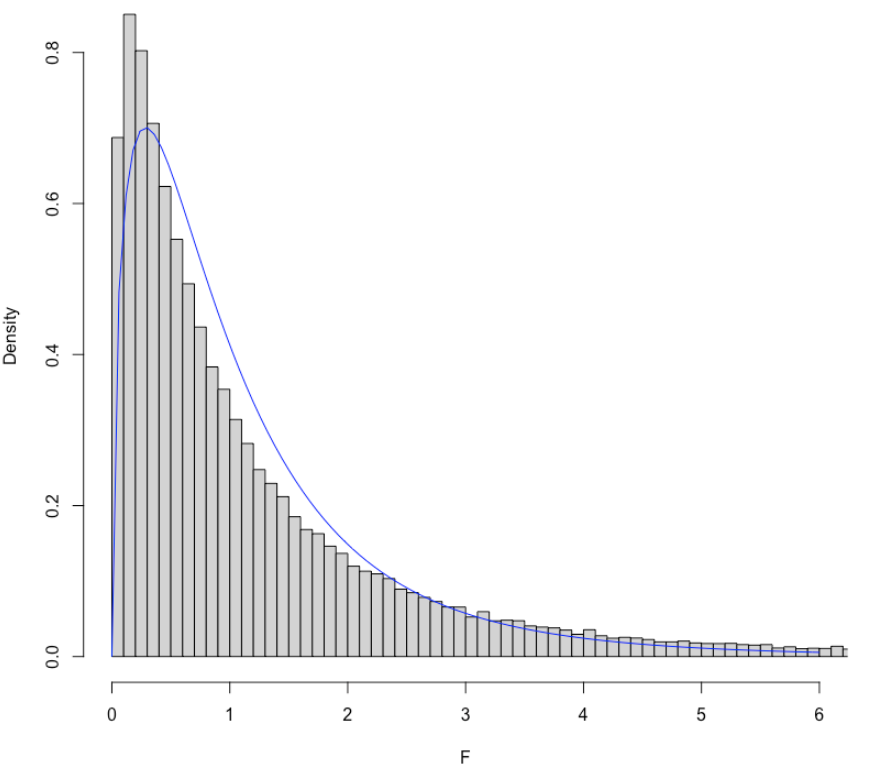
\includegraphics[width=0.85\linewidth]{_images/SamplingDistribF_false} 

}

\caption{Sampling distribution empirica per F, in caso di disomogeneità delle varianze. Vediamo che, in questo caso, la funzione di densità F di Fisher non costituisce un buon riferimento per il calcolo del P-level.}\label{fig:figName101a}
\end{figure}

\end{document}
